%input macros (i.e. write your own macros file called MacroFile1.tex)
%\include{Macros/MacroFile1}
\documentclass[oneside,12pt]{IIScthesisPSnPDF}



% \pagestyle{bfheadings}
%\usepackage{psfig}
% \usepackage{graphicx}
\usepackage{latexsym}
\usepackage{multicol}
\usepackage{booktabs}
\usepackage{multirow}
\usepackage{rotating}
\usepackage{hyperref}
\usepackage{fancyhdr}
\usepackage[numbers]{natbib}
\usepackage{wrapfig}
%\usepackage{algorithm}
%\usepackage{algorithmic}
\usepackage{enumerate}
%\usepackage{enumitem}
\usepackage{cancel}
\usepackage{mathrsfs}
% \usepackage{sfgame}
\usepackage{color}
\usepackage[compact]{titlesec}
\usepackage{mdwlist}
\usepackage{tikz}
\usepackage{varwidth}
\usepackage[vertfit]{breakurl}
\usepackage{datetime}
\usepackage{pdfpages}
\usepackage{dsfont}
% *** SUBFIGURE PACKAGES ***
\usepackage{subfig}
% \usepackage{biblatex}
\usetikzlibrary{shapes,arrows, trees}
\newtheorem{cons}{Constraint}

% ########### newly added
%\usepackage[showframe=true]{geometry}
\usepackage{changepage}
% wide page for side by side figures, tables, etc
\newlength{\offsetpage}
\setlength{\offsetpage}{2cm}

\newenvironment{widepage}{\begin{adjustwidth}{-\offsetpage}{-\offsetpage}%
    \addtolength{\textwidth}{2\offsetpage}}%
{\end{adjustwidth}}
%\usepackage[T1]{fontenc}

%\usepackage{polski}
%\usepackage[utf8]{inputenc}
%\usepackage[french,polutonikogreek,polish]{babel}

% *** MATH PACKAGES ***
\usepackage{amsmath}
\usepackage{amssymb}
\usepackage{amsthm}
\usepackage{mathtools}
\DeclarePairedDelimiter{\ceil}{\lceil}{\rceil}
%\DeclarePairedDelimiter\abs{\lvert}{\rvert}%
\DeclarePairedDelimiter\norm{\lVert}{\rVert}%

\usepackage{cleveref}

\usepackage{textcomp}
\usepackage{xspace}
\usepackage{listings}
\lstset{
  basicstyle=\ttfamily,
  mathescape
}
\usepackage{algorithmicx}
\usepackage{algpseudocode}
\usepackage[ruled]{algorithm}
\usepackage{theoremref}
\definecolor{light-gray}{gray}{0.75}
\algrenewcommand{\algorithmiccomment}[1]{\hskip3em{{\footnotesize \textcolor{light-gray}{$\blacktriangleright$}}} #1}
% define repetitive complex fragments here
\newcommand{\floe}{$\mathcal{F}{\ell}{o}{\varepsilon}$\xspace}
\newcommand{\dij}{\emph{Dijkstra's}\xspace}
\newcommand{\prc}{\mathcal{P}}
\newcommand{\chn}{\mathcal{C}}

\newcommand{\ystrim}[1]{}
\newtheorem{prop}{Proposition}
\newtheorem{conj}{Conjecture} 
\newtheorem{theorem}{Theorem}
\newtheorem{defn}{Definition}
\newtheorem{lemma}{Lemma}
\newtheorem{remark}{Remark}
\newtheorem{assumption}{Assumption}
\newcommand\floor[1]{\lfloor#1\rfloor}
%\newcommand\ceil[1]{\lceil#1\rceil}


%\usepackage[svgnames, x11names]{xcolor}
\newcommand{\ysnote}[1]{ {\textcolor{magenta} { ***Yogesh: #1 }}}

%\newcommand{\ysnoted}[1]{ {\textcolor{green} { ***TODO Later: #1 }}} %% COMMENT FOR FINAL THESIS VERSION
\newcommand{\ysnoted}[1]{} %% UNCOMMENT FOR FINAL THESIS VERSION

\newcommand{\scnote}[1]{ {\textcolor{orange} { ***Shayal: #1 }}}

\newcommand{\Note}[1]{ {\textcolor{red} {#1}}}

\newcommand{\csurnote}[1]{}

% Change tracking for article revisions. Added, Deleted, Replaced, or Modified content.
%
\usepackage[normalem]{ulem} % required for strikeout font


\newcommand{\modc}[1]{{\textcolor{blue}{#1}}}
\newcommand{\addc}[1]{{\textcolor{teal}{#1}}}
\newcommand{\delc}[1]{ {\textcolor{gray} {\sout{#1}} }}
%\newcommand{\delc}[1]{} % uncomment this (and comment above line) to ignore showing deletion
\newcommand{\repc}[2]{ {\textcolor{gray} {\sout{#1}} }{\textcolor{teal} {#2}}}
%\newcommand{\repc}[2]{{\textcolor{teal}{#2}}} % uncomment this (and comment above line) to ignore showing deletion
%\newcommand{\addc}[1]{#1}
%
%---------------------------------------------------------

%\input{preamble}

% \newcommand{\nobibentry}[1]{{\let\nocite\ignore\bibentry{#1}}}
\newdateformat{monthyeardate}{ \monthname[\THEMONTH], \THEYEAR}
\newcommand{\sn}[1]  {\noindent \textcolor{blue}{{\bf SN: }{``{\em #1}''}}}
\newcommand{\blankpage}{
\newpage
\thispagestyle{empty}
\mbox{}
\newpage
}

\newcommand{\blankpagewithnumber}{
\newpage
% \thispagestyle{empty}
\mbox{}
\newpage
}

\crefname{observation}{observation}{observations}
\crefname{algorithm}{algorithm}{algorithms}
\crefname{align}{equation}{equations}
\crefname{eqnarray}{equation}{equations}

% turn of those nasty overfull and underfull hboxes
\hbadness=10000
\hfuzz=50pt

% Put all the style files you want in the directory StyleFiles and usepackage like this:
% \usepackage{StyleFiles/watermark}

% Comment out the next line to get single spacing
\onehalfspacing
\allowdisplaybreaks
%\usepackage{fontspec}
%\newfontfamily\kannadafont{Noto Sans Kannada}
%\usepackage{polyglossia}
%\setmainlanguage{kannada}

\begin{document}

\title{Sequential Controlled Sensing to Detect \\ an Anomalous Process
} 

\submitdate{\monthyeardate\today} 
%\me
\phd
%\mscengg
%\degree{Master of Science (Engineering)} 
\dept{Electrical Communication Engineering}
\faculty{Faculty of Engineering}
\author{Karthik Periyapattana Narayanaprasad}

% Using the watermark package which is in StyleFiles/
% and to remove DRAFT COPY ONLY appearing on the top of all pages comment out below line
%\watermark{DRAFT COPY ONLY}


\maketitle


%\begin{center}
%\LARGE{\underline{\textbf{Declaration of Originality}}}
%\end{center}
%\noindent I, \textbf{Karthik Periyapattana Narayanaprasad}, with SR No. \textbf{04-02-00-10-12-15-1-12538}, hereby declare that
%the material presented in the thesis titled
%
%\begin{center}
%\textbf{Sequential Controlled Sensing to Detect an Anomalous Process
%}
%\end{center}
%
%\noindent represents original work carried out by me in the \textbf{Department of Electrical Communication Engineering} at \textbf{Indian Institute of
%Science} during the years \textbf{2015-2021}.
%
%\noindent With my signature, I certify that:
%\begin{itemize}
%	\item I have not manipulated any of the data or results.
%	\item I have not committed any plagiarism of intellectual
%	property.
%	I have clearly indicated and referenced the contributions of
%	others.
%	\item I have explicitly acknowledged all collaborative research
%	and discussions.
%	\item I have understood that any false claim will result in severe
%	disciplinary action.
%	\item I have understood that the work may be screened for any form
%	of academic misconduct.
%\end{itemize}
%
%\vspace{20mm}
%
%\noindent {\footnotesize{Date: \today	\hfill	Student Signature}} \qquad
%
%\vspace{20mm}
%
%\noindent In my capacity as supervisor of the above-mentioned work, I certify
%that the above statements are true to the best of my knowledge, and 
%I have carried out due diligence to ensure the originality of the
%report.
%
%\vspace{20mm}
%
%\noindent  {\footnotesize{Advisor Name: Rajesh Sundaresan \hfill Advisor Signature}}
%
%
\blankpage

\vspace*{\fill}
\begin{center}
\large\bf \textcopyright \ Karthik Periyapattana Narayanaprasad\\
\large\bf \monthyeardate\today\\
\large\bf All rights reserved
\end{center}
\vspace*{\fill}
\thispagestyle{empty}

\blankpage

\vspace*{\fill}
\begin{center}
\large \it To my parents.
%\large Dedicated to \\[2em]
%\large \it The Lotus Feet of Gurudev\\[2em]
\end{center}

\vspace*{\fill}
\thispagestyle{empty}

\blankpage
%\includepdf[pages={1}]{declaration.pdf}

%\vspace*{\fill}
%\begin{tabular}{p{0.4\columnwidth}p{0.5\columnwidth}}
% {\em Signature of the Author}: & \dotfill \\
% & Your Name \\
% & Dept.\ of Computer Science and Automation \\ 
% & Indian Institute of Science, Bangalore \vspace{1in}\\
% {\em Signature of the Thesis Supervisor}: & \dotfill \\
% & Your Advisor's Name \\
% & Professor \\
% & Dept.\ of Computer Science and Automation \\ 
% & Indian Institute of Science, Bangalore
%\end{tabular}
%\vspace*{\fill}
%\thispagestyle{empty}

%\blankpage

%set the number of sectioning levels that get number and appear in the contents
\setcounter{secnumdepth}{5}
\setcounter{tocdepth}{3}

\frontmatter % book mode only
\pagenumbering{roman}


% \include{Dedication/dedication}


\prefacesection{Acknowledgements}
If there are two people to whom the beginning of this journey of PhD can be traced back to, they are Prof. Chandra R. Murthy of the Department of ECE, IISc, and Dr. K. G. Nagananda, a close colleague and a doting mentor of mine. While Prof. Chandra introduced me to the world of academic research and sowed in me the seeds that would later germinate and embrace the vast ocean that research is, Nanda taught me the art of searching for pearls hidden deep beneath this ocean. While one taught me how to fly long distances looking for a flower, the other taught me the art of sucking the ambrosia from the flower without robbing the flower of its form and fragrance. If not for these noble souls, I would not have had the courage to pursue PhD. I am immensely thankful to both of them.

In my search for pearls in the ocean of research, I found one in my adviser, Prof. Rajesh Sundaresan. From heartily welcoming me into his lab space to making me feel at home, from patiently making me understand my paltry background in mathematics to guiding me gracefully towards speaking fluently in a language that he naturally spoke, from giving me the space and time to do things at my own pace to encouraging me to do things in my own way, from being an astute adviser who recognises the many infirmities of his students to thinking many steps ahead towards turning them into strengths, Prof. Rajesh has been with me through the thick and thin of my PhD journey. In his absence, he has reminded me that he is the sturdy earth beneath my feet along this journey, always present and ever ready to take on weight. For all the important lessons in research and in life that Prof. Rajesh has taught me, I shall remain forever indebted to him. I hope to brighten the lives of many students in much the same way that Prof. Rajesh did of mine, perhaps the least I can do to carry forward his legacy.

I am thankful to Prof. Utpal Mukherji, Prof. Navin Kashyap, Prof. Himanshu Tyagi, and Prof. Parimal Parag for serving as lighthouses along the journey. Their words of encouragement during every step of my PhD have been invaluable. From providing me with multiple opportunities to work alongside them in various capacities, be as a teaching assistant or otherwise, to readily agreeing to serve as my professional referees, they have been a true source of support. In particular, I would like to thank Prof. Navin and Prof. Himanshu for serving on the annual progress review committee and providing a platform for me to share with them the difficulties I faced along the journey without the fear of being judged. 

I am immensely thankful to all the professors of the Department of ECE and the Department of Mathematics at IISc for the superior quality lectures that I was fortunate to listen to. I am also thankful to the professors and students of TIFR Mumbai, IIT Bombay, IIT Madras, ISI Bangalore, ISI Delhi, and ISI Kolkata for the opportunities given to me to attend many of their seminars, workshops and lectures, and present my work at these places on several occasions.

An integral part of my PhD journey, one that will stay the closest to my heart, is the people with whom I associated myself while at IISc. Kishan, Chatan, Nihesh, Sarath, Krishna, Prakash, Hemanth, Akhil, Thiru, Nidhin, Bharath, Surabhi, Vinay, Garima, Chinmaya, Hari, Lakshmi Priya, Prathamesh, Sahasranand, Lekshmi, Bala, Sarvendranath, Vaishali, Rooji, Tarun -- these names will stay etched in my heart for the rest of my life. There are many more names that I have not mentioned here, courtesy paucity of space. 

This work was supported in part by the Science and Engineering Research Board (SERB) of the Department of Science and Technology, in part by the Ministry of Human Resource Development, Government of India, in part by the Centre for Networked Intelligence (CNI), IISc, and in part by the Robert Bosch Center for Cyber-Physical Systems (RBCCPS), IISc. I am thankful to RBCCPS for providing me the monetary support to travel to France to present my work at the 2019 IEEE International Symposium on Information Theory (ISIT). I would like to thank Lalitha Bai and Mr. Srinivasamurthy for extending support to me in matters concerning travel and disbursement of salary on a regular basis. 

This journey could not have been completed without the blessings of my parents and my gurus. I am thankful to Providence for gifting me a loving sister who cared for our parents in my absence. I am indebted to the many relatives whose love, care and words of encouragement kept me going along the journey. I only regret not being able to give them a satisfactory reply every time they asked me how much longer it would take me to finish my PhD studies. I am glad that they will not have to ask me anymore! 











\prefacesection{Abstract}
%Imagine a visual search experiment in which a number of static images are shown at once, with one oddball image in a sea of distracter images. The goal is to find the location of the oddball image as quickly as possible, subject to an upper bound on the probability of error. Vaidhiyan et al. \cite{vaidhiyan2018learning, vaidhiyan2017learning} modeled the above visual search experiment as a problem of finding an anomalous arm in a multi-armed bandit. Similar experiments, but with static images replaced by dynamic drifting-dots images (movies), were conducted by neuroscientists to see how evidence is accumulated in slow perceptual decision making. In these experiments, the dots executed Brownian motions with a fixed drift at each location. Moreover, the drifts were identical in distracter locations and were different from the drift in the oddball location. A systematic analysis of this visual search, along the lines of that carried out by Vaidhiyan et al., requires an understanding of the so-called restless odd Markov arm problem that forms the main subject of this thesis.
%
%Formally, we 


%Consider a multi-armed bandit with $K\geq 3$ arms in which each arm is a time homogeneous and ergodic discrete time Markov process evolving on a common finite state space. Suppose that one of the arms is anomalous in that its transition probability matrix (TPM) is $P_1$ and that of each non-odd arm is $P_2\neq P_1$. The TPMs $P_1$ and $P_2$ may or may not be known to a learning agent whose goal it is to find the anomalous arm (or odd arm) as quickly as possible, subject to an upper bound on error probability. The learning agent samples the arms sequentially, one at a time, until it is sufficiently confident of its knowledge of the odd arm. While the learning agent observes only one arm at any given time, the unobserved arms may either remain frozen until their next sampling time instant (rested arms) or continue to evolve (restless arms). Prior works have analysed the above problem for the case when each arm yields independent and identically distributed observations. We provide the first known extensions to the case of Markov observations from each arm.
%
%In the first part of this thesis, we analyse the setting of rested arms as a first step towards analysing the more difficult setting of restless arms. Here, we assume that the TPMs $P_1$ and $P_2$ are not known beforehand. We present an asymptotic lower bound on the expected time to find the odd arm, where the asymptotics is as the error probability vanishes. Further, we devise a sequential arm selection policy based on the principle of certainty equivalence and demonstrate that our policy achieves an upper bound that matches with the lower bound asymptotically. A key component in our analysis of the lower and the upper bounds is the identification of the fact that for the Markov process of each arm, the long term fraction of entries into a state is equal to the long term fraction of exits from the state (global balance). Both these quantities are in turn equal to the probability of observing the state under the arm's stationary distribution. 
%
%In the second part of this thesis, we derive the results for the setting of restless arms assuming that the TPMs $P_1$ and $P_2$ are known beforehand. The restless nature of the arms makes it necessary for the learning agent to keep track of the time since each arm was last sampled (arm's delay) and the state of each arm when it was last sampled (arm's last observed state). We introduce the notion of trembling hand. Under this trembling hand model, we derive an asymptotic lower bound on the expected time to find the odd arm, devise a sequential arm selection policy, and show that our policy achieves an upper bound that matches with the lower bound asymptotically as the error probability vanishes. In our analysis, we show that the arm delays and the last observed states form a controlled Markov process (a Markov decision problem (MDP)) which is ergodic under any stationary arm selection policy. Our approach of considering the delays and the last observed states of all the arms jointly offers a global perspective of the arms and serves as a `lift' from the local perspective of dealing with the delay and the last observed state of each arm separately (as suggested by the prior works). 
%In the absence of the trembling hand, we argue that it is not clear if the resulting lower and the upper bounds on the expected time to find the odd arm match.

%In the third and final part of this thesis, we extend the results of the previous part to the case when the TPMs $P_1$ and $P_2$ are not known beforehand and must be learnt along the way. Here too, we provide an asymptotic lower bound on the expected time required to find the odd arm. Because the TPMs are not known beforehand, we estimate the TPMs using maximum likelihood (ML) estimation. The key challenge here is in showing that the ML estimates of the TPMs converge to their true values, i.e., the system is identifiable. We prove identifiability under a continuous selection assumption and a certain regularity assumption on the TPMs. We devise a sequential arm selection policy based on the principle of certainty equivalence and show that it achieves an upper bound that matches with the lower bound asymptotically. Our achievability analysis relies crucially on resolving the identifiability problem. 
%We argue that for simpler policies that estimate the TPMs by repeated sampling of each arm before switching to another arm, it is not clear if the lower bound can be achieved or if the desired error probability can be met.

 
In this thesis, we study the problem of identifying an anomalous arm in a multi-armed bandit as quickly as possible, subject to an upper bound on the error probability. Also known as odd arm identification, this problem falls within the class of optimal stopping problems in decision theory and can be embedded within the framework of active sequential hypothesis testing. Prior works on odd arm identification dealt with independent and identically distributed observations from each arm. We provide the first known extension to the case of Markov observations from each arm. Our analysis and results are in the asymptotic regime of vanishing error probability.

We associate with each arm an ergodic discrete time Markov process that evolves on a common, finite state space. The notion of anomaly is that the transition probability matrix (TPM) of the Markov process of one of the arms (the {\em odd arm}) is some $P_{1}$, and that of each non-odd arm is a different $P_{2}$, $P_{2}\neq P_{1}$. A learning agent whose goal it is to find the odd arm samples the arms sequentially, one at any given time, and observes the state of the Markov process of the sampled arm. The Markov processes of the unobserved arms may either remain frozen at their last observed states until their next sampling instant ({\em rested arms}) or continue to undergo state evolution ({\em restless arms}). The TPMs $P_{1}$ and $P_{2}$ may be known to the learning agent beforehand or unknown. We analyse the following cases: (a) rested arms with TPMs unknown, (b) restless arms with TPMs known, and (c) restless arms with TPMs unknown. For each of these cases, we first present an asymptotic lower bound on the {\color{black} growth rate of the }expected time required to find the odd arm, and subsequently devise a sequential arm selection policy which we show achieves the lower bound and is therefore asymptotically optimal. 

A key ingredient in our analysis of the setting of rested arms is the observation that for the Markov process of each arm, the long term fraction of entries into a state is equal to the long term fraction of exits from the state (global balance). When the arms are restless, it is necessary for the learning agent to keep track of the time since each arm was last sampled (arm's {\em delay}) and the state of each arm when it was last sampled (arm's {\em last observed state}). We show that the arm delays and the last observed states form a controlled Markov process which is ergodic under any stationary arm selection policy that picks each arm with a strictly positive probability. Our approach of considering the delays and the last observed states of all the arms jointly offers a global perspective of the arms and serves as a `lift' from the local perspective of dealing with the delay and the last observed state of each arm separately, one that is suggested by the prior works. Lastly, when the TPMs are unknown and have to be estimated along the way, it is important to ensure that the estimates converge almost surely to their true values asymptotically, i.e., the system is {\em identifiable}. We show identifiability follows from the ergodic theorem in the rested case, and provide sufficient conditions for it in the restless case.













\blankpage
\tableofcontents
\blankpage
\listoffigures
%\ysnote{Verify that the figure captions are meaningful and self-contained when appearing in the TOC.}


%\listoftables
%\ysnote{table captions must be more descriptive. it is ambiguous when it appears on the TOC.}
\blankpage
\prefacesection{Publications Based on this Thesis}
\begin{enumerate}[1.]
\item P. N. Karthik, R. Sundaresan, {\em Learning to Detect an Odd Restless Markov Arm with a Trembling Hand}, submitted.
\item P. N. Karthik, R. Sundaresan, {\em Detecting an Odd Restless Markov Arm with a Trembling Hand}, IEEE Transactions on Information Theory, July 2021.
\item P. N. Karthik, R. Sundaresan, {\em Learning to Detect an Odd Markov Arm}, IEEE Transactions on Information Theory, July 2020, vol. 66, no. 7, pp. 4324 – 4348.
\item P. N. Karthik, R. Sundaresan, {\em Learning to Detect an Odd Restless Markov Arm},  
proceedings of the 2021 IEEE International Symposium on Information Theory (ISIT), virtual conference.
\item P. N. Karthik, R. Sundaresan, {\em Detecting an Odd Restless Markov Arm with a Trembling Hand}, proceedings of the 2020 IEEE International Symposium on Information Theory (ISIT), virtual conference.
\item P. N. Karthik, R. Sundaresan, {\em Learning to Detect an Odd Markov Arm}, proceedings of the 2019 IEEE International Symposium on Information Theory (ISIT), Paris, France, July 2019. 
\end{enumerate}

%\blankpagewithnumber
% \printnomenclature  %% Print the nomenclature
% \addcontentsline{toc}{chapter}{Nomenclature}

\mainmatter % book mode only
\setcounter{page}{1}

\chapter{Introduction}
\label{ch:introduction}

%Imagine a visual search experiment in which a number of static images are shown at once, with one oddball image in a sea of distracter images. The goal is to find the location of the oddball image as quickly as possible, subject to an upper bound on the probability of error. Vaidhiyan et al. \cite{vaidhiyan2017learning, vaidhiyan2017learning} modeled the above visual search experiment as a problem of finding an anomalous arm in a multi-armed bandit. Similar experiments, but with static images replaced by dynamic drifting-dots images (movies), were conducted by neuroscientists \cite{krueger2017evidence} to see how evidence is accumulated in slow perceptual decision making. In these experiments, the dots executed Brownian motions with a fixed drift at each location. Moreover, the drifts were identical in distracter locations and were different from the drift in the oddball location. A systematic analysis of this visual search, along the lines of that carried out by Vaidhiyan et al., requires an understanding of the so-called restless odd Markov arm problem that forms the main subject of this thesis.
%
%For the purposes of carrying out mathematical analysis, the visual search experiments described above may be cast as a problem of identifying an anomalous Markov process in a multi-armed bandit in the following way.  

Suppose that a decision entity wishes to select a subset of one or more alternatives among a fixed number of alternatives, each of which yields a random reward from an unknown distribution upon being selected. In the face of uncertainty, the decision entity must select the alternatives sequentially in a way so as to maximise its overall reward accumulated over a finite time horizon of $T$ time instants or an infinite time horizon. Such examples of decision making under uncertainty are popularly modeled using {\em multi-armed bandits} in which an arm is analogous to an altenative. Defining {\em regret} of an arms selection strategy (policy) as the difference between the total expected reward obtained under the policy and the total reward obtained under a policy which knows the reward distributions, the goal of the decision entity is, equivalently, to repeatedly sample the arms so as to minimise the finite or the infinite time horizon regret. Typically, the successive rewards from any given arm are assumed either to be independent and identically distributed (iid) or to have a first order dependence (Markov), and independent of the rewards of the other arms.


%Multi-armed bandits constitute a popular model for decision making under uncertainty. The classical setup of multi-armed bandits consists of a fixed number of alternatives (called {\em arms}) competing for a common resource that can sample a subset of arms at any given time. Each arm, upon being sampled, yields a random reward whose distribution is unknown to a decision entity. The goal of the decision entity is to sample the arms in such a way that the expected sum of rewards accumulated over a finite horizon of $T$ time instants  is maximised. 

While one line of works on multi-armed bandits is based on the theme of maximising rewards (or equivalently minimising regret) as described above, another line of works focuses on the theme of {\em optimal stopping} where the goal is to test for the validity of one or more hypotheses as quickly as possible and stop further sampling of the arms. For instance, the problem of best arm identification \cite{kaufmann2016complexity} in which the goal is to find the index of the arm that yields the largest mean reward as quickly as possible and stop, is an example of an optimal stopping problem in multi-armed bandits. Another instance of an optimal stopping problem in multi-armed bandits, one that constitutes the main topic of this thesis, is the problem of {\em odd arm identification} in which one of the arms in the multi-armed bandit is anomalous, and the goal is to find the index of the anomalous arm (or {\em odd arm}) as quickly as possible. It is interesting to note here that the arm sampling policies that are optimal in the context of reward maximisation (or regret minimisation) may not necessarily be so for optimal stopping problems; we refer the reader to \cite{Bubeck2011} for a discussion on this. 
%Additionally, when studying optimal stopping problems in multi-armed bandits, the notion of rewards may be discarded as the goal is not to maximise rewards. Instead, the state of a sampled arm may be treated as merely an observation from the arm. 

In this thesis, we study of the problem of odd arm identification in the setting when the successive observations from each arm form a Markov process. In this context, anomaly simply means that the transition probability matrix (TPM) of the odd arm is $P_1$, and that of each non-odd arm is $P_2$, where $P_2\neq P_1$. Throughout the thesis, we study the close interplay between the following important quantities that dictate the performance of any arm sampling policy: (a) the time to stoppage, i.e., the time to identify the index of the odd arm, and (b) the error probability at stoppage. For the purpose of carrying out analysis, it is customary to fix one of these quantities and study the behaviour of the other in terms of the quantity fixed. In this thesis, we fix the error probability and characterise the asymptotic behaviour of the time to stoppage as a function of the error probability, where the asymptotics is as the error probability vanishes. 

\section{Motivation}
Our motivation to study the problem of odd arm identification in the setting of Markov observations from the arms comes from the desire to extend, to more general settings, the decision theoretic formulation of a certain visual search experiment conducted by Sripati and Olson \cite{sripati2010global} and analysed in Vaidhiyan et al. \cite{Vaidhiyan2017,vaidhiyan2012active}. In this experiment, human subjects were shown a number of images at once, with one {\em oddball} image in a sea of {\em distracter} images. The goal of the experiment was to understand the relationship between (a) the average time taken by the human subject to identify the oddball image, and (b) the dissimilarity between the oddball and distracter images as perceived by the human subject. Vaidhiyan et al. modelled visual search for locating an oddball image in a sea of distracter images, as quickly as possible, as an odd arm identification problem with Poisson observations. The Poisson observations stemmed from the Poisson point process model for the neuron firings when the human subject focuses on a particular image, the analogue of pulling an arm. They showed that dissimilarity in neural responses to the oddball and the distracter images predicted the time taken by human subjects in detecting the location of the oddball image. The analysis was extended to the case when the parameters of the process were unknown, but had to be learnt during search, in \cite{vaidhiyan2017learning}. 


The oddball and distracter images in the experiments analysed in Vaidhiyan et al. \cite{Vaidhiyan2017, vaidhiyan2012active, vaidhiyan2017learning} and in Sripati and Olson \cite{sripati2010global} were static images. Similar experiments, but with dynamic drifting-dots images (movies), as in Krueger et al. \cite{krueger2017evidence}, were conducted by Vaidhiyan et al. to see how evidence is accumulated in slow perceptual decision making. In these experiments, the dots executed Brownian motions with a fixed drift at each location. Moreover, the drifts were identical in the distracter locations and were different from the drift in the oddball location. Subjects had to identify the oddball (anomalous) movie location as quickly as possible. A proper analysis of this visual search, along the lines of  \cite{Vaidhiyan2017}, \cite{vaidhiyan2012active} and \cite{vaidhiyan2017learning}, requires an understanding of the so-called \emph{restless} odd Markov arm problem where\footnote{The correspondence between the oddball movie experiment and the restless odd Markov arm problem is as follows: an arm corresponds to a movie; an observation from an arm corresponds to the positions of the dots in a movie frame; the Markov relationship between the successive observations from an arm corresponds to the dependence between the positions of the dots in the successive frames of a movie.} each arm yields Markov observations, one of the arms is anomalous, and the states of the unobserved arms continue to change (restless arms). Indeed, in the aforementioned drifting-dots experiment, the positions of the dots (state) will have changed when the subject returns to observe a particular location after a decision to look at another location. An analysis of the restless odd Markov arm problem forms the main subject of this thesis.

 
\section{Prior works on Odd Arm Identification}
The problem of odd arm identification has been studied in the literature for the case of independent and identically distributed (iid) observations from each arm. The works of Vaidhiyan et al. \cite{Vaidhiyan2017, vaidhiyan2012active, vaidhiyan2017learning} study the case of iid, indeed Poisson, observations from each arm. Prabhu et al. \cite{prabhu2017learning} extend the analysis of Vaidhiyan et al. to the case of iid observations belonging to a generic exponential family. The works  \cite{Vaidhiyan2017}, \cite{vaidhiyan2012active}, \cite{vaidhiyan2017learning} and \cite{prabhu2017learning}  can be embedded within the classical works of Chernoff \cite{Chernoff1959} and Albert \cite{albert1961sequential},  and provide a general framework for the analysis of lower bounds on expected number of samples required for identifying the index of the odd arm. In addition, they also provide explicit policies  that achieve these lower bounds in the asymptotic regime as error probability vanishes. We refer the reader to also \cite{kaufmann2016complexity,garivier2016optimal,hemo2016asymptotically,nitinawarat2017,naghshvar2010active,naghshvar2010information,naghshvar2011performance,naghshvar2013active} for other related works on iid observations. While the aforementioned works deal with iid arms, the novelty in this paper is that we consider Markov arms. To the best of our knowledge, we believe that our work is the first to consider Markov arms in the context of odd arm identification.

\section{Problem Setup and Objective}
Formally, our problem setup is as follows. We consider a multi-armed bandit with $K\geq 3$\footnote{This ensures that the notion of an ``odd'' arm makes sense.} arms. We associate with each arm a time homogeneous and ergodic discrete time Markov process evolving on a common, finite state space. We assume that the TPM of the odd arm is $P_{1}$ and that of each non-odd arm is $P_{2}\neq P_{1}$. Given an error probability threshold $\epsilon>0$, a learning agent wishes to identify the index of the odd arm as quickly as possible, subject to its error probability not exceeding $\epsilon$. The learning agent may or may not possess the knowledge of the TPMs of the arms, and samples the arms sequentially, one at any given time, until it is sufficiently confident of which arm is the odd arm. While the learning agent observes only one arm at any given time, the unobserved arms continue to evolve (restless arms). 

Suppose $\pi$ is an arm selection {\em policy} of the learning agent whose time to find the odd arm is $\tau(\pi)$. Given $\epsilon>0$, let $\Pi(\epsilon)$ denote the collection of all policies whose error probability is at most $\epsilon$. Let $C=(h, P_{1}, P_{2})$ denote an arms configuration in which $h$ is the index of the odd arm, $P_{1}$ is the TPM of arm $h$ and $P_{2}$ is the TPM of each non-odd arm $a\neq h$. Writing $E^{\pi}[\cdot|C]$ to denote the expectation computed under the policy $\pi$ and under the arms configuration $C$, an examination of the prior works reveals that $$ \inf\limits_{\pi\in \Pi(\epsilon)} E^{\pi}[\tau(\pi)|C] = O\left(\log \frac{1}{\epsilon}\right); $$ the constant multiplying $\log (1/\epsilon)$ in the above equation is, in general, a function of the arms configuration $C$. Our objective is to characterise
\begin{align}
\lim\limits_{\epsilon\downarrow 0}  \inf\limits_{\pi\in \Pi(\epsilon)} \frac{E^{\pi}[\tau(\pi)|C]}{\log (1/\epsilon)}.
\label{eq:intro_main_problem}
\end{align}
That is, our interest is to capture mathematically the asymptotic growth rate of the expected time required to find the odd arm subject to an upper bound on the error probability, where the asymptotics is as the error probability vanishes.

\section{Our Contributions}
Although our end goal is to study the restless odd Markov arm problem, the continued evolution of the arms in the restless setting presents many challenges in the analysis. Therefore, as a key first step towards an understanding of the restless setting, we analyse the simpler setting of {\em rested} arms in which the unobserved arms do not evolve and remain frozen at their previously observed states. For the settings of rested arms and restless arms, we provide answers to \eqref{eq:intro_main_problem} by first deriving a problem-instance dependent (arms configuration dependent) lower bound for \eqref{eq:intro_main_problem}. We show that the lower bound is of the form $1/\alpha(h, P_{1}, P_{2})$, where the constant $\alpha(h, P_{1}, P_{2})$ captures the hardness of the problem: the closer the TPMs $P_{1}$ and $P_{2}$ are (in an appropriately defined sense), the smaller the value of $\alpha$ is, and therefore the larger the lower bound, thereby implying longer times to find the odd arm. The exact form of $\alpha(h, P_{1}, P_{2})$ depends on whether or not the TPMs $P_{1}$ and $P_{2}$ are known to the learning agent beforehand. Complementing the lower bound results in each of the above cases (rested/restless, TPMs unknown/known), we devise a sequential arm selection policy and demonstrate that the expected time for the policy to find the odd arm satisfies an asymptotic upper bound that is equal to $1/\alpha(h, P_{1}, P_{2})$. Thus, our answer to \eqref{eq:intro_main_problem} is $1/\alpha(h, P_{1}, P_{2})$, where $\alpha(h,P_1,P_2)$ depends on whether the arms are rested/restless, whether the TPMs $P_1$ and $P_2$ are known or unknown, etc. From the symmetry of the problem, it can be deduced that $\alpha(h,P_1,P_2)$ does not depend on $h$, the index of the odd arm. 

\section{Organisation of the Thesis}
This thesis is organised as follows. In Chapter \ref{ch:rested_arms}, we analyse the setting of rested arms when the TPMs $P_1$ and $P_2$ are not known beforehand\footnote{The case of known TPMs in the setting of rested arms is a straighforward extension of the case of iid observations from the arms, and is therefore omitted.}. A key component in our analysis of the lower and the upper bounds for this case is the identification of the fact that for the Markov process of each arm, the long term fraction of entries into a state is equal to the long term fraction of exits from the state (global balance). Both these quantities are in turn equal to the probability of observing the state under the arm's stationary distribution.

In Chapter \ref{ch:restless_with_known_TPMs}, we derive the results for the setting of restless arms assuming that the TPMs $P_1$ and $P_2$ are known beforehand. The restless nature of the arms makes it necessary for the learning agent to keep track of the time since each arm was last sampled (arm's delay) and the state of each arm when it was last sampled (arm's last observed state). We introduce the notion of ``trembling hand'' commonly observed in visual search experiments, in which at any given time the learning agent intends to sample a certain arm but the actual arm sampled differs from the intended arm with a small probability. We show that the arm delays and the last observed states form a controlled Markov process which, under the trembling hand model, is ergodic under any stationary arm selection policy. Our approach of considering the delays and the last observed states of all the arms jointly offers a global perspective of the arms and serves as a `lift' from the local perspective of dealing with the delay and the last observed state of each arm separately (as done in the prior works). In the absence of the trembling hand, we discuss the difficulties associated with showing that the lower and the upper bounds match.

In Chapter \ref{ch:restless_with_unknown_TPMs}, we extend the results of Chapter \ref{ch:restless_with_known_TPMs} to the case when the TPMs $P_1$ and $P_2$ are not known beforehand and must be learnt along the way. Here, we estimate the TPMs using maximum likelihood (ML) estimation. The key challenge here is in showing that the ML estimates of the TPMs converge to their true values, i.e., the system is {\em identifiable}. We prove identifiability under a continuous selection assumption and a certain regularity assumption on the TPMs. Our achievability (upper bound) analysis relies crucially on resolving the identifiability problem. For a simpler policy that estimates the TPMs by repeated sampling of each arm before switching to another arm, we highlight the difficulties  in achieving the lower bound and meeting the desired error probability.

We conclude the thesis in Chapter \ref{ch:conclusions_and_future_work} and propose some future directions for exploration.


%\vspace{0.5cm}
%\textbf{A simplified model and our contributions} 
% . Broadly, we study the problem of odd arm identification in the following settings: 
%\begin{itemize}
%	\item Arms are rested and the TPMs $P_1$ and $P_2$ are not known beforehand.
%	\item Arms are restless and the TPMs $P_1$ and $P_2$ are known beforehand.
%	\item Arms are restless and the TPMs  $P_1$ and $P_2$ are not known beforehand.
%\end{itemize}
%For each of the above settings, we first present an asymptotic lower bound on the expected time to find the location of the odd arm, where the asymptotics is as the error probability vanishes. Subsequently, we show that in each of the above settings, there exists a policy which achieves the lower bound asymptotically. We provide an explicit description of the policy for each setting. We omit the analysis of the case when the arms are rested and the TPMs $P_1$ and $P_2$  are known beforehand as this is subsumed by the case of unknown $P_1$ and $P_2$. Our results  generalise the results of the prior works  \cite{vaidhiyan2017learning, Vaidhiyan2017, prabhu2017learning} to the case of Markov observations.
%
%In our analysis of the setting of rested arms, we bring out the key idea that any two successive selections of an arm result in observing a transition from the state corresponding to the arm's first selection to the state corresponding to the arm's second selection. As a consequence, for each state in the state space, the empirical proportion of times an arm occupies the state prior to a transition is equal, in the long run, to the empirical proportion of times the arm occupies the state after a transition. We then replace these common proportions by the probability of the arm occupying this state under its stationary distribution. Such a replacement by stationary probabilities is possible mainly due to the rested nature of the arms, and may not be possible in more general settings such as when the arms are restless. Identifying invariant quantities, such as the long-term fraction of exits and entries from a state in this case, lies at the heart of our analysis. When the arms are restless, 
%
%
%
%
%
%
%
%
%

\blankpage
\chapter{Rested Arms}
\label{ch:rested_arms}
\section{Preamble}

In this chapter, we analyse the setting of rested arms with TPMs unknown. That is, given a multi-armed bandit with $K\geq 3$ arms and an arms configuration $C=(h, P_{1}, P_{2})$ in which $h$ is the index of the odd arm, the TPM of arm $h$ is $P_{1}$, and the TPM of each of the remaining arms is $P_{2}\neq P_{1}$, we wish to characterise $$ \lim\limits_{\epsilon\downarrow 0}  \inf\limits_{\pi\in \Pi(\epsilon)} \frac{E^{\pi}[\tau(\pi)|C]}{\log (1/\epsilon)} $$ for the setting of rested arms when $P_{1}$ and $P_{2}$ are not known beforehand. Our analysis of the setting of rested arms forms a key first step towards analysing the more difficult setting of restless arms. The rested case has its own interesting features. For example, as we shall see later in this chapter, the asymptotically optimal arm selection strategy does not explicitly depend on the last observed states of the arms. This, at first glance, is surprising.

\subsection{Prior Works on Rested Arms}
{One of the earliest works to consider the setting of rested arms is that of Gittins' \cite{gittins1979bandit} in which it is assumed that each arm yields a random `reward' when selected, and that the successive rewards from any given arm constitute a Markov process. In this reward setting, the central problem is one of maximising the infinite horizon average discounted reward. For this problem, Gittins proposed and demonstrated the optimality of a simple index-based policy that, at each time, involves constructing an index for every arm based on the knowledge of the transition laws of the arms and selecting an arm with the largest index. Agarwal et al. \cite{agrawal1989asymptotically} consider a similar setting as Gittins' in which each arm yields Markov rewards. However, unlike in  \cite{gittins1979bandit}, the authors of \cite{agrawal1989asymptotically} do not assume the knowledge of the transition laws of the arms. Instead, they assume that the transition law of each arm is parameterised by an unknown parameter belonging to a known, finite, parameter space. Define `regret' as the difference between the infinite time horizon expected sum of rewards generated by any policy and that generated by a policy which knows the parameters of the arms. The goal of the authors of \cite{agrawal1989asymptotically} is to design policies whose regret, in the asymptotic limit as time $n\to\infty$, is $o(n^\alpha)$ for every $\alpha>0$. For this problem, the authors of \cite{agrawal1989asymptotically} provide a lower bound in which the long-term regret grows asymptotically as $\log n$ times a multiplicative constant that captures the hardness of the problem. Furthermore, they propose a policy and demonstrate that it achieves the lower bound in the limit as $n\to \infty$.}

{While the aforementioned works deal with reward maximisation, and the associated regret minimisation in the unknown parameters setting, our problem is one of {\em optimal stopping}. We note that the lower bound in \cite{agrawal1989asymptotically}, although quantifying the asymptotic growth rate of regret, does not reflect the quickness of learning the underlying parameters of the arms. That is, the results in \cite{agrawal1989asymptotically} do not shed light on the minimum number of arm selections that are needed, on the average, in order to learn the parameters of the arms up to a desired level of accuracy. We answer this question when one of the arms is anomalous and the asymptotics is as the error probability vanishes. In doing so, we treat the state of any selected arm as merely a Markov observation from the arm and not as a reward, since our objective is one of optimal stopping and not of regret minimisation. We note here that policies which are optimal in the context of the problem studied here may not necessarily be optimal in the context of regret minimisation, and vice-versa; see Bubeck et al. \cite{Bubeck2011} for a discussion on this. Finally, the unknown parameters of our problem are the transition laws of the odd arm and the non-odd arm Markov processes, and the index of the odd arm, thus making our parameter set a continuum, unlike the finite parameter set considered in \cite{agrawal1989asymptotically}.}

Finally, a recent and independent work of Moulos \cite{moulos2019optimal} studies a closely related problem of \emph{best arm identification} in rested multi-armed bandits, where the goal is to find the arm with the largest stationary mean. The results presented in \cite{moulos2019optimal} are in terms of an asymptotic and a non-asymptotic lower bound, where the asymptotics is as the error probability vanishes, and a policy for best arm identification whose asymptotic upper bound is four times larger than the asymptotic lower bound. In this chapter, we present the first known asymptotic lower bound for the problem of odd arm identification, and an asymptotically optimal policy that meets the lower bound. This is in contrast with the gap between the upper bound and the lower bound in \cite{moulos2019optimal} for best arm identification. We anticipate that a policy similar to ours should close the gap between the upper and lower bounds in \cite{moulos2019optimal}.

\subsection{An Overview of Our Contributions}
Below, we highlight our contributions and bring out the challenges that we need to overcome in the analysis of the setting of rested arms.
\begin{enumerate}
    \item \textcolor{black}{In Section \ref{rested_arms_sec:lower_bound}}, we derive an asymptotic lower bound on {\color{black} the growth rate of} the expected number of arm selections required by any policy that the learning agent may use to identify the index of the odd arm. Here, the asymptotics is as the error probability vanishes. Similar to the lower bounds appearing in \cite{prabhu2017learning} and \cite{agrawal1989asymptotically}, our lower bound has a problem-instance (or arms configuration) dependent constant that quantifies the effort required by any policy to identify the true index of the odd arm by guarding itself against identifying the nearest, incorrect alternative. \textcolor{black}{This constant is a function of the transition probability matrices of the odd arm and the non-odd arms.}
    \item We characterise the growth rate of the expected number of arm selections required by any policy as a function of the maximum acceptable error probability, and show that in the regime of vanishingly small error probabilitys, this growth rate is logarithmic in the inverse of the error probability. The analysis of the lower bounds in \cite{vaidhiyan2017learning} and \cite{prabhu2017learning} uses the familiar data processing inequality presented in the work of Kaufmann et al. \cite{kaufmann2016complexity} that is based on Wald's identity \cite{wald1944cumulative} for iid processes. However, the Markov setting in our problem does not permit the use of Wald's identity. Therefore, we derive results for our Markov setting generalising those appearing in \cite{kaufmann2016complexity}, and subsequently use these generalisations to arrive at the lower bound. See Section \ref{rested_arms_sec:lower_bound} for the details.
    \item \textcolor{black}{In the analysis of the lower bound, we bring out the key idea that any two successive selections of an arm result in the learning agent observing a transition from the state corresponding to the arm's first selection to the state corresponding to the arm's second selection. As a consequence, for each state in the state space, the empirical proportion of times an arm occupies the state prior to a transition is equal, in the long run, to the empirical proportion of times the arm occupies the state after a transition. We then replace these common proportions by the probability of the arm occupying this state under its stationary distribution. Such a replacement by stationary probabilities is possible mainly due to the rested nature of the arms, and may not be possible in more general settings such as when the arms are restless.}
    \item \textcolor{black}{In Section \ref{rested_arms_sec:achievability}}, we propose a sequential arm selection scheme that takes as inputs two parameters, one of which may be chosen appropriately to meet the acceptable error probability, while the other may be tuned to ensure that the performance of our scheme comes arbitrarily close to the lower bound, thus making our scheme near-optimal.


    We now contrast the near-optimality of our scheme with the near-optimality of the scheme proposed by Vaidhiyan et al. in \cite{vaidhiyan2017learning}, and highlight a key simplification that our scheme entails. The scheme of Vaidhiyan et al. is built around the important fact that each arm is sampled at a non-trivial, strictly positive and optimal rate that is bounded away from zero, as given by the lower bound, thereby allowing for exploration of the arms in an optimal manner. This stemmed from their specific Poisson observations. However, the lower bound presented in Section \ref{rested_arms_sec:lower_bound} may not have this property
    %    does not allow for us to establish a similar fact
in the context of Markov observations.
    %see \cite[Assumption 4]{prabhu2017learning}. However, the authors of \cite{prabhu2017learning} establish the validity of their assumption only for some of the commonly used distributions belonging to the exponential family, thereby leaving open the validity of the assumption in full generality.
    Therefore, recognising the requirement of sampling the arms at a non-trivial rate for good performance of our scheme, in this chapter, we use the idea of ``forced exploration'' proposed by Albert in \cite{albert1961sequential}. In particular, we propose a simplified way of sampling the arms by considering a mixture of uniform sampling and the optimal sampling given by the lower bound in Section \ref{rested_arms_sec:lower_bound}. We do this by introducing an appropriately tuneable parameter that controls the probability of switching between uniform sampling and optimal sampling, the latter being given by the lower bound. While this ensures that our policy samples each arm with a strictly positive probability at each step, it also gives us the flexibility to select an appropriate value for this parameter so that the upper bound on the performance of our scheme may be made arbitrarily close to our lower bound. We refer the reader to Section \ref{rested_arms_sec:achievability} for the details.
\end{enumerate}

\subsection{Chapter Organisation}
The rest of this chapter is organised as follows. In Section \ref{rested_arms_sec:notations}, we set up the notations that will be used throughout the chapter. In Section \ref{rested_arms_sec:lower_bound}, we present a lower bound on the performance of any policy. In Section \ref{rested_arms_sec:achievability}, we present a sequential arm selection policy and demonstrate its near optimality. We present the main result of this chapter in Section \ref{rested_arms_sec:main_result}, combining the results of Sections \ref{rested_arms_sec:lower_bound} and \ref{rested_arms_sec:achievability}. In Section \ref{rested_arms_sec:simulation_results}, we provide some simulation to support the theoretical development. We present the proofs of all the results in Section \ref{rested_arms_sec:proofs_of_main_results}, and summarise the key points of this chapter in Section \ref{rested_arms_sec:conclusions}.

\section{Notations}
\label{rested_arms_sec:notations}
In this section, we set up the notations that will be used throughout the chapter. Let $K\geq 3$ denote the number of arms, and let $\mathcal{A}=\{1,2,\ldots,K\}$ denote the set of arms. We associate with each arm an irreducible, aperiodic, time homogeneous discrete-time Markov process on a finite state space $\mathcal{S}$, where the Markov process of each arm is independent of the Markov processes of the other arms. We denote by $|\mathcal{S}|$ the cardinality of $\mathcal{S}$. Without loss of generality, we take $\mathcal{S}=\{1,2,\ldots,|\mathcal{S}|\}$. Hereinafter, we use the phrase `Markov process of arm $a$' to refer to the Markov process associated with arm $a\in \mathcal{A}$.

At each discrete time instant, one out of the $K$ arms is selected and its state is observed. We let $A_n$ denote the arm selected at time $n$, and let $\bar{X}_n$ denote the state of arm $A_n$, where $n\in\{0,1,2,\ldots\}$. We treat $A_0$ as the zeroth arm selection and $\bar{X}_0$ as the zeroth observation. Selection of an arm at time $n$ is based on the history $(\bar{X}^{n-1},A^{n-1})$ of past observations and arms selected; here, $\bar{X}^k$ (resp. $A^k$) is a shorthand notation for the sequence $\bar{X}_0,\ldots,\bar{X}_k$ (resp. $A_0,\ldots,A_k$). We shall refer to such a sequence of arm selections and observations as a policy, which we generically denote by $\pi$. For each $a\in\mathcal{A}$, we denote the Markov process of arm $a$ by the collection $(X_k^a)_{k\geq 0}$ of random variables. Further, we denote by $N_a(n)$ the number of times arm $a$ is selected by a policy up to (and including) time $n$, i.e.,
\begin{equation}
N_a(n)=\sum\limits_{t=0}^{n}1_{\{A_t=a\}}.\label{rested_arms_eq:N_a(n)}	
\end{equation}
 Then, for each $n\geq 0$, we have the observation
\begin{equation}
	\bar{X}_n=X_{N_{A_n}(n)-1}^{A_n}.\label{rested_arms_eq:obs_at_time_n}
\end{equation}

We consider a scenario in which the Markov process of one of the arms (hereinafter referred to as the odd arm) follows a probability transition matrix $P_1=(P_1(j|i))_{i,j\in\mathcal{S}}$, while those of rest of the arms follow a probability transition matrix $P_2=(P_2(j|i))_{i,j\in\mathcal{S}}$, where $P_2\neq P_1$; here, $P(j|i)$ denotes the entry in the $i${th} row and $j$th column of the matrix $P$. Further, we let $\mu_1$ and $\mu_2$ denote the unique stationary distributions of $P_1$ and $P_2$ respectively. We denote by $\nu$ the common distribution for the initial state of each Markov process. In other words, for arm $a\in \mathcal{A}$, we have $X_0^a\sim \nu$, and this is the same distribution for all arms. We operate in a setting where the probability transition matrices and their associated stationary distributions are unknown to the learning agent.

For each $a\in\mathcal{A}$ and state $i\in \mathcal{S}$, we denote by $N_a(n,i)$ the number of times up to (and including) time $n$ the Markov process of arm $a$ is observed to \textcolor{black}{occupy state $i$ prior to a transition}, i.e.,
\begin{equation}
	N_a(n,i)=\sum\limits_{m=1}^{N_a(n)-1} 1_{\{X_{m-1}^a=i\}}.\label{rested_arms_eq:N_a(n,i)}
\end{equation}
Similarly, for each $i,j\in \mathcal{S}$, we denote by $N_a(n,i,j)$ the number of times up to (and including) time $n$ the Markov process of arm $a$ is observed to \textcolor{black}{make a transition from state $i$ to state $j$}, i.e.,
\begin{equation}
	N_a(n,i,j)=\sum\limits_{m=1}^{N_a(n)-1} 1_{\{X_{m-1}^a=i,\,X_m^a=j\}}.\label{rested_arms_eq:N_a(n,i,j)}
\end{equation}
Clearly, then, the following hold:
\begin{subequations}
\begin{enumerate}
	\item For each $a\in \mathcal{A}$ and $i\in\mathcal{S}$,
	\begin{equation}
		\sum\limits_{j\in\mathcal{S}}N_a(n,i,j)=N_a(n,i).\label{rested_arms_eq:sum_N_a(n,i,j)}
	\end{equation}
	\item For each $a \in \mathcal{A}$,
	\begin{equation}
		\sum\limits_{i\in\mathcal{S}}N_a(n,i)=N_a(n)-1.\label{rested_arms_eq:N_a_summed_over_i}
	\end{equation}
	\item For each $n$,
	\begin{equation}
		\sum\limits_{a\in\mathcal{A}}N_a(n)=n+1.\label{rested_arms_eq:sum_N_a}
	\end{equation}
\end{enumerate}
\end{subequations}
We note here that the upper index of the summation in \eqref{rested_arms_eq:N_a(n,i)} is $N_a(n)-1$, and not $N_a(n)$, since the last observed transition on arm $a$ would be from the state $X_{N_a(n)-2}^a$ to the state $X_{N_a(n)-1}^a$. This is further reflected by the summation in \eqref{rested_arms_eq:N_a_summed_over_i}.

Fix probability transition matrices $P_1$ and $P_2$, where $P_2\neq P_1$, and let $H_{h}$ denote the hypothesis that $h$ is the index of the odd arm. The probability transition matrix of arm $h$ is $P_1$; all other arms have $P_2$. We refer to the triplet $C=(h,P_1,P_2)$ as a configuration. Our problem is one of detecting the true hypothesis among all possible configurations given by $$\mathcal{C}=\{C=(h,P_1,P_2):h\in\mathcal{A},\,\textcolor{black}{P_1\text{ and }P_2\text{ are transition probability matrices on }\mathcal{S}},\, \,P_2\neq P_1\}$$
when $P_1$ and $P_2$ are unknown. Let $C=(h,P_1,P_2)$ denote the underlying configuration of the arms. For each $a\in\mathcal{A}$, we denote by $(Z_h^a(n))_{n\geq 0}$ the log-likelihood process of arm $a$ under configuration $C$, with $h$ being the true index of the odd arm. Using the notations introduced above, we may then express $Z_h^a(n)$ as
\begin{equation}
	Z_h^a(n)=
\begin{cases}
	0,& N_a(n)=0,\\
	\log \nu(X_0^a),& N_a(n)=1,\\
	\log\nu(X_0^a)+\sum\limits_{m=1}^{N_a(n)-1}\log P_h^a(X_m^a|X_{m-1}^a),& N_a(n)\geq 2,
\end{cases}
\label{rested_arms_eq:Z_h^a(n)}
\end{equation}
where $P_h^a(j|i)$ denotes the conditional probability under hypothesis $H_h$ of observing state $j$ on arm $a$ given that state $i$ was observed on arm $a$ at the previous sampling instant, and is given by
\begin{equation}
	P_h^a(j|i)=\begin{cases}
		P_1(j|i),&a=h,\\
		P_2(j|i),&a\neq h.
	\end{cases}
	\label{rested_arms_eq:P_h^a(j|i)}
\end{equation}
Then, since the Markov processes of all the arms are independent of one another, for a given sequence $(A^n,\bar{X}^n)$ of arm selections and observations under a policy $\pi$ and a configuration $C=(h,P_1,P_2)$, denoting by $(Z_h(n))_{n\geq 0}$ the log-likelihood process under hypothesis $H_h$ of all arm selections and observations up to time $n$, we have
\begin{equation}
Z_h(n)=\sum\limits_{a=1}^{K}Z_h^a(n),\label{rested_arms_eq:log_likelihood_under_hyp_h}
\end{equation}
where $Z_h^a(n)$ is as given in \eqref{rested_arms_eq:Z_h^a(n)}.
%where $\nu_h^a(i)$ denotes the probability of observing arm $a$ in state $i\in\mathcal{S}$ under hypothesis $H_h$, and is given by
%\begin{equation}
%	\nu_h^a(i)=\begin{cases}
%		\nu_1(i),&a=h,\\
%		\nu_2(i),&a\neq h,
%	\end{cases}
%	\label{rested_arms_eq:init_dist_of_arm_a_under_hyp_h}
%\end{equation}
On similar lines, for any two configurations $C=(h,P_1,P_2)$ and $C'=(h',P_1',P_2')$, where $P_2'\neq P_1'$ and $h'\neq h$, for each $a\in\mathcal{A}$, we define the log-likelihood process $(Z_{hh'}^a(n))_{n\geq 0}$ of configuration $C$ with respect to configuration $C'$ for arm $a$ as
\begingroup\allowdisplaybreaks\begin{align}
	Z_{hh'}^a(n)&=Z_h^a(n)-Z_{h'}^a(n)\nonumber\\
	&=\begin{cases}0,& N_a(n)=0,1,\\
	\sum\limits_{m=1}^{N_a(n)-1}\log \dfrac{P_{h}^{a}(X_m^a|X_{m-1}^a)}{P_{h'}^{a}(X_m^a|X_{m-1}^a)},& N_a(n)\geq 2.\label{rested_arms_eq:Z_{hh'}^a(n)}
\end{cases}
\end{align}\endgroup
We note that in the above equation, for $P_h^a$, we should use \eqref{rested_arms_eq:P_h^a(j|i)}, and for $P_{h'}^a$, we shall use, for all $a\in\mathcal{A}$ and $i,j\in\mathcal{S}$,
\begin{equation}
	P_{h'}^a(j|i)=\begin{cases}
		P_1'(j|i),&a=h',\\
		P_2'(j|i),&a\neq h'.
	\end{cases}
	\label{rested_arms_eq:P_{h'}^a(j|i)}
\end{equation}
Finally, we denote by $(Z_{hh'}(n))_{n\geq 0}$ the log-likelihood process of configuration $C$ with respect to $C'$ as
\begin{equation}
	Z_{hh'}(n)=\sum\limits_{a=1}^{K}Z_{hh'}^a(n),\label{rested_arms_eq:log_likelihood_under_hyp_h_and_h'}
\end{equation}
which includes all arm selections and observations.

The observation process $(\bar{X}_n)_{n\geq 0}$ and the arm selection process $(A_n)_{n\geq 0}$ are assumed to be defined on a common probability space $(\Omega,\mathcal{F},P)$. We define the filtration $(\mathcal{F}_n)_{n\geq 0}$ as
\begin{equation}
%	\mathcal{F}_n=\begin{cases}
%		\{\phi,\Omega\},&n=0,\\
%		\sigma(A^{n-1},Z^{n-1}),&n\geq 1.
%	\end{cases}
	\mathcal{F}_n = \sigma(A^n,\bar{X}^n),\quad n\geq 0.
	\label{rested_arms_eq:filtration}
\end{equation}
We use the convention that the zeroth arm selection $A_0$ is measurable with respect to the sigma algebra $\{\phi,\Omega\}$, whereas for all $n\geq 1$, the $n$th arm selection $A_n$ is $\mathcal{F}_{n-1}$-measurable.
For any stopping time $\tau$ with respect to the filtration in \eqref{rested_arms_eq:filtration}, we denote by $\mathcal{F}_{\tau}$ the $\sigma$-algebra
\begin{equation}
	\mathcal{F}_{\tau}=\{E\in\mathcal{F}:E\cap \{\tau=n\}\in\mathcal{F}_{n}\text{ for all }n\geq 0\}.\label{rested_arms_eq:stopping_time_sigma_alg}
\end{equation}

Our focus will be on policies $\pi$ that identify the index of the odd arm by sequentially sampling the arms, one at every time instant, and learning from the arms selected and observations obtained in the past. Specifically, at any given time, a policy $\pi$ prescribes one of the following alternatives:
\begin{enumerate}
\item Select an arm, based on the history of past observations and arms selected, according to a fixed distribution $\lambda$ independent of the underlying configuration of the arms, i.e., for each $n\geq 1$,
\begin{equation}
P(A_{n}=a|A^{n-1},\bar{X}^{n-1})=\lambda(a).	\label{rested_arms_eq:lambda(a)}
\end{equation}
\item Stop selecting arms, and declare the index $I(\pi)$ as the odd arm.	
\end{enumerate}
 Given a maximum acceptable error probability $\epsilon>0$, we denote by $\Pi(\epsilon)$ the family of all policies whose probability of error at stoppage for any underlying configuration of the arms is at most $\epsilon$. That is,
\begingroup\allowdisplaybreaks\begin{align}
	\Pi(\epsilon)=\bigg\lbrace\pi:P^\pi(I(\pi)\neq h|C)\leq \epsilon~\forall~ C=(h,P_1,P_2),\text{ where }h\in\mathcal{A}\text{ and }P_2\neq P_1\bigg\rbrace.\label{rested_arms_eq:Pi(epsilon)}
\end{align}\endgroup
%We write $C=(h,P_1,P_2)$ to denote a configuration triplet in which $h\in\mathcal{A}$ denotes the index of the odd arm, $P_1$ denotes the probability transition matrix of the Markov process of the odd arm, and $P_2$ denotes the probability transition matrix of each of the non-odd arm Markov processes.

For a policy $\pi$, we denote its stopping time by $\tau(\pi)$.
%For the remainder of this section, we fix $C=(h,P_1,P_2)$ to the underlying configuration, and let $C'=(h',P_1',P_2')$ denote any alternative configuration, where $h'\neq h$.
 Further, we write $E^\pi[\cdot|C]$ and $P^\pi(\cdot|C)$ to denote expectations and probabilities given that the underlying configuration of the arms is $C$. In this chapter, we characterise the behaviour of $E^\pi[\tau(\pi)|C]$ for any policy $\pi\in\Pi(\epsilon)$, as $\epsilon$ approaches zero. We re-emphasise that $\pi$ cannot depend on the knowledge of $P_1$ or $P_2$, but could attempt to learn these along the way.

 \begin{remark}
%	It is important to note that for any fixed transition probability matrices $P_1$, $P_2$, with $P_1\neq P_2$, the set of policies whose probability of error at stoppage is within $\epsilon$ may be larger than the set $\Pi(\epsilon)$. However, our interest is in policies that work for all $P_1\neq P_2$ since our setting is one in which the probability transition matrices are not known to the learner. However, it is not clear a priori that $\Pi(\epsilon)$ is nonempty.
%\textcolor{red}{For a fixed configuration $C=(h,P_1,P_2)$, with $P_1\neq P_2$, let $\Pi(\epsilon|C)$ denote the set  of all policies whose probability of error at stoppage is within $\epsilon$ when the underlying configuration of the arms is $C$. We note that this set may be larger for certain specific instances of $P_1$ and $P_2$  than for others. Since our setting is one in which the underlying configuration of the arms is not known to the learner, we wish to construct policies that work for any underlying configuration $C$. Such policies are precisely those given in \eqref{rested_arms_eq:Pi(epsilon)}. That is,}
%\begin{equation}
%\textcolor{red}{\Pi(\epsilon)=\bigcap\limits_{C}\Pi(\epsilon|C).}\label{rested_arms_eq:Pi(epsilon)_as_intersection}
%\end{equation}
%\textcolor{red}{However, it is not a priori clear whether the set in \eqref{rested_arms_eq:Pi(epsilon)_as_intersection} is nonempty. It is nonempty for the case of iid rewards from arms, as was established in \cite{vaidhiyan2017learning} and \cite{prabhu2017learning}. In this chapter, we show that the above set is nonempty even for the setting of rested and Markov arms.}
Fix an odd arm index $h$, and consider the simpler case when $P_1$, $P_2$ are known, $P_2\neq P_1$. Let $\Pi(\epsilon|P_1,P_2)$ denote the set of all policies whose probability of error at stoppage is within $\epsilon$. From the definition of $\Pi(\epsilon)$ in \eqref{rested_arms_eq:Pi(epsilon)}, it follows that
\begin{equation}
\Pi(\epsilon)=\bigcap\limits_{P_1,P_2:P_2\neq P_1} \Pi(\epsilon|P_1,P_2). \label{rested_arms_eq:Pi(epsilon)_as_intersection}
\end{equation}
That is, policies in $\Pi(\epsilon)$ work for any $P_1, P_2$, with $P_2\neq P_1$. It is not a priori clear whether the set $\Pi(\epsilon)$ is nonempty. That it is nonempty for the case of iid observations was established in \cite{Chernoff1959}. In this chapter, we show that $\Pi(\epsilon)$ is nonempty even for the setting of rested and Markov arms.
\end{remark}

\begin{remark}
	The distribution $\lambda$ appearing in \eqref{rested_arms_eq:lambda(a)} may, in general, be a function of time index $n$.
\end{remark}

In the next section, we provide a configuration dependent lower bound on $E^\pi[\tau(\pi)|C]$ for any policy $\pi\in\Pi(\epsilon)$. In Section \ref{rested_arms_sec:achievability}, we propose a sequential arm selection policy that achieves the lower bound asymptotically as the probability of error vanishes. We present the proofs in Section \ref{rested_arms_sec:proofs_of_main_results}.









\section{Converse: Lower Bound}\label{rested_arms_sec:lower_bound}
For any two transition probability matrices $P$ and $Q$ of dimension $|\mathcal{S}|\times |\mathcal{S}|$, and a probability distribution $\mu$ on $\mathcal{S}$, define $D(P\|Q|\mu)$ as
\begin{equation}
 	D(P\|Q|\mu)\coloneqq\sum\limits_{i\in\mathcal{S}}\mu(i)\sum\limits_{j\in\mathcal{S}}P(j|i)\log\frac{P(j|i)}{Q(j|i)},\label{rested_arms_eq:D(P_1||P|mu_1}
 \end{equation}
 with the convention $0\log 0=0\log\frac{0}{0}=0$. \textcolor{black}{The quantity in \eqref{rested_arms_eq:D(P_1||P|mu_1} is known as \emph{conditional informational divergence}, and the notation used above for representing the same is standard in the literature. See, for instance, Csisz\'{a}r and K\"{o}rner \cite[Eq. (2.4)]{csiszar2011information}.} The following proposition gives an asymptotic lower bound on {\color{black} the growth rate of} the expected stopping time of any policy $\pi\in\Pi(\epsilon)$ as $\epsilon\downarrow 0$.
\begin{prop}\label{rested_arms_prop:lower_bound}
 	Under the arms configuration $C=(h,P_1,P_2)$,
 	\begin{equation}
 		\lim\limits_{\epsilon\downarrow 0}\inf\limits_{\pi\in\Pi(\epsilon)}\frac{E^\pi[\tau(\pi)|C]}{\log ({1}/{\epsilon})}\geq \frac{1}{D^*(h,P_1,P_2)},\label{rested_arms_eq:lower_bound}
 	\end{equation}
 	where $D^*(h,P_1,P_2)$ is an arms configuration-dependent constant given by
 	\begingroup\allowdisplaybreaks\begin{align}
 		&D^*(h,P_1,P_2)=\max\limits_{0\leq\lambda_1\leq 1}\left\lbrace\lambda_1\,D(P_1\|P|\mu_1)+(1-\lambda_1)\frac{(K-2)}{(K-1)}D(P_2\|P|\mu_2)\right\rbrace.\label{rested_arms_eq:D^*(h,P_1,P_2)_simpl_final}
 \end{align}\endgroup
 In \eqref{rested_arms_eq:D^*(h,P_1,P_2)_simpl_final}, $P$ is a probability transition matrix whose $(i, j)$th entry is given by
 \begingroup\allowdisplaybreaks\begin{align}
 	P(j|i)=\frac{\lambda_1\mu_1(i)P_1(j|i)+(1-\lambda_1)\frac{(K-2)}{(K-1)}\mu_2(i)P_2(j|i)}{\lambda_1\mu_1(i)+(1-\lambda_1)\frac{(K-2)}{(K-1)}\mu_2(i)}.\label{rested_arms_eq:P(j|i)}
 \end{align}\endgroup
\end{prop}
The proof of Proposition \ref{rested_arms_prop:lower_bound} broadly follows the outline of the proof of the lower bound in \cite{kaufmann2016complexity}, with necessary modifications for the setting of Markov observations. Below, we outline some of the key steps in the proof. For an arbitrary choice of error probability $\epsilon>0$, we first show that for any policy $\pi\in\Pi(\epsilon)$,  the expected value of the total sum of log-likelihoods up to the stopping time $\tau(\pi)$ can be lower bounded by the binary relative entropy function
\begin{equation}
	d(\epsilon,1-\epsilon)\coloneqq\epsilon\log\frac{\epsilon}{1-\epsilon}+(1-\epsilon)\log\frac{1-\epsilon}{\epsilon}.\label{rested_arms_eq:d(epsilon,1-epsilon)}
\end{equation}

Next, we express the expected sum of log-likelihoods up to the stopping time $\tau(\pi)$ in terms of the expected value of the stopping time. It is in obtaining such an expression that works such as \cite{kaufmann2016complexity}, \cite{vaidhiyan2017learning} and \cite{prabhu2017learning} that are based on iid observations use Wald's identity, which greatly simplifies their analysis of the lower bound. The Markov observations of our setting does not permit the use of Wald's identity. Therefore, we first obtain a generalisation of \cite[Lemma 18]{kaufmann2016complexity}, a change of measure based argument, for the setting of Markov observations, and subsequently use this generalisation to obtain the desired relation.

%\textcolor{red}{We then show that under the setting of rested arms (i.e., when unobserved arms do not undergo state transitions, but remain frozen at their previously observed states), for any $a\in\mathcal{A}$, the empirical frequency of observing arm $a$ exit out of state $i\in\mathcal{S}$ equals, in the long run, the empirical frequency of observing arm $a$ enter into state $i$. We then replace this latter frequency by the probability of observing arm $a$ in state $i$ under its stationary distribution. This leads to the terms $\mu_1$ and $\mu_2$, which are the unique stationary distributions of the odd arm and the non-odd arms respectively, appear in the expression \eqref{rested_arms_eq:D^*(h,P_1,P_2)_simpl_final}. We emphasise that this step in the analysis is possible due to the rested nature of the arms, and is not true in more general settings such as when the unobserved arms continue to evolve.}
We then show that for any arm $a\in\mathcal{A}$, the long run frequency of observing the arm \textcolor{black}{occupying state $i\in \mathcal{S}$ prior to a transition} is equal to that of arm $a$ \textcolor{black}{occupying the state $i$ after a transition}, and note that this common frequency is the stationary probability of observing the arm in the state $i$. This explains the appearance of the unique stationary distributions $\mu_1$ and $\mu_2$ of the odd arm and the non-odd arms respectively in the expression \eqref{rested_arms_eq:D^*(h,P_1,P_2)_simpl_final}. We wish to emphasise that this step in the proof is possible due to the rested nature of the arms.

{Finally, combining the above steps and using $d(\epsilon,1-\epsilon)/\log \frac{1}{\epsilon} \to 1$ as $\epsilon\downarrow 0$, we arrive at the lower bound in \eqref{rested_arms_eq:lower_bound}. The details may be found in Section \ref{rested_arms_appndx:proof_of_lower_bound}.}

\begin{remark}
The right-hand side of \eqref{rested_arms_eq:D^*(h,P_1,P_2)_simpl_final} is a function only of the transition probability matrices $P_1$ and $P_2$, and does not depend on $h$, the index of the odd arm. This is due to symmetry in the structure of arms, and we deduce that $D^*(h,P_1,P_2)$ does not depend on $h$. However, we include $h$ for the sake of consistency with the notation $C=(h,P_1,P_2)$ used to denote arm configurations. Further, it reminds us that $D^*$ may depend on all the parameters of the underlying configuration in more general composite hypothesis testing settings.
\end{remark}

 Going further, we let $\lambda^*\in[0,1]$ denote the value of $\lambda$ that achieves the maximum in \eqref{rested_arms_eq:D^*(h,P_1,P_2)_simpl_final}. We then define $\lambda_{opt}(h,P_1,P_2)=(\lambda_{opt}(h,P_1,P_2)(a))_{a\in\mathcal{A}}$ as the probability distribution on $\mathcal{A}$ given by
 \begin{equation}
 	\lambda_{opt}(h,P_1,P_2)(a)\coloneqq\begin{cases}
 		\lambda^*,&a=h,\\
 		\frac{1-\lambda^*}{K-1},&a\neq h.
 	\end{cases}\label{rested_arms_eq:lambda^*(h,P_1,P_2)}
 \end{equation}

 In the next section, we construct a policy that, at each time step, chooses arms with probabilities that match with those in \eqref{rested_arms_eq:lambda^*(h,P_1,P_2)} in the long run, in an attempt to reach the lower bound. While it is not a priori clear that this yields an asymptotically optimal policy, we show that this is indeed the case.

% \textcolor{red}{In Section \ref{rested_arms_sec:proofs_of_main_results}, we show that \eqref{rested_arms_eq:lambda^*(h,P_1,P_2)} represents the probabilities with which an optimal policy selects arms at each time step. In the next section, we construct a policy that, at each time step, chooses arms with probabilities that match with those in \eqref{rested_arms_eq:lambda^*(h,P_1,P_2)} in the long run, thereby making the policy asymptotically optimal.}


% In the next section, we propose a sequential arm selection policy and demonstrate that it achieves the lower bound in \eqref{rested_arms_eq:lower_bound} asymptotically as the probability of error vanishes. Further, we show the asymptotic arm selection frequencies of our proposed policy can be made arbitrarily close to the optimal arm selection frequencies given by \eqref{rested_arms_eq:lambda^*(h,P_1,P_2)}.

\section{Achievability}\label{rested_arms_sec:achievability}
In this section, we propose a scheme that achieves the lower bound of Section \ref{rested_arms_sec:lower_bound} asymptotically as the probability of error vanishes. Our policy is a modification of the policy proposed by Prabhu et al. \cite{prabhu2017learning} for the case of $K$ iid processes. We denote our policy by $\pi^\star(L,\delta)$, where $L>1$ and $\delta\in(0,1)$ are the parameters of the policy.

Our policy is based on a modification of the classical generalised likelihood ratio (GLR) test in which we replace the maximum that appears in the numerator of the classical GLR test statistic by an average computed with respect to a carefully constructed artificial prior over the space $\mathcal{P}(\mathcal{S})$ of all probability distributions on $\mathcal{S}$. We describe the modified GLR test statistic in the next section.

\subsection{The Modified GLR Test Statistic}
We revisit \eqref{rested_arms_eq:log_likelihood_under_hyp_h}, and suppose that each arm is selected once in the first $K$ time slots. Note that this does not affect the asymptotic performance. Then, under configuration $C=(h,P_1,P_2)$, the log-likelihood process $Z_h(n)$ may be expressed for any $n\geq K$ as
\begingroup\allowdisplaybreaks\begin{align}
	Z_h(n)=\sum\limits_{a=1}^{K}\log\nu(X_0^a)+\sum\limits_{i,j\in\mathcal{S}}N_h(n,i,j)\log P_1(j|i)
	+\sum\limits_{i,j\in\mathcal{S}}\left(\sum\limits_{a\neq h}N_a(n,i,j)\right)\log P_2(j|i),\label{rested_arms_eq:Z_{hh'}(N)_alt_expr}
\end{align}\endgroup
from which the likelihood process under $C$, denoted by $f(A^n,\bar{X}^n|C)$, may be written as
\begingroup\allowdisplaybreaks\begin{align}
	f(A^n,\bar{X}^n|C)=\prod\limits_{a=1}^K \nu(X_0^a)\prod\limits_{i,j\in\mathcal{S}}(P_1(j|i))^{N_h(n,i,j)}
	\cdot \prod\limits_{i,j\in\mathcal{S}}(P_2(j|i))^{\sum\limits_{a\neq h}N_a(n,i,j)}.\label{rested_arms_eq:likelihod_under_hyp_h}
\end{align}\endgroup
%Since \eqref{rested_arms_eq:Z_{hh'}(N)_alt_expr} denotes the log-likelihood process under configuration $C=(h,P_1,P_2)$, we may express the likelihood process under $C$, denoted by $f(A^n,\bar{X}^n|C)$, as
%\begingroup\allowdisplaybreaks\begin{align}
%	&f(A^n,\bar{X}^n|C)
%	&=\prod\limits_{a=1}^K \nu(X_0^a)\prod\limits_{i,j\in\mathcal{S}}\left((P_1(j|i))^{N_h(n,i,j)}(P_2(j|i))^{\sum\limits_{a\neq h}N_a(n,i,j)}\right).\label{rested_arms_eq:likelihod_under_hyp_h}
%\end{align}\endgroup

We now introduce an artificial prior on the space of all transition probability matrices for the state space $\mathcal{S}$. \textcolor{black}{Our choice of the prior is motivated by the requirement of having an appropriate conjugate prior for the likelihood in \eqref{rested_arms_eq:likelihod_under_hyp_h}. We therefore construct the Dirichlet distribution-based prior, noting that it meets our requirement.} Let $\text{Dir}(1,\ldots,1)$ denote the Dirichlet distribution with $|\mathcal{S}|$ parameters $\alpha_1,\ldots,\alpha_{|\mathcal{S}|}$, where $\alpha_j=1$ for all $j\in\mathcal{S}$. Then, denoting by $\mathscr{P}(\mathcal{S})$ the space of all transition probability matrices of size $|\mathcal{S}|\times |\mathcal{S}|$, we specify a prior on $\mathscr{P}(\mathcal{S})$ using the above Dirichlet distribution as follows: for any $P=(P(j|i))_{i,j\in\mathcal{S}}\in \mathscr{P}(\mathcal{S})$, $P(\cdot|i)$ is chosen according to the above Dirichlet distribution, independently of $P(\cdot|j)$ for all $j\neq i$. Further, for any two matrices $P,Q\in\mathscr{P}(\mathcal{S})$, the rows of $P$ are independent of those of $Q$. Then, it follows that under this prior, the joint density at ($P_1$, $P_2$) for $P_1,P_2\in\mathscr{P}(\mathcal{S})$  is
\begingroup\allowdisplaybreaks\begin{align}
	\mathscr{D}(P_1,P_2)&\coloneqq\prod\limits_{i\in\mathcal{S}}\frac{\prod\limits_{j\in\mathcal{S}}(P_1(j|i))^{\alpha_j-1}}{B(1\ldots,1)}\prod\limits_{i\in\mathcal{S}}\frac{\prod\limits_{j\in\mathcal{S}}(P_2(j|i))^{\alpha_j-1}}{B(1\ldots,1)}\nonumber\\
	&=\frac{1}{B(1,\ldots,1)^{2|\mathcal{S}|}}\label{rested_arms_eq:Dirichlet_prior},
\end{align}\endgroup
where $B(1,\ldots,1)$ denotes the normalisation factor for the distribution $\text{Dir}(1,\ldots,1)$, and the second line above follows by substituting $\alpha_j=1$, $j\in\mathcal{S}$.
%by considering a Dirichlet prior with fixed parameters $(\alpha_j)_{j\in\mathcal{S}}$ on the space $\mathcal{P}(\mathcal{S})$ of all probability distributions on $\mathcal{S}$; here, $\alpha_j>0$ for all $j\in\mathcal{S}$. We set $\alpha_j=1$ for all $j\in \mathcal{S}$, and denote the resulting Dirichlet distribution by $\text{Dir}(1,\ldots,1)$. This choice of prior is motivated by the fact that the posterior distribution under this prior belongs to the family of Dirichlet distributions on $\mathcal{S}$, when the likelihood of arm selections and observations is given by \eqref{rested_arms_eq:likelihod_under_hyp_h}. We denote by $\mathscr{D}(P_1,P_2|C)$ the probability, under the aforementioned prior, of jointly picking each row of matrix $P_1$ independently of its remaining rows and independently of all rows of matrix $P_2$ (similar condition for picking each row of matrix $P_2$), i.e.,
%\begingroup\allowdisplaybreaks\begin{align}
%	&\mathscr{D}(P_1,P_2|C)
%	&=\frac{1}{(B((\alpha_j)_{j\in\mathcal{S}}))^{2|\mathcal{S}|}}\prod\limits_{i\in\mathcal{S}}\prod\limits_{j\in\mathcal{S}}(P_1(j|i)P_2(j|i))^{\alpha_j-1}\label{rested_arms_eq:Dirichlet_prior},
%\end{align}\endgroup
%where $(B((\alpha_j)_{j\in\mathcal{S}}))^{2|\mathcal{S}|}$ is the normalisation factor that makes \eqref{rested_arms_eq:Dirichlet_prior} a joint probability distribution.
%To simplify our calculations, we set $\alpha_j=1$ for all $j\in\mathcal{S}$. This corresponds to picking each row of $P_1$ (resp. $P_2$) independently and uniformly at random from the $(|\mathcal{S}|-1)$-dimensional probability simplex.

By a minor abuse of notation, we denote by $f(A^n,\bar{X}^n|H_h)$ the average of the likelihood in \eqref{rested_arms_eq:likelihod_under_hyp_h} computed with respect to the prior in \eqref{rested_arms_eq:Dirichlet_prior}. From the property that the Dirichlet distribution is the appropriate conjugate prior for the observation process,
\begingroup\allowdisplaybreaks\begin{align}
	&f(A^n,\bar{X}^n|H_h)=\prod\limits_{a=1}^{K}\nu(X_0^a)\prod\limits_{i\in\mathcal{S}}\frac{B((N_h(n,i,j)+1)_{j\in\mathcal{S}})}{B(1,\ldots,1)}
	\prod\limits_{i\in\mathcal{S}}\frac{B\left(\left(\sum\limits_{a\neq h}N_a(n,i,j)+1\right)_{j\in\mathcal{S}}\right)}{B(1,\ldots,1)},\label{rested_arms_eq:f(Z^n,A^n|H_h)}
\end{align}\endgroup
where in the above expression, $B((N_h(n,i,j)+1)_{j\in\mathcal{S}})$ denotes the normalisation factor for a Dirichlet distribution with parameters $(N_h(n,i,j)+1)_{j\in\mathcal{S}}$. It can be shown that  $f(A^n,\bar{X}^n|H_h)$ is also the expected value of the likelihood in \eqref{rested_arms_eq:likelihod_under_hyp_h} computed with respect to the prior in \eqref{rested_arms_eq:Dirichlet_prior}, i.e.,
\begingroup\allowdisplaybreaks\begin{align}
	f(A^n,\bar{X}^n|H_h)
	=\prod\limits_{a=1}^{K}\nu(X_0^a)\prod\limits_{i\in\mathcal{S}}E\left[\prod\limits_{j\in\mathcal{S}}X_{ij}^{N_h(n,i,j)}\cdot Y_{ij}^{\sum\limits_{a\neq h}N_a(n,i,j)}\right]
	%	\nonumber
%	\\
%	&=\prod\limits_{a=1}^{K}\nu(X_0^a)\prod\limits_{i\in\mathcal{S}}\left(\frac{B((N_h(n,i,j)+1)_{j\in\mathcal{S}})}{B(1,\ldots,1)}\right)
%	&\hspace{3cm}\prod\limits_{i\in\mathcal{S}}\left(\frac{B((\sum\limits_{a\neq h}N_a(n,i,j)+1)_{j\in\mathcal{S}})}{B(1,\ldots,1)}\right),
\end{align}\endgroup
where in the above set of equations, the random vectors $(X_{ij})_{i,j\in\mathcal{S}}$ and $(Y_{ij})_{i,j\in\mathcal{S}}$ are independent with independent components, and jointly distributed according to \eqref{rested_arms_eq:Dirichlet_prior}, and the expectation is also with respect to this joint density.

Let $\hat{P}^n_{h,1}$ and $\hat{P}^n_{h,2}$ denote the maximum likelihood estimates of probability transition matrices $P_1$ and $P_2$ respectively under the hypothesis $H_h$. Taking partial derivatives of the right-hand side of  \eqref{rested_arms_eq:likelihod_under_hyp_h} with respect to $P_1(j|i)$ and $P_2(j|i)$ for each $i,j\in\mathcal{S}$, and setting each of these derivatives to zero, we get
\begingroup\allowdisplaybreaks\begin{align}
	\hat{P}_{h,1}^n(j|i)
	%=\arg\max\limits_{C=(h,\cdot,\cdot)}f(A^n,\bar{X}^n|C)
	=\frac{N_h(n,i,j)}{N_h(n,i)},\quad
	\hat{P}_{h,2}^n(j|i)
	%&=\arg\max\limits_{C=(h,\cdot,\cdot)}f(A^n,\bar{X}^n|C)
	=\frac{\sum\limits_{a\neq h}N_a(n,i,j)}{\sum\limits_{a\neq h}N_a(n,i)}.\label{rested_arms_eq:ML_est_under_hyp_h}
\end{align}\endgroup

%let $\hat{P}_{h,1}^n$ and $\hat{P}_{h,2}^n$ denote the maximum likelihood estimates of $P_1$ and $P_2$ based on the sequence $(A^n,\bar{X}^n)$ under configuration $C$. That is, for all $i,j\in\mathcal{S}$,
%\begingroup\allowdisplaybreaks\begin{align}
%	\hat{P}_{h,1}^n(j|i)
%	%=\arg\max\limits_{C=(h,\cdot,\cdot)}f(A^n,\bar{X}^n|C)
%	&=\frac{N_h(n,i,j)}{N_h(n,i)},
%	\hat{P}_{h,2}^n(j|i)
%	%&=\arg\max\limits_{C=(h,\cdot,\cdot)}f(A^n,\bar{X}^n|C)
%	&=\frac{\sum\limits_{a\neq h}N_a(n,i,j)}{\sum\limits_{a\neq h}N_a(n,i)}.\label{rested_arms_eq:ML_est_under_hyp_h}
%\end{align}\endgroup
Plugging the estimates in \eqref{rested_arms_eq:ML_est_under_hyp_h}  back into \eqref{rested_arms_eq:likelihod_under_hyp_h}, we get the maximum likelihood of all observations and actions under hypothesis $H_h$:
\begingroup\allowdisplaybreaks\begin{align}
	\hat{f}(A^n,\bar{X}^n|H_h)&\coloneqq\max\limits_{C=(h,\cdot,\cdot)}f(A^n,\bar{X}^n|C)\nonumber\\
	&=\prod\limits_{a=1}^K \nu(X_0^a)\prod\limits_{i,j\in\mathcal{S}}\bigg\lbrace\left(\frac{N_h(n,i,j)}{N_h(n,i)}\right)^{N_h(n,i,j)}
	\left(\frac{\sum\limits_{a\neq h}N_a(n,i,j)}{\sum\limits_{a\neq h}N_a(n,i)}\right)^{\sum\limits_{a\neq h}N_a(n,i,j)}\bigg\rbrace.\label{rested_arms_eq:ml_likelihod_under_hyp_h}
\end{align}\endgroup

We now define our modified GLR statistic. Let $H_h$ and $H_{h'}$ be any two hypotheses, with $h'\neq h$. Let $\pi$ be a policy whose sequence of arm selections and observations up to time  $n$ is $(A^n,\bar{X}^n)$. Then, the modified GLR statistic of $H_h$ with respect to $H_{h'}$ up to time $n$ is denoted by $M_{hh'}(n)$ and is defined as
\begingroup\allowdisplaybreaks\begin{align}
	M_{hh'}(n)
	%&=\log\frac{f(A^n,\bar{X}^n|C)}{\hat{f}(A^n,\bar{X}^n|C')}
	&=\log\frac{f(A^n,\bar{X}^n|H_h)}{\hat{f}(A^n,\bar{X}^n|H_{h'})}\nonumber\\
	&=T_1+T_2(n)+T_3(n)+T_4(n)+T_5(n),\label{rested_arms_eq:M_{hh'}(n)}
\end{align}\endgroup
where the terms appearing in \eqref{rested_arms_eq:M_{hh'}(n)} are as follows.
\begin{enumerate}
	\item The term $T_1$ is given by
	\begin{equation}
		T_1=2|\mathcal{S}|\log\left(\frac{1}{B(1,\ldots,1)}\right).\label{rested_arms_eq:t_1}
	\end{equation}
	\item The term $T_2(n)$ is given by
    \begin{equation}
    	T_2(n)=\sum\limits_{i\in\mathcal{S}}\log B((N_h(n,i,j)+1)_{j\in\mathcal{S}}).\label{rested_arms_eq:t_2(n)}
    \end{equation}
	\item The term $T_3(n)$ is given by
	\begin{equation}
		T_3(n)=\sum\limits_{i\in\mathcal{S}}\log B\left(\left(\sum\limits_{a\neq h}N_a(n,i,j)+1\right)_{j\in\mathcal{S}}\right).\label{rested_arms_eq:t_3(n)}
	\end{equation}
	\item The term $T_4(n)$ is given by
	\begin{equation}
		T_4(n)=-\sum\limits_{i,j\in\mathcal{S}}N_{h'}(n,i,j)\log\frac{N_{h'}(n,i,j)}{N_{h'}(n,i)}.\label{rested_arms_eq:t_4(n)}
	\end{equation}
	\item The term $T_5(n)$ is given by
	\begingroup\allowdisplaybreaks\begin{align}
		T_5(n)=-\sum\limits_{i,j\in\mathcal{S}}\sum\limits_{a\neq h'}N_{a}(n,i,j)\log\frac{\sum\limits_{a\neq h'}N_{a}(n,i,j)}{\sum\limits_{a\neq h'}N_{a}(n,i)}.\label{rested_arms_eq:t_5(n)}
	\end{align}\endgroup
\end{enumerate}

Note that $\nu$, the distribution of the initial state of any arm, is irrelevant since it appears in both \eqref{rested_arms_eq:f(Z^n,A^n|H_h)} and \eqref{rested_arms_eq:ml_likelihod_under_hyp_h}, and thus cancels out in writing \eqref{rested_arms_eq:M_{hh'}(n)}. 

\begin{remark}
	We wish to mention here that the expression on the right-hand side of \eqref{rested_arms_eq:likelihod_under_hyp_h} for $f(A^n,\bar{X}^n|C)$ represents the likelihood of all observations up to time $n$ ``conditioned on'' the actions $A^n$ up to time $n$. In other words, a more precise expression for $f(A^n,\bar{X}^n|C)$ is
	\begingroup\allowdisplaybreaks\begin{align}
		f(A^n,\bar{X}^n|C)=\bigg[\prod\limits_{t=0}^n P_h(A_t|A^{t-1},\bar{X}^{t-1})\bigg]\prod\limits_{a=1}^K \nu(X_0^a)\prod\limits_{i,j\in\mathcal{S}}(P_1(j|i))^{N_h(n,i,j)}
	\cdot \prod\limits_{i,j\in\mathcal{S}}(P_2(j|i))^{\sum\limits_{a\neq h}N_a(n,i,j)},\label{rested_arms_eq:likelihod_under_hyp_h_precise}
	\end{align}\endgroup
	where $P_h(A_t|A^{t-1},\bar{X}^{t-1})$ represents the probability of selecting the arm $A_t$ at time $t$ when the true hypothesis is $H_h$ (i.e., when $h$ is the index of the odd arm), with the convention that at time $t=0$, this term represents $P_h(A_0)$. Note that for any policy, this must be independent of the true hypothesis $H_h$, and
is thus the same for any two hypotheses $H_h$ and $H_{h'}$.
%	However, this probability is independent of the odd arm index since the policy $\pi^\star(L,\delta)$ decides to select arm $A_t$ at time $t$ according to the probability distribution $\lambda_{opt}(h^*(t),\hat{P}^t_{h^*(t),1},\hat{P}^t_{h^*(t),2})$ which is independent of the odd arm index. Therefore, this probability is the same for any two hypotheses $H_h$ and $H_{h'}$, where $h'\neq h$.
As a consequence of this, the first term within square brackets on the right-hand side of \eqref{rested_arms_eq:likelihod_under_hyp_h_precise} appears in both the numerator and the denominator terms of the modified GLR statistic of \eqref{rested_arms_eq:M_{hh'}(n)}, and  thus cancels out. Hence, we omit writing this term in the expressions of \eqref{rested_arms_eq:likelihod_under_hyp_h}, \eqref{rested_arms_eq:f(Z^n,A^n|H_h)} and \eqref{rested_arms_eq:ml_likelihod_under_hyp_h}.
%	 However, we take this term into account in our analysis of the probability of error of policy $\pi^\star(L,\delta)$ in Section \ref{rested_arms_appndx:pi_{LRMB}(L,delta)_belongs_to_Pi(epsilon)}.
\end{remark}

\subsection{The Policy $\pi^\star(L,\delta)$}
With the above ingredients in place, we now describe our policy based on the modified GLR test statistic of \eqref{rested_arms_eq:M_{hh'}(n)}. Let
\begin{equation}
	M_h(n)\coloneqq \min\limits_{h'\neq h}M_{hh'}(n)\label{rested_arms_eq:M_h(n)}
\end{equation}
denote the modified GLR of hypothesis $H_h$, $h\in\mathcal{A}$, with respect to its nearest alternative.
\newpage
\vspace{.1in}
\hrule
\vspace{.1in}
\noindent \textbf{\underline{\emph{Policy }$\pi^{\star}(L,\delta)$}}:
\vspace{.1in}\\
Fix parameters $L> 1$ and $\delta\in(0,1)$. Let $(B_n)_{n\geq 1}$ be a sequence of iid Bernoulli($\delta)$ random variables such that $B_{n+1}$ is independent of the sequence $(A^n,\bar{X}^n)$ for all $n\in\{0,1,2,\ldots\}$.
Let $A_0=1$, $A_1=2$ and so on until $A_{K-1}=K$.  For $n\geq K-1$, follow the below mentioned steps until stoppage.
\begin{enumerate}
	\item Compute $\theta(n)\in \arg\max\limits_{h\in\mathcal{A}}M_h(n)$. Resolve ties, if any, uniformly at random.
	\item If $M_{\theta(n)}(n)<\log((K-1)L$, then sample the next arm $A_{n+1}$ based on the history $(A^n,\bar{X}^n)$ as per the following rule:
	    \begin{enumerate}
            \item If $B_{n+1}=1$, sample $A_{n+1}$ uniformly at random.
            \item If $B_{n+1}=0$, sample $A_{n+1}$ according to $\lambda_{opt}(\theta(n),\hat{P}^n_{\theta(n),1},\hat{P}^n_{\theta(n),2})$.
	    \end{enumerate}
	    Update $n \leftarrow n+1$ and go back to step 1.	
	\item If $M_{\theta(n)}(n)\geq\log((K-1)L)$, then stop and declare $\theta(n)$ as the odd arm index.
\end{enumerate}
\vspace{.1in}
\hrule
\vspace{0.1in}
In the above policy, $\theta(n)$ provides the best estimate  of the odd arm at time $n$. If the modified GLR test statistic of arm $\theta(n)$ is sufficiently larger than that of its nearest incorrect alternative ($\geq \log((K-1)L)$), then this indicates that the policy is confident that $\theta(n)$ is the odd arm. At this stage, the policy stops taking further samples and declares $\theta(n)$ as the index of the odd arm. If not, the policy continues to obtain further samples.

{We refer to the rule in item (2) above as \emph{forced exploration} with parameter $\delta$. A similar rule also appears in \cite{albert1961sequential}. Based on the description in items 2(a) and 2(b) above, it follows that for each $a\in\mathcal{A}$,}
\begingroup\allowdisplaybreaks\begin{align}
	P(A_{n+1}=a|A^n,\bar{X}^n)
	&=\frac{\delta}{K}+(1-\delta)\,\lambda_{opt}(\theta(n),\hat{P}^n_{\theta(n),1},\hat{P}^n_{\theta(n),2})(a)\nonumber\\
	&\geq \frac{\delta}{K}>0.\label{rested_arms_eq:P(A_{n+1}=a|sigma(A^n,X^n)}
\end{align}\endgroup
As we will see, the strictly positive lower bound in \eqref{rested_arms_eq:P(A_{n+1}=a|sigma(A^n,X^n)} will ensure that the policy selects each arm at a non-trivial frequency so as to allow for sufficient exploration of all the arms. Also, we will show that the parameters $L$ and $\delta$ may be selected so that our policy achieves a desired target error probability, while also ensuring that the normalised expected stopping time of the policy is arbitrarily close to the lower bound in \eqref{rested_arms_eq:lower_bound}.

{
\begin{remark}
%	In order to find the distribution $\lambda_{opt}(\theta(n),\hat{P}^n_{\theta(n),1},\hat{P}^n_{\theta(n),2})$ in step (2(b)) of the policy, we first write an expression for $D^*(\theta(n),\hat{P}^n_{\theta(n),1},\hat{P}^n_{\theta(n),2})$, similar in form to \eqref{rested_arms_eq:D^*(h,P_1,P_2)_simpl_final}, by replacing the probability transition matrices $P_1$ and $P_2$ in \eqref{rested_arms_eq:D^*(h,P_1,P_2)_simpl_final} and \eqref{rested_arms_eq:P(j|i)} with their corresponding ML estimates $\hat{P}^n_{\theta(n),1}$ and $\hat{P}^n_{\theta(n),2}$ respectively. Then, we let $\lambda^*(n)$ denote the value of $\lambda\in[0,1]$ that yields the maximum value is similar in form to that in \eqref{rested_arms_eq:lambda^*(h,P_1,P_2)}, with $\lambda^*$ in \eqref{rested_arms_eq:lambda^*(h,P_1,P_2)} replaced by the value of $\lambda\in[0,1]$ that maximises .
Evaluating the distribution $\lambda_{opt}(\theta(n),\hat{P}^n_{\theta(n),1},\hat{P}^n_{\theta(n),2})$ in step 2(a) of the policy involves solving the maximisation problem in \eqref{rested_arms_eq:D^*(h,P_1,P_2)_simpl_final} with the probability transition matrices $P_1$ and $P_2$ replaced by their corresponding ML estimates $\hat{P}^n_{\theta(n),1}$ and $\hat{P}^n_{\theta(n),2}$ respectively at each time $n\geq K-1$ until stoppage. In the event when any of the rows of the estimated matrices has all its entries as zero, we substitute the corresponding zero row by a row with a single `1' in one of the $|\mathcal{S}|$ positions picked uniformly at random. As we shall demonstrate shortly, the ML estimates converge to their respective true values as more observations are accumulated. Therefore, such a substitution operation (or any modification thereof that replaces the all-zero rows by an arbitrary probability vector) needs to be carried out only for finitely many time slots, and does not affect the asymptotic performance of the policy.
\end{remark}}

\subsection{Performance of $\pi^\star(L,\delta)$}
In this subsection, we show that the expected number of samples required by policy $\pi^\star(L,\delta)$ to find the index of the odd arm can be made arbitrarily close to that in \eqref{rested_arms_eq:lower_bound} in the regime of vanishing error probabilities. We show that this can be achieved by choosing the parameters $L$ and $\delta$ carefully. We organise this subsection as follows:
\begin{enumerate}
%    \item We first show that when the underlying configuration of the arms is $C=(h,P_1,P_2)$, the maximum likelihood estimates $\hat{P}^n_{h,1}$ and $\hat{P}^n_{h,2}$ converge \text{almost surely} to the respective true values $P_1$ and $P_2$.
	\item First, we show that when the odd arm index is $h$, the modified GLR test statistic $M_h(n)$ has a strictly positive drift under our policy. Subsequently, we show that our policy stops in finite time \text{almost surely}.
	\item For any fixed target error probability $\epsilon>0$, we show that by setting $L=1/\epsilon$, our policy belongs to the family $\Pi(\epsilon)$, i.e., its probability of error at stoppage is within $\epsilon$.
	\item We obtain an upper bound on the expected stopping time of our policy, and demonstrate that this upper bound may be made arbitrarily close to the lower bound in \eqref{rested_arms_eq:lower_bound} by choosing an appropriate value of $\delta\in (0,1)$.
\end{enumerate}

\subsubsection{Strictly Positive Drift of the Modified GLR Test Statistic}\label{rested_arms_subsubsec:positive_drift}
Consider a version of the policy $\pi^\star(L, \delta)$ that never stops, i.e., a version that never checks for the condition in item (3) in the description of the policy. Call this version of the policy the {\em non-stopping version of $\pi^\star(L, \delta)$}. The main result on the strictly positive drift of the modified GLR test statistic is as described in the following proposition.
\begin{prop}\label{rested_arms_prop:positive_drift_of_M_{hh'}(n)}
	Fix parameters $L>1$ and $\delta\in(0,1)$. For all $h, h'\in \mathcal{A}$ such that $h'\neq h$, under the non-stopping version of $\pi^\star(L, \delta)$,
	\begin{equation}
		\liminf\limits_{n\to\infty}\frac{M_{hh'}(n)}{n}>0\quad \text{\text{almost surely}}.\label{rested_arms_eq:positive_drift_of_M_{hh'}(n)}
	\end{equation}
\end{prop}
%\begin{proof}
%	See appendix \ref{rested_arms_appndx:proof_of_strictly_positive_drift_of_M_{hh'}(n)}.
%\end{proof}
The proof of Proposition \ref{rested_arms_prop:positive_drift_of_M_{hh'}(n)} is based on the key idea that forced exploration with parameter $\delta\in(0,1)$ (items 2(a) and 2(b) of policy $\pi^\star(L,\delta)$) results in sampling each arm with a strictly positive rate that grows linearly. It is in showing an analogue of Proposition \ref{rested_arms_prop:positive_drift_of_M_{hh'}(n)} for iid Poisson observations that the authors of \cite{vaidhiyan2017learning} use their result of \cite[Proposition 3]{vaidhiyan2017learning} on guaranteed exploration at a strictly positive rate. Since it is not clear if the analogue of \cite[Proposition 3]{vaidhiyan2017learning} holds in general, we use the idea in \cite{albert1961sequential} of forced exploration. We present the details in Section \ref{rested_arms_appndx:proof_of_strictly_positive_drift_of_M_{hh'}(n)}. We refer the reader to \cite{garivier2016optimal} on how to make do with forced exploration at a sublinear rate.


As an immediate consequence of the above proposition, we note that \text{almost surely},
\begingroup\allowdisplaybreaks\begin{align}
	\liminf\limits_{n\to\infty}M_h(n)=\liminf\limits_{n\to\infty}\min\limits_{h'\neq h}M_{hh'}(n)>0.\label{rested_arms_eq:positive_drift_of_M_h(n)}
\end{align}\endgroup
The result in \eqref{rested_arms_eq:positive_drift_of_M_h(n)} has the following implication. For $h, h'\in \mathcal{A}$ such that $h'\neq h$, let $\textsf{GLR}_{hh'}(n)$ denote the classical GLR test statistic of hypothesis $\mathcal{H}_h$ with respect to $\mathcal{H}_{h'}$ at time $n$. Clearly, $M_{hh'}(n) \leq \textsf{GLR}_{hh'}(n)$ \text{almost surely} for all $n$. Further, $\textsf{GLR}_{hh'}(n)=-\textsf{GLR}_{h'h}(n)$. We then have
\begingroup\allowdisplaybreaks\begin{align}
	\limsup\limits_{n\to\infty}M_{h'}(n)&=\limsup\limits_{n\to\infty}\min\limits_{a\neq h'}M_{h'a}(n)\nonumber\\
	&\leq \limsup\limits_{n\to\infty}M_{h'h}(n)\nonumber\\
	&\leq \limsup\limits_{n\to\infty}\textsf{GLR}_{h'h}(n)\nonumber\\
	&=\limsup\limits_{n\to\infty}-\textsf{GLR}_{hh'}(n)\nonumber\\
	&\leq -\liminf\limits_{n\to\infty}M_{hh'}(n)\nonumber\\
	&\leq -\liminf\limits_{n\to\infty}M_{h}(n)\nonumber\\
	&<0\quad \text{\text{almost surely}}.\label{rested_arms_eq:limsup_M_{h'}(n)_less_than_0}
\end{align}\endgroup
From the above set of inequalities, it follows that under policy $\pi^\star(L,\delta)$, \text{almost surely},
 \begin{equation}
 	\theta(n)=h\quad \forall~n\text{ sufficiently large}.\label{rested_arms_eq:h^*(n)_equal_to_h_almost_surely}
 \end{equation}

Let $\pi^\star_h(L,\delta)$ denote a version of the policy $\pi^\star(L, \delta)$ that stops only at declaration $h$. It then follows that the stopping times of policies $\pi^\star(L,\delta)$ and $\pi^\star_h(L,\delta)$ are \text{almost surely} related as $\tau(\pi^\star_h(L,\delta))\geq \tau(\pi^\star(L,\delta))$, as a consequence of which we have the following set of almost sure inequalities:
\begingroup\allowdisplaybreaks\begin{align}
	\tau(\pi^\star(L,\delta))
	&\leq \tau(\pi^\star_h(L,\delta))\nonumber\\
	&=\inf\{n\geq 1:M_h(n)\geq \log((K-1)L)\}\nonumber\\
	&\leq \inf\bigg\lbrace n\geq 1:M_{hh'}(n')\geq \log((K-1)L)\text{ for all }n'\geq n\text{ and for all }h'\neq h\bigg\rbrace\nonumber\\
	&<\infty,\label{rested_arms_eq:stopping_time_finite_almost_surely}
\end{align}\endgroup
where the last line follows as a consequence of Proposition \ref{rested_arms_prop:positive_drift_of_M_{hh'}(n)}. This establishes that the policy $\pi^\star(L,\delta)$ stops in finite time \text{almost surely}.

\subsubsection{Error Probability of Policy $\pi^\star(L,\delta)$}
We now show that given a target error probability $\epsilon>0$, by setting $L=1/\epsilon$, the policy $\pi^\star(L,\delta)$ belongs to the family $\Pi(\epsilon)$ for all $\delta\in (0,1)$. This is formalised in the proposition below.
\begin{prop}\label{rested_arms_prop:pi_{LRMB}(L,delta)_belongs_to_Pi(epsilon)}
	Fix $\epsilon>0$. Then, for $L=1/\epsilon$, we have $\pi^\star(L,\delta)\in\Pi(\epsilon)$ for all $\delta\in(0,1)$.
\end{prop}
{The proof uses Proposition \ref{rested_arms_prop:positive_drift_of_M_{hh'}(n)} and the fact that policy $\pi^{\star}(L,\delta)$ stops in finite time \text{almost surely}. Further, the average in the numerator of the modified GLR test statistic, in place of the maximum in the classical GLR test statistic, plays a role. For the details, see Section \ref{rested_arms_appndx:pi_{LRMB}(L,delta)_belongs_to_Pi(epsilon)}.}

%\begin{proof}
%As remarked earlier, we note that policy $\pi^\star(L,\delta)$ commits error if one of the following events is true:
%\begin{enumerate}
%	\item The policy never stops in finite time.
%	\item The policy stops in finite time and declares $h'\neq h$ as the true index of the odd arm.
%%	\item There exists $n$ such that $h^*(n)=h'\neq h$ and $M_{\theta(n)}\geq \log((K-1)L)$, at which point the policy stops at time $n$ and declares $h'$ as the true index of the odd arm.
%\end{enumerate}
%The event in item $1$ above has zero probability as a consequence of \eqref{rested_arms_eq:stopping_time_finite_almost_surely}.
%%Also, in the event in item $2$ above implies that $M_{h'}(n)\geq \log((K-1)L)$.
%Thus, the probability of error of policy $\pi=\pi^\star(L,\delta)$, which we denote by $P^\pi_e$, may be evaluated as follows: suppose $C=(h,P_1,P_2)$ is the underlying configuration of the arms. Then,
%\begingroup\allowdisplaybreaks\begin{align}
%	&P^\pi_e =P^\pi(I(\pi)\neq h|C)
%	&=P^\pi\bigg(\exists~ n\text{ and }~h'\neq h\text{ such that }
%	&\hspace{3cm}I(\pi)=h'\text{ and } \tau(\pi)=n\bigg\vert C\bigg).\label{rested_arms_eq:P_e_partial_1}
%\end{align}\endgroup
%We now let
%\begingroup\allowdisplaybreaks\begin{align}
%	\mathcal{R}_{h'}(n)=\{\omega:\tau(\pi)(\omega)=n,\,I(\pi)(\omega)=h'\}\label{rested_arms_eq:R_{h'}(n)}
%\end{align}\endgroup
%denote the set of all sample paths for which the policy stops at time $n$ and declares $h'$ as the true index of the odd arm. Clearly, the collection $\{\mathcal{R}_{h'}(n):h'\neq h,\,n\geq 0\}$ is a collection of mutually disjoint sets. Therefore, we have
%\begingroup\allowdisplaybreaks\begin{align}
%&P^\pi_e=P^\pi\left(\bigcup\limits_{h'\neq h}\,\bigcup\limits_{n=0}^{\infty}\mathcal{R}_{h'}(n)\bigg\vert C\right)
%&= \sum\limits_{h'\neq h}\sum\limits_{n=0}^{\infty}P^\pi(\tau(\pi)=n,I(\pi)=h'|C)
%&= \sum\limits_{h'\neq h}\sum\limits_{n=0}^{\infty}~\int\limits_{\mathcal{R}_{h'}(n)}\,dP^\pi(\omega|C)
%&=\sum\limits_{h'\neq h}\sum\limits_{n=0}^{\infty}~\int\limits_{\mathcal{R}_{h'}(n)}f(\bar{X}^n(\omega),A^n(\omega)|C)\,d(\bar{X}^n(\omega),A^n(\omega))
%&\stackrel{(a)}{\leq} \sum\limits_{h'\neq h}\sum\limits_{n=0}^{\infty}~\int\limits_{\mathcal{R}_{h'}(n)}\hat{f}(\bar{X}^n(\omega),A^n(\omega)|H_h)\,d(\bar{X}^n(\omega),A^n(\omega))
%&=\sum\limits_{h'\neq h}\sum\limits_{n=0}^{\infty}~\bigg\lbrace\int\limits_{\mathcal{R}_{h'}(n)}e^{-M_{h'h}(n)}~{f}(\bar{X}^n(\omega),A^n(\omega)|H_{h'})
%&\hspace{6cm} d(\bar{X}^n(\omega),A^n(\omega))\bigg\rbrace
%&\leq \sum\limits_{h'\neq h}\sum\limits_{n=0}^{\infty}~\bigg\lbrace\int\limits_{\mathcal{R}_{h'}(n)}\frac{1}{(K-1)L}~{f}(\bar{X}^n(\omega),A^n(\omega)|H_{h'})
%&\hspace{6cm} d(\bar{X}^n(\omega),A^n(\omega))\bigg\rbrace
%&=\sum\limits_{h'\neq h}\frac{1}{(K-1)L}~P^\pi\left(\bigcup\limits_{n=0}^{\infty}\mathcal{R}_{h'}(n)\bigg|H_{h'}\right)
%&{\leq}~ \frac{1}{L},
%\end{align}\endgroup
%where $(a)$ above follows by the definition of $\hat{f}$ in \eqref{rested_arms_eq:ml_likelihod_under_hyp_h}. Setting $L=1/\epsilon$ gives $P_e^{\pi}\leq \epsilon$, thus proving that $\pi=\pi^\star(L,\delta)\in\Pi(\epsilon)$. This completes the proof of the proposition.
%\end{proof}

\subsubsection{Upper Bound on the Expected Stopping Time of Policy $\pi^\star(L,\delta)$}
We conclude this section by presenting an upper bound on the expected stopping time of the policy $\pi^\star(L,\delta)$. We show that this upper bound may be made arbitrarily close to the lower bound in \eqref{rested_arms_eq:lower_bound} by tuning $\delta$ appropriately.

As a first step, we show that under the non-stopping version of the policy $\pi^\star(L,\delta)$, when $C=(h,P_1,P_2)$ is the underlying arms configuration, the modified GLR process has an asymptotic drift that is close to $D^*(h,P_1,P_2)$ that appears in the lower bound \eqref{rested_arms_eq:lower_bound}.

%This is given in the following proposition, the proof of which is relegated to the appendix.
%\begin{prop}\label{rested_arms_prop:lim_M_h(n)/n_correct_drift}
%	Let $C=(h,P_1,P_2)$ denote the underlying configuration of the arms. Then, under the non-stopping version of policy $\pi^\star(L,\delta)$, we have
%	\begin{equation}
%		\lim\limits_{n\to\infty}\frac{M_{hh'}(n)}{n}=L_\delta^*(h,P_1,P_2),\label{rested_arms_eq:lim_M_{h}(n)/n_almost_correct_drift}
%	\end{equation}
%	where the quantity $L_\delta^*(h,P_1,P_2)$ is given by
%	\begingroup\allowdisplaybreaks\begin{align}
%		&L_\delta^*(h,P_1,P_2)
% 		&=\bigg(\lambda_\delta^*(h)\,D(P_1||P_\delta|\mu_1)
% 		&\hspace{1cm}+(1-\lambda_\delta^*(h))\left(\frac{K-2}{K-1}\right)D(P_2||P_\delta|\mu_2)\bigg),\label{rested_arms_eq:L_delta^*(h,P_1,P_2)}
%    \end{align}\endgroup
%    with $\lambda_\delta^*(h)\in[0,1]$ and the probability transition matrix $P_\delta$ specified as follows:
%    \begin{equation}
%     	\lambda_\delta^*(h)=\frac{\delta}{K}+(1-\delta)\lambda_{opt}(h),\label{rested_arms_eq:lambda_delta^*(h)}
%     	\end{equation}
%     	and for each $i,j\in\mathcal{S}$,
%     	\begingroup\allowdisplaybreaks\begin{align}
%     	P_\delta(j|i)=\frac{N_\delta(j|i)}{D_\delta(j|i)},\label{rested_arms_eq:P_delta(j|i)}
%     \end{align}\endgroup
%     where the numerator and denominator terms $N_\delta(j|i)$ and $D_\delta(j|i)$ in \eqref{rested_arms_eq:P_delta(j|i)} are given by
%     \begingroup\allowdisplaybreaks\begin{align}
%     	N_\delta(j|i)&=\lambda_\delta^*(h)\mu_1(i)P_1(j|i)
%     	&+(1-\lambda_\delta^*(h))\left(\frac{K-2}{K-1}\right)\mu_2(i)P_2(j|i),
%     	D_\delta(j|i)&=\lambda_\delta^*(h)\mu_1(i)+(1-\lambda_\delta^*(h))\left(\frac{K-2}{K-1}\right)\mu_2(i).\label{rested_arms_eq:D_delta(j|i)}
%     \end{align}\endgroup
%In \eqref{rested_arms_eq:lambda_delta^*(h)}, $\lambda_{opt}(h)$ denotes the value of $\lambda(h)\in[0,1]$ that maximises the right-hand side of \eqref{rested_arms_eq:D^*(h,P_1,P_2)_simpl_final}.
%\end{prop}
\begin{prop}\label{rested_arms_prop:lim_M_h(n)/n_correct_drift}
	Fix  parameters $L\geq 1$ and $\delta\in(0,1)$. Then, for all $h, h'\in \mathcal{A}$ such that $h'\neq h$, under the non-stopping version of $\pi^{\star}(L,\delta)$ and under the arms configuration $C=(h, P_1, P_2)$,
	\begin{equation}
		\lim\limits_{n\to\infty}\frac{M_{hh'}(n)}{n}=D_\delta^*(h,P_1,P_2) \quad \text{\text{almost surely}},
		\label{rested_arms_eq:lim_M_{h}(n)/n_almost_correct_drift}
	\end{equation}
	where the quantity $D_\delta^*(h,P_1,P_2)$ is given by
\begingroup\allowdisplaybreaks\begin{align}
  D_\delta^*(h,P_1,P_2)=\lambda_\delta^*\,D(P_1||P_\delta|\mu_1)
		+(1-\lambda_\delta^*)\frac{(K-2)}{(K-1)}D(P_2||P_\delta|\mu_2),\label{rested_arms_eq:L_delta^*(h,P_1,P_2)}
    \end{align}\endgroup
    with $\lambda_\delta^*=\frac{\delta}{K}+(1-\delta)\lambda^*$
    and for each $i,j\in\mathcal{S}$, $P_\delta(j|i)$ is as in \eqref{rested_arms_eq:P(j|i)} with $\lambda_1$ replaced by $\lambda_\delta^*$.
\end{prop}
%\begin{proof}
%See appendix \ref{rested_arms_appndx:proof_of_prop_lim_M_h(n)/n_correct_drift}.	
%\end{proof}
We note that the policy $\pi^*(L,\delta)$ works with only the estimated transition probability matrices $\hat{P}^n_{\theta(n),1}$ and $\hat{P}^n_{\theta(n),2}$. To show \eqref{rested_arms_eq:lim_M_{h}(n)/n_almost_correct_drift}, we must therefore ensure that the estimates approach the true values and a property akin to continuity holds, that is, taking actions based on $\hat{P}^n_{\theta(n),1}$ and $\hat{P}^n_{\theta(n),2}$, which are only approximately close to $P_1$ and $P_2$, adds only $o(1)$ to the drift $D_\delta^*(h,P_1,P_2)$. This is the notion of {\em certainty equivalence} in control theory. The details of the proof may be found in Section \ref{rested_arms_appndx:proof_of_prop_lim_M_h(n)/n_correct_drift}.

%As our next step, we show that the stopping time of policy $\pi^\star(L,\delta)$ goes to infinity with vanishing error probability. We then use this to extend the result of Proposition \ref{rested_arms_prop:lim_M_h(n)/n_correct_drift} to policy $\pi^\star(L,\delta)$.
%\begin{lemma}\label{rested_arms_lemma:stopping_time_of_policy_goes_to_infinity}
%	Let $C=(h,P_1,P_2)$ denote the underlying configuration of the arms. Then, under policy $\pi^\star(L,\delta)$, we have
%	\begin{equation}
%		\liminf\limits_{L\to\infty}\tau(\pi^\star(L,\delta))=\infty\text{ \text{almost surely}}\label{rested_arms_eq:stopping_time_of_policy_goes_to_infinity}
%	\end{equation}
%\end{lemma}
%\begin{proof}
%See appendix \ref{rested_arms_appndx:stopping_time_of_policy_goes_to_infinity}.	
%\end{proof}
%We then have the following result.
%\begin{lemma}
%	Let $C=(h,P_1,P_2)$ denote the underlying configuration of the arms. Then, under policy $\pi^\star(L,\delta)$, we have
%	\begin{equation}
%		\lim\limits_{L\to\infty}\frac{M_{hh'}(\tau(\pi^\star(L,\delta)))}{\tau(\pi^\star(L,\delta))}=L_\delta^*(h,P_1,P_2).\label{rested_arms_eq:M_h(N(pi))/N(pi)_has_almost_correct_drift}
%	\end{equation}
%\end{lemma}
%\begin{proof}
%The proof follows as a consequence of Proposition \ref{rested_arms_prop:lim_M_h(n)/n_correct_drift} and Lemma \ref{rested_arms_lemma:stopping_time_of_policy_goes_to_infinity}.
%\end{proof}
We now state the main result of this section.
\begin{prop}\label{rested_arms_prop:upper_bound}
	Fix $\delta\in(0,1)$. Under the policy $\pi=\pi^\star(L,\delta)$ and under the arms configuration $C=(h, P_1, P_2)$,
	\begin{equation}
		\limsup\limits_{L\to\infty}\frac{E^\pi[\tau(\pi)|C]}{\log L}\leq \frac{1}{D_\delta^*(h,P_1,P_2)}.\label{rested_arms_eq:upper_bound}
	\end{equation}
\end{prop}
%\begin{proof}
%See appendix \ref{rested_arms_appndx:proof_of_upper_bound}.
%\end{proof}
{The proof uses Proposition \ref{rested_arms_prop:lim_M_h(n)/n_correct_drift} and involves showing that (a) the stopping time $\tau(\pi^\star(L, \delta))$ satisfies an asymptotic almost sure upper bound that matches with the right-hand side of \eqref{rested_arms_eq:upper_bound}, and (b) the family $\{\tau(\pi^\star(L,\delta))/\log L:L> 1\}$ is uniformly integrable. The almost sure convergence together with uniform integrability yields the relation \eqref{rested_arms_eq:upper_bound}. The details may be found in Section \ref{rested_arms_appndx:proof_of_upper_bound}.}

It is clear that $D^*_\delta(h,P_1,P_2)$ is a continuous function of $\delta$, with the property that
\begin{equation}
	\lim\limits_{\delta\downarrow 0}D_\delta^*(h,P_1,P_2)=D^*(h,P_1,P_2),\label{rested_arms_eq:L_delta^*(h,P_1,P_2)_converges_to_D^*(h,P_1,P_2)_as_delta_goes_to_0}
\end{equation}
where $D^*(h,P_1,P_2)$ on the right-hand side of \eqref{rested_arms_eq:L_delta^*(h,P_1,P_2)_converges_to_D^*(h,P_1,P_2)_as_delta_goes_to_0} is the same the constant that appears in the lower bound of \eqref{rested_arms_eq:lower_bound}. Thus, we note that $\delta$ may be tuned to make $D_\delta^*(h,P_1,P_2)$ as close as desired to $D^*(h,P_1,P_2)$, hence establishing the near-optimality of the policy $\pi^\star(L,\delta)$.

\section{The Main Result}\label{rested_arms_sec:main_result}
We now present the main result of this chapter, combining the lower and the upper bounds stated in Section \ref{rested_arms_sec:lower_bound} and Section \ref{rested_arms_sec:achievability} respectively.
\begin{theorem}
	Consider $K\geq 3$ independent Markov processes on a common finite state space that are irreducible, aperiodic and time homogeneous. Suppose that $C=(h,P_1,P_2)$ is the underlying configuration of the arms, where $h$ is the odd arm index, and $P_2\neq P_1$. Let $(\epsilon_n)_{n\geq 1}$ denote a sequence of error probability values with the property that $\epsilon_n\to 0$ as $n\to\infty$. Then, for each $n$ and $\delta\in(0,1)$, the policy $\pi^\star(L_n,\delta)$ with $L_n=1/\epsilon_n$ belongs to the family $\Pi(\epsilon_n)$. Furthermore, we have
	\begingroup\allowdisplaybreaks\begin{align}
		\liminf\limits_{n\to\infty}\inf\limits_{\pi\in\Pi(\epsilon_n)}\frac{E[\tau(\pi)|C]}{\log L_n}
		=\lim\limits_{\delta\downarrow 0}\lim\limits_{n\to\infty}\frac{E[\tau(\pi^\star(L_n,\delta))|C]}{\log L_n}=\frac{1}{D^*(h,P_1,P_2)}.
	\end{align}\endgroup
\end{theorem}
\begin{proof}
From Proposition \ref{rested_arms_prop:lower_bound}, it follows that the expected stopping time of any policy $\pi\in\Pi(\epsilon_n)$ grows as $\frac{\log L_n}{D^*(h,P_1,P_2)}$ for large values of $n$. Also, from Proposition \ref{rested_arms_prop:pi_{LRMB}(L,delta)_belongs_to_Pi(epsilon)}, policy $\pi^\star(L_n,\delta)$ belongs to the family $\Pi(\epsilon_n)$ and, from Proposition \ref{rested_arms_prop:upper_bound}, achieves an asymptotic growth of at most $(\log L_n)/D_\delta^*(h,P_1,P_2)$. Since $\lim\limits_{\delta\downarrow 0}D_\delta^*(h,P_1,P_2)=D^*(h,P_1,P_2)$, we may approach the lower bound by choosing an arbitrarily small value of $\delta$. This establishes the theorem.
\end{proof}

{While those familiar with such stopping problems may easily guess the form of $D^*(h,P_1,P_2)$, the proof is not a straighforward extension of the iid case. To re-emphasise the challenges posed by the setting of Markov observations, Wald's identity is not available for the converse and a generalisation is needed, while a forced exploration approach provides achievability.}


%\section{Numerical Results}\label{rested_arms_sec:numerical_results}
%In this section, we verify the performance of policy $pi_{LRMB}(L,\delta)$ numerically through simulations. We fix $K=8$, and consider the Markov chain of each arm to evolve on the state space $\mathcal{S}=\{0,1\}$, with the probability transition matrices $P_1$ and $P_2$ given by
%\begin{equation}
%	P_1 = \begin{bmatrix}
%		0.5&0.5\\
%		0.5&0.5
%	\end{bmatrix},\quad P_2=\begin{bmatrix}
%		0.1&0.9\\
%		0.9&0.1
%	\end{bmatrix}.\label{rested_arms_eq:P_1_and_P_2_matrices_simulations}
%\end{equation}
%Clearly, then, we have $\mu_1 = [0.5,~0.5]^T=\mu_2$. Further, we fix $h=1$ to be the index of the odd arm. Plugging these into the formula for $D^*(h,P_1,P_2)$ in \eqref{rested_arms_eq:D^*(h,P_1,P_2)}, we get
%\begin{equation}
%	\lambda_{opt}(h)=,\quad D^*(h,P_1,P_2)=.\label{rested_arms_eq:lambda^*_D^*(h,P_1,P_2)_simulations}
%\end{equation}
%
%Fig. \ref{rested_arms_fig:variation_of_upper_bound_with_delta} shows a plot of the variation of the term $L_\delta^*(h,P_1,P_2)$ given by \eqref{rested_arms_eq:L_delta^*(h,P_1,P_2)} as a function of $\delta$, when $\delta$ is varied in steps of $10^{-3}$. Also included in the same plot is the value of $D^*(h,P_1,P_2)$. According to \eqref{rested_arms_eq:P(A_{n+1}=a|A^n,\bar{X}^n)}, we note that larger values of $\delta$ result in a higher probability of choosing the arms uniformly at random, whereas the optimal probabilities with which the arms are to be selected is as per \eqref{rested_arms_eq:lambda^*(h,P_1,P_2)}. Therefore, this results in larger deviations of $L_\delta^*(h,P_1,P_2)$ from $D^*(h,P_1,P_2)$, as evident in Fig. \ref{rested_arms_fig:variation_of_upper_bound_with_delta} for $\delta\approx 1$. However, for values of $\delta$ near $0$, as per \eqref{rested_arms_eq:P(A_{n+1}=a|A^n,\bar{X}^n)}, the policy selects the arms according to $\lambda_{opt}(\theta(n),\hat{P}^n_{\theta(n),1},\hat{P}^n_{\theta(n),2})$ with high probability. From the convergence in \eqref{rested_arms_eq:lambda^*_converges_to_true_lambda^*_values}, this implies that the policy selects the arms with probabilities that are close to those given by $\lambda_{opt}(h,P_1,P_2)$, thereby resulting in $L_\delta^*(h,P_1,P_2)$ being close to $D^*(h,P_1,P_2)$ for values of $\delta$ close to 0.
%\begin{figure}[h]
%	\begin{center}
%		\includegraphics[width=\linewidth]{EPS/variation_of_L_delta}
%		\caption{Variation of $L_\delta^*(h,P_1,P_2)$ with $\delta$.}
%		\label{rested_arms_fig:variation_of_upper_bound_with_delta}
%	\end{center}
%\end{figure}
%
%In Fig. [reference for figure 2], we compare the performance of policy $\pi^\star(L,\delta)$ with that of a policy that knows the probability transition matrices $P_1$ and $P_2$.
%
%\section{Conclusions}\label{rested_arms_sec:conclusions}

\section{Simulation Results}\label{rested_arms_sec:simulation_results}
\begin{figure}
	\begin{center}
		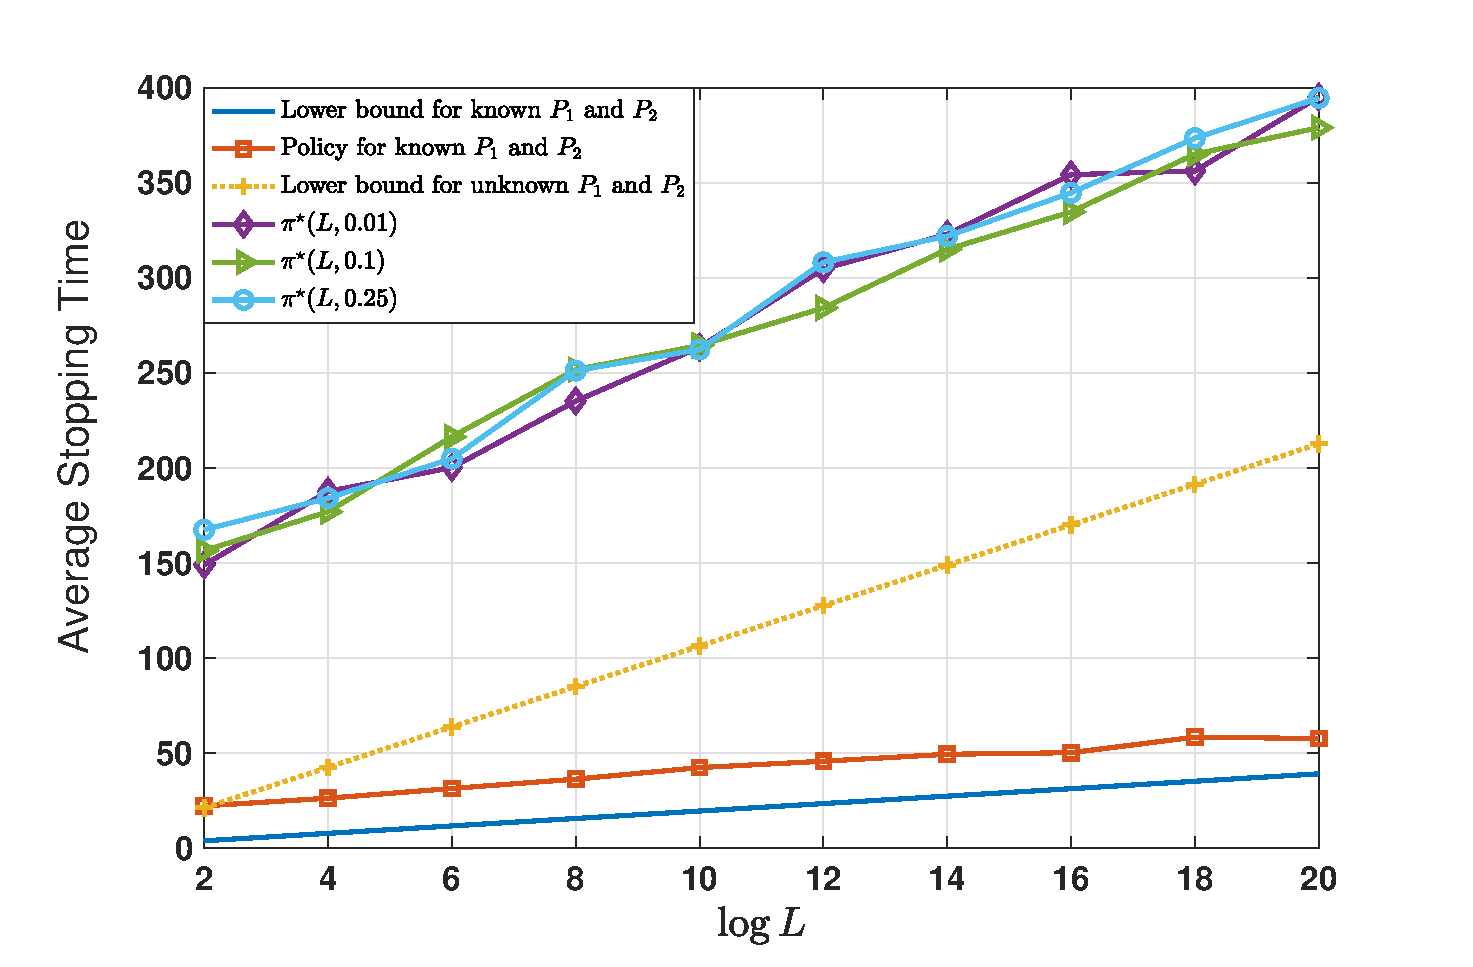
\includegraphics[width=11cm,height=7cm]{images/Plots8ArmsAndLmax20.eps}
	\end{center}
	\caption{Plots of average stopping time of policy $\pi^{\star}(L,\delta)$, as function of $\log L$, for $\delta=0.01,0.1,0.25$.}
	\label{rested_arms_fig:plots}
\end{figure}
Fix $K=8$ and $C=(h,P_1,P_2)$, with $h=1$ and $$ P_1=\begin{bmatrix}
	0.5&0.5\\0.5&0.5
\end{bmatrix},\quad  P_2=\begin{bmatrix}
	0.1&0.9\\0.9&0.1
\end{bmatrix}.$$
Fig. \ref{rested_arms_fig:plots} depicts the average stopping time of policy $\pi^{\star}(L,\delta)$ as a function of $\log L$, averaged over $100$ rounds of iterations, for $\delta=0.01,0.1,0.25$. For the aforementioned values of $P_1$ and $P_2$, numerical evaluation yields $D^*(h,P_1,P_2) \simeq 0.094$, thus resulting in a lower bound of $1/D^*(h,P_1,P_2) \simeq 10.635$. Since \eqref{rested_arms_eq:lower_bound} is a statement about the slope of the growth rate of average stopping time of policy $\pi^{\star}(L,\delta)$ as a function of $\log L$, the top 3 plots in the figure respect the lower bound in \eqref{rested_arms_eq:lower_bound}, with the slopes in these plots only marginally higher than that given by the lower bound. Theory predicts that as $\delta \downarrow 0$ and $L\to\infty$, the slopes will approach the lower bound. Also included in the figure are the plots of (a) the lower bound for the case when $P_1$ and $P_2$ are known, and (b) a policy similar to that of $\pi^{\star}(L,\delta)$ that uses the knowledge of $P_1$ and $P_2$ to identify the index of the odd arm. Such a policy clearly takes lesser time than $\pi^\star(L,\delta)$ to identify the index of the odd arm. The figure shows that the performance of this policy also matches in slope to that given by its lower bound for large values of $L$.

\section{Proofs}\label{rested_arms_sec:proofs_of_main_results}
\subsection{Proof of Proposition \ref{rested_arms_prop:lower_bound}}\label{rested_arms_appndx:proof_of_lower_bound}
We first present below three lemmas that will be used in proving the proposition. The first of these, given below, is an analogue of the change of measure argument of Kaufmann et al. \cite[Lemma 18]{kaufmann2016complexity} for the case of Markov observations from each arm. Recall that
\begin{equation*}
	\mathcal{F}_\tau=\{E\in\mathcal{F}:E\cap \{\tau=n\}\in\mathcal{F}_n\text{ for all }n\geq 0 \},	
\end{equation*}
where for each $n$, $\mathcal{F}_n$ is as defined in \eqref{rested_arms_eq:filtration}. Further, for any $h'\neq h$, define $Z_{hh'}(\tau)\coloneqq Z_{h}(\tau)-Z_{h'}(\tau)$, where $Z_{h}(\tau)=\sum_{a=1}^{K}Z_{h}^a(\tau)$.

\begin{lemma}\label{rested_arms_lemma:ChangeOfMeasure_htoh'}
	Fix $\epsilon>0$ and probability transition matrices $P_1$ and $P_2$, and let $\tau$ be the stopping time of a policy $\pi\in\Pi(\epsilon)$. Then, for any event $E\in \mathcal{F}_{\tau}$ and configuration triplets $C=(h,P_1,P_2)$ and $C'=(h',P_1',P_2')$, with $h'\neq h$, we have
	\begin{equation}
	P^\pi(E|C')=E^\pi[\mathbb{I}_{E}\,\,\exp(-Z_{hh'}(\tau))|C].\label{rested_arms_eq:statement_of_lemma_ChangeOfMeasure_htoh'}
	\end{equation}
\end{lemma}

\begin{proof}
The proof follows the outline in \cite{kaufmann2016complexity}, with crucial modifications needed for the Markov problem at hand. We use the shorthand notations $E_{h}[\cdot]$ and $E_{h'}[\cdot]$ to denote respectively the quantities $E^\pi[\cdot|C]$ and $E^\pi[\cdot|C']$; similarly, $P_{h}(\cdot)$ and $P_{h'}(\cdot)$ denote the respective probabilities. We begin by showing that for all $n\geq 0$, the following statement is true: for any measurable function $g:\mathcal{A}^{n+1}\times\mathcal{S}^{n+1}\to \mathbb{R}$, we have
\begin{equation}
E_{h'}[g(A^n,\bar{X}^{n})]=E_{h}[g(A^n,\bar{X}^{n})\,\exp(-Z_{hh'}(n))].\label{rested_arms_eq:for_all_g_mble_lemma}
\end{equation}
Assuming that the above statement is true, for any $E\in \mathcal{F}_{\tau}$, we have
\begingroup\allowdisplaybreaks\begin{align}
P_{h'}(E)&=E_{h'}[\mathbb{I}_{E}]\nonumber\\
&\stackrel{(a)}{=}\sum\limits_{n=0}^{\infty} E_{h'}[\mathbb{I}_{E}\mathbb{I}_{\{\tau=n\}}]\nonumber\\
&\stackrel{(b)}{=}\sum\limits_{n=0}^{\infty} E_{h}[\mathbb{I}_{E}\mathbb{I}_{\{\tau=n\}}\,\exp(-Z_{hh'}(n))]\nonumber\\
&=E_{h}[\mathbb{I}_{E}\,\,\exp(-Z_{hh'}(\tau))],\label{rested_arms_eq:proof_lem_1}
\end{align}\endgroup
hence proving the lemma. In the above set of equations, $(a)$ is due to monotone convergence theorem, and $(b)$ follows from the application of \eqref{rested_arms_eq:for_all_g_mble_lemma} to the function $g(A^n,\bar{X}^{n})=\mathbb{I}_{E}\cdot\mathbb{I}_{\{\tau=n\}}$ by noting that $E\in \mathcal{F}_{\tau}$, and therefore $E\cap\{\tau=n\}\in \mathcal{F}_{n}$ for all $n$.

We now proceed to prove \eqref{rested_arms_eq:for_all_g_mble_lemma} by induction on $n$.
%Noting that for each $a\in\mathcal{A}$, $X_0^a\sim \nu$ under hypotheses $H_h$ and $H_{h'}$, we have
%\begingroup\allowdisplaybreaks\begin{align}
%	E_{h'}[g(X_0^a)]&=\sum\limits_{i\in\mathcal{S}} g(i)\nu(i)=E_{h}[g(X_0^a)].\label{rested_arms_eq:induction_n=0_case}
%\end{align}\endgroup
From \eqref{rested_arms_eq:log_likelihood_under_hyp_h_and_h'} and  \eqref{rested_arms_eq:Z_{hh'}^a(n)}, it follows that $Z_{hh'}(0)=0$. Then, for any measurable function $g:\mathcal{A}^{n+1}\times \mathcal{S}^{n+1}\to\mathbb{R}$, the proof of \eqref{rested_arms_eq:for_all_g_mble_lemma} for $n=0$ follows from the following set of equations:
\begingroup\allowdisplaybreaks\begin{align}
	E_{h'}[g(A_0,\bar{X}_0)]
	&=\sum\limits_{a=1}^{K}\sum\limits_{i\in\mathcal{S}}P_{h'}(A_0=a)\cdot P_{h'}(\bar{X}_0=i|A_0=a)\cdot g(a,i)\nonumber\\
	&=\sum\limits_{a=1}^{K}\sum\limits_{i\in\mathcal{S}}P_{h'}(A_0=a)\cdot P_{h'}(X_0^a=i)\cdot g(a,i)\nonumber\\
	&=\sum\limits_{a=1}^{K}\sum\limits_{i\in\mathcal{S}}P_{h'}(A_0=a)\cdot \nu(i)\cdot g(a,i)\nonumber\\
	&\stackrel{(a)}{=}\sum\limits_{a=1}^{K}\sum\limits_{i\in\mathcal{S}}P_{h}(A_0=a)\cdot P_h(X_0^a=i)\cdot g(a,i)\nonumber\\
	&=E_h[g(A_0,\bar{X}_0)]\nonumber\\
	&=E_h[g(A_0,\bar{X}_0)\exp(-Z_{hh'}(0))],
\end{align}\endgroup
where in writing $(a)$, we use
\begin{itemize}
\item the fact that $P_h(A_0=a)=P_{h'}(A_0=a)$ since the manner in which $A_0$ is selected is not a function of either $h$ or $h'$. For instance, we may assume that each of the arms is picked once in the first $K$ time instants, and note that this does not affect the asymptotic performance of the policy. In such a case, $P_h(A_0=1)=1=P_{h'}(A_0=1)$.
\item the fact that $X_0^a\sim \nu$ under hypotheses $H_h$ and $H_{h'}$.
\end{itemize}
 %(such an assumption is not very restrictive since the manner of selecting $A_0$ does not affect the asymptotic analysis that is of main interest to us).
%$$P_{h'}(X_0^a=i|A_0=a)=P_h(X_0^a=i|A_0=a)=\nu(i)$$ for each $i\in\mathcal{S}$. Therefore, we have $E_h[g(Z_0)]=E_{h'}[g(Z_0)]$.	

We now assume that \eqref{rested_arms_eq:for_all_g_mble_lemma} holds for some positive integer $n$, and show that it also holds for $n+1$. By the law of iterated expectations, we have
\begingroup\allowdisplaybreaks\begin{align}
&E_{h'}[g(A^{n+1},\bar{X}^{n+1})]=E_{h'}\left[E_{h'}\left[g(A^{n+1},\bar{X}^{n+1})|A^n,\bar{X}^n\right]\right].\label{rested_arms_eq:induc_hyp_appl}
\end{align}\endgroup
Since the inner conditional expectation term on the right-hand side of \eqref{rested_arms_eq:induc_hyp_appl} is a measurable function of $(A^n,\bar{X}^n)$, using the induction hypothesis, we get
\begingroup\allowdisplaybreaks\begin{align}
& E_{h'}[g(A^{n+1},\bar{X}^{n+1})]\nonumber\\
& =E_{h}\left[E_{h'}\left[g(A^{n+1},\bar{X}^{n+1})|A^n,\bar{X}^n\right]\,\exp(-Z_{hh'}(n))\right]\nonumber\\
&=\sum\limits_{a^n\in\mathcal{A}^n}\sum\limits_{\bar{x}^n\in \mathcal{S}^{n+1}}P_h(A^n=a^n,\bar{X}^n=\bar{x}^n)\cdot \exp(-z_{hh'}(n))\cdot E_{h'}[g(A^{n+1},\bar{X}^{n+1})|A^n=a^n,\bar{X}^n=\bar{x}^n]\label{rested_arms_eq:lem_1_induc_partial_1},
\end{align}\endgroup
where $z_{hh'}(n)$ denotes the value of $Z_{hh'}(n)$ when $A^n=a^n$ and $\bar{X}^n=\bar{x}^n$. Then, we have
\begingroup\allowdisplaybreaks\begin{align}
&E_{h'}[g(A^{n+1},\bar{X}^{n+1})|A^n=a^n,\bar{X}^n=\bar{x}^n]\nonumber\\
&=\sum\limits_{a'=1}^{K}\sum\limits_{j\in\mathcal{S}}g(a^n,a',\bar{x}^n,j)\cdot P_{h'}(A_{n+1}=a'|A^n=a^n,\bar{X}^n=\bar{x}^n)
\cdot P_{h'}^{a'}(X_{N_{a'}(n)}^{a'}=j|X_{N_{a'}(n)-1}^{a'})\nonumber\\
&=\sum\limits_{a'=1}^{K}\sum\limits_{j\in\mathcal{S}}g(a^n,a',\bar{x}^n,j)\cdot P_{h}(A_{n+1}=a'|A^n=a^n,\bar{X}^n=\bar{x}^n)
\cdot P_{h'}^{a'}(X_{N_{a'}(n)}^{a'}=j|X_{N_{a'}(n)-1}^{a'}),\label{rested_arms_eq:lem_1_induc_partial_2}
\end{align}\endgroup
where in writing the last line above, we use the fact that the probability of selecting an arm at any time, based on the history of past arm selections and observations, is independent of the underlying configuration of the arms, and is thus the same under hypotheses $H_h$ and $H_{h'}$. We now write \eqref{rested_arms_eq:lem_1_induc_partial_2} as
\begingroup\allowdisplaybreaks\begin{align}
&E_{h'}[g(A^{n+1},\bar{X}^{n+1})|A^n=a^n,\bar{X}^n=\bar{x}^n]\nonumber\\
&=\sum\limits_{a'=1}^{K}\sum\limits_{j\in\mathcal{S}}\bigg\lbrace g(a^n,a',\bar{x}^n,j)\cdot P_{h}(A_{n+1}=a'|A^n=a^n,\bar{X}^n=\bar{x}^n)\nonumber\\
&\hspace{4cm}
\cdot\frac{P_{h'}^{a'}(X_{N_{a'}(n)-1}^{a'}=j|X_{N_{a'}(n)-1}^{a'})}{P_{h}^{a'}(X_{N_{a'}(n)}^{a'}=j|X_{N_{a'}(n)-1}^{a'})}\cdot P_{h}^{a'}(X_{N_{a'}(n)}^{a'}=j|X_{N_{a'}(n)-1}^{a'})\bigg\rbrace.\label{rested_arms_eq:lem_1_induc_partial_3}
\end{align}\endgroup
Plugging back \eqref{rested_arms_eq:lem_1_induc_partial_3} in \eqref{rested_arms_eq:lem_1_induc_partial_1}, and using
\begin{equation}
	z_{hh'}(n+1)=z_{hh'}(n)+\log\frac{P_{h}^{a'}(X_{N_{a'}(n)}^{a'}=j|X_{N_{a'}(n)-1}^{a'})}{P_{h'}^{a'}(X_{N_{a'}(n)}^a=j|X_{N_{a'}(n)-1}^{a'})},
\end{equation}
we get
\begingroup\allowdisplaybreaks\begin{align}
&E_{h'}[g(A^{n+1},\bar{X}^{n+1})]\nonumber\\
&=\sum\limits_{a^n\in\mathcal{A}^n}\sum\limits_{\bar{x}^n\in \mathcal{S}^{n+1}}\sum\limits_{a'=1}^{K}\sum\limits_{j\in\mathcal{S}}\bigg\lbrace g(a^n,a',\bar{x}^n,j)\cdot \exp(-z_{hh'}(n+1))\nonumber\\
&\hspace{3cm}\cdot P_h(A^n=a^n,\bar{X}^n=\bar{x}^n)
\cdot P_{h}(A_{n+1}=a',\bar{X}_{n+1}=j|A^n=a^n,\bar{X}^n=\bar{x}^n)\bigg\rbrace\nonumber\\
&=E_h[g(A^{n+1},\bar{X}^{n+1})\exp(-Z_{hh'}(n+1))],
\end{align}\endgroup
hence proving \eqref{rested_arms_eq:statement_of_lemma_ChangeOfMeasure_htoh'} .
%Now,
%\begingroup\allowdisplaybreaks\begin{align}
%&E_{h'}[g(A^{n+1},\bar{X}^{n+1}|\mathcal{F}_{n},A_{n+1}=a]\exp(-Z_{hh'}(n))
%&E_{h'}[g(A^n,a,\bar{X}^{n},X_{N_a(n)}^{a})|\mathcal{F}_{n},A_{n+1}=a]\cdot \exp(-Z_{hh'}(n))
%&=\sum\limits_{j\in S} g(A^n,a,\bar{X}^{n},j)\cdot \frac{P_{h'}^{a}(X_{N_a(n)}^{a}=j|X_{N_a(n)-1}^{a})}{P_{h}^{a}(X_{N_a(n)}^{a}=j|X_{N_a(n)-1}^{a})}
%&\hspace{2cm}\cdot P_{h}^{a}(X_{N_a(n)}^{a}=j|X_{N_a(n)-1}^{a})\cdot \exp(-Z_{hh'}(n))
%&=\sum\limits_{j\in\mathcal{S}}g(A^n,a,\bar{X}^{n},j)\cdot P_{h}^{a}(X_{N_a(n)}^{a}=j|X_{N_a(n)-1}^{a})
%&\hspace{4cm}\cdot \exp(-Z_{hh'}(n+1))\label{rested_arms_eq:lem_1_induc_partial_2}
%\end{align}\endgroup
%Plugging in \eqref{rested_arms_eq:lem_1_induc_partial_2} into \eqref{rested_arms_eq:lem_1_induc_partial_1}, we get
%\begingroup\allowdisplaybreaks\begin{align}
%&E_{h'}[g(Z^{n+1})]
%&\stackrel{(a)}{=}E_{h}\bigg[\sum\limits_{a=1}^{K}\sum\limits_{j\in S}\mathbb{I}_{\{A_{n+1}=a\}}g(Z^{n},j)
%&\hspace{1cm}P_{h}^{a}(X_{N_a(n)}^a=j|X_{N_a(n)-1}^a)\exp(-Z_{hh'}^a(n+1,j))\bigg\vert\mathcal{F}_n\bigg]
%&=E_{h}\bigg[E_h[g(Z^{n+1})\,\exp\left(-Z_{hh'}(n+1)\right)|\mathcal{F}_{n}]\bigg]
%&=E_h[g(Z^{n+1})\,\exp\left(-Z_{hh'}(n+1)\right)],\label{rested_arms_eq:lem_1_induc_partial_3}
%\end{align}\endgroup
%where in $(a)$ above,
%\begingroup\allowdisplaybreaks\begin{align}
%&Z_{hh'}^a(n+1,j)
%&\coloneqq\sum\limits_{a=1}^{K}\sum\limits_{m=1}^{N_{a}(n)-1}\log\left(\frac{P_{h}^{a}(X_m^{a}|X_{m-1}^{a})}{P_{h'}^{a}(X_{m}^{a}|X_{m-1}^{a})}\right)
%
%&\hspace{2cm}+\log\left(\frac{P_{h}^{a}(X_{N_a(n)}^a=j|X_{N_a(n)-1}^a)}{P_{h'}^{a}(X_{N_a(n)}^a=j|X_{N_a(n)-1}^a)}\right).
%\end{align}\endgroup
\end{proof}

The second lemma below relates the expected number of $i$ to $j$ transitions $E^\pi[N_a(\tau,i,j)|C]$ observed on the Markov process of arm $a$ to $E^\pi[N_a(\tau,i)|C]$, the expected number of exits out of state $i$ observed on the Markov process of arm $a$.

\begin{lemma}\label{rested_arms_lemma:RelBtwNijAndNi}
	Fix $\epsilon>0$, a policy $\pi\in\Pi(\epsilon)$, and a configuration $C=(h,P_1,P_2)$. For each $i,j\in \mathcal{S}$ and $a\in \mathcal{A}$, we have
	\begin{equation}
	E^\pi[N_a(\tau,i,j)|C]=E^\pi[N_a(\tau,i)|C]\cdot P_{h}^a(j|i),\label{rested_arms_eq:RelBtwNijAndNi}
	\end{equation}
	where $P_h^a(j|i)$ is as given in \eqref{rested_arms_eq:P_h^a(j|i)}.
	\qed
\end{lemma}

\begin{proof}
We use the shorthand notation $E_h[\cdot]$ to denote $E^\pi[\cdot|C]$.
We demonstrate that for each $i,j\in \mathcal{S}$ and $a\in \mathcal{A}$,
\begingroup\allowdisplaybreaks\begin{align}
{E}_{h}[{E}_{h}[N_a(\tau,i,j)|X_0^a]|N_a(\tau)]
=E_{h}[E_{h}[N_a(\tau,i)|X_0^a]|N_a(\tau)]\cdot P_h^a(j|i).\label{rested_arms_eq:RelBtwNijAndNiWithIteratedExpec}
\end{align}\endgroup
Towards this, we note that
\begingroup\allowdisplaybreaks\begin{align}
E_{h}[E_{h}[N_a(\tau,i,j)|X_0^a]|N_a(\tau)]
=E_{h}\left[\sum\limits_{m=1}^{N_a(\tau)-1}E_{h}[\mathbb{I}_{\{X_{m-1}^a=i,\,X_m^a=j\}}|X_0^a]\bigg\vert N_a(\tau)\right].\label{rested_arms_eq:lower_bound_partial_5_rested_arms}
\end{align}\endgroup
We now simplify the inner conditional expectation term in \eqref{rested_arms_eq:lower_bound_partial_5_rested_arms} by considering the cases $m=1$ and $m\geq 2$ separately.
\begin{enumerate}
	\item Case $m=1$:
	In this case, we get
	\begingroup\allowdisplaybreaks\begin{align}
	E_{h}[\mathbb{I}_{\{X_{0}^a=i,\,X_1^a=j\}}|X_0^a]
	&=\mathbb{I}_{\{X_{0}^a=i\}}\cdot E_{h}[\mathbb{I}_{\{X_1^a=j\}}|X_0^a]\nonumber\\
	&=\mathbb{I}_{\{X_{0}^a=i\}}\cdot P_h^a(X_1^a=j|X_0^a=i)\nonumber\\
	&=\mathbb{I}_{\{X_{0}^a=i\}}\cdot P_h^a(j|i).\label{rested_arms_eq:Casem=1}
	\end{align}\endgroup
	\item Case $m\geq 2$: Here, we get
	\begingroup\allowdisplaybreaks\begin{align}
	E_{h}[\mathbb{I}_{\{X_{m-1}^a=i,\,X_m^a=j\}}|X_0^a=k]
	&=P_h^a(X_{m-1}^a=i,\,X_m^a=j|X_0^a=k)\nonumber\\
	&\stackrel{(a)}{=}P_h^a(X_{m-1}^a=i|X_0^a=k)\cdot P_h^a(X_1^a=j|X_0^a=i)\nonumber\\
	&=E_{h}[\mathbb{I}_{\{X_{m-1}^{a}=i\}}|X_0^a=k]\cdot P_h^a(j|i),
	\end{align}\endgroup
	from which it follows that $E_{h}[\mathbb{I}_{\{X_{m-1}^a=i,\,X_m^a=j\}}|X_0^a]=E_{h}[\mathbb{I}_{\{X_{m-1}^{a}=i\}}|X_0^a]\cdot P_h^a(j|i)$. In the above set of equations, $(a)$ follows from the fact that the Markov process of arm $a$ is time homogeneous.
\end{enumerate}
From the aforementioned cases, it follows that the relation
\begingroup\allowdisplaybreaks\begin{align}
E_{h}[\mathbb{I}_{\{X_{m-1}^a=i,\,X_m^a=j\}}|X_0^a]=E_{h}[\mathbb{I}_{\{X_{m-1}^{a}=i\}}|X_0^a]\cdot P_h^a(j|i)\label{rested_arms_eq:ConditioningOnX_0^a}
\end{align}\endgroup
holds for all $m\geq 1$. Substituting \eqref{rested_arms_eq:ConditioningOnX_0^a} in \eqref{rested_arms_eq:lower_bound_partial_5_rested_arms} and simplifying, we arrive at \eqref{rested_arms_eq:RelBtwNijAndNiWithIteratedExpec}. The lemma then follows by applying expectation $E_{h}[\cdot]$ to both sides of \eqref{rested_arms_eq:RelBtwNijAndNiWithIteratedExpec}.	
\end{proof}

The third lemma presented below will be used to simplify a minimisation term later in the proof of the proposition.
 \begin{lemma}
 \label{rested_arms_lemma:convex_comb_of_KL_div}
% 	Denote by $\mathcal{P}(\mathcal{S})$ the set of all probability distributions on the set $\mathcal{S}$, and let $\nu_1$ and $\nu_2$ be any two distinct elements of $\mathcal{P}(\mathcal{S})$. Then, 
	For all $w_1,w_2\in[0,1]$ such that $w_1+w_2=1$ and $\nu_1, \nu_2\in \mathcal{P}(\mathcal{S})$, 
 	\begingroup\allowdisplaybreaks\begin{align}
 		\min\limits_{\psi\in\mathcal{P}(\mathcal{S})}\left[w_1 D(\nu_1||\psi)+w_2 D(\nu_2||\psi)\right]
 		=w_1 D(\nu_1||\nu^*)+w_2 D(\nu_2||\nu^*),\label{rested_arms_eq:convex_comb_of_KL_div}
 	\end{align}\endgroup
 	where $\nu^*\in\mathcal{P}(\mathcal{S})$ is given by $\nu^*=w_1\nu_1+w_2\nu_2$.
 \end{lemma}
 \begin{proof}
 This is well known with $\nu^*$ viewed as a root of ``information centre'' and the right-hand side of \eqref{rested_arms_eq:convex_comb_of_KL_div} viewed as a mutual information. Here is the proof for completeness.

  Let $\nu^*$ be as defined in the statement of the lemma. For any $\psi\in\mathcal{P}(\mathcal{S})$, we have
{\color{black}
 \begingroup\allowdisplaybreaks\begin{align}
 w_1 D(\nu_1||\psi)+w_2 D(\nu_2||\psi)
% &=w_1E_{\nu_1}\left[\log\frac{d\nu_1}{d\psi}\right]+w_2E_{\nu_2}\left[\log\frac{d\nu_2}{d\psi}\right]\nonumber\\
% &=w_1E_{\nu_1}\left[\log\frac{d\nu_1}{d\nu^*}\right]+w_2E_{\nu_2}\left[\log\frac{d\nu_2}{d\nu^*}\right]+w_1E_{\nu_1}\left[\log\frac{d\nu^*}{d\psi}\right]+w_2E_{\nu_2}\left[\log\frac{d\nu^*}{d\psi}\right]\nonumber\\
% &=w_1E_{\nu_1}\left[\log\frac{d\nu_1}{d\nu^*}\right]+w_2E_{\nu_2}\left[\log\frac{d\nu_2}{d\nu^*}\right]+E_{\nu^*}\left[\log\frac{d\nu^*}{d\psi}\right]\nonumber\\
 &=w_1D(\nu_1\|\nu^*)+w_2 D(\nu_2\| \nu^*)+D(\nu^*||\psi)\nonumber\\
 &\geq D(\nu_1\|\nu^*)+w_2 D(\nu_2\| \nu^*),\label{rested_arms_eq:conv_comb_of_KL_div_proof}
 \end{align}\endgroup}
 with equality in the last line above if and only if $\psi=\nu^*$. This completes the proof of the lemma.	
 \end{proof}

\begin{proof}[Proof of Proposition \ref{rested_arms_prop:lower_bound}]
Fix an arbitrary $\epsilon>0$, and let $\pi\in\Pi(\epsilon)$ be a policy whose stopping is $\tau=\tau(\pi)$. Without loss of generality, we assume that $E^\pi[\tau(\pi)|C] < \infty$, for otherwise the inequality \eqref{rested_arms_eq:lower_bound} holds trivially. We organise the proof of the proposition into various sections. In the first of these sections presented below, we lower bound the expected value of $Z_{hh'}(\tau)$ in terms of the error probability $\epsilon$. This uses the above Lemma \ref{rested_arms_lemma:ChangeOfMeasure_htoh'}, Lemma \ref{rested_arms_lemma:RelBtwNijAndNi} and the result of \cite[Lemma 19]{kaufmann2016complexity}.

\subsubsection{A Lower Bound on The Expected Value of $Z_{hh'}(\tau)$}
Let $\pi\in\Pi(\epsilon)$, with stopping time is $\tau=\tau(\pi)$. For any $h'\neq h$, let $Z_{hh'}(\tau)$ be as defined in the statement of Lemma \ref{rested_arms_lemma:ChangeOfMeasure_htoh'}. Then, Lemma \ref{rested_arms_lemma:ChangeOfMeasure_htoh'} in conjunction with \cite[Lemma 19]{kaufmann2016complexity} yields the following: conditioned on the underlying configuration $C=(h,P_1,P_2)$, for any alternative configuration $C'=(h',P_1',P_2')$, where $h'\neq h$, under the assumption that $E^\pi[\tau|C]<\infty$, we have
\begin{equation}
E^\pi[Z_{hh'}(\tau)|C]\geq \sup\limits_{E\in \mathcal{F}_{\tau}}d(P^\pi(E|C),P^\pi(E|C')),\label{rested_arms_eq:analog_of_lemma_19_Kaufmann}
\end{equation}
 where \[d(p,q)\coloneqq p\log\left(\frac{p}{q}\right)+(1-p)\log\left(\frac{1-p}{1-q}\right)\]
denotes the binary KL divergence, with the convention that $d(0,0)=0=d(1,1)$. We now note the following points:
\begin{enumerate}
    \item For each alternative configuration $C'$, by taking $E=\{I(\pi)=h\}$ and recognising that $\pi\in\Pi(\epsilon)$, we have $P^\pi(E|C)>1-\epsilon$ and $P^\pi(E|C')\leq \epsilon$. Using this, along with the fact that the mapping $x\mapsto d(x,y)$ is monotone increasing for $x<y$ and the mapping $y\mapsto d(x,y)$ is monotone decreasing for any fixed $x$, we obtain
	\begingroup\allowdisplaybreaks\begin{align}
		d(P^\pi(E|C),P^\pi(E|C'))&\geq d(1-\epsilon,P^\pi(E|C'))\nonumber\\
		&\geq d(1-\epsilon,\epsilon).
	\end{align}\endgroup
	
	\item We may minimise both sides of \eqref{rested_arms_eq:analog_of_lemma_19_Kaufmann} over all alternative configurations $C'$ to obtain
	\begingroup\allowdisplaybreaks\begin{align}
		\min\limits_{C'=(h',P_1',P_2')}E^\pi[Z_{hh'}(\tau)|C]
		\geq \min\limits_{C'=(h',P_1',P_2')}\,\sup\limits_{E\in \mathcal{F}_{\tau}}d(P^\pi(E|C),P^\pi(E|C')).\label{rested_arms_eq:analog_of_lemma_19_Kaufmann_min_over_all_C'}
	\end{align}\endgroup
\end{enumerate}

Combining the points noted above, and using $d(1-\epsilon,\epsilon)=d(\epsilon,1-\epsilon)$, we obtain
\begin{equation}
\min\limits_{C'=(h',P_1',P_2')}{E}^\pi[Z_{hh'}(\tau)|C]\geq d(\epsilon,1-\epsilon).\label{rested_arms_eq:lower_bound_partial_1}
\end{equation}

\subsubsection{A Relation Between $E^\pi[Z_{hh'}(\tau)|C]$ and $E^\pi[\tau|C]$}
 As our next step, we obtain an upper bound for $E^\pi[Z_{hh'}(\tau)|C]$ in terms of $E^\pi[\tau|C]$. Towards this, we have
\begingroup\allowdisplaybreaks\begin{align}
{E}^\pi[Z_{hh'}(\tau)|C]
%\sum\limits_{a=1}^{K}{E}^\pi\bigg[\log\left(\frac{P_h^{a}(X_{0}^{a})}{P_{h'}^{a}(X_{0}^{a})}\right)\bigg\vert C\bigg]
=\sum\limits_{a=1}^{K}{E}^\pi\bigg[\sum\limits_{m=1}^{N_{a}(\tau)-1}\log\left(\frac{P_{h}^{a}(X_{m}^{a}|X_{m-1}^{a})}{P_{h'}^{a}(X_{m}^{a}|X_{m-1}^{a})}\right)\bigg\vert C\bigg],\label{rested_arms_eq:lower_bound_partial_2_rested}
\end{align}\endgroup
where we take inner summation term to be zero whenever $N_a(\tau)<2$.
Focus on the expectation term in \eqref{rested_arms_eq:lower_bound_partial_2_rested}.
%and note that for each $a\in \mathcal{A}$.
This term may be written as
\begingroup\allowdisplaybreaks\begin{align}
E^\pi\bigg[\sum\limits_{m=1}^{N_{a}(\tau)-1}\log\left(\frac{P_{h}^{a}(X_{m}^{a}|X_{m-1}^{a})}{P_{h'}^{a}(X_{m}^{a}|X_{m-1}^{a})}\right)\bigg\vert C\bigg]
%            &=E_{h}\bigg[\sum\limits_{m=1}^{N_{a}(\tau)-1}\sum\limits_{i,j\in S}\mathbb{I}_{\{X_{m-1}^a=i,\,X_m^a=j\}} \log\left(\frac{P_{h}^{a}(X_{m}^{a}=j|X_{m-1}^{a}=i)}{P_{h'}^{a}(X_{m}^{a}=j|X_{m-1}^{a}=i)}\right)\bigg]
&\stackrel{(a)}{=}E^\pi\bigg[\sum\limits_{m=1}^{N_{a}(\tau)-1}\sum\limits_{i,j\in S}\mathbb{I}_{\{X_{m-1}^a=i,\,X_m^a=j\}}\log\left(\frac{P_{h}^{a}(j|i)}{P_{h'}^{a}(j|i)}\right)\bigg\vert C\bigg]\nonumber\\
&=\sum\limits_{i,j\in S}E^\pi[N_a(\tau,i,j)|C]\,f^a_{hh'}(j|i),\label{rested_arms_eq:lower_bound_partial_3_rested_bandit}
\end{align}\endgroup
where $(a)$ above follows from the fact that the Markov process of arm $a$ is time homogeneous, and $f_{hh'}^a(j|i)\coloneqq\log\left(\frac{P_{h}^{a}(j|i)}{P_{h'}^{a}(j|i)}\right)$. Using the result of Lemma \ref{rested_arms_lemma:RelBtwNijAndNi} in \eqref{rested_arms_eq:lower_bound_partial_3_rested_bandit}, we get
\begingroup\allowdisplaybreaks\begin{align}
E^\pi[Z_{hh'}(\tau)|C]
&=\sum\limits_{a=1}^{K}\,\sum\limits_{i,j\in S}{E}^\pi[N_a(\tau,i)|C]\cdot P_{h}^a(j|i)\cdot f^a_{hh'}(j|i)\nonumber\\
&=\sum\limits_{a=1}^{K}\,\sum\limits_{i\in S}{E}[N_a(\tau,i)|C]\,D(P_h^a(\cdot|i)||P_{h'}^a(\cdot|i)),\label{rested_arms_eq:lower_bound_partial_6_rested_arms}
\end{align}\endgroup
where $D(P_h^a(\cdot|i)||P_{h'}^a(\cdot|i))=\sum\limits_{j\in S}P_{h}^a(j|i)f^a_{hh'}(j|i)$ denotes the KL divergence between the probability distributions $P_h^a(\cdot|i)$ and $P_{h'}^a(\cdot|i)$. We now express \eqref{rested_arms_eq:lower_bound_partial_6_rested_arms} by introducing some additional terms as below:
\begingroup\allowdisplaybreaks\begin{align}
&E^\pi[Z_{hh'}(\tau)|C]\nonumber\\
&=(E^\pi[\tau+1|C]-K)
\bigg(\sum\limits_{a=1}^{K}\bigg[\frac{E^\pi[N_a(\tau)|C]-1}{E^\pi[\tau+1|C]-K}\bigg]\sum\limits_{i\in \mathcal{S}}\bigg[\frac{E^\pi[N_a(\tau,i)|C]}{E^\pi[N_a(\tau)|C]-1}\bigg]
D(P_h^a(\cdot|i)||P_{h'}^a(\cdot|i))\bigg)\nonumber\\
&=(E^\pi[\tau+1|C]-K)\bigg(\sum\limits_{a=1}^{K}\bigg[\frac{E^\pi[N_a(\tau)|C]-1}{E^\pi[\tau+1|C]-K}\bigg]
\sum\limits_{i\in \mathcal{S}}p_h^a(i)\cdot D(P_h^a(\cdot|i)||P_{h'}^a(\cdot|i))\bigg),\label{rested_arms_eq:lower_bound_partial_7_rested_arms}
\end{align}\endgroup
where $p_h^a(i)\coloneqq\frac{E^\pi[N_a(\tau,i)|C]}{E^\pi[N_a(\tau)|C]-1}$ represents the average (computed with respect to $E^\pi[\cdot|C])$ fraction of times a transition {out} of state $i$ is observed on the Markov process of arm $a$.

\subsubsection{Asymptotics of Vanishing Error Probability}
Since $\sum\limits_{i\in \mathcal{S}}p_h^a(i)=1$, the inner summation term over $i$ in \eqref{rested_arms_eq:lower_bound_partial_7_rested_arms} represents the average of the numbers $(D(P_h^a(\cdot|i)||P_{h'}^a(\cdot|i)))_{i\in \mathcal{S}}$ with respect to $(p_h^a(i))_{i\in \mathcal{S}}$. Suppose that at some time, arm $a$ is selected, and it \textcolor{black}{makes a transition from state $i$ to state $j$}, for some $i,j\in \mathcal{S}$. Then, the next time arm $a$ is selected, it \textcolor{black}{makes a transition from state $j$ to state $k$} for some $k\in \mathcal{S}$. For $a\in \mathcal{A}$ and $i\in \mathcal{S}$, let
\begin{equation}
N^a(\tau,i)\coloneqq\sum\limits_{m=2}^{N_a(\tau)}\mathbb{I}_{\{X_{m-1}^a=i\}}\label{rested_arms_eq:NoOfEntriesIntoStatei}
\end{equation}
denote the number of times arm $a$ \textcolor{black}{is observed to occupy state $i$ after a transition}. In conjunction with \eqref{rested_arms_eq:N_a(n,i)}, it is easy to see that for each $i\in \mathcal{S}$, we have
\begin{equation}
N_a(\tau,i)=N^a(\tau,i)-\mathbb{I}_{\{X_{N_a(\tau)-1}^a=i\}}+\mathbb{I}_{\{X_0^a=i\}},\label{rested_arms_eq:RelBtwEntryAndExitNumbersForStatei}
\end{equation}
which implies that $N^a(\tau,i)-1\leq N_a(\tau,i)\leq N^a(\tau,i)+1$ \text{almost surely} Thus, we notice that for the Markov process of each arm, for each $i\in\mathcal{S}$, \textcolor{black}{the number of times the arm is observed to occupy state $i$ prior to a transition is at most one more than the number of times it is observed to occupy state $i$ after a transition}.  We then have
\begin{equation}
\frac{E^\pi[N^a(\tau,i)|C]-1}{E^\pi[N_a(\tau)|C]-1}\leq p_h^a(i)\leq \frac{E^\pi[N^a(\tau,i)|C]+1}{E^\pi[N_a(\tau)|C]-1}.\label{rested_arms_eq:p_h^a_in_limit}
\end{equation}

Using \eqref{rested_arms_eq:p_h^a_in_limit} in \eqref{rested_arms_eq:lower_bound_partial_7_rested_arms}, we arrive at the form
\begingroup\allowdisplaybreaks\begin{align}
	u-\Delta\leq E^\pi[Z_{hh'}(\tau)]
	\leq u+\Delta,\label{rested_arms_eq:lower_bound_partial_8}
\end{align}\endgroup
where the terms $u$ and $\Delta$ are as below:
\begingroup\allowdisplaybreaks\begin{align}
u&=(E^\pi[\tau+1|C]-K)
\bigg(\sum\limits_{a=1}^{K}\bigg[\frac{E^\pi[N_a(\tau)|C]-1}{E^\pi[\tau+1|C]-K}\bigg]
\sum\limits_{i\in \mathcal{S}}\bigg[\frac{E^\pi[N^a(\tau,i)|C]}{E^\pi[N_a(\tau)|C]-1}\bigg] D(P_h^a(\cdot|i)||P_{h'}^a(\cdot|i))\bigg),\nonumber\\
\Delta &=\sum\limits_{a=1}^{K}\sum\limits_{i\in\mathcal{S}}D(P_h^a(\cdot|i)||P_{h'}^a(\cdot|i))
=\sum\limits_{i\in\mathcal{S}}D(P_1(\cdot|i)||P_2'(\cdot|i))+\sum\limits_{i\in\mathcal{S}}D(P_2(\cdot|i)||P_1'(\cdot|i))
\nonumber\\
&\hspace{9cm}+\sum\limits_{a\neq h}\sum\limits_{i\in\mathcal{S}}D(P_2(\cdot|i)||P_2'(\cdot|i)).
\end{align}\endgroup

We shall soon show that the regime of vanishing error probabilities, i.e., $\epsilon\downarrow 0$, necessarily means that for each $a\in\mathcal{A}$, $E^\pi[N_a(\tau)|C]\to \infty$, which in turn implies that $E^\pi[\tau|C]\to\infty$. In this asymptotic regime, for each $a\in\mathcal{A}$, the limiting probabilities of \textcolor{black}{arm $a$ occupying a state $i\in \mathcal{S}$ prior to and after a transition are equal, and invariant to the one step transitions on arm $a$}. Since the Markov process of arm $a$ is irreducible and positive recurrent, its probability transition matrix admits a unique stationary distribution. Therefore, by the Ergodic theorem, the aforementioned probabilities must converge to those given by the stationary distribution associated with arm $a$. We shall denote this stationary distribution by $\mu_h^a(\cdot)$ under configuration $C=(h,P_1,P_2)$, given by
\begin{equation}
	\mu_h^a(i)=\begin{cases}
		\mu_1(i),&a=h,\\
		\mu_2(i),&a\neq h.
	\end{cases}\label{rested_arms_eq:mu_h^a}
\end{equation}
Then, as $\epsilon\downarrow 0$, we have that both the lower and upper bounds in \eqref{rested_arms_eq:p_h^a_in_limit} converge to $\mu_h^a(i)$ . We shall soon exploit this fact below to arrive at the lower bound. Going further, we denote by $(q_h^a(i))_{i\in\mathcal{S}}$ the probability distribution given by
\begin{equation}
q_h^a(i)=\frac{E^\pi[N^a(\tau,i)|C]}{E^\pi[N_a(\tau)|C]-1},\quad i\in\mathcal{S}.\label{rested_arms_eq:q_h^a}	
\end{equation}

Using the upper bound in \eqref{rested_arms_eq:lower_bound_partial_8} in combination with \eqref{rested_arms_eq:lower_bound_partial_1}, we have the following chain of inequalities:
\begingroup\allowdisplaybreaks\begin{align}
d(\epsilon,1-\epsilon)
&\leq\min\limits_{C'=(h',P_1',P_2')}\,{E}^\pi[Z_{hh'}(\tau)|C]\nonumber\\
&\leq \min\limits_{C'=(h',P_1',P_2')}(u+\Delta)\nonumber\\
&\leq \min\limits_{C'=(h',P_1',P_2')} u+\min\limits_{C'=(h',P_1',P_2')} \Delta.\label{rested_arms_eq:lower_bound_partial_9_rested_arms}
\end{align}\endgroup

The first term in \eqref{rested_arms_eq:lower_bound_partial_9_rested_arms} may be upper bounded as follows:
{\color{black}
\begingroup\allowdisplaybreaks\begin{align}
&\min\limits_{C'=(h',P_1',P_2')}u \nonumber\\
&	
%&=(E^\pi[\tau+1|C]-K)\,\bigg\lbrace\min\limits_{C'=(h',P_1',P_2')}\bigg(\sum\limits_{a=1}^{K}\bigg[\frac{E^\pi[N_a(\tau)|C]-1}{E^\pi[\tau+1|C]-K}\bigg]
%\sum\limits_{i\in \mathcal{S}}\bigg[\frac{E^\pi[N^a(\tau,i)|C]}{E^\pi[N_a(\tau)|C]-1}\bigg] D(P_h^a(\cdot|i)||P_{h'}^a(\cdot|i))\bigg)\bigg\rbrace\nonumber\\
= (E^\pi[\tau+1|C]-K)\,\bigg\lbrace
\min\limits_{C'=(h',P_1',P_2')}\bigg(\sum\limits_{a=1}^{K}\bigg[\frac{E^\pi[N_a(\tau)|C]-1}{E^\pi[\tau+1|C]-K}\bigg]\sum\limits_{i\in\mathcal{S}}q_h^a(i)\, D(P_h^a(\cdot|i)||P_{h'}^a(\cdot|i))\bigg)\bigg\rbrace\nonumber\\
&\stackrel{(a)}{=} (E^\pi[\tau+1|C]-K)\,\bigg\lbrace
\min\limits_{C'=(h',P_1',P_2')}\bigg(\sum\limits_{a=1}^{K}\bigg[\frac{E^\pi[N_a(\tau)|C]-1}{E^\pi[\tau+1|C]-K}\bigg]
 D(P_h^a(\cdot|\cdot)||P_{h'}^a(\cdot|\cdot)|q_h^a)\bigg)\bigg\rbrace\nonumber\\
&\stackrel{(b)}{\leq} (E^\pi[\tau+1|C]-K)\,\bigg\lbrace\max\limits_{\lambda\in\mathcal{P}(\mathcal{A})}\min\limits_{C'=(h',P_1',P_2')}\bigg(\sum\limits_{a=1}^{K}\lambda(a) D(P_h^a(\cdot|\cdot)||P_{h'}^a(\cdot|\cdot)|q_h^a)\bigg)\bigg\rbrace,\label{rested_arms_eq:proof_of_prop_1_temp_1}
\end{align}\endgroup}
where, in $(a)$ above,
\begin{align*}
D(P_h^a(\cdot|\cdot)||P_{h'}^a(\cdot|\cdot)|q_h^a)\coloneqq \sum\limits_{i\in S}q_h^a(i)\cdot D(P_h^a(\cdot|i)||P_{h'}^a(\cdot|i)),
\end{align*}
while $(b)$ follows by noting that maximising over the set $\mathcal{P}(\mathcal{A})$ of all probability distributions on the set of arms $\mathcal{A}$ only increases the right-hand side. The second term in \eqref{rested_arms_eq:lower_bound_partial_9_rested_arms} may be simplified as
\begingroup\allowdisplaybreaks\begin{align}
	&\min\limits_{C'=(h',P_1',P_2')}\Delta\nonumber\\
	&=\min\limits_{P_1',P_2':P_1'\neq P_2'}\bigg\lbrace \sum\limits_{i\in\mathcal{S}}D(P_1(\cdot|i)||P_2'(\cdot|i))+\sum\limits_{i\in\mathcal{S}}D(P_2(\cdot|i)||P_1'(\cdot|i))
+\sum\limits_{a\neq h}\sum\limits_{i\in\mathcal{S}}D(P_2(\cdot|i)||P_2'(\cdot|i))\bigg\rbrace\nonumber\\
&\stackrel{(a)}{=}\min\limits_{P_2'}\bigg\lbrace \sum\limits_{i\in\mathcal{S}}D(P_1(\cdot|i)||P_2'(\cdot|i))+\sum\limits_{a\neq h}\sum\limits_{i\in\mathcal{S}}D(P_2(\cdot|i)||P_2'(\cdot|i))\bigg\rbrace\nonumber\\
&=\min\bigg\lbrace\sum\limits_{i\in\mathcal{S}}D(P_1(\cdot|i)||P_2(\cdot|i)),~(K-1)\sum\limits_{i\in\mathcal{S}}D(P_2(\cdot|i)||P_1(\cdot|i))\bigg\rbrace,\label{rested_arms_eq:lower_bound_partial_10_rested_arms}
\end{align}\endgroup
where $(a)$ above follows by noting that $P_1'$ appears only in the term $D(P_2(\cdot|i)||P_1'(\cdot|i))$, and that for the choice $P_1'=P_2$, we get $D(P_2(\cdot|i)||P_1'(\cdot|i))=0$ for all $i\in\mathcal{S}$. For ease of notation, we shall denote the quantity in \eqref{rested_arms_eq:lower_bound_partial_10_rested_arms} by $\Delta'$, which we note is a constant.

Combining \eqref{rested_arms_eq:proof_of_prop_1_temp_1} with \eqref{rested_arms_eq:lower_bound_partial_9_rested_arms}, we get the following relation after rearrangement:
\begingroup\allowdisplaybreaks\begin{align}
	d(\epsilon,1-\epsilon)
	\leq \Delta' + (E^\pi[\tau+1|C]-K)\,\bigg\lbrace\max\limits_{\lambda\in\mathcal{P}(\mathcal{A})}\min\limits_{C'=(h',P_1',P_2')}\bigg[\sum\limits_{a=1}^{K}\lambda(a) D(P_h^a(\cdot|\cdot)||P_{h'}^a(\cdot|\cdot)|q_h^a)\bigg]\bigg\rbrace.\label{rested_arms_eq:proof_of_prop_1_temp_2}
\end{align}\endgroup

Since \eqref{rested_arms_eq:proof_of_prop_1_temp_2} is valid for any arbitrary choice of $\epsilon>0$ and for all $\pi\in\Pi(\epsilon)$, letting $\epsilon\downarrow 0$ and using $d(\epsilon,1-\epsilon)/\log \frac{1}{\epsilon} \to 1$ as $\epsilon\downarrow 0$, along with the fact that $q_h^a(i)\to \mu_h^a(i)$ for all $i\in\mathcal{S}$ in the regime of vanishing error probabilities, we get
 \begin{equation}
\lim\limits_{\epsilon\downarrow 0}\inf\limits_{\pi\in\Pi(\epsilon)}\frac{E^\pi[\tau(\pi)|C]}{\log\frac{1}{\epsilon}}\geq \frac{1}{D^*(h,P_1,P_2)},
\end{equation}
 	where the quantity $D^*(h,P_1,P_2)$ depends on the underlying configuration of the arms, and is given by
 	\begingroup\allowdisplaybreaks\begin{align}
 D^*(h,P_1,P_2)
=\max\limits_{\lambda\in\mathcal{P}(\mathcal{A})}\,\min\limits_{C'=(h',P_1',P_2')}\bigg(\sum\limits_{a=1}^{K}\lambda(a)\,D(P_h^a(\cdot|\cdot)||P_{h'}^a(\cdot|\cdot)|\mu_h^a)\bigg).\label{rested_arms_eq:D^*(h,P_1,P_2)}
 	\end{align}\endgroup
 	
We now show that the quantities in \eqref{rested_arms_eq:D^*(h,P_1,P_2)} and \eqref{rested_arms_eq:D^*(h,P_1,P_2)_simpl_final} are the same.
 	
\subsubsection{The Final Steps}
\label{rested_arms_subsec:final_steps}
 Using \eqref{rested_arms_eq:P_h^a(j|i)} and \eqref{rested_arms_eq:mu_h^a}, and using the shorthand notation $D(P_h^a||P_{h'}^a|\mu_h^a)$ to denote the KL divergence term inside the summation in \eqref{rested_arms_eq:D^*(h,P_1,P_2)}, we get
  \begingroup\allowdisplaybreaks\begin{align}
 		&D^*(h,P_1,P_2)\nonumber\\
 		&=\max\limits_{\lambda\in\mathcal{P}(\mathcal{A})}\,\min\limits_{h'\neq h,\,P_1',\,P_2'}\bigg(\lambda(h)\,D(P_1||P_2'|\mu_1)
 		+\lambda(h')\,D(P_2||P_1'|\mu_2)+(1-\lambda(h)-\lambda(h'))D(P_2||P_2'|\mu_2)\bigg).\label{rested_arms_eq:D^*(h,P_1,P_2)_simpl_1}
 \end{align}\endgroup
 Since $P_1'$ appears only in the second term on right-hand side of the above expression, the minimum over all $P_1'$ of the quantity $D(P_2||P_1'|\mu_2)$ is equal to zero, which is attained for $P_1'=P_2$. Thus, we have

 \begingroup\allowdisplaybreaks\begin{align}
 		D^*(h,P_1,P_2)
 		=\max\limits_{\lambda\in\mathcal{P}(\mathcal{A})}\,\min\limits_{h'\neq h,\,P_2'}\bigg(\lambda(h)\,D(P_1||P_2'|\mu_1)
 		+(1-\lambda(h)-\lambda(h'))D(P_2||P_2'|\mu_2)\bigg).\label{rested_arms_eq:D^*(h,P_1,P_2)_simpl_2}
 \end{align}\endgroup
 We now note that
 \begingroup\allowdisplaybreaks\begin{align}
 	\min\limits_{h'\neq h}(1-\lambda(h)-\lambda(h'))&=1-\lambda(h)-\max\limits_{h'\neq h}\lambda(h')\nonumber\\
 	&\stackrel{(a)}{\leq} 1-\lambda(h)-\frac{1-\lambda(h)}{K-1}\nonumber\\
 	&=(1-\lambda(h))\frac{\left(K-2\right)}{(K-1)},\label{rested_arms_eq:min_over_h'_simplified}
 \end{align}\endgroup
 where $(a)$ above follows by lower bounding the maximum of a set of numbers by their arithmetic mean. We then have
 \begingroup\allowdisplaybreaks\begin{align}
 		D^*(h,P_1,P_2)
 		=\max\limits_{0\leq\lambda(h)\leq 1}\,\min\limits_{P_2'}\bigg(\lambda(h)\,D(P_1||P_2'|\mu_1)
 		+(1-\lambda(h))\frac{(K-2)}{(K-1)}D(P_2||P_2'|\mu_2)\bigg).\label{rested_arms_eq:D^*(h,P_1,P_2)_simpl_3}
 \end{align}\endgroup
 Using Lemma \ref{rested_arms_lemma:convex_comb_of_KL_div} in \eqref{rested_arms_eq:D^*(h,P_1,P_2)_simpl_3}, and recognising that the hand side of \eqref{rested_arms_eq:D^*(h,P_1,P_2)_simpl_3} is not a function of $h$, we write
 \begingroup\allowdisplaybreaks\begin{align}
 		D^*(h,P_1,P_2)
 		=\max\limits_{0\leq\lambda_1\leq 1}\bigg(\lambda_1\,D(P_1||P|\mu_1)+(1-\lambda_1)\frac{(K-2)}{(K-1)}D(P_2||P|\mu_2)\bigg),\label{rested_arms_eq:D^*(h,P_1,P_2)_simpl_final_4}
 \end{align}\endgroup
 where $P$ is a probability transition matrix whose entry in the $i$th row and $j$th column is given by
 \begin{equation}
 	P(j|i)=\frac{\lambda_1\mu_1(i)P_1(j|i)+(1-\lambda_1)\frac{(K-2)}{(K-1)}\mu_2(i)P_2(j|i)}{\lambda_1\mu_1(i)+(1-\lambda_1)\frac{(K-2)}{(K-1)}\mu_2(i)}.\label{rested_arms_eq:P_matrix_entries}
 \end{equation}
Noting that the right-hand sides of \eqref{rested_arms_eq:D^*(h,P_1,P_2)_simpl_final_4} and \eqref{rested_arms_eq:D^*(h,P_1,P_2)_simpl_final} are identical, this completes the proof of the proposition.
\end{proof}

\subsection{Proof of Proposition \ref{rested_arms_prop:positive_drift_of_M_{hh'}(n)}}\label{rested_arms_appndx:proof_of_strictly_positive_drift_of_M_{hh'}(n)}
Let $C=(h,P_1,P_2)$ be the underlying configuration of the arms. We first show in the following lemma that under the non-stopping version of policy $\pi^{\star}(L,\delta)$, the maximum likelihood estimates $\hat{P}^n_{h,1}$ and $\hat{P}^n_{h,2}$ converge to their respective true values $P_1$ and $P_2$ \text{almost surely}.
\begin{lemma}\label{rested_arms_lemma:convergence_of_ML_estimates}
	Under the non-stopping version of the policy $\pi^{\star}(L,\delta)$ and under the arms configuration $C=(h,P_1,P_2)$, the following convergences hold \text{almost surely} as $n\to\infty$ for all $i,j\in\mathcal{S}$:
	\begingroup\allowdisplaybreaks\begin{align}
		\frac{N_a(n,i,j)}{N_a(n,i)}\longrightarrow\begin{cases}
			P_1(j|i),&a=h,\\
			P_2(j|i),&a\neq h,
		\end{cases},\qquad
		\frac{\sum\limits_{a\neq h}N_a(n,i,j)}{\sum\limits_{a\neq h}N_a(n,i)}\longrightarrow P_2(j|i).\label{rested_arms_eq:convergence_of_ml_estimates}
	\end{align}\endgroup
\end{lemma}

\begin{proof}
Fix $i,j\in\mathcal{S}$ and $a\in\mathcal{A}$. Let $S_a(n)$ denote the quantity
\begin{equation}
	S_a(n)=\sum\limits_{t=0}^{n-1}\left(\mathbb{I}_{\{A_{t+1}=a\}}-P(A_{t+1}=a|A^t,\bar{X}^t)\right),\label{rested_arms_eq:S_a(n)}
\end{equation}	
where $P(A_{t+1}=a|A^t,\bar{X}^t)$ is given by
	\begingroup\allowdisplaybreaks\begin{align}
	P(A_{t+1}=a|A^t,\bar{X}^t)
	=\frac{\delta}{K}+(1-\delta)\,\lambda^*(h^*(t),\hat{P}^t_{h^*(t),1},\hat{P}^t_{h^*(t),2})(a).\label{rested_arms_eq:P(A_{n+1}=a|Z^n,A^n)}
\end{align}\endgroup

\textcolor{black}{Letting $d^a_{t+1}=\mathbb{I}_{\{A_{t+1}=a\}}-P(A_{t+1}=a|A^t,\bar{X}^t)$, we note that $P(|d_{t+1}|\leq 2|A^t,\bar{X}^t)=1$ for all $t\geq 0$, implying that $\{d_{t}\}_{t\geq 0}$ is bounded uniformly \text{almost surely}. Since $\{d_{t+1}\}_{t\geq 0}$ is a martingale difference sequence, it follows from \cite[Th. 1.2A]{Victor1999} that for every $\epsilon>0$, there exists $c_\epsilon>0$ such that $P(\frac{S_a(n)}{n}>\epsilon)\leq e^{-nc_\epsilon}$. From this, it follows that $S_a(n)/n\to 0$ \text{almost surely}.} This implies that the following is true \text{almost surely} for sufficiently large values of $n$:
\begingroup\allowdisplaybreaks\begin{align}
	\frac{\delta}{2K}<\frac{N_a(n)-1}{n}<1+\frac{\delta}{2K}.\label{rested_arms_eq:N_a(n)_lies_between_two_quantities}
\end{align}\endgroup
Thus, we have $\liminf\limits_{n\to\infty}\frac{N_a(n)}{n}>\frac{\delta}{2K}>0$ \text{almost surely}. By the ergodic theorem, it then follows that as $n\to\infty$, the following convergences hold \text{almost surely}:
\begingroup\allowdisplaybreaks\begin{align}
    \frac{N_a(n,i)}{N_a(n)}\longrightarrow \mu_h^a(i),\quad
	\frac{N_a(n,i,j)/N_a(n)}{N_a(n,i)/N_a(n)}\longrightarrow P_h^a(j|i)\label{rested_arms_eq:first_part_convergence};
\end{align}\endgroup
here, $\mu_h^a(i)$ and $P_h^a(j|i)$ are as defined in \eqref{rested_arms_eq:mu_h^a} and \eqref{rested_arms_eq:P_h^a(j|i)} respectively.
This establishes the convergence in the first line of \eqref{rested_arms_eq:convergence_of_ml_estimates} under the assumption that $C=(h,P_1,P_2)$ is the underlying configuration of the arms.

We then note that \text{almost surely},
\begingroup\allowdisplaybreaks\begin{align}
	\frac{\sum\limits_{a\neq h}N_a(n,i,j)}{\sum\limits_{a\neq h}N_a(n,i)}&=\frac{\sum\limits_{a\neq h}\frac{N_a(n,i,j)}{N_h^a(n,i)}\frac{N_h^a(n,i)}{N_h^a(n)}\frac{N_h^a(n)}{n}}{\sum\limits_{a\neq h}\frac{N_a(n,i)}{N_h^a(n)}\frac{N_h^a(n)}{n}}\nonumber\\
	&\stackrel{n\to\infty}{\longrightarrow} P_2(j|i),
\end{align}\endgroup
where the convergence in the last line above follows from \eqref{rested_arms_eq:first_part_convergence} by noting that for $a\neq h$, when $C=(h,P_1,P_2)$ is the underlying configuration of the arms, $\mu_h^a(i)=\mu_2(i)$ and $P_h^a(j|i)=P_2(j|i)$. This establishes the convergence in the second line of \eqref{rested_arms_eq:convergence_of_ml_estimates}, thus completing the proof of the lemma.
\end{proof}

\begin{proof}[Proof of Proposition \ref{rested_arms_prop:positive_drift_of_M_{hh'}(n)}]
We now use Lemma \ref{rested_arms_lemma:convergence_of_ML_estimates} to show that \eqref{rested_arms_eq:positive_drift_of_M_{hh'}(n)} holds for any $h'\neq h$. Towards this, we show that the quantity on the right-hand side of \eqref{rested_arms_eq:M_{hh'}(n)} is strictly positive.

For any choice of $\epsilon'>0$, we have the following:
\begin{enumerate}
	\item Since $T_1$ is a constant that does not grow with $n$, we have
	\begin{equation}
		\lim\limits_{n\to\infty}\frac{T_1}{n}=0,\label{rested_arms_eq:liminf_t_1(n)/n_final}
	\end{equation}
	and therefore it follows that there exists a positive integer $M_1=M_1(\epsilon')$ such that $T_1/n\geq -\epsilon'$ for all $n\geq M_1$.
	\item From \eqref{rested_arms_eq:t_2(n)}, we have
    \begingroup\allowdisplaybreaks\begin{align}
    	\frac{T_2(n)}{n}=\frac{1}{n}\sum\limits_{i\in\mathcal{S}}\log B((N_h(n,i,j)+1)_{j\in\mathcal{S}}).\label{rested_arms_eq:liminf_t_2(n)/n_1}
    \end{align}\endgroup
    Fix $i\in\mathcal{S}$. Then, we have
    \begingroup\allowdisplaybreaks\begin{align}
    	\log B((N_h(n,i,j)+1)_{j\in\mathcal{S}})=\log E\left[\prod\limits_{j\in\mathcal{S}}X_{ij}^{N_h(n,i,j)}\right],\label{rested_arms_eq:liminf_t_2(n)/n_2}
    \end{align}\endgroup
    where the random vector $(X_{ij})_{j\in\mathcal{S}}$ follows Dirichlet distribution with parameters $\alpha_j=1$ for all $j\in\mathcal{S}$. We now write \eqref{rested_arms_eq:liminf_t_2(n)/n_2} as follows:
    \begingroup\allowdisplaybreaks\begin{align}
    	\frac{1}{N_h(n)}\log B((N_h(n,i,j)+1)_{j\in\mathcal{S}})
    	=\frac{1}{N_h(n)}\log E\left[\exp\left(N_h(n)\sum\limits_{j\in\mathcal{S}} \frac{N_h(n,i,j)}{N_h(n)}\log X_{ij}\right)\right].\label{rested_arms_eq:liminf_t_2(n)/n_3}
    \end{align}\endgroup
    When $C=(h,P_1,P_2)$ is the underlying configuration of the arms, from Lemma \ref{rested_arms_lemma:convergence_of_ML_estimates}, we have that $N_h(n,i,j)/N_h(n)$ converges \text{almost surely} as $n\to\infty$ to $\mu_1(i)P_1(j|i)$. Thus, there exists a positive integer $M_{21}=M_{21}(\epsilon')$ such that for all $n\geq M_{21}$, we have
    \begingroup\allowdisplaybreaks\begin{align}
    	&\frac{1}{N_h(n)}\log B((N_h(n,i,j)+1)_{j\in\mathcal{S}})\nonumber\\
    	&\geq \frac{1}{N_h(n)}\log E\left[\exp\left(N_h(n)\sum\limits_{j\in\mathcal{S}} (\mu_1(i)P_1(j|i)+\epsilon')\log X_{ij}\right)\right].\label{rested_arms_eq:liminf_t_2(n)/n_4}
    \end{align}\endgroup
    Noting that $N_h(n)$ converges \text{almost surely} to $+\infty$ as $n\to\infty$, by Varadhan's integral lemma \cite[Theorem 4.3.1]{AmirDembo2009}, there exists a positive integer $M_{22}=M_{22}(\epsilon')$ such that for all $n\geq M_2=\max\{M_{21},M_{22}\}$, we have
    \begingroup\allowdisplaybreaks\begin{align}
    	&\frac{1}{N_h(n)}\log B((N_h(n,i,j)+1)_{j\in\mathcal{S}})
    	\stackrel{(a)}{\geq} \sup\limits_{\{z_j\geq 0,\sum\limits_{j\in\mathcal{S}}z_j=1\}}\sum\limits_{j\in\mathcal{S}}(\mu_1(i)P_1(j|i)+\epsilon')\log z_j-\frac{\epsilon'}{|\mathcal{S}|}\nonumber\\
    	&\hspace{4cm}=\sum\limits_{j\in\mathcal{S}}(\mu_1(i)P_1(j|i)+\epsilon')\log\frac{\mu_1(i)P_1(j|i)+\epsilon'}{\mu_1(i)+\epsilon'|\mathcal{S}|}-\frac{\epsilon'}{|\mathcal{S}|},\label{rested_arms_eq:liminf_t_2(n)/n_5}
    \end{align}\endgroup
    where the supremum on the right-hand side of $(a)$ above is computed over all vectors $(z_j)_{j\in\mathcal{S}}$ such that $z_j\geq 0$ for all $j\in\mathcal{S}$, and $\sum\limits_{j\in\mathcal{S}}z_j=1$. Plugging \eqref{rested_arms_eq:liminf_t_2(n)/n_5} into \eqref{rested_arms_eq:liminf_t_2(n)/n_1}, we get
    \begingroup\allowdisplaybreaks\begin{align}
    	\frac{T_{2}(n)}{n}
    	\geq \frac{N_h(n)}{n}\bigg\lbrace\bigg[\sum\limits_{i\in\mathcal{S}}\sum\limits_{j\in\mathcal{S}}(\mu_1(i)P_1(j|i)+\epsilon')
    	\log\frac{\mu_1(i)P_1(j|i)+\epsilon'}{\mu_1(i)+\epsilon'|\mathcal{S}|}\bigg]-\epsilon'\bigg\rbrace\label{rested_arms_eq:liminf_t_2(n)/n_final}
    \end{align}\endgroup
    for all $n\geq M_2$.
    \item From \eqref{rested_arms_eq:t_3(n)}, we have
    \begingroup\allowdisplaybreaks\begin{align}
    	\frac{T_3(n)}{n}=\frac{1}{n}\sum\limits_{i\in\mathcal{S}}\log B\left(\left(\sum\limits_{a\neq h}N_a(n,i,j)+1\right)_{j\in\mathcal{S}}\right).\label{rested_arms_eq:liminf_t_3(n)/n_1}
    \end{align}\endgroup
    Using the same arguments as those used to simplify \eqref{rested_arms_eq:liminf_t_2(n)/n_1}, we obtain the following: there exists a positive integer $M_3=M_3(\epsilon')$ such that for all $n\geq M_3$, we have
    \begingroup\allowdisplaybreaks\begin{align}
    	\frac{T_{3}(n)}{n}
    	\geq \frac{\sum\limits_{a\neq h}N_a(n)}{n}\bigg\lbrace\bigg[\sum\limits_{i\in\mathcal{S}}\sum\limits_{j\in\mathcal{S}}(\mu_2(i)P_2(j|i)+\epsilon')
    	\log\frac{\mu_2(i)P_2(j|i)+\epsilon'}{\mu_2(i)+\epsilon'|\mathcal{S}|}\bigg]-\epsilon'\bigg\rbrace.\label{rested_arms_eq:liminf_t_3(n)/n_final}
    \end{align}\endgroup
    \item From \eqref{rested_arms_eq:t_4(n)}, we have
    \begingroup\allowdisplaybreaks\begin{align}
    	\frac{T_4(n)}{n}=-\frac{1}{n}\sum\limits_{i,j\in\mathcal{S}}N_{h'}(n,i,j)\log\frac{N_{h'}(n,i,j)}{N_{h'}(n,i)}\label{rested_arms_eq:liminf_t_4(n)/n_1}.
    \end{align}\endgroup
If $N_h(n,i)=0$ for some state $i\in\mathcal{S}$ (in which case it follows that $N_h(n,i,j)=0$ for all $j\in\mathcal{S}$), or if $N_h(n,i,j)=0$\footnote{This may be the case if, for instance, $P_2(j|i)=0$ for some pair of states $i,j\in\mathcal{S}$.} for some pair of states $i,j\in\mathcal{S}$, then the corresponding terms in the summation in \eqref{rested_arms_eq:liminf_t_4(n)/n_1} will be of the form $0\log \frac{0}{0}$ or $0\log 0$ respectively, which we treat as zero by convention. Thus, without loss of generality, we assume that $N_h(n,i,j)>0$ for all $i,j\in\mathcal{S}$.




    Noting that $h'\neq h$, when the underlying configuration is $C=(h,P_1,P_2)$, from Lemma \ref{rested_arms_lemma:convergence_of_ML_estimates}, we have the following almost sure convergences (as $n\to\infty$):
    \begingroup\allowdisplaybreaks\begin{align}
    	\frac{N_{h'}(n,i,j)}{n}&\to \mu_2(i)P_2(j|i),\nonumber\\
    	\frac{N_{h'}(n,i,j)}{N_{h'}(n,i)}&\to P_2(j|i).\label{rested_arms_eq:liminf_t_4(n)/n_2}
    \end{align}\endgroup
    Using these in \eqref{rested_arms_eq:liminf_t_4(n)/n_1}, we get that there exists a positive integer $M_4=M_4(\epsilon')$ such that for all $n\geq M_4$, we have
    \begingroup\allowdisplaybreaks\begin{align}
    	\frac{T_4(n)}{n}\geq \sum\limits_{i,j\in\mathcal{S}}(\mu_2(i)P_2(j|i)-\epsilon')\log\frac{1}{P_2(j|i)+\epsilon'}.\label{rested_arms_eq:liminf_t_4(n)/n_final}
    \end{align}\endgroup
    \item Lastly, we present a simplification of the term $T_5(n)/n$. From \eqref{rested_arms_eq:t_5(n)}, we have
    \begingroup\allowdisplaybreaks\begin{align}
    	\frac{T_5(n)}{n}=-\frac{1}{n}\sum\limits_{i,j\in\mathcal{S}}\sum\limits_{a\neq h'}N_{a}(n,i,j)\log\frac{\sum\limits_{a\neq h'}N_{a}(n,i,j)}{\sum\limits_{a\neq h'}N_{a}(n,i)}.\label{rested_arms_eq:liminf_t_5(n)/n_1}
    \end{align}\endgroup
    For each $n$ and each $i,j\in\mathcal{S}$, we define $P_n(j|i)$ as the following quantity:
    \begin{equation}
    	P_n(j|i)=\frac{\sum\limits_{a\neq h'}N_a(n,i,j)}{\sum\limits_{a\neq h'}N_a(n,i)}.\label{rested_arms_eq:P_n(j|i)}
    \end{equation}
    Note that $P_n=(P_n(j|i))_{i,j\in\mathcal{S}}$ constitutes a valid probability transition matrix. From Lemma \ref{rested_arms_lemma:convergence_of_ML_estimates}, under the underlying configuration $C=(h,P_1,P_2)$, we note the following almost convergences as $n\to\infty$:
    \begingroup\allowdisplaybreaks\begin{align}
    	\frac{\sum\limits_{a\neq h,h'}N_{a}(n,i,j)}{\sum\limits_{a\neq h,h'}N_{a}(n,i)}\stackrel{n\to\infty}{\longrightarrow} P_2(j|i),\quad
  	\frac{\sum\limits_{a\neq h,h'}N_{a}(n,i)}{\sum\limits_{a\neq h,h'}N_{a}(n)}\stackrel{n\to\infty}{\longrightarrow} \mu_2(i).
    \end{align}\endgroup
    The above convergences then imply that there exists a positive integer $M_5=M_5(\epsilon')$ such that for all $n\geq M_5$, we have
    \begingroup\allowdisplaybreaks\begin{align}
    	\frac{T_5(n)}{n}&\geq \frac{N_h(n)}{n}\sum\limits_{i,j\in\mathcal{S}}(\mu_1(i)P_1(j|i)-\epsilon')\log\frac{1}{P_n(j|i)}\nonumber\\
    	&\hspace{3cm}+\frac{\sum\limits_{a\neq h,h'}N_a(n)}{n}\sum\limits_{i,j\in\mathcal{S}}(\mu_2(i)P_2(j|i)-\epsilon')\log\frac{1}{P_n(j|i)}.\label{rested_arms_eq:liminf_t_5(n)/n_final}
    \end{align}\endgroup
%    inside the summation in \eqref{rested_arms_eq:M_{hh'}(n)_pos_drift_1}. For each $n$, let $\alpha_n$ and $\beta_n$ denote the sequences
%    \begin{equation}
%    	\alpha_n=\frac{N_h(n)}{n},\quad \beta_n=\frac{\sum\limits_{a\neq h,h'}N_a(n)}{n}.\label{rested_arms_eq:alpha_n_beta_n}
%    \end{equation}
%    Then, we have
%    \begingroup\allowdisplaybreaks\begin{align}
%    	&\frac{\sum\limits_{a\neq h'}N_{a}(n,i,j)}{\sum\limits_{a\neq h'}N_{a}(n,i)}=\frac{N_h(n,i,j)+\sum\limits_{a\neq h,h'}N_{a}(n,i,j)}{N_h(n,i)+\sum\limits_{a\neq h,h'}N_{a}(n,i)}
%    	&=\frac{\frac{N_h(n,i,j)}{N_h(n,i)}\frac{N_h(n,i)}{N_h(n)}\alpha_n+\frac{\sum\limits_{a\neq h,h'}N_{a}(n,i,j)}{\sum\limits_{a\neq h,h'}N_{a}(n,i)}\frac{\sum\limits_{a\neq h,h'}N_{a}(n,i)}{\sum\limits_{a\neq h,h'}N_{a}(n)}\beta_n}{\frac{N_h(n,i)}{N_h(n)}\alpha_n+\frac{\sum\limits_{a\neq h,h'}N_{a}(n,i)}{\sum\limits_{a\neq h,h'}N_{a}(n)}\beta_n}.\label{rested_arms_eq:liminf_t_5(n)_1}
%    \end{align}\endgroup
%    By lemma \ref{rested_arms_lemma:convergence_of_ML_estimates}, we note that when $C=(h,P_1,P_2)$ denotes the underlying configuration of the arms, we have the following convergences \text{almost surely}:
%    \begingroup\allowdisplaybreaks\begin{align}
%    	\frac{\sum\limits_{a\neq h,h'}N_{a}(n,i,j)}{\sum\limits_{a\neq h,h'}N_{a}(n,i)}&\stackrel{n\to\infty}{\longrightarrow} P_2(j|i),
%    	\frac{\sum\limits_{a\neq h,h'}N_{a}(n,i)}{\sum\limits_{a\neq h,h'}N_{a}(n)}&\stackrel{n\to\infty}{\longrightarrow} \mu_2(i).
%    \end{align}\endgroup
%    We use the above convergences in \eqref{rested_arms_eq:liminf_t_5(n)_1} and, after simplification,  arrive at the following inequality:
%    \begingroup\allowdisplaybreaks\begin{align}
%    	&\liminf\limits_{n\to\infty}\frac{T_5(n)}{n}
%    	&\geq \liminf\limits_{n\to\infty}\sum\limits_{i,j\in\mathcal{S}}\alpha_n\mu_1(i)P_1(j|i)\log\frac{1}{P_n(j|i)}
%    	&\hspace{1cm}+\liminf\limits_{n\to\infty}\sum\limits_{i,j\in\mathcal{S}}\beta_n\mu_2(i)P_2(j|i)\log\frac{1}{P_n(j|i)},\label{rested_arms_eq:liminf_t_5(n)_2}
%    \end{align}\endgroup
%    where the term $P_n(j|i)$ is given by
%    \begin{equation}
%    	P_n(j|i)=\frac{\alpha_n\mu_1(i)P_1(j|i)+\beta_n\mu_2(i)P_2(j|i)}{\alpha_n\mu_1(i)+\beta_n\mu_2(i)}.\label{rested_arms_eq:P_n(j|i)}
%    \end{equation}
%    We now rewrite the right-hand side of \eqref{rested_arms_eq:liminf_t_5(n)_2} as follows:
%    \begingroup\allowdisplaybreaks\begin{align}
%    &\liminf\limits_{n\to\infty}\frac{T_5(n)}{n}
%    &\geq \liminf\limits_{n\to\infty}\alpha_n\bigg\lbrace\sum\limits_{i\in\mathcal{S}}\mu_1(i)P_1(j|i)\log\frac{P_1(j|i)}{P_n(j|i)}
%    &\hspace{3cm}+\sum\limits_{i\in\mathcal{S}}\mu_1(i)P_1(j|i)\log \frac{1}{P_1(j|i)}\bigg\rbrace
%    &+ \liminf\limits_{n\to\infty}\beta_n\bigg\lbrace\sum\limits_{i\in\mathcal{S}}\mu_2(i)P_2(j|i)\log\frac{P_2(j|i)}{P_n(j|i)}
%    &\hspace{3cm}+\sum\limits_{i\in\mathcal{S}}\mu_2(i)P_2(j|i)\log \frac{1}{P_2(j|i)}\bigg\rbrace
%    &\geq \liminf\limits_{n\to\infty}\alpha_n D(P_1||P_n|\mu_1)+\liminf\limits_{n\to\infty}\beta_n D(P_2||P_n|\mu_2)	
%    &+(\lim\limits_{n\to\infty}\alpha_n) \left(\sum\limits_{i\in\mathcal{S}}\mu_1(i)H(P_1(\cdot|i))\right)
%    &+(\lim\limits_{n\to\infty}\beta_n) \left(\sum\limits_{i\in\mathcal{S}}\mu_2(i)H(P_2(\cdot|i))\right),\label{rested_arms_eq:liminf_t_5(n)_final}
%    \end{align}\endgroup
%    where $D(P_1||P_n|\mu_1)$ denotes the quantity
%    \begingroup\allowdisplaybreaks\begin{align}
%    	D(P_1||P_n|\mu_1)=\sum\limits_{i,j\in\mathcal{S}}\mu_1(i)P_1(j|i)\log\frac{P_1(j|i)}{P_n(j|i)};\label{rested_arms_eq:D(P_1||P_n|mu_1)}
%    \end{align}\endgroup
%    similarly for $D(P_2||P_n|\mu_2)$.
\end{enumerate}

Combining the results in \eqref{rested_arms_eq:liminf_t_1(n)/n_final}, \eqref{rested_arms_eq:liminf_t_2(n)/n_final}, \eqref{rested_arms_eq:liminf_t_3(n)/n_final}, \eqref{rested_arms_eq:liminf_t_4(n)/n_final} and \eqref{rested_arms_eq:liminf_t_5(n)/n_final}, we get that for all $n\geq M(\epsilon')=\max\{M_1,\dots,M_5\}$, we have
\begingroup\allowdisplaybreaks\begin{align}
	\frac{M_{hh'}(n)}{n}\geq f_{n}(\epsilon'),\label{rested_arms_eq:liminf_M_{hh'}(n)/n_1}
\end{align}\endgroup
	%
%	&+(\liminf\limits_{n\to\infty}\alpha_n-\limsup\limits_{n\to\infty}\alpha_n)\left(\sum\limits_{i\in\mathcal{S}}\mu_1(i)H(P_1(\cdot|i))\right)
%	&+(\liminf\limits_{n\to\infty}\beta_n-\limsup\limits_{n\to\infty}\beta_n)\left(\sum\limits_{i\in\mathcal{S}}\mu_2(i)H(P_2(\cdot|i))\right)
%	&\geq \liminf\limits_{n\to\infty}\alpha_n D(P_1||P_n|\mu_1)+\liminf\limits_{n\to\infty}\beta_n D(P_2||P_n|\mu_2).
where $f_n(\epsilon')$ denotes the sum of the terms of the right-hand sides of \eqref{rested_arms_eq:liminf_t_1(n)/n_final}, \eqref{rested_arms_eq:liminf_t_2(n)/n_final}, \eqref{rested_arms_eq:liminf_t_3(n)/n_final}, \eqref{rested_arms_eq:liminf_t_4(n)/n_final} and \eqref{rested_arms_eq:liminf_t_5(n)/n_final}.

We now define $f_n(0)$ as the following quantity:
\begingroup\allowdisplaybreaks\begin{align}
	f_n(0)\coloneqq\frac{N_h(n)}{n}D(P_1||P_n|\mu_1)+\frac{\sum\limits_{a\neq h,h'}N_a(n)}{n}D(P_2||P_n||\mu_2).\label{rested_arms_eq:f_n(0)}
\end{align}\endgroup
Then, by continuity, we have that for any choice of $\epsilon>0$, there exists $\epsilon'>0$ such that $f_n(\epsilon')>f_n(0)-\epsilon$ for all sufficiently large values of $n$. From \eqref{rested_arms_eq:liminf_M_{hh'}(n)/n_1}, this implies that
\begin{equation}
	\frac{M_{hh'}(n)}{n}> f_{n}(0)-\epsilon
\end{equation}
for all sufficiently large values of $n$, from which it follows that
\begin{equation}
	\liminf\limits_{n\to\infty}\left[\frac{M_{hh'}(n)}{n}-f_n(0)\right]\geq  -\epsilon.
\end{equation}
Since the above equation is true for an arbitrary choice of $\epsilon$, letting $\epsilon\downarrow 0$, we get
\begin{equation}
	\liminf\limits_{n\to\infty} \frac{M_{hh'}(n)}{n}-\limsup\limits_{n\to\infty}f_n(0)\geq  0,
\end{equation}
from which it follows that
\begingroup\allowdisplaybreaks\begin{align}
	&\liminf\limits_{n\to\infty}\frac{M_{hh'}(n)}{n}\geq  \limsup\limits_{n\to\infty}f_n(0)\nonumber\\
	&\geq \liminf\limits_{n\to\infty}f_n(0)\nonumber\\
	&\geq \liminf\limits_{n\to\infty}\bigg\lbrace\frac{N_h(n)}{n}D(P_1||P_n|\mu_1)+\frac{\sum\limits_{a\neq h,h'}N_a(n)}{n}D(P_2||P_n|\mu_2)\bigg\rbrace\nonumber\\
	&\geq \liminf\limits_{n\to\infty}\bigg\lbrace\frac{N_h(n)}{n}\,D(P_1||P_n|\mu_1)\bigg\rbrace+\liminf\limits_{n\to\infty}\bigg\lbrace\frac{\sum\limits_{a\neq{h,h'}}N_a(n)}{n}\,D(P_2||P_n|\mu_2)\bigg\rbrace
	%	&\stackrel{(a)}{\geq} \left(\liminf\limits_{n\to\infty}\frac{N_h(n)}{n}\right)\left(\liminf\limits_{n\to\infty}D(P_1||P_n|\mu_1)\right)+\left(\liminf\limits_{n\to\infty}\frac{\sum\limits_{a\neq h,h'}N_a(n)}{n}\right)\left(\liminf\limits_{n\to\infty}D(P_2||P_n|\mu_2)\right)\nonumber\\
%	&\stackrel{(b)}{\geq}\left(\frac{\delta}{2K}\right)\left(\liminf\limits_{n\to\infty}D(P_1||P_n|\mu_1)\right)+(K-2)\left(\frac{\delta}{2K}\right)\left(\liminf\limits_{n\to\infty}D(P_2||P_n|\mu_2)\right),
	\label{rested_arms_eq:liminf_M_{hh'}(n)/n_strictly_positive}
\end{align}\endgroup
We now claim that $\sup\limits_{n\geq 0}D(P_1||P_n|\mu_1)<\infty$ \text{almost surely}. Indeed, we note that
\begingroup\allowdisplaybreaks\begin{align}
	&P_n(j|i)=\frac{\sum\limits_{a\neq h'}N_a(n,i,j)}{\sum\limits_{a\neq h'}N_a(n,i)}\nonumber\\
	&\geq \frac{\sum\limits_{a\neq h'}N_a(n,i,j)}{n}\nonumber\\
	&\geq \frac{N_h(n)}{n}\cdot \frac{N_h(n,i)}{N_h(n)} \cdot \frac{N_h(n,i,j)}{N_h(n,i)}+\frac{\sum\limits_{a\neq h,h'}N_a(n)}{n} \cdot \frac{\sum\limits_{a\neq h,h'}N_a(n,i)}{\sum\limits_{a\neq h,h'}N_a(n)} \cdot \frac{\sum\limits_{a\neq h,h'}N_a(n,i,j)}{\sum\limits_{a\neq h,h'}N_a(n,i)}\nonumber\\
	&\stackrel{(a)}{\geq} \left(\frac{\delta}{2K}\right)\left(\frac{\mu_1(i)\,P_1(j|i)}{2}\right)+(K-2)\left(\frac{\delta}{2K}\right)\left(\frac{\mu_2(i)\,P_2(j|i)}{2}\right)\nonumber\\
	&\stackrel{(b)}{\geq}\left(\frac{\delta}{2K}\right)\left(\frac{\mu_1(i)P_1(j|i)+\mu_2(i)P_2(j|i)}{2}\right)\nonumber\\
	&\geq \left(\frac{\delta}{2K}\right)\left(\min\bigg\lbrace\min\limits_{i\in\mathcal{S}}\mu_1(i),\,\min\limits_{i\in\mathcal{S}}\mu_2(i)\bigg\rbrace\right)\left(\frac{P_1(j|i)+P_2(j|i)}{2}\right)~\text{\text{almost surely}}\label{rested_arms_eq:liminf_M_{hh'}(n)/n_strictly_positive_1}
\end{align}\endgroup
for all sufficiently large values of $n$, where $(a)$ follows from \eqref{rested_arms_eq:N_a(n)_lies_between_two_quantities} and Lemma \ref{rested_arms_lemma:convergence_of_ML_estimates}, and $(b)$ follows by using the fact that the number of arms $K\geq 3$. It then follows that
\begingroup\allowdisplaybreaks\begin{align} D(P_1 & ||P_n|\mu_1) \\
&=\sum\limits_{i\in\mathcal{S}}\mu_1(i)\sum\limits_{j\in\mathcal{S}}P_1(j|i)\log\frac{P_1(j|i)}{P_n(j|i)}\nonumber\\
	&\leq \sum\limits_{i,j\in\mathcal{S}}\mu_1(i)\,P_1(j|i)\log\frac{P_1(j|i)}{\frac{P_1(j|i)+P_2(j|i)}{2}}+\sum\limits_{i,j\in\mathcal{S}}\mu_1(i)P_1(j|i)\log P_1(j|i)\nonumber\\
	&\hspace{7cm}+\log\frac{1}{\left(\frac{\delta}{2K}\right)\left(\min\bigg\lbrace\min\limits_{i\in\mathcal{S}}\mu_1(i),\,\min\limits_{i\in\mathcal{S}}\mu_2(i)\bigg\rbrace\right)}\nonumber\\
	&=D\left(P_1\bigg|\bigg|\frac{P_1+P_2}{2}\bigg\vert \mu_1\right)+\sum\limits_{i\in\mathcal{S}}\mu_1(i)(-H(P_1(\cdot|i))\nonumber\\
	&\hspace{7cm}+\log\frac{1}{\left(\frac{\delta}{2K}\right)\left(\min\bigg\lbrace\min\limits_{i\in\mathcal{S}}\mu_1(i),\,\min\limits_{i\in\mathcal{S}}\mu_2(i)\bigg\rbrace\right)}\nonumber\\
	&<\infty~\text{\text{almost surely}}.\label{rested_arms_eq:liminf_M_{hh'}(n)/n_strictly_positive_2}
\end{align}\endgroup
On similar lines, it can be shown that $D(P_2||P_n|\mu_1)$ is bounded uniformly \text{almost surely} for all $n\geq 0$. Using the uniform boundedness property just proved, we may express \eqref{rested_arms_eq:liminf_M_{hh'}(n)/n_strictly_positive} as
\begingroup\allowdisplaybreaks\begin{align}
	&\liminf\limits_{n\to\infty}\frac{M_{hh'}(n)}{n}\nonumber\\
	&\geq \bigg\lbrace\liminf\limits_{n\to\infty}\frac{N_h(n)}{n}\bigg\rbrace\bigg\lbrace \liminf\limits_{n\to\infty}D(P_1||P_n|\mu_1)\bigg\rbrace+\bigg\lbrace\liminf\limits_{n\to\infty}\frac{\sum\limits_{a\neq h,h'}N_a(n)}{n}\bigg\rbrace\bigg\lbrace \liminf\limits_{n\to\infty}D(P_2||P_n|\mu_2)\bigg\rbrace\nonumber\\
	&\geq \left(\frac{\delta}{2K}\right)\left(\liminf\limits_{n\to\infty}D(P_1||P_n|\mu_1)+(K-2)\,\liminf\limits_{n\to\infty}D(P_2||P_n|\mu_2)\right)~\text{\text{almost surely}},\label{rested_arms_eq:liminf_M_{hh'}(n)/n_strictly_positive_3}
\end{align}\endgroup
where the last line follows from \eqref{rested_arms_eq:N_a(n)_lies_between_two_quantities}.

Finally, we show that the first limit infimum term in \eqref{rested_arms_eq:liminf_M_{hh'}(n)/n_strictly_positive_3} is strictly positive, and note that an exactly parallel argument may be used to show that the second limit infimum term is also strictly positive. Suppose that $\liminf\limits_{n\to\infty}D(P_1||P_n|\mu_1)=0$ \text{almost surely}. By the property that KL divergence is zero if and only if the argument probability distributions are identical, it follows that there exists a subsequence $(n_k)_{k\geq 1}$ such that $P_{n_k}(j|i)\to P_1(j|i)$ as $k\to\infty$ \text{almost surely} for all $i,j\in\mathcal{S}$. We now fix attention to this subsequence, and note that by the property that the sequences $(N_h(n_k)/n_k)_{k\geq 1}$ and $(\sum\limits_{a\neq h,h'}N_a(n_k)/n_k)_{k\geq 1}$ are bounded, there exists a further subsequence $(n_{k_l})_{l\geq 1}$ of $(n_k)_{k\geq 1}$ such that the aforementioned bounded sequences admit limits, say $\alpha$ and $\beta$ respectively. From Lemma \ref{rested_arms_lemma:convergence_of_ML_estimates}, we then have the following convergence \text{almost surely} as $l\to\infty$:
\begingroup\allowdisplaybreaks\begin{align}
	P_{n_{k_l}}(j|i)\to \frac{\alpha\,\mu_1(i)\,P_1(j|i)+\beta \,\mu_2(i)\,P_2(j|i)}{\alpha\,\mu_1(i)+\beta\,\mu_2(i)}.\label{rested_arms_eq:P_{n_{k_l}}_convergence}
\end{align}\endgroup
However, we note that the right-hand side of \eqref{rested_arms_eq:P_{n_{k_l}}_convergence} is not equal to $P_1(j|i)$ whenever $P_2(j|i)>0$, thus resulting in a contradiction. This completes the proof of the proposition.
%However, we note from Lemma \ref{rested_arms_lemma:convergence_of_ML_estimates} and \eqref{rested_arms_eq:N_a(n)_lies_between_two_quantities} that for sufficiently large values of $k$,
%\begingroup\allowdisplaybreaks\begin{align}
%	|P_{n_k}(j|i)-P_1(j|i)|&\approx \left(\frac{\sum\limits_{a\neq h,h'}N_a(n_k)}{n_k}\right)\cdot \mu_2(i)\cdot |P_1(j|i)-P_2(j|i)|\nonumber\\
%	&\geq \left(\frac{\delta}{2K}\right)\cdot \mu_2(i)\cdot |P_1(j|i)-P_2(j|i)|~\text{almost surely},\label{rested_arms_eq:P_n-P_1}
%\end{align}\endgroup
%from which we note that since $P_1\neq P_2$, there exists a pair of states $i,j\in\mathcal{S}$ such that $P_1(j|i)\neq P_2(j|i)$. Furthermore, since the Markov process of every non-odd arm is irreducible and positive recurrent (due to the state space $\mathcal{S}$ being finite), it follows that $\mu_2(i)>0$ for all $i\in\mathcal{S}$. The above facts together imply that the right-hand side of \eqref{rested_arms_eq:P_n-P_1} bounded away from zero, thereby resulting in a contradiction.
%Since the sequences $(N_h(n)/n)_{n\geq 1}$ and $(\sum\limits_{a\neq h,h'}N_a(n)/n)_{n\geq 1}$ are bounded, we may find  subsequences along which the aforementioned sequences admit limits, say $\alpha$ and $\beta$ respectively. It then follows from Lemma \ref{rested_arms_lemma:convergence_of_ML_estimates} that, as $l\to\infty$, we have
%\begingroup\allowdisplaybreaks\begin{align}
%	P_{n_{k_l}}(j|i)&\to \frac{\alpha\,\mu_1(i)\,P_1(j|i)+\beta \,\mu_2(i)\,P_2(j|i)}{\alpha\,\mu_1(i)+\beta\,\mu_2(i)}\nonumber\\
%	&\neq P_1(j|i)\text{ if }P_2(j|i)>0,
%\end{align}\endgroup
%which is a contradiction.
\end{proof}

\subsection{Proof of Proposition \ref{rested_arms_prop:pi_{LRMB}(L,delta)_belongs_to_Pi(epsilon)}}\label{rested_arms_appndx:pi_{LRMB}(L,delta)_belongs_to_Pi(epsilon)}
 The policy $\pi^{\star}(L,\delta)$ commits error if one of the following events is true:
\begin{enumerate}
	\item The policy never stops in finite time.
	\item The policy stops in finite time and declares $h'\neq h$ as the true index of the odd arm.
%	\item There exists $n$ such that $\theta(n)=h'\neq h$ and $M_{\theta(n)}\geq \log((K-1)L)$, at which point the policy stops at time $n$ and declares $h'$ as the true index of the odd arm.
\end{enumerate}
The event in item $1$ above has zero probability as a consequence of Proposition \ref{rested_arms_prop:positive_drift_of_M_{hh'}(n)}.
Thus, the probability of error of policy $\pi=\pi^{\star}(L,\delta)$, which we denote by $P^\pi_e$, may be evaluated as follows: suppose $C=(h,P_1,P_2)$ is the underlying configuration of the arms. Then,
\begingroup\allowdisplaybreaks\begin{align}
	P^\pi_e =P^\pi(I(\pi)\neq h|C)
	=P^\pi\bigg(\exists~ n\text{ and }~h'\neq h\text{ such that }
	I(\pi)=h'\text{ and } \tau(\pi)=n\bigg\vert C\bigg).\label{rested_arms_eq:P_e_partial_1}
\end{align}\endgroup
We now let
\begingroup\allowdisplaybreaks\begin{align}
	\mathcal{R}_{h'}(n)\coloneqq\{\omega:\tau(\pi)(\omega)=n,\,I(\pi)(\omega)=h'\}\label{rested_arms_eq:R_{h'}(n)}
\end{align}\endgroup
denote the set of all sample paths for which the policy stops at time $n$ and declares $h'$ as the true index of the odd arm. Clearly, the collection $\{\mathcal{R}_{h'}(n):h'\neq h,\,n\geq 0\}$ is a collection of mutually disjoint sets. Therefore, we have
\begingroup\allowdisplaybreaks\begin{align}
&  P^\pi_e =P^\pi\left(\bigcup\limits_{h'\neq h}\,\bigcup\limits_{n=0}^{\infty}\mathcal{R}_{h'}(n)\bigg\vert C\right)\nonumber\\
&= \sum\limits_{h'\neq h}\sum\limits_{n=0}^{\infty}P^\pi(\tau(\pi)=n,I(\pi)=h'|C)\nonumber\\
&= \sum\limits_{h'\neq h}\sum\limits_{n=0}^{\infty}~\int\limits_{\mathcal{R}_{h'}(n)}\,dP^\pi(\omega|C)\nonumber\\
&\stackrel{(a)}{=}\sum\limits_{h'\neq h}\sum\limits_{n=0}^{\infty}~\int\limits_{\mathcal{R}_{h'}(n)}f(A^n(\omega),\bar{X}^n(\omega)|H_h)\,\bigg[\prod\limits_{t=0}^n P_h(A_t|A^{t-1},\bar{X}^{t-1})\bigg]\,d(A^n(\omega),\bar{X}^n(\omega))\nonumber\\
&\stackrel{(b)}{\leq} \sum\limits_{h'\neq h}\sum\limits_{n=0}^{\infty}~\int\limits_{\mathcal{R}_{h'}(n)}\hat{f}(A^n(\omega),\bar{X}^n(\omega)|H_h)\bigg[\prod\limits_{t=0}^n P_h(A_t|A^{t-1},\bar{X}^{t-1})\bigg]\,d(A^n(\omega),\bar{X}^n(\omega))\nonumber\\
&\stackrel{(c)}{=}\sum\limits_{h'\neq h}\sum\limits_{n=0}^{\infty}~\bigg\lbrace\int\limits_{\mathcal{R}_{h'}(n)}e^{-M_{h'h}(n)}~{f}(A^n(\omega),\bar{X}^n(\omega)|H_{h'})\bigg[\prod\limits_{t=0}^n P_{h'}(A_t|A^{t-1},\bar{X}^{t-1})\bigg] d(A^n(\omega),\bar{X}^n(\omega))\bigg\rbrace\nonumber\\
&\leq \sum\limits_{h'\neq h}\sum\limits_{n=0}^{\infty}~\bigg\lbrace\int\limits_{\mathcal{R}_{h'}(n)}\frac{1}{(K-1)L}~dP^\pi(\omega|C')\bigg\rbrace\nonumber\\
&=\sum\limits_{h'\neq h}\frac{1}{(K-1)L}~P^\pi\left(\bigcup\limits_{n=0}^{\infty}\mathcal{R}_{h'}(n)\bigg|C'\right){\leq}~ \frac{1}{L},
\end{align}\endgroup
where in $(a)$ above, $P_h(A_t|A^{t-1},\bar{X}^{t-1})$ denotes the probability of selecting arm $A_t$ at time $t$ when the index of the odd arm is $h$, with the convention that at time $t=0$, this term represents $P_h(A_0)$; $(b)$ above follows by the definition of $\hat{f}$ in \eqref{rested_arms_eq:ml_likelihod_under_hyp_h}, and $(c)$ follows by using the fact that the probability of selecting an arm at any time $t$, based on the history of past arm selections and observations, is independent of the odd arm index, and is thus the same when the arm indexed by either $h$ or $h'$ is the odd arm. Setting $L=1/\epsilon$ gives $P_e^{\pi}\leq \epsilon$, thus proving that $\pi=\pi^{\star}(L,\delta)\in\Pi(\epsilon)$. This completes the proof of the proposition.
 \qed

 \subsection{Proof of Proposition \ref{rested_arms_prop:lim_M_h(n)/n_correct_drift}}\label{rested_arms_appndx:proof_of_prop_lim_M_h(n)/n_correct_drift}
Before we present the proof of Proposition \ref{rested_arms_prop:lim_M_h(n)/n_correct_drift}, we show that the odd arm chosen by the non-stopping version of policy $\pi^{\star}(L,\delta)$ is indeed the correct one. Further, we show that the arm selection frequencies under the same policy converge to the respective optimal values given in \eqref{rested_arms_eq:lambda^*(h,P_1,P_2)}.
\begin{prop}
	Let $C=(h,P_1,P_2)$ denote the underlying configuration of the arms. Fix $L\geq 1$ and $\delta\in(0,1)$, and consider the non-stopping version of policy $\pi^{\star}(L,\delta)$. For any $h'\neq h$ and $i,j\in\mathcal{S}$, let $P_n(j|i)$ be defined as in \eqref{rested_arms_eq:P_n(j|i)}, Then, the following convergences hold \text{almost surely} as $n\to\infty$.
	\begingroup\allowdisplaybreaks\begin{align}
	&\theta(n)\to h,\label{rested_arms_eq:h^*_converges_to_h}\\
	&\lambda_{opt}(\theta(n),\hat{P}^n_{\theta(n),1},\hat{P}^n_{\theta(n),2})\to\lambda_{opt}(h,P_1,P_2),\label{rested_arms_eq:lambda^*_converges_to_true_lambda^*_values}\\
	&\frac{N_a(n)}{n}\to \lambda^*_\delta(h,P_1,P_2)(a)\text{ for all }a\in\mathcal{A},\label{rested_arms_eq:arm_frequencies_converge}\\
	&P_{n}(j|i)\to P_\delta(j|i)\text{ for all }i,j\in\mathcal{S},\label{rested_arms_eq:P_n_converges_to_P}
	\end{align}\endgroup
where for each $a\in\mathcal{A}$ and each $i,j\in\mathcal{S}$, the quantity $\lambda_{\delta}^*(h,P_1,P_2)(a)$ and the term $P_\delta(j|i)$ in \eqref{rested_arms_eq:P_n_converges_to_P} are as defined in the statement of Proposition \ref{rested_arms_prop:lim_M_h(n)/n_correct_drift}.
\qed
\end{prop}
\begin{proof}
We already established that \eqref{rested_arms_eq:limsup_M_{h'}(n)_less_than_0} holds for all sufficiently large $n$. This establishes \eqref{rested_arms_eq:h^*_converges_to_h}, which in turn implies that
\begingroup\allowdisplaybreaks\begin{align}
\lambda_{opt}(\theta(n),\hat{P}^n_{\theta(n),1},\hat{P}^n_{\theta(n),2})\to \lambda_{opt}(h,P_1,P_2),
\end{align}\endgroup
because of the convergence of the maximum likelihood estimates shown in \eqref{rested_arms_eq:convergence_of_ml_estimates}, and the fact that $\lambda^*(h,P,Q)$ is jointly continuous in the pair $(P,Q)$, a fact that follows from Berge's Maximum Theorem \cite{Ausubel1993}. This establishes \eqref{rested_arms_eq:lambda^*_converges_to_true_lambda^*_values}.

We now proceed to show \eqref{rested_arms_eq:arm_frequencies_converge}. Towards this, we observe that from \eqref{rested_arms_eq:P(A_{n+1}=a|sigma(A^n,X^n)} and the convergence in \eqref{rested_arms_eq:lambda^*_converges_to_true_lambda^*_values}, we have
\begingroup\allowdisplaybreaks\begin{align}
	P(A_{n+1}=a|A^n,\bar{X}^n)
	&=\frac{\delta}{K}+(1-\delta)\,\lambda_{opt}(\theta(n),\hat{P}^n_{\theta(n),1},\hat{P}^n_{\theta(n),2})(a)\nonumber\\
	&\to \frac{\delta}{K}+(1-\delta)\lambda_{opt}(h,P_1,P_2)(a).
\end{align}\endgroup
We revisit the quantity $S_a(n)$ defined in \eqref{rested_arms_eq:S_a(n)}, and use the fact that $\frac{S_a(n)}{n}\to 0$ \text{almost surely} as $n\to\infty$ to obtain
\begingroup\allowdisplaybreaks\begin{align}
	\frac{N_a(n)}{n}&\to \frac{1}{n}\sum\limits_{t=0}^{n-1}P(A_{t+1}=a|A^t,\bar{X}^t)\nonumber\\
	&\to \frac{\delta}{K}+(1-\delta)\lambda_{opt}(h,P_1,P_2)(a).
\end{align}\endgroup

This establishes \eqref{rested_arms_eq:arm_frequencies_converge}.

Defining
\begin{equation}
	\alpha_n\coloneqq\frac{N_h(n)}{n},\quad \beta_n\coloneqq\frac{\sum\limits_{a\neq h,h'}N_a(n)}{n},\label{rested_arms_eq:alpha_n_beta_n}
\end{equation}
we note that the convergence in \eqref{rested_arms_eq:arm_frequencies_converge} implies in particular that
\begingroup\allowdisplaybreaks\begin{align}
	\alpha_n &\to \lambda^*_\delta(h,P_1,P_2)(h)=\frac{\delta}{K}+(1-\delta)\lambda^*=\lambda_\delta^*,\nonumber\\
	\beta_n &\to (K-2)\left(\frac{\delta}{K}+(1-\delta)\frac{1-\lambda^*}{K-1}\right)\nonumber\\
%	&=\frac{(K-2)}{(K-1)}\bigg\lbrace1-\left(\frac{\delta}{K}+(1-\delta)\lambda^*\right)\bigg\rbrace\nonumber\\
	&=\frac{(K-2)}{(K-1)}(1-\lambda_\delta^*).\label{rested_arms_eq:alpha_n_beta_n_convergence}
\end{align}\endgroup
Taking limits as $n\to\infty$ on both sides of \eqref{rested_arms_eq:P_n(j|i)}, and using the above limits for $\alpha_n$ and $\beta_n$,  we get the convergence in \eqref{rested_arms_eq:P_n_converges_to_P}, hence completing the proof of the proposition.
\end{proof}

\begin{proof}[Proof of Proposition \ref{rested_arms_prop:lim_M_h(n)/n_correct_drift}]
We recall from \eqref{rested_arms_eq:liminf_M_{hh'}(n)/n_strictly_positive} and \eqref{rested_arms_eq:f_n(0)} that
\begingroup\allowdisplaybreaks\begin{align}
	\liminf_{n\to\infty}\frac{M_{hh'}(n)}{n}
	&\geq \liminf\limits_{n\to\infty}\alpha_n D(P_1||P_n|\mu_1)+\liminf\limits_{n\to\infty}\beta_n D(P_2||P_n|\mu_2)\nonumber\\
	&=\lambda_\delta^*D(P_1||P_\delta|\mu_1)
	+\frac{(K-2)}{(K-1)}(1-\lambda_\delta^*)D(P_2||P_\delta||\mu_2),\label{rested_arms_eq:liminf_M_{hh'}(n)_D_delta}
\end{align}\endgroup
where the terms $\alpha_n$ and $\beta_n$ are as given in \eqref{rested_arms_eq:alpha_n_beta_n}.
Using Varadhan's integral lemma \cite[Theorem 4.3.1]{AmirDembo2009} to write
\begingroup\allowdisplaybreaks\begin{align}
    	\limsup\limits_{n\to\infty}\frac{1}{n}\log B((N_h(n,i,j)+1)_{j\in\mathcal{S}})
    	&\leq \limsup\limits_{n\to\infty}\frac{N_h(n)}{n}\mu_1(i)\sup\limits_{\{z_j\geq 0,\,\sum\limits_{j\in\mathcal{S}}z_j=1\}}\sum\limits_{j\in\mathcal{S}}P_1(j|i)\log z_j\nonumber\\
    	&=\lim\limits_{n\to\infty}\frac{N_h(n)}{n}\mu_1(i)(-H(P_1(\cdot|i))),\label{rested_arms_eq:limsup_t_2(n)/n_3}
    \end{align}\endgroup
    and following similar steps leading to \eqref{rested_arms_eq:liminf_t_2(n)/n_final}, we obtain
    \begingroup\allowdisplaybreaks\begin{align}
    \limsup_{n\to\infty}\frac{M_{hh'}(n)}{n}
	&\leq \lim\limits_{n\to\infty}\alpha_n D(P_1||P_n|\mu_1)+\lim\limits_{n\to\infty}\beta_n D(P_2||P_n|\mu_2)\nonumber\\
	&=\lambda_\delta^*D(P_1||P_\delta|\mu_1)
	+\frac{(K-2)}{(K-1)}(1-\lambda_\delta^*)D(P_2||P_\delta||\mu_2).\label{rested_arms_eq:limsup_M_{hh'}(n)_D_delta}
    \end{align}\endgroup
Combining \eqref{rested_arms_eq:liminf_M_{hh'}(n)_D_delta} and \eqref{rested_arms_eq:limsup_M_{hh'}(n)_D_delta}, we get the desired result.
\end{proof}

\subsection{Proof of Proposition \ref{rested_arms_prop:upper_bound}}\label{rested_arms_appndx:proof_of_upper_bound}
This section is organised as follows. We first show in Lemma \ref{rested_arms_lemma:stopping_time_of_policy_goes_to_infinity} that the stopping time of policy $\pi^\star(L,\delta)$ goes to infinity as the error probability vanishes (or as $L\to\infty$). We then exploit this to show that under policy $\pi^\star(L,\delta)$, the modified GLR statistic has the correct drift (see Lemma \ref{rested_arms_lemma:M_h(N(pi))/N(pi)_has_almost_correct_drift}). That is, we build on the result of Proposition \ref{rested_arms_prop:positive_drift_of_M_{hh'}(n)} and obtain the explicit limit for the modified GLR statistic for the regime of vanishing error probability. We then use the result of Lemma \ref{rested_arms_lemma:M_h(N(pi))/N(pi)_has_almost_correct_drift} to show in Lemma \ref{rested_arms_lemma:almost_sure_upper_bound_for_policy_pi_star} that the stopping time of policy $\pi^*(L,\delta)$ satisfies an asymptotic almost sure upper bound that matches with the right-hand side of \eqref{rested_arms_eq:upper_bound}. Finally, we establish that for any fixed $\delta\in(0,1)$, the family $\{\tau(\pi^\star(L,\delta))/\log L:L\geq 1\}$ is uniformly integrable, and as an intermediate step towards this, we establish in Lemma \ref{rested_arms_lemma:exp_bound}  an exponential upper bound for a certain probability term. Combining the almost sure limit of Lemma \ref{rested_arms_lemma:almost_sure_upper_bound_for_policy_pi_star} along with the uniform integrability result then yields the desired upper bound in \eqref{rested_arms_eq:upper_bound}.


\begin{lemma}\label{rested_arms_lemma:stopping_time_of_policy_goes_to_infinity}
	Fix $\delta\in(0,1)$. Under the policy $\pi^{\star}(L,\delta)$ and under the arms configuration $C=(h,P_1,P_2)$, we have
	\begin{equation}
		\liminf\limits_{L\to\infty}\tau(\pi^{\star}(L,\delta))=\infty\text{ \text{almost surely}}.\label{rested_arms_eq:stopping_time_of_policy_goes_to_infinity}
	\end{equation}
\end{lemma}
\begin{proof}
	Since policy $\pi=\pi^{\star}(L,\delta)$ selects each of the $K$ arms in the first $K$ slots, in order to prove the lemma, we note that it suffices to prove the following statement:
\begin{equation}
	\text{for each $m\geq K$,}\quad \lim\limits_{L\to\infty}P^\pi(\tau(\pi)\leq m|C)=0.
\end{equation}
Fix $m\geq K$, and note that
\begingroup\allowdisplaybreaks\begin{align}
	&\limsup\limits_{L\to\infty}\,P^\pi(\tau(\pi)\leq m|C)\nonumber\\
	&=\limsup\limits_{L\to\infty}\,P^\pi\bigg(\exists~K\leq n\leq m \text{ and }\tilde{h}\in\mathcal{A}
	\text{ such that }M_{\tilde{h}}(n)>\log((K-1)L)\bigg|C\bigg)\nonumber\\
	&\leq \limsup\limits_{L\to\infty}\sum\limits_{\tilde{h}\in\mathcal{A}}\sum\limits_{n=K}^{m}P^\pi(M_{\tilde{h}}(n)>\log((K-1)L)|C)\nonumber\\
	&\leq \limsup\limits_{L\to\infty}\frac{1}{\log((K-1)L)}\sum\limits_{\tilde{h}\in\mathcal{A}}\sum\limits_{n=K}^{m}E^\pi[M_{\tilde{h}}(n)|C],\label{rested_arms_eq:stop_time_goes_to_infty_1}
\end{align}\endgroup
where the first inequality above follows from the union bound, and the second inequality follows from Markov's inequality.

We now show that for each $m\in\{K,\ldots,n\}$, the expectation term inside the summation in \eqref{rested_arms_eq:stop_time_goes_to_infty_1} is finite. Towards this, we have
\begingroup\allowdisplaybreaks\begin{align}
	M_{\tilde{h}}(n)&=\log\left(\frac{f(A^n,\bar{X}^n|H_{\tilde{h}})}{\max\limits_{h'\neq \tilde{h}}\hat{f}(A^n,\bar{X}^n|H_{h'})}\right)\nonumber\\
	&\leq \log\left(\frac{\hat{f}(A^n,\bar{X}^n|H_{\tilde{h}})}{\hat{f}(A^n,\bar{X}^n|H_{h'})}\right)\text{ for all }h'\neq \tilde{h}.\label{rested_arms_eq:mod_glr_upper_bounded_by_glr}
\end{align}\endgroup
Fix an arbitrary $h'\neq \tilde{h}$. We recognise that the logarithmic term in \eqref{rested_arms_eq:mod_glr_upper_bounded_by_glr} is the classical GLR test statistic of hypothesis $H_{\tilde{h}}$ with respect to hypothesis $H_{h'}$, given by
\begingroup\allowdisplaybreaks\begin{align}
	\log\left(\frac{\hat{f}(A^n,\bar{X}^n|H_{\tilde{h}})}{\hat{f}(A^n,\bar{X}^n|H_{h'})}\right)=S_1(n)+S_2(n)+S_3(n)+S_4(n),\label{rested_arms_eq:stop_time_goes_to_infty_2}
\end{align}\endgroup
where the terms $S_1(n),\ldots,S_4(n)$ appearing in \eqref{rested_arms_eq:stop_time_goes_to_infty_2} are as below.
\begin{enumerate}
	\item The term $S_1(n)$ is given by
	\begin{equation}
		S_1(n)=\sum\limits_{i,j\in\mathcal{S}}N_{\tilde{h}}(n,i,j)\log\frac{N_{\tilde{h}}(n,i,j)}{N_{\tilde{h}}(n,i)}.\label{rested_arms_eq:S_1(n)}
	\end{equation}
	\item The term $S_2(n)$ is given by
    \begin{equation}
		S_2(n)=\sum\limits_{i,j\in\mathcal{S}}\sum\limits_{a\neq \tilde{h}}N_a(n,i,j)\log\frac{\sum\limits_{a\neq \tilde{h}}N_a(n,i,j)}{\sum\limits_{a\neq \tilde{h}}N_a(n,i)}.\label{rested_arms_eq:S_2(n)}
		\end{equation}
	\item The term $S_3(n)$ is given by
    \begin{equation}
		S_3(n)=-\sum\limits_{i,j\in\mathcal{S}}N_{h'}(n,i,j)\log\frac{N_{h'}(n,i,j)}{N_{h'}(n,i)}.\label{rested_arms_eq:S_3(n)}
	\end{equation}
	\item The term $S_4(n)$ is given by
    \begin{equation}
		S_4(n)=-\sum\limits_{i,j\in\mathcal{S}}\sum\limits_{a\neq h'}N_a(n,i,j)\log\frac{\sum\limits_{a\neq h'}N_a(n,i,j)}{\sum\limits_{a\neq h'}N_a(n,i)}.\label{rested_arms_eq:S_4(n)}
		\end{equation}
\end{enumerate}
We now obtain an \text{almost surely} upper bound for \eqref{rested_arms_eq:stop_time_goes_to_infty_2}. We recognise that $S_1(n)$ and $S_2(n)$ are non-positive, and thus upper bound each of these terms by zero. Let $$A(i)=(N_{h'}(n,i,j)/N_{h'}(n,i))_{j\in\mathcal{S}}$$ denote the probability vector corresponding to state $i$. Then, denoting the Shannon entropy of $A(i)$ by $H(A(i))$, we may express $S_3(n)$ as
\begingroup\allowdisplaybreaks\begin{align}
	S_3(n)&=(N_{h'}(n)-1)\sum\limits_{i\in\mathcal{S}}\bigg[\frac{N_{h'}(n,i)}{N_{h'}(n)-1}\bigg]H(A(i))\nonumber\\
	&\leq (N_{h'}(n)-1)~H\left(\sum\limits_{i\in\mathcal{S}}\bigg[\frac{N_{h'}(n,i)}{N_{h'}(n)-1}\bigg]A(i)\right)\nonumber\\
	&\leq N_{h'}(n) \log|\mathcal{S}|,\label{rested_arms_eq:S_3(n)_upper_bound}
\end{align}\endgroup
where the first inequality above follows from the concavity of the entropy function $H(\cdot)$, and the second inequality follows by noting that the Shannon entropy of a probability distribution on an alphabet of size $R$ is upper bounded by $\log R$. On similar lines, we get
\begingroup\allowdisplaybreaks\begin{align}
	S_4(n)&\leq \left(\sum\limits_{a\neq h'}N_a(n)\right)\log|\mathcal{S}|.\label{rested_arms_eq:S_4(n)_upper_bound}
\end{align}\endgroup
Using in \eqref{rested_arms_eq:stop_time_goes_to_infty_2} the results of \eqref{rested_arms_eq:S_3(n)_upper_bound} and \eqref{rested_arms_eq:S_4(n)_upper_bound}, along with the zero upper bound for the non-positive terms in \eqref{rested_arms_eq:S_1(n)} and \eqref{rested_arms_eq:S_2(n)} and the relation \eqref{rested_arms_eq:sum_N_a}, we get
\begingroup\allowdisplaybreaks\begin{align}
	M_{\tilde{h}}(n)\leq (n+1)\log |\mathcal{S}|\text{ \text{almost surely}},\label{rested_arms_eq:upper_bound_on_M_h(n)}
\end{align}\endgroup
from which it follows that
\begingroup\allowdisplaybreaks\begin{align}
	\limsup\limits_{L\to\infty}P^\pi(\tau(\pi)\leq m|C)
	&\leq \limsup\limits_{L\to\infty}\frac{1}{\log((K-1)L)}\sum\limits_{\tilde{h}\in\mathcal{A}}\sum\limits_{n=K}^{m}(n+1)\log |\mathcal{S}|\nonumber\\
	&=0.
\end{align}\endgroup
This completes the proof of the lemma.
\end{proof}

\begin{lemma}\label{rested_arms_lemma:M_h(N(pi))/N(pi)_has_almost_correct_drift}
	Fix $\delta\in(0,1)$. Under the policy $\pi=\pi^{\star}(L,\delta)$ and under the  arms configuration $C=(h,P_1,P_2)$, for any $h'\neq h$, we have
	\begin{equation}
		\lim\limits_{L\to\infty}\frac{M_{hh'}(\tau(\pi))}{\tau(\pi)}=D_\delta^*(h,P_1,P_2)~\text{\text{almost surely}}\label{rested_arms_eq:M_h(N(pi))/N(pi)_has_almost_correct_drift}
	\end{equation}
\end{lemma}
\begin{proof}
The proof follows as a consequence of Proposition \ref{rested_arms_prop:lim_M_h(n)/n_correct_drift} and Lemma \ref{rested_arms_lemma:stopping_time_of_policy_goes_to_infinity}.
\end{proof}

\begin{lemma}\label{rested_arms_lemma:almost_sure_upper_bound_for_policy_pi_star}
Fix $\delta\in(0,1)$. Under the arms configuration $C=(h,P_1,P_2)$, the stopping time of the policy $\pi=\pi^*(L,\delta)$ satisfies 
\begingroup\allowdisplaybreaks\begin{align}
	\limsup\limits_{L\to\infty}\, \frac{\tau(\pi)}{\log L}\leq  \frac{1}{D_\delta^*(h,P_1,P_2)}\quad \text{\text{almost surely}}.\label{rested_arms_eq:almost_sure_upper_bound_for_policy_pi_star}
\end{align}\endgroup	
\end{lemma}
\begin{proof}
We first show that for any $h'\neq h$ and $n\geq 1$, the increment $M_{hh'}(n)-M_{hh'}(n-1)$ is bounded. Fix an arbitrary $h'\neq h$, and consider the following cases.
	\begin{enumerate}
		\item Case 1: Suppose that arm $h$ is selected at time $n$. Then, noting that in the expression for $M_{hh'}(n)$, the only terms that depend on the arm index $h$ are those in \eqref{rested_arms_eq:t_2(n)} and \eqref{rested_arms_eq:t_5(n)}, we have
		    \begin{equation}
		    	M_{hh'}(n)-M_{hh'}(n-1)=\bigg[T_2(n)-T_2(n-1)\bigg] + \bigg[T_5(n)-T_5(n-1)\bigg].\label{rested_arms_eq:mod_glr_bdd_incr_1}
		    \end{equation}
		    Suppose that at time $n$, the Markov process of arm $h$ undergoes a transition from state $i$ to state $j$, where $i,j\in\mathcal{S}$ are such that $\max\{P_1(j|i),P_2(j|i)\}>0$\footnote{Otherwise, a jump from $i$ to $j$ is not observed on arm $h$.}. Then, noting that
		    \begingroup\allowdisplaybreaks\begin{align}
		    	N_a(n,i',j')&=N_a(n-1,i',j')\quad \text{for all }a\in\mathcal{A},~i'\neq i,~j'\neq j,\nonumber\\
		    	N_h(n,i,j)&=N_h(n-1,i,j)+1,\nonumber\\
		    	N_a(n,i')& =N_a(n-1,i')\quad \text{for all }a\in\mathcal{A},~i'\neq i,\nonumber\\
		    	N_h(n,i)&=N_h(n-1,i)+1,
		    \end{align}\endgroup
		    it can be shown after some simplification that
		    \begingroup\allowdisplaybreaks\begin{align}
		    	T_2(n)-T_2(n-1)&=\log\frac{B(N_h(n-1,i,j)+2,(N_h(n-1,i,j')+1)_{j'\neq j})}{B(N_h(n-1,i,j')+1)_{j'\in\mathcal{S}}}\nonumber\\
		    	&\stackrel{(a)}{=}\frac{N_h(n-1,i,j)}{\sum\limits_{j'\in\mathcal{S}}N_h(n-1,i,j')}\nonumber\\
		    	&\leq 1\quad \text{\text{almost surely}},
		    \end{align}\endgroup
		    where $(a)$ above follows by using the relation
		    \begin{equation}
		    	B(\alpha_1,\ldots,\alpha_{|\mathcal{S}|})=\left({\prod\limits_{k=1}^{|\mathcal{S}|}\Gamma(\alpha_k)}\right)\bigg/{\Gamma\left(\sum\limits_{k=1}^{|\mathcal{S}|}\alpha_k\right)}.
		    \end{equation}
		    Also, we have
		    \begingroup\allowdisplaybreaks\begin{align}
		    	T_5(n)-T_5(n-1)&=\left(\sum\limits_{a\neq h'}N_a(n-1,i,j)\right)\log\frac{\sum\limits_{a\neq h'}N_a(n-1,i,j)}{\sum\limits_{a\neq h'}N_a(n-1,i)}\nonumber\\
		    	&\hspace{3cm}-\left(1+\sum\limits_{a\neq h'}N_a(n-1,i,j)\right)\log \frac{1+\sum\limits_{a\neq h'}N_a(n-1,i,j)}{1+\sum\limits_{a\neq h'}N_a(n-1,i)}\nonumber\\
		    	&\leq \log\frac{\sum\limits_{a\neq h'}N_a(n-1,i)}{\sum\limits_{a\neq h'}N_a(n,i,j)}\nonumber\\
		    	&\to\log \frac{1}{P_\delta(j|i)}\quad \text{\text{almost surely}},
		    \end{align}\endgroup
		    where the convergence in the last line follows from \eqref{rested_arms_eq:P_n_converges_to_P}. Thus, it follows that the increment $M_{hh'}(n)-M_{hh'}(n-1)$ is bounded for all $n\geq 1$.
		    \item Case 2: Suppose that arm $h'$ is sampled at time $n$. Noting that the only terms that depend on the arm index $h'$ are those in \eqref{rested_arms_eq:t_3(n)} and \eqref{rested_arms_eq:t_4(n)},
		      the analysis for this case proceeds on the exactly same lines as that of Case 1 presented above, and is omitted.
		    \item Case 3: Suppose that arm $a'$ is sampled at time $n$, where $a'\in\mathcal{A}\setminus\{h,h'\}$. Noting that the only terms that depend on the arm index $a'$ are those in \eqref{rested_arms_eq:t_3(n)} and \eqref{rested_arms_eq:t_5(n)},
		      the analysis for this case proceeds on the exactly same lines as that of Case 1 presented above, and is omitted.
	\end{enumerate}
This establishes that the increments of the modified GLR process are bounded at all times.

Fix an arbitrary $h'\neq h$. By the definition of stopping time $\tau(\pi)$, we have that $M_{hh'}(\tau(\pi)-1)<\log ((K-1)L)$. Using this, we have
\begingroup\allowdisplaybreaks\begin{align}
	\limsup\limits_{L\to\infty}\frac{M_{hh'}(\tau(\pi))}{\log L}&\stackrel{(a)}{=}\limsup\limits_{L\to\infty}\frac{M_{hh'}(\tau(\pi)-1)}{\log L}\nonumber\\
	&\leq \limsup\limits_{L\to\infty}\frac{\log((K-1)L)}{\log L}\nonumber\\
	&=1\quad \text{almost surely},\label{rested_arms_eq:limsup_M_hh'(tau)/log_L}
\end{align}\endgroup	
where $(a)$ above is due to boundedness of the increments of the modified GLR process established above. Then, using Lemma \ref{rested_arms_lemma:M_h(N(pi))/N(pi)_has_almost_correct_drift} along with the relation \eqref{rested_arms_eq:limsup_M_hh'(tau)/log_L} yields
\begingroup\allowdisplaybreaks\begin{align}
	\limsup\limits_{L\to\infty}\frac{\tau(\pi)}{\log L}&=\limsup\limits_{L\to\infty}\bigg\lbrace\left(\frac{\tau(\pi)}{M_{hh'}(\tau(\pi))}\right)\left(\frac{M_{hh'}(\tau(\pi))}{\log L}\right)\bigg\rbrace \nonumber\\
	&=\left(\lim\limits_{L\to\infty}\frac{\tau(\pi)}{M_{hh'}(\tau(\pi))}\right)\left(\limsup\limits_{L\to\infty}\frac{M_{hh'}(\tau(\pi))}{\log L}\right)\nonumber\\
	&\leq \frac{1}{D_\delta^*(h,P_1,P_2)}\quad \text{almost surely},
\end{align}\endgroup
thus completing the proof of the lemma.
\end{proof}


\begin{proof}[Proof of Proposition \ref{rested_arms_prop:upper_bound}]
For any fixed $\delta\in(0,1)$, we now establish that under policy $\pi=\pi^\star(L,\delta)$, the family $\{\tau(\pi)/\log L:L\geq 1\}$ is uniformly integrable. In order to do so, we note that it suffices to show that
\begin{equation}
	\limsup\limits_{L\to\infty}E^\pi\bigg[\exp\bigg(\frac{\tau(\pi)}{\log L}\bigg)\bigg|C\bigg]<\infty.
\end{equation}
Towards this, let $l(L,\delta)$ denote the quantity
\begingroup\allowdisplaybreaks\begin{align}
	l(L,\delta)\coloneqq\frac{3\log((K-1)L)}{\frac{\delta}{2K}\bigg(D(P_1||P_\delta|\mu_1)+D(P_2||P_\delta|\mu_2)\bigg)}.\label{rested_arms_eq:l(L,delta)}
\end{align}\endgroup
Let $C=(h,P_1,P_2)$ be the underlying configuration of the arms. Further, let $\pi^\star_h=\pi^\star_h(L,\delta)$ denote the version of policy $\pi^{\star}(L,\delta)$ that stops only upon declaring $h$ as the index of the odd arm. Let
\begin{equation}
	u(L)\coloneqq\exp\bigg(\frac{1+l(L,\delta)}{\log L}\bigg)
\end{equation}
Clearly, we have $\tau(\pi^\star_h)\geq \tau(\pi)$ \text{almost surely}. Then,
\begingroup\allowdisplaybreaks\begin{align}
	&\limsup\limits_{L\to\infty}E^\pi\bigg[\exp\bigg(\frac{\tau(\pi)}{\log L}\bigg)\bigg|C\bigg]
	=\limsup\limits_{L\to\infty}\int\limits_{0}^{\infty}P^\pi\bigg(\frac{\tau(\pi)}{\log L}>\log x\bigg|C\bigg)\,dx\nonumber\\
	&\leq \limsup\limits_{L\to\infty}\int\limits_{0}^{\infty}P^\pi\bigg({\tau(\pi^\star_h)}\geq \lceil(\log x)({\log L})\rceil\bigg|C\bigg)\,dx\nonumber\\
	&\stackrel{(a)}{\leq} \limsup\limits_{L\to\infty}\bigg\lbrace u(L)+\int\limits_{u(L)}^{\infty}P^\pi\bigg({\tau(\pi^\star_h)}\geq \lceil(\log x)({\log L})\rceil\bigg|C\bigg)\,dx\bigg\rbrace\nonumber\\
	&\leq \exp\bigg(\frac{3}{\frac{\delta}{2K}(D(P_1||P_\delta|\mu_1)+D(P_2||P_\delta|\mu_2))}\bigg)\nonumber\\
	&\hspace{3cm}+\limsup\limits_{L\to\infty}\sum\limits_{n\geq l(L,\delta)}\exp\bigg(\frac{n+1}{\log L}\bigg)\,P^\pi(M_h(n)<\log((K-1)L)|C),\label{rested_arms_eq:uniform_integrability_1}
%	&\stackrel{(b)}{\leq} \exp\bigg(\frac{3}{\frac{\delta}{2K}(D(P_1||P_\delta|\mu_1)+D(P_2||P_\delta|\mu_2))}\bigg)
%	+\limsup\limits_{L\to\infty}\sum\limits_{n\geq l(L,\delta)}B\exp\bigg(\frac{n+1}{\log L}-n \theta\bigg)\nonumber\\
%	&<\infty,
\end{align}\endgroup
where $(a)$ above follows by upper bounding the probability term by $1$ for all $x\leq u(L)$.

We now show that for all $n\geq l(L,\delta)$, the probability term in \eqref{rested_arms_eq:uniform_integrability_1} decays exponentially in $n$. This is a strengthening of the result in Proposition \ref{rested_arms_prop:positive_drift_of_M_{hh'}(n)} which only establishes that when $C=(h,P_1,P_2)$ is the underlying configuration of the arms, $M_h(n)\to\infty$ as $n\to\infty$.

\begin{lemma}\label{rested_arms_lemma:exp_bound}
	Let $C=(h,P_1,P_2)$ denote the underlying configuration of the arms. Fix $L\geq 1$, $\delta\in(0,1)$, and consider the policy $\pi=\pi^{\star}(L,\delta)$. There exist constants $\theta>0$ and $0<B<\infty$ independent of $L$ such that for all sufficiently large values of $n$, we have
	\begin{equation}
		P^\pi(M_h(n)<\log((K-1)L)|C)\leq Be^{-\theta n}.\label{rested_arms_eq:exponential_bound}
	\end{equation}
\end{lemma}
\begin{proof}
Since
\begingroup\allowdisplaybreaks\begin{align}
	P^\pi(M_h(n)<\log((K-1)L)|C)
	&=P^\pi\left(\min\limits_{h'\neq h}M_{hh'}(n)<\log((K-1)L)\bigg|C\right)\nonumber\\
	&\leq \sum\limits_{h'\neq h}P^\pi\left(M_{hh'}(n)<\log((K-1)L)\bigg|C\right),\label{rested_arms_eq:exp_bound_1}
\end{align}\endgroup
in order to prove the lemma, it suffices to show that each term inside the summation in \eqref{rested_arms_eq:exp_bound_1} is exponentially bounded. Going further, we drop the superscript $\pi$ and the conditioning on configuration $C$ in $P^\pi(\cdot|C)$ for ease of notation. For all $i,j\in\mathcal{S}$, let
\begingroup\allowdisplaybreaks\begin{align}
	\tilde{P}_{n}(j|i)\coloneqq \frac{\alpha_n \mu_1(i) P_1(j|i)+\beta_n \mu_2(i)P_2(j|i)}{\alpha_n \mu_1(i)+\beta_n \mu_2(i)},\label{rested_arms_eq:tilde_P_n}
\end{align}\endgroup
where $\alpha_n$ and $\beta_n$ are as in \eqref{rested_arms_eq:alpha_n_beta_n}. Fix $h'\neq h$ and $\epsilon>0$ arbitrarily. Then, using \eqref{rested_arms_eq:M_{hh'}(n)} and triangle inequality, we have
\begingroup\allowdisplaybreaks\begin{align}
	P(M_{hh'}(n)<\log((K-1)L))
	% &=P(T_1+T_2(n)+T_3(n)+T_4(n)+T_5(n)<\log((K-1)L))
	&\leq U_1+U_2+U_3+U_4+U_5+U_6+U_7,\label{rested_arms_eq:P(M_{hh'}(n)<log((K-1)L))}
\end{align}\endgroup
where the terms $U_1,\ldots,U_7$ in \eqref{rested_arms_eq:P(M_{hh'}(n)<log((K-1)L))} are as below.
\begin{enumerate}
	\item The term $U_1$ is given by
	\begin{equation}
		U_1=P\left(\frac{T_1(n)}{n}<-\epsilon\right)\label{rested_arms_eq:exp_bound_t_1/n},
	\end{equation}
	where $T_1$ is given by \eqref{rested_arms_eq:t_1}.
	\item The term $U_2$ is given by
	\begin{equation}
		U_2=P\left(\frac{T_2(n)}{n}-\frac{N_h(n)}{n}\sum\limits_{i\in\mathcal{S}}\mu_1(i)(-H(P_1(\cdot|i)))<-\epsilon\right)\label{rested_arms_eq:exp_bound_t_2(n)/n},
	\end{equation}
	where $T_2(n)$ is given by \eqref{rested_arms_eq:t_2(n)}.
    \item The term $U_3$ is given by
    \begin{equation}
    	U_3=P\left(\frac{T_3(n)}{n}-\frac{\sum\limits_{a\neq h}N_a(n)}{n}\sum\limits_{i\in\mathcal{S}}\mu_2(i)(-H(P_2(\cdot|i)))<-\epsilon\right)\label{rested_arms_eq:exp_bound_t_3(n)/n},
    \end{equation}
    where $T_3(n)$ is given by \eqref{rested_arms_eq:t_3(n)}.
    \item The term $U_4$ is given by
    \begin{equation}
    	U_4=P\left(\frac{T_4(n)}{n}-\frac{N_{h'}(n)}{n}\sum\limits_{i\in\mathcal{S}}\mu_2(i)H(P_2(\cdot|i))<-\epsilon\right)\label{rested_arms_eq:exp_bound_t_4(n)/n},
    \end{equation}
    where $T_4(n)$ is given by \eqref{rested_arms_eq:t_4(n)}.
    \item The term $U_5$ is given by
    \begin{equation}
    	U_5=P\left(\frac{T_5(n)}{n}-\sum\limits_{i\in\mathcal{S}}(\alpha_n\mu_1(i)+\beta_n\mu_2(i))H(\tilde{P}_n(\cdot|i))<-\epsilon\right)\label{rested_arms_eq:exp_bound_t_5(n)/n},
    \end{equation}
    where $T_5(n)$ is given by \eqref{rested_arms_eq:t_5(n)}.
    \item The term $U_6$ is given by
    \begin{equation}
    	U_6=P\bigg(\alpha_n \bigg[D(P_1||\tilde{P}_n|\mu_1)-D(P_1||P_\delta|\mu_1)\bigg]+\beta_n \bigg[D(P_2||\tilde{P}_n|\mu_2)-D(P_2||P_\delta|\mu_2)\bigg]<-\epsilon\bigg),\label{rested_arms_eq:exp_bound_t_6}
    \end{equation}
    where $P_\delta$ is the probability transition matrix described in the statement of Proposition \ref{rested_arms_prop:lim_M_h(n)/n_correct_drift}.
    \item The term $U_7$ is given by
    \begin{equation}
    	U_7=P\bigg(\alpha_n D(P_1||P_\delta|\mu_1)+\beta_n D(P_2||P_\delta|\mu_2)-6\epsilon
	<\frac{\log((K-1)L)}{n}\bigg).\label{rested_arms_eq:exp_bound_compensatory_term}
    \end{equation}
\end{enumerate}
In \eqref{rested_arms_eq:exp_bound_t_2(n)/n}, the term $H(P_1(\cdot|i))$ refers to the Shannon entropy of the probability distribution $(P_1(j|i))_{j\in\mathcal{S}}$ on set $\mathcal{S}$;
the terms $H(P_2(\cdot|i))$ and $H(\tilde{P}_n(\cdot|i))$ are defined similarly.

We now obtain a bound for the terms in \eqref{rested_arms_eq:exp_bound_t_1/n}-\eqref{rested_arms_eq:exp_bound_compensatory_term}.

\begin{enumerate}
\item We begin by showing an exponential upper bound for \eqref{rested_arms_eq:exp_bound_compensatory_term}. We choose $0<\epsilon'<\frac{2}{3}$, and then select $\epsilon>0$ such that the following holds:
\begingroup\allowdisplaybreaks\begin{align}
	\frac{\delta}{2K}(1-\epsilon')\bigg(D(P_1||P_\delta|\mu_1)+D(P_2||P_\delta|\mu_2)\bigg)-6\epsilon
	>\frac{1}{3}\cdot\frac{\delta}{2K}\bigg(D(P_1||P_\delta|\mu_1)+D(P_2||P_\delta|\mu_2)\bigg).\label{rested_arms_eq:select_epsilon'}
\end{align}\endgroup
Then, for all $n\geq l(L,\delta)$,
we have
\begingroup\allowdisplaybreaks\begin{align}
	&P\bigg(\alpha_n D(P_1||P_\delta|\mu_1)+\beta_n D(P_2||P_\delta|\mu_2)-6\epsilon
	<\frac{\log((K-1)L)}{n},\nonumber\\
	&\hspace{6cm}\frac{N_a(n)}{n}>\frac{\delta}{2K}(1-\epsilon')\text{ for all }a\in\mathcal{A}\bigg)=0.\label{rested_arms_eq:exp_bound_compensatory_term_first_part_equal_zero}
\end{align}\endgroup
Writing the probability term in \eqref{rested_arms_eq:exp_bound_compensatory_term} as a sum of the probability term in \eqref{rested_arms_eq:exp_bound_compensatory_term_first_part_equal_zero} and a second probability term given by
\begin{align}
	& P\bigg(\alpha_n D(P_1||P_\delta|\mu_1)+\beta_n D(P_2||P_\delta|\mu_2)-6\epsilon
	<\frac{\log((K-1)L)}{n},\nonumber\\
	&\hspace{6cm}\frac{N_a(n)}{n}\leq\frac{\delta}{2K}(1-\epsilon')\text{ for some }a\in\mathcal{A}\bigg),\label{rested_arms_eq:exp_bound_compensatory_term_second_part}
\end{align}
and upper bounding \eqref{rested_arms_eq:exp_bound_compensatory_term_second_part} by $P(N_a(n)/n~\leq (\delta/2K)(1-\epsilon')\text{ for some }a\in\mathcal{A})$, an application of the union bound yields
\begingroup\allowdisplaybreaks\begin{align}
	&P\bigg(\alpha_n D(P_1||P_\delta|\mu_1)+\beta_n D(P_2||P_\delta|\mu_2)-6\epsilon
	<\frac{\log((K-1)L)}{n}\bigg)\nonumber\\
	&\leq \sum\limits_{a=1}^{K} P\left(\frac{N_a(n)}{n}\leq\frac{\delta}{2K}(1-\epsilon')\right).\label{rested_arms_eq:exp_bound_correction_term_temp_1}
\end{align}\endgroup	
Noting that for each $a\in\mathcal{A}$, the sequence $\left(N_a(n)-n\frac{\delta}{2K}\right)_{n\geq 0}$ is a submartingale, with the absolute value of the difference between any two successive terms of the submartingale sequence being of value at most $1$, we use the Azuma-Hoeffding inequality to obtain
\begingroup\allowdisplaybreaks\begin{align}
	P\left(\frac{N_a(n)}{n}\leq\frac{\delta}{2K}(1-\epsilon')\right)&=P\bigg(N_a(n)-n\frac{\delta}{2K}\leq -n\epsilon'\frac{\delta}{2K}\bigg)\nonumber\\
	&= P\bigg(\bigg[N_a(n)-n\frac{\delta}{2K}\bigg]-N_a(0)\leq -n\epsilon'\frac{\delta}{2K}-N_a(0)\bigg)\nonumber\\
	& \leq P\bigg(\bigg[N_a(n)-n\frac{\delta}{2K}\bigg]-N_a(0)\leq -n\epsilon'\frac{\delta}{2K}\bigg)\nonumber\\
	&\leq \exp\left(-\frac{n(\epsilon')^2\delta^2}{8K^2}\right).\label{rested_arms_eq:azuma_bound_exp_bound_correction_term}
\end{align}\endgroup
Plugging \eqref{rested_arms_eq:azuma_bound_exp_bound_correction_term} back in \eqref{rested_arms_eq:exp_bound_correction_term_temp_1}, we arrive at
\begingroup\allowdisplaybreaks\begin{align}
	P\bigg(\alpha_n D(P_1||P_\delta|\mu_1)+\beta_n D(P_2||P_\delta|\mu_2)-6\epsilon
	<\frac{\log((K-1)L)}{n}\bigg)
	\leq K\exp\left(-\frac{n(\epsilon')^2\delta^2}{8K^2}\right).
\end{align}\endgroup

\item We now turn attention to \eqref{rested_arms_eq:exp_bound_t_4(n)/n}, which we upper bound as follows:
\begingroup\allowdisplaybreaks\begin{align}
	&P\left(\frac{T_4(n)}{n}-\frac{N_{h'}(n)}{n}\sum\limits_{i\in\mathcal{S}}\mu_2(i)H(P_2(\cdot|i))<-\epsilon\right)\nonumber\\
	&=P\bigg(\frac{N_{h'}(n)}{n}\bigg\lbrace\sum\limits_{i\in\mathcal{S}}\frac{N_{h'}(n,i)}{N_{h'}(n)}H\left(\frac{N_{h'}(n,i,\cdot)}{N_{h'}(n,i)}\right)
	-\mu_2(i)H(P_2(\cdot|i))\bigg\rbrace<-\epsilon\bigg)\nonumber\\
	&\leq P\bigg(\frac{N_{h'}(n)}{n}\bigg\lbrace\sum\limits_{i\in\mathcal{S}}\frac{N_{h'}(n,i)}{N_{h'}(n)}H\left(\frac{N_{h'}(n,i,\cdot)}{N_{h'}(n,i)}\right)
	-\sum\limits_{i\in\mathcal{S}}\mu_2(i)H(P_2(\cdot|i))\bigg\rbrace<-\epsilon,\nonumber\\
	&\hspace{8cm}\frac{N_a(n)}{n}>\frac{\delta}{2K}(1-\epsilon')\text{ for all }a\in\mathcal{A}\bigg)\nonumber\\
	&+\sum\limits_{a=1}^{K}P\left(\frac{N_a(n)}{n}\leq\frac{\delta}{2K}(1-\epsilon')\right).\label{rested_arms_eq:exp_bound_t_4(n)/n_1}
\end{align}\endgroup
From the analysis using the Azuma-Hoeffding inequality for bounded difference submartingales presented earlier, we know that each term inside the summation in \eqref{rested_arms_eq:exp_bound_t_4(n)/n_1} is exponentially bounded. The first term in \eqref{rested_arms_eq:exp_bound_t_4(n)/n_1} may be written as
\begingroup\allowdisplaybreaks\begin{align}
	&P\bigg(\frac{N_{h'}(n)}{n}\bigg\lbrace\sum\limits_{i\in\mathcal{S}}\frac{N_{h'}(n,i)}{N_{h'}(n)}H\left(\frac{N_{h'}(n,i,\cdot)}{N_{h'}(n,i)}\right)
	-\sum\limits_{i\in\mathcal{S}}\mu_2(i)H(P_2(\cdot|i))\bigg\rbrace<-\epsilon,\nonumber\\
	&\hspace{7cm}\frac{N_a(n)}{n}>\frac{\delta}{2K}(1-\epsilon')\text{ for all }a\in\mathcal{A}\bigg)\nonumber\\
	&\leq P\bigg(\bigg\lbrace\sum\limits_{i\in\mathcal{S}}\frac{N_{h'}(n,i)}{N_{h'}(n)}H\left(\frac{N_{h'}(n,i,\cdot)}{N_{h'}(n,i)}\right)
	-\sum\limits_{i\in\mathcal{S}}\mu_2(i)H(P_2(\cdot|i))\bigg\rbrace<-{\epsilon},\nonumber\\
	&\hspace{7cm}\frac{N_a(n)}{n}>\frac{\delta}{2K}(1-\epsilon')\text{ for all }a\in\mathcal{A}\bigg).\label{rested_arms_eq:exp_bound_t_4(n)/n_2}
\end{align}\endgroup
From Lemma \ref{rested_arms_lemma:convergence_of_ML_estimates}, we have the following almost sure convergences as $n\to\infty$:
\begingroup\allowdisplaybreaks\begin{align}
	\frac{N_{h'}(n,i,j)}{N_{h'}(n,i)}&\to P_2(j|i),\text{ for all }i,j\in\mathcal{S},\nonumber\\
	\frac{N_{h'}(n,i)}{N_{h'}(n)}&\to \mu_2(i),\text{ for all }i\in\mathcal{S}.
\end{align}\endgroup
%\begingroup\allowdisplaybreaks\begin{align}
%	\sum\limits_{i\in\mathcal{S}}\bigg[\frac{N_{h'}(n,i)}{N_{h'}(n)}H\left(\frac{N_{h'}(n,i,\cdot)}{N_{h'}(n,i)}\right)-\mu_2(i)H(P_2(\cdot|i))\bigg]
%\end{align}\endgroup
Using the above convergences and the continuity of the Shannon entropy functional $H(\cdot)$, we get that there exist constants $\delta_1=\delta_1(\epsilon)$ and $\delta_2=\delta_2(\epsilon)$ such that the probability in \eqref{rested_arms_eq:exp_bound_t_4(n)/n_2} may be upper bounded by the probability
\begingroup\allowdisplaybreaks\begin{align}
	&P\bigg(\exists~i,j\in\mathcal{S}\text{ such that }
	\bigg|\frac{N_{h'}(n,i,j)}{N_{h'}(n,i)}-P_2(j|i)\bigg|>\delta_1,\bigg|\frac{N_{h'}(n,i)}{N_{h'}(n)}-\mu_2(i)\bigg|>\delta_2,\nonumber\\
	&\hspace{7cm}
	\frac{N_a(n)}{n}>\frac{\delta}{2K}(1-\epsilon')\text{ for all }a\in\mathcal{A}\bigg).\label{rested_arms_eq:exp_bound_t_4(n)/n_3}
\end{align}\endgroup
Noting that $(N_{h'}(n,i,j)-N_{h'}(n,i)P_2(j|i))_{n\geq 0}$ and $(N_{h'}(n,i)-N_{h'}(n)\mu_2(j|i))_{n\geq 0}$ are martingale sequences for all $i,j\in\mathcal{S}$, we may then express \eqref{rested_arms_eq:exp_bound_t_4(n)/n_3} as a probability of deviation of martingale sequences from zero, which may be exponentially bounded by using results from \cite[Theorem 1.2A]{Victor1999}.


\item We now upper bound the term in \eqref{rested_arms_eq:exp_bound_t_2(n)/n}. Towards this, we first pick $\epsilon_1>0$ satisfying
\begin{equation}
	0<\epsilon_1\leq \frac{\epsilon}{1+2\sum\limits_{i\in\mathcal{S}}\mu_1(i)H(P_1(\cdot|i))}.\label{rested_arms_eq:epsilon_1}
\end{equation}
Then, the following almost sure convergences hold for all $i,j\in\mathcal{S}$:
\begingroup\allowdisplaybreaks\begin{align}
\frac{N_h(n)}{n}&\to \lambda_\delta^*,\nonumber\\
\frac{N_h(n,i,j)}{N_h(n)}&\to \mu_1(i)P_1(j|i).	
\end{align}\endgroup
Following the steps leading up to \eqref{rested_arms_eq:liminf_t_2(n)/n_final}, we note that for every choice of $\epsilon'>0$, there exists $M=M(\epsilon')$ such that \eqref{rested_arms_eq:liminf_t_2(n)/n_final} holds. We now choose $\epsilon'$ such that
\begingroup\allowdisplaybreaks\begin{align}
	\frac{T_{2}(n)}{n}
    	&\geq \frac{N_h(n)}{n}\bigg\lbrace\bigg[\sum\limits_{i\in\mathcal{S}}\sum\limits_{j\in\mathcal{S}}(\mu_1(i)P_1(j|i)+\epsilon')
    	\log\frac{\mu_1(i)P_1(j|i)+\epsilon'}{\mu_1(i)+\epsilon'|\mathcal{S}|}\bigg]-\epsilon'\bigg\rbrace\nonumber\\
    	&\geq \frac{N_h(n)}{n}\bigg(\sum\limits_{i\in\mathcal{S}}\mu_1(i)(-H(P_1(\cdot|i)))\bigg)-\epsilon_1
\end{align}\endgroup
holds for all sufficiently large values of $n$, where the last line above follows from the continuity of the term within braces as a function of $\epsilon'$. We then have
%we first pick $\epsilon_1>0$ and $\epsilon_2>0$ such that the following inequalities hold \text{almost surely} for all $i,j\in\mathcal{S}$:
%\begingroup\allowdisplaybreaks\begin{align}
%	\sup\limits_{n\geq l(L,\delta)}\bigg\vert\frac{N_h(n)}{n}-\lambda_\delta^*\bigg\vert\leq\epsilon_1,
%	\sup\limits_{n\geq l(L,\delta)}\bigg\vert\frac{N_h(n,i,j)}{N_h(n)}-\mu_1(i)P_1(j|i)\bigg\vert\leq\epsilon_2.
%\end{align}\endgroup
%Then, it follows that for all $n\geq l(L,\delta)$, we may express \eqref{rested_arms_eq:exp_bound_t_2(n)/n} as
\begingroup\allowdisplaybreaks\begin{align}
	&P\left(\frac{T_2(n)}{n}-\frac{N_h(n)}{n}\sum\limits_{i\in\mathcal{S}}\mu_1(i)(-H(P_1(\cdot|i)))<-\epsilon\right)\nonumber\\
	&\leq P\bigg(\frac{T_2(n)}{n}-\frac{N_h(n)}{n}\sum\limits_{i\in\mathcal{S}}\mu_1(i)(-H(P_1(\cdot|i)))<-\epsilon,
	\bigg\vert\frac{N_h(n)}{n}-\lambda_\delta^*\bigg\vert\leq\epsilon_1,\nonumber\\
	&\hspace{6cm}
	\bigg\vert\frac{N_h(n,i,j)}{N_h(n)}-\mu_1(i)P_1(j|i)\bigg\vert\leq\epsilon'\text{ for all }i,j\in\mathcal{S}\bigg)\nonumber\\
	&+P\bigg(\bigg\vert\frac{N_h(n)}{n}-\lambda_\delta^*\bigg\vert>\epsilon_1\bigg)+\sum\limits_{i,j\in\mathcal{S}}P\bigg(\bigg\vert\frac{N_h(n,i,j)}{N_h(n)}-\mu_1(i)P_1(j|i)\bigg\vert>\epsilon'\bigg).\label{rested_arms_eq:exp_bound_t_2(n)/n_1}
\end{align}\endgroup
We now focus on the first term in \eqref{rested_arms_eq:exp_bound_t_2(n)/n_1}, and notice that for all sufficiently large values of $n$, this term may be upper bounded as
\begingroup\allowdisplaybreaks\begin{align}
	&P\bigg((\lambda_\delta^*+\epsilon_1)\sum\limits_{i\in\mathcal{S}}\mu_1(i)(-H(P_1(\cdot|i)))-\epsilon_1
	<-\epsilon+(\lambda_\delta^*-\epsilon_1)\sum\limits_{i\in\mathcal{S}}\mu_1(i)(-H(P_1(\cdot|i)))\bigg)\nonumber\\
	&\leq P\bigg(\epsilon_1>\frac{\epsilon}{1+2\sum\limits_{i\in\mathcal{S}}\mu_1(i)H(P_1(\cdot|i))}\bigg)\nonumber\\
	&=0,
\end{align}\endgroup
where the last line follows from the choice of $\epsilon_1$ in \eqref{rested_arms_eq:epsilon_1}. Exponential bounds for the remaining terms in \eqref{rested_arms_eq:exp_bound_t_2(n)/n_1} can be obtained similarly as in the analysis of the first term in \eqref{rested_arms_eq:exp_bound_t_4(n)/n_1}.

Lastly, for the terms in \eqref{rested_arms_eq:exp_bound_t_1/n}, \eqref{rested_arms_eq:exp_bound_t_3(n)/n},  \eqref{rested_arms_eq:exp_bound_t_5(n)/n} and \eqref{rested_arms_eq:exp_bound_t_6}, noting that the left-hand sides of the inequality inside the probability expression in all the three terms converge to zero \text{almost surely}, similar procedures as used above for \eqref{rested_arms_eq:exp_bound_t_2(n)/n} and \eqref{rested_arms_eq:exp_bound_t_4(n)/n} may be used to obtain exponential upper bounds.

%From \eqref{rested_arms_eq:liminf_t_1(n)/n_final}, we note that there exists $\epsilon'>0$ such that
%\begingroup\allowdisplaybreaks\begin{align}
%    	&\frac{T_{2}(n)}{n}
%    	&\geq \frac{N_h(n)}{n}\bigg\lbrace\bigg[\sum\limits_{i\in\mathcal{S}}\sum\limits_{j\in\mathcal{S}}(\mu_1(i)P_1(j|i)+\epsilon')
%    	&\hspace{3.5cm}\log\frac{\mu_1(i)P_1(j|i)+\epsilon'}{\mu_1(i)+\epsilon'|\mathcal{S}|}\bigg]-\epsilon'\bigg\rbrace
%    	&\geq \frac{N_h(n)}{n}\sum\limits_{i,j\in\mathcal{S}}\mu_1(i)P_1(j|i)\log P_1(j|i)-\epsilon\label{rested_arms_eq:liminf_t_2(n)/n_final}
%    \end{align}\endgroup
\end{enumerate}
This completes the proof of the lemma.
\end{proof}

Using the result of Lemma \ref{rested_arms_lemma:exp_bound} in \eqref{rested_arms_eq:uniform_integrability_1}, we get that there exist constants $\theta>0$ and $0<B<\infty$ independent of $L$ such that the following holds:
\begingroup\allowdisplaybreaks\begin{align}
&\limsup\limits_{L\to\infty}E^\pi\bigg[\exp\bigg(\frac{\tau(\pi)}{\log L}\bigg)\bigg|C\bigg]	\nonumber\\
&\leq \exp\bigg(\frac{3}{\frac{\delta}{2K}(D(P_1||P_\delta|\mu_1)+D(P_2||P_\delta|\mu_2))}\bigg)+\limsup\limits_{L\to\infty}\sum\limits_{n\geq l(L,\delta)}B\exp\bigg(\frac{n+1}{\log L}-n \theta\bigg)\nonumber\\
	&<\infty,
\end{align}\endgroup
thus establishing that the family $\{\tau(\pi^\star(L,\delta))/\log L:L\geq 1\}$ is uniformly integrable.

Combining the above result on uniform integrability along with the asymptotic bound in \eqref{rested_arms_eq:almost_sure_upper_bound_for_policy_pi_star} yields the desired upper bound in \eqref{rested_arms_eq:upper_bound}.
\end{proof}



% if have a single appendix:
%\appendix[Proof of the Zonklar Equations]
% or
%\appendix  % for no appendix heading
% do not use \section anymore after \appendix, only \section*
% is possibly needed

% use appendices with more than one appendix
% then use \section to start each appendix
% you must declare a \section before using any
% \subsection or using \label (\appendices by itself
% starts a section numbered zero.)
%


%\section{Proofs of the Main Results}
%\section{Proof of Lemma \ref{rested_arms_lemma:ChangeOfMeasure_htoh'}}\label{rested_arms_appndx:proof_of_ChangeOfMeasure_htoh'}
%The proof follows the outline in \cite{kaufmann2016complexity}, with necessary modifications needed for the problem at hand. We use the shorthand notations $E_{h'}[\cdot]$ and $E_{h}[\cdot]$ to denote respectively the quantities $E^\pi[\cdot|C']$ and $E^\pi[\cdot|C]$; similarly for $P_{h'}(\cdot)$ and $P_h(\cdot)$. We begin by showing that for all $n\geq 0$, the following statement is true: for every measurable function $g:\mathcal{S}^{n+1}\to \mathbb{R}$, we have
%\begin{equation}
%E_{h'}[g(Z^{n})]=E_{h}[g(Z^{n})\,\exp(-Z_{hh'}(\tau))].\label{rested_arms_eq:for_all_g_mble_lemma}
%\end{equation}
%Assuming that the above statement is true, for any $E\in \mathcal{F}_{\tau}$, we have the following set of equations:
%\begingroup\allowdisplaybreaks\begin{align}
%P_{h'}(E)&=E_{h'}[\mathbb{I}_{E}]
%&\stackrel{(a)}{=}\sum\limits_{n=0}^{\infty} E_{h'}[\mathbb{I}_{E}\mathbb{I}_{\{\tau=n\}}]
%&\stackrel{(b)}{=}\sum\limits_{n=0}^{\infty} E_{h}[\mathbb{I}_{E}\mathbb{I}_{\{\tau=n\}}\,\exp(-Z_{hh'}(\tau))]
%&=E_{h}[\mathbb{I}_{E}\,\,\exp(-Z_{hh'}(\tau))],\label{rested_arms_eq:proof_lem_1}
%\end{align}\endgroup
%hence completing the proof of the lemma. In the above set of equations, $(a)$ is due to monotone convergence theorem, and $(b)$ follows from the application of \eqref{rested_arms_eq:for_all_g_mble_lemma} to the function $g(Z^{n})=\mathbb{I}_{E}\cdot\mathbb{I}_{\{\tau=n\}}$ by noting that $E\in \mathcal{F}_{\tau}$ and therefore $E\cap\{\tau=n\}\in \mathcal{F}_{n}$.
%
%We now proceed to prove \eqref{rested_arms_eq:for_all_g_mble_lemma} by induction on $n$.
%The result for the case $n=0$ follows by noting that $$P_{h'}(X_0^a=i)=P_h^a(X_0^a=i)=\nu(i)$$ for each $i\in\mathcal{S}$. Therefore, we have $E_h[g(Z_0)]=E_{h'}[g(Z_0)]$.
%%from the following set of equations:
%%\begingroup\allowdisplaybreaks\begin{align}
%%&E_{h'}[g(Z_{0})]=E_{h'}\left[\sum\limits_{a=1}^{K}\mathbb{I}_{\{A_{0}=a\}}g(X_{0}^{a})\right]
%%&\stackrel{(a)}{=}\sum\limits_{a=1}^{K}E_{h'}\left[\mathbb{I}_{\{A_{0}=a\}}E_{h'}\left[g(X_{0}^{a})\right|\mathcal{F}_{0}]\right]
%%&\stackrel{(b)}{=}\sum\limits_{a=1}^{K}P_{h'}(A_{0}=a)\cdot E_{h'}[g(X_{0}^{a})]
%%&\stackrel{(c)}{=}\sum\limits_{a=1}^{K}P_{h}(A_{0}=a)\cdot E_{h}\left[g(X_{0}^{a})\frac{P_{h'}^{a}\left(X_{0}^{a}\right)}{P_{h}^{a}\left(X_{0}^{a}\right)}\right]
%%&=E_{h}\left[\sum\limits_{a=1}^{K}\mathbb{I}_{\{A_{0}=a\}}g(X_{0}^{a})\frac{P_{h'}^{a}\left(X_{0}^{a}\right)}{P_{h}^{a}\left(X_{0}^{a}\right)}\right]
%%&=E_{h}\left[g(Z_{0})\sum\limits_{a=1}^{K}\mathbb{I}_{\{A_{0}=a\}}\,\exp\left(-\log \frac{P_{h}^{a}\left(Z_{0}\right)}{P_{h'}^{a}\left(Z_{0}\right)}\right)\right]
%%&=E_{h}\left[g(Z_{0})\,\exp\left(-\sum\limits_{a=1}^{K} \mathbb{I}_{\{A_{0}=a\}}\log\frac{P_{h}^{a}\left(Z_{0}\right)}{P_{h'}^{a}\left(Z_{0}\right)}\right)\right]
%%&=E_{h}\left[g(Z_{0})\,\exp\left(-\log\frac{P_{h}^{A_{0}}\left(Z_{0}\right)}{P_{h'}^{A_{0}}\left(Z_{0}\right)}\right)\right]
%%&\stackrel{(d)}{=}E_{h}\left[g(Z_{0})\,\,\exp(-Z_{hh'}(0))\right]\label{rested_arms_eq:lem_1_case_n_equal_to_0},
%%\end{align}\endgroup
%%where $(a)$ follows from the fact that $A_{0}$ is measurable with respect to $\mathcal{F}_{0}$, $(b)$ follows from the fact that $E_{h'}\left[g(X_{0}^{a})|\mathcal{F}_{0}\right]=E_{h'}[g(X_{0}^{a})]$, $(c)$ uses the assumption that $P_{h}(A_{0}=a)=P_{h'}(A_{0}=a)=\nu(a)$, and $(d)$ follows from \eqref{rested_arms_eq:Z_{hh'}(\tau)}.
%
%We now assume that \eqref{rested_arms_eq:for_all_g_mble_lemma} holds for some positive integer $n$, and show that it also holds for $n+1$. We have
%\begingroup\allowdisplaybreaks\begin{align}
%E_{h'}[g(Z^{n+1})]=E_{h'}\left[E_{h'}\left[g(Z^{n+1})|\mathcal{F}_{n+1}\right]\right].
%\end{align}\endgroup
%From \eqref{rested_arms_eq:filtration}, we note that $E_{h'}\left[g(Z^{n+1})|\mathcal{F}_{n+1}\right]$ is a function of $Z^{n}$, and thus by the induction hypothesis, we get
%\begingroup\allowdisplaybreaks\begin{align}
%E_{h'}[g(Z^{n+1})]&=E_{h}\left[E_{h'}\left[g(Z^{n+1})|\mathcal{F}_{n+1}\right]\,\exp(-Z_{hh'}(\tau))\right]
%=E_{h}\bigg[\sum\limits_{a=1}^{K}&\mathbb{I}_{\{A_{n+1}=a\}} &E_{h'}\left[g(Z^{n},X_{n+1}^{a})|\mathcal{F}_{n+1}\right]\exp(-Z_{hh'}(\tau))\bigg].\label{rested_arms_eq:lem_1_induc_partial_1}
%\end{align}\endgroup
%Also, we have
%\begingroup\allowdisplaybreaks\begin{align}
%&E_{h}[g(Z^{n},X_{n+1}^{a})|\mathcal{F}_{n+1}]
%&=\sum\limits_{z\in S} g(Z^{n},z)\cdot \frac{P_{h'}^{a}(X_{n+1}^{a}=z|Z^{n})}{P_{h}^{a}(X_{n+1}^{a}=z|Z^{n})}\cdot P_{h}^{a}(X_{n+1}^{a}=z|Z^{n}).\label{rested_arms_eq:lem_1_induc_partial_2}
%\end{align}\endgroup
%Plugging in \eqref{rested_arms_eq:lem_1_induc_partial_2} into \eqref{rested_arms_eq:lem_1_induc_partial_1}, we get
%\begingroup\allowdisplaybreaks\begin{align}
%&E_{h}[g(Z^{n},X_{n+1}^{a})|\mathcal{F}_{n+1}]
%=E_{h}&\bigg[\sum\limits_{a=1}^{K}\sum\limits_{z\in S}\mathbb{I}_{\{A_{n+1}=a\}}
%&g(Z^{n},z)\,P_{h}^{a}(Z_{n+1}=z|Z^{n})\,\,\exp(-Z_{hh'}(n+1,z))\bigg],\label{rested_arms_eq:lem_1_induc_partial_3}
%\end{align}\endgroup
%where
%\begingroup\allowdisplaybreaks\begin{align}
%&Z_{hh'}(n+1,z)
%&\coloneqq\sum\limits_{t=1}^{n}\log\left(\frac{P_{h}^{A_{t}}(Z_{t}|Z^{t-1})}{P_{h'}^{A_{t}}(Z_{t}|Z^{t-1})}\right)
%+\log\left(\frac{P_{h}^{a}(Z_{n+1}=z|Z^{n})}{P_{h'}^{a}(Z_{n+1}=z|Z^{n})}\right).
%\end{align}\endgroup
%Finally, the right-hand side of \eqref{rested_arms_eq:lem_1_induc_partial_3} simplifies to $ E_{h}[E_{h}\left[g(Z^{n+1})|\mathcal{F}_{n+1}\right]] = E_{h}[g(Z^{n+1})] $, hence completing the proof of the lemma.
%
%
%\section{Proof of Lemma \ref{rested_arms_lemma:RelBtwNijAndNi}}\label{rested_arms_appndx:ProofOfLemmaRelBtwnNijAndNi}
%We use the shorthand notation $E_h[\cdot]$ to denote $E^\pi[\cdot|C]$.
%We demonstrate that for each $i,j\in \mathcal{S}$ and $a\in \mathcal{A}$,
%\begingroup\allowdisplaybreaks\begin{align}
%&{E}_{h}[{E}_{h}[N_a(\tau,i,j)|X_0^a]|N_a(\tau)]
%&=E_{h}[E_{h}[N_a(\tau,i)|X_0^a]|N_a(\tau)]\cdot P_h^a(j|i).\label{rested_arms_eq:RelBtwNijAndNiWithIteratedExpec}
%\end{align}\endgroup
%Towards this, we note that
%\begingroup\allowdisplaybreaks\begin{align}
%&E_{h}[E_{h}[N_a(\tau,i,j)|X_0^a]|N_a(\tau)]
%&=E_{h}\left[\sum\limits_{m=1}^{N_a(\tau)-1}E_{h}[\mathbb{I}_{\{X_{m-1}^a=i,\,X_m^a=j\}}|X_0^a]\bigg\vert N_a(\tau)\right].\label{rested_arms_eq:lower_bound_partial_5_rested_arms}
%\end{align}\endgroup
%We now simplify the inner conditional expectation term in \eqref{rested_arms_eq:lower_bound_partial_5_rested_arms} by considering the cases $m=1$ and $m\geq 2$ separately.
%\begin{enumerate}
%	\item Case $m=1$:
%	In this case, we get
%	\begingroup\allowdisplaybreaks\begin{align}
%	&E_{h}[\mathbb{I}_{\{X_{0}^a=i,\,X_1^a=j\}}|X_0^a]
%	&=\mathbb{I}_{\{X_{0}^a=i\}}\cdot E_{h}[\mathbb{I}_{\{X_1^a=j\}}|X_0^a]
%	&=\mathbb{I}_{\{X_{0}^a=i\}}\cdot P_h^a(X_1^a=j|X_0^a=i)
%	&=\mathbb{I}_{\{X_{0}^a=i\}}\cdot P_h^a(j|i).\label{rested_arms_eq:Casem=1}
%	\end{align}\endgroup
%	\item Case $m\geq 2$: Here, we get
%	\begingroup\allowdisplaybreaks\begin{align}
%	&E_{h}[\mathbb{I}_{\{X_{m-1}^a=i,\,X_m^a=j\}}|X_0^a=k]
%	&=P_h^a(X_{m-1}^a=i,\,X_m^a=j|X_0^a=k)
%	&\stackrel{(a)}{=}P_h^a(X_{m-1}^a=i|X_0^a=k)\cdot P_h^a(X_1^a=j|X_0^a=i)
%	&=E_{h}[\mathbb{I}_{\{X_{m-1}^{a}=i\}}|X_0^a=k]\cdot P_h^a(j|i),
%	\end{align}\endgroup
%	from which it follows that $E_{h}[\mathbb{I}_{\{X_{m-1}^a=i,\,X_m^a=j\}}|X_0^a]=E_{h}[\mathbb{I}_{\{X_{m-1}^{a}=i\}}|X_0^a]\cdot P_h^a(j|i)$. In the above set of equations, $(a)$ follows from the fact that the Markov process of arm $a$ is time homogeneous.
%\end{enumerate}
%From the aforementioned cases, it follows that the relation
%\begingroup\allowdisplaybreaks\begin{align}
%E_{h}[\mathbb{I}_{\{X_{m-1}^a=i,\,X_m^a=j\}}|X_0^a]=E_{h}[\mathbb{I}_{\{X_{m-1}^{a}=i\}}|X_0^a]\cdot P_h^a(j|i)\label{rested_arms_eq:ConditioningOnX_0^a}
%\end{align}\endgroup
%holds for all $m\geq 1$. Substituting \eqref{rested_arms_eq:ConditioningOnX_0^a} in \eqref{rested_arms_eq:lower_bound_partial_5_rested_arms} and simplifying, we arrive at \eqref{rested_arms_eq:RelBtwNijAndNiWithIteratedExpec}. The lemma then follows by applying expectation $E_{h}[\cdot]$ to both sides of \eqref{rested_arms_eq:RelBtwNijAndNiWithIteratedExpec}.
%
%
%\section{Proof of Proposition \ref{rested_arms_prop:positive_drift_of_M_{hh'}(n)}}\label{rested_arms_appndx:proof_of_strictly_positive_drift_of_M_{hh'}(n)}
%Throughout, we assume that $C=(h,P_1,P_2)$ is the underlying configuration of the arms. We first show that under the non-stopping version of policy $\pi^\star(L,\delta)$, the maximum likelihood estimates $\hat{P}^n_{1,h}$ and $\hat{P}^n_{h,2}$ converge to their respective true values $P_1$ and $P_2$. This is presented in the following lemma.
%\begin{lemma}\label{rested_arms_lemma:convergence_of_ML_estimates}
%	Let $C=(h,P_1,P_2)$ denote the underlying configuration of the arms. Then, under the non-stopping version of policy $\pi^\star(L,\delta)$, as $n\to\infty$, the following convergences hold \text{almost surely} for all $i,j\in\mathcal{S}$:
%	\begingroup\allowdisplaybreaks\begin{align}
%		\frac{N_a(n,i,j)}{N_a(n,i)}&\longrightarrow\begin{cases}
%			P_1(j|i),&a=h,\\
%			P_2(j|i),&a\neq h,
%		\end{cases}
%		\frac{\sum\limits_{a\neq h}N_a(n,i,j)}{\sum\limits_{a\neq h}N_a(n,i)}&\longrightarrow P_2(j|i).\label{rested_arms_eq:convergence_of_ml_estimates}
%	\end{align}\endgroup
%\end{lemma}
%\begin{proof}
%Fix $i,j\in\mathcal{S}$ and $a\in\mathcal{A}$. Let $S_a(n)$ denote the quantity
%\begin{equation}
%	S_a(n)=\sum\limits_{t=0}^{n-1}\left(\mathbb{I}_{\{A_{t+1}=a\}}-P(A_{t+1}=a|A^t,\bar{X}^t)\right),\label{rested_arms_eq:S_a(n)}
%\end{equation}	
%where $P(A_{t+1}=a|A^t,\bar{X}^t)$ is as given in \eqref{rested_arms_eq:P(A_{n+1}=a|A^n,\bar{X}^n)}.
%Noting that the terms in the above summation constitute a bounded martingale difference sequence, it follows from \cite[Th. 1.2A]{Victor1999} that $\frac{S_a(n)}{n}\to 0$ \text{almost surely}. This implies that the following is true \text{almost surely} for sufficiently large values of $n$:
%\begingroup\allowdisplaybreaks\begin{align}
%	\frac{\delta}{2K}<\frac{N_a(n)-1}{n}<1+\frac{\delta}{2K}.\label{rested_arms_eq:N_a(n)_lies_between_two_quantities}
%\end{align}\endgroup
%Thus, we have $\liminf\limits_{n\to\infty}\frac{N_a(n)}{n}>\frac{\delta}{2K}>0$ \text{almost surely}. By the ergodic theorem, it then follows that as $n\to\infty$, the following convergences hold \text{almost surely}:
%\begingroup\allowdisplaybreaks\begin{align}
%    \frac{N_a(n,i)}{N_a(n)}&\longrightarrow \mu_h^a(i),
%	\frac{N_a(n,i,j)/N_a(n)}{N_a(n,i)/N_a(n)}&\longrightarrow P_h^a(j|i)\label{rested_arms_eq:first_part_convergence};
%\end{align}\endgroup
%here, $\mu_h^a(i)$ and $P_h^a(j|i)$ are as defined in \eqref{rested_arms_eq:mu_h^a} and \eqref{rested_arms_eq:P_h^a(j|i)} respectively.
%This establishes the convergence in the first line of \eqref{rested_arms_eq:convergence_of_ml_estimates} under the assumption that $C=(h,P_1,P_2)$ is the underlying configuration of the arms.
%
%We then note that \text{almost surely},
%\begingroup\allowdisplaybreaks\begin{align}
%	\frac{\sum\limits_{a\neq h}N_a(n,i,j)}{\sum\limits_{a\neq h}N_a(n,i)}&=\frac{\sum\limits_{a\neq h}\frac{N_a(n,i,j)}{N_h^a(n,i)}\frac{N_h^a(n,i)}{N_h^a(n)}\frac{N_h^a(n)}{n}}{\sum\limits_{a\neq h}\frac{N_a(n,i)}{N_h^a(n)}\frac{N_h^a(n)}{n}}
%	&\stackrel{n\to\infty}{\longrightarrow} P_2(j|i),
%\end{align}\endgroup
%where the convergence in the last line above follows from \eqref{rested_arms_eq:first_part_convergence} by noting that for $a\neq h$, when $C=(h,P_1,P_2)$ is the underlying configuration of the arms, $\mu_h^a(i)=\mu_2(i)$ and $P_h^a(j|i)=P_2(j|i)$. This establishes the convergence in the second line of \eqref{rested_arms_eq:convergence_of_ml_estimates}, thus completing the proof of the lemma.
%\end{proof}
%
%We now use the above lemma to show that $\liminf\limits_{n\to\infty}\frac{M_{hh'}(n)}{n}>0$ for any $h'\neq h$. Towards this, we note that from \eqref{rested_arms_eq:M_{hh'}(n)}, we have
%\begingroup\allowdisplaybreaks\begin{align}
%	&\liminf_{n\to\infty}\frac{M_{hh'}(n)}{n}\nonumber
%	\\
%	&=\liminf\limits_{n\to\infty}\left(\frac{T_1}{n}+\frac{T_2(n)}{n}+\frac{T_3(n)}{n}+\frac{T_4(n)}{n}+\frac{T_5(n)}{n}\right),\label{rested_arms_eq:M_{hh'}(n)_pos_drift_1}
%\end{align}\endgroup
%where $T_1$ and $T_2(n),\ldots,T_5(n)$ are given by \eqref{rested_arms_eq:t_1}-\eqref{rested_arms_eq:t_5(n)}.
%
%We now show that the quantity on the right-hand side of \eqref{rested_arms_eq:M_{hh'}(n)_pos_drift_1} is strictly positive. Towards this, we note that for any choice of $\epsilon'>0$, we have the following:
%\begin{enumerate}
%	\item Since $T_1$ is a constant that does not grow with $n$, we have
%	\begin{equation}
%		\lim\limits_{n\to\infty}\frac{T_1}{n}=0,\label{rested_arms_eq:liminf_t_1(n)/n_final}
%	\end{equation}
%	and therefore it follows that there exists a positive integer $M_1=M_1(\epsilon')$ such that $T_1/n\geq -\epsilon'$ for all $n\geq M_1$.
%	\item From \eqref{rested_arms_eq:t_2(n)}, we have
%    \begingroup\allowdisplaybreaks\begin{align}
%    	\frac{T_2(n)}{n}=\frac{1}{n}\sum\limits_{i\in\mathcal{S}}\log B((N_h(n,i,j)+1)_{j\in\mathcal{S}}).\label{rested_arms_eq:liminf_t_2(n)/n_1}
%    \end{align}\endgroup
%    Fix $i\in\mathcal{S}$. Then, we have
%    \begingroup\allowdisplaybreaks\begin{align}
%    	\log B((N_h(n,i,j)+1)_{j\in\mathcal{S}})=\log E\left[\prod\limits_{j\in\mathcal{S}}X_{ij}^{N_h(n,i,j)}\right],\label{rested_arms_eq:liminf_t_2(n)/n_2}
%    \end{align}\endgroup
%    where the random vector $(X_{ij})_{j\in\mathcal{S}}$ follows Dirichlet distribution with parameters $\alpha_j=1$ for all $j\in\mathcal{S}$. We now write \eqref{rested_arms_eq:liminf_t_2(n)/n_2} as follows:
%    \begingroup\allowdisplaybreaks\begin{align}
%    	&\frac{1}{N_h(n)}\log B((N_h(n,i,j)+1)_{j\in\mathcal{S}})
%    	&=\frac{\log E\left[\exp\left(N_h(n)\sum\limits_{j\in\mathcal{S}} \frac{N_h(n,i,j)}{N_h(n)}\log X_{ij}\right)\right]}{N_h(n)}.\label{rested_arms_eq:liminf_t_2(n)/n_3}
%    \end{align}\endgroup
%    We now note that when $C=(h,P_1,P_2)$ is the underlying configuration of the arms, then from Lemma \ref{rested_arms_lemma:convergence_of_ML_estimates}, we have that $N_h(n,i,j)/N_h(n)$ converges \text{almost surely} as $n\to\infty$ to $\mu_1(i)P_1(j|i)$. Thus, there exists a positive integer $M_{21}=M_{21}(\epsilon')$ such that for all $n\geq M_{21}$, we have
%    \begingroup\allowdisplaybreaks\begin{align}
%    	&\frac{1}{N_h(n)}\log B((N_h(n,i,j)+1)_{j\in\mathcal{S}})
%    	&\geq \frac{\log E\left[\exp\left(N_h(n)\sum\limits_{j\in\mathcal{S}} (\mu_1(i)P_1(j|i)+\epsilon')\log X_{ij}\right)\right]}{N_h(n)}.\label{rested_arms_eq:liminf_t_2(n)/n_4}
%    \end{align}\endgroup
%    Noting that $N_h(n)$ converges \text{almost surely} to $+\infty$ as $n\to\infty$, by Varadhan's integral lemma \cite[Th. 4.3.1]{AmirDembo2009}, there exists a positive integer $M_{22}=M_{22}(\epsilon')$ such that for all $n\geq M_2=\max\{M_{21},M_{22}\}$, we have
%    \begingroup\allowdisplaybreaks\begin{align}
%    	&\frac{1}{N_h(n)}\log B((N_h(n,i,j)+1)_{j\in\mathcal{S}})
%    	&\stackrel{(a)}{\geq} \sup\limits_{\{(z_j)_{j\in\mathcal{S}}\}}\sum\limits_{j\in\mathcal{S}}(\mu_1(i)P_1(j|i)+\epsilon')\log z_j-\frac{\epsilon'}{|\mathcal{S}|}
%    	&=\sum\limits_{j\in\mathcal{S}}(\mu_1(i)P_1(j|i)+\epsilon')\log\frac{\mu_1(i)P_1(j|i)+\epsilon'}{\mu_1(i)+\epsilon'|\mathcal{S}|}-\frac{\epsilon'}{|\mathcal{S}|},\label{rested_arms_eq:liminf_t_2(n)/n_5}
%    \end{align}\endgroup
%    where the supremum on the right-hand side of $(a)$ above is computed over all vectors $(z_j)_{j\in\mathcal{S}}$ such that $z_j\geq 0$ for all $j\in\mathcal{S}$, and $\sum\limits_{j\in\mathcal{S}}z_j=1$. Plugging \eqref{rested_arms_eq:liminf_t_2(n)/n_5} into \eqref{rested_arms_eq:liminf_t_2(n)/n_1}, we get
%    \begingroup\allowdisplaybreaks\begin{align}
%    	&\frac{T_{2}(n)}{n}
%    	&\geq \frac{N_h(n)}{n}\bigg\lbrace\bigg[\sum\limits_{i\in\mathcal{S}}\sum\limits_{j\in\mathcal{S}}(\mu_1(i)P_1(j|i)+\epsilon')
%    	&\hspace{3.5cm}\log\frac{\mu_1(i)P_1(j|i)+\epsilon'}{\mu_1(i)+\epsilon'|\mathcal{S}|}\bigg]-\epsilon'\bigg\rbrace\label{rested_arms_eq:liminf_t_2(n)/n_final}
%    \end{align}\endgroup
%    for all $n\geq M_2$.
%%    Fix an $i\in\mathcal{S}$. Then, from \eqref{rested_arms_eq:f(A^n,\bar{X}^n|H_h)}, we have
%%    \begingroup\allowdisplaybreaks\begin{align}
%%    	&\liminf\limits_{n\to\infty}\frac{1}{n}\log B((N_h(n,i,j)+1)_{j\in\mathcal{S}})
%%    	&=\liminf\limits_{n\to\infty}\frac{1}{n}\log E\left[\prod\limits_{j\in\mathcal{S}}X_{ij}^{N_h(n,i,j)}\right]
%%    	&=\liminf\limits_{n\to\infty}\frac{1}{n}\log E\left[\exp\left(\sum\limits_{j\in\mathcal{S}} N_h(n,i,j)\log X_{ij}\right)\right]
%%    	&= \liminf\limits_{n\to\infty}\frac{1}{n}E\left[\exp\left(N_h(n)\sum\limits_{j\in\mathcal{S}} \frac{N_h(n,i,j)}{N_h(n)}\log X_{ij}\right)\right],\label{rested_arms_eq:liminf_t_2(n)/n_2}
%%    \end{align}\endgroup
%%    where for each $i\in\mathcal{S}$, the collection $(X_{ij})_{j\in\mathcal{S}}$ follows Dirichlet distribution with parameters $\alpha_j=1$ for all $j\in\mathcal{S}$. Noting that
%%    \begin{equation}
%%    	\frac{N_h(n,i,j)}{N_h(n)}\stackrel{n\to\infty}{\longrightarrow} \mu_1(i)P_1(j|i)\text{ \text{almost surely}}
%%    \end{equation}
%%    by lemma \ref{rested_arms_lemma:convergence_of_ML_estimates},
%%    we use Varadhan's integral lemma \cite[Th. 4.3.1, pp. 137]{AmirDembo2009} to obtain
%%    \begingroup\allowdisplaybreaks\begin{align}
%%    	&\liminf\limits_{n\to\infty}\frac{1}{n}\log B((N_h(n,i,j)+1)_{j\in\mathcal{S}})
%%    	&\geq \liminf\limits_{n\to\infty}\frac{N_h(n)}{n}\mu_1(i)\sup\limits_{\{(z_j)_{j\in\mathcal{S}}\}}\sum\limits_{j\in\mathcal{S}}P_1(j|i)\log z_j,\label{rested_arms_eq:liminf_t_2(n)/n_3}
%%    \end{align}\endgroup
%%    where the supremum on the right-hand side is computed over all vectors $(z_j)_{j\in\mathcal{S}}$ such that $z_j\geq 0$ for all $j\in\mathcal{S}$, and $\sum\limits_{j\in\mathcal{S}}z_j=1$. Simplifying the right-hand side of \eqref{rested_arms_eq:liminf_t_2(n)/n_3}, we get
%%    \begingroup\allowdisplaybreaks\begin{align}
%%    	&\liminf\limits_{n\to\infty}\frac{1}{n}\log B((N_h(n,i,j)+1)_{j\in\mathcal{S}})
%%    	&\geq \liminf\limits_{n\to\infty}\frac{N_h(n)}{n}\mu_1(i)(-H(P_1(\cdot||i))),\label{rested_arms_eq:liminf_t_2(n)/n_4}
%%    \end{align}\endgroup
%%    where $H(P_1(\cdot|i))>0$ represents the Shannon entropy of the probability vector $(P_1(j|i))_{j\in\mathcal{S}}$, and is given by
%%    \begin{equation}
%%    	H(P_1(\cdot|i))=\sum\limits_{j\in\mathcal{S}}P_1(j|i)\log\frac{1}{P_1(j|i)}.\label{rested_arms_eq:Shannon_entropy}
%%    \end{equation}
%%    Plugging \eqref{rested_arms_eq:liminf_t_2(n)/n_4} into \eqref{rested_arms_eq:liminf_t_2(n)/n_1}, we get
%%    \begingroup\allowdisplaybreaks\begin{align}
%%    	&\liminf\limits_{n\to\infty}\frac{T_2(n)}{n}
%%    	&\geq \liminf\limits_{n\to\infty}\left(\frac{N_h(n)}{n}\left(\sum\limits_{i\in\mathcal{S}}\mu_1(i)(-H(P_1(\cdot|i)))\right)\right).\label{rested_arms_eq:liminf_t_2(n)/n_final}
%%    \end{align}\endgroup
%%    Similar arguments as above can be used to show that
%%    \begingroup\allowdisplaybreaks\begin{align}
%%    	&\limsup\limits_{n\to\infty}\frac{T_2(n)}{n}
%%    	&\leq \limsup\limits_{n\to\infty}\left(\frac{N_h(n)}{n}\left(\sum\limits_{i\in\mathcal{S}}\mu_1(i)(-H(P_1(\cdot|i)))\right)\right).\label{rested_arms_eq:limsup_t_2(n)/n}
%%    \end{align}\endgroup
%%    We note that the results in \eqref{rested_arms_eq:liminf_t_2(n)/n_5} and \eqref{rested_arms_eq:limsup_t_2(n)/n} imply that $\limsup\limits_{n\to\infty}N_h(n)/n\leq \liminf\limits_{n\to\infty}N_h(n)/n$. This in turn implies that $\lim\limits_{n\to\infty} N_h(n)/n$ exists. Putting together all the results obtained, we get
%%    \begingroup\allowdisplaybreaks\begin{align}
%%    	&\liminf\limits_{n\to\infty}\frac{T_2(n)}{n}    	&\geq\left(\lim\limits_{n\to\infty}\frac{N_h(n)}{n}\right)\left(\sum\limits_{i\in\mathcal{S}}\mu_1(i)(-H(P_1(\cdot|i))\right).\label{rested_arms_eq:liminf_t_2(n)/n_final}
%%    \end{align}\endgroup
%%    \item From \eqref{rested_arms_eq:t_3(n)}, we have
%%    \begingroup\allowdisplaybreaks\begin{align}
%%    	&\liminf_{n\to\infty}\frac{T_3(n)}{n}
%%    	&=\liminf_{n\to\infty}\frac{1}{n}\sum\limits_{i\in\mathcal{S}}\log B((\sum\limits_{a\neq h}N_a(n,i,j)+1)_{j\in\mathcal{S}})
%%    	&\geq \sum\limits_{i\in\mathcal{S}}\liminf\limits_{n\to\infty}\frac{1}{n}\log B((\sum\limits_{a\neq h}N_a(n,i,j)+1)_{j\in\mathcal{S}}).\label{rested_arms_eq:liminf_t_3(n)/n_1}
%%    \end{align}\endgroup
%%    Noting that
%%    \begin{equation}
%%    	\frac{\sum\limits_{a\neq h}N_a(n,i,j)}{\sum\limits_{a\neq h}N_a(n)}\stackrel{n\to\infty}{\longrightarrow} \mu_2(i)P_2(j|i)\text{ \text{almost surely}}
%%    \end{equation}
%%    by lemma \ref{rested_arms_lemma:convergence_of_ML_estimates}, and
%%    following the same approach used to simplify \eqref{rested_arms_eq:liminf_t_2(n)/n_1}, we get
%%    \begingroup\allowdisplaybreaks\begin{align}
%%    	&\liminf\limits_{n\to\infty}\frac{T_3(n)}{n}
%%    	&\geq \left(\lim\limits_{n\to\infty}\sum\limits_{a\neq h}\frac{N_a(n)}{n}\right)\left(\sum\limits_{i\in\mathcal{S}}\mu_2(i)(-H(P_2(\cdot|i)))\right).\label{rested_arms_eq:liminf_t_3(n)/n_final}
%%    \end{align}\endgroup
%    \item From \eqref{rested_arms_eq:t_3(n)}, we have
%    \begingroup\allowdisplaybreaks\begin{align}
%    	\frac{T_3(n)}{n}=\frac{1}{n}\sum\limits_{i\in\mathcal{S}}\log B((\sum\limits_{a\neq h}N_a(n,i,j)+1)_{j\in\mathcal{S}}).\label{rested_arms_eq:liminf_t_3(n)/n_1}
%    \end{align}\endgroup
%    Using the same arguments as those used to simplify \eqref{rested_arms_eq:liminf_t_2(n)/n_1}, we obtain the following: there exists a positive integer $M_3=M_3(\epsilon')$ such that for all $n\geq M_3$, we have
%    \begingroup\allowdisplaybreaks\begin{align}
%    	&\frac{T_{3}(n)}{n}
%    	&\geq \frac{\sum\limits_{a\neq h}N_a(n)}{n}\bigg\lbrace\bigg[\sum\limits_{i\in\mathcal{S}}\sum\limits_{j\in\mathcal{S}}(\mu_2(i)P_2(j|i)+\epsilon')
%    	&\hspace{3.5cm}\log\frac{\mu_2(i)P_2(j|i)+\epsilon'}{\mu_2(i)+\epsilon'|\mathcal{S}|}\bigg]-\epsilon'\bigg\rbrace.\label{rested_arms_eq:liminf_t_3(n)/n_final}
%    \end{align}\endgroup
%    \item From \eqref{rested_arms_eq:t_4(n)}, we have
%    \begingroup\allowdisplaybreaks\begin{align}
%    	\frac{T_4(n)}{n}=-\frac{1}{n}\sum\limits_{i,j\in\mathcal{S}}N_{h'}(n,i,j)\log\frac{N_{h'}(n,i,j)}{N_{h'}(n,i)}\label{rested_arms_eq:liminf_t_4(n)/n_1}.
%    \end{align}\endgroup
%    Noting that $h'\neq h$, when the underlying configuration is $C=(h,P_1,P_2)$, from Lemma \ref{rested_arms_lemma:convergence_of_ML_estimates}, we have the following almost sure convergences (as $n\to\infty$):
%    \begingroup\allowdisplaybreaks\begin{align}
%    	\frac{N_{h'}(n.i.j)}{n}&\to \mu_2(i)P_2(j|i),
%    	\frac{N_{h'}(n,i,j)}{N_{h'}(n,i)}&\to P_2(j|i).\label{rested_arms_eq:liminf_t_4(n)/n_2}
%    \end{align}\endgroup
%    Using these in \eqref{rested_arms_eq:liminf_t_4(n)/n_1}, we get that there exists a positive integer $M_4=M_4(\epsilon')$ such that for all $n\geq M_4$, we have
%    \begingroup\allowdisplaybreaks\begin{align}
%    	\frac{T_4(n)}{n}\geq \sum\limits_{i,j\in\mathcal{S}}(\mu_2(i)P_2(j|i)-\epsilon')\log\frac{1}{P_2(j|i)+\epsilon'}.\label{rested_arms_eq:liminf_t_4(n)/n_final}
%    \end{align}\endgroup
%    \item Lastly, we present a simplification of the term $T_5(n)/n$. From \eqref{rested_arms_eq:t_5(n)}, we have
%    \begingroup\allowdisplaybreaks\begin{align}
%    	\frac{T_5(n)}{n}=-\frac{1}{n}\sum\limits_{i,j\in\mathcal{S}}\sum\limits_{a\neq h'}N_{a}(n,i,j)\log\frac{\sum\limits_{a\neq h'}N_{a}(n,i,j)}{\sum\limits_{a\neq h'}N_{a}(n,i)}.\label{rested_arms_eq:liminf_t_5(n)/n_1}
%    \end{align}\endgroup
%    For each $n$ and each $i,j\in\mathcal{S}$, we define $P_n(j|i)$ as the following quantity:
%    \begin{equation}
%    	P_n(j|i)=\frac{\sum\limits_{a\neq h'}N_a(n,i,j)}{\sum\limits_{a\neq h'}N_a(n,i)}.\label{rested_arms_eq:P_n(j|i)}
%    \end{equation}
%    Note that $P_n=(P_n(j|i))_{i,j\in\mathcal{S}}$ constitutes a valid probability transition matrix. From Lemma \ref{rested_arms_lemma:convergence_of_ML_estimates}, under the underlying configuration $C=(h,P_1,P_2)$, we note the following almost convergences as $n\to\infty$:
%    \begingroup\allowdisplaybreaks\begin{align}
%    	\frac{\sum\limits_{a\neq h,h'}N_{a}(n,i,j)}{\sum\limits_{a\neq h,h'}N_{a}(n,i)}&\stackrel{n\to\infty}{\longrightarrow} P_2(j|i),
%  	\frac{\sum\limits_{a\neq h,h'}N_{a}(n,i)}{\sum\limits_{a\neq h,h'}N_{a}(n)}&\stackrel{n\to\infty}{\longrightarrow} \mu_2(i).
%    \end{align}\endgroup
%    The above convergences then imply that there exists a positive integer $M_5=M_5(\epsilon')$ such that for all $n\geq M_5$, we have
%    \begingroup\allowdisplaybreaks\begin{align}
%    	&\frac{T_5(n)}{n}\geq \frac{N_h(n)}{n}\sum\limits_{i,j\in\mathcal{S}}(\mu_1(i)P_1(j|i)-\epsilon')\log\frac{1}{P_n(j|i)}
%    	&+\frac{\sum\limits_{a\neq h,h'}N_a(n)}{n}\sum\limits_{i,j\in\mathcal{S}}(\mu_2(i)P_2(j|i)-\epsilon')\log\frac{1}{P_n(j|i)}.\label{rested_arms_eq:liminf_t_5(n)/n_final}
%    \end{align}\endgroup
%%    inside the summation in \eqref{rested_arms_eq:M_{hh'}(n)_pos_drift_1}. For each $n$, let $\alpha_n$ and $\beta_n$ denote the sequences
%%    \begin{equation}
%%    	\alpha_n=\frac{N_h(n)}{n},\quad \beta_n=\frac{\sum\limits_{a\neq h,h'}N_a(n)}{n}.\label{rested_arms_eq:alpha_n_beta_n}
%%    \end{equation}
%%    Then, we have
%%    \begingroup\allowdisplaybreaks\begin{align}
%%    	&\frac{\sum\limits_{a\neq h'}N_{a}(n,i,j)}{\sum\limits_{a\neq h'}N_{a}(n,i)}=\frac{N_h(n,i,j)+\sum\limits_{a\neq h,h'}N_{a}(n,i,j)}{N_h(n,i)+\sum\limits_{a\neq h,h'}N_{a}(n,i)}
%%    	&=\frac{\frac{N_h(n,i,j)}{N_h(n,i)}\frac{N_h(n,i)}{N_h(n)}\alpha_n+\frac{\sum\limits_{a\neq h,h'}N_{a}(n,i,j)}{\sum\limits_{a\neq h,h'}N_{a}(n,i)}\frac{\sum\limits_{a\neq h,h'}N_{a}(n,i)}{\sum\limits_{a\neq h,h'}N_{a}(n)}\beta_n}{\frac{N_h(n,i)}{N_h(n)}\alpha_n+\frac{\sum\limits_{a\neq h,h'}N_{a}(n,i)}{\sum\limits_{a\neq h,h'}N_{a}(n)}\beta_n}.\label{rested_arms_eq:liminf_t_5(n)_1}
%%    \end{align}\endgroup
%%    By lemma \ref{rested_arms_lemma:convergence_of_ML_estimates}, we note that when $C=(h,P_1,P_2)$ denotes the underlying configuration of the arms, we have the following convergences \text{almost surely}:
%%    \begingroup\allowdisplaybreaks\begin{align}
%%    	\frac{\sum\limits_{a\neq h,h'}N_{a}(n,i,j)}{\sum\limits_{a\neq h,h'}N_{a}(n,i)}&\stackrel{n\to\infty}{\longrightarrow} P_2(j|i),
%%    	\frac{\sum\limits_{a\neq h,h'}N_{a}(n,i)}{\sum\limits_{a\neq h,h'}N_{a}(n)}&\stackrel{n\to\infty}{\longrightarrow} \mu_2(i).
%%    \end{align}\endgroup
%%    We use the above convergences in \eqref{rested_arms_eq:liminf_t_5(n)_1} and, after simplification,  arrive at the following inequality:
%%    \begingroup\allowdisplaybreaks\begin{align}
%%    	&\liminf\limits_{n\to\infty}\frac{T_5(n)}{n}
%%    	&\geq \liminf\limits_{n\to\infty}\sum\limits_{i,j\in\mathcal{S}}\alpha_n\mu_1(i)P_1(j|i)\log\frac{1}{P_n(j|i)}
%%    	&\hspace{1cm}+\liminf\limits_{n\to\infty}\sum\limits_{i,j\in\mathcal{S}}\beta_n\mu_2(i)P_2(j|i)\log\frac{1}{P_n(j|i)},\label{rested_arms_eq:liminf_t_5(n)_2}
%%    \end{align}\endgroup
%%    where the term $P_n(j|i)$ is given by
%%    \begin{equation}
%%    	P_n(j|i)=\frac{\alpha_n\mu_1(i)P_1(j|i)+\beta_n\mu_2(i)P_2(j|i)}{\alpha_n\mu_1(i)+\beta_n\mu_2(i)}.\label{rested_arms_eq:P_n(j|i)}
%%    \end{equation}
%%    We now rewrite the right-hand side of \eqref{rested_arms_eq:liminf_t_5(n)_2} as follows:
%%    \begingroup\allowdisplaybreaks\begin{align}
%%    &\liminf\limits_{n\to\infty}\frac{T_5(n)}{n}
%%    &\geq \liminf\limits_{n\to\infty}\alpha_n\bigg\lbrace\sum\limits_{i\in\mathcal{S}}\mu_1(i)P_1(j|i)\log\frac{P_1(j|i)}{P_n(j|i)}
%%    &\hspace{3cm}+\sum\limits_{i\in\mathcal{S}}\mu_1(i)P_1(j|i)\log \frac{1}{P_1(j|i)}\bigg\rbrace
%%    &+ \liminf\limits_{n\to\infty}\beta_n\bigg\lbrace\sum\limits_{i\in\mathcal{S}}\mu_2(i)P_2(j|i)\log\frac{P_2(j|i)}{P_n(j|i)}
%%    &\hspace{3cm}+\sum\limits_{i\in\mathcal{S}}\mu_2(i)P_2(j|i)\log \frac{1}{P_2(j|i)}\bigg\rbrace
%%    &\geq \liminf\limits_{n\to\infty}\alpha_n D(P_1||P_n|\mu_1)+\liminf\limits_{n\to\infty}\beta_n D(P_2||P_n|\mu_2)	
%%    &+(\lim\limits_{n\to\infty}\alpha_n) \left(\sum\limits_{i\in\mathcal{S}}\mu_1(i)H(P_1(\cdot|i))\right)
%%    &+(\lim\limits_{n\to\infty}\beta_n) \left(\sum\limits_{i\in\mathcal{S}}\mu_2(i)H(P_2(\cdot|i))\right),\label{rested_arms_eq:liminf_t_5(n)_final}
%%    \end{align}\endgroup
%%    where $D(P_1||P_n|\mu_1)$ denotes the quantity
%%    \begingroup\allowdisplaybreaks\begin{align}
%%    	D(P_1||P_n|\mu_1)=\sum\limits_{i,j\in\mathcal{S}}\mu_1(i)P_1(j|i)\log\frac{P_1(j|i)}{P_n(j|i)};\label{rested_arms_eq:D(P_1||P_n|mu_1)}
%%    \end{align}\endgroup
%%    similarly for $D(P_2||P_n|\mu_2)$.
%\end{enumerate}
%
%Combining the results in \eqref{rested_arms_eq:liminf_t_1(n)/n_final}, \eqref{rested_arms_eq:liminf_t_2(n)/n_final}, \eqref{rested_arms_eq:liminf_t_3(n)/n_final}, \eqref{rested_arms_eq:liminf_t_4(n)/n_final} and \eqref{rested_arms_eq:liminf_t_5(n)/n_final}, we get that for all $n\geq M(\epsilon')=\max\{M_1,\dots,M_5\}$, we have
%\begingroup\allowdisplaybreaks\begin{align}
%	\frac{M_{hh'}(n)}{n}\geq f_{n}(\epsilon'),\label{rested_arms_eq:liminf_M_{hh'}(n)/n_1}
%\end{align}\endgroup
%	%
%%	&+(\liminf\limits_{n\to\infty}\alpha_n-\limsup\limits_{n\to\infty}\alpha_n)\left(\sum\limits_{i\in\mathcal{S}}\mu_1(i)H(P_1(\cdot|i))\right)
%%	&+(\liminf\limits_{n\to\infty}\beta_n-\limsup\limits_{n\to\infty}\beta_n)\left(\sum\limits_{i\in\mathcal{S}}\mu_2(i)H(P_2(\cdot|i))\right)
%%	&\geq \liminf\limits_{n\to\infty}\alpha_n D(P_1||P_n|\mu_1)+\liminf\limits_{n\to\infty}\beta_n D(P_2||P_n|\mu_2).
%where $f_n(\epsilon')$ denotes the sum of the terms of the right-hand sides of \eqref{rested_arms_eq:liminf_t_1(n)/n_final}, \eqref{rested_arms_eq:liminf_t_2(n)/n_final}, \eqref{rested_arms_eq:liminf_t_3(n)/n_final}, \eqref{rested_arms_eq:liminf_t_4(n)/n_final} and \eqref{rested_arms_eq:liminf_t_5(n)/n_final}.
%
%We now define $f_n(0)$ as the following quantity:
%\begingroup\allowdisplaybreaks\begin{align}
%	f_n(0)=\frac{N_h(n)}{n}D(P_1||P_n|\mu_1)+\frac{\sum\limits_{a\neq h,h'}N_a(n)}{n}D(P_2||P_n||\mu_2).\label{rested_arms_eq:f_n(0)}
%\end{align}\endgroup
%Then, we observe that $f_n(\epsilon')\to f_n(0)$ as $\epsilon'\to 0$.
%Thus, we have the following: for any choice of $\epsilon>0$, there exists $\epsilon'>0$ such that $f_n(\epsilon')>f_n(0)-\epsilon$ for all sufficiently large values of $n$. This implies that
%\begin{equation}
%	\frac{M_{hh'}(n)}{n}\geq f_{n}(0)-\epsilon
%\end{equation}
%for all sufficiently large values of $n$, from which it follows that
%\begin{equation}
%	\liminf\limits_{n\to\infty}\left[\frac{M_{hh'}(n)}{n}-f_n(0)\right]\geq -\epsilon.
%\end{equation}
%Since the above equation is true for arbitrary choice of $\epsilon$, letting $\epsilon\downarrow 0$, we get
%\begingroup\allowdisplaybreaks\begin{align}
%	\liminf\limits_{n\to\infty}\frac{M_{hh'}(n)}{n}\geq \liminf\limits_{n\to\infty}f_n(0)>0.\label{rested_arms_eq:liminf_M_{hh'}(n)/n_strictly_positive}
%\end{align}\endgroup
%This completes the proof of the proposition.
%%We now claim that each of the terms appearing on the right-hand side of the above equation is strictly positive. Indeed, since $P_2\neq P_1$, there exist states $i',j'\in\mathcal{S}$ such that $P_1(j'|i')\neq P_2(j'|i')$. Also, by \eqref{rested_arms_eq:N_a(n)_lies_between_two_quantities}, we have
%%\begin{equation}
%%	(K-2)\frac{\delta}{2K}<\beta_n<(K-2)\left(1+\frac{\delta}{2K}\right)
%%\end{equation}
%%for all values of $n$ sufficiently large.
%%Therefore, by Pinsker's inequality, for all sufficiently large values of $n$, we have
%%\begingroup\allowdisplaybreaks\begin{align}
%%	& D(P_1||P_n|\mu_1)
%%	&=\sum\limits_{i\in\mathcal{S}}\mu_1(i)\sum\limits_{j\in\mathcal{S}}P_1(j|i)\log\frac{P_1(j|i)}{P_n(j|i)}
%%	&\geq c\sum\limits_{i\in\mathcal{S}}\mu_1(i)\bigg(\sum\limits_{j\in\mathcal{S}}|P_1(j|i)-P_n(j|i)|\bigg)^2
%%	&=c\sum\limits_{i\in\mathcal{S}}\mu_1(i)\left(\sum\limits_{j\in\mathcal{S}}\frac{\beta_n\mu_2(i)}{\alpha_n\mu_1(i)+\beta_n\mu_2(i)}|P_1(j|i)-P_2(j|i)|\right)^2
%%	&\geq c\bigg\lbrace\mu_1(i')\left(\frac{(K-2)\frac{\delta}{2K}}{(K-1)\left(1+\frac{\delta}{2K}\right)}\right)^2
%%	&\hspace{4cm}\mu_2^2(i')|P_1(j'|i')-P_2(j'|i')|^2\bigg\rbrace
%%	&>0,
%%\end{align}\endgroup
%%where in the above set of inequalities, $c$ is a constant from Pinsker's inequality. The last line follows from the fact that $\mu_1(j)>0$ and $\mu_2(j)>0$ for all $j\in\mathcal{S}$ since the Markov process of each arm is irreducible and positive recurrent. This establishes the claim that the first term on the right-hand side of \eqref{rested_arms_eq:liminf_M_{hh'}(n)/n_pos_drift_2} is strictly positive. A similar argument may be followed to establish the positivity of the second term on the right-hand side of \eqref{rested_arms_eq:liminf_M_{hh'}(n)/n_pos_drift_2}. This completes the proof of the proposition.
%
%\section{Proof of Proposition \ref{rested_arms_prop:lim_M_h(n)/n_correct_drift}}\label{rested_arms_appndx:proof_of_prop_lim_M_h(n)/n_correct_drift}
%Before we present the proof of Proposition \ref{rested_arms_prop:lim_M_h(n)/n_correct_drift}, we show that the odd arm chosen by the non-stopping version of policy $\pi^\star(L,\delta)$ is indeed the correct one. Further, we show that the arm selection frequencies under the same policy converge to the respective optimal values given in \eqref{rested_arms_eq:lambda^*(h,P_1,P_2)}.
%\begin{prop}
%	Let $C=(h,P_1,P_2)$ denote the underlying configuration of the arms. Consider the non-stopping version of policy $\pi^\star(L,\delta)$. Then, the following convergences hold \text{almost surely} as $n\to\infty$.
%	\begingroup\allowdisplaybreaks\begin{align}
%	&\theta(n)\to h,\label{rested_arms_eq:h^*_converges_to_h}\\
%	&\lambda_{opt}(\theta(n),\hat{P}^n_{\theta(n),1},\hat{P}^n_{\theta(n),2})\to\lambda_{opt}(h,P_1,P_2),\label{rested_arms_eq:lambda^*_converges_to_true_lambda^*_values}\\
%	&\frac{N_a(n)}{n}\to \lambda^*_\delta(h,P_1,P_2)(a)\text{ for all }a\in\mathcal{A},\label{rested_arms_eq:arm_frequencies_converge}\\
%	&P_{n}(j|i)\to P_\delta(j|i)\text{ for all }i,j\in\mathcal{S},\label{rested_arms_eq:P_n_converges_to_P}
%	\end{align}\endgroup
%where for each $a\in\mathcal{A}$, the quantity $\lambda_{\delta}^*(h,P_1,P_2)(a)$ in \eqref{rested_arms_eq:arm_frequencies_converge} is given by
%	\begin{equation}
%	\lambda^*_\delta(h,P_1,P_2)(a)=\frac{\delta}{K}+(1-\delta)\lambda_{opt}(h,P_1,P_2)(a),\label{rested_arms_eq:lambda_delta(a)}
%\end{equation}
%the term $P_n(j|i)$ in \eqref{rested_arms_eq:P_n_converges_to_P} is as defined in \eqref{rested_arms_eq:P_n(j|i)}, and the term $P_\delta(j|i)$ in \eqref{rested_arms_eq:P_n_converges_to_P} is as defined in the statement of Proposition \ref{rested_arms_prop:lim_M_h(n)/n_correct_drift}.
%\end{prop}
%\begin{proof}
%From the sequence of inequalities in \eqref{rested_arms_eq:limsup_M_{h'}(n)_less_than_0}, it follows that $\theta(n)=h$ \text{almost surely} for all sufficiently large values of $n$. This establishes \eqref{rested_arms_eq:h^*_converges_to_h}, which in turn implies that
%\begingroup\allowdisplaybreaks\begin{align}
%\lambda_{opt}(\theta(n),\hat{P}^n_{\theta(n),1},\hat{P}^n_{\theta(n),2})&\to\lambda_{opt}(h,\hat{P}^n_{h,1},\hat{P}^n_{h,2})
%&\to \lambda_{opt}(h,P_1,P_2),
%\end{align}\endgroup
%where in writing the last line above, we use the convergence of the maximum likelihood estimates shown in \eqref{rested_arms_eq:convergence_of_ml_estimates}, and the fact that $\lambda_{opt}(h,P,Q)$ is jointly continuous in the pair $(P,Q)$, a fact that follows from Berge's Maximum Theorem \cite{Ausubel1993}. This establishes \eqref{rested_arms_eq:lambda^*_converges_to_true_lambda^*_values}.
%
%We now proceed to show \eqref{rested_arms_eq:arm_frequencies_converge}. Towards this, we observe that from the convergence in \eqref{rested_arms_eq:lambda^*_converges_to_true_lambda^*_values}, we have
%\begingroup\allowdisplaybreaks\begin{align}
%	&P(A_{n+1}=a|A^n,\bar{X}^n)
%	&\hspace{0.5cm}=\frac{\delta}{K}+(1-\delta)\,\lambda_{opt}(\theta(n),\hat{P}^n_{\theta(n),1},\hat{P}^n_{\theta(n),2})(a).
%	&\hspace{0.5cm}\to \frac{\delta}{K}+(1-\delta)\lambda_{opt}(h,P_1,P_2)(a).
%\end{align}\endgroup
%We revisit the quantity $S_a(n)$ defined in \eqref{rested_arms_eq:S_a(n)}, and use the fact that $\frac{S_a(n)}{n}\to 0$ \text{almost surely} as $n\to\infty$ to obtain
%\begingroup\allowdisplaybreaks\begin{align}
%	\frac{N_a(n)}{n}&\to \frac{1}{n}\sum\limits_{t=0}^{n-1}P(A_{t+1}=a|A^t,\bar{X}^t)
%	&\to \frac{\delta}{K}+(1-\delta)\lambda_{opt}(h,P_1,P_2)(a).
%\end{align}\endgroup
%
%This establishes \eqref{rested_arms_eq:arm_frequencies_converge}.
%
%Defining
%\begin{equation}
%	\alpha_n=\frac{N_h(n)}{n},\quad \beta_n=\frac{\sum\limits_{a\neq h,h'}N_a(n)}{n},\label{rested_arms_eq:alpha_n_beta_n}
%\end{equation}
%we note that the convergence in \eqref{rested_arms_eq:arm_frequencies_converge} implies in particular that
%\begingroup\allowdisplaybreaks\begin{align}
%	\alpha_n &\to \lambda^*_\delta(h,P_1,P_2)(h)=\frac{\delta}{K}+(1-\delta)\lambda_{opt}(h),
%	\beta_n &\to (K-2)\left(\frac{\delta}{K}+(1-\delta)\frac{1-\lambda_{opt}(h)}{K-1}\right)
%	&=\left(\frac{K-2}{K-1}\right)\bigg\lbrace1-\left(\frac{\delta}{K}+(1-\delta)\lambda_{opt}(h)\right)\bigg\rbrace
%	&=\left(\frac{K-2}{K-1}\right)(1-\lambda_\delta^*(h)).\label{rested_arms_eq:alpha_n_beta_n_convergence}
%\end{align}\endgroup
%Taking limits as $n\to\infty$ on both sides of \eqref{rested_arms_eq:P_n(j|i)}, and using the above limits for $\alpha_n$ and $\beta_n$,  we get the convergence in \eqref{rested_arms_eq:P_n_converges_to_P}, hence completing the proof of the proposition.
%\end{proof}
%
%We now proceed towards proving Proposition \ref{rested_arms_prop:lim_M_h(n)/n_correct_drift}. We recall from \eqref{rested_arms_eq:liminf_M_{hh'}(n)/n_strictly_positive} that
%\begingroup\allowdisplaybreaks\begin{align}
%	&\liminf_{n\to\infty}\frac{M_{hh'}(n)}{n}\nonumber
%	\\
%	&\geq \liminf\limits_{n\to\infty}\alpha_n D(P_1||P_n|\mu_1)+\liminf\limits_{n\to\infty}\beta_n D(P_2||P_n|\mu_2)
%	&=\lambda_\delta^*(h)D(P_1||P_\delta|\mu_1)
%	&\hspace{3cm}+\left(\frac{K-2}{K-1}\right)(1-\lambda_\delta^*(h))D(P_2||P_\delta||\mu_2),\label{rested_arms_eq:liminf_M_{hh'}(n)_D_delta}
%\end{align}\endgroup
%where the terms $\alpha_n$ and $\beta_n$ are as given in \eqref{rested_arms_eq:alpha_n_beta_n}.
%
%Using Varadhan's integral lemma to write
%\begingroup\allowdisplaybreaks\begin{align}
%    	&\limsup\limits_{n\to\infty}\frac{1}{n}\log B((N_h(n,i,j)+1)_{j\in\mathcal{S}})
%    	&\leq \limsup\limits_{n\to\infty}\frac{N_h(n)}{n}\mu_1(i)\sup\limits_{\{(z_j)_{j\in\mathcal{S}}\}}\sum\limits_{j\in\mathcal{S}}P_1(j|i)\log z_j,
%    	&=\lim\limits_{n\to\infty}\frac{N_h(n)}{n}\mu_1(i)(-H(P_1(\cdot|i))),\label{rested_arms_eq:limsup_t_2(n)/n_3}
%    \end{align}\endgroup
%    and following similar steps leading to \eqref{rested_arms_eq:liminf_t_2(n)/n_final}, we obtain
%    \begingroup\allowdisplaybreaks\begin{align}
%    &\limsup_{n\to\infty}\frac{M_{hh'}(n)}{n}\nonumber
%	\\
%	&\leq \lim\limits_{n\to\infty}\alpha_n D(P_1||P_n|\mu_1)+\lim\limits_{n\to\infty}\beta_n D(P_2||P_n|\mu_2)
%	&=\lambda_\delta^*(h)D(P_1||P_\delta|\mu_1)
%	&\hspace{3cm}+\left(\frac{K-2}{K-1}\right)(1-\lambda_\delta^*(h))D(P_2||P_\delta||\mu_2).\label{rested_arms_eq:limsup_M_{hh'}(n)_D_delta}
%    \end{align}\endgroup
%Combining \eqref{rested_arms_eq:liminf_M_{hh'}(n)_D_delta} and \eqref{rested_arms_eq:limsup_M_{hh'}(n)_D_delta}, we get the desired result.
%
%\section{Proof of Lemma \ref{rested_arms_lemma:stopping_time_of_policy_goes_to_infinity}}\label{rested_arms_appndx:stopping_time_of_policy_goes_to_infinity}
%Since policy $\pi^\star(L,\delta)$ selects each of the $K$ arms in the first $K$ slots, in order to prove the lemma, we note that it suffices to prove the following statement:
%\begin{equation}
%	\lim\limits_{L\to\infty}P(\tau(\pi^\star(L,\delta))\leq m)=0\text{ for all $m\geq K$}.
%\end{equation}
%Towards this, we fix $m\geq K$. Then, we have
%\begingroup\allowdisplaybreaks\begin{align}
%	&\limsup\limits_{L\to\infty}P(\tau(\pi^\star(L,\delta))\leq m)
%	&=\limsup\limits_{L\to\infty}P\bigg(\exists~0\leq n\leq m \text{ and }h\in\mathcal{A}
%	&\hspace{2cm}\text{ such that }M_h(n)>\log((K-1)L)\bigg)
%	&\leq \limsup\limits_{L\to\infty}\sum\limits_{h\in\mathcal{A}}\sum\limits_{n=0}^{m}P(M_h(n)>\log((K-1)L))
%	&\leq \limsup\limits_{L\to\infty}\frac{1}{\log((K-1)L)}\sum\limits_{h\in\mathcal{A}}\sum\limits_{n=0}^{m}E[M_h(n)],\label{rested_arms_eq:stop_time_goes_to_infty_1}
%\end{align}\endgroup
%where the first inequality above follows from the union bound, and the second inequality follows from Markov's inequality.
%
%We now show that for each $m\in\{0,1,\ldots,n\}$, the expectation term inside the summation in \eqref{rested_arms_eq:stop_time_goes_to_infty_1} is finite. Towards this, we have
%\begingroup\allowdisplaybreaks\begin{align}
%	M_h(n)&=\log\left(\frac{f(A^n,\bar{X}^n|H_h)}{\max\limits_{h'\neq h}\hat{f}(A^n,\bar{X}^n|H_{h'})}\right)
%	&\leq \log\left(\frac{f(A^n,\bar{X}^n|H_h)}{\hat{f}(A^n,\bar{X}^n|H_{h'})}\right)\text{ for all }h'\neq h.\label{rested_arms_eq:stop_time_goes_to_infty_1}
%\end{align}\endgroup
%Fix $h'\neq h$. Then, we have
%\begingroup\allowdisplaybreaks\begin{align}
%	\log\left(\frac{f(A^n,\bar{X}^n|H_h)}{\hat{f}(A^n,\bar{X}^n|H_{h'})}\right)=S_1(n)+S_2(n)+S_3(n)+S_4(n),\label{rested_arms_eq:stop_time_goes_to_infty_2}
%\end{align}\endgroup
%where:
%\begin{enumerate}
%	\item The term $S_1(n)$ is given by
%	\begin{equation}
%		S_1(n)=\sum\limits_{i,j\in\mathcal{S}}N_h(n,i,j)\log\frac{N_h(n,i,j)}{N_h(n,i)}.\label{rested_arms_eq:S_1(n)}
%	\end{equation}
%	\item The term $S_2(n)$ is given by
%    \begin{equation}
%		S_2(n)=\sum\limits_{i,j\in\mathcal{S}}\sum\limits_{a\neq h}N_a(n,i,j)\log\frac{\sum\limits_{a\neq h}N_a(n,i,j)}{\sum\limits_{a\neq h}N_a(n,i)}.\label{rested_arms_eq:S_2(n)}
%		\end{equation}
%	\item The term $S_3(n)$ is given by
%    \begin{equation}
%		S_3(n)=-\sum\limits_{i,j\in\mathcal{S}}N_{h'}(n,i,j)\log\frac{N_{h'}(n,i,j)}{N_{h'}(n,i)}.\label{rested_arms_eq:S_3(n)}
%	\end{equation}
%	\item The term $S_2(n)$ is given by
%    \begin{equation}
%		S_4(n)=-\sum\limits_{i,j\in\mathcal{S}}\sum\limits_{a\neq h'}N_a(n,i,j)\log\frac{\sum\limits_{a\neq h'}N_a(n,i,j)}{\sum\limits_{a\neq h'}N_a(n,i)}.\label{rested_arms_eq:S_4(n)}
%		\end{equation}
%\end{enumerate}
%We now obtain an almost sure upper bound for \eqref{rested_arms_eq:stop_time_goes_to_infty_2}. We recognise that $S_1(n)\leq 0$ and $S_2(n)\leq 0$, and therefore drop these terms from \eqref{rested_arms_eq:stop_time_goes_to_infty_2}. Also, we note that $S_3(n)$ may be written as follows: for each $i\in\mathcal{S}$, let $$A(i)=(N_{h'}(n,i,j)/N_{h'}(n,i))_{j\in\mathcal{S}}$$ denote the probability vector corresponding to state $i$. Then, denoting the Shannon entropy of $A(i)$ by $H(A(i))$, we have
%\begingroup\allowdisplaybreaks\begin{align}
%	S_3(n)&=(N_{h'}(n)-1)\sum\limits_{i\in\mathcal{S}}\frac{N_{h'}(n,i)}{N_{h'}(n)-1}H(A(i))
%	&\leq (N_{h'}(n)-1)H\left(\sum\limits_{i\in\mathcal{S}}\frac{N_{h'}(n,i)}{N_{h'}(n)-1}A(i)\right)
%	&\leq N_{h'}(n) \log|\mathcal{S}|,\label{rested_arms_eq:S_3(n)_upper_bound}
%\end{align}\endgroup
%where the first inequality above follows from the concavity of the entropy function $H(\cdot)$, and the second inequality follows by noting that the Shannon entropy of a probability distribution on an alphabet of size $R$ is at most $\log R$.
%
%Using similar arguments, we get
%\begingroup\allowdisplaybreaks\begin{align}
%	S_4(n)&\leq \left(\sum\limits_{a\neq h'}N_a(n)\right)\log|\mathcal{S}|.\label{rested_arms_eq:S_4(n)_upper_bound}
%\end{align}\endgroup
%
%Using these results in \eqref{rested_arms_eq:stop_time_goes_to_infty_2}, we get
%\begingroup\allowdisplaybreaks\begin{align}
%	M_h(n)\leq (n+1)\log |\mathcal{S}|\text{ \text{almost surely}},\label{rested_arms_eq:upper_bound_on_M_h(n)}
%\end{align}\endgroup
%from which it follows that
%\begingroup\allowdisplaybreaks\begin{align}
%	&\limsup\limits_{L\to\infty}P(\tau(\pi^\star(L,\delta))\leq m)
%	&\leq \limsup\limits_{L\to\infty}\frac{1}{\log((K-1)L)}\sum\limits_{h\in\mathcal{A}}\sum\limits_{n=0}^{m}(n+1)\log |\mathcal{S}|,\label{rested_arms_eq:stop_time_goes_to_infty_1}
%	&=0.
%\end{align}\endgroup
%This completes the proof of the lemma.
%
%\section{Proof of Proposition \ref{rested_arms_prop:upper_bound}}\label{rested_arms_appndx:proof_of_upper_bound}
%From Proposition \ref{rested_arms_prop:lim_M_h(n)/n_correct_drift}, when $C=(h,P_1,P_2)$ denotes the underlying configuration of the arms, we know that $M_h(n)\to\infty$ as $n\to\infty$. We now provide a strengthening of this result in the following lemma, as a first step towards showing the upper bound in \eqref{rested_arms_eq:upper_bound}.
%\begin{lemma}\label{rested_arms_lemma:exp_bound}
%	Let $C=(h,P_1,P_2)$ denote the underlying configuration of the arms. Fix $L>1$, and consider policy $\pi^\star(L,\delta)$. Then, there exist constants $\theta>0$ and $0<B<\infty$ independent of $L$ such that for all sufficiently large values of $n$, we have
%	\begin{equation}
%		P(M_h(n)<\log((K-1)L))\leq Be^{-\theta n}.\label{rested_arms_eq:exponential_bound}
%	\end{equation}
%\end{lemma}
%\begin{proof}
%Since
%\begingroup\allowdisplaybreaks\begin{align}
%	&P(M_h(n)<\log((K-1)L))
%	&=P\left(\min\limits_{h'\neq h}M_{hh'}(n)<\log((K-1)L)\right)
%	&\leq \sum\limits_{h'\neq h}P\left(M_{hh'}(n)<\log((K-1)L)\right),\label{rested_arms_eq:exp_bound_1}
%\end{align}\endgroup
%in order to prove the lemma, it suffices to show that each term inside the summation in \eqref{rested_arms_eq:exp_bound_1} is exponentially bounded. Towards this, we fix $h'\neq h$. Then, for any choice of $\epsilon>0$, using \eqref{rested_arms_eq:M_{hh'}(n)} and triangle inequality, we have
%\begingroup\allowdisplaybreaks\begin{align}
%	&P(M_{hh'}(n)<\log((K-1)L))
%	% &=P(T_1+T_2(n)+T_3(n)+T_4(n)+T_5(n)<\log((K-1)L))
%	&\leq P\left(\frac{T_1(n)}{n}<-\epsilon\right)\label{rested_arms_eq:exp_bound_t_1/n}\\
%	&+P\left(\frac{T_2(n)}{n}-\frac{N_h(n)}{n}\sum\limits_{i\in\mathcal{S}}\mu_1(i)(-H(P_1(\cdot|i)))<-\epsilon\right)\label{rested_arms_eq:exp_bound_t_2(n)/n}\\
%	&+P\left(\frac{T_3(n)}{n}-\frac{\sum\limits_{a\neq h}N_a(n)}{n}\sum\limits_{i\in\mathcal{S}}\mu_2(i)(-H(P_2(\cdot|i)))<-\epsilon\right)\label{rested_arms_eq:exp_bound_t_3(n)/n}\\
%	&+P\left(\frac{T_4(n)}{n}-\frac{N_{h'}(n)}{n}\sum\limits_{i\in\mathcal{S}}\mu_2(i)H(P_2(\cdot|i))<-\epsilon\right)\label{rested_arms_eq:exp_bound_t_4(n)/n}\\
%	&+P\left(\frac{T_5(n)}{n}-\sum\limits_{i\in\mathcal{S}}(\alpha_n\mu_1(i)+\beta_n\mu_2(i))H(P_\delta(\cdot|i))<-\epsilon\right)\label{rested_arms_eq:exp_bound_t_5(n)/n}\\
%	&+P\bigg(\alpha_n D(P_1||P_\delta|\mu_1)+\beta_n D(P_2||P_\delta|\mu_2)-5\epsilon
%	&\hspace{5.5cm}<\frac{\log((K-1)L)}{n}\bigg),\label{rested_arms_eq:exp_bound_compensatory_term}
%\end{align}\endgroup	
%where in \eqref{rested_arms_eq:exp_bound_t_2(n)/n}, the term $H(P_1(\cdot|i))$ refers to the Shannon entropy of the probability distribution $(P_1(j|i))_{j\in\mathcal{S}}$ on set $\mathcal{S}$, defined as
%\begingroup\allowdisplaybreaks\begin{align}
%H(P_1(\cdot|i))=\sum\limits_{j\in\mathcal{S}}P_1(j|i)\log\frac{1}{P_1(j|i)};\label{rested_arms_eq:H(P_1(cdot|i))}	
%\end{align}\endgroup
%the term $H(P_2(\cdot|i))$ in \eqref{rested_arms_eq:exp_bound_t_2(n)/n} is defined similarly. Also, in \eqref{rested_arms_eq:exp_bound_t_5(n)/n} and \eqref{rested_arms_eq:exp_bound_compensatory_term} above, the terms $\alpha_n$ and $\beta_n$ are as defined in \eqref{rested_arms_eq:alpha_n_beta_n}.
%
%We now obtain a bound for the terms in \eqref{rested_arms_eq:exp_bound_t_1/n}-\eqref{rested_arms_eq:exp_bound_compensatory_term}.
%
%\begin{enumerate}
%\item We begin by showing an exponential upper bound for \eqref{rested_arms_eq:exp_bound_compensatory_term}. We choose $0<\epsilon'<\frac{1}{3}\cdot \frac{\delta}{2K}$, and then select $\epsilon>0$ such that the following holds:
%\begingroup\allowdisplaybreaks\begin{align}
%	&\frac{\delta}{2K}(1-\epsilon')\bigg(D(P_1||P_\delta|\mu_1)+D(P_1||P_\delta|\mu_1)\bigg)-5\epsilon
%	&>\frac{1}{3}\cdot\frac{\delta}{2K}\bigg(D(P_1||P_\delta|\mu_1)+D(P_1||P_\delta|\mu_1)\bigg).\label{rested_arms_eq:select_epsilon'}
%\end{align}\endgroup
%Then, we observe that for all $n$ satisfying
%\begingroup\allowdisplaybreaks\begin{align}
%	n\geq \frac{3\log((K-1)L)}{\frac{\delta}{2K}\bigg(D(P_1||P_\delta|\mu_1)+D(P_1||P_\delta|\mu_1)\bigg)},\label{rested_arms_eq:n_geq_u(L)}
%\end{align}\endgroup
%we have
%\begingroup\allowdisplaybreaks\begin{align}
%	&P\bigg(\alpha_n D(P_1||P_\delta|\mu_1)+\beta_n D(P_2||P_\delta|\mu_2)-5\epsilon
%	&\hspace{4cm}<\frac{\log((K-1)L)}{n},
%	&\hspace{1cm}\frac{N_a(n)}{n}>\frac{\delta}{2K}(1-\epsilon')\text{ for all }a\in\mathcal{A}\bigg)=0.
%\end{align}\endgroup
%Denoting the term on the right-hand side of \eqref{rested_arms_eq:n_geq_u(L)} by $l(\delta,L)$, we then have the following upper bound for \eqref{rested_arms_eq:exp_bound_compensatory_term} for all $n\geq l(L,\delta)$:
%\begingroup\allowdisplaybreaks\begin{align}
%	&P\bigg(\alpha_n D(P_1||P_\delta|\mu_1)+\beta_n D(P_2||P_\delta|\mu_2)-5\epsilon
%	&\hspace{4cm}<\frac{\log((K-1)L)}{n}\bigg)
%	&\leq P\left(\frac{N_h(n)}{n}\leq\frac{\delta}{2K}(1-\epsilon')\right)
%	&\hspace{2cm}+\sum\limits_{a\neq h} P\left(\frac{N_a(n)}{n}\leq\frac{\delta}{2K}(1-\epsilon')\right).
%\end{align}\endgroup	
%Noting that for each $a\in\mathcal{A}$, the sequence $\left(N_a(n)-n\frac{\delta}{2K}\right)_{n\geq 0}$ is a bounded difference submartingale, we use the Azuma-Hoeffding inequality to obtain
%\begingroup\allowdisplaybreaks\begin{align}
%	&P\bigg(\alpha_n D(P_1||P_\delta|\mu_1)+\beta_n D(P_2||P_\delta|\mu_2)-5\epsilon
%	&\hspace{4cm}<\frac{\log((K-1)L)}{n}\bigg)
%	&\leq 2\exp\left(-\frac{n\epsilon'}{2}\right).
%\end{align}\endgroup
%
%\item We now turn attention to \eqref{rested_arms_eq:exp_bound_t_4(n)/n}, which we upper bound for all $n\geq l(L,\delta)$ as follows:
%\begingroup\allowdisplaybreaks\begin{align}
%	&P\left(\frac{T_4(n)}{n}-\frac{N_{h'}(n)}{n}\sum\limits_{i\in\mathcal{S}}\mu_2(i)H(P_2(\cdot|i))<-\epsilon\right)
%	&=P\bigg(\frac{N_{h'}(n)}{n}\bigg\lbrace\sum\limits_{i\in\mathcal{S}}\frac{N_{h'}(n,i)}{N_{h'}(n)}H\left(\frac{N_{h'}(n,i,\cdot)}{N_{h'}(n,i)}\right)
%	&\hspace{3cm}-\mu_2(i)H(P_2(\cdot|i))\bigg\rbrace<-\epsilon\bigg)
%	&\leq P\bigg(\frac{N_{h'}(n)}{n}\bigg\lbrace\sum\limits_{i\in\mathcal{S}}\frac{N_{h'}(n,i)}{N_{h'}(n)}H\left(\frac{N_{h'}(n,i,\cdot)}{N_{h'}(n,i)}\right)
%	&\hspace{3cm}-\sum\limits_{i\in\mathcal{S}}\mu_2(i)H(P_2(\cdot|i))\bigg\rbrace<-\epsilon,
%	&\hspace{1cm}\frac{N_a(n)}{n}>\frac{\delta}{2K}(1-\epsilon')\text{ for all }a\in\mathcal{A}\bigg)
%	&+\sum\limits_{a\in\mathcal{A}}P\left(\frac{N_a(n)}{n}\leq\frac{\delta}{2K}(1-\epsilon')\right),\label{rested_arms_eq:exp_bound_t_4(n)/n_1}
%\end{align}\endgroup
%where in the above set of equations, $0<\epsilon'<\frac{1}{3}\cdot\frac{\delta}{2K}$. From the validity of \eqref{rested_arms_eq:N_a(n)_lies_between_two_quantities} for all sufficiently large values of $n$, and Azuma-Hoeffding inequality for bounded difference submartingales, we know that each term inside the summation in \eqref{rested_arms_eq:exp_bound_t_4(n)/n_1} is exponentially bounded. The first term in \eqref{rested_arms_eq:exp_bound_t_4(n)/n_1} may be written as
%\begingroup\allowdisplaybreaks\begin{align}
%	&P\bigg(\frac{N_{h'}(n)}{n}\bigg\lbrace\sum\limits_{i\in\mathcal{S}}\frac{N_{h'}(n,i)}{N_{h'}(n)}H\left(\frac{N_{h'}(n,i,\cdot)}{N_{h'}(n,i)}\right)
%	&\hspace{3cm}-\sum\limits_{i\in\mathcal{S}}\mu_2(i)H(P_2(\cdot|i))\bigg\rbrace<-\epsilon,
%	&\hspace{1cm}\frac{N_a(n)}{n}>\frac{\delta}{2K}(1-\epsilon')\text{ for all }a\in\mathcal{A}\bigg)
%	&\leq P\bigg(\bigg\lbrace\sum\limits_{i\in\mathcal{S}}\frac{N_{h'}(n,i)}{N_{h'}(n)}H\left(\frac{N_{h'}(n,i,\cdot)}{N_{h'}(n,i)}\right)
%	&\hspace{1cm}-\sum\limits_{i\in\mathcal{S}}\mu_2(i)H(P_2(\cdot|i))\bigg\rbrace<-\frac{\epsilon}{\frac{\delta}{2K}(1-\epsilon')},
%	&\hspace{1cm}\frac{N_a(n)}{n}>\frac{\delta}{2K}(1-\epsilon')\text{ for all }a\in\mathcal{A}\bigg).\label{rested_arms_eq:exp_bound_t_4(n)/n_2}
%\end{align}\endgroup
%By Lemma \ref{rested_arms_lemma:convergence_of_ML_estimates}, we have the following almost sure convergences as $n\to\infty$:
%\begingroup\allowdisplaybreaks\begin{align}
%	\frac{N_{h'}(n,i,j)}{N_{h'}(n,i)}&\to P_2(j|i),\text{ for all }i,j\in\mathcal{S},
%	\frac{N_{h'}(n,i)}{N_{h'}(n)}&\to \mu_2(i),\text{ for all }i\in\mathcal{S}.
%\end{align}\endgroup
%%\begingroup\allowdisplaybreaks\begin{align}
%%	\sum\limits_{i\in\mathcal{S}}\bigg[\frac{N_{h'}(n,i)}{N_{h'}(n)}H\left(\frac{N_{h'}(n,i,\cdot)}{N_{h'}(n,i)}\right)-\mu_2(i)H(P_2(\cdot|i))\bigg]
%%\end{align}\endgroup
%Using above convergences and the continuity of Shannon entropy $H(\cdot)$, we get that there exist $\delta_1=\delta_1(\epsilon)$ and $\delta_2=\delta_2(\epsilon)$ such that the probability in \eqref{rested_arms_eq:exp_bound_t_4(n)/n_2} may be upper bounded by
%\begingroup\allowdisplaybreaks\begin{align}
%	&P\bigg(\exists~i,j\in\mathcal{S}\text{ such that }
%	&\hspace{2cm}\frac{N_{h'}(n,i,j)}{N_{h'}(n,i)}>\delta_1,\frac{N_{h'}(n,i)}{N_{h'}(n)}>\delta_2,
%	&\hspace{1cm}\frac{N_a(n)}{n}>\frac{\delta}{2K}(1-\epsilon')\text{ for all }a\in\mathcal{A}\bigg).\label{rested_arms_eq:exp_bound_t_4(n)/n_3}
%\end{align}\endgroup
%We may then express \eqref{rested_arms_eq:exp_bound_t_4(n)/n_3} as a probability of deviation of martingale difference sequences from zero, which may be exponentially bounded by using results from \cite[Theorem 1.2A]{Victor1999}.
%
%
%\item We now upper bound the term in \eqref{rested_arms_eq:exp_bound_t_2(n)/n}. Towards this, we first pick $\epsilon_1>0$ satisfying
%\begin{equation}
%	0<\epsilon_1\leq \frac{\epsilon}{1+2\sum\limits_{i\in\mathcal{S}}\mu_1(i)H(P_1(\cdot|i))}.\label{rested_arms_eq:epsilon_1}
%\end{equation}
%Then, noting that under the underlying configuration $C=(h,P_1,P_2)$, the almost sure convergences
%\begingroup\allowdisplaybreaks\begin{align}
%\frac{N_h(n)}{n}&\to \lambda_\delta^*(h)\text{ \text{almost surely}},
%\frac{N_h(n,i,j)}{N_h(n)}&\to \mu_1(i)P_1(j|i)\text{ \text{almost surely}},	
%\end{align}\endgroup
%hold for all $i,j\in\mathcal{S}$, following the steps leading up to \eqref{rested_arms_eq:liminf_t_2(n)/n_final}, we note that for every choice of $\epsilon'>0$, there exists $M=M(\epsilon')$ such that \eqref{rested_arms_eq:liminf_t_2(n)/n_final} holds. We now choose $\epsilon'$ such that
%\begingroup\allowdisplaybreaks\begin{align}
%	&\frac{T_{2}(n)}{n}
%    	&\geq \frac{N_h(n)}{n}\bigg\lbrace\bigg[\sum\limits_{i\in\mathcal{S}}\sum\limits_{j\in\mathcal{S}}(\mu_1(i)P_1(j|i)+\epsilon')
%    	&\hspace{3.5cm}\log\frac{\mu_1(i)P_1(j|i)+\epsilon'}{\mu_1(i)+\epsilon'|\mathcal{S}|}\bigg]-\epsilon'\bigg\rbrace
%    	&\geq \frac{N_h(n)}{n}\bigg(\sum\limits_{i\in\mathcal{S}}\mu_1(i)(-H(P_1(\cdot|i)))\bigg)-\epsilon_1,
%\end{align}\endgroup
%for all $n\geq M$, where the last line above follows by continuity of the term within braces as a function of $\epsilon'$ and using $N_h(n)/n\leq 1$. Using the above,
%we write \eqref{rested_arms_eq:exp_bound_t_2(n)/n} as
%%we first pick $\epsilon_1>0$ and $\epsilon_2>0$ such that the following inequalities hold \text{almost surely} for all $i,j\in\mathcal{S}$:
%%\begingroup\allowdisplaybreaks\begin{align}
%%	\sup\limits_{n\geq l(L,\delta)}\bigg\vert\frac{N_h(n)}{n}-\lambda_\delta^*(h)\bigg\vert\leq\epsilon_1,
%%	\sup\limits_{n\geq l(L,\delta)}\bigg\vert\frac{N_h(n,i,j)}{N_h(n)}-\mu_1(i)P_1(j|i)\bigg\vert\leq\epsilon_2.
%%\end{align}\endgroup
%%Then, it follows that for all $n\geq l(L,\delta)$, we may express \eqref{rested_arms_eq:exp_bound_t_2(n)/n} as
%\begingroup\allowdisplaybreaks\begin{align}
%	&P\left(\frac{T_2(n)}{n}-\frac{N_h(n)}{n}\sum\limits_{i\in\mathcal{S}}\mu_1(i)(-H(P_1(\cdot|i)))<-\epsilon\right)
%	&\leq P\bigg(\frac{T_2(n)}{n}-\frac{N_h(n)}{n}\sum\limits_{i\in\mathcal{S}}\mu_1(i)(-H(P_1(\cdot|i)))<-\epsilon,
%	&\hspace{3cm}\bigg\vert\frac{N_h(n)}{n}-\lambda_\delta^*(h)\bigg\vert\leq\epsilon_1,
%	&\hspace{0.5cm}\bigg\vert\frac{N_h(n,i,j)}{N_h(n)}-\mu_1(i)P_1(j|i)\bigg\vert\leq\epsilon'\text{ for all }i,j\in\mathcal{S}\bigg)
%	&+P\bigg(\bigg\vert\frac{N_h(n)}{n}-\lambda_\delta^*(h)\bigg\vert>\epsilon_1\bigg)
%	&+\sum\limits_{i,j\in\mathcal{S}}P\bigg(\bigg\vert\frac{N_h(n,i,j)}{N_h(n)}-\mu_1(i)P_1(j|i)\bigg\vert>\epsilon'\bigg).\label{rested_arms_eq:exp_bound_t_2(n)/n_1}
%\end{align}\endgroup
%We now focus on the first term in \eqref{rested_arms_eq:exp_bound_t_2(n)/n_1}, and notice that for all $n\geq M$, this term may be upper bounded as
%\begingroup\allowdisplaybreaks\begin{align}
%	&P\bigg((\lambda_\delta^*(h)+\epsilon_1)\sum\limits_{i\in\mathcal{S}}\mu_1(i)(-H(P_1(\cdot|i)))-\epsilon_1
%	&\hspace{1cm}<-\epsilon+(\lambda_\delta^*(h)-\epsilon_1)\sum\limits_{i\in\mathcal{S}}\mu_1(i)(-H(P_1(\cdot|i)))\bigg)
%	&\leq P\bigg(\epsilon_1>\frac{\epsilon}{1+2\sum\limits_{i\in\mathcal{S}}\mu_1(i)H(P_1(\cdot|i))}\bigg)
%	&=0,
%\end{align}\endgroup
%where the last line follows from the choice of $\epsilon_1$ in \eqref{rested_arms_eq:epsilon_1}. Exponential bounds for the remaining terms in \eqref{rested_arms_eq:exp_bound_t_2(n)/n_1} can be obtained similarly as in the analysis of \eqref{rested_arms_eq:exp_bound_t_4(n)/n_2}.
%
%Lastly, for the terms in \eqref{rested_arms_eq:exp_bound_t_1/n}, \eqref{rested_arms_eq:exp_bound_t_3(n)/n} and \eqref{rested_arms_eq:exp_bound_t_5(n)/n}, noting that the left-hand sides of the inequality in all the three terms converge to zero \text{almost surely}, similar procedures as used above for \eqref{rested_arms_eq:exp_bound_t_2(n)/n} and \eqref{rested_arms_eq:exp_bound_t_4(n)/n} may be used to obtain exponential upper bounds.
%%From \eqref{rested_arms_eq:liminf_t_1(n)/n_final}, we note that there exists $\epsilon'>0$ such that
%%\begingroup\allowdisplaybreaks\begin{align}
%%    	&\frac{T_{2}(n)}{n}
%%    	&\geq \frac{N_h(n)}{n}\bigg\lbrace\bigg[\sum\limits_{i\in\mathcal{S}}\sum\limits_{j\in\mathcal{S}}(\mu_1(i)P_1(j|i)+\epsilon')
%%    	&\hspace{3.5cm}\log\frac{\mu_1(i)P_1(j|i)+\epsilon'}{\mu_1(i)+\epsilon'|\mathcal{S}|}\bigg]-\epsilon'\bigg\rbrace
%%    	&\geq \frac{N_h(n)}{n}\sum\limits_{i,j\in\mathcal{S}}\mu_1(i)P_1(j|i)\log P_1(j|i)-\epsilon\label{rested_arms_eq:liminf_t_2(n)/n_final}
%%    \end{align}\endgroup
%\end{enumerate}
%This completes the proof of the lemma.
%\end{proof}
%
%We now use Lemma \ref{rested_arms_lemma:exp_bound} to show the upper bound in \eqref{rested_arms_eq:upper_bound}. We note that a sufficient condition to show the result in \eqref{rested_arms_eq:upper_bound} for $\pi=\pi^\star(L,\delta)$ is to show that
%\begin{equation}
%	\limsup\limits_{L\to\infty}E\bigg[\exp\bigg(\frac{\tau(\pi)}{\log L}\bigg)\bigg]<\infty.
%\end{equation}
%Towards this, let $l(L,\delta)$ be the quantity on the right-hand side of \eqref{rested_arms_eq:n_geq_u(L)}. Let $C=(h,P_1,P_2)$ be the underlying configuration of the arms. Further, let $\pi^\star_h(L,\delta)=\pi^\star_h(L,\delta)$ denote the version of policy $\pi^\star(L,\delta)$ that stops and declares $h$ as the true index of the odd arm. Let
%\begin{equation}
%	u(L)\coloneqq\exp\bigg(\frac{1+l(L,\delta)}{\log L}\bigg)
%\end{equation}
%Clearly, we have $\tau(\pi^\star_h(L,\delta))\geq \tau(\pi)$. Then,
%\begingroup\allowdisplaybreaks\begin{align}
%	&\limsup\limits_{L\to\infty}E\bigg[\exp\bigg(\frac{\tau(\pi)}{\log L}\bigg)\bigg]
%	&=\limsup\limits_{L\to\infty}\int\limits_{0}^{\infty}P\bigg(\frac{\tau(\pi)}{\log L}>\log x\bigg)\,dx
%	&\leq \limsup\limits_{L\to\infty}\int\limits_{0}^{\infty}P\bigg({\tau(\pi^\star_h(L,\delta))}\geq \lceil(\log x)({\log L})\rceil\bigg)\,dx
%	&\stackrel{(a)}{\leq} \limsup\limits_{L\to\infty}\bigg\lbrace u(L)+\int\limits_{u(L)}^{\infty}P\bigg({\tau(\pi^\star_h(L,\delta))}\geq \lceil(\log x)({\log L})\rceil\bigg)\,dx\bigg\rbrace
%	&\leq \exp\bigg(\frac{3}{\frac{\delta}{2K}(D(P_1||P_\delta|\mu_1)+D(P_2||P_\delta|\mu_2))}\bigg)
%	&+\limsup\limits_{L\to\infty}\sum\limits_{n\geq l(L,\delta)}\exp\bigg(\frac{n+1}{\log L}\bigg)\,P(M_h(n)<\log((K-1)L))
%	&\stackrel{(b)}{\leq} \exp\bigg(\frac{3}{\frac{\delta}{2K}(D(P_1||P_\delta|\mu_1)+D(P_2||P_\delta|\mu_2))}\bigg)
%	&\hspace{2cm}+\limsup\limits_{L\to\infty}\sum\limits_{n\geq l(L,\delta)}B\exp\bigg(\frac{n+1}{\log L}-n \theta\bigg)
%	&<\infty,
%\end{align}\endgroup
%where $(a)$ above follows by upper bounding the probability term by $1$ for all $x\leq u(L)$, and $(b)$ follows from Lemma \ref{rested_arms_lemma:exp_bound}. This completes the proof of the proposition.

\section{Summary}\label{rested_arms_sec:conclusions}
We analysed the asymptotic behaviour of policies for the problem of odd arm identification in a multi-armed bandit setting with rested arms. The asymptotics is in the regime of vanishing error probabilities. We focused on the particular case when the transition probability matrix of neither the odd arm nor the non-odd arm Markov processes is known beforehand. We derived an asymptotic lower bound on {\color{black} the growth rate of} the expected stopping time of any policy as a function of error probability. We identified an explicit configuration-dependent constant in the lower bound. Furthermore, we proposed a scheme that (a) is a modification of the classical GLRT, and (b) uses an idea of ``forced exploration'' from \cite{albert1961sequential}. This scheme takes as inputs two parameters: $L>1$ and $\delta\in(0,1)$. We showed that (a) for a suitable choice of $L$, the probability of error of our scheme can be controlled to any desired tolerance level, and (b) by tuning $\delta$, the performance of our scheme can be made arbitrarily close to the lower bound for vanishingly small error probabilities. In proving the above results, we highlighted how to overcome some of the key challenges that the Markov setting offers in the analysis. Our analysis of the rested Markov setting is a key first step in understanding the difficult case of restless arms.

\blankpage
\chapter{Restless Arms with Known TPMs}
\label{ch:restless_with_known_TPMs}

\section{Preamble}
In the previous chapter, we analysed the setting when the arms are rested, i.e., the unobserved arms remain frozen and do not evolve. In this chapter, we analyse the more difficult setting of restless arms in which the unobserved arms continue to evolve.  To begin with, we consider the simpler case when the TPMs are known beforehand. All the essential conceptual difficulties related to the setting of restless arms remain despite this simplification. Formally, given a multi-armed bandit with $K\geq 3$ arms and an arms configuration $C=(h, P_{1}, P_{2})$ in which $h$ is the index of the odd arm, the TPM of arm $h$ is $P_{1}$, and the TPM of each of the remaining arms is $P_{2}\neq P_{1}$, we wish to characterise $$ \lim\limits_{\epsilon\downarrow 0}  \inf\limits_{\pi\in \Pi(\epsilon)} \frac{E^{\pi}[\tau(\pi)|C]}{\log (1/\epsilon)} $$ for the setting of restless arms when $P_{1}$ and $P_{2}$ are known beforehand.

As we shall see later in the chapter, the continued evolution of the Markov process of each arm makes it necessary to keep a record of (a) the time elapsed since each arm was previously selected (called the arm's \emph{delay}), and (b) the state of each arm as observed at its previous selection time (called the \emph{last observed state} of the arm). The notion of arm delays is superfluous when the arms are rested because the unobserved arms remain frozen at their previously observed states. It is superfluous also in the special case of the restless setting when each arm yields iid observations as in the prior works \cite{Vaidhiyan2017, vaidhiyan2012active, vaidhiyan2017learning, prabhu2017learning} because at any given time, the current state of an arm is independent of its last observed state. Therefore, the notions of arm delays and last observed states are strikingly new features of the setting of restless arms. 

\subsection{Motivation and the Notion of a Trembling Hand}
As alluded to in the previous chapters, our motivation to study the problem of odd arm identification in the setting of restless arms comes from the desire to extend the analysis of Vaidhiyan et al. in \cite{Vaidhiyan2017, vaidhiyan2012active, vaidhiyan2017learning} to more general settings. It is often the case in such visual search experiments that though the subject intends to focus his/her attention at a certain location, the actual focus location differs from the intended focus location with a small probability. We model this in our multi-armed bandit setting as a {\em trembling hand} for the decision entity: with probability $1-\eta$, the decision entity samples the intended arm, but with probability $\eta$, the decision entity samples a uniformly randomly chosen arm. Up to Section \ref{restless_with_known_sec:main_result}, we assume that $\eta>0$, as is often the case in visual search experiments such as that described above. The case when $\eta=0$ is dealt with separately in Section \ref{restless_with_known_sec:case_eta_=_0}.

Our assumption about the uniform sampling of the arms under the trembling hand model is merely for convenience, and any probability distribution on the arms that puts a strictly positive mass on each of the arms may be used in place of the uniform distribution. The values of all the expectations and probabilities (in particular, the lower bound of Section \ref{restless_with_known_sec:lower_bound}), which rely on the uniform sampling assumption, will accordingly differ.

For a related example in the cognitive radio setting (no trembling) in which the number of anomalous arms may be more than one, see \cite{zhao2008myopic}.

\subsection{Prior Works on Restless Arms}
The topic of restless arms has been studied extensively in the literature in the context of reward maximisation (or equivalently, regret minimisation). In such works, each arm is assumed to yield, upon being sampled, an immediate `reward' based on the arm's current state. Regret is then defined as the difference between the expected sum of rewards obtained under a particular arm selection scheme and that obtained by a scheme that knows which arm yields the highest expected reward. Whittle \cite{whittle1988restless} 
%is perhaps the first known work that deals with restless arms. Whittle 
refined and extended the results of Gittins \cite{gittins1979bandit} on the optimality, in the setting of rested arms, of a certain index-based policy. Whittle \cite{whittle1988restless} demonstrated that Gittins's policy in \cite{gittins1979bandit} is not necessarily optimal in the context of restless arms, introduced a new index (now called \emph{Whittle's index}) which could be computed if each arm satisfied an \emph{indexability} condition, and demonstrated that the new index coincides with Gittins's index in the rested setting. 
Yet, as Whittle showed, the new index-based policy is not necessarily optimal for the general setting of restless arms.

Whittle's results require the Markov transition laws of each of the arms to be known beforehand. Extensions of Whittle's results to the case when the laws are not known beforehand appear in Liu et al. \cite{liu2012learning}. Ortner et al. \cite{ortner2012regret} provide a policy that, when the transition laws of the arms are unknown, gives a regret of the order $O(\sqrt{T})$ after $T$ time steps in relation to a policy that knows the Markov transition laws of all the arms. As Ortner et al. show in \cite{ortner2012regret}, an optimal policy for the restless bandit problem does not necessarily pick the arm with the largest stationary mean at each time instant\footnote{This is indeed the case in a multi-armed bandit problem with iid observations from each arm, as was shown in \cite{auer2002finite}.}, but instead switches between the arms in an optimal fashion. Working on this key idea, Gr\"unelwalder et al.  \cite{grunewalder2019approximations} provide conditions under which the problem of finding the arm with the largest stationary mean serves as a ``good'' approximation to the original problem of finding the optimal arm switching strategy when each arm is a stationary $\phi$-mixing process and the arms are restless. The works \cite{ortner2012regret} and \cite{grunewalder2019approximations} deal with general state spaces (i.e., not necessarily finite or countable) and address the associated technical challenges.

While the above mentioned works focus on maximising rewards (or equivalently, minimising regret), our focus is on the stopping problem of identifying the index of the odd arm as quickly as possible. For a related problem of best arm identification instead of odd arm identification, see \cite{moulos2019optimal, Kaufmann2016}. The recent works  \cite{deshmukh2018controlled}, \cite{deshmukh2019sequential} and \cite{prabhu2020sequential} deal with more general problems of sequential hypothesis testing in multi-armed bandits, special cases of which are the problems of best arm identification and odd arm identification, in the context of iid observations from each arm. In contrast to these works, we study in this chapter the specific problem of odd arm identification in the more difficult setting of restless arms.

\subsection{A Brief Overview of Our Contributions}
Below, we highlight our contributions and bring out the challenges that we need to overcome in the analysis of the setting of restless arms when the TPMs of the arms are assumed to be known beforehand.
\begin{enumerate}
	\item We show that given a pre-specified error probability threshold $\epsilon>0$, the expected time taken by the decision maker to identify the index of the odd arm with probability of error at most $\epsilon$ grows as $\Theta(\log (1/\epsilon))$. We give a precise characterisation of the best (smallest) constant multiplying $\log (1/\epsilon)$, which we call $R^*(P_1,P_2)$, in terms of the Markov transition probability matrices $P_1$ and $P_2$. This is the first known characterisation of this constant for the setting of restless Markov arms. 
%	\item This result provides a lower bound on the expected time required to identify the index of the odd arm. 
       See Section \ref{restless_with_known_sec:lower_bound} for an exact mathematical expression. 
       We prove this by first showing a lower bound in Section \ref{restless_with_known_sec:lower_bound} and then a matching asymptotic upper bound in Section \ref{restless_with_known_sec:achievability}.
      
     \item An examination of the lower bounds in the prior works \cite{Vaidhiyan2017,vaidhiyan2012active, vaidhiyan2017learning, prabhu2017optimal} reveals that the best constant multiplier in these works is the solution to an optimisation problem having an outer supremum over all (unconditional) probability distributions on the arms, followed by an inner minimum over all alternative odd arm locations (i.e., a sup-min optimisation problem). A further examination reveals that when arm $h$ is the odd arm, there exists a probability distribution $\lambda_h^*$ on the arms, possibly depending on the odd arm location $h$,  that (a) attains the outer supremum, and (b) puts equal mass on each of the non-odd arm locations.
     
      Along lines similar to those of the prior works, we show that the best constant multiplier $R^*(P_1,P_2)$ is the solution to a sup-min optimisation problem in which the supremum is over all \emph{conditional} probability distributions on the arms, conditioned on arm delays and last observed states, and the minimum is over all alternative odd arm locations. We also show that the constant $R^*(P_1,P_2)$ is not a function of the actual odd arm location; this is due to symmetry in the structure of the arms. The constant $R^*(P_1,P_2)$ represents the amount of effort required to identify the true odd arm location by guarding against identifying the nearest, incorrect alternative odd arm location. 
     
     However, given an odd arm location $h$, the question of whether there exists a conditional probability distribution that attains the supremum in the expression for $R^*(P_1,P_2)$ is still under study.
	
	\item In order to derive the constant $R^*(P_1,P_2)$, we use the fact that the arm delays and the last observed states form a \emph{controlled Markov process}, with the arm selections playing the role of \emph{controls}. This approach of ours takes into account the delays and the last observed states of \emph{all} the arms jointly. In contrast, the approaches of \cite{Vaidhiyan2017,vaidhiyan2012active, vaidhiyan2017learning, prabhu2017optimal}  suggest dealing with the delays and the last observed states of each of the arms separately, which we view as a `local' perspective of the arm delays and the last observed states. In Section \ref{restless_with_known_appndx:infinite_dimensional_LP}, we show that this local perspective of arm delays and last observed states leads to an infinite dimensional, constrained, linear programming problem (LPP). The drawback of this approach is that it is not easy to find the tightest set of constraints for the LPP. As a consequence, the constant multiplier obtained as the solution to the LPP may not necessarily be the best (smallest). 
	
	On the other hand, our `lift' approach, which considers the delays and the last observed states of all the arms jointly, leads us naturally to a family of Markov decision problems (MDPs) and, in turn, provides the necessary perspective to arrive at the best constant multiplier $R^*(P_1,P_2)$.
	
	\item We show that under a \emph{stationary} arm selection policy (in which at each time, the arms are selected according to a certain conditional probability distribution on the arms, conditioned on the delays and last observed states at that time), the aforementioned controlled Markov process is, in fact, a Markov process. Additionally, we show that under every stationary arm selection policy, this Markov process is \emph{ergodic} when the trembling hand parameter $\eta>0$ (Lemma \ref{restless_with_known_lem:pi_delta^lambda_is_an_SSRS}). It is this ergodicity property, together with the strict positivity of the trembling hand parameter $\eta$, that plays a crucial role in our analysis of the lower and the upper bounds. The case $\eta=0$ demands a careful examination since, in this case, such an ergodicity property is not readily available for every stationary arm selection policy. 	
	\item We show that for every arm selection policy of the decision maker, stationary or otherwise, what enters into the analyses of the lower and the upper bounds is the following statistic: for each possible value of arm delays $\underline{d}$, last observed states $\underline{i}$ and arm $a$, the long-term fraction of times the aforementioned controlled Markov process visits the state $(\underline{d},\underline{i})$ and arm $a$ is selected.  
	This fact, together with Theorem \ref{restless_with_known_theorem:restriction_to_SRS_policies}, enables us to restrict attention only to stationary arm selection policies in arriving at the best constant multiplier $R^*(P_1,P_2)$.  
	
	In spite of the above simplification, the computability of $R^*(P_1,P_2)$ remains an issue since it involves a search over the space of all stationary arm selection policies. One must resort to \emph{Q}-learning in the context of restless Markov arms (see, for instance, \cite{avrachenkov2020whittle}) to compute $R^*(P_1,P_2)$. {\color{black} Under some circumstances, good approximations to $R^*(P_1, P_2)$ may be possible; see Section \ref{restless_with_known_sec:conclusions}.}
	
	\item The question of whether the supremum in the expression for $R^*(P_1,P_2)$ is attainable is still under study, as mentioned in point 2 above. The arm delays, being positive and integer-valued, introduce a countably infinite dimension to the problem. As a consequence, it is not clear if the space of all conditional distributions on the arms, conditioned on the arm delays and the last observed states, is compact. In the iid and the rested Markov settings of the prior works, only unconditional distributions on the arms appear in the analysis of the lower and the upper bounds, and because of the finite nature of the number of arms, it follows immediately that the space of all unconditional distributions on the arms is compact. Such a compactness property plays a key role in showing that the supremum is attained.
	
	Notwithstanding the additional technical difficulty encountered in the setting of restless arms due to the presence of the countably infinite-valued arm delays, we show that the supremum in the expression for $R^*(P_1, P_2)$ may be approached arbitrarily closely by stitching together certain parameterised solutions to the MDPs mentioned in point 3 above. We present the details in Section \ref{restless_with_known_sec:achievability}.
		
    \item The trembling hand model (with $\eta>0$) may be viewed as a regularisation that ensures stability of the aforementioned controlled Markov process (of arm delays and last observed states) for free. If $\eta=0$, one could deliberately add some regularisation parameterised by $\eta$, re-label the constant $R^*(P_1,P_2)$ in this case as $R_\eta^*(P_1,P_2)$ for each $\eta>0$, and analyse the limiting value of $R_\eta^*(P_1,P_2)$ as $\eta\downarrow 0$. We show that in this case, (a) the limit of $R_\eta^*(P_1,P_2)$ as $\eta\downarrow 0$ exists, and (b) the upper bound is governed by $\lim\limits_{\eta\downarrow 0}R_\eta^*(P_1,P_2)$, while the lower bound is governed by $R_0^*(P_1,P_2)$ (which is obtained by plugging $\eta=0$ in the expression for $R_\eta^*(P_1,P_2)$). So, the question then is, do these lower and the upper bounds match? In Section \ref{restless_with_known_sec:case_eta_=_0}, we are only able to establish that $\lim\limits_{\eta\downarrow 0}R_\eta^*(P_1,P_2)\leq R_0^*(P_1,P_2)$. A key tool needed to establish equality in this inequality is the ``envelope theorem'' \cite[Theorem 2]{milgrom2002envelope}. A verification of the hypotheses of the envelope theorem for the setting of restless arms still remains open.
    
	\item We verify that the envelope theorem holds in the iid and rested Markov settings of the prior works \cite{Vaidhiyan2017,vaidhiyan2012active, vaidhiyan2017learning, prabhu2017optimal}, thus leading to matching upper and lower bounds in these works. Thus, sufficient conditions for the upper and the lower bounds to match are either (a) $\eta>0$, or (b) $\eta=0$ and the observations come from either iid or rested Markov arms.
\end{enumerate}

\subsection{Chapter Organisation}
The rest of this chapter is organised as follows. In Section \ref{restless_with_known_sec:notations}, we set up the notations and provide some preliminaries that will be useful for the rest of the chapter. 
%In Section \ref{restless_with_known_sec:ergodicity_lemma}, we present an important lemma on the ergodicity of the controlled Markov process of arm delays and last observed states. 
In Section \ref{restless_with_known_sec:lower_bound}, we present the lower bound on {\color{black} the growth rate of} the expected time to find the odd arm as a function of the error probability. In the same section, we also show that by following the conventional approaches available in the prior works, we arrive at an infinite-dimensional linear programming problem (LPP) with countably infinitely many constraints that is difficult to solve. In Section \ref{restless_with_known_sec:achievability}, we present a sequence of strategies whose expected times to find the index of the odd arm approach the lower bound in the limit of vanishing error probabilities, following which we state the main result of this chapter in Section \ref{restless_with_known_sec:main_result}. We discuss the no trembling hand case in Section \ref{restless_with_known_sec:case_eta_=_0}. 
%We present some remarks on the existence of optimal arm selection policies in Section \ref{restless_with_known_sec:existence_of_optimal_policies}. 
The proofs of all the results are contained in Section \ref{restless_with_known_sec:proofs}. Section \ref{restless_with_known_appndx:an_important_theorem} contains the statement of an important theorem that is used in several places in the main body of the chapter.

\section{Notations and Preliminaries}
\label{restless_with_known_sec:notations}
As in the previous chapter, we consider a multi-armed bandit with $K\geq 3$ arms, and define $\mathcal{A}\coloneqq \{1,\ldots,K\}$ to be the set of arms. We associate with each arm an ergodic and discrete-time Markov process on a finite state space $\mathcal{S}$. Further, we assume that the Markov process of any given arm is independent of those of the other arms. The Markovian evolution of states on one of the arms (known as the \emph{odd} arm) is governed by a transition probability matrix $P_1$, and the evolution of states on each of the non-odd arms is governed by $P_2$, where $P_2\neq P_1$. We denote by $\mu_i$ the unique stationary distribution of $P_i$, $i=1,2$.

For any integer $d\geq 1$ and a transition probability matrix $P$ on $\mathcal{S}$, let $P^{d}$ denote the transition probability matrix obtained by multiplying $P$ with itself $d$ times. For $i,j\in\mathcal{S}$ and $d\geq 1$, we write $P_1^{d}(j|i)$ and $P_{2}^{d}(j|i)$ to denote the $(i,j)$th element of the matrices $P_1^{d}$ and $P_{2}^{d}$ respectively (the case $d=1$ corresponds to $P_{1}$ and $P_{2}$ respectively). We assume that for all $i,j\in\mathcal{S}$, (a) $P_1(j|i)>0$ if and only if $P_2(j|i)>0$. This assumption ensures that the decision maker cannot infer whether or not a given arm is the odd arm merely by observing certain specific state(s) or state-transition(s) on the arm. For $h\in\mathcal{A}$, we denote by $\mathcal{H}_h$ the hypothesis that $h$ is the odd arm location.

We assume that $P_1$ and $P_2$ are known to a decision maker, whose goal it is to identify the index of the odd arm as quickly as possible, subject to an upper bound on the probability of error. In order to do so, the decision maker devises a sequential arm selection strategy in which, at each discrete-time instant $t\in\{0,1,\ldots\}$, the decision maker first identifies an arm to pull; call this $B_{t}$. The decision maker however has a trembling hand and, as a consequence, the intended arm $B_{t}$ gets pulled with probability $1-\eta$ and a uniformly random arm gets pulled with probability $\eta$. The parameter $\eta$, which is fixed and strictly positive, governs the error in translating the decision maker's intention into an action. Write $A_{t}$ for the arm that is actually pulled. The decision maker observes $A_{t}$, therefore knows whether or not his hand made an error in pulling the intended arm. Further, the decision maker observes the state of the arm $A_{t}$, denoted by $\bar{X}_{t}$. The unobserved arms continue to undergo state evolution, making the arms \emph{restless}. Thus, for each $t\geq 0$, $B_{t}, A_{t}$ and $\bar{X}_{t}$ denote respectively the intended arm, the selected arm, and the observed state of the selected arm at time $t$. We use the shorthand notation $(B^{t}, A^{t},\bar{X}^{t})$ to denote the collection $(B_0,A_0,\bar{X}_0,\ldots,B_{t},A_{t}\,\bar{X}_{t})$.

{\color{black} We note here that the observations $\{\bar{X}_t: t\geq 0\}$ are noiseless. The case of noisy observations, e.g., hidden Markov models, is important and is left for future work.}

\subsection{Policy}
A policy prescribes one of the following two actions at each time $t$: Based on the history $(B^{t-1},A^{t-1},\bar{X}^{t-1})$,
\begin{itemize}
	\item choose to pull arm $B_t$ according to a deterministic or a randomised rule, or
	\item stop and declare the index of the odd arm.
\end{itemize}
We use $\pi$ to denote a generic policy, and let $\tau(\pi)$ denote the stopping time of policy $\pi$. Throughout this chapter, all stopping times are defined with respect to the filtration $\mathcal{F}_t\coloneqq\sigma(B^{t-1},A^{t-1},\bar{X}^{t-1})$, $t\geq 1$ and $\mathcal{F}_{0}\coloneqq \{\Omega,\emptyset\}$. Let $\theta(\tau(\pi))$ denote the index of the odd arm declared by the policy $\pi$ at its stopping time $\tau(\pi)$.

Let $P_h^\pi(\cdot)$ and $E_h^\pi[\cdot]$ denote probabilities and expectations computed under policy $\pi$. For ease of notation, we drop the superscript $\pi$, and {\color{black} request the  reader} to bear the dependence on $\pi$ in mind. Given a target probability of error $\epsilon>0$, we define $\Pi(\epsilon)$ as the set
\begin{equation}
	\Pi(\epsilon)\coloneqq \{\pi:P_h(\theta(\pi)\neq h)\leq \epsilon\text{ for all }h\in\mathcal{A}\}\label{restless_with_known_eq:Pi(epsilon)}
\end{equation}
of all policies whose probability of error at stoppage is below $\epsilon$ {for all possible odd arm locations}. We emphasise that policies in $\Pi(\epsilon)$ work for all possible odd arm locations. We anticipate from similar results in the prior works that $$\inf\limits_{\pi\in\Pi(\epsilon)}E_h[\tau(\pi)] = \Theta(\log(1/\epsilon)).$$
Our interest is in characterising the constant factor multiplying $\log(1/\epsilon)$ {\color{black} in the limit as $\epsilon\downarrow 0$. For simplicity, we assume that every policy starts with the observation that arm $1$ is observed at time $t=0$, arm $2$ is observed at time $t=1$, etc., and arm $K$ is observed at time $t=K-1$. This can be effected by sampling the arms uniformly until this event occurs. Clearly, for $\eta > 0$, this requirement will result in a finite delay almost surely which does not affect the asymptotic analysis as $\epsilon \downarrow 0$.}

\subsection{Delays and Last Observed States}
Recall that at each time $t\in \{0,1,\ldots\}$, the decision maker observes only one of the arms, while the unobserved arms continue to undergo state evolution. Therefore, the probability of the observation $\bar{X}_t$ on the {selected} arm $A_t$ is a function of (a) the time elapsed since the previous time instant of selection of arm $A_t$ (called the \emph{delay} of arm $A_t$), and (b) the state of arm $A_t$ at its previous selection time instant (called the \emph{last observed state} of arm $A_t$). Notice that when the arms are \emph{rested}, the notion of arm delays is superfluous since each arm remains frozen at its previously observed state until its next selection time instant. Also, the notion of arm delays is redundant in the setting of iid observations since, in this special case, the current state of the arm selected is independent of the state at its previous selection. Thus, the notion of arm delays is a key distinguishing feature of the setting of restless arms.

We now define a new and more convenient notion of a state, based on the delays and the last observed states of the arms. As we demonstrate below, this new notion of state results in a  Markov decision problem that is amenable to analysis.

For $t\geq K$, we denote by $d_a(t)$ and $i_a(t)$ respectively the delay and the last observed state of arm $a$ at time $t$. Write $\underline{d}(t) \coloneqq (d_1(t),\ldots,d_K(t))$ and $\underline{i}(t) \coloneqq (i_1(t),\ldots,i_K(t))$ for the delays and the last observed states, respectively, of the arms at time $t$. Note that arm delays and last observed states are defined only for $t\geq K$ since these quantities are well-defined only when at least one observation is available from each arm. We set $\underline{d}(K)=(K,K-1,\ldots,1)$. {\color{black} Thus, we observe that $d_a(t)\geq 1$ for all $t\geq K$, and that $d_a(t)=1$ if and only if arm $a$ is selected at time $t-1$}.

We follow the rule below for updating the arm delays and last observed states: if $A_{t}=a'$, then
\begingroup \allowdisplaybreaks\begin{align}
	{d}_a(t+1)=\begin{cases}
		d_a(t)+1, &a\neq a',\\
		1,& a=a',
	\end{cases} \qquad \qquad 
	i_a(t+1)=\begin{cases}
		i_a(t),& a\neq a',\\
		\bar{X}_{t},& a=a',
	\end{cases}
	\label{restless_with_known_eq:specific_transition_pattern}
\end{align}\endgroup
where $\bar{X}_{t}$ is the state of the arm $A_t=a'$ at time $t$.

One thus has the sequence of intended arm pulls, actual arm pulls, observations, and states as follows: at each $t \geq K$, based on $(\underline{d}(t), \underline{i}(t))$, choose to pull $B_{t}$; due to the trembling hand, observe that $A_{t}$ is pulled; see the state $\bar{X}_{t}$ of arm $A_t$; then form $(\underline{d}(t+1), \underline{i}(t+1)) $. This repeats until stoppage, at which time we have the declaration $\theta(\tau(\pi))$ (under policy $\pi$) as the candidate odd arm.

\subsection{Controlled Markov Process and the Resulting Markov Decision Problem}
From the update rule in \eqref{restless_with_known_eq:specific_transition_pattern}, it is clear that the process $\{(\underline{d}(t),\underline{i}(t)):t\geq K\}$ takes values in a subset $\mathbb{S}$ of the {countable} set $\mathbb{N}^K\times\mathcal{S}^K$, where $\mathbb{N}=\{1,2,\ldots\}$ denotes the set of natural numbers. The subset $\mathbb{S}$ is formed based on the constraint that at any time $t\geq K$, exactly one of the components of $\underline{d}(t)$ is equal to $1$, and all the other components are {\color{black} $>1$}. Note that for all $(\underline{d},\underline{i}) \in \mathbb{S}$ and $t\geq K$,
\begin{align}
	&P(\underline{d}(t+1)=\underline{d},\underline{i}(t+1)=\underline{i}\mid (\underline{d}(s),\underline{i}(s)),B_s,~K\leq s\leq t)\nonumber\\
	&=P(\underline{d}(t+1)=\underline{d},\underline{i}(t+1)=\underline{i}\mid (\underline{d}(t),\underline{i}(t)),B_t).\label{restless_with_known_eq:controlled_markov_chain}
\end{align}
On account of \eqref{restless_with_known_eq:controlled_markov_chain} being satisfied, we say that under any policy $\pi$, the evolution of the process $\{(\underline{d}(t),\underline{i}(t)):t\geq K\}$ is \emph{controlled} by the sequence $\{B_t\}_{t\geq 0}$ of intended arm selections under policy $\pi$. Alternatively, we say that $\{(\underline{d}(t),\underline{i}(t)):t\geq K\}$ is a controlled Markov process, with $\{B_t\}_{t\geq 0}$ as the sequence of controls; the terminology used here follows that of Borkar \cite{borkar1988control}. Thus, we are in a Markov decision problem (MDP) setting. We now make precise the state space, the action space, the transition probabilities and our objective.

The state space of the MDP is $\mathbb{S}$, with the state at time $t$ denoted $(\underline{d}(t), \underline{i}(t))$. The action space of the MDP is $\mathcal{A}$, with action $B_t$ at time $t$ possibly depending on the previous actions $B^{t-1}$ and the previous states $\{(\underline{d}(s), \underline{i}(s)), K \leq s \leq t\}$. (It is easy to see that this is equivalent to taking an action based on $(B^{t-1}, A^{t-1}, \bar{X}^{t-1})$.) The transition probabilities for the MDP are given by
\begin{enumerate}
	\item the trembling hand rule
\begin{equation}
	P(A_t = a | B_t) = \frac{\eta}{K}+ (1-\eta) \,\,\mathbb{I}_{\{B_t = a\}}, \quad \forall a \in \mathcal{A},\label{restless_with_known_eq:trembling_hand_rule}
\end{equation}
	\item the law associated with arm $A_t$, and
	\item the update rule \eqref{restless_with_known_eq:specific_transition_pattern}.
\end{enumerate}
In \eqref{restless_with_known_eq:trembling_hand_rule}, $\mathbb{I}$ denotes the indicator function. In order to write the transition probabilities of the MDP precisely, let us introduce some notations. Given $h,a\in\mathcal{A}$, let $P_h^a$ denote the transition probability matrix of the Markov process of arm $a$ under the hypothesis $\mathcal{H}_h$. That is,
\begin{equation}
	P_h^a=\begin{cases}
		P_1,&a=h,\\
		P_2,&a\neq h.
	\end{cases}\label{restless_with_known_eq:P_h^a}
\end{equation}
Furthermore, for any integer $d\geq 1$, let $(P_h^a)^d$ denote the transition probability matrix obtained by multiplying $P_h^a$ with itself $d$ times. Then, given any $(\underline{d},\underline{i}), (\underline{d}',\underline{i}')\in\mathbb{S}$ and $b\in\mathcal{A}$, the transition probabilities for the MDP are given by 
\begin{align}
	&P(\underline{d}(t+1)=\underline{d}',\underline{i}(t+1)=\underline{i}'\mid \underline{d}(t)=\underline{d},\underline{i}(t)=\underline{i}, B_t=b)\nonumber\\
	&=\begin{cases}
		\left(\frac{\eta}{K}+(1-\eta)\,\mathbb{I}_{\{b\}}(a)\right)\,(P_h^a)^{d_a}(i_a'|i_a),&\text{if }d_a'=1\text{ and }d'_{\tilde{a}}=d_{\tilde{a}}+1\text{ for all }\tilde{a}\neq a,\\
		&i_{\tilde{a}}'=i_{\tilde{a}}\text{ for all }\tilde{a}\neq a,\\
		0,&\text{otherwise},
	\end{cases}\label{restless_with_known_eq:MDP_transition_probabilities}
\end{align}
where $d_a'$ and $i_a'$ in \eqref{restless_with_known_eq:MDP_transition_probabilities} denote the component corresponding to arm $a$ in $\underline{d}'$ and $\underline{i}'$ respectively. Note that the transition probabilities defined in \eqref{restless_with_known_eq:MDP_transition_probabilities} are stationary and independent of time. Also, for $a\in \mathcal{A}$, we have
\begin{align}
	&P(\underline{d}(t+1)=\underline{d}',\underline{i}(t+1)=\underline{i}'\mid \underline{d}(t)=\underline{d},\underline{i}(t)=\underline{i}, A_t=a)\nonumber\\
	&\hspace{4cm}=\begin{cases}
		(P_h^a)^{d_a}(i_a'|i_a),&\text{if }d_a'=1\text{ and }d_{\tilde{a}}'=d_{\tilde{a}}+1\text{ for all }\tilde{a}\neq a,\\
		&i_{\tilde{a}}'=i_{\tilde{a}}\text{ for all }\tilde{a}\neq a,\\
		0,&\text{otherwise}.
	\end{cases}\label{restless_with_known_eq:MDP_transition_probabilities_A_t}
\end{align}
The left-hand sides of \eqref{restless_with_known_eq:MDP_transition_probabilities} and \eqref{restless_with_known_eq:MDP_transition_probabilities_A_t} differ in that $B_t$ in \eqref{restless_with_known_eq:MDP_transition_probabilities} is replaced by $A_t$ in \eqref{restless_with_known_eq:MDP_transition_probabilities_A_t}. We shall write $Q(\underline{d}',\underline{i}'|\underline{d},\underline{i},a)$ to denote the quantity in \eqref{restless_with_known_eq:MDP_transition_probabilities_A_t}.

Our objective, however, is nonstandard in the context of MDPs, and more in line with what information theorists study. We are interested in determining, for each hypothesis $\mathcal{H}_h$, the following:
\begin{equation}
  \label{restless_with_known_eqn:objective}
  \lim_{\epsilon \downarrow 0} ~ \inf_{\pi \in \Pi(\epsilon)} ~ \frac{E_h [\tau(\pi)]}{\log (1/\epsilon)}.
\end{equation}

In the next section, we provide some preliminaries on MDPs. The terminologies used follow Borkar \cite{borkar1988control}.

\section{Preliminaries on MDPs}\label{restless_with_known_sec:MDP_preliminaries}
Let $\pi$ be an arbitrary policy. Consider the controlled Markov process $\{(\underline{d}(t),\underline{i}(t)):t\geq K\}$, with the corresponding sequence of controls $\{B_t\}$, under the policy $\pi$. Note that for all $t\geq K$,
\begin{align}
	&P(\underline{d}(t+1)=\underline{d},\underline{i}(t+1)=\underline{i}\mid B^{t-1}, \{(\underline{d}(s),\underline{i}(s)),~K\leq s\leq t\})\nonumber\\
	&=\sum\limits_{b=1}^{K}\bigg[P(B_t=b\mid B^{t-1}, \{(\underline{d}(s),\underline{i}(s)),~K\leq s\leq t\})\nonumber\\
	&\hspace{3cm} \cdot P(\underline{d}(t+1)=\underline{d},\underline{i}(t+1)=\underline{i}\mid B_t=b, ~B^{t-1}, \{(\underline{d}(s),\underline{i}(s)),~K\leq s\leq t\})\bigg]\nonumber\\
	&=\sum\limits_{b=1}^{K}\bigg[P(B_t=b\mid B^{t-1},\{(\underline{d}(s),\underline{i}(s)),~K\leq s\leq t\})\nonumber\\
	&\hspace{5cm}\cdot P(\underline{d}(t+1)=\underline{d},\underline{i}(t+1)=\underline{i}\mid (\underline{d}(t),\underline{i}(t)), B_t=b)\bigg],\label{restless_with_known_eq:completely_specify_transition}
\end{align}
where the last line above follows from \eqref{restless_with_known_eq:controlled_markov_chain}. From \eqref{restless_with_known_eq:completely_specify_transition}, it is evident that the policy $\pi$ may be described completely by specifying  $P(B_{t} | B^{t-1}, \{ (\underline{d}(s),\underline{i}(s)),K\leq s\leq t \})$ for all $t\geq K$. 
%While the choice of arm $B_t$ at time $t$ may potentially depend on the history $\{B^{t-1},\{(\underline{d}(s),\underline{i}(s):K\leq s\leq t\}\}$, it is often the case in practice (for e.g., in visual search experiments such as those described in Section \ref{sec:introduction}) that the choice of arm $B_t$ is based only on the current state $(\underline{d}(t),\underline{i}(t))$ of the underlying controlled Markov process for all $t\geq K$. For the remainder of this chapter, we assume that under every policy $\pi$ of the decision maker, the control sequence $\{B_t\}$ satisfies the aforementioned property. Such control sequences are the most general class of control sequences considered in \cite{borkar1988control} and related works on controlled Markov processes.
We say that a policy $\pi$ is a \emph{stationary randomised strategy} (SRS) if there exists a Cartesian product $\lambda$ of the form
\begin{equation}
	\lambda=\bigotimes \limits_{(\underline{d},\underline{i})\in\mathbb{S}} \lambda_{(\underline{d},\underline{i})},\label{restless_with_known_eq:SRS_Phi_defn}
\end{equation}
with the component $\lambda_{(\underline{d},\underline{i})}(\cdot)$ being a probability measure on $\mathcal{A}$, such that for all $t\geq K$ and $b\in\mathcal{A}$, under the policy $\pi$,
\begin{equation*}
	P(B_{t} = b\mid B^{t-1}, \{ (\underline{d}(s),\underline{i}(s)),K\leq s\leq t \})=\lambda_{(\underline{d}(t),\underline{i}(t))}(b).\label{restless_with_known_eq:prob_of_arm_selection_under_SRS_Phi}
\end{equation*}
Such an SRS $\pi$ will be denoted $\pi^{\lambda}$. Note that $\{(\underline{d}(t),\underline{i}(t)):t\geq K\}$ is indeed a \emph{Markov process} under the SRS $\pi^{\lambda}$. This follows from the relation \eqref{restless_with_known_eq:completely_specify_transition} where the first probability term inside the summation in \eqref{restless_with_known_eq:completely_specify_transition} is now a function only of $(\underline{d}(t),\underline{i}(t))$. Let $\Pi_{\textsf{SRS}}$ denote the set of all SRS policies. 

%\begin{remark}
%	For the rest of this chapter, all policies of interest to us will be those belonging to $\Pi_{\textsf{SRS}}$. In particular, we shall view the set $\Pi(\epsilon)$ defined in \eqref{restless_with_known_eq:Pi(epsilon)} as a subset of $\Pi_{\textsf{SRS}}$ for every $\epsilon>0$. In other words, for every $\epsilon>0$, we look for SRS policies whose probability of error at stoppage is below $\epsilon$.
%\end{remark}

For convenience, we write $\lambda_{(\underline{d},\underline{i})}(\cdot)$ as $\lambda(\cdot | \underline{d},\underline{i})$ so that we may write $\lambda$ itself in the more familiar form $\lambda(\cdot | \cdot)$.

An immediate and important property of any $\pi^\lambda\in\Pi_{\textsf{SRS}}$ is the following.

\begin{lemma}\label{restless_with_known_lem:pi_delta^lambda_is_an_SSRS}
Let $\eta\in(0,1]$. For every $\pi^{\lambda}\in\Pi_{\textsf{SRS}}$, the controlled Markov process $\{\underline{d}(t),\underline{i}(t):t\geq K\}$ under the policy $\pi^{\lambda}$ is irreducible, aperiodic, positive recurrent, and hence ergodic.
\end{lemma}
\begin{proof}
See Section \ref{restless_with_known_appndx:proof_of_lemma_pi_delta^lambda_is_an_SSRS}.
\end{proof}
The proof of Lemma \ref{restless_with_known_lem:pi_delta^lambda_is_an_SSRS}  relies on the hypothesis that the trembling hand parameter $\eta>0$. 

As a consequence of Lemma \ref{restless_with_known_lem:pi_delta^lambda_is_an_SSRS}, it follows that under every SRS policy, a unique stationary distribution exists for the Markov process $\{(\underline{d}(t),\underline{i}(t)):t\geq K\}$. Let us call this stationary distribution $\mu^\lambda$ corresponding to the SRS policy $\pi^\lambda$.

With the above ingredients in place, we state in the next section the first main result of this chapter -- an asymptotic lower bound on {\color{black} the growth rate of} the expected time to identify the odd arm. 

%\section{An Important Ergodicity Lemma}
%\label{restless_with_known_sec:ergodicity_lemma}
%\begin{lemma}\label{restless_with_known_lem:pi_delta^lambda_is_an_SSRS}
%Under every SRS policy $\pi^{\lambda}$, the controlled Markov process $\{(\underline{d}(t),\underline{i}(t)):t\geq K\}$ is irreducible, aperiodic, positive recurrent, and hence ergodic.
%\end{lemma}
%\begin{proof}
%See Section \ref{restless_with_known_appndx:proof_of_lemma_pi_delta^lambda_is_an_SSRS}.
%\end{proof}
%The proof of lemma \ref{restless_with_known_lem:pi_delta^lambda_is_an_SSRS}  relies on the hypothesis that the trembling hand parameter $\eta>0$. 
%
%As a consequence of lemma \ref{restless_with_known_lem:pi_delta^lambda_is_an_SSRS}, it follows that under every SRS policy, a unique stationary distribution exists for the Markov process $\{(\underline{d}(t),\underline{i}(t)):t\geq K\}$. Let us call this stationary distribution $\mu^\lambda$ corresponding to the SRS policy $\pi^\lambda$.

\section{Converse: Lower Bound}\label{restless_with_known_sec:lower_bound}
We now present a lower bound for \eqref{restless_with_known_eqn:objective}.
\begin{prop}
    \label{restless_with_known_prop:lower_bound}
	Fix $h\in\mathcal{A}$, and assume that $\mathcal{H}_h$ is the true hypothesis. Let $P_1$ be the transition probability matrix of the Markov process of arm $h$, and for each $a\neq h$, let $P_2$ be the transition probability matrix of the Markov process arm $a$. Then,
\begin{equation}
	\liminf\limits_{\epsilon\downarrow 0}\inf\limits_{\pi\in\Pi(\epsilon)}\frac{E_h[\tau(\pi)]}{\log(1/\epsilon)}\geq \frac{1}{R^*(P_1,P_2)},\label{restless_with_known_eq:lower_bound}
\end{equation}
where $R^*(P_1,P_2)$ is given by
\begingroup \allowdisplaybreaks\begin{align}
R^*(P_1,P_2)
\coloneqq \sup\limits_{\pi^\lambda\in\Pi_{\textsf{SRS}}}\, \min\limits_{h'\neq h} ~ \sum\limits_{(\underline{d},\underline{i})\in\mathbb{S}}~\sum\limits_{a=1}^{K}  \nu^\lambda(\underline{d},\underline{i},a) \,\textcolor{black}{k_{hh'}(\underline{d}, \underline{i}, a)},\label{restless_with_known_eq:R_delta^*(h,P_1,P_2)}
\end{align}\endgroup
with
\begin{equation}
	\textcolor{black}{k_{hh'}(\underline{d}, \underline{i}, a)}\coloneqq
	\begin{cases}
		D(P_1^{d_a}(\cdot|i_a)\|P_2^{d_a}(\cdot|i_a)),&a=h,\\
		{D(P_2^{d_a}(\cdot|i_a)\|P_1^{d_a}(\cdot|i_a))},&a=h',\\
		0,& a\neq h,h',
	\end{cases}\label{restless_with_known_eq:k(a,d_a,i_a)}
\end{equation}
and
\begin{eqnarray}
 \nu^\lambda(\underline{d},\underline{i},a)\coloneqq \mu^\lambda(\underline{d},\underline{i})\left(\frac{\eta}{K}+(1-\eta)\,\lambda(a|\underline{d},\underline{i})\right), \quad
\forall (\underline{d},\underline{i},a)\in\mathbb{S}\times\mathcal{A}.
\label{restless_with_known_eq:ergodic_state_action_occupancy_measure}
\end{eqnarray}
\end{prop}
\begin{proof}
See Section \ref{restless_with_known_appndx:proof_of_prop_lower_bound}.
\end{proof}
The proof of the lower bound follows the outline in \cite{Kaufmann2016}, with necessary modifications for the setting of restless arms. The key ingredients are the data processing inequality for relative entropies, a Wald-type Lemma for Markov processes, and a recognition that, for any $(\underline{d},\underline{i})$, the long-term fraction of exits from the state $(\underline{d},\underline{i})$ matches the long-term fraction of entries into the state $(\underline{d},\underline{i})$. This forces the long-term probability of seeing the controlled Markov process $\{(\underline{d}(t), \underline{i}(t)): t\geq K\}$ in the state $(\underline{d},\underline{i})$ to be that under its unique stationary distribution, by ergodicity (Lemma \ref{restless_with_known_lem:pi_delta^lambda_is_an_SSRS}). These observations lead to  \eqref{restless_with_known_eq:lower_bound}.

Observe that the left-hand side of \eqref{restless_with_known_eq:lower_bound} is evaluated by taking into consideration \emph{all} policies, including those that are not necessarily SRS policies, whereas the supremum in \eqref{restless_with_known_eq:R_delta^*(h,P_1,P_2)} is only over SRS policies. This is a consequence of \cite[Theorem 8.8.2]{puterman2014markov}, a formal statement of which appears in Theorem \ref{restless_with_known_theorem:restriction_to_SRS_policies} of Section \ref{restless_with_known_appndx:an_important_theorem} as applicable to the context of this chapter. For details on how Theorem \ref{restless_with_known_theorem:restriction_to_SRS_policies} is used in the proof, see Section \ref{restless_with_known_appndx:proof_of_prop_lower_bound}. 

Finally, note that the constant $R^*(P_1,P_2)$ in \eqref{restless_with_known_eq:R_delta^*(h,P_1,P_2)} does not depend on the odd arm location $h$. This is due to symmetry in the structure of the arms.

\subsection{Our `Lift' Approach}
It may be a little surprising to the reader as to why the summation on the right-hand side of \eqref{restless_with_known_eq:R_delta^*(h,P_1,P_2)} is over the delays and the last observed states of \emph{all} the arms when the function $\textcolor{black}{k_{hh'}(\underline{d}, \underline{i}, a)}$, as given in \eqref{restless_with_known_eq:k(a,d_a,i_a)}, is a function only of $d_a$ and $i_a$, the delay and the last observed state of arm $a$. In fact, the prior works  \cite{Vaidhiyan2017, vaidhiyan2012active, vaidhiyan2017learning, prabhu2017optimal} suggest that it suffices to use $(d_a, i_a)$ in place of $(\underline{d}, \underline{i})$ for deriving the lower bound. Relabelling $k_{hh'}(\underline{d}, \underline{i}, a)$ as $k_{hh'}(d_a, i_a, a)$ and proceeding to derive the lower bound as suggested by the prior works leads to a linear programming problem (LPP) with countably infinitely many linear constraints; see Section \ref{restless_with_known_appndx:infinite_dimensional_LP} for the details. However, it is not clear if the constraints of the above LPP constitute the tightest set of constraints. This is important because the optimal value of the LPP, say $R_1^*(P_1, P_2)$, may not necessarily be the smallest (best) constant for the problem at hand if the constraints are not tight, in which case we can only assert that $R_1^*(P_1, P_2) \geq R^*(P_1, P_2)$. In this case, it is not clear if this inequality is indeed an equality. 

In contrast to the approach of using only $(d_a, i_a)$ as suggested by the prior works, our `lift' approach of using $(\underline{d}, \underline{i})$ automatically captures all the constraints of the LPP and makes the problem amenable to analysis, thereby enabling us to assert that $R^*(P_1, P_2)$ is the best (smallest) constant for the problem at hand. For more details on the LPP, see Section \ref{restless_with_known_appndx:infinite_dimensional_LP}.

\section{Achievability}\label{restless_with_known_sec:achievability}
The question of whether the supremum in (13) is a maximum, i.e., whether there exists an SRS policy that obtains the supremum value, is under study.
Recall that this supremum is over all $\pi^\lambda\in \Pi_{\textsf{SRS}}$ for $\lambda(\cdot|\cdot)$ which are conditional probability distributions on the arms, conditioned on the arm delays and the last observed states. This is in contrast to the works \cite{Vaidhiyan2017, vaidhiyan2012active, vaidhiyan2017learning, prabhu2017optimal} where the corresponding supremum is over all \emph{unconditional} probability distributions on the arms. This is because, in those works, the arm delays are superfluous. The unconditional probability measures are elements of the probability simplex on $\mathcal{A}$, whereas the conditional probability measures are more complex due to the countably many possible values for the arm delays. In spite of this added complexity, we can come arbitrarily close to the supremum in \eqref{restless_with_known_eq:R_delta^*(h,P_1,P_2)}.
We shall use this fact in our achievability result, which is the topic of this section.

We begin with some notations. Given $h,h'\in\mathcal{A}$, with $h\neq h'$, and a policy $\pi$, let $Z_{hh'}(n)$ denote the log-likelihood ratio (LLR), under the policy $\pi$, of all intended arm pulls, actual arm pulls, and observations up to time $n$ under the hypothesis $\mathcal{H}_h$ with respect to that under the hypothesis $\mathcal{H}_{h'}$. Then, $Z_{hh'}(n)$ may be expressed as
\begin{align}
	Z_{hh'}(n)&=\log\frac{P_h(B^n,A^n,\bar{X}^n)}{P_{h'}(B^n,A^n,\bar{X}^n)}\nonumber\\
    &=\log\frac{P_h(B_0)}{P_{h'}(B_0)}+\log\frac{P_h(A_0|B_0)}{P_{h'}(A_0|B_0)}+\log\frac{P_h(\bar{X}_0|B_0,A_0)}{P_{h'}(\bar{X}_0|B_0,A_0)}\label{restless_with_known_eq:Z_{hh'}(n)_0}\\
    &\quad \quad+\sum\limits_{t=1}^{n}\log\left(\frac{P_h(B_t|B^{t-1},A^{t-1},\bar{X}^{t-1})}{P_{h'}(B_t|B^{t-1},A^{t-1},\bar{X}^{t-1})}\right)\label{restless_with_known_eq:Z_{hh'}(n)_1}\\
    &\quad \quad+\sum\limits_{t=1}^{n}\log\left(\frac{P_h(A_t|B^{t},A^{t-1},\bar{X}^{t-1})}{P_{h'}(A_t|B^{t},A^{t-1},\bar{X}^{t-1})}\right)\label{restless_with_known_eq:Z_{hh'}(n)_2}\\ &\quad \quad+\sum\limits_{t=1}^{n}\log\left(\frac{P_h(\bar{X}_t|A_t,B^{t},A^{t-1},\bar{X}^{t-1})}{P_{h'}(\bar{X}_t|A_t,B^{t},A^{t-1},\bar{X}^{t-1})}\right)\label{restless_with_known_eq:Z_{hh'}(n)_3}.
\end{align}
We now note that under the policy $\pi$, the probability of choosing arm $B_t$ at time $t$, based on the history up to time $t$, cannot be a function of the underlying odd arm location (which is unknown to $\pi$), and must therefore be the same under hypotheses $\mathcal{H}_h$ and $\mathcal{H}_{h'}$. Thus, the first term in \eqref{restless_with_known_eq:Z_{hh'}(n)_0} and the expression in \eqref{restless_with_known_eq:Z_{hh'}(n)_1} are $0$. Also, we note that $P_h(A_0|B_0)=P_{h'}(A_0|B_0)$, and for each $t$, $$P_h(A_t|B_t,A^{t-1},\bar{X}^{t-1})=P_{h'}(A_t|B_t,A^{t-1},\bar{X}^{t-1})$$ since $A_t$, the arm that is actually pulled at time $t$, is a function only of $B_t$ and is related to $B_t$ through \eqref{restless_with_known_eq:trembling_hand_rule}. Therefore, given the history, the choice of $A_t$ is not a function of the odd arm location, and is the same under hypotheses $\mathcal{H}_h$ and $\mathcal{H}_{h'}$, implying that the second term in \eqref{restless_with_known_eq:Z_{hh'}(n)_0} and the expression in \eqref{restless_with_known_eq:Z_{hh'}(n)_2} are $0$. Finally, the probabilities in \eqref{restless_with_known_eq:Z_{hh'}(n)_3} do not depend on the intended arm pulls $\{B_t\}$ since the state $\bar{X}_t$ observed on arm $A_t$ is a function only of the delay and the last observed state of arm $A_t$.
%To iterate, $Z_{hh'}(n)$ is a function only of (a) the sequence $\{A_t:t\leq n\}$ of arms actually pulled, and (b) the sequence $\{\bar{X}_t:t\leq n\}$ of states observed on the arms actually pulled. 
Letting $X_t^a$ denote the state of arm $A_t=a$, and defining
\begin{align}
	N(n,\underline{d},\underline{i},a)&\coloneqq\sum\limits_{t=K}^{n}\mathbb{I}_{\{\underline{d}(t)=\underline{d},\underline{i}(t)=\underline{i},A_t=a\}},\label{restless_with_known_eq:N(n,d,i,a)}\\
	N(n,\underline{d},\underline{i},a,j)&\coloneqq \sum\limits_{t=K}^{n}\mathbb{I}_{\{\underline{d}(t)=\underline{d},\underline{i}(t)=\underline{i},A_t=a,X_t^a=j\}},\label{restless_with_known_eq:N(n,d,i,a,j)}
\end{align}
for all $(\underline{d},\underline{i},a)\in\mathbb{S}\times\mathcal{A}$, and using the assumption that arm $1$ is selected at time $t=0$, arm $2$ at time $t=1$ and so on until arm $K$ at time $t=K-1$, we have
\begin{align}
	&Z_{hh'}(n) \nonumber\\
	&=\sum\limits_{a=1}^{K}\log \frac{P_h(X_{a-1}^a)}{P_{h'}(X_{a-1}^a)} + \sum\limits_{t=K}^{n}\log\frac{P_h(\bar{X}_t|A_t,B^{t},A^{t-1},\bar{X}^{t-1})}{P_{h'}(\bar{X}_t|A_t,B^{t},A^{t-1},\bar{X}^{t-1})}\nonumber\\
	&=\sum\limits_{a=1}^{K}\log \frac{P_h(X_{a-1}^a)}{P_{h'}(X_{a-1}^a)} \nonumber\\
	&\hspace{2cm}+ \sum\limits_{(\underline{d},\underline{i})\in\mathbb{S}}~
\sum\limits_{j\in\mathcal{S}}~\sum\limits_{a=1}^{K}~\sum\limits_{t=K}^{n}\mathbb{I}_{\{\underline{d}(t)=\underline{d},\underline{i}(t)=\underline{i},A_t=a,X_t^a=j\}}\,\log \frac{P_h(\bar{X}_t=j|A_t=a,B^{t},A^{t-1},\bar{X}^{t-1})}{P_{h'}(\bar{X}_t=j|A_t=a,B^{t},A^{t-1},\bar{X}^{t-1})} \nonumber\\
    &= \sum\limits_{a=1}^{K}\log \frac{P_h(X_{a-1}^a)}{P_{h'}(X_{a-1}^a)} \nonumber\\
    &\hspace{2cm}+ \sum\limits_{(\underline{d},\underline{i})\in\mathbb{S}}~
    \sum\limits_{j\in\mathcal{S}}~\sum\limits_{a=1}^{K}~\sum\limits_{t=K}^{n}\mathbb{I}_{\{\underline{d}(t)=\underline{d},\underline{i}(t)=\underline{i},A_t=a,X_t^a=j\}}\,\log \frac{P_h(X_{t}^a=j|A_t=a,X_{t-d_a}^a=i_a)}{P_{h'}(X_{t}^a=j|A_t=a,X_{t-d_a}^a=i_a)} \nonumber\\
    &=\sum\limits_{a=1}^{K}\log \frac{P_h(X_{a-1}^a)}{P_{h'}(X_{a-1}^a)} + \sum\limits_{(\underline{d},\underline{i})\in\mathbb{S}}~
    \sum\limits_{j\in\mathcal{S}}~\sum\limits_{a=1}^{K}~\sum\limits_{t=K}^{n}\mathbb{I}_{\{\underline{d}(t)=\underline{d},\underline{i}(t)=\underline{i},A_t=a,X_t^a=j\}}\,\log \frac{(P_h^a)^{d_a}(j|i_a)}{(P_{h'}^a)^{d_a}(j|i_a)} \nonumber\\
   	&=\sum\limits_{a=1}^{K}\log \frac{P_h(X_{a-1}^a)}{P_{h'}(X_{a-1}^a)}+\sum\limits_{(\underline{d},\underline{i})\in\mathbb{S}}~
     \sum\limits_{j\in\mathcal{S}}~\sum\limits_{a=1}^{K} N(n,\underline{d},\underline{i},a,j)\log\frac{(P_h^a)^{d_a}(j|i_a)}{(P_{h'}^a)^{d_a}(j|i_a)}\label{restless_with_known_eq:Z_{hh'}(n)_temp_1}\\
     &=\sum\limits_{a=1}^{K}\log \frac{P_h(X_{a-1}^a)}{P_{h'}(X_{a-1}^a)}+\sum\limits_{(\underline{d},\underline{i})\in\mathbb{S}}~
     \sum\limits_{j\in\mathcal{S}}\left[N(n,\underline{d},\underline{i},h,j)\log\frac{P_1^{d_h}(j|i_h)}{P_2^{d_h}(j|i_h)}+N(n,\underline{d},\underline{i},h',j)\log\frac{P_2^{d_{h'}}(j|i_{h'})}{P_1^{d_{h'}}(j|i_{h'})}\right].\label{restless_with_known_eq:Z_{hh'}(n)}
\end{align}
{\color{black} In the above set of equations, $P_h(X_{a-1}^a)$ denotes the law of the observation $X_{a-1}^a$ obtained from arm $a$ at time $a-1$ when the true hypothesis is $\mathcal{H}_h$; $P_{h'}(X_{a-1}^a)$ is defined similarly. Also, \eqref{restless_with_known_eq:Z_{hh'}(n)} follows by noting that 
\begin{equation}
P_h^a = \begin{cases}
P_1, &a=h,\\
P_2, &a\neq h,
\end{cases} \qquad \qquad \qquad  P_{h'}^a = \begin{cases}
P_1, &a=h',\\
P_2, &a\neq h', \label{restless_with_known_eq:P_h^a_and_P_{h'}^a}
\end{cases}
\end{equation}
and thus the only nonzero terms in the summation over the arms in \eqref{restless_with_known_eq:Z_{hh'}(n)_temp_1} are those corresponding to $a=h$ and $a=h'$.}

To describe our policy, we first fix constants $\delta>0$ and $L>1$. These will be the parameters of our policy. Recall that the supremum in \eqref{restless_with_known_eq:R_delta^*(h,P_1,P_2)} is over all SRS policies. By the definition of this supremum, we know that for any fixed hypothesis $\mathcal{H}_h$ and given $\delta>0$, there exists $\lambda(\cdot\mid\cdot)=\lambda_{h, \delta}(\cdot\mid\cdot)$ such that under the SRS policy $\pi^{\lambda_{h, \delta}}$, we have\begin{equation}
	\min\limits_{h'\neq h}\,\sum\limits_{(\underline{d},\underline{i})\in\mathbb{S}}~\sum\limits_{a=1}^{K} \nu^{\lambda_{h,\delta}}(\underline{d},\underline{i},a)\, \,\textcolor{black}{k_{hh'}(\underline{d}, \underline{i}, a)} \geq \frac{R^*(P_1,P_2)}{1+\delta}.\label{restless_with_known_eq:policy_exists}
\end{equation}
Notice that $\lambda_{h, \delta}$ is, in general, a function of $\delta$ and the hypothesis $\mathcal{H}_h$ (the hypothesis that arm $h$ is the odd arm), although $R^*(P_1,P_2)$ itself is not a function of $h$. 

Our policy, which we call $\pi_1^\star(L,\delta)$, is then as below.
\vspace{.1in}
\hrule

\vspace{.1in}

\noindent \textbf{\underline{\emph{Policy }$\pi_{1}^{\star}(L,\delta)$}}:\\
\noindent Fix $L>1$ and $\delta>0$. Assume\footnote{If this is not the case, exercise arm pulls uniformly at random until each arm is selected at least once. It can be shown that this will only take finite time almost surely, and does not affect the asymptotic analysis of our policy.} that $A_0=1$, $A_1=2$, and so on until $A_{K-1}=K$. Let $M_h(n)\coloneqq\min\limits_{h'\neq h}Z_{hh'}(n)$. Follow the below mentioned steps for each $n\geq K$.
\begin{enumerate}
	\item Let $\theta(n)\in\arg\max\limits_{h\in\mathcal{A}}M_h(n)$. Resolve ties, if any, uniformly at random.
	\item If $M_{\theta(n)}(n)\geq\log((K-1)L)$, stop further arm selections and declare $\theta(n)$ as the odd arm index.
	\item If $M_{\theta(n)}(n)<\log((K-1)L)$, decide to pull arm $B_{n}$ according to $\lambda_{\theta(n),\delta}( \cdot \mid \underline{d}(n),\underline{i}(n))$. Update $n \leftarrow n+1$ and go back to step 1.
\end{enumerate}
\hrule
\vspace{0.1in}

In item 1 above, $\theta(n)$ denotes the guess of the odd arm at time $n$. In item 2, we check if the LLR of hypothesis $\mathcal{H}_{\theta(n)}$ with respect to each of its alternative hypotheses is separated sufficiently $(\geq \log((K-1)L))$. If this is the case, then the policy is confident that the true odd arm location is $\theta(n)$. The policy then terminates and outputs the index $\theta(n)$. If the condition in item 2 fails, then the policy picks the next arm to pull.

Recall that the supremum in \eqref{restless_with_known_eq:R_delta^*(h,P_1,P_2)} is only over SRS policies. However, the policy $\pi_1^\star(L,\delta)$ described above is \emph{not} an SRS policy since the distribution in item 3 is a function of $\theta(n)$ and could potentially depend on the entire history of arm selections and observations up to time $n$. Yet, as we show below, its performance comes arbitrarily close to the lower bound.

\subsection{Performance of Policy $\pi_1^\star(L,\delta)$}
We now present results on the performance of our policy.

\begin{lemma}\label{restless_with_known_lem:liminf_Z_{hh'}(n)_strictly_positive}
	Fix parameters $L>1$ and $\delta>0$. Under the non-stopping version of the policy $\pi_1^\star(L,\delta)$ which runs indefinitely (i.e., even if the condition in item 2 is true, it moves to item 3), for all $h, h'\in \mathcal{A}$ such that $h'\neq h$,
	\begin{equation}
		\liminf\limits_{n\to\infty}\frac{Z_{hh'}(n)}{n}>0\quad \text{almost surely}.\label{restless_with_known_eq:liminf_Z_{hh'}(n)_strictly_positive}
	\end{equation}
\end{lemma}
\begin{proof}
See Section \ref{restless_with_known_appndx:proof_of_lem_liminf_Z_{hh'}(n)_strictly_positive}.	
\end{proof}
Thanks to Lemma \ref{restless_with_known_lem:liminf_Z_{hh'}(n)_strictly_positive}, we have $\liminf\limits_{n\to\infty}M_h(n)/n >0$ almost surely under the hypothesis $\mathcal{H}_h$. This implies that for any $h'\neq h$, almost surely,  
\begin{align}
	\limsup\limits_{n\to\infty}M_{h'}(n)&=\limsup\limits_{n\to\infty}\min\limits_{a\neq h'}Z_{h'a}(n)\nonumber\\
	&\leq \limsup\limits_{n\to\infty}Z_{h'h}(n)\nonumber\\
	&=\limsup\limits_{n\to\infty}-Z_{hh'}(n)\nonumber\\
	&= -\liminf\limits_{n\to\infty}Z_{hh'}(n)\nonumber\\
	&\leq -\liminf\limits_{n\to\infty}M_{h}(n)\nonumber\\
	&<0\quad \text{\text{almost surely}}.
	\label{restless_with_known_eq:limsup_M_{h'}(n)_less_than_0}
\end{align}
From the above set of inequalities, it follows that under policy $\pi_1^\star(L,\delta)$, \text{almost surely},
 \begin{equation}
 	\theta(n)=h\quad \forall~n\text{ sufficiently large}.\label{restless_with_known_eq:h^*(n)_equal_to_h_almost_surely}
 \end{equation}
Let $\pi^\star_h(L,\delta)$ denote a version of the policy $\pi_1^\star(L, \delta)$ that stops only at declaration $h$. It then follows that the stopping times of policies $\pi_1^\star(L,\delta)$ and $\pi^\star_h(L,\delta)$ are \text{almost surely} related as $\tau(\pi^\star_h(L,\delta))\geq \tau(\pi_1^\star(L,\delta))$, as a consequence of which we have the following set of almost sure inequalities:
\begingroup\allowdisplaybreaks\begin{align}
	&\tau(\pi_1^\star(L,\delta)\nonumber\\
	&\leq \tau(\pi^\star_h(L,\delta))\nonumber\\
	&=\inf\{n\geq 1:M_h(n)\geq \log((K-1)L)\}\nonumber\\
	&\leq \inf\bigg\lbrace n\geq 1:Z_{hh'}(n')\geq \log((K-1)L)\text{ for all }n'\geq n\text{ and for all }h'\neq h\bigg\rbrace\nonumber\\
	&<\infty,\label{restless_with_known_eq:stopping_time_finite_almost_surely}
\end{align}\endgroup
where the last line follows as a consequence of Lemma \ref{restless_with_known_lem:liminf_Z_{hh'}(n)_strictly_positive}. This establishes that the policy $\pi_1^\star(L,\delta)$ stops in finite time \text{almost surely}.

%Furthermore, for any $h'\neq h$, we have
%\begin{align}
%	\limsup\limits_{n\to\infty}M_{h'}(n)&=\limsup\limits_{n\to\infty}\min\limits_{a\neq h'}Z_{h'a}(n)\nonumber\\
%	&\leq \limsup\limits_{n\to\infty}Z_{h'h}(n)\nonumber\\
%	&=\limsup\limits_{n\to\infty}-Z_{hh'}(n)\nonumber\\
%	&= -\liminf\limits_{n\to\infty}Z_{hh'}(n)\nonumber\\
%	&\leq -\liminf\limits_{n\to\infty}M_{h}(n) ~ < ~ 0.\label{restless_with_known_eq:limsup_M_{h'}(n)_less_than_0}
%\end{align}
%This shows that a non-stopping version of our policy \emph{always} identifies the true hypothesis correctly, thus making no error.


Next, we show that the probability of error of our policy may be controlled by setting the parameter $L$ suitably.
\begin{lemma}\label{restless_with_known_lem:pi_star(L)_in_Pi(epsilon)}
	Fix error probability $\epsilon>0$. If $L=1/\epsilon$, then for every $\delta>0$, $\pi_1^\star(L,\delta)\in\Pi(\epsilon)$. Here, $\Pi(\epsilon)$ is as defined in \eqref{restless_with_known_eq:Pi(epsilon)}.
\end{lemma}
\begin{proof}
The proof uses the fact that the policy stops in finite time almost surely. See Section \ref{restless_with_known_appndx:proof_of_lem_pi_star(L)_in_Pi(epsilon)} for the details.	
\end{proof}

With the above ingredients in place, we state the main result of this section, which is that the expected stopping time of our policy satisfies an asymptotic upper bound that comes arbitrarily close to the lower bound in \eqref{restless_with_known_eq:lower_bound}.
\begin{prop}\label{restless_with_known_prop:upper_bound}
	Fix $h\in\mathcal{A}$ and $\delta>0$, and let $\mathcal{H}_h$ be the true hypothesis. The stopping time of the policy $\pi_1^\star(L, \delta)$ satisfies
	\begin{equation}
		\limsup\limits_{L\to\infty}\frac{E_h[\tau(\pi_1^\star(L, \delta))]}{\log L}\leq \frac{1+\delta}{R^*(P_1,P_2)}.\label{restless_with_known_eq:upper_bound}
	\end{equation}
\end{prop}
\begin{proof}
In the proof, which we provide in Section \ref{restless_with_known_appndx:proof_of_upper_bound}, we first show that as $L\to\infty$ (equivalently $\epsilon\downarrow 0$), the ratio $\tau(\pi_1^\star(L, \delta))/\log L$ satisfies an almost sure upper bound that matches with the right-hand side of \eqref{restless_with_known_eq:upper_bound}. We then show that the family $\{\tau(\pi_1^\star(L, \delta))/\log L:L>1\}$ is uniformly integrable. Combining the almost sure upper bound with the uniform integrability result yields \eqref{restless_with_known_eq:upper_bound}.
\end{proof}

\section{Main Result}\label{restless_with_known_sec:main_result}
We are now ready to state the main result of this chapter.

\begin{theorem}\label{restless_with_known_prop:main_result}
	Consider a multi-armed bandit with $K\geq 3$ arms in which each arm is a time homogeneous and ergodic Markov process on the finite state space $\mathcal{S}$. Fix $h\in\mathcal{A}$, and suppose that $h$ is the odd arm. Let $P_1$ be the transition probability matrix of the Markov process of arm $h$. Further, for all $a\neq h$, let the transition probability matrix of arm $a$ be $P_2$, where $P_2\neq P_1$. Fix $\eta\in (0,1]$, and suppose that the decision entity has a trembling hand with parameter $\eta$. Assuming that $P_1$ and $P_2$ are known to the decision entity, the expected time required by the decision entity to find the index of the odd arm satisfies the asymptotic relation
	\begin{equation}
		\lim\limits_{\epsilon\downarrow 0}\inf\limits_{\pi\in\Pi(\epsilon)}\frac{E_h[\tau(\pi)]}{\log(1/\epsilon)}=\lim\limits_{\delta \downarrow 0}\lim\limits_{L\to\infty}\frac{E_h[\tau(\pi_1^\star(L,\delta))]}{\log L}= \frac{1}{R^*(P_1,P_2)}.\label{restless_with_known_eq:main_result}
	\end{equation}
\end{theorem}

\begin{proof}
From Lemma \ref{restless_with_known_lem:pi_star(L)_in_Pi(epsilon)}, we see that given any error tolerance parameter $\epsilon>0$, by setting $L=1/\epsilon$, we have $\pi_1^\star(L, \delta)\in \Pi(\epsilon)$ for all $\delta>0$. Therefore, it follows that for all $\epsilon, \delta>0$,  
\begin{equation}
\inf\limits_{\pi \in \Pi(\epsilon)} \frac{E_h[\tau(\pi)]}{\log \left(\frac{1}{\epsilon}\right)} \leq \frac{E_h[\tau(\pi_1^\star(L, \delta))]}{\log L}. 
\label{restless_with_known_eq:proof_of_main_result_temp_1}
\end{equation}
Fixing $\delta>0$ and letting $\epsilon\downarrow 0$ (which is identical to letting $L\to \infty$) in \eqref{restless_with_known_eq:proof_of_main_result_temp_1}, and using the upper bound in \eqref{restless_with_known_eq:upper_bound}, we get
\begin{equation}
\limsup\limits_{\epsilon\downarrow 0}\inf\limits_{\pi\in\Pi(\epsilon)}\frac{E_h[\tau(\pi)]}{\log(1/\epsilon)} \leq \limsup\limits_{L\to\infty}\frac{E_h[\tau(\pi_1^\star(L, \delta))]}{\log L}\leq \frac{1+\delta}{R^*(P_1,P_2)}.
\label{restless_with_known_eq:proof_of_main_result_temp_2}
\end{equation}
Letting $\delta\downarrow 0$ in \eqref{restless_with_known_eq:proof_of_main_result_temp_2} and noting that the leftmost term in \eqref{restless_with_known_eq:proof_of_main_result_temp_2} does not depend on $\delta$, we get 
\begin{equation}
\limsup\limits_{\epsilon\downarrow 0}\inf\limits_{\pi\in\Pi(\epsilon)}\frac{E_h[\tau(\pi)]}{\log(1/\epsilon)} \leq \lim\limits_{\delta \downarrow 0}\limsup\limits_{L\to\infty}\frac{E_h[\tau(\pi_1^\star(L, \delta))]}{\log L}\leq \frac{1}{R^*(P_1,P_2)}.
\label{restless_with_known_eq:proof_of_main_result_temp_3}
\end{equation}
Combining the result in \eqref{restless_with_known_eq:proof_of_main_result_temp_3} with the lower bound in \eqref{restless_with_known_eq:lower_bound}, we get
\begingroup\allowdisplaybreaks\begin{align}
\frac{1}{R^*(P_1,P_2)} \leq \liminf\limits_{\epsilon\downarrow 0}\inf\limits_{\pi\in\Pi(\epsilon)}\frac{E_h[\tau(\pi)]}{\log(1/\epsilon)} &\leq \limsup\limits_{\epsilon\downarrow 0}\inf\limits_{\pi\in\Pi(\epsilon)}\frac{E_h[\tau(\pi)]}{\log(1/\epsilon)} \nonumber\\
&\leq \lim\limits_{\delta \downarrow 0}\limsup\limits_{L\to\infty}\frac{E_h[\tau(\pi_1^\star(L, \delta))]}{\log L}\leq \frac{1}{R^*(P_1,P_2)}.
\label{restless_with_known_eq:proof_of_main_result_temp_4}
\end{align}\endgroup
Thus, it follows that the limit infimum and the limit suprema in \eqref{restless_with_known_eq:proof_of_main_result_temp_4} are indeed limits, thereby yielding \eqref{restless_with_known_eq:main_result}. This completes the proof of the theorem.
\end{proof}

We thus see that the policy $\pi_1^\star(L,\delta)$ is asymptotically optimal. As noted in Lemma \ref{restless_with_known_lem:pi_star(L)_in_Pi(epsilon)}, the parameter $L$ may be set appropriately so as to ensure that the policy meets the desired error probability at stoppage. Furthermore, the parameter $\delta$ may be set so as to ensure that the upper bound in \eqref{restless_with_known_eq:upper_bound} is within a desired accuracy from the lower bound in \eqref{restless_with_known_eq:lower_bound}. Finally, we emphasise here that our analysis of the lower and upper bounds crucially relies on the trembling hand parameter $\eta$ being strictly positive.

\section{The Case $\eta=0$}\label{restless_with_known_sec:case_eta_=_0}
{\color{black} We now investigate the case $\eta=0$. Let us first recall that the key result of Lemma \ref{restless_with_known_lem:pi_delta^lambda_is_an_SSRS}, which states that under every SRS policy the controlled Markov process $\{(\underline{d}(t), \underline{i}(t)):t\geq K\}$ is an ergodic Markov process, crucially relies on the trembling hand parameter $\eta$ being strictly positive. Such an ergodicity property may not be available when $\eta=0$. While, in principle, we may consider plugging $\eta=0$ in \eqref{restless_with_known_eq:lower_bound} and treating the resulting expression as the lower bound for the case when $\eta=0$, it is not clear if this new lower bound can be approached asymptotically through a sequence of strategies (policies) in the sense of \eqref{restless_with_known_eq:upper_bound}. 
%It is worth noting here that the settings of (a) iid observations from the arms studied in \cite{Vaidhiyan2017, prabhu2017optimal, vaidhiyan2017learning}, and (b) rested Markov arms studied in \cite{pnkarthik2019learning}, are special cases of the setting of restless Markov arms. Indeed, the iid process of each arm may be treated as a Markov process, and in this case, the notions of arm delays and last observed states are redundant, as pointed out in Section \ref{restless_with_known_sec:introduction}. The setting of rested Markov arms may be realised by fixing $d_a(t)\equiv 1$ for all $a\in\mathcal{A}$ and for all $t\geq K$, which is akin to saying that the unobserved arms do not undergo state evolution. 
Therefore, it is a priori not clear if the results of this chapter extend directly to the case $\eta=0$.}

%Thus, an affirmative answer to the question of whether the results of this chapter extend to the case when $\eta=0$ will imply that the results (lower bound and asymptotically optimal policies) of the prior works may be recovered, with minor modifications, from our answer (albeit some technicalities such as the countably infinite alphabet of the Poisson random variables in \cite{Vaidhiyan2017, vaidhiyan2017learning} versus the finite state space of the Markov process of each arm as considered in this chapter). 

In what follows, we bring to light the following observations.
\begin{enumerate}
	\item Writing $R^*(P_1,P_2)$ of \eqref{restless_with_known_eq:R_delta^*(h,P_1,P_2)} more explicitly as $R_\eta^*(P_1,P_2)$ for $\eta\in (0,1]$, we show that $\lim\limits_{\eta\downarrow 0}R_\eta^*(P_1,P_2)$ exists. This is based on a key monotonicity property which we elaborate upon in  Section \ref{restless_with_known_subsec:subsec_key_monotonicity_property}.
	\item Writing $R_0^*(P_1,P_2)$ to denote the constant obtained by plugging $\eta=0$ in \eqref{restless_with_known_eq:R_delta^*(h,P_1,P_2)}, we demonstrate that
		\begin{equation}
			\lim\limits_{\eta\downarrow 0}R_\eta^*(P_1,P_2)\leq R_0^*(P_1,P_2).\label{restless_with_known_eq:R_eta^*_leq_R_0^*}
		\end{equation}
	 It is not clear if, in general, the inequality in \eqref{restless_with_known_eq:R_eta^*_leq_R_0^*} is an equality.
	 \item We show in Section \ref{restless_with_known_subsec:iid_observations_from_arms} and Section \ref{restless_with_known_subsec:rested_markov_arms} that the lower bounds for the settings when either (a) each arm yields iid observations from a common finite alphabet, or (b) each arm yields Markov observations from a common finite state space and the arms are rested, may be recovered from \eqref{restless_with_known_eq:R_delta^*(h,P_1,P_2)} by plugging $\eta=0$ in \eqref{restless_with_known_eq:R_delta^*(h,P_1,P_2)}. Our proof of this is based on verifying that the hypotheses of the envelope theorem \cite[Theorem 2]{milgrom2002envelope} are satisfied for these settings. Thus, we show that the inequality in \eqref{restless_with_known_eq:R_eta^*_leq_R_0^*} is an equality for each of the above settings, thereby implying that the lower bounds for these settings may be approached asymptotically through a sequence of ``trembling-hand'' based policies similar to that presented in this chapter; the policy of \cite[Section II.B]{Vaidhiyan2017} is an example case in point. {\color{black} This demonstrates that our analysis of the setting of restless arms carries over to the settings of the prior works with minor modifications.}      
\end{enumerate} 

\subsection{A Key Monotonicity Property}\label{restless_with_known_subsec:subsec_key_monotonicity_property}
Fix $\eta\in (0,1]$, and assume that the decision entity possesses a trembling hand with parameter $\eta$. 
Let $\lambda=\lambda(\cdot\mid \cdot)$ be any conditional probability distribution on the arms, conditioned on the arm delays and the last observed states, as described in Section \ref{restless_with_known_sec:MDP_preliminaries}, and let $\Lambda$ denote the set of all such conditional distributions. Define 
\begin{equation}
	\Lambda^\eta\coloneqq \left\lbrace \frac{\eta}{K}+(1-\eta)\,\lambda(\cdot\mid \cdot):\lambda(\cdot\mid \cdot)\in \Lambda \right\rbrace\label{restless_with_known_eq:Lambda^eta}.
\end{equation}
Note that for any $\lambda(\cdot\mid \cdot)\in \Lambda$, the corresponding element of $\Lambda^\eta$ is the probability distribution according to which arms are \emph{actually} selected, when the decision entity \emph{intends} to pull the arms according to $\lambda(\cdot\mid \cdot)$. Notice that $\Lambda^\eta\subset \Lambda$ for all $\eta\in(0,1]$. 

The following lemma shows that $\Lambda^\eta$ is non-decreasing as $\eta$ decreases.
\begin{lemma}\label{restless_with_known_lem:Lambda^eta_monotone}
	$\Lambda^\eta\subset  \Lambda^{\eta'}$ for all $0<\eta'< \eta\leq 1$.
\end{lemma}
\begin{proof}
Fix $0<\eta'<\eta\leq 1$, and consider $\frac{\eta}{K}+(1-\eta)\,\lambda(\cdot\mid \cdot)\in \Lambda^\eta$ for some $\lambda(\cdot\mid \cdot)\in \Lambda$. Then, for all $(\underline{d},\underline{i},a)\in\mathbb{S}\times\mathcal{A}$,
\begingroup \allowdisplaybreaks\begin{align}
	\frac{\eta}{K}+(1-\eta)~\lambda(a|\underline{d},\underline{i})
	&=\frac{\eta'}{K}+\frac{\eta-\eta'}{K}+(1-\eta)~\lambda(a|\underline{d},\underline{i})\nonumber\\
	&=\frac{\eta'}{K}+(1-\eta')\left[\frac{\eta-\eta'}{1-\eta'}\cdot \frac{1}{K}+\frac{1-\eta}{1-\eta'}~\lambda(a|\underline{d},\underline{i})\right]\nonumber\\
	&=\frac{\eta'}{K}+(1-\eta')\left[\frac{\eta''}{K}+(1-\eta'')~\lambda(a|\underline{d},\underline{i})\right]\label{restless_with_known_eq:lower_bound_8}\\
	&\in \Lambda^{\eta'},\label{restless_with_known_eq:lower_bound_9}
\end{align}\endgroup
where in \eqref{restless_with_known_eq:lower_bound_8}, $\eta''=\frac{\eta-\eta'}{1-\eta'}\in (0,1]$, and \eqref{restless_with_known_eq:lower_bound_9} follows by noting that the term inside the square brackets in \eqref{restless_with_known_eq:lower_bound_8} is a valid element of $\Lambda$. The relation in \eqref{restless_with_known_eq:lower_bound_9} implies that every element of $\Lambda^\eta$ is also an element of $\Lambda^{\eta'}$ whenever $\eta'<\eta$. This completes the proof.
\end{proof}
Plugging $\eta=0$ in \eqref{restless_with_known_eq:Lambda^eta}, and denoting the resulting set as $\Lambda^0$, we see that $\Lambda^{0}=\Lambda$. Thus, it follows from Lemma \ref{restless_with_known_lem:Lambda^eta_monotone} that
\begin{equation}
	\bigcup\limits_{\eta\downarrow 0}\Lambda^\eta \subset \Lambda.\label{restless_with_known_eq:lim_Lambda^eta_subset_of_Lambda^0}
\end{equation}
Let us now turn our attention to \eqref{restless_with_known_eq:ergodic_state_action_occupancy_measure}, and note that the right-hand side of \eqref{restless_with_known_eq:ergodic_state_action_occupancy_measure} represents the long-term probability of seeing the state $(\underline{d},\underline{i})$ and selecting arm $a$ subsequently with probability $\frac{\eta}{K}+(1-\eta)\,\lambda(a|\underline{d},\underline{i})$. Defining $\lambda^\eta(\cdot\mid\cdot) \coloneqq \frac{\eta}{K}+(1-\eta)\,\lambda(\cdot\mid\cdot)$, and writing $\nu^\lambda$ in \eqref{restless_with_known_eq:ergodic_state_action_occupancy_measure} as $\nu^{\lambda^\eta}$, we may express the right-hand side of \eqref{restless_with_known_eq:R_delta^*(h,P_1,P_2)} equivalently as 
\begin{equation}
	R_\eta^*(P_1,P_2)\coloneqq \sup\limits_{\lambda^\eta(\cdot\mid\cdot)\in \Lambda^\eta}~ \min\limits_{h'\neq h} ~\sum\limits_{(\underline{d},\underline{i})\in\mathbb{S}}~\sum\limits_{a=1}^{K}  \nu^{\lambda^\eta}(\underline{d},\underline{i},a) \,\textcolor{black}{k_{hh'}(\underline{d}, \underline{i}, a)}.\label{restless_with_known_eq:alternative_expression_for_R^*(P_1,P_2)}
\end{equation}
It follows from Lemma \ref{restless_with_known_lem:Lambda^eta_monotone} that $R_\eta^*(P_1,P_2)$ is non-decreasing in $\eta$; thus, $\lim\limits_{\eta\downarrow 0}R_\eta^*(P_1,P_2)$ exists.

Finally, denoting by $R_0^*(P_1,P_2)$ the quantity obtained by plugging $\eta=0$ in \eqref{restless_with_known_eq:alternative_expression_for_R^*(P_1,P_2)}, it follows from \eqref{restless_with_known_eq:lim_Lambda^eta_subset_of_Lambda^0} that \eqref{restless_with_known_eq:R_eta^*_leq_R_0^*} holds. 

%\begin{remark}
%	{\color{black} It is important to note that the term $\nu^{\lambda^\eta}$ in \eqref{restless_with_known_eq:alternative_expression_for_R^*(P_1,P_2)} has the product form given by the right-hand side of \eqref{restless_with_known_eq:ergodic_state_action_occupancy_measure} for all $\eta>0$. This is a consequence of the ergodicity property established in Lemma \ref{restless_with_known_lem:pi_delta^lambda_is_an_SSRS}, the proof of which relies crucially on the fact that $\eta>0$. However, when $\eta=0$, writing $\nu^{\lambda^\eta}$ as simply $\nu^\lambda$, a product form expression as in \eqref{restless_with_known_eq:ergodic_state_action_occupancy_measure} may not exist for $\nu^{\lambda}$ since it is not a priori clear if the analogue of Lemma \ref{restless_with_known_lem:pi_delta^lambda_is_an_SSRS} holds when $\eta=0$. Thus, $\nu^{\lambda}(\underline{d},\underline{i},a)$ only represents the long-term probability of seeing the state $(\underline{d},\underline{i})$ and selecting arm $a$ subsequently with probability $\lambda(a|\underline{d},\underline{i})$.}
%
%\end{remark}

\subsection{IID Observations From The Arms}\label{restless_with_known_subsec:iid_observations_from_arms}
We now show that when each arm yields iid observations coming from a finite alphabet common across the arms, the inequality in \eqref{restless_with_known_eq:R_eta^*_leq_R_0^*} is indeed an equality. Fix $h\in \mathcal{A}$, and suppose that $\mathcal{H}_h$ is the true hypothesis. Let arm $h$ be associated with an iid process whose underlying law is $\nu_1$. Further, for all $h'\neq h$, let arm $h'$ be associated with an iid process whose law is $\nu_2$, where $\nu_2\neq \nu_1$. Assume that the iid process of any given arm is independent of the iid process of each of the remaining arms. Let $\nu_h^a$ denote the marginal law of the iid process of arm $a$ under the hypothesis $\mathcal{H}_h$, i.e.,
\begin{equation}
	\nu_h^a=\begin{cases}
		\nu_1,&a=h,\\
		\nu_2,&a\neq h.
	\end{cases}\label{restless_with_known_eq:nu_h^a}
\end{equation}

Since any iid process is trivially a Markov process, with the state space of the Markov process being the alphabet of the iid process, we may let $P_1$ denote the transition probability matrix of arm $h$ and $P_2$ the transition probability matrix of each of the non-odd arms $h'\neq h$. Then, for all $i,j\in\mathcal{S}$ and $d\geq 1$, we have
\begin{equation}
	P_1^d(j|i)=\nu_1(j),\quad P_2^d(j|i)=\nu_2(j).\label{restless_with_known_eq:correspondence_btw_P_and_nu}
\end{equation}
Thus, when each arm yields iid observations, the function $\textcolor{black}{k_{hh'}(\underline{d}, \underline{i}, a)}$ in \eqref{restless_with_known_eq:k(a,d_a,i_a)} may be expressed as
\begin{equation}
	\textcolor{black}{k_{hh'}(\underline{d}, \underline{i}, a)}=
	\begin{cases}
		D(\nu_1\|\nu_2),&a=h,\\
		{D(\nu_2\|\nu_1)},&a=h',\\
		0, &\text{otherwise}.
	\end{cases}\label{restless_with_known_eq:k(a,d_a,i_a)_iid}
\end{equation}
In other words, the function $k$ does not depend on either the arm delays or the last observed states. Noting that the right-hand side of \eqref{restless_with_known_eq:k(a,d_a,i_a)_iid} may be written compactly as $D(\nu_h^a\|\nu_{h'}^a)$, and plugging this in \eqref{restless_with_known_eq:alternative_expression_for_R^*(P_1,P_2)}, we get
\begingroup \allowdisplaybreaks
\begin{align}
&R_\eta^*(P_1,P_2)\nonumber\\
&=\sup\limits_{\lambda^\eta(\cdot\mid\cdot)\in \Lambda^\eta}~ \min\limits_{h'\neq h} ~ \sum\limits_{a=1}^{K}~\sum\limits_{(\underline{d},\underline{i})\in\mathbb{S}}  \nu^{\lambda^\eta}(\underline{d},\underline{i},a) \,D(\nu_h^a\|\nu_{h'}^a)\nonumber\\
&\stackrel{(a)}{=}\sup\limits_{\lambda^\eta(\cdot\mid\cdot)\in \Lambda^\eta}~ \min\limits_{h'\neq h} ~\sum\limits_{a=1}^{K} \sum\limits_{(\underline{d},\underline{i})\in\mathbb{S}}\mu^{\lambda^\eta}(\underline{d},\underline{i})\,\lambda^\eta(a|\underline{d}, \underline{i})\,D(\nu_h^a\|\nu_{h'}^a)\nonumber\\
	&=\sup\limits_{\lambda(\cdot\mid\cdot)\in \Lambda}~ \min\limits_{h'\neq h} ~\sum\limits_{a=1}^{K} \sum\limits_{(\underline{d},\underline{i})\in\mathbb{S}}\mu^{\lambda^\eta}(\underline{d},\underline{i})\,\left[\frac{\eta}{K}+(1-\eta)\,\lambda(a|\underline{d},\underline{i})\right]\,D(\nu_h^a\|\nu_{h'}^a)\nonumber\\
	&\stackrel{(b)}{=}\sup\limits_{\lambda(\cdot\mid\cdot)\in \Lambda}~ \min\limits_{h'\neq h} ~\frac{\eta}{K}\,\sum\limits_{a=1}^{K} \,D(\nu_h^a\|\nu_{h'}^a)+(1-\eta)\,\sum\limits_{a=1}^{K} \sum\limits_{(\underline{d},\underline{i})\in\mathbb{S}}\mu^{\lambda^\eta}(\underline{d},\underline{i})\,\lambda(a|\underline{d},\underline{i})\,D(\nu_h^a\|\nu_{h'}^a)\nonumber\\
	&=\sup\limits_{\lambda\in \mathcal{P}(\mathcal{A})}~ \min\limits_{h'\neq h} ~\frac{\eta}{K}\,\sum\limits_{a=1}^{K} \,D(\nu_h^a\|\nu_{h'}^a)+(1-\eta)\,\sum\limits_{a=1}^{K} \lambda(a)\,D(\nu_h^a\|\nu_{h'}^a)\label{restless_with_known_eq:D^*(delta,P_1,P_2)_iid_arms_case}\\
	&={\color{black} \sup\limits_{\lambda\in \mathcal{P}(\mathcal{A})}~\frac{\eta}{K}\left[D(\nu_1\|\nu_2)+D(\nu_2\|\nu_1)\right]+(1-\eta)\,\left[\lambda(h)\,D(\nu_1\|\nu_2)+\bigg(\min\limits_{h'\neq h} ~\lambda(h')\bigg)\,D(\nu_2\|\nu_1)\right],}
	\label{restless_with_known_eq:D^*(delta,P_1,P_2)_iid_arms_case_1}
\end{align}\endgroup
{ \color{black} where in $(a)$ above, $\mu^{\lambda^\eta}$ is the long-term probability of observing the state $(\underline{d},\underline{i})$ when the arms are selected according to the distribution $\lambda^\eta(\cdot\mid \cdot)$, $(b)$ above follows by using the fact that $\nu^{\lambda^\eta}$ is a probability distribution on $\mathbb{S}\times \mathcal{A}$, and the term $\lambda(a)$ in \eqref{restless_with_known_eq:D^*(delta,P_1,P_2)_iid_arms_case} is given by $$\lambda(a)=\sum\limits_{(\underline{d},\underline{i})\in\mathbb{S}}\mu^{\lambda^\eta}(\underline{d},\underline{i})\,\lambda(a|\underline{d},\underline{i}),\quad a\in\mathcal{A},$$ with $\mathcal{P}(\mathcal{A})$ in \eqref{restless_with_known_eq:D^*(delta,P_1,P_2)_iid_arms_case} denoting the set of all probability distributions on the set $\mathcal{A}$. Lastly, \eqref{restless_with_known_eq:D^*(delta,P_1,P_2)_iid_arms_case_1} follows by noting that
\begin{equation}
\nu_h^a=\begin{cases}
\nu_1, &a=h,\\
\nu_2, &a\neq h,
\end{cases} \qquad \qquad \qquad \nu_{h'}^a=\begin{cases}
\nu_1, &a=h',\\
\nu_2, &a\neq h',
\end{cases}
\end{equation}
and therefore the only non-zero terms in the summation over the arms in \eqref{restless_with_known_eq:D^*(delta,P_1,P_2)_iid_arms_case} are those corresponding to $a=h$ and $a=h'$.}

{\color{black} We now note that for each $\lambda \in \mathcal{P}(\mathcal{A})$, the mapping 
$$  
\eta \longmapsto \frac{\eta}{K}\left[D(\nu_1\|\nu_2)+D(\nu_2\|\nu_1)\right]+(1-\eta)\,\left[\lambda(h)\,D(\nu_1\|\nu_2)+\bigg(\min\limits_{h'\neq h} ~\lambda(h')\bigg)\,D(\nu_2\|\nu_1)\right]
$$
is bounded and linear (hence absolutely continuous) for all $\eta\in[0,1]$. Using the envelope theorem \cite[Theorem 2]{milgrom2002envelope}, we get that the mapping $\eta \mapsto R_\eta^*(P_1, P_2)$ is absolutely continuous for all $\eta\in [0,1]$, thereby implying that $\lim\limits_{\eta \downarrow 0} R_\eta^*(P_1,P_2)=R_0^*(P_1, P_2)$. This establishes that the inequality in \eqref{restless_with_known_eq:R_eta^*_leq_R_0^*} holds with equality.}

\subsection{Rested Markov Arms}\label{restless_with_known_subsec:rested_markov_arms}
We now show that when each arm is a Markov process on a finite state space that is common across the arms, and the arms are rested, the inequality in \eqref{restless_with_known_eq:R_eta^*_leq_R_0^*} is indeed an equality. Fix $h\in\mathcal{A}$, and suppose that $\mathcal{H}_h$ is the true hypothesis. Let each arm be associated with a time-homogeneous and ergodic discrete-time Markov process on a common, finite state space $\mathcal{S}$. Let $P_1$ be the transition probability matrix of the odd arm, and let $P_2$ be the transition probability matrix of each of the non-odd arms. Let $\mu_1$ and $\mu_2$ denote the unique stationary distributions of $P_1$ and $P_2$ respectively. Assume that the Markov process of any given arm is independent of the Markov process of each of the remaining arms.

Let $P_h^a$ denote the transition probability matrix of arm $a$ under the hypothesis $\mathcal{H}_h$, and let $\mu_h^a$ be the stationary distribution of $P_h^a$. It then follows that
\begin{equation}
	P_h^a=\begin{cases}
		P_1,& a=h,\\
		P_2,& a\neq h,
	\end{cases}\quad \quad  \mu_h^a=\begin{cases}
		\mu_1,& a=h,\\
		\mu_2,& a\neq h.
	\end{cases}\label{restless_with_known_eq:P_h^a_and_mu_h^a}
\end{equation}

When the arms are {rested}, as noted at the beginning of this section, the delay parameter for every arm is identically equal to $1$, i.e., $d_a(t)\equiv 1$ for all $a\in\mathcal{A}$ and $t\geq K$. Thus, we may omit the summation over $\underline{d}$ in \eqref{restless_with_known_eq:alternative_expression_for_R^*(P_1,P_2)}. Writing $\lambda(a|\underline{i})$ in place of $\lambda(a|\underline{d},\underline{i})$, writing $\nu^{\lambda^\eta}(\underline{i})$ in place of $\nu^{\lambda^\eta}(\underline{d},\underline{i})$, and the following the steps presented earlier for the case of iid observations, we have
\begingroup \allowdisplaybreaks\begin{align}
&R_\eta^*(P_1,P_2)\nonumber\\
&=\sup\limits_{\lambda^\eta(\cdot\mid\cdot)\in \Lambda^\eta}~ \min\limits_{h'\neq h} ~ \sum\limits_{a=1}^{K}~\sum\limits_{\underline{i}\in\mathcal{S}^K}  \nu^{\lambda^\eta}(\underline{i},a) \,D(P_h^a(\cdot|i_a)\|P_{h'}^a(\cdot|i_a))\nonumber\\
	&=\sup\limits_{\lambda(\cdot\mid\cdot)\in \Lambda}~ \min\limits_{h'\neq h} ~\sum\limits_{a=1}^{K} \sum\limits_{\underline{i}\in\mathcal{S}^K}\mu^{\lambda^\eta}(\underline{i})\,\left[\frac{\eta}{K}+(1-\eta)\,\lambda(a|\underline{i})\right]\,D(P_h^a(\cdot|i_a)\|P_{h'}^a(\cdot|i_a))\nonumber\\
	&=\sup\limits_{\lambda(\cdot\mid\cdot)\in \Lambda}~ \min\limits_{h'\neq h} ~\bigg[\frac{\eta}{K}\,\sum\limits_{a=1}^{K}\sum\limits_{\underline{i}\in\mathcal{S}^K}\mu^{\lambda^\eta}(\underline{i}) \,D(P_h^a(\cdot|i_a)\|P_{h'}^a(\cdot|i_a))\nonumber\\
	&\hspace{5cm}+(1-\eta)\,\sum\limits_{a=1}^{K} \sum\limits_{\underline{i}\in\mathcal{S}^K}\mu^{\lambda^\eta}(\underline{i})\,\lambda(a|\underline{i})\,D(P_h^a(\cdot|i_a)\|P_{h'}^a(\cdot|i_a))\bigg]\nonumber\\
	&{\color{black} \stackrel{(a)}{=}\sup\limits_{\lambda(\cdot\mid\cdot)\in \Lambda}~ \min\limits_{h'\neq h} ~\bigg[\frac{\eta}{K}\,\sum\limits_{a=1}^{K}\sum\limits_{\underline{i}\in\mathcal{S}^K}\mu^{\lambda^\eta}(\underline{i}) \,D(P_h^a(\cdot|i_a)\|P_{h'}^a(\cdot|i_a))}\nonumber\\
	&\hspace{5cm}{\color{black}+(1-\eta)\,\sum\limits_{a=1}^{K}~ \sum\limits_{i_a\in \mathcal{S}}\left(\sum\limits_{\underline{i}^{-a}\in \mathcal{S}^{K-1}}~\mu^{\lambda^\eta}(\underline{i})\,\lambda(a|\underline{i})\right)\,D(P_h^a(\cdot|i_a)\|P_{h'}^a(\cdot|i_a))\bigg]}\nonumber\\
	&{\color{black} \stackrel{(b)}{=}\sup\limits_{\lambda(\cdot\mid\cdot)\in \Lambda}~ \min\limits_{h'\neq h} ~\bigg[\frac{\eta}{K}\,\sum\limits_{a=1}^{K}\sum\limits_{i_a\in\mathcal{S}}\mu^{\lambda^\eta}(i_a) \,D(P_h^a(\cdot|i_a)\|P_{h'}^a(\cdot|i_a))}\nonumber\\
	&\hspace{5cm}{\color{black} +(1-\eta)\,\sum\limits_{a=1}^{K} \sum\limits_{i_a\in\mathcal{S}}\mu^{\lambda^\eta}(i_a)\,\lambda(a|i_a)\,D(P_h^a(\cdot|i_a)\|P_{h'}^a(\cdot|i_a))\bigg],}\label{restless_with_known_eq:D^*(delta,P_1,P_2)_rested_Markov_case_1}
\end{align}\endgroup
{\color{black} where in $(a)$ above, $\underline{i}^{-a}$ denotes the vector of last observed states excluding the component corresponding to arm $a$, and in $(b)$ above, $\mu^{\lambda^\eta}(i_a)$ denotes the marginal of $\mu^{\lambda^\eta}(\underline{i})$ corresponding to arm $a$. Further, in writing $(b)$, we use the simplification
\begin{equation}
\sum\limits_{\underline{i}^{-a}\in \mathcal{S}^{K-1}}\mu^{\lambda^\eta}(\underline{i})\,\lambda(a|\underline{i}) = \mu^{\lambda^\eta}(i_a)\,\lambda(a|i_a).
\end{equation}}

{\color{black} We now note that the product $\mu^{\lambda^\eta}(i_a)\,\lambda(a|i_a)$ represents the long-term probability of observing arm $a$ in state $i_a$ 
%when the arms are selected according to the distribution $\lambda^\eta(\cdot\mid \cdot)=\frac{\eta}{K}+(1-\eta)\,\lambda(\cdot\mid \cdot)$,
 and subsequently selecting arm $a$ according to the conditional distribution $\lambda(a|i_a)$. This may be interpreted as the long-term probability of first seeing a transition \emph{from} the state $i_a$ on arm $a$ and subsequently selecting arm $a$ based on the observed transition. Since the arms are rested, the long-term probability of seeing a transition \emph{from} the state $i_a$ on arm $a$ is equal to the long-term probability of seeing a transition \emph{to} the state $i_a$ on arm $a$. Due to the ergodic nature of each of the arms, these probabilities are in turn equal to the probability of observing the state $i_a$ on arm $a$ under its stationary distribution; we refer the reader to the previous chapter for the details.}

{\color{black} Hence, under the hypothesis $\mathcal{H}_h$, we may write 
\begin{equation}
\mu^{\lambda^\eta}(i_a)\,\lambda(a|i_a)=\lambda(a) \cdot \mu_h^a(i_a),
\label{restless_with_known_eq:rested_arms_inequality_holds_with_equality_1}
\end{equation}
where in \eqref{restless_with_known_eq:rested_arms_inequality_holds_with_equality_1}, $\lambda(a)=\sum\limits_{i_a \in \mathcal{S}} \mu^{\lambda^\eta}(i_a)\,\lambda(a|i_a)$. Using \eqref{restless_with_known_eq:rested_arms_inequality_holds_with_equality_1} in \eqref{restless_with_known_eq:D^*(delta,P_1,P_2)_rested_Markov_case_1}, we have
\begin{align}
&R_\eta^*(P_1,P_2)\nonumber\\
&=\sup\limits_{\lambda(\cdot\mid\cdot)\in \Lambda}~ \min\limits_{h'\neq h} ~\bigg[\frac{\eta}{K}\,\sum\limits_{a=1}^{K}\sum\limits_{i_a\in\mathcal{S}}\mu^{\lambda^\eta}(i_a) \,D(P_h^a(\cdot|i_a)\|P_{h'}^a(\cdot|i_a))\nonumber\\
	&\hspace{5cm}+(1-\eta)\,\sum\limits_{a=1}^{K} \sum\limits_{i_a\in\mathcal{S}}\lambda(a) \, \mu_h^a(i_a)\,D(P_h^a(\cdot|i_a)\|P_{h'}^a(\cdot|i_a))\bigg]\nonumber\\
	&\stackrel{(a)}{=}\sup\limits_{\lambda\in \mathcal{P}(\mathcal{A})}~ \min\limits_{h'\neq h} ~\bigg[\frac{\eta}{K}\,\sum\limits_{a=1}^{K} \,D(P_h^a(\cdot|\cdot )\|P_{h'}^a(\cdot|\cdot) | \mu_h^a)+(1-\eta)\,\sum\limits_{a=1}^{K} \lambda(a)\,D(P_h^a(\cdot|\cdot )\|P_{h'}^a(\cdot|\cdot) | \mu_h^a)\bigg]\nonumber\\
	&=\sup\limits_{\lambda\in \mathcal{P}(\mathcal{A})}~\bigg[\frac{\eta}{K}\bigg(D(P_1(\cdot|\cdot)\|P_2(\cdot|\cdot)\|\mu_1) + D(P_2(\cdot|\cdot)\|P_1(\cdot|\cdot)\|\mu_2)\bigg)\nonumber\\
	&\hspace{3cm}+(1-\eta)\bigg(\lambda(h)\, D(P_1(\cdot|\cdot)\|P_2(\cdot|\cdot)\|\mu_1) + \bigg(\min\limits_{h'\neq h} \lambda(h')\bigg)\,D(P_2(\cdot|\cdot)\|P_1(\cdot|\cdot)\|\mu_2)\bigg)\bigg]\
	\label{restless_with_known_eq:D^*(delta,P_1,P_2)_rested_Markov_case_2}
\end{align}
where in $(a)$ above, 
$$
D(P_h^a(\cdot|\cdot )\|P_{h'}^a(\cdot|\cdot) | \mu_h^a) \coloneqq \sum\limits_{i_a\in\mathcal{S}} \mu_h^a(i_a)\,D(P_h^a(\cdot|i_a)\|P_{h'}^a(\cdot|i_a)),
$$
and \eqref{restless_with_known_eq:D^*(delta,P_1,P_2)_rested_Markov_case_2} follows by noting that 
\begin{equation}
P_h^a=\begin{cases}
		P_1,& a=h,\\
		P_2,& a\neq h,
	\end{cases} \qquad  \mu_h^a=\begin{cases}
		\mu_1,& a=h,\\
		\mu_2,& a\neq h,
	\end{cases}\qquad 
P_{h'}^a=\begin{cases}
		P_1,& a=h',\\
		P_2,& a\neq h',
	\end{cases} \qquad  \mu_{h'}^a=\begin{cases}
		\mu_1,& a=h',\\
		\mu_2,& a\neq h',
	\end{cases}
\end{equation} 
hence, the only non-zero terms in the summation over the arms in $(a)$ above are those corresponding to $a=h$ and $a=h'$.}

{\color{black} Finally, we note that for each $\lambda\in \mathcal{P}(\mathcal{A})$, the mapping 
\begin{align*}
\eta &\longmapsto \frac{\eta}{K}\bigg(D(P_1(\cdot|\cdot)\|P_2(\cdot|\cdot)\|\mu_1) + D(P_2(\cdot|\cdot)\|P_1(\cdot|\cdot)\|\mu_2)\bigg)\\
	&\hspace{3cm}+(1-\eta)\bigg(\lambda(h)\, D(P_1(\cdot|\cdot)\|P_2(\cdot|\cdot)\|\mu_1) + \bigg(\min\limits_{h'\neq h} \lambda(h')\bigg)\,D(P_2(\cdot|\cdot)\|P_1(\cdot|\cdot)\|\mu_2)\bigg)
\end{align*}
is bounded and linear (hence absolutely continuous) for all $\eta\in [0,1]$. Using the envelope theorem \cite[Theorem 2]{milgrom2002envelope}, we get that the mapping $\eta \mapsto R_\eta^*(P_1, P_2)$ is absolutely continuous for all $\eta\in [0,1]$, thereby implying that $\lim\limits_{\eta \downarrow 0} R_\eta^*(P_1,P_2)=R_0^*(P_1, P_2)$. This establishes that the inequality in \eqref{restless_with_known_eq:R_eta^*_leq_R_0^*} holds with equality.}


%\section{On the Attainment of the Supremum in the Expression for $R_\eta^*(P_1,P_2)$}\label{restless_with_known_sec:existence_of_optimal_policies}
%As noted at several places earlier in the chapter, the question of whether the supremum in the expression for $R_\eta^*(P_1,P_2)$ is attainable is still under study. In this section, we present some findings that may serve to provide partial answers to this question. We treat the cases of trembling hand ($\eta>0$) and no trembling hand ($\eta=0$) separately.
%
%\subsection{The Case $\eta>0$}
%Recall that the supremum in the expression for $R_\eta^*(P_1,P_2)$ is over all SRS policies. As noted in Section \ref{restless_with_known_sec:preliminaries}, each SRS policy has a one-one correspondence with a conditional probability distribution over the arms, conditioned on the arm delays and the last observed states. Thus, finding an optimal SRS policy -- one that achieves the supremum -- is tantamount to finding a \emph{conditional} probability distribution to sample the arms at each time instant, conditioned on the arm delays and last observed states at that time instant, in order to guard against identifying the nearest, incorrect alternative odd arm location. In contrast, an optimal policy in the iid and the rested Markov settings of the prior works \cite{Vaidhiyan2017, prabhu2017optimal, vaidhiyan2017learning, pnkarthik2019learning} is defined by an \emph{unconditional} probability distribution on the arms, which is simply an element of the probability simplex. The presence of arm delays in the setting of restless arms makes the task of finding an optimal conditional distribution difficult since the arm delays, being integer-valued, introduce a countably infinite dimension to the problem, thus making the conditional distributions more complicated objects than their unconditional counterparts. Due to the presence of the countably infinite-valued arm delays, it is not clear if the space of all conditional distributions on the arms, conditioned on the arm delays and the last observed states, is compact. It is this compactness property that enables the authors of the prior works to establish the existence of an optimal unconditional distribution on the arms that attains the supremum in the expression for the analogue of $R_\eta^*(P_1, P_2)$ in those works.
%
%An examination of the results of the prior works shows that the optimal unconditional distribution in each of these works depends on the true odd arm location. That is, when arm $h$ is the odd arm, the optimal unconditional distribution is, say, $\lambda_h^*$. It is according to the distribution $\lambda_h^*$ that the arms must be sampled in order to guard against identifying the nearest, incorrect alternative odd arm location. Additionally, it is shown in the prior works that $\lambda_h^*$ possesses the following structure: for each alternative odd arm location $h'\neq h$, 
%\begin{equation}
%	\lambda_h^*(h')=\frac{1-\lambda_h^*(h)}{K-1},\label{restless_with_known_eq:equal_mass_on_each_of_the_non_odd_arms}
%\end{equation}
%where $K$ denotes the total number of arms. That is, the optimal distribution selects each of the non-odd arms with equal probability. We shall return to this special structure shortly. 
%
%Coming back to the setting of restless arms, we show below that a relaxation of the problem of finding an optimal conditional distribution that guards against identifying the nearest, incorrect alternative odd arm location to a new problem of identifying an optimal conditional distribution that guards against identifying a \emph{specific} odd arm location admits a solution. 
%
%\subsubsection{A Relaxed Optimisation Problem and its Solution when $\eta>0$}
%Fix $h\in\mathcal{A}$, and suppose that $\mathcal{H}_h$ is the true hypothesis, i.e., arm $h$ is the true odd arm location. Fix an alternative odd arm location $h'\neq h$, and consider the optimisation problem
%\begin{align}
%	\sup\limits_{\pi^\lambda\in \Pi_{\textsf{SRS}}}\,\,\sum\limits_{(\underline{d}, \underline{i})\in \mathbb{S}}~~\sum\limits_{a=1}^{K}~\nu^\lambda(\underline{d}, \underline{i}, a)\,\cdot\, \textcolor{black}{k_{hh'}(\underline{d}, \underline{i}, a)},\label{restless_with_known_eq:relaxed_problem}
%\end{align}
%where for each $(\underline{d}, \underline{i})\in \mathbb{S}$ and $a\in\mathcal{A}$, $\nu^\lambda(\underline{d}, \underline{i}, a)$ is as defined in \eqref{restless_with_known_eq:ergodic_state_action_occupancy_measure} and $\textcolor{black}{k_{hh'}(\underline{d}, \underline{i}, a)}$ is as defined in \eqref{restless_with_known_eq:k(a,d_a,i_a)}. Note that a solution to \eqref{restless_with_known_eq:relaxed_problem}, if any, is in general a function of both $h$ and $h'\neq h$. 
%
%The following Proposition establishes that there exists a \emph{deterministic} SRS policy (equivalently, a deterministic conditional distribution on the arms, conditioned on the arm delays and the last observed states) which achieves the supremum in \eqref{restless_with_known_eq:relaxed_problem}. Here, `deterministic' simply refers to the fact that for each value of the arm delays and the last observed states, the conditional distribution on the arms, conditional on the arm delays and the last observed states, is a Dirac mass. 
%\begin{prop}\label{restless_with_known_prop:existence_of_solution_to_the_relaxed_problem}
%	Let $\eta>0$. When the alternative is fixed at an $h' \neq h$, there exists a deterministic SRS policy that achieves the supremum in \eqref{restless_with_known_eq:relaxed_problem}.
%\end{prop}
%\begin{proof}
%The proof of Proposition  \ref{restless_with_known_prop:existence_of_solution_to_the_relaxed_problem} is based on the verification of a key regularity condition, namely \cite[Condition D, pp. 69]{fleming2012stochastic}. We will later show in \eqref{restless_with_known_eq:r(pi_delta^lambda)_as_upper_bound} that under any SRS policy $\pi^\lambda \in \Pi_{\textsf{SRS}}$, $$r(\pi^\lambda)\leq M\cdot K\cdot \tau_\eta \quad a.s.,$$ where $r(\pi^\lambda)$ denotes the first return time of the process $\{(\underline{d}(t),\underline{i}(t)):t\geq K\}$ to its initial state (i.e., the state at time $t=K$) under $\pi^\lambda$, and $\tau_\eta$ denotes a Geometric random variable whose parameter $p_\eta>0$ is given by \eqref{restless_with_known_eq:p_delta_strictly_positive}. We then have
%\begin{equation}
%	\sup\limits_{\pi^\lambda\in \Pi_{\textsf{SRS}}}\,\, E[(r(\pi^\lambda))^2]\leq M^2\cdot K^2\cdot E[\tau^2_\eta]<\infty,\label{restless_with_known_eq:equivalent_of_condition_D}
%\end{equation}  	
%which is equivalent to \cite[Condition D, pp. 69]{fleming2012stochastic}. Finally, noting that the objective function in \eqref{restless_with_known_eq:relaxed_problem} is bounded, the result follows from \cite[Theorem 7.2, pp. 69]{fleming2012stochastic}.
%\end{proof}
%
%Borrowing terminology from \cite{fleming2012stochastic, borkar1988control}, we shall refer to a deterministic SRS policy as a \emph{stable stationary strategy (SSS)}. Given an odd arm location $h$ and an alternative odd arm location $h'\neq h$, let the solution to \eqref{restless_with_known_eq:relaxed_problem}, which is an SSS as guaranteed by Proposition \ref{restless_with_known_prop:existence_of_solution_to_the_relaxed_problem}, be denoted $\pi^\lambda_{hh'}$. From Lemma \ref{restless_with_known_lem:pi_delta^lambda_is_an_SSRS}, we know that the process $\{(\underline{d}(t),\underline{i}(t)):t\geq K\}$ is ergodic under the policy $\pi^\lambda_{hh'}$, and therefore admits a unique stationary distribution. Let this stationary distribution be denoted $\mu^\lambda_{hh'}$. 
%
%It is important to note that when $h$ is the odd arm, an SSS belonging to the finite collection $\{\pi^\lambda_{hh'}:h'\neq h\}$ for which the value of \eqref{restless_with_known_eq:relaxed_problem} is the smallest among the collection may not necessarily achieve the supremum in the expression for $R_\eta^*(P_1, P_2)$. This is because fixing an alternative odd arm location $h'\neq h$ first and subsequently determining the optimal SSS amounts to solving the optimisation problem
%\begin{equation}
%	\min\limits_{h'\neq h}\,\,\sup\limits_{\pi^\lambda\in \Pi_{\textsf{SRS}}}\,\,\sum\limits_{(\underline{d}, \underline{i})\in \mathbb{S}}~~\sum\limits_{a=1}^{K}~\nu^\lambda(\underline{d}, \underline{i}, a)\,\cdot\, \textcolor{black}{k_{hh'}(\underline{d}, \underline{i}, a)}.\label{restless_with_known_eq:minsup_problem}
%\end{equation}
%Notice that the order of min and sup in \eqref{restless_with_known_eq:minsup_problem} is opposite to that in the expression \eqref{restless_with_known_eq:R_delta^*(h,P_1,P_2)} for $R_\eta^*(P_1,P_2)$. In general, the value of \eqref{restless_with_known_eq:minsup_problem} is bigger than or equal to that of $R_\eta^*(P_1,P_2)$, and it is not clear whether, for the setting of restless arms, the two values match. Nevertheless, the approach outlined above hints at a possible direction to explore, which we describe next.
%
%\subsubsection{A Possible Direction to Explore}
%We now return to the specific structure \eqref{restless_with_known_eq:equal_mass_on_each_of_the_non_odd_arms} of the optimal solutions in the prior works \cite{Vaidhiyan2017, prabhu2017optimal, vaidhiyan2017learning, pnkarthik2019learning}, which, to recall, is that the optimal solutions (unconditional probability distributions on the arms) put equal mass on each of the non-odd arms. It is worth taking a step back to understand the exact manner in which the authors of the prior works arrive at the structure \eqref{restless_with_known_eq:equal_mass_on_each_of_the_non_odd_arms}. To do so, we digress briefly and revisit Section  \ref{restless_with_known_subsec:iid_observations_from_arms} which deals with the setting of iid observations from the arms. We present the details only for the simpler setting of iid observations from the arms with an intention of making the exposition simple to follow, and note that our exposition carries over straightforwardly to the setting of rested Markov arms. 
%
%Consider the expression \eqref{restless_with_known_eq:D^*(delta,P_1,P_2)_iid_arms_case_1} from Section \ref{restless_with_known_subsec:iid_observations_from_arms}, the analogue of the expression \eqref{restless_with_known_eq:R_delta^*(h,P_1,P_2)} for the setting when each arm yields iid observations. In \eqref{restless_with_known_eq:D^*(delta,P_1,P_2)_iid_arms_case_1}, $\nu_1$ denotes the law of the odd arm $h$, and $\nu_2$ denotes the law of each non-odd arm $h'\neq h$. Notice that for any $\lambda\in \mathcal{P}(\mathcal{A})$, 
%\begin{align}
%\min\limits_{h'\neq h} \lambda(h') &\leq \frac{1}{K-1}\sum\limits_{h'\neq h}\lambda(h')\label{restless_with_known_eq:structure_on_lambda_1}\\
%&=\frac{1-\lambda(h)}{K-1} \label{restless_with_known_eq:structure_on_lambda_2},
%\end{align}
%where $K$ is the total number of arms, \eqref{restless_with_known_eq:structure_on_lambda_1} follows from the fact that the minimum of a set of numbers can be upper bounded by their arithmetic mean, and \eqref{restless_with_known_eq:structure_on_lambda_2} follows from the observation that $\lambda(h)+\sum\limits_{h'\neq h}\lambda(h')=1$ because $\lambda$ is a probability distribution on the arms. Further, notice that \eqref{restless_with_known_eq:structure_on_lambda_1} holds with equality for any $\lambda\in \mathcal{P}(\mathcal{A})$ of the form 
%\begin{equation}
%\left[\frac{1-\lambda_1}{K-1}, \cdots, \frac{1-\lambda_1}{K-1}, \lambda_1, \frac{1-\lambda_1}{K-1}, \cdots, \frac{1-\lambda_1}{K-1}\right],\label{restless_with_known_eq:specific_form_for_lambda}
%\end{equation} 
%where $\lambda_1\in [0,1]$, and the convention is that $\lambda(h)=\lambda_1$. Thus, the right-hand side of  \eqref{restless_with_known_eq:D^*(delta,P_1,P_2)_iid_arms_case_1} can be expressed equivalently as 
%\begin{equation}
%\sup\limits_{\lambda_1\in[0,1]}~\frac{\eta}{K}\left[D(\nu_1\|\nu_2)+D(\nu_2\|\nu_1)\right]+(1-\eta)\,\left[\frac{D(\nu_2\|\nu_1)}{K-1}+\lambda_1\,\bigg(D(\nu_1\|\nu_2) - \frac{D(\nu_2\|\nu_1)}{K-1}\bigg)\right].\label{restless_with_known_eq:iid_case_supremum_simplified}
%\end{equation}
%It is then clear that the value of $\lambda_1\in [0,1]$ that achieves the supremum in \eqref{restless_with_known_eq:iid_case_supremum_simplified}, which we shall denote by $\lambda_1^*$, is given by
%\begin{equation}
%\lambda_1^*=\begin{cases}
%1,&\text{if } D(\nu_1\|\nu_2) > \frac{D(\nu_2\|\nu_1)}{K-1},\\
%0, &\text{if } D(\nu_1\|\nu_2) < \frac{D(\nu_2\|\nu_1)}{K-1},\\
%c, &\text{if } D(\nu_1\|\nu_2) = \frac{D(\nu_2\|\nu_1)}{K-1},
%\end{cases}\label{restless_with_known_eq:lambda_1^*}
%\end{equation}
%where $c\in [0,1]$ is an arbitrary constant. Therefore, when arm $h$ is the odd arm, the optimal solution $\lambda_h^*$ puts a mass of $\lambda_1^*$ on the odd arm $h$, and puts a mass of $\frac{1-\lambda_1^*}{K-1}$ on each of the non-odd arms.
%
%In summary, we observe that the simpler setting of iid observations from the arms enables restricting the supremum over the space $\mathcal{P}(\mathcal{A})$ of \emph{all} probability distributions on the arms, as in \eqref{restless_with_known_eq:D^*(delta,P_1,P_2)_iid_arms_case_1}, to the subset of those probability distributions which have the form in \eqref{restless_with_known_eq:specific_form_for_lambda}. The optimal solution is an element of this subset of probability distributions.
%
%We now return to the setting of restless arms to check whether a restriction of supremum as carried out above for the setting of iid observations from the arms can be extended to the setting of restless arms. Using the form of the function $k$ in \eqref{restless_with_known_eq:k(a,d_a,i_a)}, the right-hand side of \eqref{restless_with_known_eq:R_delta^*(h,P_1,P_2)} can be expressed as
%\begin{align}
%&\sup\limits_{\pi^\lambda\in \Pi_{\textsf{SRS}}}\,\,\min\limits_{h'\neq h}\,\,\sum\limits_{(\underline{d}, \underline{i})\in \mathbb{S}}\bigg[\nu^\lambda(\underline{d}, \underline{i}, h)\cdot D(P_1^{d_h}(\cdot|i_h)\|P_2^{d_h}(\cdot|i_h))+\nu^\lambda(\underline{d}, \underline{i}, h')\cdot D(P_2^{d_{h'}}(\cdot|i_{h'})\|P_1^{d_{h'}}(\cdot|i_{h'}))\bigg]\nonumber\\
%&=\sup\limits_{\pi^\lambda\in \Pi_{\textsf{SRS}}}~\sum\limits_{(\underline{d}, \underline{i})\in \mathbb{S}}\nu^\lambda(\underline{d}, \underline{i}, h)\cdot D(P_1^{d_h}(\cdot|i_h)\|P_2^{d_h}(\cdot|i_h)) + \min\limits_{h'\neq h}\,\,\sum\limits_{(\underline{d}, \underline{i})\in \mathbb{S}}\nu^\lambda(\underline{d}, \underline{i}, h')\cdot D(P_2^{d_{h'}}(\cdot|i_{h'})\|P_1^{d_{h'}}(\cdot|i_{h'}));\label{restless_with_known_eq:R^*(P_1, P_2)_with_k_expanded}
%\end{align}
%\eqref{restless_with_known_eq:R^*(P_1, P_2)_with_k_expanded} follows by noting that the only term that depends on $h'\neq h$ is $\sum\limits_{(\underline{d}, \underline{i})\in \mathbb{S}}\nu^\lambda(\underline{d}, \underline{i}, h')\cdot D(P_2^{d_{h'}}(\cdot|i_{h'})\|P_1^{d_{h'}}(\cdot|i_{h'}))$. A closer look at \eqref{restless_with_known_eq:R^*(P_1, P_2)_with_k_expanded} seems to suggest that the analogue of \eqref{restless_with_known_eq:structure_on_lambda_1} for the setting of restless arms is the following condition on $\lambda(\cdot\mid \cdot)$:
%\begin{equation}
%\min\limits_{h' \neq h} \sum\limits_{(\underline{d}, \underline{i})\in \mathbb{S}} \nu^\lambda(\underline{d}, \underline{i}, h')\,\,D(P_2^{d_{h'}}(\cdot|i_{h'})\|P_1^{d_{h'}}(\cdot|i_{h'}))\leq \frac{1}{K-1}\sum\limits_{(\underline{d}, \underline{i})\in \mathbb{S}}~\sum\limits_{h'\neq h}\nu^\lambda(\underline{d}, \underline{i}, h')\,\,D(P_2^{d_{h'}}(\cdot|i_{h'})\|P_1^{d_{h'}}(\cdot|i_{h'})). \label{restless_with_known_eq:structure_on_lambda_restless_arms}
%\end{equation}
%
%However, it is not clear if there exists $\lambda(\cdot\mid \cdot)$ for which the inequality in \eqref{restless_with_known_eq:structure_on_lambda_restless_arms} is met with equality. Assuming for the moment that there indeed exists such a $\lambda(\cdot\mid \cdot)$, the expression in \eqref{restless_with_known_eq:R^*(P_1, P_2)_with_k_expanded} can be simplified as shown below.
%%In what follows, we posit a certain structure for the conditional distribution on the arms, conditioned on the delays and the last observed states. We then show that the structure in \eqref{restless_with_known_eq:equal_mass_on_each_of_the_non_odd_arms} arises as a special case of the one we posit when the arm delays are superfluous, as is the case in the prior works \cite{Vaidhiyan2017, prabhu2017optimal, vaidhiyan2017learning, pnkarthik2019learning}, thereby making the structure we posit a natural generalisation of \eqref{restless_with_known_eq:equal_mass_on_each_of_the_non_odd_arms} to the setting of restless arms. We then show that the supremum in the expression for $R_\eta^*(P_1,P_2)$, when restricted to only those SRS policies satisfying the above posited structure, is attainable.
%%
%%Fix an odd arm location $h$, and consider an SRS policy $\pi^\lambda\in\Pi_{\textsf{SRS}}$ whose associated $\lambda(\cdot \mid \cdot)$ satisfies the condition 
%%\begin{equation}
%%	\min\limits_{h'\neq h}\,\lambda(h'|\underline{d},\underline{i})\,\,D(P_2^{d_{h'}}(\cdot|i_{h'})\|P_1^{d_{h'}}(\cdot|i_{h'}))=\frac{\sum\limits_{h'\neq h}\lambda(h'|\underline{d},\underline{i})\,\,D(P_2^{d_{h'}}(\cdot|i_{h'})\|P_1^{d_{h'}}(\cdot|i_{h'}))}{K-1}\quad \forall ~~(\underline{d},\underline{i})\in\mathbb{S},\quad h'\neq h.\label{restless_with_known_eq:restricted_SRS_policies}
%%\end{equation}
%%% In particular, we wish to know if there exists an SRS policy in this restricted space of SRS policies which achieves the supremum over this restriced space of SRS policies. 
%%%
%%%The below Lemma shows that the answer to the above question is in the affirmative.
%%%\begin{lemma}
%%%	Fix $h\in \mathcal{A}$, and suppose that $\mathcal{H}_h$ is the true hypothesis (i.e., arm $h$ is the odd arm). Consider the optimisation problem \eqref{restless_with_known_eq:R_delta^*(h,P_1,P_2)}, and suppose that the supremum in \eqref{restless_with_known_eq:R_delta^*(h,P_1,P_2)} is replaced by a restricted supremum over only those SRS policies that satisfy \eqref{restless_with_known_eq:restricted_SRS_policies} for all alternative odd arm locations $h'\neq h$. Then, in this restricted space of SRS policies, there exists an SSS that achieves the restricted supremum.
%%%\end{lemma}
%%Notice that the right-hand side of \eqref{restless_with_known_eq:restricted_SRS_policies} is simply an arithmetic average of all the terms participating in the minimum on the left-hand side of \eqref{restless_with_known_eq:restricted_SRS_policies}. In the special case when each arm yields iid observations as in the works \cite{Vaidhiyan2017, prabhu2017optimal, vaidhiyan2017learning}, and with $\nu_1$ and $\nu_2$ representing the laws of the odd arm and the non-odd arm iid processes respectively, \eqref{restless_with_known_eq:restricted_SRS_policies} simplifies to 
%\begin{align}
%	\eqref{restless_with_known_eq:R^*(P_1, P_2)_with_k_expanded}
%	&= \sup\limits_{\pi^\lambda\in \Pi_{\textsf{SRS}}}~\sum\limits_{(\underline{d}, \underline{i})\in \mathbb{S}}\nu^\lambda(\underline{d}, \underline{i}, h)\cdot D(P_1^{d_h}(\cdot|i_h)\|P_2^{d_h}(\cdot|i_h)) + \min\limits_{h'\neq h}\,\,\sum\limits_{(\underline{d}, \underline{i})\in \mathbb{S}}\nu^\lambda(\underline{d}, \underline{i}, h')\cdot D(P_2^{d_{h'}}(\cdot|i_{h'})\|P_1^{d_{h'}}(\cdot|i_{h'}))\nonumber\\
%	&=\sup\limits_{\pi^\lambda\in \Pi_{\textsf{SRS}}}~\sum\limits_{(\underline{d}, \underline{i})\in \mathbb{S}}\nu^\lambda(\underline{d}, \underline{i}, h)\cdot D(P_1^{d_h}(\cdot|i_h)\|P_2^{d_h}(\cdot|i_h)) + \frac{1}{K-1}\sum\limits_{(\underline{d}, \underline{i})\in \mathbb{S}}~\sum\limits_{h'\neq h}\nu^\lambda(\underline{d}, \underline{i}, h')\,\,D(P_2^{d_{h'}}(\cdot|i_{h'})\|P_1^{d_{h'}}(\cdot|i_{h'}))\nonumber\\
%	&= \sup\limits_{\pi^\lambda\in \Pi_{\textsf{SRS}}}\,\,\sum\limits_{(\underline{d}, \underline{i})\in \mathbb{S}}\bigg[\nu^\lambda(\underline{d}, \underline{i}, h)\cdot D(P_1^{d_h}(\cdot|i_h)\|P_2^{d_h}(\cdot|i_h))+\frac{1}{K-1}\sum\limits_{h' \neq h} \nu^\lambda(\underline{d}, \underline{i}, h')\,\, D(P_2^{d_{h'}}(\cdot|i_{h'})\|P_1^{d_{h'}}(\cdot|i_{h'}))\bigg]\nonumber\\
%	&=\sup\limits_{\pi^\lambda\in \Pi_{\textsf{SRS}}}\,\,\sum\limits_{(\underline{d}, \underline{i})\in \mathbb{S}}~\sum\limits_{a=1}^{K} ~\nu^\lambda(\underline{d}, \underline{i}, a)\,\,k'(\underline{d}, \underline{i}, a)\label{restless_with_known_eq:relaxed_problem_1},
%\end{align}
%where for each $(\underline{d}, \underline{i}, a)\in \mathbb{S}\times \mathcal{A}$, the term $k'(\underline{d}, \underline{i}, a)$ is defined as 
%\begin{equation}
%k'(\underline{d}, \underline{i}, a)=\begin{cases}
%D(P_1^{d_h}(\cdot|i_h)\|P_2^{d_h}(\cdot|i_h)), &a=h,\\
%\dfrac{D(P_2^{d_{a}}(\cdot|i_{a})\|P_1^{d_{a}}(\cdot|i_{a}))}{K-1}, & a\neq h.
%\end{cases} 
%\label{restless_with_known_eq:k'(d, i, a)}
%\end{equation}
%
%We now note that the objective function in \eqref{restless_with_known_eq:relaxed_problem_1} is bounded. Also, we note that the condition in \eqref{restless_with_known_eq:equivalent_of_condition_D} holds when the supremum in \eqref{restless_with_known_eq:equivalent_of_condition_D}  is restricted to set of those SRS policies whose associated conditional probability distributions satisfy the inequality in  \eqref{restless_with_known_eq:structure_on_lambda_restless_arms} with equality. Thus, it follows from \cite[Theorem 7.2, pp. 69]{fleming2012stochastic} that there exists an SSS that achieves the supremum in \eqref{restless_with_known_eq:relaxed_problem_1}. We have thus proved:
% 
%\begin{prop}\label{restless_with_known_prop:SSS_for_the_relaxed_problem}
%	Suppose that the set of all conditional distributions on the arms, conditioned on the arm delays and the last observed states, for which the inequality in \eqref{restless_with_known_eq:structure_on_lambda_restless_arms} holds with equality, is non-empty. Then, there exists a stable stationary strategy (SSS) that (a) satisfies \eqref{restless_with_known_eq:structure_on_lambda_restless_arms}, and (b) achieves the supremum in \eqref{restless_with_known_eq:relaxed_problem_1}.
%\end{prop}
%
%Clearly, the value of \eqref{restless_with_known_eq:relaxed_problem_1} is at most that of $R_\eta^*(P_1,P_2)$ since \eqref{restless_with_known_eq:relaxed_problem_1} is arrived at by evaluating the right-hand side of \eqref{restless_with_known_eq:R_delta^*(h,P_1,P_2)} over only a subset of SRS policies that satisfy the inequality in \eqref{restless_with_known_eq:structure_on_lambda_restless_arms} with equality. 
%
%We end this section with the following questions that remain unanswered.
%\begin{enumerate}
%\item Is the set of all conditional probability distributions on the arms, conditioned on the arm delays and the last observed states, that satisfy the inequality in \eqref{restless_with_known_eq:structure_on_lambda_restless_arms} with equality, non-empty?
%
%\item Assuming an affirmative answer to the question in point 1 above, do the values of \eqref{restless_with_known_eq:relaxed_problem_1} and $R_\eta^*(P_1,P_2)$ match for the setting of restless arms?
%\end{enumerate} 
%Our belief is that the results of \cite{borkar1988control} and other related works on the existence of optimal stationary policies in the context of controlled Markov processes may provide us with the necessary tools required to answer the question in point 2 above (assuming that the answer to question in point 1 above is in the affirmative).
%
%\subsection{The Case $\eta=0$} 
%Thus far, our approach has been to relax the problem of finding a conditional distribution (equivalently, an SRS policy defined by the conditional distribution) that achieves the supremum in the expression for $R_\eta^*(P_1,P_2)$ and, at best, to obtain answers for the relaxed problems using results from the theory of controlled Markov processes, all for the case when the trembling hand parameter $\eta>0$. Here, we present our findings for the case when $\eta=0$.
%
%From Proposition \ref{restless_with_known_prop:SSS_for_the_relaxed_problem}, we know that for every choice of the trembling hand parameter $\eta>0$, there exists an SSS, possibly depending on the location of the odd arm, that achieves the supremum in \eqref{restless_with_known_eq:relaxed_problem_1}. This implies that given an odd arm location $h$ and $\eta>0$, there exists a conditional distribution $\lambda_{h}^\eta(\cdot\mid \cdot)$ on the arms, conditioned on the arm delays and the last observed states, such that the SSS $\pi^{\lambda_h^\eta}$ achieves the supremum in \eqref{restless_with_known_eq:relaxed_problem_1}. From Lemma \ref{restless_with_known_lem:pi_delta^lambda_is_an_SSRS}, we know that the process $\{(\underline{d}(t), \underline{i}(t)):t\geq K\}$ admits a unique stationary distribution under the policy $\pi^{\lambda_{h}^\eta}$. Let this stationary distribution be denoted by $\mu^{\lambda_{h}^\eta}$.
%
%Fix an odd arm location $h$. For $\eta\in (0,1]$, let
%\begin{align}
%	f_h(\eta)=\sum\limits_{(\underline{d}, \underline{i})\in \mathbb{S}}~\sum\limits_{a=1}^{K} \nu^{\lambda_h^\eta}(\underline{d}, \underline{i}, a)\,\, k'(\underline{d}, \underline{i}, a),\label{restless_with_known_eq:f_h(eta)}
%\end{align}
%where for each $(\underline{d}, \underline{i}, a)\in \mathbb{S}\times \mathcal{A}$, the term $\textcolor{black}{k_{hh'}(\underline{d}, \underline{i}, a)}$ is as given in \eqref{restless_with_known_eq:k'(d, i, a)}.
%Notice that \eqref{restless_with_known_eq:f_h(eta)} represents the value of  \eqref{restless_with_known_eq:relaxed_problem_1}, which is the same as that computed under the policy $\pi^{\lambda_h^\eta}$. In this section, our interest is to identify the limiting value of $f_h(\eta)$ as $\eta\downarrow 0$, and verify if this limiting value is achievable (in the sense of \eqref{restless_with_known_eq:upper_bound}).
%
%Notice that taking limits as $\eta\downarrow 0$ on both sides of \eqref{restless_with_known_eq:f_h(eta)}, and using the dominated convergence to pass the limit inside summation on the right hand side of \eqref{restless_with_known_eq:f_h(eta)}, we get
%\begin{align}
%	\lim\limits_{\eta\downarrow 0}f_h(\eta)&= \sum\limits_{(\underline{d}, \underline{i})\in \mathbb{S}}~\sum\limits_{a=1}^{K} ~\lim\limits_{\eta \downarrow 0}\,\nu^{\lambda_h^\eta}(\underline{d}, \underline{i}, a)\,\, k'(\underline{d}, \underline{i}, a)\nonumber\\
%	&=\sum\limits_{(\underline{d}, \underline{i})\in \mathbb{S}}~\sum\limits_{a=1}^{K} ~\lim\limits_{\eta \downarrow 0}\bigg[\mu^{\lambda_h^\eta}(\underline{d}, \underline{i})\bigg(\frac{\eta}{K}+(1-\eta)\,\,\lambda_h^\eta(a|\underline{d}, \underline{i})\bigg)\bigg]\,\, k'(\underline{d}, \underline{i}, a).\label{restless_with_known_eq:f_h(eta)_1}
%\end{align}
%We now see that in order for the limit in \eqref{restless_with_known_eq:f_h(eta)_1} to exist, for each $(\underline{d}, \underline{i}, a)\in \mathbb{S}\times\mathcal{A}$, the limits $\lim\limits_{\eta\downarrow 0}\mu^{\lambda_h^\eta}(\underline{d}, \underline{i})$ and $\lim\limits_{\eta\downarrow 0}\lambda_h^\eta(h|\underline{d},\underline{i})$ must exist. 
%
%At this juncture, we turn to a result from \cite{fleming2012stochastic}, namely \cite[Theorem 3.1, pp. 61]{fleming2012stochastic}, which states that in the context of the current chapter, the following conditions are equivalent.
%\begin{enumerate}
%	\item The collection $\{\mu^{\lambda_h^\eta}:\eta>0\}$ is tight.
%	\item The collection $\{r(\pi^{\lambda_h^\eta}):\eta>0\}$ is uniformly integrable. Here, for each $\eta>0$, $r(\pi^{\lambda_h^\eta})$ denotes the first return time of the process $\{(\underline{d}(t), \underline{i}(t)):t\geq K\}$ to its initial state (i.e., the state at time $t=K$).
%\end{enumerate}
%The condition in point 2 above is equivalent to \cite[Condition C, pp. 59]{fleming2012stochastic}, a weaker condition than \cite[Condition D, pp. 59]{fleming2012stochastic}. It follows that by proving that either of the two conditions in points 1 and 2 above holds, the existence of the limits  $\lim\limits_{\eta\downarrow 0}\lambda_h^\eta(h|\underline{d},\underline{i})$ and  $\lim\limits_{\eta\downarrow 0}\mu^{\lambda_h^\eta}(\underline{d}, \underline{i})$ may be inferred immediately. 
%
%The key difficulty in establishing a condition such as that in point 2 above is as follows. From \eqref{restless_with_known_eq:r(pi_delta^lambda)_as_upper_bound}, we know that for each $\eta>0$, we have
%\begin{equation}
%	E[(r(\pi^{\lambda_h^\eta})^2)] \leq M^2\cdot K^2\cdot E[(\tau_\eta)^2],
%\end{equation} 
%where $\tau_\eta$ is a Geometric random variable with parameter $p_\eta$ given by \eqref{restless_with_known_eq:p_delta_strictly_positive}. Notice that $E[(\tau_\eta)^2]=\dfrac{2-p_\eta}{p_\eta^2}$, a quantity that grows to infinity as $\eta\downarrow 0$. Thus, while the stronger \cite[Condition D, pp. 59]{fleming2012stochastic} holds for each fixed $\eta>0$, it fails to hold in the limit as $\eta\downarrow 0$.  In summary, the key difficulty in establishing the existence of optimal solutions (conditional probability distribution on the arms, conditioned on the arm delays and the last observed states) for the case when $\eta=0$ is showing that a tightness condition as in point 1 or an equivalent uniform integrability condition as in point 2 above holds. 
%
%It is to be noted that the above exposition only throws light on some key challenges that are encountered when answering the question of whether the supremum in the expression for $R_\eta^*(P_1, P_2)$ can be attained, and our partial attempts towards addressing these challenges, while still leaving the central question unanswered and open for further study.
%
%
%%A close look at the expression in  \eqref{restless_with_known_eq:relaxed_problem_1} immediately leads to one possible choice for $\lambda(h|\underline{d},\underline{i})$, which is as follows:
%%\begin{equation}
%%	\lambda(h|\underline{d},\underline{i})=\begin{cases}
%%		1,&\text{if }D(P_1^{d_h}(\cdot|i_h)\|P_2^{d_h}(\cdot|i_h))\geq \dfrac{D(P_2^{d_a}(\cdot|i_a)\|P_1^{d_a}(\cdot|i_a))}{K-1},\\
%%		0,&\text{otherwise}.
%%	\end{cases}\label{restless_with_known_eq:conditonal_distr_specific_choice}
%%\end{equation} 
%%However, it is not clear that the choice of the conditional distribution in \eqref{restless_with_known_eq:conditonal_distr_specific_choice}, together with \eqref{restless_with_known_eq:restricted_SRS_policies}, achieves the supremum in \eqref{restless_with_known_eq:relaxed_problem_1}. This is because of the presence of the stationary distribution $\mu^\lambda$ in \eqref{restless_with_known_eq:relaxed_problem_1}.
%
%
%
%%As noted in Section \ref{restless_with_known_subsec:key_contributions}, the constant $R^*(P_1,P_2)$ and its analogues in the prior works \cite{Vaidhiyan2017, prabhu2017optimal, vaidhiyan2017learning, pnkarthik2019learning} are solutions to certain sup-min optimisation problems having an outer supremum followed by an inner minimum. The supremum, in the iid and the rested Markov settings of \cite{Vaidhiyan2017, prabhu2017optimal, vaidhiyan2017learning, pnkarthik2019learning}, is over all unconditional probability distributions on the arms, whereas that in the case of $R^*(P_1,P_2)$ is over all conditional probability distributions on the arms, conditioned on arm delays and last observed states. The minimum in each of the cases is over all alternative odd arm locations. An \emph{optimiser} (or optimum solution) for the sup-min optimisation problem appearing in the works \cite{Vaidhiyan2017, prabhu2017optimal, vaidhiyan2017learning, pnkarthik2019learning} is an unconditional probability distribution according to which the arms must be sampled at each time instant in order to guard against identifying the nearest, incorrect alternative odd arm. Similarly, an optimiser the sup-min optimisation problem giving rise to $R^*(P_1,P_2)$ is a conditional probability distribution according to which the arms must be sampled at each time instant, conditional on the arm delays and the last observed states at that time, in order to guard against identifying the nearest, incorrect alternative odd arm location. Such optimal probability distributions may, in general, be functions of the true odd arm location, and may be different for different odd arm locations.
%
%%It is then natural to ask under what conditions do such optimisers exist. An examination of the results of \cite{Vaidhiyan2017, prabhu2017optimal, vaidhiyan2017learning, pnkarthik2019learning} reveals that such optimisers indeed exist in the settings of iid and rested Markov arms. Further, these optimisers -- unconditional probability distributions -- possess a common structure: they put equal mass on each of the non-odd arms. 
%%
%% As noted at several places earlier in the chapter, the question of existence of an optimiser in the setting of restless arms is still under study. A key difficulty in establishing the existence of an optimiser for the setting of restless arms is that of finding a conditional probability distribution that guards against 

{\color{black} \subsection{A Subtle Remark on the Interpretation of $R_0^*(P_1, P_2)$}
Recall that $R_0^*(P_1,P_2)$ denotes the constant obtained by plugging $\eta=0$ in \eqref{restless_with_known_eq:R_delta^*(h,P_1,P_2)}. The correct interpretation of this constant deserves some explanation, which is the content of this section. Recall that when $\eta>0$, under every SRS policy, the controlled Markov process $\{(\underline{d}(t), \underline{i}(t)): t\geq K\}$ is an ergodic Markov process (Lemma \ref{restless_with_known_lem:pi_delta^lambda_is_an_SSRS}). This, in conjunction with Theorem  \ref{restless_with_known_theorem:restriction_to_SRS_policies} of Section \ref{restless_with_known_appndx:an_important_theorem}, leads to the supremum over the set of SRS policies in \eqref{restless_with_known_eq:R_delta^*(h,P_1,P_2)}. However, it is important to note that Theorem  \ref{restless_with_known_theorem:restriction_to_SRS_policies} crucially relies on the ergodicity property given by Lemma \ref{restless_with_known_lem:pi_delta^lambda_is_an_SSRS}, the proof of which in turn holds only for the case $\eta>0$. Such an ergodicity property may not be available when $\eta=0$. Therefore, it is not clear how, after plugging $\eta=0$, the right hand side of \eqref{restless_with_known_eq:R_delta^*(h,P_1,P_2)} is to be interpreted; for e.g., $\nu^\lambda$, the ergodic state-action occupancy measure under the SRS policy $\pi^\lambda$ when $\eta>0$, may no longer be interpreted so when $\eta=0$.
	
	In order to address the above mentioned issue, we appeal to the literature and note that a common assumption that appears in works that deal with controlled Markov processes is one of ``under every SRS policy, the underlying controlled Markov process is an ergodic Markov process''; see, for instance, \cite[pp. 58, Section II]{borkar1988control} or \cite{puterman2014markov}. Such an assumption readily holds for the case $\eta>0$. Thus,  $R_0^*(P_1,P_2)$ must be interpreted as the constant obtained by plugging $\eta=0$ in \eqref{restless_with_known_eq:R_delta^*(h,P_1,P_2)}, under the assumption\footnote{Or any assumption that in turn guarantees ergodicity of the underlying controlled Markov process under every SRS policy.} that every SRS policy makes the underlying controlled Markov process an ergodic Markov process.}

\section{Proofs}
\label{restless_with_known_sec:proofs}
\subsection{Proof of Lemma \ref{restless_with_known_lem:pi_delta^lambda_is_an_SSRS}}\label{restless_with_known_appndx:proof_of_lemma_pi_delta^lambda_is_an_SSRS}
Fix $h\in\mathcal{A}$ and an SRS policy $\pi^\lambda\in\Pi_{\textsf{SRS}}$, and let $\mathcal{H}_h$ be the true hypothesis. Recall that under $\pi^\lambda$, the controlled Markov process  $\{(\underline{d}(t), \underline{i}(t)):t\geq K\}$ is, in fact, a Markov process.

\begin{proof}[Proof of Irreducibility]
	Fix any two states $(\underline{d},\underline{i}),(\underline{d}',\underline{i}')\in\mathbb{S}$, and suppose that the process $\{(\underline{d}(t), \underline{i}(t)):t\geq K\}$ is in the state $(\underline{d},\underline{i})$ at some time $t=T_0$. We shall now demonstrate that there exists $N$ such that the state $(\underline{d}',\underline{i}')$ may be reached starting from the state $(\underline{d},\underline{i})$ after $N$ steps under $\pi^\lambda$. Recall that at any time $t$, the arm intended to be pulled is $B_t$, while the arm actually pulled at time $t$ is its trembled version $A_t$; the arms $A_t$ and $B_t$ are related through the trembling hand relation in \eqref{restless_with_known_eq:trembling_hand_rule} as a consequence of which for all $a\in\mathcal{A}$, we have
	\begin{align}
		&P(A_t=a\mid B^{t-1},A^{t-1},\bar{X}^{t-1})=\sum\limits_{b=1}^{K}P(B_t=b,\,A_t=a|B^{t-1},A^{t-1},\bar{X}^{t-1})\nonumber\\
		&=\sum\limits_{b=1}^{K}P(B_t=b\mid B^{t-1},A^{t-1},\bar{X}^{t-1})\cdot P(A_t=a\mid B_t=b,B^{t-1},A^{t-1},\bar{X}^{t-1})\nonumber\\
		&\stackrel{(a)}{=}\sum\limits_{b=1}^{K}\lambda(b\mid\underline{d}(t),\underline{i}(t))\cdot \left(\frac{\eta}{K}+(1-\eta)\,\mathbb{I}_{\{a=b\}}\right)\nonumber\\
		&=\frac{\eta}{K}+(1-\eta)\,\lambda(a\mid\underline{d}(t),\underline{i}(t))\nonumber\\
		&\geq \frac{\eta}{K},\label{restless_with_known_eq:P(A_t=a|B_t=b,B^{t-1},A^{t-1},bar{X}^{t-1}}
	\end{align}
	where $(a)$ above follows from \eqref{restless_with_known_eq:trembling_hand_rule} and the fact that under $\pi^\lambda$, the intended arm $B_t$ is selected  according to $\lambda(\cdot\mid\underline{d}(t), \underline{i}(t))$. 
	
Assume without loss of generality that $\underline{d}'$, the vector of arm delays in the destination state $(\underline{d}', \underline{i}')$, is such that $d_1'>d_2'>\cdots>d_K^\prime=1$. Noting that $P_1$ and $P_2$ are transition probability matrices on the finite set $\mathcal{S}$, we use \cite[Proposition 1.7]{levin2017markov} for finite state Markov processes to deduce that there exists an integer $M$ such that for all $m\geq M$,
\begin{equation}
	P_1^m(j|i)>0\text{ for all }i,j\in\mathcal{S},\quad P_2^m(j|i)>0\text{ for all }i,j\in\mathcal{S}.\label{restless_with_known_eq:P_1^M_and_P_2^M_entries_strictly_pos_entries}
\end{equation}
Consider the following sequence of actions and observations: starting from the state $(\underline{d},\underline{i})$ at time $t=T_0$, let the process $\{(\underline{d}(t), \underline{i}(t)):t \geq K\}$ evolve for $M-1$ time instants. Thereafter, let arm $1$ be selected at the $(T_0+M)$th time instant and let the state observed on arm $1$ be $i_1'$; let arm $2$ be selected at the $(T_0+M+d_1'-d_2')$th time instant and let the state observed on arm $2$ be $i_2'$, and so on. Finally, let arm $K$ be observed at the $(T_0+M+d_1'-d_K')$th time instant, and let the state observed on arm $K$ be $i_K'$. Additionally, let arm $1$ not be selected for all $T_0+M<t<T_0+M+d_1'$; let arm $2$ not be selected for all $T_0+M+d_1'-d_2'<t<T_0+M+d_1'$ and so on. Clearly, this sequence of actions and observations leads to the state $(\underline{d}',\underline{i}')$ after $M+d_1'-d_K'$ time instants. Thus, the probability of starting from the state $(\underline{d},\underline{i})$ and reaching the state $(\underline{d}',\underline{i}')$ may be lower bounded by the probability that the above sequence of actions and observations occurs under $\pi^\lambda$ which, when the true hypothesis is $\mathcal{H}_h$, is given by
\begin{align}
	&\bigg(\prod_{a=1}^{K} P(A_{T_0+M+d_1'-d_a'}=a\mid B^{T_0+M+d_1'-d_a'-1}, A^{T_0+M+d_1'-d_a'-1}, \bar{X}^{T_0+M+d_1'-d_a'-1})\bigg)\nonumber\\
	&\hspace{3cm}\cdot \bigg(\prod\limits_{a=1}^{K}(P_h^a)^{M+d_1'-d_{a}'+d_a}(i_a'|i_a)\bigg) \nonumber\\ 
	&\hspace{3cm}\cdot \bigg(\prod\limits_{a=1}^{K-1}~\prod\limits_{t=T_0+M+d_1'-d_a'+1}^{T_0+M+d_1'-d_{a+1}'}P(A_t\notin \{1,\ldots,a\}\mid B^{t-1},A^{t-1},\bar{X}^{t-1})\bigg)\nonumber\\
	&\stackrel{(a)}{\geq}\bigg(\frac{\eta}{K}\bigg)^{K}\cdot  \left[\prod\limits_{a=1}^{K}(P_h^a)^{M+d_1'-d_a'+d_a}(i_a'|i_a)\right]\cdot \left[\prod\limits_{a=1}^{K-1}\,\prod\limits_{t=T_0+M+d_1'-d_a'+1}^{T_0+M+d_1'-d_{a+1}'}\frac{\eta(K-a)}{K}\right]\nonumber\\
	&\stackrel{(b)}{\geq} \bigg(\frac{\eta}{K}\bigg)^{K}\cdot \left[\prod\limits_{a=1}^{K}(P_h^a)^{M+d_1'-d_a'+d_a}(i_a'|i_a)\right]\cdot \left[\prod\limits_{a=1}^{K-1}\,\prod\limits_{t=T_0+M+d_1'-d_a'+1}^{T_0+M+d_1'-d_{a+1}'}\frac{\eta}{K}\right]\nonumber\\
	&>0,
\end{align}
where $(a)$ above follows from the observation that the right-hand side of \eqref{restless_with_known_eq:P(A_t=a|B_t=b,B^{t-1},A^{t-1},bar{X}^{t-1}}, for each $t$, is $\geq \eta/K$ and the fact that $$P(A_t\notin \{1,\ldots,a\}\mid B^{t-1},A^{t-1}\bar{X}^{t-1})=\sum\limits_{a'= a+1}^{K} P(A_t=a'\mid B^{t-1},A^{t-1},\bar{X}^{t-1})\geq \frac{\eta(K-a)}{K},$$ and $(b)$ follows by noting that $K-a\geq 1$ for $a\in \{1,\ldots,K-1\}$. Setting $N=M+d_1'-d_K'$, we see that the process $\{(\underline{d}(t),\underline{i}(t):t\geq K)\}$ is in the state $(\underline{d}',\underline{i}')$ at time $t=T_0+N$. This establishes irreducibility.
\end{proof}

\begin{proof}[Proof of Aperiodicity]
	Fix an arbitrary $(\underline{d},\underline{i})\in\mathbb{S}$. We shall now demonstrate that starting from the state $(\underline{d},\underline{i})$, there is a strictly positive probability of the process $\{(\underline{d}(t),\underline{i}(t)):t\geq K\}$ returning back to the state $(\underline{d},\underline{i})$ after $M'$ steps as well as after $(M'+1)$ steps, where $M'$ is  sufficiently large and such that \eqref{restless_with_known_eq:P_1^M_and_P_2^M_entries_strictly_pos_entries} holds for all $m\geq M'$. This will then establish the desired aperiodicity property since the period of the state $(\underline{d},\underline{i})$ is equal to the gcd of $M'$ and $M'+1$, which is $1$.  Assume, without loss of generality, that $\underline{d}$ is such that $d_1>d_2>\cdots d_K=1$. Let $M$ be such that \eqref{restless_with_known_eq:P_1^M_and_P_2^M_entries_strictly_pos_entries} holds for all $m\geq M$. Using arguments similar to those presented above in the proof of irreducibility, the probability of starting from the state $(\underline{d},\underline{i})$ at some time $t=T_0$ and returning back to the state $(\underline{d},\underline{i})$ after $M+d_1-d_K$ time instants may be lower bounded, under the hypothesis $\mathcal{H}_h$, by 
	\begin{equation}
		\bigg(\frac{\eta}{K}\bigg)^{K}\cdot \left[\prod\limits_{a=1}^{K}(P_h^a)^{M+d_1}(i_a'|i_a)\right]\cdot \left[\prod\limits_{a=1}^{K-1}\,\prod\limits_{t=T_0+M+d_1-d_a+1}^{T_0+M+d_1-d_{a+1}}\frac{\eta}{K}\right]>0.\label{restless_with_known_eq:aperiodicity}
	\end{equation}  
Setting $M'=M+d_1-d_K$ yields the desired result. 
\end{proof}

\begin{proof}[Proof of positive recurrence]
	 Let 
\begingroup \allowdisplaybreaks\begin{align}
	& p_\eta\coloneqq \frac{\eta}{K}\min\bigg\lbrace \min\{P_1^{M}(j|i):i,j\in\mathcal{S}\},\,\min\{P_2^{M}(j|i):i,j\in\mathcal{S}\} \bigg\rbrace;\label{restless_with_known_eq:p_delta_strictly_positive}
\end{align}\endgroup
here, once again, $M$ is such that \eqref{restless_with_known_eq:P_1^M_and_P_2^M_entries_strictly_pos_entries} holds for all $m\geq M$. Therefore, it follows that $p_\eta>0$. Let 
\begin{equation}
	r(\pi^\lambda)\coloneqq\min\{t> K:\underline{d}(t)=\underline{d}(K),\underline{i}(t)=\underline{i}(K)\}\label{restless_with_known_eq:tau(pi_delta^lambda)}
\end{equation}
denote the first return time of the process $\{(\underline{d}(t), \underline{i}(t)):t\geq K\}$ to its initial state (i.e., the state at time $t=K$) under $\pi^\lambda$. We may then upper bound $r(\pi^\lambda)$ as
\begin{equation}
	r(\pi^\lambda)\leq M\cdot K\cdot \tau_{\eta}\quad \text{almost surely},\label{restless_with_known_eq:r(pi_delta^lambda)_as_upper_bound}
\end{equation}
where $\tau_\eta$ is a Geometric random variable with parameter $p_\eta$. In other words, $r(\pi^\lambda)$ may be almost surely upper bounded by the first return time of the process $\{(\underline{d}(t), \underline{i}(t)):t\geq K\}$ to its initial state measured only at time instants that are integer multiples of $M\cdot K$. It then follows that
\begin{align}
	E\left[r(\pi^\lambda)\right]&\leq M\cdot K\cdot E[\tau_\eta]\nonumber\\
	&=M\cdot K\cdot \frac{1}{p_\eta}\nonumber\\
	&<\infty,\label{restless_with_known_eq:sup_first_moment_of_return_time_finite}
\end{align}
thus implying that the Markov process $\{(\underline{d}(t), \underline{i}(t)):t\geq K\}$ is positive recurrent under $\pi^\lambda$. This completes the proof of positive recurrence, and also the proof of the lemma.
\end{proof}

\subsection{Proof of Proposition \ref{restless_with_known_prop:lower_bound}}\label{restless_with_known_appndx:proof_of_prop_lower_bound}
This proof is organised as follows. Given $\epsilon>0$, we first obtain a lower bound for $E_h[Z_{hh'}(\tau(\pi)]$ for all $\pi\in\Pi(\epsilon)$ using a change of measure argument of Kaufmann et al. \cite{Kaufmann2016}. Following this, we obtain an upper bound for $E_h[Z_{hh'}(\tau(\pi)]$ in terms of $E_h[\tau(\pi)]$. Combining the upper and the lower bounds, and letting $\epsilon\downarrow 0$, we arrive at the desired result. The ergodicity property established in Lemma \ref{restless_with_known_lem:pi_delta^lambda_is_an_SSRS} plays a crucial role in deriving the final lower bound of \eqref{restless_with_known_eq:lower_bound}.

\subsubsection{A Lower Bound on $E_h[Z_{hh'}(\tau(\pi))]$ for $\pi\in\Pi(\epsilon)$}
As a first step towards deriving the lower bound, we use a result of Kaufmann et al. \cite{Kaufmann2016} to obtain a lower bound for $E_h[Z_{hh'}(\tau(\pi))]$ in terms of the error probability parameter $\epsilon$. This is based on a generalisation of \cite[Lemma 18]{Kaufmann2016}, a change of measure argument for iid observations from the arms, to the setting of restless arms with Markov observations. We present this generalisation in the following lemma. 

\begin{lemma}\label{restless_with_known_lem:change_of_measure}
	Fix $\pi\in\Pi(\epsilon)$, and let $\tau(\pi)$ be the stopping time of policy $\pi$. Let $\mathcal{F}_{\tau(\pi)}$ be the $\sigma$-algebra
	\begin{equation}
		\mathcal{F}_{\tau(\pi)}=\{E\in\mathcal{F}:E\cap \{\tau(\pi)= t\}\in\mathcal{F}_t\text{ for all }t\geq 0\},\label{restless_with_known_eq:F_tau}
	\end{equation}
	where $\mathcal{F}_0=\sigma(\Omega, \emptyset)$ and $\mathcal{F}_t=\sigma(B^t,A^t,\bar{X}^t)$ for all $t\geq 1$. Then, for any $h,h'\in\mathcal{A}$ such that $h'\neq h$, the relation 
	\begin{equation}
		P_{h'}(E)=E_h[1_{E}\,\exp(-Z_{hh'}(\tau(\pi)))]\label{restless_with_known_eq:change_of_measure}
	\end{equation}
	holds for all $E\in\mathcal{F}_{\tau(\pi)}$.
\end{lemma}

\begin{proof}[Proof of Lemma \ref{restless_with_known_lem:change_of_measure}]
 We prove the lemma by demonstrating, through mathematical induction, that the relation
 \begin{equation}
 	E_{h'}[g(B^t,A^t,\bar{X}^t)]=E_h[g(B^t,A^t,\bar{X}^t)\,\exp(-Z_{hh'}(t))]\label{restless_with_known_eq:change_of_measure_equiv}
 \end{equation}
 holds for all $t\geq 0$ and for all measurable functions $g:\mathcal{A}^{t+1}\times\mathcal{A}^{t+1}\times\mathcal{S}^{t+1}\to\mathbb{R}$. The proof for the case $t=0$ may be obtained as follows. For any measurable $g:\mathcal{A}\times\mathcal{A}\times\mathcal{S}\to\mathbb{R}$, we have
 \begingroup \allowdisplaybreaks\begin{align}
 	&E_{h'}[g(B_0,A_0,\bar{X}_0)]=\sum\limits_{b=1}^K\sum\limits_{a=1}^{K}\sum\limits_{i\in\mathcal{S}}~g(b,a,i)~P_{h'}(B_0=b, A_0=a,\bar{X}_0=i)\nonumber\\
 	&=\sum\limits_{b=1}^K\sum\limits_{a=1}^{K}\sum\limits_{i\in\mathcal{S}}~g(b,a,i)~P_{h'}(B_0=b)~P_{h'}(A_0=a|B_0=b)~P_{h'}(\bar{X}_0=i|B_0=b,A_0=a)\nonumber\\
 	&\stackrel{(a)}{=}\sum\limits_{b=1}^K\sum\limits_{a=1}^{K}\sum\limits_{i\in\mathcal{S}}~g(b,a,i)~P_h(B_0=b)~P_h(A_0=a|B_0=b)~P_{h'}(\bar{X}_0=i|A_0=a)\nonumber\\
 	&=\sum\limits_{b=1}^K\sum\limits_{a=1}^{K}\sum\limits_{i\in\mathcal{S}}~g(b,a,i)~P_h(B_0=b)~P_h(A_0=a|B_0=b)~P_{h'}(X_0^a=i),\label{restless_with_known_eq:change_of_measure_1}
 \end{align}\endgroup
 where $(a)$ follows using the facts that $P_h(B_0=b)=P_{h'}(B_0=b)$ and $P_h(A_0=a|B_0=b)=P_{h'}(A_0=a|B_0=b)$ (see Section \ref{restless_with_known_sec:achievability}). Assuming that $X_0^a\sim \nu$, where $\nu$ is a probability distribution on $\mathcal{S}$, independent of the true hypothesis (to the knowledge of which $\pi$ is oblivious), we have
 \begingroup \allowdisplaybreaks\begin{align}
 	&E_{h'}[g(B_0,A_0,\bar{X}_0)]=\sum\limits_{b=1}^{K}\sum\limits_{a=1}^{K}\sum\limits_{i\in\mathcal{S}}~g(b,a,i)~P_h(B_0=b)~P_h(A_0=a|B_0=b)~\nu(i)\\
 	&=\sum\limits_{b=1}^{K}\sum\limits_{a=1}^{K}\sum\limits_{i\in\mathcal{S}}~g(b,a,i)~P_h(B_0=b)~P_h(A_0=a|B_0=b)~P_h(X_0^a=i|A_0=a)\\
 	&=\sum\limits_{b=1}^{K}\sum\limits_{a=1}^{K}\sum\limits_{i\in\mathcal{S}}~g(b,a,i)~P_h(B_0=b)~P_h(A_0=a|B_0=b)~P_h(X_0^a=i|A_0=a, B_0=b).\label{restless_with_known_eq:change_of_measure_2}
 \end{align}\endgroup
 Also, we have (see Section \ref{restless_with_known_sec:achievability})
 \begingroup \allowdisplaybreaks\begin{align}
 	Z_{hh'}(0)&=\log \frac{P_h(B_0,A_0,\bar{X}_0)}{P_{h'}(B_0,A_0,\bar{X}_0)}=0.\label{restless_with_known_eq:change_of_measure_3}
 \end{align}\endgroup
 Combining \eqref{restless_with_known_eq:change_of_measure_2} and \eqref{restless_with_known_eq:change_of_measure_3}, we get $E_{h'}[g(B_0,A_0,\bar{X}_0)]=E_h[g(B_0,A_0,\bar{X}_0)\exp (-Z_{hh'}(0))]$, thus proving \eqref{restless_with_known_eq:change_of_measure_equiv} for $t=0$.
 
 We now assume that \eqref{restless_with_known_eq:change_of_measure_equiv} is true for some $t>0$, and demonstrate that it also true for $t+1$. By the law of iterated expectations,
 \begingroup \allowdisplaybreaks\begin{align}
 	E_{h'}[g(B^{t+1},A^{t+1},\bar{X}^{t+1})]=E_{h'}[E_{h'}[g(B^{t+1},A^{t+1},\bar{X}^{t+1})|\mathcal{F}_t]].\label{restless_with_known_eq:change_of_measure_4}
 \end{align}\endgroup
Noting that $E_{h'}[g(B^{t+1},A^{t+1},\bar{X}^{t+1})|\mathcal{F}_t]$ is a measurable function of $(B^t,A^t,\bar{X}^t)$, by the induction hypothesis, we have
 \begingroup \allowdisplaybreaks\begin{align}
 	E_{h'}[g(B^{t+1},A^{t+1},\bar{X}^{t+1})|\mathcal{F}_t]&=E_h[E_{h'}[g(B^{t+1},A^{t+1},\bar{X}^{t+1})|\mathcal{F}_t]\,\exp(-Z_{hh'}(t))].\label{restless_with_known_eq:change_of_measure_5}
 \end{align}\endgroup
 We now note that
 \begingroup \allowdisplaybreaks\begin{align}
 	& E_{h'}[g(B^{t+1},A^{t+1},\bar{X}^{t+1})|\mathcal{F}_t]\,\exp(-Z_{hh'}(t))\nonumber\\
 	&\stackrel{(a)}{=}E_{h'}[g(B^{t+1},A^{t+1},\bar{X}^{t+1})\,\exp(-Z_{hh'}(t))|\mathcal{F}_t]\,\nonumber\\
 	&=\sum\limits_{b=1}^{K}\sum\limits_{a=1}^{K}\sum\limits_{i\in\mathcal{S}}\bigg[g(B^t,A^t,\bar{X}^t,b, a, i)\cdot P_{h'}(B_{t+1}=b|B^t,A^t,\bar{X}^t)\nonumber\\
 	&\hspace{3cm} \cdot P_{h'}(A_{t+1}=a|B^{t+1}=b,B^t,A^t,\bar{X}^t)\nonumber\\
	&\hspace{3cm}\cdot P_{h'}(\bar{X}_{t+1}=i|B^{t+1}=b,A_{t+1}=a,B^t,A^t,\bar{X}^t)\cdot \exp(-Z_{hh'}(t))\bigg]\nonumber\\
 	&\stackrel{(b)}{=}\sum\limits_{b=1}^{K}\sum\limits_{a=1}^{K}\sum\limits_{i\in\mathcal{S}}\bigg[g(B^t,A^t,\bar{X}^t,b, a, i)\cdot P_h(B_{t+1}=b|B^t,A^t,\bar{X}^t)\cdot P_h(A_{t+1}=a|B^{t+1}=b,B^t,A^t,\bar{X}^t)\nonumber\\
 	&\hspace{6cm} \cdot P_{h'}(\bar{X}_{t+1}=i|A_{t+1}=a,A^t,\bar{X}^t)\cdot \exp(-Z_{hh'}(t))\bigg],\label{restless_with_known_eq:change_of_measure_6}
 \end{align}\endgroup
 where $(a)$ above is due to the fact that $Z_{hh'}(t)$ is a measurable function of $(B^t, A^t,\bar{X}^t)$, and in writing $(b)$, we use the following facts: for any $t$,
 \begin{itemize}
 	\item $P_{h'}(B_{t+1}=b|B^t,A^t,\bar{X}^t)=P_h(B_{t+1}=b|B^t,A^t,\bar{X}^t)$,
 	\item $P_{h'}(A_{t+1}=a|B_{t+1}=b,B^t,A^t,\bar{X}^t)=P_h(A_{t+1}=a|B_{t+1}=b,B^t,A^t,\bar{X}^t)$, and
 	\item $P_{h'}(\bar{X}_{t+1}=i|B_{t+1}=b,A_{t+1}=a,B^t,A^t,\bar{X}^t)=P_{h'}(\bar{X}_{t+1}=i|A_{t+1}=a,A^t,\bar{X}^t)$.
 \end{itemize}
 See Section \ref{restless_with_known_sec:achievability} for a justification of why the above facts are true. It then follows that
 \begingroup \allowdisplaybreaks\begin{align}
 	& \sum\limits_{i\in\mathcal{S}}P_{h'}(\bar{X}_{t+1}=i|A_{t+1}=a,A^t,\bar{X}^t)\,\exp(-Z_{hh'}(t))\nonumber\\
 	&=\sum\limits_{i\in\mathcal{S}}\frac{P_{h'}(\bar{X}_{t+1}=i|A_{t+1}=a,A^t,\bar{X}^t)}{P_h(\bar{X}_{t+1}=i|A_{t+1}=a,A^t,\bar{X}^t)}\,\exp(-Z_{hh'}(t))\,P_h(\bar{X}_{t+1}=i|A_{t+1}=a,A^t,\bar{X}^t)\nonumber\\
 	&=\sum\limits_{i\in\mathcal{S}}\exp(-Z_{hh'}(t+1,a,i))\,P_h(\bar{X}_{t+1}=i|A_{t+1}=a,A^t,\bar{X}^t).\label{restless_with_known_eq:change_of_measure_7}
 \end{align}\endgroup
 where in \eqref{restless_with_known_eq:change_of_measure_7}, the quantity $Z_{hh'}(t+1,a,i)$ is defined as $$Z_{hh'}(t+1,a,i)\coloneqq Z_{hh'}(t)+\log\frac{P_h(\bar{X}_{t+1}=i|A_{t+1}=a,A^t,\bar{X}^t)}{P_{h'}(\bar{X}_{t+1}=i|A_{t+1}=a,A^t,\bar{X}^t)}.$$
 Substituting \eqref{restless_with_known_eq:change_of_measure_7} in \eqref{restless_with_known_eq:change_of_measure_6} and simplifying, we get
 \begingroup \allowdisplaybreaks\begin{align}
& E_{h'}[g(B^{t+1},A^{t+1},\bar{X}^{t+1})|\mathcal{F}_t]\,\exp(-Z_{hh'}(t))\nonumber\\
&=\sum\limits_{b=1}^{K}\sum\limits_{a=1}^{K}\sum\limits_{i\in\mathcal{S}} \bigg[g(B^t,A^t,\bar{X}^t, b, a, i)\cdot P_h(B_{t+1}=b|B^t,A^t,\bar{X}^t) \cdot P_h(A_{t+1}=a|B_{t+1}=b,B^t,A^t,\bar{X}^t)\nonumber\\
&\hspace{2.5cm}\cdot P_h(\bar{X}_{t+1}=i|B_{t+1}=b,A_{t+1}=a,B^t,A^t,\bar{X}^t)\cdot \exp(-Z_{hh'}(t+1,a,i))\bigg]\\
&=E_h[g(B^{t+1},A^{t+1},\bar{X}^{t+1})~\exp(-Z_{hh'}(t+1))|\mathcal{F}_t].\label{restless_with_known_eq:change_of_measure_8}
 \end{align}\endgroup
 Applying $E_h[\cdot]$ to both sides of \eqref{restless_with_known_eq:change_of_measure_8} and using the law of total expectations, we arrive at the desired relation. This proves \eqref{restless_with_known_eq:change_of_measure_equiv} for all $t\geq 0$.
 
 Finally, for any $E\in\mathcal{F}_{\tau(\pi)}$, we have
 \begingroup \allowdisplaybreaks\begin{align}
 	P_{h'}(E)&=E_{h'}[1_{E}]\nonumber\\
 	&=E_{h'}\left[\sum\limits_{t\geq 0} 1_{E\cap \{\tau(\pi)= t\}}\right]\nonumber\\
 	&\stackrel{(a)}{=}\sum\limits_{t\geq 0}E_{h'}\left[1_{E\cap \{\tau(\pi)= t\}}\right]\nonumber\\
 	&\stackrel{(b)}{=}\sum\limits_{t\geq 0}E_h\left[1_{E\cap \{\tau(\pi)= t\}}\,\exp(-Z_{hh'}(t))\right]\nonumber\\
 	&=\sum\limits_{t\geq 0}E_h\left[1_{E\cap \{\tau(\pi)= t\}}\,\exp(-Z_{hh'}(\tau(\pi)))\right]\nonumber\\
 	&=E_h\left[1_{E}\,\exp(-Z_{hh'}(\tau(\pi)))\right],\label{restless_with_known_eq:change_of_measure_9}
 \end{align}\endgroup
 where $(a)$ is due to monotone convergence theorem, and $(b)$ above follows from \eqref{restless_with_known_eq:change_of_measure_equiv} and the fact that $E\cap \{\tau(\pi)=t\}\in\mathcal{F}_t$ for all $t\geq 0$ since $E\in\mathcal{F}_{\tau(\pi)}$. This completes the proof of the lemma.
\end{proof}

Lemma \ref{restless_with_known_lem:change_of_measure}, in conjunction with \cite[Lemma 19]{Kaufmann2016}, yields the following inequality for all policies $\pi\in \Pi(\epsilon)$ and all $h'\neq h$:
\begin{equation}
	E_h[Z_{hh'}(\tau(\pi))]\geq \sup\limits_{E\in\mathcal{F}_{\tau(\pi)}} d(P_h(E),P_{h'}(E)),\label{restless_with_known_eq:Kaufmann_DPI_bound}
\end{equation} 
where for any $x,y\in [0,1]$, $$d(x,y)\coloneqq x\log (x/y)+(1-x)\log ((1-x)/(1-y))$$ is the binary relative entropy function. As noted in \cite{Kaufmann2016}, $x\mapsto d(x,y)$ is monotone increasing for $x<y$ and the $y\mapsto d(x,y)$ is monotone decreasing for any fixed $x$. Also, for any $\pi\in\Pi(\epsilon)$, we have $$P_h(\theta(\pi)=h)\geq 1-\epsilon,\quad P_{h'}(\theta(\pi)=h)\leq \epsilon$$ for all $h'\neq h$. Combining the aforementioned facts, we get
\begin{equation}
	\min\limits_{h'\neq h} E_h[Z_{hh'}(\tau(\pi))]\geq d(\epsilon,1-\epsilon).\label{restless_with_known_eq:Kaufmann_DPI_bound_epsilon}
\end{equation}
for all $\pi\in\Pi(\epsilon)$.

\subsubsection{An Upper Bound for  $E_h[Z_{hh'}(\tau(\pi))]$ in Terms of $ E_h[\tau(\pi)]$}

We now obtain an upper bound for the left-hand side of \eqref{restless_with_known_eq:Kaufmann_DPI_bound_epsilon}. Fix $\pi\in\Pi(\epsilon)$ and $h, h'\in \mathcal{A}$ such that $h'\neq h$ arbitrarily. Then, from \eqref{restless_with_known_eq:Z_{hh'}(n)},
\begingroup \allowdisplaybreaks\begin{align}
	& E_h[Z_{hh'}(\tau(\pi))]\nonumber\\
	&=E_h\bigg[\sum\limits_{a=1}^{K}\log\frac{P_h(X_{a-1}^a)}{P_{h'}(X_{a-1}^a)}\bigg]+E_h\bigg[\sum\limits_{(\underline{d},\underline{i})\in\mathbb{S}}~\sum\limits_{a=1}^{K}\sum\limits_{j\in\mathcal{S}}N(\tau(\pi),\underline{d},\underline{i},a,j)\log\frac{(P_h^{a})^{d_a}(j|i_a)}{(P_{h'}^{a})^{d_a}(j|i_a)}\bigg].\label{restless_with_known_eq:lower_bound_1}
\end{align}\endgroup
%Suppose, without loss of generality, that the Markov process of each arm starts in the same initial state at time $t=0$ (or that the initial state of each arm is picked according to some distribution $\xi$ that is independent of the underlying odd arm location). Then, it follows that the first term on the right-hand side of \eqref{restless_with_known_eq:lower_bound_1} is equal to $0$. 
To simplify the second expectation term in \eqref{restless_with_known_eq:lower_bound_1}, we use the following lemma.
\begin{lemma}\label{restless_with_known_lem:relation_between_N(tau,d,i,j,a)_and_N(tau,d,i,a)}
	{\color{black} Fix $h\in \mathcal{A}$. For every $(\underline{d},\underline{i})\in \mathbb{S}$, $a\in\mathcal{A}$ and $j\in \mathcal{S}$,}
	\begin{equation}
		E_h[E_h[N(\tau(\pi),\underline{d},\underline{i},a,j)|X_{a-1}^a]|\tau(\pi)]=E_h[E_h[N(\tau(\pi),\underline{d},\underline{i},a)|X_{a-1}^a]|\tau(\pi)]\,(P_h^a)^{d_a}(j|i_a).\label{restless_with_known_eq:relation_between_N(tau,d,i,j,a)_and_N(tau,d,i,a)}
	\end{equation}
\end{lemma}

\begin{proof}[Proof of Lemma \ref{restless_with_known_lem:relation_between_N(tau,d,i,j,a)_and_N(tau,d,i,a)}]
 Substituting $n=\tau(\pi)$ in \eqref{restless_with_known_eq:N(n,d,i,a,j)}, we have
 \begingroup \allowdisplaybreaks\begin{align}
 	&E_h[E_h[N(\tau(\pi),\underline{d},\underline{i},a,j)|X_{a-1}^a]|\tau(\pi)]\nonumber\\
	&=E_h\bigg[E_h\bigg[\sum\limits_{t=K}^{\tau(\pi)} 1_{\{\underline{d}(t)=\underline{d},\underline{i}(t)=\underline{i},A_{t}=a,X_{t}^a=j\}}\bigg|X_{a-1}^a\bigg]\bigg|\tau(\pi)\bigg]\nonumber\\
 	&=E_h\bigg[\sum\limits_{t=K}^{\tau(\pi)}P_h(\underline{d}(t)=\underline{d},\underline{i}(t)=\underline{i},A_{t}=a,X_{t}^a=j|X_{a-1}^a)\,\bigg|\tau(\pi)\bigg].\label{restless_with_known_eq:relation_btw_two_qty_1}
 \end{align}\endgroup
 For each $t$ in the range of the summation in \eqref{restless_with_known_eq:relation_btw_two_qty_1}, the conditional probability term for $t$ may be expressed as
 \begingroup \allowdisplaybreaks\begin{align}
 	& P_h(\underline{d}(t)=\underline{d},\underline{i}(t)=\underline{i},A_{t}=a,X_{t}^a=j|X_{a-1}^a)\nonumber\\
 	&=P_h(\underline{d}(t)=\underline{d},\underline{i}(t)=\underline{i},A_{t}=a|X_{a-1}^a)\cdot P_h(X_{t}^a=j|A_{t}=a,\underline{d}(t)=\underline{d},\underline{i}(t)=\underline{i},X_{a-1}^a)\nonumber\\
 	&=P_h(\underline{d}(t)=\underline{d},\underline{i}(t)=\underline{i},A_{t}=a|X_{a-1}^a)\cdot (P_h^a)^{d_a}(j|i_a).\label{restless_with_known_eq:relation_btw_two_qty_2}
 \end{align}\endgroup
 Plugging \eqref{restless_with_known_eq:relation_btw_two_qty_2} back in \eqref{restless_with_known_eq:relation_btw_two_qty_1} and simplifying, we arrive at the desired relation in \eqref{restless_with_known_eq:relation_between_N(tau,d,i,j,a)_and_N(tau,d,i,a)}.
\end{proof}

% Applying $E_h[\cdot]=E_h[\cdot]$ to both sides of \eqref{restless_with_known_eq:relation_between_N(tau,d,i,j,a)_and_N(tau,d,i,a)}, we get that for all $\underline{d}\in\mathbb{N}^K$, $\underline{i}\in \mathcal{S}^K$, $a\in\mathcal{A}$ and $j\in \mathcal{S}$,
% \begin{equation}
% 	E_h[N(\tau(\pi),(\underline{d},\underline{i}),a,j)]=E_h[N(\tau(\pi),(\underline{d},\underline{i}),a)]\cdot (P_h^a)^{d_a}(j|i_a).\label{restless_with_known_eq:rel_betw_two_expectations}
% \end{equation}
Using Lemma \ref{restless_with_known_lem:relation_between_N(tau,d,i,j,a)_and_N(tau,d,i,a)}, the second expectation term on the right-hand side of \eqref{restless_with_known_eq:lower_bound_1} can be simplified as follows.
\begingroup \allowdisplaybreaks\begin{align}
	& E_h\bigg[\sum\limits_{(\underline{d},\underline{i})\in\mathbb{S}}~\sum\limits_{a=1}^{K}\sum\limits_{j\in\mathcal{S}}N(\tau(\pi),\underline{d},\underline{i},a,j)\log\frac{(P_h^{a})^{d_a}(j|i_a)}{(P_{h'}^{a})^{d_a}(j|i_a)}\bigg]\nonumber\\
	&=E_h\bigg[\sum\limits_{(\underline{d},\underline{i})\in\mathbb{S}}~\sum\limits_{a=1}^{K}\sum\limits_{j\in\mathcal{S}}N(\tau(\pi),\underline{d},\underline{i},a,j)\log\frac{(P_h^{a})^{d_a}(j|i_a)}{(P_{h'}^{a})^{d_a}(j|i_a)}\bigg]\nonumber\\
 &=E_h\left[\sum\limits_{(\underline{d},\underline{i})\in\mathbb{S}}~\sum\limits_{a=1}^{K}\sum\limits_{j\in\mathcal{S}}E_h[E_h[N(\tau(\pi),\underline{d},\underline{i},a,j)|X_{a-1}^a]|\tau(\pi)]\log\frac{(P_h^{a})^{d_a}(j|i_a)}{(P_{h'}^{a})^{d_a}(j|i_a)}\right]\nonumber\\
 &\stackrel{(a)}{=} E_h\left[\sum\limits_{(\underline{d},\underline{i})\in\mathbb{S}}~\sum\limits_{a=1}^{K}\sum\limits_{j\in\mathcal{S}}E_h[E_h[N(\tau(\pi),\underline{d},\underline{i},a)|X_{a-1}^a]|\tau(\pi)]\cdot (P_h^a)^{d_a}(j|i)\cdot\log\frac{(P_h^{a})^{d_a}(j|i_a)}{(P_{h'}^{a})^{d_a}(j|i_a)}\right]\nonumber\\
 &= E_h\left[\sum\limits_{(\underline{d},\underline{i})\in\mathbb{S}}~\sum\limits_{a=1}^{K}E_h[E_h[N(\tau(\pi),\underline{d},\underline{i},a)|X_{a-1}^a]|\tau(\pi)]\cdot D((P_h^a)^{d_a}(\cdot|i_a)\|(P_{h'}^a)^{d_a}(\cdot|i_a))\right]\nonumber\\
 &=\sum\limits_{(\underline{d},\underline{i})\in\mathbb{S}}~\sum\limits_{a=1}^{K}E_h[N(\tau(\pi),\underline{d},\underline{i},a)]\cdot D((P_h^a)^{d_a}(\cdot|i_a)\|(P_{h'}^a)^{d_a}(\cdot|i_a)),\label{restless_with_known_eq:lower_bound_2}
\end{align}\endgroup
where in the above set of equations, $(a)$ follows from lemma \ref{restless_with_known_lem:relation_between_N(tau,d,i,j,a)_and_N(tau,d,i,a)},
and \eqref{restless_with_known_eq:lower_bound_2} is due to monotone convergence theorem and the fact that $$E_h[E_h[E_h[N(\tau(\pi),\underline{d},\underline{i},a)|X_{a-1}^a]|\tau(\pi)]]=E_h[N(\tau(\pi),\underline{d},\underline{i},a)].$$

Plugging \eqref{restless_with_known_eq:lower_bound_2} back in \eqref{restless_with_known_eq:lower_bound_1}, 
%and noting that the first term on the right-hand side of \eqref{restless_with_known_eq:lower_bound_1} is zero, 
we get
\begingroup \allowdisplaybreaks\begin{align}
	& E_h[Z_{hh'}(\tau(\pi))]\nonumber\\
	&=E_h\left[\sum\limits_{a=1}^{K} \log\frac{P_h(X_{a-1}^a)}{P_{h'}(X_{a-1}^a)}\right]
	+\sum\limits_{(\underline{d},\underline{i})\in\mathbb{S}}~\sum\limits_{a=1}^{K}E_h[N(\tau(\pi),\underline{d},\underline{i},a)]\cdot D((P_h^a)^{d_a}(\cdot|i_a)\|(P_{h'}^a)^{d_a}(\cdot|i_a)).\label{restless_with_known_eq:lower_bound_3}
\end{align}\endgroup
Noting that 
\begingroup \allowdisplaybreaks\begin{align}
	\sum\limits_{(\underline{d},\underline{i})\in\mathbb{S}}~\sum\limits_{a=1}^{K}~E_h[N(\tau(\pi),\underline{d},\underline{i},a)]&\stackrel{(a)}{=}E_h\bigg[\sum\limits_{(\underline{d},\underline{i})\in\mathbb{S}}~\sum\limits_{a=1}^{K}N(\tau(\pi),\underline{d},\underline{i},a)\bigg]\nonumber\\
	&=E_h\bigg[\sum\limits_{(\underline{d},\underline{i})\in\mathbb{S}}~\sum\limits_{a=1}^{K}\sum\limits_{t=K}^{\tau(\pi)}1_{\{\underline{d}(t)=\underline{d},\underline{i}(t)=\underline{i},A_{t}=a\}}\bigg]\nonumber\\
	&=E_h\bigg[\sum\limits_{t=K}^{\tau(\pi)}1\bigg]\\
	&=E_h[\tau(\pi)-K+1],
\end{align}\endgroup
where $(a)$ above is due to monotone convergence theorem,
we write \eqref{restless_with_known_eq:lower_bound_3} as
\begingroup \allowdisplaybreaks\begin{align}
	& E_h[Z_{hh'}(\tau(\pi))]\nonumber\\
	&=E_h\left[\sum\limits_{a=1}^{K} \log\frac{P_h(X_{a-1}^a)}{P_{h'}(X_{a-1}^a)}\right]\nonumber\\
	&+\bigg(E_h[\tau(\pi)-K+1]\bigg)\cdot \sum\limits_{(\underline{d},\underline{i})\in\mathbb{S}}~\sum\limits_{a=1}^{K}\frac{E_h[N(\tau(\pi),(\underline{d},\underline{i}),a)]}{E_h[\tau(\pi)-K+1]}\cdot D((P_h^a)^{d_a}(\cdot|i_a)\|(P_{h'}^a)^{d_a}(\cdot|i_a)).\label{restless_with_known_eq:lower_bound_4}
\end{align}\endgroup
Combining \eqref{restless_with_known_eq:Kaufmann_DPI_bound_epsilon} and \eqref{restless_with_known_eq:lower_bound_4}, and noting that \eqref{restless_with_known_eq:lower_bound_4} holds for all $h'\neq h$, we get
\begingroup \allowdisplaybreaks\begin{align}
	&d(\epsilon,1-\epsilon)\leq \min\limits_{h'\neq h}\bigg\lbrace E_h\left[\sum\limits_{a=1}^{K} \log\frac{P_h(X_{a-1}^a)}{P_{h'}(X_{a-1}^a)}\right]\nonumber\\
	&\hspace{1cm}+ \bigg(E_h[\tau(\pi)-K+1]\bigg)\cdot\,\sum\limits_{(\underline{d},\underline{i})\in\mathbb{S}}~\sum\limits_{a=1}^{K}\frac{E_h[N(\tau(\pi),\underline{d},\underline{i},a)]}{E_h[\tau(\pi)-K+1]}\cdot D((P_h^a)^{d_a}(\cdot|i_a)\|(P_{h'}^a)^{d_a}(\cdot|i_a))\bigg\rbrace\nonumber\\
	&\leq \sup\limits_{\nu}\,\min\limits_{h'\neq h}\bigg\lbrace E_h\left[\sum\limits_{a=1}^{K} \log\frac{P_h(X_{a-1}^a)}{P_{h'}(X_{a-1}^a)}\right]\nonumber\\
	&\hspace{1.5cm}+\bigg(E_h[\tau(\pi)-K+1]\bigg)\cdot\,\sum\limits_{(\underline{d},\underline{i})\in\mathbb{S}}~\sum\limits_{a=1}^{K}\nu(\underline{d},\underline{i},a)\, D((P_h^a)^{d_a}(\cdot|i_a)\|(P_{h'}^a)^{d_a}(\cdot|i_a))\bigg\rbrace,\label{restless_with_known_eq:lower_bound_5}
	\end{align}\endgroup
where the supremum in \eqref{restless_with_known_eq:lower_bound_5} is over all state-action occupancy measures satisfying
\begin{align}
	\sum\limits_{a=1}^{K}\nu(\underline{d}',\underline{i}',a)&=\sum\limits_{(\underline{d},\underline{i})\in\mathbb{S}}~\sum\limits_{a=1}^{K}\,\nu(\underline{d},\underline{i},a)\,Q(\underline{d}',\underline{i}'|\underline{d},\underline{i},a)\quad \text{for all }(\underline{d}',\underline{i}')\in\mathbb{S},\label{restless_with_known_eq:lower_bound_6_1}\\
	&\sum\limits_{(\underline{d},\underline{i})\in\mathbb{S}}~\sum\limits_{a=1}^{K}\,\nu(\underline{d},\underline{i},a)=1,\label{restless_with_known_eq:lower_bound_6_2}\\
	&\nu(\underline{d},\underline{i},a)\geq 0\quad \text{for all }(\underline{d},\underline{i},a)\in\mathbb{S}\times\mathcal{A}.\label{restless_with_known_eq:lower_bound_6_3}
\end{align} 
Recall that $Q$ in \eqref{restless_with_known_eq:lower_bound_6_1} denotes the transition probability matrix given by \eqref{restless_with_known_eq:MDP_transition_probabilities_A_t}. The left-hand side of \eqref{restless_with_known_eq:lower_bound_6_1} represents the long-term probability of leaving the state $(\underline{d},\underline{i})$, while the right-hand side of \eqref{restless_with_known_eq:lower_bound_6_2} represents the long-term probability of entering into the state $(\underline{d},\underline{i})$. Thus, \eqref{restless_with_known_eq:lower_bound_6_1} is the \emph{global balance equation} for the controlled Markov process $\{(\underline{d}(t),\underline{i}(t)):t\geq K\}$. Equations \eqref{restless_with_known_eq:lower_bound_6_2} and \eqref{restless_with_known_eq:lower_bound_6_3} together imply that $\nu$ is a probability measure on $\mathbb{S}\times\mathcal{A}$.
 
As outlined in Section \ref{restless_with_known_sec:MDP_preliminaries}, the controlled Markov process $\{(\underline{d}(t),\underline{i}(t)):t\geq K\}$, together with the sequence $\{B_t:t\geq 0\}$ of intended arm selections (or equivalently the sequence $\{A_t:t\geq 0\}$ of actual arm selections), defines a Markov decision problem (MDP) with state space $\mathbb{S}$ and action space $\mathcal{A}$. From lemma \ref{restless_with_known_lem:pi_delta^lambda_is_an_SSRS}, we know that $\{(\underline{d}(t), \underline{i}(t)): t\geq K\}$ is an ergodic Markov process under every SRS policy. This suffices to apply  Theorem \ref{restless_with_known_theorem:restriction_to_SRS_policies} of Section \ref{restless_with_known_appndx:an_important_theorem} to deduce a one-one correspondence between feasible solutions to \eqref{restless_with_known_eq:lower_bound_6_1}-\eqref{restless_with_known_eq:lower_bound_6_3} and policies in $\Pi_{\textsf{SRS}}$. In other words,  Theorem \ref{restless_with_known_theorem:restriction_to_SRS_policies} implies that for any given $\nu$ satisfying \eqref{restless_with_known_eq:lower_bound_6_1}-\eqref{restless_with_known_eq:lower_bound_6_3}, we can find an SRS policy $\pi^\lambda\in\Pi_{\textsf{SRS}}$ such that $\nu^\lambda(\underline{d},\underline{i},a)=\nu(\underline{d},\underline{i},a)$ for all $(\underline{d},\underline{i},a)\in\mathbb{S}\times\mathcal{A}$. Recall that under the SRS policy $\pi^\lambda$, the stationary distribution of the Markov process $\{(\underline{d}(t),\underline{i}(t)):t\geq K\}$ is $\mu^\lambda$. The associated ergodic state occupancy measure, $\nu^\lambda$, is then defined according to \eqref{restless_with_known_eq:ergodic_state_action_occupancy_measure}.

On account of Theorem \ref{restless_with_known_theorem:restriction_to_SRS_policies}, we may replace the supremum in \eqref{restless_with_known_eq:lower_bound_5} by a supremum over all SRS policies. Doing so leads us to the relation
\begin{align}
	&d(\epsilon,1-\epsilon)\leq \sup\limits_{\pi^\lambda\in \Pi_{\textsf{SRS}}}\,\min\limits_{h'\neq h}\bigg\lbrace E_h\left[\sum\limits_{a=1}^{K} \log\frac{P_h(X_{a-1}^a)}{P_{h'}(X_{a-1}^a)}\right]\nonumber\\
	&\hspace{1cm}+\bigg(E_h[\tau(\pi)-K+1]\bigg)\cdot\,\sum\limits_{(\underline{d},\underline{i})\in\mathbb{S}}~\sum\limits_{a=1}^{K}\nu^\lambda(\underline{d},\underline{i},a)\, D((P_h^a)^{d_a}(\cdot|i_a)\|(P_{h'}^a)^{d_a}(\cdot|i_a))\bigg\rbrace.\label{restless_with_known_eq:lower_bound_7}
\end{align}
for all $\pi\in\Pi(\epsilon)$. Observe that the constant term multiplying $E_h[\tau(\pi)-K+1]$ in \eqref{restless_with_known_eq:lower_bound_7} is finite; further, it is not a function of either $\epsilon$ or of $\pi\in\Pi(\epsilon)$. The finiteness of this constant follows from the following observation: denote by $\mu_h^a$ the stationary distribution of the transition probability matrix $P_h^a$ (i.e., $\mu_h^a=\mu_1$ for $a=h$ and $=\mu_2$ for all $a\neq h$). An application of the ergodic theorem to the Markov process of arm $a$ yields 
	    \begin{equation}
	    	D((P_h^a)^{d_a}(\cdot|i_a)\|(P_{h'}^a)^{d_a}(\cdot|i_a))\longrightarrow D(\mu_h^a\|\mu_{h'}^a)<\infty \quad \text{as }d_a\to\infty.
	    \end{equation}
	    Since every convergent sequence is bounded, we may write $D((P_h^a)^{d_a}(\cdot|i_a)\|(P_{h'}^a)^{d_a}(\cdot|i_a))\leq C$ for all $(\underline{d},\underline{i},a)\in\mathbb{S}\times\mathcal{A}$, where $0<C<\infty$. Using \eqref{restless_with_known_eq:lower_bound_6_2}, it follows that the constant term multiplying $E_h[\tau(\pi)-K+1]$ in \eqref{restless_with_known_eq:lower_bound_7} is bounded above by $C$.
	    
Let us also note that the first term inside the braces in \eqref{restless_with_known_eq:lower_bound_7} does not depend on $\epsilon$. Since $d(\epsilon,1-\epsilon)\to d(0,1)=+\infty$ as $\epsilon\downarrow 0$, the boundedness of $R^*(P_1,P_2)$ shows that $\epsilon\downarrow 0$ is equivalent to $E_h[\tau(\pi)]\to \infty$ for all $\pi\in\Pi(\epsilon)$.
%Since \eqref{restless_with_known_eq:lower_bound_7} holds for all $\pi\in\Pi(\epsilon)$, we get
%\begin{align}
%	\frac{1}{R^*(P_1,P_2)}\leq \inf\limits_{\pi\in\Pi(\epsilon)}\frac{E_h[\tau(\pi)-K+1]}{d(\epsilon,1-\epsilon)}.
%\end{align}  
Letting $\epsilon\downarrow 0$, and using  $d(\epsilon,1-\epsilon)/\log(1/\epsilon)\longrightarrow 1$ as $\epsilon\downarrow 0$, we arrive at the lower bound in \eqref{restless_with_known_eq:lower_bound}. This completes the proof of the proposition.

\subsection{Proof of Lemma \ref{restless_with_known_lem:liminf_Z_{hh'}(n)_strictly_positive}}\label{restless_with_known_appndx:proof_of_lem_liminf_Z_{hh'}(n)_strictly_positive}
We note that the key ingredient in the proof of Lemma \ref{restless_with_known_lem:pi_delta^lambda_is_an_SSRS} is  the strict positivity of the probability term in \eqref{restless_with_known_eq:P(A_t=a|B_t=b,B^{t-1},A^{t-1},bar{X}^{t-1}} when the trembling hand parameter $\eta>0$. Clearly, this is satisfied even under the non-stopping version of the policy $\pi_1^\star(L,\delta)$. We leverage this to first show that under the non-stopping version of the policy $\pi_1^\star(L, \delta)$,
\begin{equation}
	\liminf\limits_{n\to\infty}\frac{N(n,\underline{d},\underline{i})}{n}>0\quad \text{almost surely}\label{restless_with_known_eq:lim_N(n,d,i)}
\end{equation}
for every $(\underline{d},\underline{i})\in\mathbb{S}$, where for each $n\geq K$,
\begin{equation}
	N(n,\underline{d},\underline{i})\coloneqq \sum\limits_{t=K}^{n}\mathbb{I}_{\{\underline{d}(t)=\underline{d},~\underline{i}(t)=\underline{i}\}}\label{restless_with_known_eq:N(n,d,i)}
\end{equation}
denotes the number of times the controlled Markov process $\{(\underline{d}(t),\underline{i}(t)):t\geq K\}$ visits the state $(\underline{d},\underline{i})$. Noting that $P_1$ and $P_2$ are transition probability matrices on the finite set $\mathcal{S}$, we use \cite[Proposition 1.7]{levin2017markov} for finite state Markov processes to deduce that there exists an integer $M$ such that for all $m\geq M$,
\begin{equation}
P_1^m(j|i)>0\text{ for all }i,j\in\mathcal{S},\quad P_2^m(j|i)>0\text{ for all }i,j\in\mathcal{S}.
\end{equation}
Fix an arbitrary $(\underline{d}, \underline{i})\in\mathbb{S}$, and assume without loss of generality that $\underline{d}$ is such that $d_1>d_2>\cdots>d_K=1$. Also assume, again without loss of generality, that the controlled Markov process $\{(\underline{d}(t), \underline{i}(t)):t\geq K\}$ starts in the state $(\underline{d}, \underline{i})$, i.e., $\underline{d}(K)=\underline{d}$, $\underline{i}(K)=\underline{i}$. Let $p(\underline{d}, \underline{i})$ denote the probability of the process  $\{(\underline{d}(t),\underline{i}(t)):t\geq K\}$ starting in the state $(\underline{d},\underline{i})$ and returning back to the state $(\underline{d},\underline{i})$. The analysis presented in Section \ref{restless_with_known_appndx:proof_of_lemma_pi_delta^lambda_is_an_SSRS} shows that this probability is lower bounded by the probability of returning after $M+d_1$ time instants given by \eqref{restless_with_known_eq:aperiodicity}. Since \eqref{restless_with_known_eq:aperiodicity} is strictly positive, it follows that $p(\underline{d},\underline{i})>0$. 

Clearly, then, the term $N(n,\underline{d},\underline{i})$ may be lower bounded almost surely by the number of visits to the state $(\underline{d},\underline{i})$ measured only at times $t=K+M+d_1, K+2(M+d_1),K+3(M+d_1)$ and so on until time $t=n$. Note that at each of these time instants, the probability that the process $\{(\underline{d}(t),\underline{i}(t)):t\geq K\}$ is in the state $(\underline{d},\underline{i})$ is equal to $p(\underline{d},\underline{i})$. Thus, we have
\begin{align}
N(n,\underline{d},\underline{i})\geq \text{Bin}\left(\frac{n-K+1}{M+d_1},~~p(\underline{d}, \underline{i})\right)\quad \text{almost surely},\label{restless_with_known_eq:N(n,d,i)_lower_bounded_by_binomial}
\end{align}
where the notation $\text{Bin}(m,q)$ denotes a Binomial random variable with parameters $m$ and $q$. It then follows that, almost surely,
\begin{align}
\liminf\limits_{n\to\infty}\frac{N(n,\underline{d},\underline{i})}{n}&\geq \liminf\limits_{n\to\infty}\frac{\text{Bin}\left(\frac{n-K+1}{M+d_1},~~p(\underline{d}, \underline{i})\right)}{n}\nonumber\\
&=\liminf\limits_{n\to\infty} \frac{\text{Bin}\left(\frac{n-K+1}{M+d_1},~~p(\underline{d}, \underline{i})\right)}{\frac{n-K+1}{M+d_1}}\cdot \frac{n-K+1}{n}\cdot \frac{1}{M+d_1}\nonumber\\
&\stackrel{(a)}{=}\frac{p(\underline{d}, \underline{i})}{M+d_1}\nonumber\\
&>0,\label{restless_with_known_eq:liminf_N(n,d,i)_strictly positive}
\end{align}
where $(a)$ above is due to the strong law of large numbers. This establishes \eqref{restless_with_known_eq:lim_N(n,d,i)}.

%where for each $(\underline{d}',\underline{i}')\in\mathbb{S}$, the term $\alpha(\underline{d}',\underline{i}')$ is defined as 
%\begin{equation}
%	\alpha(\underline{d}',\underline{i}')=E\left[\sum\limits_{t=K}^{\infty} \mathbb{I}_{\{\underline{d}(t)=\underline{d}',\,\underline{i}(t)=\underline{i}'\}}\,\mathbb{I}_{\{t\leq r(\underline{d},\underline{i})\}}\right].\label{restless_with_known_eq:alpha(d',i')}
%\end{equation}
%In \eqref{restless_with_known_eq:alpha(d',i')}, $r(\underline{d},\underline{i})$ denotes the return time of the Markov process $\{(\underline{d}(t),\underline{i}(t)):t\geq K\}$ to the state $(\underline{d},\underline{i})$ under the policy $\pi_1^\star(L,\delta)$. We know from Lemma \ref{restless_with_known_lem:pi_delta^lambda_is_an_SSRS} that the controlled Markov process $\{(\underline{d}(t),\underline{i}(t)):t\geq K\}$ is positive recurrent under the policy $\pi_1^\star(L,\delta)$. From \cite[Theorem 2.1]{bremaud2013markov}, it then follows that the right-hand side of \eqref{restless_with_known_eq:lim_N(n,d,i)} is strictly positive.
We now show that for all $(\underline{d}, \underline{i})\in \mathbb{S}$ and $a\in\mathcal{A}$,
\begin{equation}
	\liminf\limits_{n\to\infty}\frac{N(n,\underline{d},\underline{i},a)}{n}>0\quad \text{almost surely}.\label{restless_with_known_eq:liminf_N(n,d,i_a)_strictly_positive}
\end{equation}
We shall then use \eqref{restless_with_known_eq:liminf_N(n,d,i_a)_strictly_positive} to establish \eqref{restless_with_known_eq:liminf_Z_{hh'}(n)_strictly_positive}. Fix an arbitrary $a\in\mathcal{A}$, and define
\begin{equation}
	S(n,\underline{d},\underline{i},a)\coloneqq \sum\limits_{t=K}^{n}\bigg[\mathbb{I}_{\{A_t=a,\underline{d}(t)=\underline{d},\underline{i}(t)=\underline{i}\}}-P(A_t=a,\underline{d}(t)=\underline{d},\underline{i}(t)=\underline{i}|B^{t-1},A^{t-1},\bar{X}^{t-1})\bigg].\label{restless_with_known_eq:S(n,d,i.a)}
\end{equation}
For each $t\geq K$, since $|\mathbb{I}_{\{A_t=a,\underline{d}(t)=\underline{d},\underline{i}(t)=\underline{i}\}}-P(A_t=a,\underline{d}(t)=\underline{d},\underline{i}(t)=\underline{i}|B^{t-1},A^{t-1},\bar{X}^{t-1})|\leq 2$ almost surely and $$E[\mathbb{I}_{\{A_t=a,\underline{d}(t)=\underline{d},\underline{i}(t)=\underline{i}\}}-P(A_t=a,\underline{d}(t)=\underline{d},\underline{i}(t)=\underline{i}|B^{t-1},A^{t-1},\bar{X}^{t-1})|B^{t-1}, A^{t-1},\bar{X}^{t-1}]=0,$$ the collection $\{\mathbb{I}_{\{A_t=a,\underline{d}(t)=\underline{d},\underline{i}(t)=\underline{i}\}}-P(A_t=a,\underline{d}(t)=\underline{d},\underline{i}(t)=\underline{i}|B^{t-1},A^{t-1},\bar{X}^{t-1})\}_{t\geq K}$ is a bounded martingale difference sequence. Using the concentration result \cite[Theorem 1.2A]{Victor1999} for bounded martingale difference sequences and subsequently applying the Borel-Cantelli lemma, we get that
\begin{equation}
	\frac{S(n,\underline{d},\underline{i},a)}{n}\longrightarrow 0\quad \text{as }n\to\infty,\quad \text{almost surely}.
\end{equation}
 This implies that for every choice of $\varepsilon>0$, there exists $N_\varepsilon$ sufficiently large such that
\begin{equation}
	\frac{N(n,\underline{d},\underline{i},a)}{n}\geq \frac{1}{n}\sum\limits_{t=K}^{n}P(A_t=a,\underline{d}(t)=\underline{d},\underline{i}(t)=\underline{i}|B^{t-1},A^{t-1},\bar{X}^{t-1})-\varepsilon \quad \forall n\geq N_\varepsilon \text{ almost surely}.\label{restless_with_known_eq:frac{N(n,d,i,a)}{n}_is_lower_bounded}
\end{equation}
Now, for each $t\geq K$, almost surely,
\begin{align}
	&P(A_t=a,\underline{d}(t)=\underline{d},\underline{i}(t)=\underline{i}|B^{t-1},A^{t-1},\bar{X}^{t-1})\nonumber\\
	&=P(A_t=a|\underline{d}(t)=\underline{d},\underline{i}(t)=\underline{i}, B^{t-1}, A^{t-1}, \bar{X}^{t-1})\cdot P(\underline{d}(t)=\underline{d},\underline{i}(t)=\underline{i}|B^{t-1},A^{t-1},\bar{X}^{t-1})\nonumber\\
	&=\left[\frac{\eta}{K}+(1-\eta)\,\lambda_{\theta(t),\delta}(a\mid \underline{d},\underline{i})\right]P(\underline{d}(t)=\underline{d},\underline{i}(t)=\underline{i}|B^{t-1},A^{t-1},\bar{X}^{t-1})\nonumber\\
	&\geq \frac{\eta}{K}\cdot \mathbb{I}_{\{(\underline{d}(t)=\underline{d},\underline{i}(t)=\underline{i}\}},\label{restless_with_known_eq:lower_bound_P(A_t=a,d,i)}
\end{align}
where \eqref{restless_with_known_eq:lower_bound_P(A_t=a,d,i)} follows from the fact that $\underline{d}(t)$ and $\underline{i}(t)$ are measurable with respect to the history $(B^{t-1}, A^{t-1},\bar{X}^{t-1})$.
Plugging \eqref{restless_with_known_eq:lower_bound_P(A_t=a,d,i)} in \eqref{restless_with_known_eq:frac{N(n,d,i,a)}{n}_is_lower_bounded}, we get
\begin{align}
	\frac{N(n,\underline{d},\underline{i},a)}{n} &\geq \frac{\eta}{K}\cdot \frac{N(n,\underline{d},\underline{i})}{n}-\varepsilon\quad \forall~ n\geq N_\varepsilon \quad \text{almost surely}.\label{restless_with_known_eq:frac{N(n,d,i,a)}{n}_is_lower_bounded_1}
\end{align}
Using \eqref{restless_with_known_eq:liminf_N(n,d,i)_strictly positive} in \eqref{restless_with_known_eq:frac{N(n,d,i,a)}{n}_is_lower_bounded_1}, we get
\begin{equation}
	\frac{N(n,\underline{d},\underline{i},a)}{n-K+1} \geq \frac{\eta}{K}\cdot \frac{p(\underline{d}, \underline{i})}{2(M+d_1)}-\varepsilon\label{restless_with_known_eq:frac{N(n,d,i,a)}{n}_is_lower_bounded_2}
\end{equation}
for all sufficiently large values of $n$, almost surely.
Setting $\varepsilon=\frac{\eta}{2K}\cdot \frac{p(\underline{d}, \underline{i})}{2(M+d_1)}$ establishes \eqref{restless_with_known_eq:liminf_N(n,d,i_a)_strictly_positive}. 

\begin{proof}[Proof of Lemma \ref{restless_with_known_lem:liminf_Z_{hh'}(n)_strictly_positive}]
For all $h,h'\in \mathcal{A}$ such that $h'\neq h$, we have
\begin{align}
	\frac{Z_{hh'}(n)}{n}&=\sum\limits_{(\underline{d},\underline{i})\in\mathbb{S}}\sum\limits_{j\in \mathcal{S}}\frac{N(n,\underline{d},\underline{i},h,j)}{n}\,\log\frac{P_1^{d_h}(j|i_h)}{P_2^{d_h}(j|i_h)}+\frac{N(n,\underline{d},\underline{i},h',j)}{n}\,\log\frac{P_1^{d_{h'}}(j|i_{h'})}{P_2^{d_{h'}}(j|i_{h'})}.\label{restless_with_known_eq:Z_{hh'}(n)/n_1}
\end{align}
Since $N(n,\underline{d},\underline{i},a)\to\infty$ almost surely as $n\to\infty$ (this follows from the fact that almost surely, \mbox{$\liminf\limits_{n\to\infty}N(n,\underline{d},\underline{i},a)/n>0$}) for every $a\in\mathcal{A}$, we apply the Ergodic theorem to deduce that
\begin{equation}
	\frac{N(n,\underline{d},\underline{i},a,j)}{N(n,\underline{d},\underline{i},a)}\longrightarrow (P_h^a)^{d_a}(j|i_a)\quad \text{as }n\to\infty \quad \text{almost surely}.\label{restless_with_known_eq:limit_for_N(n,d,i,a,j)/N(n,d,i,a)}
\end{equation}
Using \eqref{restless_with_known_eq:limit_for_N(n,d,i,a,j)/N(n,d,i,a)} in \eqref{restless_with_known_eq:Z_{hh'}(n)/n_1}, we get that for every choice of $\varepsilon$, there exists $N_\varepsilon$ sufficiently large such that for all $n\geq N_\varepsilon$, almost surely,
\begin{align}
	\frac{Z_{hh'}(n)}{n}&\geq \sum\limits_{(\underline{d},\underline{i})\in\mathbb{S}}\sum\limits_{j\in \mathcal{S}} \frac{N(n,\underline{d},\underline{i},h)}{n}(P_1^{d_h}(j|i_h)+\varepsilon)\log P_1^{d_h}(j|i_h)\nonumber\\
	&+\sum\limits_{(\underline{d},\underline{i})\in\mathbb{S}}\sum\limits_{j\in \mathcal{S}} \frac{N(n,\underline{d},\underline{i},h)}{n}(P_1^{d_h}(j|i_h)-\varepsilon)\log \frac{1}{P_2^{d_h}(j|i_h)}\nonumber\\
	&+\sum\limits_{(\underline{d},\underline{i})\in\mathbb{S}}\sum\limits_{j\in \mathcal{S}} \frac{N(n,\underline{d},\underline{i},h')}{n}(P_2^{d_{h'}}(j|i_{h'})+\varepsilon)\log P_2^{d_{h'}}(j|i_{h'})\nonumber\\
	&+\sum\limits_{(\underline{d},\underline{i})\in\mathbb{S}}\sum\limits_{j\in \mathcal{S}} \frac{N(n,\underline{d},\underline{i},h')}{n}(P_2^{d_{h'}}(j|i_{h'})-\varepsilon)\log \frac{1}{P_1^{d_{h'}}(j|i_{h'})}\nonumber\\
	&=\sum\limits_{(\underline{d},\underline{i})\in\mathbb{S}}\frac{N(n,\underline{d},\underline{i},h)}{n}\,D(P_1^{d_h}(\cdot|i_h)\|P_2^{d_h}(\cdot|i_h))+\frac{N(n,\underline{d},\underline{i},h')}{n}\,D(P_2^{d_{h'}}(\cdot|i_{h'})\|P_1^{d_{h'}}(\cdot|i_{h'}))\nonumber\\
	&+\varepsilon\bigg[\sum\limits_{(\underline{d},\underline{i})\in\mathbb{S}}\frac{N(n,\underline{d},\underline{i},h)}{n}\left(\sum\limits_{j\in \mathcal{S}} \log P_1^{d_h}(j|i_h)\,P_2^{d_h}(j|i_h)\right)\nonumber\\
	&\hspace{5cm}+\frac{N(n,\underline{d},\underline{i},h')}{n}\left(\sum\limits_{j\in \mathcal{S}} \log P_1^{d_{h'}}(j|i_{h'})\,P_2^{d_{h'}}(j|i_{h'})\right)\bigg].\label{restless_with_known_eq:Z_{hh'}(n)/n_lower_bound_1}
\end{align}
As a consequence of the convergence theorem for finite state Markov processes \cite[Theorem 4.9]{levin2017markov}, we have 
\begin{align}
	P_1^{d}(j|i)&\longrightarrow \mu_1(j)>0\quad \text{ as }d\to\infty\nonumber\\
	P_2^{d}(j|i)&\longrightarrow \mu_2(j)>0\quad \text{ as }d\to\infty\label{restless_with_known_eq:convergence_theorem_convergences}
\end{align}
for all $i,j\in\mathcal{S}$. This implies that
 the term inside the square brackets in \eqref{restless_with_known_eq:Z_{hh'}(n)/n_lower_bound_1} is bounded from below (say by a constant $C<0$). We then have
 \begin{align}
 	&\frac{1}{n}Z_{hh'}(n)\nonumber\\
	&\geq \sum\limits_{(\underline{d},\underline{i})\in\mathbb{S}}\frac{N(n,\underline{d},\underline{i},h)}{n}\,D(P_1^{d_h}(\cdot|i_h)\|P_2^{d_h}(\cdot|i_h))+\frac{N(n,\underline{d},\underline{i},h')}{n}\,D(P_2^{d_{h'}}(\cdot|i_{h'})\|P_1^{d_{h'}}(\cdot|i_{h'})) + C\varepsilon\nonumber\\
 	&\geq \frac{N(n,\underline{d},\underline{i},h)}{n}\,D(P_1^{d_h}(\cdot|i_h)\|P_2^{d_h}(\cdot|i_h))+\frac{N(n,\underline{d},\underline{i},h')}{n}\,D(P_2^{d_{h'}}(\cdot|i_{h'})\|P_1^{d_{h'}}(\cdot|i_{h'})) + C\varepsilon\label{restless_with_known_eq:Z_{hh'}(n)/n_lower_bound_2}
 \end{align} 
for all $(\underline{d},\underline{i})\in\mathbb{S}$ and
for all $n\geq N_\varepsilon$, almost surely. Now, fix an arbitrary $(\underline{d},\underline{i})\in\mathbb{S}$ such that $d_1>d_2>\cdots>d_K=1$. From \eqref{restless_with_known_eq:frac{N(n,d,i,a)}{n}_is_lower_bounded_1}, we know that there exist constants $N_h, N_{h'}$ sufficiently large such that
\begin{equation}
	\frac{N(n,\underline{d},\underline{i},h)}{n}\geq \frac{\eta}{K}\cdot \frac{p(\underline{d},\underline{i})}{2(M+d_1)}-\varepsilon,\quad \frac{N(n,\underline{d},\underline{i},h')}{n}\geq \frac{\eta}{K}\cdot \frac{p(\underline{d},\underline{i})}{2(M+d_1)}-\varepsilon\label{restless_with_known_eq:N(n,d,i,h)/n_and_N(n,d,i,h')/n_lower_bound_2}
\end{equation}
for all $n\geq \max\{N_h,N_{h'},N_\varepsilon\}$, almost surely. 
%Note that for each $(\underline{d}',\underline{i}')\in\mathbb{S}$, the term $\alpha(\underline{d}',\underline{i}')$ in \eqref{restless_with_known_eq:N(n,d,i,h)/n_and_N(n,d,i,h')/n_lower_bound_2} evaluated with respect to the return times to the arbitrarily fixed state $(\underline{d},\underline{i})\in\mathbb{S}$; see \eqref{restless_with_known_eq:alpha(d',i')}. 
Combining \eqref{restless_with_known_eq:N(n,d,i,h)/n_and_N(n,d,i,h')/n_lower_bound_2} and \eqref{restless_with_known_eq:Z_{hh'}(n)/n_lower_bound_2}, we may choose $\varepsilon>0$ appropriately so that the right-hand side of \eqref{restless_with_known_eq:Z_{hh'}(n)/n_lower_bound_2} is strictly positive. This establishes the desired result.
\end{proof}

\subsection{Proof of Lemma \ref{restless_with_known_lem:pi_star(L)_in_Pi(epsilon)}}\label{restless_with_known_appndx:proof_of_lem_pi_star(L)_in_Pi(epsilon)}
 The policy $\pi_1^\star(L,\delta)$ commits error under the hypothesis $\mathcal{H}_h$ if one of the following is true:
\begin{enumerate}
	\item The policy does not stop in finite time.
	\item The policy stops in finite time and declares $h'\neq h$ as the true index of the odd arm.
%	\item There exists $n$ such that $h^*(n)=h'\neq h$ and $M_{h^*(n)}\geq \log((K-1)L)$, at which point the policy stops at time $n$ and declares $h'$ as the true index of the odd arm.
\end{enumerate}
The event in item $1$ above has zero probability thanks to Lemma \ref{restless_with_known_lem:liminf_Z_{hh'}(n)_strictly_positive}.
Thus, the probability of error of policy $\pi=\pi_1^\star(L,\delta)$ may be evaluated as follows: under the hypothesis $\mathcal{H}_h$,
\begin{align}
	P_h(\theta(\tau(\pi))\neq h)
	=P_h\bigg(\exists~ n\text{ and }~h'\neq h\text{ such that } \tau(\pi)=n\text{ and }
	\theta(n)=h'\bigg).\label{restless_with_known_eq:P_e_partial_1}
\end{align}
We now let
\begin{align}
	\mathcal{R}_{h'}(n)\coloneqq\{\omega:\tau(\pi)(\omega)=n,\,\theta(\tau(\pi))(\omega)=h'\}\label{restless_with_known_eq:R_{h'}(n)}
\end{align}
denote the set of all sample paths for which the policy stops at time $n$ and declares $h'\neq h$ as the true index of the odd arm. Clearly, $\{\mathcal{R}_{h'}(n):h'\neq h,\,n\geq 0\}$ is a collection of mutually disjoint sets. Therefore, we have
\begin{align}
&P_h(\theta(\tau(\pi))\neq h)\nonumber\\
&=P_h\left(\bigcup\limits_{h'\neq h}\,\bigcup\limits_{n=0}^{\infty}\mathcal{R}_{h'}(n)\right)\nonumber\\
&= \sum\limits_{h'\neq h}\sum\limits_{n=0}^{\infty}P_h(\tau(\pi)=n,~\theta(\tau(\pi))=h')\nonumber\\
&= \sum\limits_{h'\neq h}\sum\limits_{n=0}^{\infty}~\int\limits_{\mathcal{R}_{h'}(n)}\,dP_h(\omega)\nonumber\\
&\stackrel{(a)}{=}\sum\limits_{h'\neq h}\sum\limits_{n=0}^{\infty}~\int\limits_{\mathcal{R}_{h'}(n)}\exp(Z_h(n)(\omega))\quad d(B^n(\omega),A^n(\omega),\bar{X}^n(\omega))\nonumber\\
&\stackrel{(b)}{=}\sum\limits_{h'\neq h}\sum\limits_{n=0}^{\infty}~\int\limits_{\mathcal{R}_{h'}(n)}\exp({-Z_{h'h}(n)(\omega)})\quad {\exp}(Z_{h'}(n)(\omega))\quad d(B^n(\omega),A^n(\omega),\bar{X}^n(\omega))\nonumber\\
&\stackrel{(c)}{\leq} \sum\limits_{h'\neq h}\sum\limits_{n=0}^{\infty}~\bigg\lbrace\int\limits_{\mathcal{R}_{h'}(n)}\frac{1}{(K-1)L}~dP_{h'}(\omega)\bigg\rbrace\nonumber\\
&=\sum\limits_{h'\neq h}\frac{1}{(K-1)L}~P_{h'}\left(\bigcup\limits_{n=0}^{\infty}\mathcal{R}_{h'}(n)\right){\leq}~ \frac{1}{L},
\end{align}
where in $(a)$ above, $$Z_{h}(n)\coloneqq \log P_h(B^n,A^n,\bar{X}^n)$$ denotes the log-likelihood of all the intended arm pulls, the actual arm pulls and the observations up to time $n$ under the hypothesis $\mathcal{H}_h$, $(b)$ above follows by noting that $Z_{hh'}(n)=Z_{h}(n)-Z_{h'}(n)=-Z_{h'h}(n)$, and $(c)$ follows from the fact that when $\mathcal{H}_{h'}$ is the true hypothesis, the condition $M_{h'}(n)\geq \log((K-1)L)$ is satisfied when the policy $\pi=\pi_1^\star(L, \delta)$ stops at time $\tau(\pi)=n$, which in particular implies that $Z_{h'h}(n)\geq \log((K-1)L)$. Setting $L=1/\epsilon$ yields the desired result.

\subsection{Proof of Proposition \ref{restless_with_known_prop:upper_bound}}\label{restless_with_known_appndx:proof_of_upper_bound}
This section is organised as follows. First, we show in Proposition \ref{restless_with_known_prop:Z_{hh'}(n)_has_the_right_drift} that under the policy $\pi_1^\star(L,\delta)$, the test statistic $M_h(n)$ has the correct drift, one that comes from the ergodic occupancy measure corresponding to $\pi^{\lambda_{h,\delta}}$ when $\mathcal{H}_h$ is the true hypothesis. We then show in Lemma \ref{restless_with_known_Lemma:stopping_time_of_policy_goes_to_infinity} that the stopping time of the policy $\pi_1^\star(L,\delta)$ grows with $L$ (i.e., lower probability of error implies more time required to stop and declare the odd arm location correctly with high confidence). Further, we show in Lemma \ref{restless_with_known_Lemma:almost_sure_upper_bound_for_policy_pi_star} that ratio $\tau(\pi)/\log L$ has, in the limit as $L\to\infty$, an almost sure upper bound that matches with the right-hand side of \eqref{restless_with_known_eq:upper_bound}. Finally, we prove in Proposition \ref{restless_with_known_prop:uniform_integrability} that the family $\{\tau(\pi)/\log L:L>1\}$ is uniformly integrable. The almost sure upper bound of Lemma \ref{restless_with_known_Lemma:almost_sure_upper_bound_for_policy_pi_star} combined with uniform integrability result of Proposition \ref{restless_with_known_prop:uniform_integrability} yields the desired upper bound in \eqref{restless_with_known_eq:upper_bound}.

\begin{prop}\label{restless_with_known_prop:Z_{hh'}(n)_has_the_right_drift}
	Fix parameters $L>1$ and $\delta>0$. Also fix $h\in\mathcal{A}$ and assume that $\mathcal{H}_h$ is the true hypothesis. Under the non-stopping version of the policy $\pi_1^\star(L,\delta)$, for all $h'\in \mathcal{A}$ such that $h'\neq h$, the following relation holds almost surely:
	\begin{equation}
		\lim\limits_{n\to\infty}\frac{Z_{hh'}(n)}{n}=\sum\limits_{(\underline{d},\underline{i})\in\mathbb{S}}\nu^{\lambda_{h,\delta}}(\underline{d},\underline{i},h)\,D(P_1^{d_h}(\cdot|i_h)\|P_2^{d_{h}}(\cdot|i_h))+\nu^{\lambda_{h,\delta}}(\underline{d},\underline{i},h')\,D(P_2^{d_{h'}}(\cdot|i_{h'})\|P_1^{d_{h'}}(\cdot|i_{h'})).\label{restless_with_known_eq:limit_Z_{hh'}(n)/n}
	\end{equation}
	Consequently, it follows that almost surely,
	\begin{align}
		&\lim\limits_{n\to\infty}\frac{M_h(n)}{n}\nonumber\\
		&=\min\limits_{h'\neq h}\sum\limits_{(\underline{d},\underline{i})\in\mathbb{S}}\nu^{\lambda_{h,\delta}}(\underline{d},\underline{i},h)\,D(P_1^{d_h}(\cdot|i_h)\|P_2^{d_{h}}(\cdot|i_h))+\nu^{\lambda_{h,\delta}}(\underline{d},\underline{i},h')\,D(P_2^{d_{h'}}(\cdot|i_{h'})\|P_1^{d_{h'}}(\cdot|i_{h'})).\label{restless_with_known_eq:limit_M_h(n)/n}
	\end{align}
\end{prop}

\begin{proof}[Proof of Proposition \ref{restless_with_known_prop:Z_{hh'}(n)_has_the_right_drift}]
The condition in \eqref{restless_with_known_eq:h^*(n)_equal_to_h_almost_surely} implies that for all $(\underline{d},\underline{i},a)\in\mathbb{S}\times\mathcal{A}$,
\begin{align}
	&\lim\limits_{n\to\infty} P(A_n=a|\underline{d}(n)=\underline{d},\underline{i}(n)=\underline{i},\{(\underline{d}(t),\underline{i}(t)):K\leq t< n\})\nonumber\\
	&=\lim\limits_{n\to\infty}\frac{\eta}{K}+(1-\eta)\,\lambda_{\theta(n),\delta}(a|\underline{d},\underline{i})\nonumber\\
	&=\frac{\eta}{K}+(1-\eta)\,\lambda_{h,\delta}(a|\underline{d},\underline{i}).
\end{align}
Thus, we observe that because the arms are selected according to $\lambda_{\theta(n), \delta}(\cdot\mid \cdot)$ in the beginning, the non-stopping version of policy $\pi_1^\star(L, \delta)$ may not be regarded as an SRS policy (since $\theta(n)$ is, in general, a function of the entire history up to time $n$). However, $\theta(n)=h$ for all sufficiently large values of $n$, and therefore the non-stopping version of policy $\pi_1^\star(L, \delta)$ eventually turns into an SRS policy. As an immediate consequence of this, we have the following almost sure convergences as $n\to\infty$:
\begin{align}
	\frac{N(n,\underline{d},\underline{i},a)}{N(n,\underline{d},\underline{i})}&\longrightarrow \frac{\eta}{K}+(1-\eta)\,\lambda_{h,\delta}(a|\underline{d},\underline{i}),\label{restless_with_known_eq:limit_N(n,d,i,a)/N(n,d,i)}\\
	\frac{N(n,\underline{d},\underline{i})}{n}&\longrightarrow \mu^{\lambda_{h,\delta}}(\underline{d},\underline{i}).\label{restless_with_known_eq:limit_N(n,d,i)/n}
\end{align}
It now follows that for any $h'\neq h$, almost surely,
\begin{align}
	&\lim\limits_{n\to\infty}\frac{Z_{hh'}(n)}{n}\nonumber\\
	&=\lim\limits_{n\to\infty}\sum\limits_{(\underline{d},\underline{i})\in\mathbb{S}}\sum\limits_{j\in\mathcal{S}}\frac{N(n,\underline{d},\underline{i},h,j)}{n}\,\log\frac{P_1^{d_h}(j|i_h)}{P_2^{d_h}(j|i_h)}+\frac{N(n,\underline{d},\underline{i},h',j)}{n}\,\log\frac{P_2^{d_{h'}}(j|i_{h'})}{P_1^{d_{h'}}(j|i_{h'})}\nonumber\\
	&=\lim\limits_{n\to\infty}\sum\limits_{(\underline{d},\underline{i})\in\mathbb{S}}\sum\limits_{j\in\mathcal{S}}\left(\frac{N(n,\underline{d},\underline{i})}{n}\right)\left(\frac{N(n,\underline{d},\underline{i},h)}{N(n,\underline{d},\underline{i})}\right)\left(\frac{N(n,\underline{d},\underline{i},h,j)}{N(n,\underline{d},\underline{i},h)}\right)\,\log\frac{P_1^{d_h}(j|i_h)}{P_2^{d_h}(j|i_h)}\nonumber\\
	&+\lim\limits_{n\to\infty}\sum\limits_{(\underline{d},\underline{i})\in\mathbb{S}}\sum\limits_{j\in\mathcal{S}}\left(\frac{N(n,\underline{d},\underline{i})}{n}\right)\left(\frac{N(n,\underline{d},\underline{i},h')}{N(n,\underline{d},\underline{i})}\right)\left(\frac{N(n,\underline{d},\underline{i},h',j)}{N(n,\underline{d},\underline{i},h')}\right)\,\log\frac{P_2^{d_{h'}}(j|i_{h'})}{P_1^{d_{h'}}(j|i_{h'})}.\label{restless_with_known_eq:lim_Z_{hh'}(n)/n_1}
\end{align}
Note that in each of the logarithmic terms in \eqref{restless_with_known_eq:lim_Z_{hh'}(n)/n_1}, when either the numerator or the denominator is equal to $0$, the corresponding coefficient term is also equal to $0$. Thus, we may assume without loss of generality that each term inside the summations in \eqref{restless_with_known_eq:lim_Z_{hh'}(n)/n_1} is nonzero for all values of the summation indices. Under this assumption, it follows from the convergences in  \eqref{restless_with_known_eq:convergence_theorem_convergences} that the logarithmic terms in \eqref{restless_with_known_eq:lim_Z_{hh'}(n)/n_1} are bounded.
Using the dominated convergence theorem to pass the limit inside the summation in each of the terms, and using the results in \eqref{restless_with_known_eq:limit_for_N(n,d,i,a,j)/N(n,d,i,a)}, \eqref{restless_with_known_eq:limit_N(n,d,i,a)/N(n,d,i)} and \eqref{restless_with_known_eq:limit_N(n,d,i)/n}, we arrive at the desired result.
\end{proof}

We now show that the stopping time of the policy $\pi_1^\star(L,\delta)$ grows with $L$. 
\begin{lemma}\label{restless_with_known_Lemma:stopping_time_of_policy_goes_to_infinity}
	Fix $h\in\mathcal{A}$ and $\delta>0$, and suppose that $\mathcal{H}_h$ is the true hypothesis. Then, under policy $\pi=\pi^{\star}(L,\delta)$, we have
	\begin{equation}
		\liminf\limits_{L\to\infty}\tau(\pi)=\infty\text{ almost surely.}\label{restless_with_known_eq:stopping_time_of_policy_goes_to_infinity}
	\end{equation}
\end{lemma}
\begin{proof}[Proof of Lemma \ref{restless_with_known_Lemma:stopping_time_of_policy_goes_to_infinity}]
Because we assume that the policy $\pi=\pi^{\star}(L,\delta)$ pulls arm $1$ at time $t=0$, arm $2$ at time $t=1$ and so on until arm $K$ at time $t=K-1$, in order to prove the lemma, it suffices to prove the following statement:
\begin{equation}
	\text{for each $m\geq K$,}\quad \lim\limits_{L\to\infty}P_h(\tau(\pi)\leq m)=0.
\end{equation}
Fix $m\geq K$, and note that
\begingroup\allowdisplaybreaks\begin{align}
	&\limsup\limits_{L\to\infty}\,P_h(\tau(\pi)\leq m)\nonumber\\
	&=\limsup\limits_{L\to\infty}\,P_h\bigg(\exists~K\leq n\leq m \text{ and }\tilde{h}\in\mathcal{A}
	\text{ such that }M_{\tilde{h}}(n)>\log((K-1)L)\bigg)\nonumber\\
	&\leq \limsup\limits_{L\to\infty}\sum\limits_{\tilde{h}\in\mathcal{A}}\sum\limits_{n=K}^{m}P_h(M_{\tilde{h}}(n)>\log((K-1)L))\nonumber\\
	&\leq \limsup\limits_{L\to\infty}\frac{1}{\log((K-1)L)}\sum\limits_{\tilde{h}\in\mathcal{A}}\sum\limits_{n=K}^{m}E_h[M_{\tilde{h}}(n)],\label{restless_with_known_eq:stop_time_goes_to_infty_1}
\end{align}\endgroup
where the first inequality above follows from the union bound, and the second inequality is due to Markov's inequality.

We now show that for each $n\in\{K,\ldots,m\}$, the expectation term inside the summation in \eqref{restless_with_known_eq:stop_time_goes_to_infty_1} is finite. This will then imply that the limit supremum on the right-hand side of \eqref{restless_with_known_eq:stop_time_goes_to_infty_1} is equal to $0$, thus proving the desired result. Note that almost surely,
\begingroup\allowdisplaybreaks\begin{align}
	M_{\tilde{h}}(n)=\min\limits_{h'\neq \tilde{h}}Z_{\tilde{h}h'}(n)\leq Z_{\tilde{h}h'}(n)\text{ for all }h'\neq \tilde{h}.\label{restless_with_known_eq:mod_glr_upper_bounded_by_glr}
\end{align}\endgroup
Fix an arbitrary $h'\neq \tilde{h}$. Then, almost surely,
\begin{align}
	Z_{\tilde{h}h'}(n)&=\sum\limits_{(\underline{d},\underline{i})\in\mathbb{S}}\sum\limits_{j\in\mathcal{S}}{N(n,\underline{d},\underline{i},\tilde{h},j)}\,\log\frac{P_1^{d_{\tilde{h}}}(j|i_{\tilde{h}})}{P_2^{d_{\tilde{h}}}(j|i_{\tilde{h}})}+{N(n,\underline{d},\underline{i},h',j)}\,\log\frac{P_2^{d_{h'}}(j|i_{h'})}{P_1^{d_{h'}}(j|i_{h'})}\nonumber\\
	&\leq n\max\bigg\lbrace\max\left\lbrace \log\frac{P_1^{d}(j|i)}{P_2^{d}(j|i)}:d\in\mathbb{N},i,j\in\mathcal{S}\right\rbrace, \max\left\lbrace \log\frac{P_2^{d}(j|i)}{P_1^{d}(j|i)}:d\in\mathbb{N},i,j\in\mathcal{S}\right\rbrace\bigg\rbrace.\label{restless_with_known_eq:Z_{h_tilde_h'}(n)_upper_bound}
\end{align}
From to the convergences in \eqref{restless_with_known_eq:convergence_theorem_convergences}, we note that the coefficient of $n$ in  \eqref{restless_with_known_eq:Z_{h_tilde_h'}(n)_upper_bound} is finite. Thus, it follows that $E[M_{\tilde{h}}(n)]\leq E[Z_{\tilde{h}h'}(n)]\leq nC$ for all $h'\neq \tilde{h}$, where $C<\infty$ represents the constant multiplying $n$ in \eqref{restless_with_known_eq:Z_{h_tilde_h'}(n)_upper_bound}.
\end{proof}


Going further, let $R_{\lambda_{h,\delta}}$ denote the right-hand side of \eqref{restless_with_known_eq:limit_M_h(n)/n}.
\begin{lemma}\label{restless_with_known_Lemma:almost_sure_upper_bound_for_policy_pi_star}
Fix $h\in\mathcal{A}$ and $\delta>0$, and suppose that $\mathcal{H}_h$ is the true hypothesis. Then, under policy $\pi=\pi_1^\star(L,\delta)$, we have
\begingroup\allowdisplaybreaks\begin{align}
	\limsup\limits_{L\to\infty}\, \frac{\tau(\pi)}{\log L}\leq  \frac{1}{R_{\lambda_{h,\delta}}}\quad \text{almost surely}.\label{restless_with_known_eq:almost_sure_upper_bound_for_policy_pi_star}
\end{align}\endgroup	
\end{lemma}

\begin{proof}[Proof of Lemma \ref{restless_with_known_Lemma:almost_sure_upper_bound_for_policy_pi_star}]
Note that as a consequence of Proposition \ref{restless_with_known_prop:Z_{hh'}(n)_has_the_right_drift} and Lemma \ref{restless_with_known_Lemma:stopping_time_of_policy_goes_to_infinity}, we have 
\begin{equation}
		\lim\limits_{L\to\infty}\frac{M_{h}(\tau(\pi))}{\tau(\pi)}=
		R_{\lambda_{h,\delta}}\quad \text{almost surely}.\label{restless_with_known_eq:M_h(N(pi))/N(pi)_has_almost_correct_drift}
	\end{equation}
We now show that for any $h'\neq h$ and $n\geq K$, the increment $Z_{hh'}(n)-Z_{hh'}(n-1)$ is bounded almost surely. Observe that, almost surely,
\begin{align}
	& Z_{hh'}(n)-Z_{hh'}(n-1)\nonumber\\
	&=\log\frac{P_h(A^n,\bar{X}^n)}{P_{h'}(A^n,\bar{X}^n)}-\log\frac{P_h(A^{n-1},\bar{X}^{n-1})}{P_{h'}(A^{n-1},\bar{X}^{n-1})}\nonumber\\
	&=\log\frac{P_h^{A_n}(\bar{X}_n|A^{n-1},\bar{X}^{n-1})}{P_{h'}^{A_n}(\bar{X}_n|A^{n-1},\bar{X}^{n-1})}\nonumber\\
	&=\sum\limits_{(\underline{d},\underline{i})\in\mathbb{S}}~\sum\limits_{a=1}^{K}\sum\limits_{j\in\mathcal{S}}\mathbb{I}_{\{\underline{d}(n)=\underline{d},\underline{i}(n)=\underline{i},A_n=a,X_n^a=j\}}\,\log\frac{(P_h^a)^{d_a}(j|i_a)}{(P_{h'}^a)^{d_a}(j|i_a)}\nonumber\\
	&=\sum\limits_{(\underline{d},\underline{i})\in\mathbb{S}}\sum\limits_{j\in\mathcal{S}}\bigg[\mathbb{I}_{\{\underline{d}(n)=\underline{d},\underline{i}(n)=\underline{i},A_n=h,X_n^h=j\}}\,\log\frac{P_1^{d_h}(j|i_h)}{P_2^{d_h}(j|i_h)}+\mathbb{I}_{\{\underline{d}(n)=\underline{d},\underline{i}(n)=\underline{i},A_n=h',X_n^{h'}=j\}}\,\log\frac{P_2^{d_{h'}}(j|i_{h'})}{P_1^{d_{h'}}(j|i_{h'})}\bigg].\label{restless_with_known_eq:Z_{hh'}(n)-Z_{hh'}(n-1)_upper_bound}
\end{align}
We now note that whenever either the numerator or the denominator of the logarithmic terms in \eqref{restless_with_known_eq:Z_{hh'}(n)-Z_{hh'}(n-1)_upper_bound} is equal to $0$, then the corresponding indicator function is also equal to $0$. This, together with the convergences in \eqref{restless_with_known_eq:convergence_theorem_convergences}, implies that the right-hand side of \eqref{restless_with_known_eq:Z_{hh'}(n)-Z_{hh'}(n-1)_upper_bound} is bounded. This, together with the collection  $\{Z_{hh'}(n)-Z_{hh'}(n-1):1\leq n\leq K-1\}$ of finitely many terms, each of which is finite almost surely, establishes the almost sure boundedness of the increments $Z_{hh'}(n)-Z_{hh'}(n-1)$ for all $n\geq 1$ and all $h'\neq h$. 

When $\mathcal{H}_h$ is the true hypothesis, we note from the definition of stopping time $\tau(\pi)$ that $M_{h}(\tau(\pi)-1)<\log ((K-1)L)$, which implies that there exists $h''
\neq h$ such that $Z_{hh''}(\tau(\pi)-1)<\log((K-1)L)$. Using this, we have
\begingroup\allowdisplaybreaks\begin{align}
	\limsup\limits_{L\to\infty}\frac{M_{h}(\tau(\pi))}{\log L}&=\limsup\limits_{L\to\infty}\min\limits_{h'\neq h}\frac{Z_{hh'}(\tau(\pi))}{\log L}\nonumber\\
	&\leq \limsup\limits_{L\to\infty}\frac{Z_{hh''}(\tau(\pi))}{\log L}\nonumber\\
	&\stackrel{(a)}{=}\limsup\limits_{L\to\infty}\frac{Z_{hh''}(\tau(\pi)-1)}{\log L}\nonumber\\
	&\leq \limsup\limits_{L\to\infty}\frac{\log((K-1)L)}{\log L}\nonumber\\
	&=1\quad \text{almost surely},\label{restless_with_known_eq:limsup_M_hh'(tau)/log_L}
\end{align}\endgroup	
where $(a)$ above is due to the almost sure boundedness of the increments established earlier. Then, using \eqref{restless_with_known_eq:M_h(N(pi))/N(pi)_has_almost_correct_drift} along with \eqref{restless_with_known_eq:limsup_M_hh'(tau)/log_L} yields
\begingroup\allowdisplaybreaks\begin{align}
	\limsup\limits_{L\to\infty}\frac{\tau(\pi)}{\log L}&=\limsup\limits_{L\to\infty}\bigg\lbrace\left(\frac{\tau(\pi)}{M_{h}(\tau(\pi))}\right)\left(\frac{M_{h}(\tau(\pi))}{\log L}\right)\bigg\rbrace \nonumber\\
	&=\left(\lim\limits_{L\to\infty}\frac{\tau(\pi)}{M_{h}(\tau(\pi))}\right)\left(\limsup\limits_{L\to\infty}\frac{M_{h}(\tau(\pi))}{\log L}\right)\nonumber\\
	&\leq \frac{1}{R_{\lambda_{h,\delta}}}\quad \text{almost surely},
\end{align}\endgroup
thus completing the proof of the lemma.
\end{proof}
Since, by definition, $R_{\lambda_{h,\delta}}\geq\frac{R^*(P_1,P_2)}{1+\delta}$, it follows that 
\begin{equation}
	\limsup\limits_{L\to\infty}\frac{\tau(\pi)}{\log L}\leq \frac{1+\delta}{R^*(P_1,P_2)}\quad \text{almost surely}.\label{restless_with_known_eq:a.s._upper_bound_for_tau/logL}
\end{equation}

We now prove that the family $\{\tau(\pi_1^\star(L, \delta))/\log L:L>1\}$ is uniformly integrable for all $\delta>0$. This, along with the almost sure upper bound of \eqref{restless_with_known_eq:a.s._upper_bound_for_tau/logL} yields the desired upper bound of \eqref{restless_with_known_eq:upper_bound}.

\begin{prop}\label{restless_with_known_prop:uniform_integrability}
	For each fixed $\delta>0$, the family $\{\tau(\pi_1^\star(L,\delta))/\log L:L>1\}$ is uniformly integrable.
\end{prop}

\begin{proof}[Proof of Proposition \ref{restless_with_known_prop:uniform_integrability}]
Fix $h\in\mathcal{A}$, and suppose that $\mathcal{H}_h$ is the true hypothesis. Then, in order to establish the desired uniform integrability, it suffices to show that
	\begin{equation}
	\limsup\limits_{L\to\infty}E_h\bigg[\exp\bigg(\frac{\tau(\pi)}{\log L}\bigg)\bigg]<\infty.
\end{equation}
%Fix an arbitrary $(\underline{d}^*,\underline{i})\in\mathbb{S}$ be some fixed element of $\mathbb{S}$. From the convergence in \eqref{restless_with_known_eq:limit_N(n,d,i)/n}, we have 
%\begin{equation}
%	\lim\limits_{n\to\infty}\frac{N(n,\underline{d}^*,\underline{i}^*)}{n}=\mu^{\lambda_{h,\delta}}(\underline{d}^*,\underline{i}^*)>0.\label{restless_with_known_eq:N(n,d^*,i^*)/n_strictly_positive_limit}
%\end{equation}
Towards this, let us first define
\begin{equation}
	D_{hh'}\coloneqq \sum\limits_{(\underline{d},\underline{i})\in\mathbb{S}}\,\,\sum\limits_{a=1}^{K}\nu^{\lambda_{h,\delta}}(\underline{d},\underline{i},a)\,D((P_h^a)^{d_a}(\cdot\mid i_a)\|(P_{h'}^a)^{d_a}(\cdot\mid i_a)).\label{restless_with_known_eq:D_{hh'}}
\end{equation}
Let
\begin{equation}
	\tilde{n}(L)\coloneqq \frac{4\log((K-1)L)}{D_{hh'}}+K-1,\label{restless_with_known_eq:n_tilde}
\end{equation}
and let
\begin{equation}
	u(L)\coloneqq \exp\left(\frac{1+\tilde{n}(L)}{\log L}\right).\label{restless_with_known_eq:u(L)}
\end{equation}
Recall the policy $\pi^\star_h(L,\delta)$ that stops only at declaration $h$. Also recall that $\tau(\pi^\star_h)\geq \tau(\pi)$ almost surely. Using this, we have
\begingroup\allowdisplaybreaks\begin{align}
	&\limsup\limits_{L\to\infty}E_h\bigg[\exp\bigg(\frac{\tau(\pi)}{\log L}\bigg)\bigg]\nonumber\\
	&=\limsup\limits_{L\to\infty}\int\limits_{0}^{\infty}P_h\bigg(\frac{\tau(\pi)}{\log L}>\log x\bigg)\,dx\nonumber\\
	&\leq \limsup\limits_{L\to\infty}\int\limits_{0}^{\infty}P_h\bigg({\tau(\pi^\star_h)}\geq \lceil(\log x)({\log L})\rceil\bigg)\,dx\nonumber\\
	&\stackrel{(a)}{\leq} \limsup\limits_{L\to\infty}\bigg\lbrace u(L)+\int\limits_{u(L)}^{\infty}P_h\bigg({\tau(\pi^\star_h)}\geq \lceil(\log x)({\log L})\rceil\bigg)\,dx\bigg\rbrace\nonumber\\
	&= \exp\left(\frac{4}{D_{hh'}}\right)+\limsup\limits_{L\to\infty}\sum\limits_{n\geq \tilde{n}(L)}\exp\bigg(\frac{n+1}{\log L}\bigg)\,P_h(M_h(n)<\log((K-1)L)),\label{restless_with_known_eq:uniform_integrability_1}
%	&\stackrel{(b)}{\leq} \exp\bigg(\frac{3}{\frac{\delta}{2K}(D(P_1||P_\delta|\mu_1)+D(P_2||P_\delta|\mu_2))}\bigg)
%	+\limsup\limits_{L\to\infty}\sum\limits_{n\geq l(L,\delta)}B\exp\bigg(\frac{n+1}{\log L}-n \theta\bigg)\nonumber\\
%	&<\infty,
\end{align}\endgroup
where $(a)$ above follows by upper bounding the probability term by $1$ for all $x\leq u(L)$. In Lemma \ref{restless_with_known_lem:exp_upper_bound}, we show that the probability term in \eqref{restless_with_known_eq:uniform_integrability_1} has an exponential upper bound. It then follows that this exponential upper bound results in the finiteness of the right-hand side of \eqref{restless_with_known_eq:uniform_integrability_1}, thus completing the proof of the proposition. 
\end{proof}

\subsection{An Exponential Upper Bound for $P_h(M_h(n)<\log((K-1)L))$} \label{restless_with_known_appndx:exp_upper_bound_for_a_certain_term}
We now demonstrate the stated exponential upper bound used in \eqref{restless_with_known_eq:uniform_integrability_1}.

\begin{lemma}\label{restless_with_known_lem:exp_upper_bound}
	Fix $\delta>0$ and $h\in\mathcal{A}$, and suppose that $\mathcal{H}_h$ is the true hypothesis. There exist constants $B>0$ and $0<\theta<\infty$ independent of $L$ such for all $n\geq \tilde{n}(L)$, 
	\begin{equation}
		P_h(M_h(n)<\log((K-1)L))\leq Be^{-n\theta}.\label{restless_with_known_eq:exp_upper_bound} 
	\end{equation}
\end{lemma}

\begin{proof}[Proof of Lemma \ref{restless_with_known_lem:exp_upper_bound}]
Since
\begingroup\allowdisplaybreaks\begin{align}
	P_h(M_h(n)<\log((K-1)L))
	&=P_h\left(\min\limits_{h'\neq h}Z_{hh'}(n)<\log((K-1)L)\right)\nonumber\\
	&\leq \sum\limits_{h'\neq h}P_h\left(Z_{hh'}(n)<\log((K-1)L)\right);\label{restless_with_known_eq:exp_bound_1}
\end{align}\endgroup
the last line above follows from the union bound. In order to prove the lemma, it suffices to show that each term inside the summation in \eqref{restless_with_known_eq:exp_bound_1} is exponentially bounded.  

Fix $h'\neq h$. Recall that under the hypothesis $\mathcal{H}_h$, the transition probability matrix of arm $h$ is $P_1$, while that of arm $h'$ is $P_2$, where $P_2\neq P_1$. The latter condition of $P_2\neq P_1$ implies that there exists $i^*\in\mathcal{S}$ such that $P_1(\cdot|i^*)\neq P_2(\cdot|i^*)$. Equivalently, we have $$D(P_1(\cdot|i^*)\|P_2(\cdot|i^*))>0, \quad D(P_2(\cdot|i^*)\|P_1(\cdot|i^*))>0.$$ Going further, let us fix an arbitrary $(\underline{d}^*,\underline{i}^*)\in\mathbb{S}$ such that $d_h^*=1$ and $i_h^*=i^*$, where $i^*$ is as defined above.

For $n\geq K$, let
\begin{align}
	\Delta Z_{hh'}(n)&\coloneqq Z_{hh'}(n)-Z_{hh'}(n-1)\nonumber\\
					 &=\sum\limits_{(\underline{d},\underline{i})\in\mathbb{S}}\sum\limits_{a=1}^{K}\sum\limits_{j\in\mathcal{S}}\mathbb{I}_{\{\underline{d}(n)=\underline{d},\underline{i}(n)=\underline{i},A_n=a,X^a_n=j\}}\log\frac{(P_h^a)^{d_a}(j|i_a)}{(P_{h'}^a)^{d_a}(j|i_a)}\label{restless_with_known_eq:delta_Z_{hh'}(n)}
\end{align}
denote the increment of the log-likelihood process of all the intended arm pulls, actual arm pulls and observations under hypothesis $\mathcal{H}_h$ with respect to those under hypothesis $\mathcal{H}_{h'}$;
 note that $\Delta Z_{h'h}(n)=-\Delta Z_{hh'}(n)$. We then have the following key property satisfied by $\Delta Z_{h'h}(n)$.
 \begin{lemma}\label{restless_with_known_lem:mgf_delta_Z_{hh'}(n)_strictly_less_than_1}
 	For any $(\underline{d},\underline{i})\in \mathbb{S}$, $a\in\mathcal{A}$ and $0<s<1$, we have
 	\begin{equation}
 		E_h\left[e^{s\Delta Z_{h'h}(n)}\bigg|A_n=a,\underline{d}(n)=\underline{d},\underline{i}(n)=\underline{i}\right]\leq 1\quad \forall n,\label{restless_with_known_eq:mgf_delta_Z_{hh'}(n)_strictly_less_than_1} 
  	\end{equation}
 	with strict inequality in \eqref{restless_with_known_eq:mgf_delta_Z_{hh'}(n)_strictly_less_than_1} if $(\underline{d},\underline{i})=(\underline{d}^*,\underline{i}^*)$ and $a=h$.
 \end{lemma}
 \begin{proof}[Proof of Lemma \ref{restless_with_known_lem:mgf_delta_Z_{hh'}(n)_strictly_less_than_1}]
 Note that
 \begingroup\allowdisplaybreaks\begin{align}
 	&E_h\left[e^{s\Delta Z_{h'h}(n)}\bigg|A_n=h,\underline{d}(n)=\underline{d},\underline{i}(n)=\underline{i}\right]\nonumber\\
	&=\sum\limits_{j\in\mathcal{S}} \left(\frac{(P_{h'}^a)^{d_a}(j|i_a)}{(P_h^a)^{d_a}(j|i_a)}\right)^s\,P_h(X_n^h=j|A_n=a,\underline{d}(n)=\underline{d},\underline{i}(n)=\underline{i})\nonumber\\
 	&=\sum\limits_{j\in\mathcal{S}} \left(\frac{(P_{h'}^a)^{d_a}(j|i_a)}{(P_h^a)^{d_a}(j|i_a)}\right)^s\,(P_h^a)^{d_a}(j|i_a)\nonumber\\
 	&=\sum\limits_{j\in\mathcal{S}} ((P_h^a)^{d_a}(j|i_a))^{1-s}\,\,((P_{h'}^a)^{d_a}(j|i_a))^s\nonumber\\
 	&\stackrel{(a)}{\leq} \left(\sum\limits_{j\in\mathcal{S}}(P_h^a)^{d_a}(j|i_a)\right)^{1-s}\cdot \left(\sum\limits_{j\in\mathcal{S}}(P_{h'}^a)^{d_a}(j|i_a)\right)^s\nonumber\\
 	&=1,
 \end{align}\endgroup
 where $(a)$ above is due to H\"{o}lder's inequality, and the last line follows from the fact that $(P_h^a)^{d_a}(\cdot|i_a)$ and $(P_{h'}^a)^{d_a}(\cdot|i_a)$ are probability distributions on $\mathcal{S}$. When $(\underline{d},\underline{i})=(\underline{d}^*,\underline{i}^*)$ and $a=h$, the inequality in $(a)$ is a strict inequality since $(P_h^a)^{d_a}(\cdot|i_a)=P_1(\cdot|i^*)$ and $(P_{h'}^a)^{d_a}(\cdot|i_a)=P_2(\cdot|i^*)$, and since by the definition of $i^*$, $P_1(\cdot|i^*)\neq P_2(\cdot|i^*)$.
 \end{proof}
 
As an immediate consequence of Lemma \ref{restless_with_known_lem:mgf_delta_Z_{hh'}(n)_strictly_less_than_1}, we have the following result.
\begin{lemma}\label{restless_with_known_lem:mgf_delta_Z_{hh'}(n)_without_A_n_conditioning_strictly_less_than_1}
For any $(\underline{d},\underline{i})\in \mathbb{S}$, $a\in\mathcal{A}$ and $0<s<1$, we have
 	\begin{equation}
 		E_h\left[e^{s\Delta Z_{h'h}(n)}\mid \mathcal{F}_{n-1}\right]\,\mathbb{I}_{\{\underline{d}(n)=\underline{d},\underline{i}(n)=\underline{i}\}}\leq 1\quad \forall n\quad \text{almost surely},\label{restless_with_known_eq:mgf_delta_Z_{hh'}(n)_without_A_n_conditioning_strictly_less_than_1} 
  	\end{equation}
 	with strict inequality in \eqref{restless_with_known_eq:mgf_delta_Z_{hh'}(n)_strictly_less_than_1} if $(\underline{d},\underline{i})=(\underline{d}^*,\underline{i}^*)$ and $a=h$.
\end{lemma}
\begin{proof}[Proof of Lemma \ref{restless_with_known_lem:mgf_delta_Z_{hh'}(n)_without_A_n_conditioning_strictly_less_than_1}]
We have, almost surely,
\begin{align}
	&E_h\left[e^{s\Delta Z_{h'h}(n)}\mid \mathcal{F}_{n-1}\right]\,\mathbb{I}_{\{\underline{d}(n)=\underline{d},\underline{i}(n)=\underline{i}\}}=E_h\left[e^{s\Delta Z_{h'h}(n)}\mid\underline{d}(n)=\underline{d},\underline{i}(n)=\underline{i},\mathcal{F}_{n-1}\right]\nonumber\\
	&=\sum\limits_{a=1}^{K} P(A_n=a\mid\underline{d}(n)=\underline{d},\underline{i}(n)=\underline{i},\mathcal{F}_{n-1})\cdot E_h\left[e^{s\Delta Z_{h'h}(n)}\mid A_n=a,\underline{d}(n)=\underline{d},\underline{i}(n)=\underline{i},\mathcal{F}_{n-1}\right]\nonumber\\
	&\stackrel{(a)}=P(A_n=h\mid\underline{d}(n)=\underline{d},\underline{i}(n)=\underline{i},\mathcal{F}_{n-1})\cdot E_h\left[e^{s\Delta Z_{h'h}(n)}\mid A_n=h,\underline{d}(n)=\underline{d},\underline{i}(n)=\underline{i}\right]\nonumber\\
	&\hspace{1cm}+\sum\limits_{a\neq h}P(A_n=a\mid \underline{d}(n)=\underline{d},\underline{i}(n)=\underline{i},\mathcal{F}_{n-1})\cdot E_h\left[e^{s\Delta Z_{h'h}(n)}\mid A_n=a,\underline{d}(n)=\underline{d},\underline{i}(n)=\underline{i}\right]\nonumber\\
	&\stackrel{(b)}{\leq}P(A_n=h\mid \underline{d}(n)=\underline{d},\underline{i}(n)=\underline{i},\mathcal{F}_{n-1})\cdot E_h\left[e^{s\Delta Z_{h'h}(n)}\mid A_n=h,\underline{d}(n)=\underline{d},\underline{i}(n)=\underline{i}\right]\nonumber\\
	&\hspace{5cm}+(1-P(A_n=h\mid \underline{d}(n)=\underline{d},\underline{i}(n)=\underline{i},\mathcal{F}_{n-1}))\nonumber\\
	&=P(A_n=h\mid \underline{d}(n)=\underline{d},\underline{i}(n)=\underline{i},\mathcal{F}_{n-1})\cdot \bigg(E_h\left[e^{s\Delta Z_{h'h}(n)}\mid A_n=h,\underline{d}(n)=\underline{d},\underline{i}(n)=\underline{i}\right]-1\bigg) + 1\nonumber\\
	&\stackrel{(c)}{\leq} \frac{\eta}{K}\,\,\bigg(E_h\left[e^{s\Delta Z_{h'h}(n)}\mid A_n=h,\underline{d}(n)=\underline{d},\underline{i}(n)=\underline{i}\right]-1\bigg) + 1\label{restless_with_known_eq:temp_1}\\
	&\stackrel{(d)}{\leq} 1,\label{restless_with_known_eq:temp_2}
\end{align}
where $(a)$ above follows by noting that $$E_h\left[e^{s\Delta Z_{h'h}(n)}\mid A_n=a,\underline{d}(n)=\underline{d},\underline{i}(n)=\underline{i},\mathcal{F}_{n-1}\right]=E_h\left[e^{s\Delta Z_{h'h}(n)}\mid A_n=a,\underline{d}(n)=\underline{d},\underline{i}(n)=\underline{i}\right],$$ $(b)$ uses the result of Lemma \ref{restless_with_known_lem:mgf_delta_Z_{hh'}(n)_strictly_less_than_1}, $(c)$ follows from the fact that for any $n\geq K$, under the policy $\pi_1^\star(L,\delta)$,
\begin{align*}
	P(A_n=h\mid\underline{d}(n)=\underline{d},\underline{i}(n)=\underline{i},\mathcal{F}_{n-1})&=\frac{\eta}{K}+(1-\eta)\,\lambda_{\theta(n),\delta}(h|\underline{d},\underline{i})\\
	&\geq \frac{\eta}{K},
\end{align*}
and $(d)$ is straightforward.
Clearly, the inequalities in $(b)$, $(c)$ and $(d)$ above are strict when $(\underline{d},\underline{i})=(\underline{d}^*,\underline{i}^*)$ and $a=h$. 
\end{proof}

Going further, let $c$ denote the constant on the right-hand side of \eqref{restless_with_known_eq:temp_1} when $(\underline{d},\underline{i})=(\underline{d}^*,\underline{i}^*)$. From the arguments above, we have $c<1$. Then,
\begin{align}
	&E_h\left[e^{s\Delta Z_{h'h}(n)} \mid \mathcal{F}_{n-1}\right]\nonumber\\
	&=\sum\limits_{(\underline{d},\underline{i})\in\mathbb{S}}E_h\left[e^{s\Delta Z_{h'h}(n)} \mid \mathcal{F}_{n-1}\right]\cdot \mathbb{I}_{\{\underline{d}(n)=\underline{d},\underline{i}(n)=\underline{i}\}}\nonumber\\
	&=c\,\,\mathbb{I}_{\{\underline{d}(n)=\underline{d}^*,\underline{i}(n)=\underline{i}^*\}}+\sum\limits_{(\underline{d},\underline{i})\neq (\underline{d}^*,\underline{i}^*)}E_h\left[e^{s\Delta Z_{h'h}(n)} \mid \underline{d}(n)=\underline{d},\underline{i}(n)=\underline{i},\mathcal{F}_{n-1}\right]\cdot \mathbb{I}_{\{\underline{d}(n)=\underline{d},\underline{i}(n)=\underline{i}\}}\nonumber\\
	&=\begin{cases}
		c,&\underline{d}(n)=\underline{d}^*,\underline{i}(n)=\underline{i}^*,\\
		\leq 1,&\text{otherwise}.
	\end{cases}\label{restless_with_known_eq:temp_3}
\end{align}
The above set of inequalities immediately lead us to the following important result.
\begin{lemma}\label{restless_with_known_lem:exp_upper_bound_for_mgf_of_Z_{h'h}(n)}
	For $0<s<1$, 
	\begin{equation}
		E_h\left[e^{s Z_{h'h}(n)}\right]\leq B_1\,e^{-\theta_1 n},\label{restless_with_known_eq:exp_upper_bound_for_mgf_of_Z_{h'h}(n)}
	\end{equation}
	where $B_1>0$  and $\theta_1>0$ are constants which depend on $h$, $h'$ and $s$.
\end{lemma}
\begin{proof}[Proof of Lemma \ref{restless_with_known_lem:exp_upper_bound_for_mgf_of_Z_{h'h}(n)}]
We have
\begin{align}
	&E_h\left[e^{s Z_{h'h}(n)}\right]\nonumber\\
	&=E_h[e^{s Z_{h'h}(n-1)}\,E_h[e^{s \Delta Z_{h'h}(n)}\mid \mathcal{F}_{n-1}]]\nonumber\\
	&\stackrel{(a)}{\leq}E_h\left[c^{N(n,\underline{d}^*,\underline{i}^*)}\right]\nonumber\\
	&\stackrel{(b)}{=}E_h\left[c^{N(n,\underline{d}^*,\underline{i}^*)}\,\,;\,\,N(n,\underline{d}^*,\underline{i}^*)>\frac{n\mu^{\lambda_{h,\delta}}(\underline{d}^*,\underline{i}^*)}{2}\right]+E_h\left[c^{N(n,\underline{d}^*,\underline{i}^*)}\,\,;\,\,N(n,\underline{d}^*,\underline{i}^*)\leq\frac{n\mu^{\lambda_{h,\delta}}(\underline{d}^*,\underline{i}^*)}{2}\right]\nonumber\\
	&\leq c^{n\frac{\mu^{\lambda_{h,\delta}}(\underline{d}^*,\underline{i}^*)}{2}}+P_h\left(N(n,\underline{d}^*,\underline{i}^*)\leq\frac{n\mu^{\lambda_{h,\delta}}(\underline{d}^*,\underline{i}^*)}{2}\right).\label{restless_with_known_eq:temp_4}
\end{align}
In the above set of equations, $(a)$ follows from by repeatedly applying \eqref{restless_with_known_eq:temp_3}, the notation $E[X;A]$ in $(b)$ stands for $E[X\,\mathbb{I}_A]$, and the last line follows by noting that $c^{n\frac{\mu^{\lambda_{h,\delta}}(\underline{d}^*,\underline{i}^*)}{2}}\leq 1$ almost surely. We now note that $\{N(n,\underline{d}^*,\underline{i}^*)-N(K,\underline{d}^*,\underline{i}^*):n\geq K\}$ is a bounded martingale. Using the Azuma-Hoeffding inequality, we then have
\begin{align}
	&P_h\left(N(n,\underline{d}^*,\underline{i}^*)\leq\frac{n\mu^{\lambda_{h,\delta}}(\underline{d}^*,\underline{i}^*)}{2}\right)\nonumber\\
	&=P_h\left(N(n,\underline{d}^*,\underline{i}^*)-N(K,\underline{d}^*,\underline{i}^*)\leq\frac{n\mu^{\lambda_{h,\delta}}(\underline{d}^*,\underline{i}^*)}{2}-N(K,\underline{d}^*,\underline{i}^*)\right)\nonumber\\
	&\leq P_h\left(N(n,\underline{d}^*,\underline{i}^*)-N(K,\underline{d}^*,\underline{i}^*)\leq\frac{n\mu^{\lambda_{h,\delta}}(\underline{d}^*,\underline{i}^*)}{2}\right)\nonumber\\
	&\leq \exp\left(-\frac{n(\mu^{\lambda_{h,\delta}}(\underline{d}^*,\underline{i}^*))^2}{8}\right).\label{restless_with_known_eq:temp_5}
\end{align}
Plugging \eqref{restless_with_known_eq:temp_5} back in \eqref{restless_with_known_eq:temp_4}, and noting that $c$ is a function of $s$, we arrive at \eqref{restless_with_known_eq:exp_upper_bound_for_mgf_of_Z_{h'h}(n)}.
\end{proof}

As a consequence of Lemma \ref{restless_with_known_lem:exp_upper_bound_for_mgf_of_Z_{h'h}(n)}, we have the following result.
\begin{lemma}\label{restless_with_known_lem:exp_upper_bound_for_min_Z_{hh'}(n)<R}
	Fix an arbitrary $h\in\mathcal{A}$, and suppose that $\mathcal{H}_h$ is the true hypothesis. Consider the non-stopping version of the policy $\pi=\pi_1^\star(L,\delta)$. There exist constants $C_R$ and $\gamma>0$ such that
	\begin{equation}
		P_h\left(\min\limits_{h'\neq h}Z_{hh'}(n)<R\right)\leq C_R\,\,e^{-\gamma n}.\label{restless_with_known_eq:exp_upper_bound_for_min_Z_{hh'}(n)<R}
	\end{equation}
	In \eqref{restless_with_known_eq:exp_upper_bound_for_min_Z_{hh'}(n)<R}, $C_R$ is independent of $h$ but $\gamma$ depends on $h$.
\end{lemma}
\begin{proof}[Proof of Lemma \ref{restless_with_known_lem:exp_upper_bound_for_min_Z_{hh'}(n)<R}]
Observe that 
\begingroup\allowdisplaybreaks\begin{align}
	P_h\left(\min\limits_{h'\neq h}Z_{hh'}(n)<R\right)&=P_h\left(\max\limits_{h'\neq h}Z_{h'h}(n)>-R\right)\nonumber\\
	&\leq \sum\limits_{h'\neq h}P_h\left(Z_{h'h}(n)>-R\right)\nonumber\\
	&=\sum\limits_{h'\neq h}P_h\left(sZ_{h'h}(n)>-sR\right)\quad \forall\,\, 0<s<1\nonumber\\
	&\stackrel{(a)}{\leq} \sum\limits_{h'\neq h}e^{sR}\,\,E_h\left[e^{s Z_{h'h}(n)}\right]\nonumber\\
	&\stackrel{(b)}{\leq} e^{sR}\sum\limits_{h'\neq h}B_1\,\,e^{-\theta n}\nonumber\\
	&\leq e^{sR}\cdot (K-1)\cdot\max\limits_{h'\neq h} \,B_1\,e^{-\theta n}\nonumber\\
	&\leq C_R\,\,e^{-\gamma n},
\end{align}\endgroup
where $\max\limits_{h'\neq h} \,B_1\,e^{-\theta n}=e^{-\gamma}$ and $C_R=Ke^{sR}$. In the above set of equations, $(a)$ is due to Chernoff's bound for $0<s<1$, and $(b)$ is due to Lemma \ref{restless_with_known_lem:exp_upper_bound_for_mgf_of_Z_{h'h}(n)}.
\end{proof}

From \eqref{restless_with_known_eq:h^*(n)_equal_to_h_almost_surely}, we know that under the non-stopping version of the policy $\pi_1^\star(L,\delta)$, the guess of the odd arm $\theta(n)$ eventually settles at $h$ with probability $1$ under the hypothesis $\mathcal{H}_h$. Indeed, we now show using Lemma \ref{restless_with_known_lem:exp_upper_bound_for_min_Z_{hh'}(n)<R} that something stronger holds. Towards this, fix $h\in\mathcal{A}$, and suppose that $\mathcal{H}_h$ is the true hypothesis. Let
\begin{equation}
	T_h\coloneqq \inf\{n:\theta(n')=h\text{ for all }n'\geq n\}.\label{restless_with_known_eq:T_h}
\end{equation}
We have the following result for $T_h$.
\begin{lemma}\label{restless_with_known_lem:exp_upper_bound_for_T_h}
	Fix an arbitrary $h\in\mathcal{A}$, and suppose that $\mathcal{H}_h$ is the true hypothesis. Consider the non-stopping version of the policy $\pi_1^\star(L,\delta)$. There exist constants $C>0$ and $b>0$, both finite and possibly depending on $h$, such that
	\begin{equation}
		P_h\left(T_h>n\right)\leq C\,e^{-bn}.
	\end{equation}
\end{lemma}
\begin{proof}[Proof of Lemma \ref{restless_with_known_lem:exp_upper_bound_for_T_h}]
	We have
	\begingroup\allowdisplaybreaks\begin{align}
		P_h\left(T_h>n\right)&\leq P_h\left(\exists\text{ }n'\geq n\text{ such that }\theta(n')\neq h\right)\nonumber\\
		&\leq \sum\limits_{n'\geq n}P_h(\theta(n')\neq h)\nonumber\\
		&= \sum\limits_{n'\geq n}P_h\left(\exists\text{ }h'\neq h\text{ such that }\theta(n')=h'\right)\nonumber\\
		&\leq \sum\limits_{n'\geq n}P_h\left(M_{h'}(n')> \max\limits_{h''\neq h'}M_{h''}(n)\right)\nonumber\\
		&\leq \sum\limits_{n'\geq n}P_h\left(M_{h}(n')-M_{h'}(n')< 0\right).\label{restless_with_known_eq:temp_6}
	\end{align}\endgroup
	We now note that, almost surely,
	\begingroup\allowdisplaybreaks\begin{align}
		M_h(n')-M_{h'}(n')&=M_h(n')-\min\limits_{h''\neq h'}Z_{h'h''}(n')\nonumber\\
		&\geq M_{h}(n')-Z_{h'h}(n')\nonumber\\
		&=M_{h}(n')+Z_{hh'}(n')\nonumber\\
		&\geq 2\min\limits_{h'\neq h}Z_{hh'}(n').\label{restless_with_known_eq:temp_7}
	\end{align}\endgroup
	Using \eqref{restless_with_known_eq:temp_7} in \eqref{restless_with_known_eq:temp_6}, we get
	\begin{align}
		P_h\left(T_h>n\right)&\leq \sum\limits_{n'\geq n}P_h\left(\min\limits_{h'\neq h}Z_{hh'}(n)< 0\right).
	\end{align}
	The result now follows from Lemma \ref{restless_with_known_lem:exp_upper_bound_for_min_Z_{hh'}(n)<R}.
\end{proof}

We now use the results presented above to derive the desired exponential upper bound for each term of the summation in \eqref{restless_with_known_eq:exp_bound_1} to finish the proof of Lemma \ref{restless_with_known_lem:exp_upper_bound}. 
Note that for any $\epsilon'>0$, we have
\begin{align}
	&P_h\left(Z_{hh'}(n)<\log((K-1)L)\right)\nonumber\\
	&=P_h\left(\sum\limits_{k=K}^{n}\Delta Z_{hh'}(k)<\log((K-1)L)\right)\nonumber\\
	&=P_h\bigg(\sum\limits_{k=K}^n(\Delta Z_{hh'}(k)-E_h[\Delta Z_{hh'}(k)|\mathcal{F}_{k-1}]+\epsilon')\nonumber\\
	&\hspace{3cm}+\sum\limits_{k=K}^n (E_h[\Delta Z_{hh'}(k)|\mathcal{F}_{k-1}]-D_{hh'}+\epsilon')\nonumber\\
	&\hspace{5cm}+(n-K+1)\,(D_{hh'}-2\epsilon')<\log((K-1)L)\bigg)\nonumber\\
	&\leq P_h\bigg(\sum\limits_{k=K}^n(\Delta Z_{hh'}(k)-E_h[\Delta Z_{hh'}(k)|\mathcal{F}_{k-1}]+\epsilon')<0\bigg)\nonumber\\
	&\hspace{3cm}+P_h\bigg(\sum\limits_{k=K}^n (E_h[\Delta Z_{hh'}(k)|\mathcal{F}_{k-1}]-D_{hh'}+\epsilon')<0\bigg)\nonumber\\
	&\hspace{6cm}+P_h\bigg((n-K+1)\,(D_{hh'}-2\epsilon')<\log((K-1)L)\bigg).\label{restless_with_known_eq:temp_8}
\end{align}
We first choose $\epsilon'$ such that $$(n-K+1)\,(D_{hh'}-2\epsilon')\geq \log((K-1)L)\quad \forall n\geq \tilde{n}(L).$$ {\color{black} In particular, it suffices to set $\epsilon'=D_{hh'}/4$}. Let us fix this value of $\epsilon'$ for the rest of the proof, and note that this choice of $\epsilon'$ ensures that the third probability term in \eqref{restless_with_known_eq:temp_8} is equal to $0$. We now focus on the first probability term in \eqref{restless_with_known_eq:temp_8}, and note that each term inside the summation has strictly positive mean. Thus, from Chernoff's bounding technique \cite[Lemma 2]{Chernoff1959}, we get that there exists $b(\epsilon')$ such that 
\begin{equation}
	P_h\bigg(\sum\limits_{k=K}^n(\Delta Z_{hh'}(k)-E_h[\Delta Z_{hh'}(k)|\mathcal{F}_{k-1}]+\epsilon')<0\bigg)\leq e^{-(n-K+1)\,b(\epsilon')}.
\end{equation}
It thus remains to show that the second probability term in \eqref{restless_with_known_eq:temp_8} is bounded above exponentially. To do so, we use the proof technique of Vaidhiyan et al. \cite[pp. 4793-4794]{Vaidhiyan2017} and adapt it to our setting of restless arms. 

Let 
\begin{align}
	\tilde{C}&\coloneqq \inf\limits_{(\underline{d},\underline{i})\in\mathbb{S},\,\,a\in\mathcal{A}}E_h[\Delta Z_{hh'}(n)\mid A_n=a,\underline{d}(n)=\underline{d},\underline{i}(n)=\underline{i}]-D_{hh'} \nonumber\\
	&= \inf\limits_{(\underline{d},\underline{i})\in\mathbb{S},\,\,a\in\mathcal{A}}~D((P_h^a)^{d_a}(\cdot\mid i_a)\|(P_{h'}^a)^{d_a}(\cdot\mid i_a))-D_{hh'}.\label{restless_with_known_eq:C_tilde}
\end{align}
Note that $\tilde{C}\leq 0$ by the definition of $D_{hh'}$. Choose $\epsilon''$ such that $$\tilde{\epsilon}\coloneqq \epsilon'+\epsilon'' \tilde{C}>0;$$ here, $\epsilon'=D_{hh'}/4$ as chosen earlier. We may then write the second probability in \eqref{restless_with_known_eq:temp_8} as follows:
\begin{align}
	&P_h\bigg(\sum\limits_{k=K}^n (E_h[\Delta Z_{hh'}(k)|\mathcal{F}_{k-1}]-D_{hh'}+\epsilon')<0\bigg)\nonumber\\
	&= P_h\bigg(\sum\limits_{k=K}^n (E_h[\Delta Z_{hh'}(k)|\mathcal{F}_{k-1}]-D_{hh'}+\epsilon')<0,~T_h\leq n\epsilon''\bigg)\nonumber\\
	&\hspace{5cm}+P_h\bigg(\sum\limits_{k=K}^n (E_h[\Delta Z_{hh'}(k)|\mathcal{F}_{k-1}]-D_{hh'}+\epsilon')<0,~T_h>n\epsilon''\bigg)\nonumber\\
	&\leq  P_h\bigg(\sum\limits_{k=K}^n (E_h[\Delta Z_{hh'}(k)|\mathcal{F}_{k-1}]-D_{hh'}+\epsilon')<0,~T_h\leq n\epsilon''\bigg)+P_h\bigg(T_h>n\epsilon''\bigg).\label{restless_with_known_eq:temp_9}
\end{align}
From Lemma \ref{restless_with_known_lem:exp_upper_bound_for_T_h}, the second probability term in \eqref{restless_with_known_eq:temp_9} is bounded above exponentially. The first probability term in \eqref{restless_with_known_eq:temp_9} may be upper bounded as
\begin{align}
	&P_h\bigg(\sum\limits_{k=K}^n (E_h[\Delta Z_{hh'}(k)|\mathcal{F}_{k-1}]-D_{hh'}+\epsilon')<0,~T_h\leq n\epsilon''\bigg)\nonumber\\
	&= P_h\bigg(\sum\limits_{k=K}^{\lfloor n\epsilon''\rfloor} (E_h[\Delta Z_{hh'}(k)|\mathcal{F}_{k-1}]-D_{hh'}+{\epsilon'})\nonumber\\
	&\hspace{6cm}+ \sum\limits_{k=\lfloor n\epsilon''\rfloor+1}^n (E_h[\Delta Z_{hh'}(k)|\mathcal{F}_{k-1}]-D_{hh'}+{\epsilon'})<0,~T_h\leq n\epsilon''\bigg)\nonumber\\
	&\stackrel{(a)}{\leq} P_h\bigg((\lfloor n\epsilon''\rfloor-K+1)(\tilde{C}+\epsilon') + \sum\limits_{k=\lfloor n\epsilon''\rfloor+1}^n (E_h[\Delta Z_{hh'}(k)|\mathcal{F}_{k-1}]-D_{hh'}+{\epsilon'})<0,~T_h\leq n\epsilon''\bigg)\nonumber\\
	&=P_h\bigg((\lfloor n\epsilon''\rfloor-K+1)(\tilde{C}+\epsilon') +(n-\lfloor n\epsilon''\rfloor)(\epsilon'-\tilde{\epsilon})\nonumber\\
	&\hspace{6cm}+ \sum\limits_{k=\lfloor n\epsilon''\rfloor+1}^n (E_h[\Delta Z_{hh'}(k)|\mathcal{F}_{k-1}]-D_{hh'}+\tilde{\epsilon})<0,~T_h\leq n\epsilon''\bigg)\nonumber\\
	&\stackrel{(b)}{\leq} P_h\bigg(\lfloor n\epsilon''\rfloor(\epsilon''\tilde{C}+\epsilon') -(K-1)\epsilon'+ \sum\limits_{k=\lfloor n\epsilon''\rfloor+1}^n (E_h[\Delta Z_{hh'}(k)|\mathcal{F}_{k-1}]-D_{hh'}+\tilde{\epsilon})<0,~T_h\leq n\epsilon''\bigg)\nonumber\\
	&\stackrel{(c)}{\leq} P_h\bigg(\sum\limits_{k=\lfloor n\epsilon''\rfloor+1}^n (E_h[\Delta Z_{hh'}(k)|\mathcal{F}_{k-1}]-D_{hh'}+\tilde{\epsilon})<0,~T_h\leq n\epsilon''\bigg)\nonumber\\
	&=\tilde{P}_h\bigg(\sum\limits_{k=\lfloor n\epsilon''\rfloor+1}^n (E_h[\Delta Z_{hh'}(k)|\mathcal{F}_{k-1}]-D_{hh'}+\tilde{\epsilon})<0\bigg),\label{restless_with_known_eq:temp_10}
\end{align}
where in writing $(a)$, we use the fact that for each $k\geq K$, we have $E_h[\Delta Z_{hh'}(k)|\mathcal{F}_{k-1}]\geq \tilde{C}$, $(b)$ follows by noting that 
\begin{align}
&(\lfloor n\epsilon''\rfloor-K+1)(\tilde{C}+\epsilon') +(n-\lfloor n\epsilon''\rfloor)(\epsilon'-\tilde{\epsilon})\nonumber\\
&=(\lfloor n\epsilon''\rfloor-K+1)(\tilde{C}+\epsilon') -(n-\lfloor n\epsilon''\rfloor)\,\epsilon''\tilde{C}\nonumber\\
&=\lfloor n\epsilon''\rfloor(\epsilon' + \epsilon''\tilde{C})+\tilde{C}(\lfloor n\epsilon''\rfloor-n\epsilon'')-(K-1)(\tilde{C}+\epsilon')\nonumber\\
&\geq \lfloor n\epsilon''\rfloor(\epsilon''\tilde{C}+\epsilon') -(K-1)\epsilon'
\end{align}
since $\tilde{C}\leq 0$, $(c)$ and the equality in \eqref{restless_with_known_eq:temp_10} hold for all $n$ such that $\lfloor n\epsilon''\rfloor(\epsilon''\tilde{C}+\epsilon') -(K-1)\epsilon' \geq 0$, and in
  \eqref{restless_with_known_eq:temp_10}, $\tilde{P}_h$ is a new probability measure under which at each time instant, an arm is selected according to the policy $\pi_1^\star(L,\delta)$ but assuming that the guess of the odd arm $\theta(k)=h$ for all $k$. 

%We now explain how, in \cite{Vaidhiyan2017}, the authors are able to obtain an exponential upper bound for the term corresponding to \eqref{restless_with_known_eq:temp_10} in their work when each arm yields iid Poisson observations. Subsequently, we explain how to obtain a similar exponential upper bound for our setting of restless Markov arms. The authors of \cite{Vaidhiyan2017} first note that under the measure $\tilde{P}_h$ (which is denoted by $\tilde{P}_i$ in \cite{Vaidhiyan2017}, with $i$ denoting the index of the odd arm), the collection $\{A_k:k\geq \lfloor n\epsilon''\rfloor+1\}$ of arm pullings is a stationary Markov process; let us note here that the state space of this Markov process is $\mathcal{A}$, the set of arms, which is finite. Subsequently, the authors employ Chernoff-type bounds for finite state Markov processes, particularly \cite[Theorem 3.3]{lezaud1998chernoff}, to obtain an exponential upper bound for the term in \cite{Vaidhiyan2017} corresponding to \eqref{restless_with_known_eq:temp_10}. 

%A key property of the Markov process  $\{A_k:k\geq \lfloor n\epsilon''\rfloor+1\}$ the authors of \cite{Vaidhiyan2017} use in applying the result \cite[Theorem 3.3]{lezaud1998chernoff} is the following: let $P$ denote the transition matrix of the above Markov process under the measure $\tilde{P}_i$ (the equivalent of the measure $\tilde{P}_h$). Then, defining $P^*$ as the adjoint of $P$ with respect to the stationary distribution of $P$, it can be shown that the spectral gap of $P^*P$ is strictly positive. 

We now 
%return to our setting of restless Markov arms.  
%First, let us 
note that under the measure $\tilde{P}_h$,
\begin{align}
	&\tilde{E}_h[E_h[\Delta Z_{hh'}(k)|\mathcal{F}_{k-1}]]\nonumber\\
	&=\sum\limits_{(\underline{d},\underline{i})\in\mathbb{S}}\sum\limits_{a=1}^{K} \tilde{P}_h(\underline{d}(k)=\underline{d},\underline{i}(k)=\underline{i})\,\left(\frac{\eta}{K}+(1-\eta)\lambda_{h,\delta}(a|\underline{d},\underline{i})\right)\,D((P_h^a)^{d_a}(\cdot\mid i_a)\|(P_{h'}^a)^{d_a}(\cdot\mid i_a)),\label{restless_with_known_eq:temp_11}
\end{align}
where $\tilde{E}_h$ in \eqref{restless_with_known_eq:temp_11} denotes expectation under the measure $\tilde{P}_h$. We claim that under the measure $\tilde{P}_h$, the collection $\{(\underline{d}(k),\underline{i}(k)):k\geq \lfloor n\epsilon''\rfloor+1\}$ is a Markov process. Indeed, for all $k\geq \lfloor n\epsilon''\rfloor+1$,
\begin{align}
	&\tilde{P}_h(\underline{d}(k+1)=\underline{d}',\underline{i}(k+1)=\underline{i}'\mid (\underline{d}(t),\underline{i}(t)),~\lfloor n\epsilon''\rfloor+1\leq t\leq k)\nonumber\\
	&=\begin{cases}
		\left(\frac{\eta}{K}+(1-\eta)\,\lambda_{h,\delta}(a|\underline{d}(k),\underline{i}(k))\right)\,(P_h^a)^{d_a(k)}(i_a'|i_a(k)),&\text{if }d_a'=1,~d_b'=d_b(k)+1\text{ for all }b\neq a,\\
		&i_b'=i_b(k)\text{ for all }b\neq a,\\
		0,&\text{otherwise}.
	\end{cases}
\end{align}
%Note that the state space of the Markov process $\{(\underline{d}(k),\underline{i}(k)):k\geq \lfloor n\epsilon''\rfloor+1\}$ is $\mathbb{S}$, which is countably infinite in contrast with the finite state space for the arm selection Markov process in \cite{Vaidhiyan2017}. We thus seek an extension of \cite[Theorem 3.3]{lezaud1998chernoff} to the case of infinite state Markov processes in order to complete the proof. While we do not yet know of any concrete result in this direction, we believe that technical conditions such as geometric ergodicity \cite{meyn2012markov} or refinements of the Donsker-Varadhan principle as available in \cite{kontoyiannis2005relative} may provide the desired extension, in which case we get an exponential upper bound on the second probability term in \eqref{restless_with_known_eq:temp_8}, thus completing the proof of the Lemma. 
%Then, using \eqref{restless_with_known_eq:Z_{hh'}(n)} and the triangle inequality, we have
%%\begingroup\allowdisplaybreaks\begin{align}
%%	&P_h(Z_{hh'}(n)<\log((K-1)L))\nonumber\\
%%	&=P\left(\frac{Z_{hh'}(n)}{n}<\frac{\log((K-1)L)}{n}\right)\nonumber\\
%%	% &=P(T_1+T_2(n)+T_3(n)+T_4(n)+T_5(n)<\log((K-1)L))
%%	&\leq P_h\left(\frac{1}{n}\sum\limits_{a=1}^{K}\log \frac{P_h(X_{a-1}^a)}{P_{h'}(X_{a-1}^a)}<-\varepsilon\right)\label{restless_with_known_eq:P(Z_{hh'}(n)<log((K-1)L))_1}\\
%%	&+P_h\left(\sum\limits_{(\underline{d},\underline{i})\in\mathbb{S}}\sum\limits_{j\in\mathcal{S}}\frac{N(n,\underline{d},\underline{i},h,j)}{n}\log\frac{P_1^{d_h}(j|i_h)}{P_2^{d_h}(j|i_h)}-\sum\limits_{(\underline{d},\underline{i})\in\mathbb{S}} \frac{N(n,\underline{d},\underline{i},h)}{n}\,D(P_1^{d_h}(\cdot|i_h)\|P_2^{d_h}(\cdot|i_h))<-\varepsilon\right)\label{restless_with_known_eq:P(Z_{hh'}(n)<log((K-1)L))_2}\\
%%	&+P_h\left(\sum\limits_{(\underline{d},\underline{i})\in\mathbb{S}}\sum\limits_{j\in\mathcal{S}}\frac{N(n,\underline{d},\underline{i},h',j)}{n}\log\frac{P_2^{d_{h'}}(j|i_{h'})}{P_1^{d_{h'}}(j|i_{h'})}-\sum\limits_{(\underline{d},\underline{i})\in\mathbb{S}} \frac{N(n,\underline{d},\underline{i},h')}{n}\,D(P_2^{d_{h'}}(\cdot|i_{h'})\|P_1^{d_{h'}}(\cdot|i_{h'}))<-\varepsilon\right)\label{restless_with_known_eq:P(Z_{hh'}(n)<log((K-1)L))_3}\\	
%%	&+P_h\left(\sum\limits_{(\underline{d},\underline{i})\in\mathbb{S}}D(P_1^{d_h}(\cdot|i_h)\|P_2^{d_h}(\cdot|i_h))\left[\frac{N(n,\underline{d},\underline{i},h)}{n}\,-\frac{N(n,\underline{d},\underline{i},h)}{n}\left(\frac{\eta}{K}+(1-\eta)\,\lambda_{h,\delta}(h|\underline{d},\underline{i})\right)\right]<-\varepsilon\right)\label{restless_with_known_eq:P(Z_{hh'}(n)<log((K-1)L))_4}\\
%%	&+P_h\left(\sum\limits_{(\underline{d},\underline{i})\in\mathbb{S}}D(P_2^{d_{h'}}(\cdot|i_{h'})\|P_1^{d_{h'}}(\cdot|i_{h'}))\left[\frac{N(n,\underline{d},\underline{i},h')}{n}\,-\frac{N(n,\underline{d},\underline{i},h')}{n}\left(\frac{\eta}{K}+(1-\eta)\,\lambda_{h,\delta}(h'|\underline{d},\underline{i})\right)\right]<-\varepsilon\right)\label{restless_with_known_eq:P(Z_{hh'}(n)<log((K-1)L))_5}\\
%%	+&P_h\bigg(\sum\limits_{(\underline{d},\underline{i})\in\mathbb{S}}\bigg[\frac{N(n,\underline{d},\underline{i})}{n}\left(\frac{\eta}{K}+(1-\eta)\,\lambda_{h,\delta}(h|\underline{d},\underline{i})\right)D(P_1^{d_h}(\cdot|i_h)\|P_2^{d_h}(\cdot|i_h))\nonumber\\
%%	&\hspace{3cm}+\frac{N(n,\underline{d},\underline{i})}{n}\left(\frac{\eta}{K}+(1-\eta)\,\lambda_{h,\delta}(h'|\underline{d},\underline{i})\right)D(P_2^{d_{h'}}(\cdot|i_{h'})\|P_1^{d_{h'}}(\cdot|i_{h'}))\bigg]-5\varepsilon<\frac{\log((K-1)L)}{n}\bigg)\label{restless_with_known_eq:P(Z_{hh'}(n)<log((K-1)L))_6}.
%%\end{align}\endgroup
%\begingroup\allowdisplaybreaks\begin{align}
%	& P_h(Z_{hh'}(n)<\log((K-1)L))
%	=P_h\left(\frac{Z_{hh'}(n)}{n}<\frac{\log((K-1)L)}{n}\right)\nonumber\\
%	&+P_h\left(\frac{1}{n}\sum\limits_{a=1}^{K}\log \frac{P_h(X_{a-1}^a)}{P_{h'}(X_{a-1}^a)}<-\varepsilon\right)\label{restless_with_known_eq:P(Z_{hh'}(n)<log((K-1)L))_1}\\
%	&+P_h\left(\sum\limits_{(\underline{d},\underline{i})\in\mathbb{S}}\frac{N(n,\underline{d},\underline{i})}{n}\left[\sum\limits_{j\in\mathcal{S}}\frac{N(n,\underline{d},\underline{i},h,j)}{N(n,\underline{d},\underline{i})}\log\frac{P_1^{d_h}(j|i_h)}{P_2^{d_h}(j|i_h)}-\left(\frac{\eta}{K}+(1-\eta)\,\lambda(h|\underline{d},\underline{i})\right)\,D(P_1^{d_h}(\cdot|i_h)\|P_2^{d_h}(\cdot|i_h))\right]<-\varepsilon\right)\label{restless_with_known_eq:P(Z_{hh'}(n)<log((K-1)L))_2}\\
%	&+P_h\left(\sum\limits_{(\underline{d},\underline{i})\in\mathbb{S}}\frac{N(n,\underline{d},\underline{i})}{n}\left[\sum\limits_{j\in\mathcal{S}}\frac{N(n,\underline{d},\underline{i},h',j)}{N(n,\underline{d},\underline{i})}\log\frac{P_2^{d_{h'}}(j|i_{h'})}{P_1^{d_{h'}}(j|i_{h'})}-\left(\frac{\eta}{K}+(1-\eta)\,\lambda(h'|\underline{d},\underline{i})\right)\,D(P_2^{d_{h'}}(\cdot|i_{h'})\|P_1^{d_{h'}}(\cdot|i_{h'}))\right]<-\varepsilon\right)\label{restless_with_known_eq:P(Z_{hh'}(n)<log((K-1)L))_3}\\
%	&+P_h\bigg(\sum\limits_{(\underline{d},\underline{i})\in\mathbb{S}}\bigg[\frac{N(n,\underline{d},\underline{i})}{n}\left(\frac{\eta}{K}+(1-\eta)\,\lambda_{h,\delta}(h|\underline{d},\underline{i})\right)D(P_1^{d_h}(\cdot|i_h)\|P_2^{d_h}(\cdot|i_h))\nonumber\\
%	&\hspace{3cm}+\frac{N(n,\underline{d},\underline{i})}{n}\left(\frac{\eta}{K}+(1-\eta)\,\lambda_{h,\delta}(h'|\underline{d},\underline{i})\right)D(P_2^{d_{h'}}(\cdot|i_{h'})\|P_1^{d_{h'}}(\cdot|i_{h'}))\bigg]-3\varepsilon<\frac{\log((K-1)L)}{n}\bigg)
%	\label{restless_with_known_eq:P(Z_{hh'}(n)<log((K-1)L))_6}.
%\end{align}\endgroup
%
%For the remainder of the proof of the Lemma, fix an arbitrary $(\underline{d}^*,\underline{i}^*)\in\mathbb{S}$. We first simplify \eqref{restless_with_known_eq:P(Z_{hh'}(n)<log((K-1)L))_6}. Note that \eqref{restless_with_known_eq:P(Z_{hh'}(n)<log((K-1)L))_6} may be upper bounded by 
%\begin{align}
%	&P_h\bigg(\frac{N(n,\underline{d}^*,\underline{i}^*)}{n}\cdot \frac{\eta}{K}\cdot D(P_1^{d_h^*}(\cdot|i_h^*)\|P_2^{d_h^*}(\cdot|i_h^*))+\frac{N(n,\underline{d}^*,\underline{i}^*)}{n}\cdot \frac{\eta}{K}\cdot D(P_2^{d_{h'}^*}(\cdot|i_{h'}^*)\|P_1^{d_{h'}^*}(\cdot|i_{h'}^*))-3\varepsilon<\frac{\log((K-1)L)}{n}\bigg)\label{restless_with_known_eq:P(Z_{hh'}(n)<log((K-1)L))_7}.
%\end{align}
%Let $A_n$ denote the event inside the probability term in \eqref{restless_with_known_eq:P(Z_{hh'}(n)<log((K-1)L))_7}. We can then write \eqref{restless_with_known_eq:P(Z_{hh'}(n)<log((K-1)L))_7} as a sum of two probability terms, one corresponding to the intersection of $A_n$ with the event $\bigg\lbrace \frac{N(n,\underline{d}^*,\underline{i}^*)}{n}> \frac{\mu^{\lambda_{h,\delta}}(\underline{d}^*,\underline{i}^*)}{2} \bigg\rbrace$, and the other corresponding to the intersection of $A_n$ with the event $\bigg\lbrace \frac{N(n,\underline{d}^*,\underline{i}^*)}{n}\leq \frac{\mu^{\lambda_{h,\delta}}(\underline{d}^*,\underline{i}^*)}{2} \bigg\rbrace$. Now, we choose $\varepsilon$ suitably so that the first of these probability terms is equal to $0$. To do so, we note that the first of the aforementioned probability terms may be upper bounded by
%\begin{align}
%	P_h\left(\frac{\eta}{2K}\left(\mu^{\lambda_{h,\delta}}(\underline{d}^*,\underline{i}^*)\right)\left(D(P_1^{d_h^*}(\cdot|i_h^*)\|P_2^{d_h^*}(\cdot|i_h^*))+D(P_2^{d_{h'}^*}(\cdot|i_{h'}^*)\|P_1^{d_{h'}^*}(\cdot|i_{h'}^*))\right)-3\varepsilon<\frac{\log((K-1)L)}{n}\right).\label{restless_with_known_eq:temp}
%\end{align}
%Let us recall from the statement of the Lemma that $n\geq \tilde{n}(L)$. In this range for $n$, it is easy to check that for any $\varepsilon$ satisfying 
% \begin{equation}
%	3\varepsilon<\frac{\eta}{6}\cdot \frac{\mu^{\lambda_{h,\delta}}(\underline{d}^*,\underline{i}^*)}{2}\cdot (D(P_1^{d_h^*}(\cdot|i_h^*)\|P_2^{d_h^*}(\cdot|i_h^*))+D(P_2^{d_{h'}^*}(\cdot|i_{h'}^*)\|P_1^{d_{h'}^*}(\cdot|i_{h'}^*))),
%\end{equation}
%the probability term in \eqref{restless_with_known_eq:temp} is equal to $0$. Going further, let us fix one such value for $\varepsilon$ and work with this fixed value.
%
%We now show that the second of the aforementioned probability terms is bounded above exponentially for all $n\geq \tilde{n}(L)$. To do so, first note that this probability term may be upper bounded by
%\begin{align}
%	P_h\left(\frac{N(n,\underline{d}^*,\underline{i}^*)}{n}\leq \frac{\mu^{\lambda_{h,\delta}}(\underline{d}^*,\underline{i}^*)}{2}\right).
%\end{align} 
%Since $\{N(n,\underline{d}^*,\underline{i}^*):n\geq K\}$ is a bounded difference submartingale, with $|N(n+1,\underline{d}^*,\underline{i}^*)-N(n,\underline{d}^*,\underline{i}^*)|\leq 1$ a.s. for all $n\geq K$, we get
%\begin{align}
%	P_h\left(\frac{N(n,\underline{d}^*,\underline{i}^*)}{n}\leq \frac{\mu^{\lambda_{h,\delta}}(\underline{d}^*,\underline{i}^*)}{2}\right)&=P_h\left(N(n,\underline{d}^*,\underline{i}^*)\leq n\cdot \frac{\mu^{\lambda_{h,\delta}}(\underline{d}^*,\underline{i}^*)}{2}\right)\nonumber\\
%	&\leq P_h\left(N(n,\underline{d}^*,\underline{i}^*)-N(K,\underline{d}^*,\underline{i}^*)\leq n\cdot \frac{\mu^{\lambda_{h,\delta}}(\underline{d}^*,\underline{i}^*)}{2}-N(K,\underline{d}^*,\underline{i}^*)\right)\nonumber\\
%	&\leq P_h\left(N(n,\underline{d}^*,\underline{i}^*)-N(K,\underline{d}^*,\underline{i}^*)\leq n\cdot \frac{\mu^{\lambda_{h,\delta}}(\underline{d}^*,\underline{i}^*)}{2}\right)\nonumber\\
%	&\leq \exp\left(-~\frac{n\left(\mu^{\lambda_{h,\delta}}(\underline{d}^*,\underline{i}^*)\right)^2}{8}\right),
%\end{align}
%where the last line is due to the Azuma-Hoeffding inequality for bounded difference submartingales. This shows that the term \eqref{restless_with_known_eq:P(Z_{hh'}(n)<log((K-1)L))_6} is bounded above exponentially for all $n\geq \tilde{n}(L)$.
%
%Next, we simplify \eqref{restless_with_known_eq:P(Z_{hh'}(n)<log((K-1)L))_1}. Note that the left-hand side of the event in \eqref{restless_with_known_eq:P(Z_{hh'}(n)<log((K-1)L))_1} a.s. goes to $0$ as $n\to\infty$, whereas the right-hand side of the event is fixed at $\varepsilon$ as determined above. This implies that for all sufficiently large values of $n$, the probability term in \eqref{restless_with_known_eq:P(Z_{hh'}(n)<log((K-1)L))_1} is equal to $0$.
%
%We now turn our attention to the term in \eqref{restless_with_known_eq:P(Z_{hh'}(n)<log((K-1)L))_2}, and note that similar steps as described below may be used to simplify the term in \eqref{restless_with_known_eq:P(Z_{hh'}(n)<log((K-1)L))_3}. Let $B_n$ denote the event in the probability term \eqref{restless_with_known_eq:P(Z_{hh'}(n)<log((K-1)L))_2}. For an arbitrary $\varepsilon'>0$, we write \eqref{restless_with_known_eq:P(Z_{hh'}(n)<log((K-1)L))_2} as the sum of two probabilities, one of which is the probability of the intersection of $B_n$ with the event 
%\begin{equation}
%	\left\lbrace\left|\sum\limits_{j\in\mathcal{S}}\frac{N(n,\underline{d},\underline{i},h,j)}{N(n,\underline{d},\underline{i})}\log\frac{P_1^{d_h}(j|i_h)}{P_2^{d_h}(j|i_h)}-\left(\frac{\eta}{K}+(1-\eta)\,\lambda(h|\underline{d},\underline{i})\right)\,D(P_1^{d_h}(\cdot|i_h)\|P_2^{d_h}(\cdot|i_h))\right|<\varepsilon'\right\rbrace\quad \forall (\underline{d},\underline{i})\in\mathbb{S},\label{restless_with_known_eq:event_of_interest}
%\end{equation}
%and the other is the probability of the intersection of $B_n$ with the complement of the event in \eqref{restless_with_known_eq:event_of_interest}. The first of these probability terms may be upper bounded by 
%\begin{align}
%	&P_h\left(-\varepsilon'\,\sum\limits_{(\underline{d},\underline{i})\in\mathbb{S}}\frac{N(n,\underline{d},\underline{i})}{n}<-\varepsilon\right)\leq P_h\left(\varepsilon'>\varepsilon\right).\label{restless_with_known_eq:P(Z_{hh'}(n)<log((K-1)L))_9}
%\end{align}
%Clearly, the probability term in \eqref{restless_with_known_eq:P(Z_{hh'}(n)<log((K-1)L))_9} is equal to $0$ when $\varepsilon'<\varepsilon$. Let us fix $\varepsilon'=\varepsilon/2$ for the remainder of this proof.
%
%The second of the aforementioned probability terms may be upper bounded by 
%\begin{align}
%	& P_h\left(\exists (\underline{d},\underline{i})\in\mathbb{S}\text{ such that }\left|\sum\limits_{j\in\mathcal{S}}\frac{N(n,\underline{d},\underline{i},h,j)}{N(n,\underline{d},\underline{i})}\log\frac{P_1^{d_h}(j|i_h)}{P_2^{d_h}(j|i_h)}-\left(\frac{\eta}{K}+(1-\eta)\,\lambda(h|\underline{d},\underline{i})\right)\,D(P_1^{d_h}(\cdot|i_h)\|P_2^{d_h}(\cdot|i_h))\right|>\varepsilon'\right)\nonumber\\
%	&\leq \sum\limits_{(\underline{d},\underline{i})\in\mathbb{S}}P_h\left(\left|\sum\limits_{j\in\mathcal{S}}\frac{N(n,\underline{d},\underline{i},h,j)}{N(n,\underline{d},\underline{i})}\log\frac{P_1^{d_h}(j|i_h)}{P_2^{d_h}(j|i_h)}-\left(\frac{\eta}{K}+(1-\eta)\,\lambda(h|\underline{d},\underline{i})\right)\,D(P_1^{d_h}(\cdot|i_h)\|P_2^{d_h}(\cdot|i_h))\right|>\varepsilon'\right).\label{restless_with_known_eq:temp_1}
%\end{align}
%Fix $(\underline{d},\underline{i})\in\mathbb{S}$, and consider the probability term corresponding to $(\underline{d},\underline{i})$ in \eqref{restless_with_known_eq:temp_1}. Let $C_{n}(\underline{d},\underline{i})$ denote the event in this probability term. Then, this probability term may be expressed as a sum of two probabilities in which the first term is the intersection of $C_{n}(\underline{d},\underline{i})$ with the event $\bigg\lbrace \frac{N(n,\underline{d},\underline{i})}{n}> \frac{\mu^{\lambda_{h,\delta}}(\underline{d},\underline{i})}{2} \bigg\rbrace$, and the second term is the intersection of $C_{n}(\underline{d},\underline{i})$ with the event $\bigg\lbrace \frac{N(n,\underline{d},\underline{i})}{n}\leq  \frac{\mu^{\lambda_{h,\delta}}(\underline{d},\underline{i})}{2} \bigg\rbrace$.
%
%Now, an exponential upper bound may be obtained for the second of the above terms using the Azuma-Hoeffding inequality as before, while the first term may be upper bounded by 
%\begin{equation}
%	P_h\left(\left|\sum\limits_{j\in\mathcal{S}}{N(n,\underline{d},\underline{i},h,j)}\log\frac{P_1^{d_h}(j|i_h)}{P_2^{d_h}(j|i_h)}-N(n,\underline{d},\underline{i})\left(\frac{\eta}{K}+(1-\eta)\,\lambda(h|\underline{d},\underline{i})\right)\,D(P_1^{d_h}(\cdot|i_h)\|P_2^{d_h}(\cdot|i_h))\right|>n\varepsilon'\frac{\mu^{\lambda_{h,\delta}}(\underline{d},\underline{i})}{2}\right)
%\end{equation}
%Noting that for each $(\underline{d},\underline{i})\in\mathbb{S}$, the collection $$\bigg\lbrace\sum\limits_{j\in\mathcal{S}}N(n,\underline{d},\underline{i},h,j)\log\frac{P_1^{d_h}(j|i_h)}{P_2^{d_h}(j|i_h)}-N(n,\underline{d},\underline{i})\left(\frac{\eta}{K}+(1-\eta)\,\lambda(h|\underline{d},\underline{i})\right)\,D(P_1^{d_h}(\cdot|i_h)\|P_2^{d_h}(\cdot|i_h)):n\geq K\bigg\rbrace$$ is a bounded martingale, we use \cite[Theorem 1.2A]{victor1999general} to get exponential upper bound for deviation of martingale sequences from zero. This completes the proof of the Lemma.

Fix an integer $M>> K-1$  such that \eqref{restless_with_known_eq:P_1^M_and_P_2^M_entries_strictly_pos_entries} holds, and let $\underline{d}'=(K,K-1,\ldots,1)$ and $\underline{i}'=(i,\ldots,i)$ for some $i\in \mathcal{S}$. In what follows, we demonstrate that $(\underline{d}', \underline{i}')$ may be reached starting from any $(\underline{d}, \underline{i})$, with a strictly positive probability. 
%Such a property is known as Doeblin's minorisation condition \cite[Eq. (5)]{kontoyiannis2005relative}. 
Indeed, given any $(\underline{d}, \underline{i})$, assume that the Markov process $\{(\underline{d}(t), \underline{i}(t):t\geq K)\}$ is in the state $(\underline{d}, \underline{i})$ at some time $T_0\geq \lfloor n\epsilon'' \rfloor + 1$. Consider the following sequence of arm selections and observations: pull arm $1$ at time $t=T_0+1$, arm $2$ at time $t=T_0+2$ and so on until arm $K$ at time $t=T_0+K$. Thereafter, pull arm $1$ at time $t=T_0+M+1$ and observe it in state $i$. Pull arm $2$ at time $t=T_0+M+2$ and observe it in state $i$. Continuing this way, finally pull arm $K$ at time $t=T_0+M+K$ and observe it in state $i$. Notice that we do not specify the states of the arms as observed at times $T_0+1, \ldots, T_0+K$. For computational purposes, let these states be $s_1, \ldots, s_K$ from arms $1, \ldots, K$ respectively. 

Clearly, at time $t=T_0+M+2K+1$, we have $\underline{d}(t)=\underline{d}'$, $ \underline{i}(t)=\underline{i}'$, and 
\begin{align}
	&\tilde{P}_h(\underline{d}(T_0+M+2K+1)=\underline{d}',\underline{i}(T_0+M+2K+1)=\underline{i}'\mid \underline{d}(T_0)=\underline{d},\underline{i}(T_0)=\underline{i})\nonumber\\
	&\geq \bigg(\frac{\eta}{K}\bigg)^{2K}\cdot \left[\prod\limits_{a=1}^{K}(P_h^a)^{M}(i|s_a)\right]\label{restless_with_known_eq:temp_12}.
\end{align}
Denoting the right-hand side of \eqref{restless_with_known_eq:temp_12} by $\alpha$, and noting that $\alpha>0$ and independent of $(\underline{d}, \underline{i})$, we have
\begin{align}
(\tilde{P}_h)^{M+2K+1}((\underline{d}'',\underline{i}'')\mid \underline{d},\underline{i})\geq \alpha\,\, \mathbb{I}_{\{(\underline{d}'',\underline{i}'')=(\underline{d}',\underline{i}')\}} \quad \text{for all } (\underline{d},\underline{i}),~(\underline{d}'',\underline{i}'')\in\mathbb{S}. \label{restless_with_known_eq:temp_13}
\end{align}
The condition in \eqref{restless_with_known_eq:temp_13} is referred to as the ``Doeblin's minorisation condition''  \cite[Eq. (5)]{kontoyiannis2005relative}. Noting that (a) the Markov process $\{(\underline{d}(k),\underline{i}(k)):k\geq \lfloor n\epsilon''\rfloor+1\}$ is ergodic under the measure $\tilde{P}_h$, with $\mu^{\lambda_{h,\delta}}$ as its unique stationary distribution, (b) \eqref{restless_with_known_eq:temp_13} holds, and (c) the increment  $\Delta Z_{hh'}(k)$ is almost surely bounded for each $k$ as demonstrated in \eqref{restless_with_known_eq:Z_{hh'}(n)-Z_{hh'}(n-1)_upper_bound}, we apply \cite[Theorem 1]{kontoyiannis2005relative} to deduce that the second probability term in \eqref{restless_with_known_eq:temp_8} is bounded above exponentially. This establishes the lemma.
\end{proof}

\section{Appendix}
\subsection{An Infinite-Dimensional Linear Programming Problem} \label{restless_with_known_appndx:infinite_dimensional_LP}
In order to better appreciate the usefulness of taking into account the arm delays and last observed states of \emph{all} the arms in deriving the lower bound, we present below a {\color{black} proof sketch} of a possibly weaker lower bound in which we first fix an arm $a$ and consider only its delay and last observed state in the subsequent calculations. Fix arm $a\in\mathcal{A}$. Given an integer $d\geq 1$, $i,j\in\mathcal{S}$ and a policy $\pi$, let
\begin{equation}
	N(\tau(\pi),d,i,a,j)\coloneqq \sum\limits_{t=K}^{\tau(\pi)}\mathbb{I}_{\{d_a(t)=d,i_a(t)=i,A_t=a,X_t^a=j\}}\label{restless_with_known_eq:N(tau(pi),d,i,a,j)}.
\end{equation}
Recall that $\tau(\pi)$ denotes the stopping time of policy $\pi$. Following the earlier approaches of \cite{Vaidhiyan2017, vaidhiyan2012active, vaidhiyan2017learning, prabhu2017optimal}, and using the data processing inequality, one arrives at\footnote{For the gentle reader interested in the details, this can be obtained by following the chain of equalities leading up to \eqref{restless_with_known_eq:lower_bound_2} in Section \ref{restless_with_known_appndx:proof_of_prop_lower_bound}, with the inner summation over $(\underline{d},\underline{i})$ now replaced by a summation over $(d,i)\in\{1,2,\ldots\}\times \mathcal{S}$.}
\begin{equation}
	\sum\limits_{a=1}^{K}~\sum\limits_{d=1}^{\infty}~\sum\limits_{i\in\mathcal{S}}E_h[N(\tau(\pi),d,i,a)]\,D((P_h^a)^{d}(\cdot|i)\|(P_{h'}^a)^{d}(\cdot|i)),\label{restless_with_known_eq:equiv_of_lower_bound_2}
\end{equation}
where $N(\tau(\pi),d,i,a)$ in \eqref{restless_with_known_eq:equiv_of_lower_bound_2} is simply the summation over all $j\in\mathcal{S}$ of the right-hand side of \eqref{restless_with_known_eq:N(tau(pi),d,i,a,j)}. 

From the exposition in Section \ref{restless_with_known_sec:notations}, we know that at any given time $t\geq K$, the vector $\underline{d}(t)$ must satisfy the following constraint: exactly one component of $\underline{d}(t)$ is equal to $1$, and all the other components are strictly greater than $1$. Let us now express this constraint mathematically.  Recall the assumption that the policy $\pi$ selects, without loss of generality, arm $1$ at time $t=0$, arm $2$ at time $t=1$ and so on until arm $K$ at time $t=K-1$. From time $t=K$ onwards, arm $a$ may or may not be selected at all time instants, and whenever it is not selected, \emph{some} arm $b\neq a$ is selected. It is this observation (that some arm is selected at every time instant until the stopping time of the policy) that must be modelled as a constraint mathematically. Figure \ref{restless_with_known_fig:arm_selections} depicts the selection of arms at various time instants for the case when $K=3$.
\begin{figure}
	\includegraphics[width=\textwidth]{images/Sampling.pdf}
	\caption{A schematic representation of arm selections over time for $K=3$ arms. In this schematic, an arm selected at any given time is indicated by a black box. Note that arm $1$ is selected at time $t=0$, arm $2$ at time $t=1$ and arm $3$ at time $t=2$. Thereafter, for $t\geq 3$, arm $1$ is selected at certain time instants and is not selected at certain other time instants. Whenever arm $1$ is not selected, \emph{some} other arm is selected, as a consequence of which the delay of arm $1$ increases, and it is this fact that must be captured as a constraint on the delays of arm $1$. Similar constraints apply for each of the other arms.}
	\label{restless_with_known_fig:arm_selections}
\end{figure}

Assume without loss of generality that under the policy $\pi$, arm $a$ is selected at time $t=\tau(\pi)$. Then, it follows that 
\begin{equation}
	(a-1)+\sum\limits_{i\in\mathcal{S}}~\sum\limits_{d=1}^{\infty}~d\,N(\tau(\pi),d,i,a) + 1 = \tau(\pi)+1;\label{restless_with_known_eq:constraint}
\end{equation}
in \eqref{restless_with_known_eq:constraint}, the term $(a-1)$ on the left-hand side denotes the number of time instants that have passed before arm $a$ is selected for the first time. The second term on the left-hand side of \eqref{restless_with_known_eq:constraint} denotes the total number of time instants that have passed, starting from time $t=K$, until the final selection time instant of arm $a$. The last term on the left-hand side of \eqref{restless_with_known_eq:constraint} counts the final selection instant of arm $a$. Thus, the total value of the left-hand side of \eqref{restless_with_known_eq:constraint} is equal to the total number of time instants that have passed from $t=0$ to $t=\tau(\pi)$ (both inclusive), which is precisely the quantity on the right-hand side of \eqref{restless_with_known_eq:constraint}. Applying $E_h[\cdot]$ to both sides of \eqref{restless_with_known_eq:constraint}, and using the monotone convergence theorem, we arrive at the following relation after some rearrangement:
\begin{equation}
	\sum\limits_{i\in\mathcal{S}}~\sum\limits_{d=1}^{\infty} d~\frac{E_h[N(\tau(\pi),d,i,a)]}{E_h[\tau(\pi)]}+\frac{a-1}{E_h[\tau(\pi)]}=1.\label{restless_with_known_eq:constraint_1}
\end{equation}
In fact, it is easy to see that \eqref{restless_with_known_eq:constraint}, and therefore \eqref{restless_with_known_eq:constraint_1}, holds for every arm, whether or not the arm is selected at time $t=\tau(\pi)$. Mimicking the steps in Section \ref{restless_with_known_appndx:proof_of_prop_lower_bound}, and using  \eqref{restless_with_known_eq:equiv_of_lower_bound_2} in place of \eqref{restless_with_known_eq:lower_bound_2} in Section \ref{restless_with_known_appndx:proof_of_prop_lower_bound} along with the constraint in \eqref{restless_with_known_eq:constraint_1}, we arrive at the following relation in place of \eqref{restless_with_known_eq:lower_bound_5}:
\begin{align}
	d(\epsilon,1-\epsilon)&\leq \sup\limits_{\kappa}\,\min\limits_{h'\neq h}\bigg\lbrace E_h\left[\sum\limits_{a=1}^{K}\log\frac{P_h(X_{a-1}^{a})}{P_{h'}(X_{a-1}^{a})}\right]\nonumber\\
	&\hspace{1.5cm}+\bigg(E_h[\tau(\pi)-K+1]\bigg)\cdot\,\sum\limits_{a=1}^{K}~\sum\limits_{d=1}^{\infty}~\sum\limits_{i\in\mathcal{S}}\kappa(d,i,a)\, D((P_h^a)^{d}(\cdot|i)\|(P_{h'}^a)^{d}(\cdot|i))\bigg\rbrace,\label{restless_with_known_eq:equiv_lower_bound_5}
\end{align}
where $d(\epsilon, 1-\epsilon)$ is the relative entropy between a Bernoulli distribution with parameter $\epsilon$ and a Bernoulli distribution with parameter $1-\epsilon$, and the supremum in \eqref{restless_with_known_eq:equiv_lower_bound_5} is over all probability distributions $\kappa$ on $\{1,2,\ldots\}\times\mathcal{S}\times\mathcal{A}$ that satisfy the constraint
\begin{equation}
	\sum\limits_{i\in\mathcal{S}}~\sum\limits_{d=1}^{\infty} d~\kappa(d,i,a)=1\quad \text{ for all }a\in\mathcal{A}.\label{restless_with_known_eq:constraint_2}
\end{equation}
The constraint in \eqref{restless_with_known_eq:constraint_2} may be obtained from \eqref{restless_with_known_eq:constraint_1} by letting $E_h[\tau(\pi)]\to \infty$ (which is the same as $\epsilon\downarrow 0$) and replacing the fractional term on the left-hand side of \eqref{restless_with_known_eq:constraint_1} by $\kappa(d,i,a)$; here, $\kappa(d,i,a)$ represents the long-term joint probability of observing arm $a$ to have a delay $d$ and last observed state $i$, and subsequently selecting arm $a$. 

Dividing both sides of \eqref{restless_with_known_eq:equiv_lower_bound_5} by $d(\epsilon,1-\epsilon)$, and using the fact that $d(\epsilon,1-\epsilon)/\log(1/\epsilon)\to 1$ as $\epsilon\downarrow 0$, we arrive at
\begin{equation}
	\liminf\limits_{\epsilon\downarrow 0}\inf\limits_{\pi\in\Pi(\epsilon)}\frac{E_h[\tau(\pi)]}{\log(1/\epsilon)}\geq \frac{1}{R_1^*(P_1,P_2)},\label{restless_with_known_eq:lower_bound_equiv}
\end{equation}
where $R_1^*(P_1,P_2)$ is the {\color{black} value} of the following constrained optimisation problem:
\begin{align}
	&R_1^*(P_1,P_2)=\sup\limits_{\kappa}\,\min\limits_{h'\neq h}\,\sum\limits_{a=1}^{K}~\sum\limits_{d=1}^{\infty}~\sum\limits_{i\in\mathcal{S}}\kappa(d,i,a)\, D((P_h^a)^{d}(\cdot|i)\|(P_{h'}^a)^{d}(\cdot|i))\nonumber\\
	&\text{subject to}\nonumber\\
	&\hspace{1cm}\sum\limits_{i\in\mathcal{S}}~\sum\limits_{d=1}^{\infty} d~\kappa(d,i,a)=1\quad \text{ for all }a\in\mathcal{A},\nonumber\\
	&\hspace{1cm} \sum\limits_{d=1}^{\infty}~\sum\limits_{i\in\mathcal{S}}~\sum\limits_{a=1}^K \kappa(d,i,a)=1,\nonumber\\
	&\hspace{1cm} \kappa(d,i,a)\geq 0\quad\text{ for all }d\in\{1,2,\ldots\},~i\in\mathcal{S},~a\in\mathcal{A}.\label{restless_with_known_eq:constrained_LPP}
\end{align}
Notice that \eqref{restless_with_known_eq:constrained_LPP} constitutes an infinite-dimensional linear programming problem with linear constraints. {\color{black} It is not clear if there exists $\kappa$ that (a) satisfies the constraints in \eqref{restless_with_known_eq:constrained_LPP} and (b) attains the supremum in the expression for $R_1^*(P_1, P_2)$}. Also, it is not clear if the constraints in \eqref{restless_with_known_eq:constrained_LPP} constitute the tightest set of constraints. From Proposition \ref{restless_with_known_prop:lower_bound}, we must of course have $R_1^*(P_1,P_2)\geq R^*(P_1,P_2)$.

We end with a remark that by taking into account the delays and the last observed states of all the arms in deriving the lower bound, as done in Section \ref{restless_with_known_appndx:proof_of_prop_lower_bound}, the constraint in \eqref{restless_with_known_eq:constraint} is automatically captured since any vector $\underline{d}=(d_1,\ldots,d_K)$ of arm delays belongs, by definition, to the subset $\mathbb{S}$ which obeys the constraint in  \eqref{restless_with_known_eq:constraint}. Thus, the viewpoint of controlled Markov processes greatly simplifies the analysis of the lower bound. The key insight of this chapter is that our `lift' approach of considering the arm delays and the last observed states of all the arms jointly, instead of dealing with the delays and last observed states of each arm separately, makes the problem amenable to analysis.

\subsection{Restriction to SRS Class Suffices} \label{restless_with_known_appndx:an_important_theorem}
An important step in the derivation of the lower bound \eqref{restless_with_known_eq:lower_bound} presented in Section \ref{restless_with_known_appndx:proof_of_prop_lower_bound} is the replacement of the supremum over the set $\Pi(\epsilon)$ appearing in \eqref{restless_with_known_eq:lower_bound_5} to the set $\Pi_{\textsf{SRS}}$ of all SRS policies (compare the right hand side of \eqref{restless_with_known_eq:lower_bound_5} with that of \eqref{restless_with_known_eq:lower_bound_7}). Here, $\Pi(\epsilon)$, which the set of all policies whose probability of error at stoppage is at most $\epsilon$, may potentially include non-SRS policies too. The aforementioned step in the proof of the lower bound is possible thanks to the following theorem which is an analogue of \cite[Theorem 8.8.2]{puterman2014markov} for countable state space controlled Markov processes. We omit the proof of the theorem as it follows straightforwardly from the proof of \cite[Theorem 8.8.2]{puterman2014markov}. 

Recall that for each $\pi^\lambda\in \Pi_{\textsf{SRS}}$, the controlled Markov process $\{(\underline{d}(t), \underline{i}(t)):t\geq K\}$ is, in fact a Markov process. Furthermore, when the trembling hand parameter $\eta>0$, this Markov process is ergodic (Lemma \ref{restless_with_known_lem:pi_delta^lambda_is_an_SSRS}).
%We omit the proof since it follows along the lines of the proof of \cite[Theorem 8.8.2]{puterman2014markov}.
\begin{theorem} 
\label{restless_with_known_theorem:restriction_to_SRS_policies}
	\begin{enumerate}
		\item For each $\pi^\lambda\in \Pi_{\textsf{SRS}}$, $(\underline{d}, \underline{i})\in \mathbb{S}$ and $a\in \mathcal{A}$, let
			\begin{equation}
				\nu^\lambda(\underline{d}, \underline{i}, a) = \mu^\lambda(\underline{d}, \underline{i})~\left(\frac{\eta}{K} + (1-\eta) ~\lambda(a\mid \underline{d}, \underline{i})\right),
			\end{equation}
			where $\eta>0$ is the trembling hand parameter and $\mu^\lambda$ is the unique stationary distribution of the Markov process $\{(\underline{d}(t), \underline{i}(t)):t\geq K\}$ under the SRS policy $\pi^\lambda$. Then, $\nu^\lambda$ is a feasible  solution to \eqref{restless_with_known_eq:lower_bound_6_1}-\eqref{restless_with_known_eq:lower_bound_6_3}.
			
		\item Let $\nu$ be any feasible solution to \eqref{restless_with_known_eq:lower_bound_6_1}-\eqref{restless_with_known_eq:lower_bound_6_3}. Then, for each $(\underline{d}, \underline{i})\in \mathbb{S}$, $\sum\limits_{a=1}^{K} ~\nu(\underline{d}, \underline{i}, a) > 0$.
				Let $\lambda^*$ be such that
				$$
				\frac{\eta}{K}+(1-\eta)~\lambda^*(a\mid \underline{d}, \underline{i}) \coloneqq \frac{\nu(\underline{d}, \underline{i}, a)}{\sum\limits_{a=1}^{K} ~\nu(\underline{d}, \underline{i}, a)}, \quad (\underline{d}, \underline{i})\in \mathbb{S}, ~a\in \mathcal{A}.
				$$
				Then, $\nu^{\lambda^*}$ is a feasible solution to \eqref{restless_with_known_eq:lower_bound_6_1}-\eqref{restless_with_known_eq:lower_bound_6_3} and 
				$$
				\nu^{\lambda^*}(\underline{d}, \underline{i}, a)=\nu(\underline{d}, \underline{i}, a)\quad \text{for all }(\underline{d}, \underline{i})\in \mathbb{S}\text{ and }a\in \mathcal{A}.
				$$
	\end{enumerate}
\end{theorem}

\section{Summary}
\label{restless_with_known_sec:conclusions}
We make several concluding remarks in summary.
\begin{enumerate}
\item  From \eqref{restless_with_known_eq:main_result}, when the trembling hand parameter $\eta>0$, we see that
\begin{equation}
	\lim\limits_{\epsilon\downarrow 0} ~ \inf\limits_{\pi\in\Pi(\epsilon)} ~ \frac{E_h[\tau(\pi)]}{\log(1/\epsilon)} = \frac{1}{R_\eta^*(P_1,P_2)}.\label{restless_with_known_eq:final-result}
\end{equation}
We have thus provided an answer to \eqref{restless_with_known_eqn:objective} on the minimum growth rate of the expected time to identify the odd arm location as $\epsilon \downarrow 0$.

\item The asymptotically optimal $\lambda(\cdot|\cdot)$ in the restless case may depend on the history unlike that in the prior works \cite{Vaidhiyan2017, vaidhiyan2012active, vaidhiyan2017learning, prabhu2017optimal} where $\lambda(\cdot)$ did not depend on history, even in the rested Markov case. At first glance, this is surprising for the rested Markov case, but in retrospect, these features are apparent from an examination of the optimisation problem \eqref{restless_with_known_eq:R_delta^*(h,P_1,P_2)} in these special cases. 

\item Computability of $R_\eta^*(P_1,P_2)$ may be an issue, and one must usually resort to $Q$-learning for restless Markov arms \cite{avrachenkov2020whittle} to arrive at good policies. The fact that $D(P_k^{d_a} (\cdot | i_a) || P_l^{d_a} (\cdot | i_a))$, $k,l\in\{1,2\}$, converges as $d_a \rightarrow \infty$ could enable restriction of the countable state space $\mathbb{S}$ to a finite set, and could lead to good approximations.

%\item Consider the optimisation problem \eqref{restless_with_known_eq:R_delta^*(h,P_1,P_2)}. For a fixed $h' \neq h$, we used results from \cite{fleming2012stochastic, borkar1988control} to establish existence of policies that attain the supremum. The ideas here can be extended to establish existence of policies that attain the supremum and satisfy the inequality in \eqref{restless_with_known_eq:structure_on_lambda_restless_arms}  with an equality. The finite nature of the number of alternative arms could lead to some simplifications. This is a direction that remains open for exploration.

\item When the trembling hand parameter $\eta>0$, the ergodicity of the Markov process $(\underline{d}(t), \underline{i}(t))$ under any SRS policy ensures that time averages approach the ensemble averages. This is crucial to show achievability. Note also the use of uniqueness of the stationary distribution to show the converse. The trembling hand model may be viewed as a {\em regularisation} that gives stability of the aforementioned Markov process for free. If the trembling hand parameter $\eta$ were 0, one could deliberately add some regularisation parameterised by $\eta$, and let this parameter $\eta \downarrow 0$. $R_{0}^*(P_1,P_2)$ governs the lower bound, whereas $\lim\limits_{\eta \downarrow 0}R_{\eta}^*(P_1,P_2)$ governs the upper bound. The resulting lower and upper bounds on the growth rate may have a gap.

%\item Open questions: The key difficulties when $\eta=0$ are (a) absence of ergodicity property, and (b) a formal verification of the envelope theorem. 
%%and (c) a verification of tightness of stationary distributions. 
%It would be interesting to study these. Another interesting setting to study is when $P_1$ and $P_2$ are unknown and have to be learnt along the way, which forms the subject of the next chapter.
\end{enumerate}



















\blankpage
\chapter{Restless Arms with TPMs Unknown}
\label{ch:restless_with_unknown_TPMs}

\section{Preamble}
In the previous chapter, we analysed the setting of restless arms in the case when the TPMs of the arms are known beforehand. In this chapter, we extend the results of the previous chapter to the more difficult case when the TPMs are unknown. That is, given a multi-armed bandit with $K\geq 3$ arms and an arms configuration $C=(h, P_{1}, P_{2})$ in which $h$ is the index of the odd arm, the TPM of arm $h$ is $P_{1}$, and the TPM of each of the remaining arms is $P_{2}\neq P_{1}$, we wish to characterise $$ \lim\limits_{\epsilon\downarrow 0}  \inf\limits_{\pi\in \Pi(\epsilon)} \frac{E^{\pi}[\tau(\pi)|C]}{\log (1/\epsilon)} $$ for the setting of restless arms when $P_{1}$ and $P_{2}$ are unknown and must be learnt along the way.

As in the previous chapter, we assume that the decision entity has a {\em trembling hand}. This means that for some fixed $\eta>0$, the decision entity samples the intended arm with probability $1-\eta$, but with probability $\eta$, the decision entity samples a uniformly randomly chosen arm. Here, $\eta$ is known as the trembling hand parameter. See Chapter \ref{ch:rested_arms} and the previous chapter for a description of how trembling arises in visual neuroscience experiments. It is likely that in such visual search experiments, the human subject scans multiple images at once before narrowing down the search to the oddball image \cite{naghshvar2013two}. While the trembling hand model of the previous chapter does not model such nuances, it broadly captures the search dynamics in a way that makes the problem amenable to analysis.

As described in the previous chapter, when the arms are restless, it is necessary for the decision entity to maintain a record of (a) the time elapsed since each arm was previously sampled (called the arm’s {\em delay}), and (b) the state of each arm as observed at its previous sampling instant (called the arm's {\em last observed state}). Further, as demonstrated in Section \ref{restless_with_known_sec:notations} of the previous chapter, the delays and the last observed states of the arms collectively form a {\em  controlled Markov process} and, in turn, lead to a Markov decision problem (MDP) whose state space is countably infinite and action space is the set of arms. Also, the transition probabilities of this MDP are stationary across time and are functions of the odd arm index, $P_1$ and $P_2$. However, the objective is not to maximise rewards (or minimise regret), as is typical in MDPs, but to find the odd arm index quickly and accurately.

\subsection{Certainty Equivalence and  Identifiability}
When neither $P_1$ nor $P_2$ is known beforehand, the transition probabilities of the MDP may be regarded as being parameterised by a triplet of unknowns consisting of (a) the odd arm index, (b) the TPM $P_1$ of the odd arm, and (c) the common TPM $P_2$ of each non-odd arm. Call this triplet an {\em arms configuration}. Because the true (underlying) arms configuration is not known beforehand, it must  at least partially be learnt along the way. A commonly used approach to learn the true parameter governing the transition probabilities of an MDP is {\em certainty equivalence}. The idea behind this approach is to (a) maintain an estimate of the parameter at each time $t$, and (b) take an action at time $t$ supposing that the estimated value is indeed the true parameter value. The key challenge in this approach is to show that the parameter estimates converge to the true parameter value as $t\to \infty$, i.e., the system is {\em identifiable}.

Sufficient conditions that lead to system identifiability have been proposed in the literature. In an important paper \cite{mandl1974estimation}, Mandl demonstrated that for a finite-state MDP, when the parameter estimate at each time $t$ is chosen so as to minimise a ``contrast'' function computed using all the observations and actions up to time $t$, the parameter estimates converge to the true parameter  value as $t\to \infty$ \cite[Theorem 6]{mandl1974estimation}. In particular, when the contrast function is the negative log-likelihood, the resulting parameter estimates are the maximum likelihood (ML) estimates. Mandl demonstrated the convergence of the ML estimates to the true parameter value under an additional condition (known as {\em Mandl's identifiability condition} \cite[Eq. (35)]{mandl1974estimation}) on the MDP transition probabilities.  However, it is not clear if Mandl's identifiability condition is sufficient for identifiability in countable-state MDPs. In \cite{borkar1982identification}, the authors consider the same problem as Mandl's, but for countable-state MDPs when Mandl's identifiability condition is relaxed. The authors of \cite{borkar1982identification} show that under some regularity assumptions on the MDP transition probabilities, certainty equivalence based on ML estimation renders the system identifiable.

In this chapter, we use certainty equivalence with ML estimation as in \cite{borkar1982identification} to learn the true arms configuration. Due to the presence of arm delays in the likelihood function, closed-form expressions for the ML estimates of the TPMs are not available. Nevertheless, we show that the system is identifiable under a mild regularity assumption on the TPMs.

\subsection{Prior Works on Certainty Equivalence, Identification, and Adaptive Control of Markov Processes}
The principle of certainty equivalence seems to have been rigorously explored first in the context of linear systems by \r{A}str\"{o}m and Wittenmark \cite{aastrom1973self} where it has been referred to as a {\em self-tuning regulator}. The paper by Mandl \cite{mandl1974estimation} applies the principle of certainty equivalence to the problem of adaptively controlling a finite-state controlled Markov process (equivalently, a finite-state MDP). Mandl demonstrated that under a regularity condition (known as Mandl's identifiability condition \cite[Eq. (35)]{mandl1974estimation}) on the MDP transition probabilities, certainty equivalence based on ML estimation renders the system identifiable. Doshi and Shreve \cite{doshi1980strong} consider a problem similar to Mandl's and show that under a slightly weaker condition than Mandl's, identifiability holds for a scheme based on certainty equivalence with modified maximum likelihood estimates (estimates that nearly maximise the log-likelihood).

It is not clear if either Mandl's identifiability condition or its weaker version in \cite{doshi1980strong} is sufficient for identifiability in infinite-state MDPs. Also, as remarked in \cite{borkar1979adaptive}, Mandl's condition may be too restrictive in practical applications. The authors of \cite{borkar1979adaptive} provide an example of a linear, real-valued Markovian system for which Mandl's identifiability condition fails to hold. For this example, the authors of \cite{borkar1979adaptive}  demonstrate that the parameter estimates may not converge, and even if they do, the convergence is not necessarily to the true parameter value. This suggests that in order to show system identifiability in infinite-state MDPs, it may be necessary to impose additional regularity conditions on the MDP transition probabilities.

 One such set of such regularity conditions that ensures identifiability in countable-state MDPs when Mandl's condition is relaxed may be found in  \cite{borkar1982identification}. We show that the regularity conditions of \cite{borkar1982identification} are satisfied for the problem studied in this chapter under a mild assumption on the unknown TPMs of the odd arm and the non-odd arm Markov processes. For a detailed survey of results in stochastic adaptive control of Markov chains, see \cite{kumar1985survey}.
 
\subsection{A Brief Overview of Our Contributions}
Below, we highlight our contributions and bring out the challenges that we need to overcome in the analysis of the setting of restless arms when the TPMs of the arms are not known beforehand.
\begin{enumerate}
	\item  We derive an asymptotic lower bound on {\color{black} the growth rate of} the expected time required to find the odd arm index subject to an upper bound on the error probability, where the asymptotics is as the error probability vanishes. Specifically, given an arms configuration $C=(h, P_1, P_2)$ in which $h$ is the odd arm index, $P_1$ is the TPM of arm $h$, and $P_2\neq P_1$ is the common TPM of each non-odd arm, we show that the lower bound is $1/R^*(h, P_1, P_2)$, where $R^*(h, P_1, P_2)$ is an arms configuration dependent (or problem instance-dependent) constant and is the value of a max-min optimisation problem. See Section \ref{sec:lower_bound}, equation \eqref{eq:R_delta^*(h,P_1,P_2)} for the exact mathematical expression for $R^*(h, P_1, P_2)$. The max-min expression in  \eqref{eq:R_delta^*(h,P_1,P_2)} consists of an outer supremum over all conditional probability distributions on the arms conditioned on the arm delays and the last observed states, and an inner infimum over all arms configurations in which the odd arm index is any $h'\neq h$.
	
	\item Given an arms configuration $C=(h, P_1, P_2)$, the question of whether there exists an optimal conditional distribution that attains the outer supremum in the expression for $R^*(h, P_1, P_2)$ is still under study. Notwithstanding this, we look at conditional distributions that attain the supremum to within a factor of $1/(1+\delta)$ for any $\delta>0$. We refer to such conditional distributions as $\delta$-optimal solutions for the arms configuration $C=(h, P_1, P_2)$, and note that there may be multiple such solutions in general for each arms configuration.
%Additionally, the presence of arm delays poses difficulty in simplifying the inner infimum in the expression for $R^*(h, P_1, P_2)$.
	
	It is worth noting here that in the prior works \cite{vaidhiyan2017learning, prabhu2017optimal}, the outer supremum in the expression for the constant appearing in the lower bound is over all {\em unconditional} probability distributions on the arms which are simpler objects to deal with than conditional probability distributions. Further, in these works, this outer supremum is attained by a unique (unconditional) probability distribution on the arms.
%	Because the arm delays are superfluous in these works, the task of simplifying the inner infimum in the expression for the constant in the lower bound is considerably easier.

	\item An important property of the optimal solutions to the lower bounds in \cite{vaidhiyan2017learning, prabhu2017optimal} is that they are continuous functions of the arms configuration. It is this continuity property that is used to show that the certainty equivalence-based arm sampling policies of these works (using ML estimation) render the system identifiable. This, in turn, is used to show that these policies achieve the respective lower bounds asymptotically. Furthermore, a close look at \cite{vaidhiyan2017learning, prabhu2017optimal} reveals that the ML estimates in these works have closed-form expressions. This readily helps in showing the convergence of the ML estimates to their true values by using either the law of large numbers (for the case of iid observations from the arms in \cite{vaidhiyan2017learning, prabhu2017optimal}) or the ergodic theorem (for the case of Markov observations from the arms analysed in Chapter \ref{ch:rested_arms}).
	
	In the context of this chapter, we note that neither the existence of unique optimal solutions to $R^*(h, P_1, P_2)$ nor the above mentioned continuity property is available. Furthermore, the presence of arm delays in the likelihood function poses difficulty in obtaining closed-form expressions for the ML estimates of the TPMs of the odd arm and the non-odd arm Markov processes As a result, showing that the ML estimates converge to their true values is a challenging task.
%	We stick to ML estimation for estimating the TPMs because most of the papers in the literature talk about identifiability with ML estimation, and there is very less work on identifiability with other estimation techniques such as mmse.
	
	\item Notwithstanding the difficulties highlighted in the previous point, we demonstrate that under two key assumptions, certainty equivalence based on ML estimation renders the system identifiable. The first of these assumptions is on the existence of a continuous selection of $\delta$-optimal solutions (the analogue of continuity of optimal solutions in the prior works). The second assumption, analogous to that appearing in \cite{borkar1979adaptive}, is a mild regularity on the TPMs of the odd arm and the non-odd arm Markov processes that requires the non-zero entries of the powers of the TPMs to be larger than a certain constant $\bar{\varepsilon}^*\in (0,1)$. 
	
	\item Given an error probability $\epsilon>0$ and $\delta>0$, we construct a policy based on the principle of certainty equivalence with ML estimation and using the $\delta$-optimal solutions. Under the assumptions mentioned in the previous point, we demonstrate that the policy stops in finite time almost surely and that the error probability of the policy at stoppage is upper bounded by $\epsilon$. Further, we show that as $\epsilon \downarrow 0$, the policy's expected time to find the odd arm index satisfies an upper bound that is away from the lower bound only by a multiplicative factor of $(1+\delta)^2$. Our achievability analysis relies crucially on (a) resolving the identifiability problem for the countable-state MDP arising from the arm delays and the last observed states, and (b) showing that the policy eventually samples the arms according to the $\delta$-optimal solution for the underlying arms configuration. Finally, by letting $\delta \downarrow 0$, we show that our policy meets the lower bound.
	
	In summary, we prove the lower bound for all arms configurations, and prove the upper bound only for those arms configurations satisfying two regularity assumptions: (a) the existence of continuous selection of $\delta$-optimal solutions, and (b) the regularity of the TPMs.
	\item {\color{black} As highlighted in point 3 above, because of the presence of arm delays in the expression for the likelihood function, it is difficult to obtain closed-form expressions for the ML estimates of the TPMs (and hence for the maximum likelihood) at any given time. This difficulty can be circumvented by repeatedly sampling the Markov process of each arm and using the successive observations from each of the arms to estimate the TPMs. Because the Markov process of each arm is ergodic, these TPM estimates will converge to their true values asymptotically.

 However, unlike the policy we propose in Section \ref{sec:achievability}, repeated sampling of the arms may not ensure that given $\delta>0$ and an underlying arms configuration $C$, the arms are eventually sampled according to the $\delta$-optimal solution for $C$, a condition that is crucial in order to meet the constant in the lower bound. Moreover, it is not clear if the desired error probability criterion can be met. While policies that sample the arms repeatedly have been proposed and shown to perform well for the problem of minimising regret \cite{liu2012learning}, it is not clear if such policies perform well for optimal stopping problems such as that studied in this chapter.
	
%	Because an arm's delay is equal to $1$ for as long as it is sampled repeatedly, the TPM estimates can be expressed in closed-form. Also, because the Markov process of each arm is ergodic, these estimates will clearly converge to their true values.
%	
%	Using the above TPM estimates instead of the ML estimates leads to a ``new likelihood'' that is (a) different from the maximum likelihood, and (b) can be computed in closed-form. However, it is not clear if a policy that uses the above mentioned ``new likelihood'' instead of the maximum likelihood meets the stoppage error probability criterion. Whereas, in spite of the computational intractability of the ML estimates, our policy achieves the desired error probability and is hence asymptotically optimal. A key step in showing that our policy meets the desired error probability criterion is to upper bound the likelihood function under a given arms configuration $C=(h, P_1, P_2)$ by the maximum likelihood under the hypothesis that arm $h$ is the odd arm. Clearly, such an upper bound does not hold for the new likelihood.
}
\end{enumerate}

 
\subsection{Chapter Organisation}
The rest of this chapter is organised as follows. In Section \ref{sec:notations}, we set up the notations and provide some preliminaries on MDPs that will be used in the remainder of the chapter. In Section \ref{sec:lower_bound},  we present the asymptotic lower bound on {\color{black} the growth rate of} the expected time to identify the odd arm index. In Section \ref{sec:achievability}, we state the two assumptions, present a policy based on certainty equivalence with ML estimation, and demonstrate that it achieves the lower bound asymptotically. We state the main result of this chapter in Section \ref{sec:main_result} and provide some concluding remarks in Section \ref{sec:conclusions}. The proofs of all the results are contained in Section \ref{sec:proofs}.

\section{Notations and Preliminaries}\label{sec:notations}
As in the previous chapters, we consider a multi-armed bandit with $K\geq 3$ arms, and let $\mathcal{A}=\{1, \ldots, K\}$ denote the set of arms. For each $a\in \mathcal{A}$, consider a discrete-time Markov process $\{X_t^a:t\geq 0\}$ associated with arm $a$ that is time-homogeneous, ergodic and takes values in a common finite set $\mathcal{S}$. {\color{black} Throughout this chapter, we assume that all the random variables are defined on the common probability space $(\Omega, \mathcal{F}, P)$.} Assume that the Markov process of each arm is independent of those of the other arms. Let the TPM of one of the arms (the {\em odd} arm) be $P_1$, and that of each non-odd arm be $P_2$, where $P_2\neq P_1$. Write $C=(h, P_1, P_2)$ to denote an arms configuration in which $h$ is the odd arm index, $P_1$ is the TPM of the odd arm $h$, and $P_2\neq P_1$ is the TPM of each non-odd arm. Let $\mathcal{H}_h$ denote the composite hypothesis that $h$ is the odd arm index.
 
A decision entity that knows neither $P_1$ nor $P_2$ wishes to find the odd arm index as quickly as possible while keeping the probability of its decision error small. Although the unknowns in the problem are (a) the odd arm index, (b) $P_1$, and (c) $P_2$, the objective of the decision entity is to only find the odd arm index accurately. The decision entity samples the arms sequentially, one at each time $t\geq 0$. Let $B_t$ denote the arm that the decision entity intends to sample at time $t$. The decision entity has a trembling hand, and the arm $A_t$ is instead sampled at time $t$, where $A_t$ and $B_t$ satisfy the probabilistic relation
\begin{equation}
P(A_t=a|B_t=b)=\frac{\eta}{K} + (1-\eta)\,\mathbb{I}_{\{a=b\}}
\label{eq:trembling_hand_relation}
\end{equation}
for some fixed $\eta>0$; here, $\eta$ is known as the {\em trembling hand parameter}. Notice that $A_t$ is chosen uniformly at random with probability $\eta$, and $A_t=B_t$ with probability $1-\eta$. The decision entity observes $A_t$ and therefore knows whether its hand trembled at time $t$. Further, the decision entity observes the (noiseless) state of the sampled arm $A_t$, which we denote by $\bar{X}_t$. Therefore, at any given time $t$, the decision entity has knowledge of the history $(B_0, A_0, \bar{X}_0, \ldots, B_t, A_t, \bar{X}_t)$ of all the intended arm samples, the actual arm samples and the states of the actually sampled arms up to time $t$. We write $(B^t, A^t,\bar{X}^t)$ to compactly represent the history $(B_0, A_0, \bar{X}_0, \ldots, B_t, A_t, \bar{X}_t)$. While the decision entity observes the state of only one arm at each time instant, the Markov processes of the other arms continue to evolve ({\em restless} arms). 

%We assume that the decision maker has a trembling hand, with a trembling hand parameter $\eta >0$. This means that at any time $t$, the decision maker intends to sample arm $B_t$ but arm $A_t$ is actually sampled, where $A_t$ and $B_t$ satisfy the probabilistic relation\footnote{Throughout the chapter, the trembling hand parameter $\eta$ will be fixed and assumed to be strictly positive.}
%\begin{equation}
%P(A_t=a|B_t=b)=\frac{\eta}{K} + (1-\eta)\,\mathbb{I}_{\{a=b\}}.
%\label{eq:trembling_hand_relation}
%\end{equation}
%The decision maker sees $A_t$, and thus knows whether or not his hand trembled at time $t$. Further, the decision maker observes the state of arm $A_t$ at time $t$, which we denote by $\bar{X}_t$.  based on which he forms a decision to either sample arm $B_{t+1}$ or to stop and declare his estimate of the odd arm location.  We note that the observations $\{\bar{X}_t:t\geq 0\}$ are noiseless. The case of noisy observations is left for future work.

%We define a {\em policy} $\pi$ of the decision maker as a sequence of functions $\{\pi_t:t\geq 0\}$ such that at each time $t\geq 0$, the function $\pi_t$ operates on the history $(B^t, A^t,\bar{X}^t)$ and outputs one of the following actions:
%\begin{itemize}
%	\item choose to pull arm $B_{t+1}$ according to a deterministic or a randomised rule, or
%	\item stop and declare the location of the odd arm.
%\end{itemize}
%We write $\tau(\pi)$ to denote the (random) time at which the decision maker stops and declares his estimate of the odd arm location under the policy $\pi$. Also, we denote by $\theta(\tau(\pi))$ the location of the odd arm output by the policy $\pi$ at stoppage. Given an arms configuration $C$ and a policy $\pi$, we write $P^\pi(\cdot|C)$ and $E^\pi[\cdot|C]$ to denote respectively the probabilities and the expectations under the policy $\pi$ and the arms configuration $C$. 
Define a {\em policy} $\pi$ of the decision entity as a collection of functions $\{\pi_t:t\geq 0\}$ such that $\forall$ $t\geq 0$, $\pi_t$ takes as input the history $(B_0, A_0, \bar{X}_0, \ldots, B_t, A_t, \bar{X}_t)$ and outputs one of the following:
\begin{itemize}
	\item sample arm $B_{t+1}$ according to a deterministic or a randomised rule.
	\item stop sampling and declare the odd arm index.
\end{itemize}
Let $\tau(\pi)$ and $\theta(\tau(\pi))$ denote respectively the stopping time of policy $\pi$ and the odd arm index output by policy $\pi$ at stoppage. Because the decision entity is oblivious to the underlying arms configuration, any sequential arm sampling policy of the decision entity must meet the error probability constraint for all arms configurations. Given an error probability $\epsilon>0$, let $\Pi(\epsilon)$ denote the set of all policies whose error probability at stoppage is $\leq \epsilon$ for all arms configurations, i.e.,
\begin{align}
\Pi(\epsilon) & \coloneqq \bigg\lbrace\pi: P^\pi\bigg(\theta(\tau(\pi)) \neq h ~\bigg \vert~ C=(h, P_1, P_2)\bigg) \leq \epsilon \quad \forall ~C=(h, P_1, P_2),~h\in \mathcal{A},~P_2\neq P_1 \bigg\rbrace.
\label{eq:Pi(epsilon)}
\end{align}
In \eqref{eq:Pi(epsilon)} and throughout the chapter, $P^\pi(\cdot|C)$ denotes probabilities computed under the policy $\pi$ and the arms configuration $C$. Similarly, $E^\pi[\cdot|C]$ will be used to denote expectations.

%For an error probability $\epsilon>0$, our interest is in the set 
%\begin{equation}
%\Pi(\epsilon)\coloneqq \bigg\lbrace\pi: P^\pi\bigg(\theta(\tau(\pi)) \neq h ~\bigg \vert~ C=(h, P_1, P_2)\bigg) \leq \epsilon\quad \forall ~C=(h, P_1, P_2),~P_1\neq P_2 \bigg\rbrace
%\label{eq:Pi(epsilon)}
%\end{equation}
%of policies whose probability of error at stoppage is within $\epsilon$ for all possible arm configurations. 
%Note that the policies in \eqref{eq:Pi(epsilon)} must work for all possible arm configurations, since no policy $\pi$ has prior knowledge of the underlying arms configuration. Since there are uncountably infinitely many possible choices for the transition probability matrices $P_1$ and $P_2$, $P_1\neq P_2$, it is not clear {\em a priori} that the set in \eqref{eq:Pi(epsilon)} is non-empty for each $\epsilon>0$. Indeed, the reader may be tempted to think that $P_1$ and $P_2$ may be chosen in a way that their entries are arbitrarily close to one another (with some entries of $P_1$ possibly matching with those of $P_2$), so that for any policy $\pi$, the condition of its error probability being within $\epsilon$ is violated. However, as we show later, for such a choice of the transition probability matrices $P_1$ and $P_2$, each policy $\pi$ might have to wait longer before it stops and declares the location of the odd arm with an error probability $\leq \epsilon$.
Note the requirement of policies in \eqref{eq:Pi(epsilon)} to work for all arms configurations. A careful reader may raise the question that the error probability criterion may not hold for arms configurations $C=(h, P_1, P_2)$ in which the entries of $P_1$ and $P_2$ are arbitrarily close to each another, with some entries of $P_1$ possibly matching with those of $P_2$. However, the key here is to note that for such arms configurations, a policy $\pi\in \Pi(\epsilon)$ might have to wait longer before it stops and declares the odd arm index with an error probability $\leq \epsilon$. Therefore, ``closer'' $P_1$ and $P_2$ are, the harder they are to distinguish, which results in larger stopping times of the policies.

%In other words, given an arms configuration $C=(h, P_1, P_2)$, the value of 
%\begin{equation}
%\lim\limits_{\epsilon\downarrow 0} \inf\limits_{\pi\in \Pi(\epsilon)}\frac{E^\pi[\tau(\pi)|C]}{\log (1/\epsilon)}
%\label{eq:what_information_theorists_study}
%\end{equation}
%is, in general, a function of the transition probability matrices $P_1$ and $P_2$, and `closer' the transition probability matrices are, larger is the amount of time required to identify the true location of the odd arm. In this chapter, we (a) make precise this notion of closeness between the transition probability matrices of the odd arm and the non-odd arm Markov processes, and (b) obtain a precise characterisation of the quantity in \eqref{eq:what_information_theorists_study} in terms of the above defined notion of closeness between the transition probability matrices.
We anticipate from the prior works that for every arms configuration $C=(h, P_1, P_2)$,
\begin{equation}
	\inf\limits_{\pi\in \Pi(\epsilon)}~E^\pi[\tau(\pi)|C] = \Theta(\log (1/\epsilon)).
	\label{eq:objective}
\end{equation}
The constant multiplying $\log(1/\epsilon)$ is, in general, a function of $C$. Our interest is in characterising the best (smallest) constant factor multiplying $\log(1/\epsilon)$ in the limit as $\epsilon\downarrow 0$. For simplicity, we assume that under every policy, $A_0=1$, $A_1=2$ and so on until $A_{K-1}=K$. If this is not the case, the arms may be sampled uniformly until the above sequence of arm samples is observed. Such an exercise of sampling the arms to first see the above sequence will only result in a finite delay (independent of $\epsilon$) almost surely when $\eta>0$, and does not affect the asymptotic analysis as $\epsilon \downarrow 0$.

\subsection{Arm Delays and Last Observed States}
Due to the restless nature of the arms, the decision entity has to keep a record of (a) the time elapsed since an arm was previously selected (the arm's \emph{delay}), and (b) the state of the arm at its previous selection time instant (the arm's \emph{last observed state}). As noted in Section \ref{restless_with_known_sec:notations} of Chapter \ref{ch:restless_with_known_TPMs}, arm delays and the last observed states are striking features of the setting of restless arms, and are superfluous when each arm yields independent and identically distributed (iid) observations or when each arm yields Markov observations and the arms are rested.

Following the notations in Chapter \ref{ch:restless_with_known_TPMs} , let $d_a(t)$ and $i_a(t)$ respectively denote the delay and the last observed state of arm $a\in \mathcal{A}$ at time $t$. Let $\underline{d}(t)=(d_a(t):a\in \mathcal{A})$ and $\underline{i}(t)=(i_a(t):a\in \mathcal{A})$ denote the vectors of arm delays and last observed states at time $t$. The arm delays and the last observed states make sense when each arm is sampled at least once, and shall therefore be defined for $t\geq K$ keeping in mind that $A_0=1, \ldots, A_{K-1}=K$ under every policy. For $t=K$, we set $\underline{d}(K)=(K, K-1, \ldots, 1)$. This means that with reference to time $t=K$, arm $1$ was sampled $K$ time instants earlier (i.e., at $t=0$), arm $2$ was sampled $K-1$ time instants earlier (i.e., at $t=1$) and so on. The rule for updating $(\underline{d}(t), \underline{i}(t))$, based on the value of $A_t$, is straightforward and is as follows: if $A_{t}=a$, then
\begingroup \allowdisplaybreaks\begin{align}
	{d}_{\tilde{a}}(t+1)=\begin{cases}
		d_{\tilde{a}}(t)+1, &\tilde{a}\neq a,\\
		1,& \tilde{a}={\color{black} a},
	\end{cases} \qquad \qquad 
	i_{\tilde{a}}(t+1)=\begin{cases}
		i_{\tilde{a}}(t),& \tilde{a}\neq a,\\
		\bar{X}_{t},& \tilde{a}={\color{black} a},
	\end{cases}
	\label{eq:delays_and_last_observed_states_update_rule}
\end{align}\endgroup
where, to recall, $\bar{X}_{t}$ is the state of the arm $A_t=a$ at time $t$. Therefore, the process $\{(\underline{d}(t), \underline{i}(t)):t\geq K\}$ takes values in a subset, say $\mathbb{S}$, of $\{1, 2, \ldots\}^K\times \mathcal{S}^K $. The set $\mathbb{S}$ is countably infinite and includes among many others the constraint that, for each $t\geq K$, exactly one component of the vector $\underline{d}(t)$ is equal to $1$ and all other components are strictly greater than $1$. 

Therefore, it follows that under any policy $\pi$, the decision entity first samples each of the $K$ arms in such a way that $A_0=1$, $A_1=2$ and so on until $A_{K-1}=K$. Then, for all $K\leq t<\tau(\pi)$, based on (a) the history $\{(\underline{d}(s), \underline{i}(s)): K\leq s\leq t\}$ of arm delays and last observed states, and (b) the history $\{B_s:K\leq s<t\}$ of all the intended arm samples, the decision maker chooses to sample the arm $B_{t}$. Notice that this is equivalent to sampling $B_{t}$ based the history $(B^{t-1}, A^{t-1}, \bar{X}^{t-1})$. Due to the trembling hand, the decision entity observes that arm $A_{t}$ is instead pulled at time $t$. Subsequently, the decision entity observes the state $\bar{X}_{t}$ of arm $A_t$, and updates $(\underline{d}(t), \underline{i}(t))$ to $(\underline{d}(t+1), \underline{i}(t+1)) $ based on the update rule in \eqref{eq:delays_and_last_observed_states_update_rule}. At time $t=\tau(\pi)$, the decision entity announces its estimate $\theta(\tau(\pi))$ of the odd arm index. 

\subsection{Controlled Markov Process and the Associated Markov Decision Problem}
From Chapter \ref{ch:restless_with_known_TPMs}, we know that $\{(\underline{d}(t), \underline{i}(t)):t\geq K\}$ is a {\em controlled Markov process} with $(\underline{d}(t), \underline{i}(t))$ regarded as the state at time $t$ and $B_t$ regarded as the control at time $t$. That is, we are in the setting of a Markov decision problem (MDP) whose state space is $\mathbb{S}$, action space is $\mathcal{A}$, and the transition probabilities under an arms configuration $C$ are as follows: for all $(\underline{d}', \underline{i}'), (\underline{d}, \underline{i})\in \mathbb{S}$ and $b\in \mathcal{A}$,
{\color{black} \begin{align}
	&P^\pi(\underline{d}(t+1)=\underline{d}',\underline{i}(t+1)=\underline{i}'\mid \underline{d}(t)=\underline{d},\underline{i}(t)=\underline{i}, B_t=b, C)\nonumber\\
	&=\sum\limits_{a=1}^{K}\left(\frac{\eta}{K}+(1-\eta)\mathbb{I}_{\{a=b\}}\right)~(P_C^a)^{d_a}(i_a'|i_a)~\mathbb{I}_{\{d_a'=1\text{ and }d'_{\tilde{a}}=d_{\tilde{a}}+1\text{ for all }\tilde{a}\neq a\}}~\mathbb{I}_{\{i_{\tilde{a}}'=i_{\tilde{a}}\text{ for all }\tilde{a}\neq a\}}.
	\label{eq:MDP_transition_probabilities}
\end{align}}
In \eqref{eq:MDP_transition_probabilities}, $P_C^a$ is the TPM of arm $a$ under the arms configuration $C$. For instance, if $C=(h, P_1, P_2)$, then
\begin{equation}
P_C^a=\begin{cases}
P_1, & a=h, \\
P_2, & a\neq h.
\end{cases}
\label{eq:P_C^a}
\end{equation}
Also, $d_a'$ and $i_a'$ denote the component corresponding to arm $a$ in the vectors $\underline{d}'$ and $\underline{i}'$ respectively.  Similarly, $d_{\tilde{a}}$ and $i_{\tilde{a}}$ denote the component corresponding to arm $\tilde{a}$ in the vectors $\underline{d}$ and $\underline{i}$ respectively. Notice that the transition probabilities in \eqref{eq:MDP_transition_probabilities} are stationary across time and parameterised by the arms configuration. We write $Q_C(\underline{d}', \underline{i}'\mid \underline{d}, \underline{i}, b)$ as a short hand representation of the transition probabilities in \eqref{eq:MDP_transition_probabilities}. 

Our objective, however, is nonstandard in the context of MDPs and more in line with what information theorists study. Given an arms configuration $C=(h, P_1, P_2)$, we are interested in determining the following:
\begin{equation}
  \lim_{\epsilon \downarrow 0} ~ \inf_{\pi \in \Pi(\epsilon)} ~ \frac{E^\pi [\tau(\pi)|C]}{\log (1/\epsilon)}.
  \label{eq:main_quantity}
\end{equation}

\subsection{SRS Policies and State-Action Occupancy Measures}
Call a policy $\pi$ a {\em stationary randomised strategy (SRS)} if there exists a Cartesian product $\lambda$ of the form\footnote{Writing $\mathcal{P}(
	\mathcal{A})$ to denote the space of all probability distributions on $\mathcal{A}$, it follows that  \eqref{eq:SRS_Phi_defn} is an element of the product space $\bigotimes \limits_{(\underline{d},\underline{i})\in\mathbb{S}} \mathcal{P}(\mathcal{A})$.}
\begin{equation}
	\lambda=\bigotimes \limits_{(\underline{d},\underline{i})\in\mathbb{S}} \lambda(\cdot|\underline{d}, \underline{i}),\label{eq:SRS_Phi_defn}
\end{equation}
with $\lambda(\cdot|\underline{d}, \underline{i})$ being a probability measure on $\mathcal{A}$ for all $(\underline{d}, \underline{i})\in \mathbb{S}$, such that $B_{t}$ is sampled according to $\lambda(\cdot|\underline{d}(t), \underline{i}(t))$ for all $t\geq K$. Let such an SRS policy be denoted more explicitly as $\pi^\lambda$, and let $\Pi_{\textsf{SRS}}$ be the space of all SRS policies. Clearly, $\{(\underline{d}(t), \underline{i}(t)):t\geq K\}$ is a Markov process under every SRS policy. Further, Lemma \ref{restless_with_known_lem:pi_delta^lambda_is_an_SSRS} of Chapter \ref{ch:restless_with_known_TPMs} shows that this Markov process is ergodic when the trembling hand parameter $\eta>0$, and therefore possess a unique stationary distribution. Let $\mu^\lambda=\{\mu^\lambda(\underline{d}, \underline{i}): (\underline{d}, \underline{i})\in \mathbb{S}\}$ be the stationary distribution under $\pi^\lambda$. Also, for $(\underline{d},\underline{i})\in \mathbb{S}$ and $a\in \mathcal{A}$, let
\begin{eqnarray}
		\nu^\lambda(\underline{d},\underline{i},a)\coloneqq \mu^\lambda(\underline{d},\underline{i})\bigg(\frac{\eta}{K}+(1-\eta)\,\lambda(a|\underline{d},\underline{i})\bigg)\label{eq:ergodic_state_action_occupancy_measure}
	\end{eqnarray}
denote the {\em ergodic state-action occupancy measure} under $\pi^\lambda$.

\section{Converse: Lower Bound}\label{sec:lower_bound}
In this section, we present a lower bound for \eqref{eq:main_quantity} when. Given two probability distributions $\mu$ and $\nu$ on $\mathcal{S}$, the Kullback-Leibler (KL) divergence (also called the {\em relative entropy}) between $\mu$ and $\nu$ is defined as
\begin{equation}
	D(\mu\|\nu)\coloneqq \sum\limits_{i\in\mathcal{S}}\mu(i)\log \frac{\mu(i)}{\phi(i)},\label{eq:D(mu||nu)}
\end{equation}
where, by convention, $0\log \frac{0}{0}=0$. Also, given a TPM $P$ on $\mathcal{S}$, an integer $d\geq 1$, and $i, j\in \mathcal{S}$, let $P^d(j|i)$ denote the $(i, j)$th entry of the matrix $P^d$.

\begin{prop}
	\label{prop:lower_bound}
	Under the arms configuration $C=(h, P_1, P_2)$,
	\begin{equation}
		\liminf\limits_{\epsilon\downarrow 0}\inf\limits_{\pi\in\Pi(\epsilon)}\frac{E^\pi[\tau(\pi)| C]}{\log(1/\epsilon)}\geq \frac{1}{R^*(h,P_1,P_2)},\label{eq:lower_bound}
	\end{equation}
	where $R^*(h,P_1,P_2)$ is given by
	\begingroup \allowdisplaybreaks\begin{align}
		R^*(h,P_1,P_2)
	\coloneqq \sup\limits_{\pi^\lambda\in\Pi_{\textsf{SRS}}}~ \inf\limits_{\substack{C'=(h', P_1', P_2'):\\h'\neq h,~P_1'\neq P_2'}} ~ \sum\limits_{(\underline{d},\underline{i})\in\mathbb{S}}~\sum\limits_{a=1}^{K}  ~\nu^\lambda(\underline{d},\underline{i},a) \,\textcolor{black}~{k_{CC'}(\underline{d}, \underline{i}, a)},\label{eq:R_delta^*(h,P_1,P_2)}
	\end{align}\endgroup
	with
	\begin{align}
		\textcolor{black}{k_{CC'}(\underline{d}, \underline{i}, a)} & \coloneqq D((P_C^a)^{d_a}(\cdot | i_a)\| (P_{C'}^a)^{d_a}(\cdot| i_a))\nonumber\\
		&= 
		\begin{cases}
			D(P_1^{d_a}(\cdot|i_a)\|(P_2')^{d_a}(\cdot|i_a)),&a=h,\\
			{D(P_2^{d_a}(\cdot|i_a)\|(P_1')^{d_a}(\cdot|i_a))},&a=h',\\
			D(P_2^{d_a}(\cdot|i_a)\|(P_2')^{d_a}(\cdot|i_a)),& a\neq h,h'.
		\end{cases}\label{eq:k(a,d_a,i_a)}
	\end{align}
The infimum in \eqref{eq:R_delta^*(h,P_1,P_2)} is over all alternative odd arm configurations $C'=(h', P_1', P_2')$ satisfying (a) $h'\neq h$, and (b) $P_1'\neq P_2'$.
\end{prop}
\begin{proof}
	See Section \ref{appndx:proof_of_prop_lower_bound}.
\end{proof}
Notice that closer the TPMs $P_1$ and $P_2$ are (in terms of relative entropy), the smaller is the value of $R^*(h, P_1, P_2)$, resulting in a larger value of the lower bound \eqref{eq:lower_bound}. The key ingredients in the proof of the lower bound are (a) a data processing inequality for the setting of restless arms based on a change of measure argument presented in \cite{Kaufmann2016}, (b) a Wald-type lemma for Markov processes, (c) a recognition of the fact that for any $(\underline{d}, \underline{i})\in \mathbb{S}$, the long-term fraction of exits from $(\underline{d}, \underline{i})$ matches the long-term fraction of entries to  $(\underline{d}, \underline{i})$, and (d) restriction of the supremum in \eqref{eq:R_delta^*(h,P_1,P_2)} to the class of SRS policies, which is possible thanks to Theorem \ref{restless_with_known_theorem:restriction_to_SRS_policies} of Chapter \ref{ch:restless_with_known_TPMs}.

\subsection{Simplifying $R^*(h, P_1, P_2)$}
Note that
\begin{align}
	& R^*(h,P_1,P_2)\nonumber\\
	&= \sup\limits_{\pi^\lambda\in\Pi_{\textsf{SRS}}}\, \inf\limits_{\substack{C'=(h', P_1', P_2'):\\h'\neq h,~P_1'\neq P_2'}}\sum\limits_{(\underline{d},\underline{i})\in\mathbb{S}}\bigg[\nu^\lambda(\underline{d},\underline{i},h) \,D(P_1^{d_h}(\cdot|i_h)\|(P_2')^{d_h}(\cdot|i_h))\nonumber\\
	&\hspace{5cm} + \nu^\lambda(\underline{d},\underline{i},h') \,D(P_2^{d_{h'}}(\cdot|i_{h'})\|(P_1')^{d_{h'}}(\cdot|i_{h'})) \nonumber\\
	&\hspace{7cm}+ \sum\limits_{a\neq h, h'}\nu^\lambda(\underline{d},\underline{i},a) \,D(P_2^{d_a}(\cdot|i_a)\|(P_2')^{d_a}(\cdot|i_a))\bigg].
	\label{eq:simplifying_R*_1}
\end{align}
Because $P_1'$ appears only in the second term within the square brackets, it follows that the infimum over all $P_1'$ of this term is equal to zero and may be achieved by setting $P_1'=P_2$. Therefore,
\begin{align}
	& R^*(h,P_1,P_2)\nonumber\\
	&= \sup\limits_{\pi^\lambda\in\Pi_{\textsf{SRS}}}~ \inf\limits_{\substack{h', \, P_2':\\h'\neq h,~P_2'\neq P_2}}~\sum\limits_{(\underline{d},\underline{i})\in\mathbb{S}}\bigg[\nu^\lambda(\underline{d},\underline{i},h) \,D(P_1^{d_h}(\cdot|i_h)\|(P_2')^{d_h}(\cdot|i_h))\nonumber\\
	&\hspace{6cm}+ \sum\limits_{a\neq h, h'}\nu^\lambda(\underline{d},\underline{i},a) \,D(P_2^{d_a}(\cdot|i_a)\|(P_2')^{d_a}(\cdot|i_a))\bigg].
	\label{eq:simplifying_R*_2}
\end{align}
{\color{black} It is worth comparing \eqref{eq:simplifying_R*_2} with  \eqref{rested_arms_eq:D^*(h,P_1,P_2)_simpl_2}, the analogue of \eqref{eq:simplifying_R*_2} for the setting of rested arms, which is reproduced below for ease of comparison:
\begin{equation}
	R^{*}_{\textsf{rested}}(h, P_{1}, P_{2})=\sup\limits_{\lambda\in \mathcal{P}(\mathcal{A})}\,\inf\limits_{\substack{h', ~P_{2}':\\ h'\neq h, ~P_{2}'\neq P_{2}}} \bigg[\lambda(h)\,D(P_{1}\|P_{2}|\mu_{1})+(1-\lambda(h)-\lambda(h'))\,D(P_{2}\|P_{1}|\mu_{2})\bigg].\
	\label{eq:lambda_for_rested_case}
\end{equation}
In the above equation, $\mathcal{P}(\mathcal{A})$ denotes the space of all probability distributions on $\mathcal{A}$, and for $i=1, 2$, $\mu_{i}$ denotes the stationary distribution of the transition probability matrix $P_{i}$. The absence of arm delays in \eqref{eq:lambda_for_rested_case} makes it possible to simplify this term further by first computing the infimum over all $h'\neq h$ and subsequently computing the optimal value of $P_2'$ (the one that attains the infimum over all $P_2'\neq P_2$) using the method of Lagrange multipliers; see Chapter \ref{ch:rested_arms} for the detailed steps.}

The presence of ergodic state-action occupancy measures inside the summation in \eqref{eq:simplifying_R*_2} does not allow for simplifying the infimum over $P_2'\neq P_2$ first, as was possible in the setting of rested arms. Further, because of the presence of arm delays in the relative entropy terms in \eqref{eq:simplifying_R*_2}, it may not be possible to obtain a closed-form expression for the choice of $P_2'$ that attains the inner infimum in \eqref{eq:simplifying_R*_2}. 

\subsection{Near-Optimal Solutions to the Supremum}
It is not clear if there exists an optimal SRS policy $\pi^\lambda$ that {\color{black} attains  the supremum in \eqref{eq:R_delta^*(h,P_1,P_2)}. However, from \eqref{eq:R_delta^*(h,P_1,P_2)}, by the definition of supremum, we know that for each $\delta>0$, there exists $\lambda=\lambda_{h, P_1, P_2, \delta}(\cdot|\cdot) \in \bigotimes \limits_{(\underline{d},\underline{i})\in\mathbb{S}} \mathcal{P}(\mathcal{A})$} such that
\begin{equation}
\inf\limits_{\substack{C'=(h', P_1', P_2'):\\h'\neq h,~P_1'\neq P_2'}} ~ \sum\limits_{(\underline{d},\underline{i})\in\mathbb{S}}~\sum\limits_{a=1}^{K}  ~\nu^\lambda(\underline{d},\underline{i},a) \,\textcolor{black}~{k_{CC'}(\underline{d}, \underline{i}, a)} \geq \frac{R^*(h, P_1, P_2)}{1+\delta}.
	\label{eq:lambda_h_P1_P2_delta_defining_equation}
\end{equation}
Call $\lambda_{h, P_1, P_2, \delta}$ a {\em $\delta$-optimal solution} for the arms configuration $C=(h, P_1, P_2)$. 
More generally, let $\lambda_{h, P, Q, \delta}$ denote a $\delta$-optimal solution for $C=(h, P, Q)$. 
Notice that one or more $\lambda$ may satisfy \eqref{eq:lambda_h_P1_P2_delta_defining_equation}, thus implying that multiple $\delta$-optimal solutions may exist for each arms configuration. 

In the next section, we show that under some regularity on the choice of $\delta$-optimal solutions for the various possible arms configurations, a time-varying policy based on certainty equivalence and $\delta$-optimal solutions achieves the lower bound asymptotically.

\section{Achievability}
\label{sec:achievability}
We begin this section by stating two key assumptions that form the basis for the results to be stated later.
%This section is organised as follows. First, we state two key assumptions that form the basis for the results of this section. The first of these is a regularity assumption on the $\delta$-optimal solutions, and the second a technical condition on the TPMs of any arms configuration. Next, we present a test statistic and use it to construct a policy based on the principle of certainty equivalence with ML estimation. We show that the ML estimates converge to their true values (identification). Lastly, we show that the expected stopping time of the policy satisfies an upper bound that is arbitrarily close to the lower bound. The proof of identification exploits the technical condition on the TPMs, while the proof of the upper bound relies on the regularity assumption. 

\subsection{Two Key Assumptions} 
%An examination of the results of the prior works \cite{vaidhiyan2017learning, prabhu2017optimal, pnkarthik2019learning} reveals that given $C=(a, P, Q)$, $a\in \mathcal{A}$, $P\neq Q$, there exists a unique solution to the max-min optimisation in the lower bound when $C$ is the underlying arms configuration. Call the optimal solution $\lambda_{a, P, Q}(\cdot)$, and notice that this is an unconditional probability distribution on the arms. Also, because the objective function of the max-min optimisation in these works is strictly convex, an application of Berge's maximum theorem \cite{ausubel1993generalized} yields that $(a, P, Q)\mapsto \lambda_{a, P, Q}$ is continuous. A striking feature of the asymptotically optimal policy presented in these works is that when $C$ is the underlying arms configuration, the policy samples the arms according to a probability distribution
%
%
%
%
%Recall that $C=(h, P_1, P_2)$ is the underlying arms configuration. Suppose $P_1$ and $P_2$ are known beforehand. Then, a close examination of the asymptotically optimal policy presented in \cite{karthik2021detecting} reveals the following important properties of the policy (see \cite[Section V]{pnkarthik2020detecting} for a description of the policy): 
%\begin{itemize}
%	\item Denote by $\theta(t)$ the ML estimate of the odd arm index at time $t$. Then, almost surely, $\theta(t)=h$ $\forall$ $t$ large.
%	\item Given $\delta>0$, until stoppage, the policy samples $B_{t+1}\sim \lambda_{\theta(t), P_1, P_2, \delta}=\lambda_{h, P_1, P_2, \delta}$ $\forall$ $t$ large. This leads to an asymptotic upper bound of $(1+\delta)/R^*(P_1, P_2)$, where $1/R^*(P_1, P_2)$ is the constant appearing in the lower bound; see \cite[Proposition 2]{pnkarthik2020detecting} for the details.
%\end{itemize}
%%The first item above highlights the convergence of the estimates to the true value (identification), and the second item above highlights the principle of certainty equivalence. 
%The second item above highlights that as $t\to \infty$, the arms must be sampled according to the $\delta$-optimal solution for the underlying arms configuration in order to approach the lower bound to within a factor of $1+\delta$ asymptotically.
%
%Let us now return to the setting when neither $P_1$ nor $P_2$ is known. As before, let $\theta(t)$ denote the ML estimate of the odd arm index at time $t$. Further, let $\hat{P}_{\theta(t), 1}(t)$ and $\hat{P}_{\theta(t), 2}(t)$ respectively denote the ML estimates of the TPM of the odd arm $\theta(t)$ and the TPM of each non-odd arm $a\neq \theta(t)$ at time $t$. From the above exposition, it follows that in order to approach the lower bound asymptotically, it is desirable to have the following convergences almost surely:
%\begin{itemize}
%	\item $\theta(t)\to h$ as $t\to \infty$. Because $\theta(t)$ takes only finitely many values, this is equivalent to $\theta(t)=h$ $\forall$ $t$ large.
%	\item $\hat{P}_{\theta(t), 1}(t)\to P_1$, $\hat{P}_{\theta(t), 2}(t)\to P_2$ as $t\to \infty$.
%\end{itemize}
%Furthermore, given $\delta>0$, it is desirable to sample $B_{t+1}\sim \lambda$, where $\lambda$ is ``close'' to $\lambda_{h, P_1, P_2, \delta}$ $\forall$ $t$ large. However, this may fail to hold when $P_1$ and $P_2$ are unknown for the following reason: notice that the set of all possible arms configurations $\{C=(a, P, Q):a\in \mathcal{A}, P\neq Q\}$ is uncountably infinite. Therefore, an arbitrary collection of $\delta$-optimal solutions of the form $\{\lambda_{a, P, Q, \delta}: a\in \mathcal{A}, P\neq Q\}$, where $\lambda_{a, P, Q}$ is any one among the possibly multiple $\delta$-optimal solutions for $C=(a, P, Q)$, may not possess the property that $\lambda_{h, P, Q, \delta}$ and $\lambda_{h, P_1, P_2, \delta}$ are close (in an appropriately defined sense) when $(P, Q)$ is close to $(P_1, P_2)$. 
Given $\delta>0$, \eqref{eq:lambda_h_P1_P2_delta_defining_equation} suggests that in order to approach the constant $R^*(h, P_1, P_2)$ in the lower bound to within a factor of $1/(1+\delta)$, the arms must eventually be sampled according to $\lambda_{h, P_1, P_2, \delta}$ or one of the $\delta$-optimal solutions for $C=(h, P_1, P_2)$. Because the unknown underlying arms configuration may be any one among the uncountably infinite collection $\{C=(h, P, Q):h\in \mathcal{A}, P\neq Q\}$ of all possible arms configurations, a feasible option is to eventually sample the arms according to $\lambda_{h, P, Q, \delta}$ which is ``close'' to $\lambda_{h, P_1, P_2, \delta}$ when $(P, Q)$ close to $(P_1, P_2)$. We show this works under some regularity conditions.
\begin{assumption}[Continuous selection]
\label{assmptn:continuous_selection}
For each $\delta>0$, there exists a selection of $\delta$-optimal solutions $\{\lambda_{h, P, Q, \delta}: h\in \mathcal{A}, P\neq Q\}$ such that for each $h\in \mathcal{A}$, the mapping $(P, Q) \mapsto \lambda_{h, P, Q, \delta}$ is continuous under (a) the topology arising from the Euclidean metric on the domain set, and (b) the product topology on the range set.
\end{assumption}

The paper \cite{prabhu2020sequential} considers a similar assumption as above, but for a more general sequential hypothesis testing problem in multi-armed bandits (see \cite[Assumption A]{prabhu2020sequential}). Also, the analogue of Assumption \ref{assmptn:continuous_selection} for the maximisers, instead of $\delta$-optimal solutions, holds in the settings of the prior works \cite{vaidhiyan2017learning, prabhu2017optimal} as a consequence of Berge's maximum theorem \cite{ausubel1993generalized}. Henceforth, for each $\delta>0$, fix a selection $\{\lambda_{h, P, Q, \delta}: h\in \mathcal{A}, P\neq Q\}$ of $\delta$-optimal solutions satisfying Assumption \ref{assmptn:continuous_selection}. 

Let $\mathscr{P}({S})$ denote the space of all TPMs on the finite set $\mathcal{S}$. For $\bar{\varepsilon}^*\in (0,1)$, let
\begin{align}
	\mathscr{P}(\bar{\varepsilon}^*) &\coloneqq \{P\in \mathscr{P}(\mathcal{S}):~P\text{ is ergodic},~\forall~d\geq 1, ~i, j\in \mathcal{S},~ P^d(j|i)>0 \implies P^d(j|i) \geq \bar{\varepsilon}^*\}.
	\label{eq:P(bar_varepsilon)}
\end{align}
Eq. \eqref{eq:P(bar_varepsilon)} defines the class of all ergodic $P\in \mathscr{P}(\mathcal{S})$ such that each non-zero entry of $P^d$ is lower bounded by $\bar{\varepsilon}^*$ uniformly in $d$. Clearly, every ergodic $P$ belongs to $\mathscr{P}(\bar{\varepsilon}^*) $ for some $P$-dependent $\bar{\varepsilon}^*$. To see this, fix an arbitrary ergodic $P$, and let $\mu=(\mu(j):j\in \mathcal{S})$ be the unique stationary distribution for $P$. From \cite[Theorem 4.9]{levin2017markov}, we have $P^d(j|i)\to \mu(j)>0$ as $d\to \infty$ for all $i, j\in \mathcal{S}$. Let $\mu_{\textsf{min}}=\min_j \mu(j)$. Then, there exists $D$ such that $\forall$ $d\geq D$, each non-zero entry of $P^d$ is lower bounded by $\mu_{\textsf{min}}/2$. Further, let $$p_{\textsf{min}}\coloneqq \min\{P^d(j|i)> 0: i, j\in \mathcal{S}, ~d<D\}.$$ Then, we have $P\in \mathscr{P}(\bar{\varepsilon}^*)$, with $\bar{\varepsilon}^*=\min\{p_{\textsf{min}}, \mu_{\textsf{min}}/2\}$. Our assumption however requires this to hold uniformly across all possible pairs $P, Q$ that can arise  in our problem. Define
\begin{align}
	\mathcal{C}(\bar{\varepsilon}^*)&\coloneqq \{(P, Q):~P(\cdot|i)\text{ is mutually absolutely continuous with }Q(\cdot|i)\text{ for all }i\in \mathcal{S},\nonumber\\
	&\hspace{9cm} P\in \mathscr{P}(\bar{\varepsilon}^*), ~Q\in \mathscr{P}(\bar{\varepsilon}^*)\}.
	\label{eq:C(bar{varepsilon}^*)}
\end{align}

\begin{assumption}
\label{assmptn:technical_assumption_on_TPMs}
	There exists $\bar{\varepsilon}^*\in (0,1)$ such that for every arms configuration $C=(h, P, Q)$, the TPMs $(P, Q)\in \mathcal{C}(\bar{\varepsilon}^*)$.
\end{assumption}

Some remarks are in order. An arms configuration $C=(h, P, Q)$ satisfying Assumption \ref{assmptn:technical_assumption_on_TPMs}
only increases the difficulty of identifying the odd arm index $h$. If $P, Q\in \mathscr{P}(\bar{\varepsilon}^*)$ for some $\bar{\varepsilon}^*>0$, then they are harder to ``distinguish'' from one another. To see this, note that for any ergodic $P, Q$, we know from \cite[Proposition 2.4]{levin2017markov} that that there exists $M=M(P, Q)$ such that all the entries of $P^d$ and $Q^d$ are strictly positive $\forall$ $d\geq M$, thus implying that $\forall$ $d\geq M$ and $i \in \mathcal{S}$,
\begin{equation}
	D(P^d(\cdot|i)\|Q^d(\cdot|i))<\infty,\quad D(Q^d(\cdot|i)\|P^d(\cdot|i))<\infty.
	\label{eq:relative_entropy_terms_finite}
\end{equation}
For $d<M$, it may be the case that one or both of the relative entropy terms in \eqref{eq:relative_entropy_terms_finite} equals $+\infty$ and discrimination becomes easier. However, when $P, Q\in \mathscr{P}(\bar{\varepsilon}^*)$, it follows that $\forall$ $d\geq 1$, each row of $P^d$ is mutually absolutely continuous with the corresponding row of $Q^d$. Furthermore, $\forall$ $d\geq 1$ and $i,j \in \mathcal{S}$ such that $P^d(j|i)>0$, $Q^d(j|i)>0$, the relation
\begin{equation}
	\bar{\varepsilon}^* \leq \frac{P^d(j|i)}{Q^d(j|i)}\leq  \frac{1}{\bar{\varepsilon}^*}
	\label{eq:a_desired_relation}
\end{equation}
holds, thus implying that $\forall d\geq 1$, each of the relative entropy terms in \eqref{eq:relative_entropy_terms_finite} is at most $\log (1/\bar{\varepsilon}^*)$. Therefore, $P, Q\in  \mathscr{P}(\bar{\varepsilon}^*)$ cannot have an arbitrarily large separation (in terms of relative entropy) and are harder to distinguish from one another.

It is worth noting here that Assumption \ref{assmptn:technical_assumption_on_TPMs} is equivalent to \cite[Assumption I]{borkar1979adaptive} which, in the context of this chapter, states that there exists $\bar{\epsilon}>0$ such that for all $(\underline{d}, \underline{i}), (\underline{d}', \underline{i}') \in \mathbb{S}$, $b\in \mathcal{A}$ and $C=(h, P_1, P_2)$, 
		$$
		Q_{C}(\underline{d}', \underline{i}'\mid \underline{d}, \underline{i}, b)=0 \quad \text{ or }\quad  Q_{C}(\underline{d}', \underline{i}'\mid \underline{d}, \underline{i}, b)>\bar{\epsilon}.
		$$
		{\color{black} Indeed, we note from \eqref{eq:MDP_transition_probabilities} that if $Q_C(\underline{d}', \underline{i}' \mid \underline{d}, \underline{i}, b)>0$, then it must be true that $d_{a_{0}}'=1$, $d'_{\tilde{a}}=d_{\tilde{a}}+1\text{ for all }\tilde{a}\neq a_{0}$, and $i_{\tilde{a}}'=i_{\tilde{a}}\text{ for all }\tilde{a}\neq a_{0}$ for some $a_{0}\in \mathcal{A}$. Then, in this case,	
		\begin{equation}
			Q_{C}(\underline{d}', \underline{i}'\mid \underline{d}, \underline{i}, b)=\left(\frac{\eta}{K}+(1-\eta)\mathbb{I}_{\{a_{0}=b\}}\right)~(P_C^{a_{0}})^{d_{a_{0}}}(i_{a_{0}}'|i_{a_{0}}).
			\label{eq:MDP_TPM_1}
		\end{equation}
		Because the term within brackets in \eqref{eq:MDP_TPM_1} is $\geq \frac{\eta}{K}>0$, it follows that any lower bound on $Q_{C}(\underline{d}', \underline{i}'\mid \underline{d}, \underline{i}, b)$ implies a lower bound on $(P_C^{a_{0}})^{d_{a_{0}}}(i_{a_{0}}'|i_{a_{0}})$ and vice-versa.} This establishes the equivalence between Assumption \ref{assmptn:technical_assumption_on_TPMs} and \cite[Assumption I]{borkar1979adaptive}. 

\subsection{Test Statistic}
We now introduce a test statistic and use it later to construct a policy based on certainty equivalence. The test statistic is based on a modification of the usual generalised likelihood ratio (GLR) test statistic in which the numerator of the usual GLR test statistic is replaced with an average likelihood computed with respect to an artificial prior. The details are as follows. Let $\mathcal{P}(\mathcal{S})$ denote the space of all probability distributions on the set $\mathcal{S}$, and let $\text{Dir}(\alpha_j:j\in \mathcal{S})$ denote the Dirichlet prior on $\mathcal{P}(\mathcal{S})$ with parameters $(\alpha_j:j\in \mathcal{S})$.  In particular, let $\text{Dir}(\mathbf{1})$ denote the Dirichlet distribution with $\alpha_j=1$ $\forall$ $j\in \mathcal{S}$. Let $D$ denote the prior on $\mathscr{P}(\mathcal{S})$ induced by $\text{Dir}(\mathbf{1})$ when each row of $P\in \mathscr{P}(\mathcal{S})$ is sampled independently according to $\text{Dir}(\mathbf{1})$. 

Given $C=(h, P, Q)$, let $f(B^n, A^n, \bar{X}^n|C)$ denote the likelihood of all the arm samples and observations up to time $n$ under the arms configuration $C$. Let $\bar{f}(B^n, A^n, \bar{X}^n|\mathcal{H}_h)$ denote the average likelihood of all the arm samples and observations up to time $n$ under the hypothesis $\mathcal{H}_h$, where the averaging is over $(P, Q) \stackrel{iid}{\sim} D$, i.e., 
\begin{equation}
	\bar{f}(B^n, A^n, \bar{X}^n|\mathcal{H}_h) = \int\limits_{\mathscr{P}(\mathcal{S})\times \mathscr{P}(\mathcal{S})}~f(B^n, A^n, \bar{X}^n|C=(h, P, Q))~D(P)~D(Q)~dP~dQ.
	\label{eq:average_likelihood}
\end{equation}
Further, let $\hat{f}(B^n, A^n, \bar{X}^n|\mathcal{H}_h)$ denote the maximum likelihood of all the arm samples and observations up to time $n$ under the hypothesis $\mathcal{H}_h$, i.e.,
\begin{equation}
	\hat{f}(B^n, A^n, \bar{X}^n|\mathcal{H}_h)=\sup\limits_{\substack{P, Q}}~f(B^n, A^n, \bar{X}^n|C=(h, P, Q)).
	\label{eq:maximum_likelihood}
\end{equation}
{\color{black} The supremum in \eqref{eq:maximum_likelihood} is over the compact set $\mathscr{P}(\mathcal{S})\times\mathscr{P}(\mathcal{S})$, and is attained because the likelihood is a continuous function of the TPMs.}
Let $(\hat{P}_{h, 1}(n),\hat{P}_{h, 2}(n))$ attain the supremum in \eqref{eq:maximum_likelihood}. These are the ML estimates of the TPMs under the hypothesis $\mathcal{H}_h$ whose closed-form expressions are not available. 
{\color{black} Notice that we do not impose the constraint $P\neq Q$ while computing the supremum in \eqref{eq:maximum_likelihood}. We show later that under an arms configuration $C=(h, P_1, P_2)$, the convergences $\hat{P}_{h, 1}(n)\to P_1$, $\hat{P}_{h, 2}(n)\to P_2$ hold as $n\to \infty$ almost surely. Because $P_1\neq P_2$ by the definition of arms configuration, the constraint $\hat{P}_{h, 1}(n)\neq \hat{P}_{h, 2}(n)$ is almost surely automatically satisfied for all $n$ sufficiently large.}
%Due to the presence of arm delays in the likelihood function, closed form expressions for the ML estimates are not available. See \cite{zzz} for more details.

For $h, h'\in \mathcal{A}$ such that $h\neq h'$, our test statistic, which we denote by $M_{hh'}(n)$ at time $n$, is defined as
\begin{equation}
	M_{hh'}(n)\coloneqq \log\frac{\bar{f}(B^n, A^n, \bar{X}^n|\mathcal{H}_h)}{\hat{f}(B^n, A^n, \bar{X}^n|\mathcal{H}_{h'})}.
	\label{eq:modified_GLR_test_statistic}
\end{equation}
Before presenting the exact mathematical expression for \eqref{eq:modified_GLR_test_statistic}, we introduce a few notations. Given a policy $\pi$ and an arms configuration $C$, let $Z_C^\pi(n)$ denote the log-likelihood of all the arm samples and the observations up to time $n$ under the policy $\pi$ and the arms configuration $C$. That is, 
\begingroup\allowdisplaybreaks\begin{align}
&Z^\pi_C(n) \nonumber\\
&=\log f(B^n, A^n, \bar{X}^n|C)\nonumber\\
&= \sum\limits_{a=1}^{K} \log P^\pi(X_{a-1}^a|C) + \sum\limits_{t=K}^{n} \log P^\pi(B_t, A_t, \bar{X}_t\mid B^{t-1}, A^{t-1}, \bar{X}^{t-1}, C) \nonumber\\
&=  \sum\limits_{a=1}^{K} \log P^\pi(X_{a-1}^a|C) + \sum\limits_{t=K}^{n} \log P^\pi_C(B_t, A_t\mid B^{t-1}, A^{t-1}, \bar{X}^{t-1}, C) \nonumber\\
&\hspace{9cm}+\sum\limits_{t=K}^{n} \log P^\pi(\bar{X}_t\mid B^t, A^t, \bar{X}^{t-1}, C)\nonumber\\
&= \sum\limits_{a=1}^{K} \log P^\pi(X_{a-1}^a|C) + \sum\limits_{t=K}^{n} \log P^\pi(B_t, A_t\mid B^{t-1}, A^{t-1}, \bar{X}^{t-1}, C) + \sum\limits_{t=K}^{n} \log P^\pi(\bar{X}_t\mid A^t, \bar{X}^{t-1}, C).
\label{eq:Z^pi_C(n)_1}
\end{align}\endgroup
In writing \eqref{eq:Z^pi_C(n)_1}, we use the fact that $\bar{X}_t$ is conditionally independent of $B^t$, conditioned on the actually sampled arm $A_t$. The last summation term in \eqref{eq:Z^pi_C(n)_1} may be written as
\begin{align}
&\sum\limits_{t=K}^{n} \log P^\pi(\bar{X}_t\mid A^t, \bar{X}^{t-1}, C) \nonumber\\
&= \sum\limits_{(\underline{d}, \underline{i}) \in \mathbb{S}} ~\sum\limits_{a=1}^{K}~\sum\limits_{j\in \mathcal{S}}~\sum\limits_{t=K}^{n}  ~\mathbb{I}_{\{\underline{d}(t)=\underline{d}, \underline{i}(t)=\underline{i}, A_t=a, {\color{black} {X}_t^a=j}\}} ~\log P^\pi(\bar{X}_t\mid A^t, \bar{X}^{t-1}, C) \nonumber\\
&\stackrel{(a)}{=} \sum\limits_{(\underline{d}, \underline{i}) \in \mathbb{S}} ~\sum\limits_{a=1}^{K}~\sum\limits_{j\in \mathcal{S}}~\sum\limits_{t=K}^{n} ~ \mathbb{I}_{\{\underline{d}(t)=\underline{d}, \underline{i}(t)=\underline{i}, A_t=a, {\color{black} {X}_t^a=j}\}} ~\log \, (P_C^a)^{d_a}(j|i_a) \nonumber\\
&=  \sum\limits_{(\underline{d}, \underline{i}) \in \mathbb{S}} ~\sum\limits_{a=1}^{K}~\sum\limits_{j\in \mathcal{S}} N(n, \underline{d}, \underline{i}, a, j)~\log \, (P_C^a)^{d_a}(j|i_a),
\label{eq:Z^pi_C(n)_2}
\end{align}
where $(a)$ above follows by noting that when $\underline{d}(t)=\underline{d}$, $\underline{i}(t)=\underline{i}$, $A_t=a$ and ${\color{black} {X}_t^a=j}$, 
\begin{align}
P^\pi(\bar{X}_t\mid A^t, \bar{X}^{t-1}, C) = P^\pi(X_t^a=j\mid X_{t-d_a}^a=i_a, C)=(P_C^a)^{d_a}(j|i_a).
\end{align}
Also, the term $N(n, \underline{d}, \underline{i}, a, j)$ in \eqref{eq:Z^pi_C(n)_2} is defined as
\begin{equation}
N(n, \underline{d}, \underline{i}, a, j) \coloneqq \sum\limits_{t=K}^{n} ~ \mathbb{I}_{\{\underline{d}(t)=\underline{d}, \underline{i}(t)=\underline{i}, A_t=a, {\color{black} {X}_t^a=j}\}} ,
\label{eq:N(n, d, i, a, j)}
\end{equation}
and denotes the number of times up to time $n$ the controlled Markov process $\{(\underline{d}(t), \underline{i}(t)): t\geq K\}$ is observed to be in the state $(\underline{d}, \underline{i})$, arm $a$ is sampled subsequently, and the state $j\in \mathcal{S}$ is observed on arm $a$. Plugging \eqref{eq:Z^pi_C(n)_2} into \eqref{eq:Z^pi_C(n)_1}, we get
\begin{align}
	Z^\pi_C(n)
	& = \sum\limits_{a=1}^{K} \log P^\pi(X_{a-1}^a|C) + \sum\limits_{t=K}^{n} \log P^\pi(B_t, A_t\mid B^{t-1}, A^{t-1}, \bar{X}^{t-1}, C) \nonumber\\
	&\hspace{5cm}+ \sum\limits_{(\underline{d}, \underline{i}) \in \mathbb{S}} ~\sum\limits_{a=1}^{K}~\sum\limits_{j\in \mathcal{S}} N(n, \underline{d}, \underline{i}, a, j)~\log \, (P_C^a)^{d_a}(j|i_a).
	\label{eq:Z^pi_C(n)_3}
\end{align}
Under an arms configuration $C=(h, P, Q)$, \eqref{eq:Z^pi_C(n)_3} may be written more explicitly as
\begin{align}
	Z^\pi_C(n) 
	& = \sum\limits_{t=K}^{n} \log P^\pi(B_t, A_t\mid B^{t-1}, A^{t-1}, \bar{X}^{t-1}, C)\label{eq:Z^pi_C(n)_4_1}\\
	& + \log P^\pi(X_{h-1}^h| C) + \sum\limits_{(\underline{d}, \underline{i}) \in \mathbb{S}}~\sum\limits_{j\in \mathcal{S}} N(n, \underline{d}, \underline{i}, h, j)~\log \, P^{d_h}(j|i_h)\label{eq:Z^pi_C(n)_4_2}\\
	& + \sum\limits_{a\neq h} \log P^\pi(X_{a-1}^a|C) + \sum\limits_{(\underline{d}, \underline{i}) \in \mathbb{S}} ~\sum\limits_{a\neq h}~\sum\limits_{j\in \mathcal{S}} N(n, \underline{d}, \underline{i}, a, j)~\log \, Q^{d_a}(j|i_a).\label{eq:Z^pi_C(n)_4_3}
\end{align}
Suppose that $X_0^a\sim \phi$ $\forall$ $a\in \mathcal{A}$, where $\phi$ is a probability distribution $\phi$ on $\mathcal{S}$ that puts a strictly positive mass on each element of $\mathcal{S}$ (e.g., $\phi(i)=\frac{1}{|\mathcal{S}|}$ for all $i\in \mathcal{S}$) and is known to the decision entity beforehand; see Section \ref{sec:conclusions} for a discussion on $\phi$. Then, we have
\begin{align}
	Z^\pi_C(n) 
	& = \sum\limits_{t=K}^{n} \log P^\pi(B_t, A_t\mid B^{t-1}, A^{t-1}, \bar{X}^{t-1}, C)\label{eq:Z^pi_C(n)_5_1}\\
	& + \log \bigg(\sum\limits_{i\in \mathcal{S}}~\phi(i)\, P^{h-1}(X_{h-1}^h|i)\bigg) + \sum\limits_{(\underline{d}, \underline{i}) \in \mathbb{S}}~\sum\limits_{j\in \mathcal{S}} N(n, \underline{d}, \underline{i}, h, j)~\log \, P^{d_h}(j|i_h)\label{eq:Z^pi_C(n)_5_2}\\
	& + \sum\limits_{a\neq h} \log \bigg(\sum\limits_{i\in \mathcal{S}}~\phi(i)\,Q^{a-1}(X_{a-1}^a|i)\bigg) + \sum\limits_{(\underline{d}, \underline{i}) \in \mathbb{S}} ~\sum\limits_{a\neq h}~\sum\limits_{j\in \mathcal{S}} N(n, \underline{d}, \underline{i}, a, j)~\log \, Q^{d_a}(j|i_a).\label{eq:Z^pi_C(n)_5_3}
\end{align}  
With the above notations in place, \eqref{eq:modified_GLR_test_statistic} may be written as
\begin{equation}
	M_{hh'}(n)=T_1(n)+T_2(n)+T_3(n)+T_4(n),
	\label{eq:M_hh'(n)_as_sum_of_4_terms}
\end{equation}
where the terms $T_1(n)$, $T_{2}(n)$, $T_{3}(n)$, and $T_4(n)$ are as given below.
\begin{enumerate}
	\item The term $T_1(n)$ is given by
	\begin{align}
 	T_1(n)&=\log \mathbb{E}\bigg[\exp\bigg(\log \bigg(\sum\limits_{i\in \mathcal{S}}~\phi(i)\, P^{h-1}(X_{h-1}^h|i)\bigg) \nonumber\\
	&\hspace{5cm}+ \sum\limits_{(\underline{d}, \underline{i})\in \mathbb{S}}~\sum\limits_{j\in \mathcal{S}}N(n, \underline{d}, \underline{i}, h, j)~ \log P^{d_h}(j|i_h)\bigg)\bigg],
 	\label{eq:T_1(n)}
    \end{align}
    where the expectation is with respect to $P\sim D$.
	
	\item The term $T_2(n)$ is given by
	\begin{align}
		T_2(n) &= \log \mathbb{E}\bigg[\exp\bigg(\sum\limits_{a\neq h} \log \bigg(\sum\limits_{i\in \mathcal{S}}~\phi(i)\,Q^{a-1}(X_{a-1}^a|i)\bigg) \nonumber\\
		&\hspace{4cm}+\sum\limits_{a\neq h}~\sum\limits_{(\underline{d}, \underline{i})\in \mathbb{S}}~\sum\limits_{j\in \mathcal{S}}N(n, \underline{d}, \underline{i}, a, j)~ \log Q^{d_a}(j|i_a)\bigg)\bigg],
		\label{eq:T_2(n)}
	\end{align}
	where the expectation is with respect to $Q\sim D$.

    \item The term $T_3(n)$ is given by
    \begin{equation}
    	T_3(n) = \log \frac{1}{\sum\limits_{i\in \mathcal{S}}~\phi(i)~\hat{P}_{h', 1}(n)(X_{h'-1}^{h'}|i)} + \sum\limits_{(\underline{d}, \underline{i})\in \mathbb{S}}~\sum\limits_{j\in \mathcal{S}}N(n, \underline{d}, \underline{i}, h', j)~ \log \frac{1}{(\hat{P}^n_{h',1})^{d_{h'}}(j|i_{h'})}.
    	\label{eq:T_3(n)}
    \end{equation}

    \item The term $T_4(n)$ is given by
    \begin{equation}
    	T_4(n) = \sum\limits_{a\neq h'}~\log \frac{1}{\sum\limits_{i\in \mathcal{S}}~\phi(i)~\hat{P}^n_{h',2}(X_{a-1}^{a}|i)} + \sum\limits_{a\neq h'}~\sum\limits_{(\underline{d}, \underline{i})\in \mathbb{S}}~\sum\limits_{j\in \mathcal{S}}N(n, \underline{d}, \underline{i}, a, j)~ \log \frac{1}{(\hat{P}^n_{h',2})^{d_a}(j|i_a)}.
    	\label{eq:T_4(n)}
    \end{equation}
\end{enumerate} 
In writing the sum $T_1(n)+T_2(n)$ in \eqref{eq:M_hh'(n)_as_sum_of_4_terms}, we use the fact that $P$ and $Q$ are sampled independently according to the prior $D$. Notice that the term \eqref{eq:Z^pi_C(n)_5_1} does not appear in the expression for $M_{hh'}(n)$. This is because $\pi$ is oblivious to the knowledge of the underlying arms configuration $C$, as a result of which the probability of selecting arm $B_t$ based on the history $(B^{t-1}, A^{t-1}, \bar{X}^{t-1})$ is independent of $C$. Therefore, \eqref{eq:Z^pi_C(n)_5_1} appears in both the numerator and the denominator of \eqref{eq:modified_GLR_test_statistic} and cancels out. We shall refer to $M_{hh'}(n)$ as the {\em modified GLR test statistic} of hypothesis $\mathcal{H}_h$ with respect to $\mathcal{H}_{h'}$ at time $n$. 
%The modification comes from replacing the maximum likelihood in numerator of the classical GLR test statistic with the average likelihood computed with respect to the artificial prior $D$. 
Let $M_h(n)=\min\limits_{h'\neq h}~M_{hh'}(n)$ denote the modified GLR test statistic of hypothesis $\mathcal{H}_h$ with respect to its nearest alternative hypothesis.

\subsection{Policy Based on Certainty Equivalence}
%Given $>0$ and a probability distribution $\mu$ on $\mathcal{A}$, define the {\em $$-randomisation} of $\mu$, denoted $\mu^$, as 
%	\begin{equation}
%		\mu^\coloneqq \texttt{Unif}(B(\mu, ) \cap \mathcal{P}(\mathcal{A})).
%		\label{eq:gamma_randomization}
%	\end{equation}
%In \eqref{eq:gamma_randomization}, \texttt{Unif} denotes uniform distribution, $B(x, r)$ the Euclidean ball of radius $r$ centered at $x$, and $\mathcal	{P}(\mathcal{A})$ denotes the space of all probability distributions on the set $\mathcal{A}$. 

Fix $L>1, \delta>0$. Our policy, which we denote by $\pi_2^\star(L, \delta)$, is as below with $L$ and $\delta$ as parameters.
\vspace{.1in}
\hrule

\vspace{.1in}

\noindent \textbf{\underline{\emph{Policy }$\pi_2^{\star}(L,\delta)$}}:
\vspace{.1in}\\
\noindent Without loss of generality, let $A_0=1$, $A_1=2$, and so on until $A_{K-1}=K$. Follow the below mentioned steps $\forall$ $n\geq K$.\\
\noindent (1) Compute $\theta(n)\in \arg\max\limits_{h\in \mathcal{A}}~ \min\limits_{h'\neq h}~M_{hh'}(n).$ Resolve ties, if any, uniformly at random.\\
\noindent (2) If $M_{\theta(n)}(n) \geq \log((K-1)L)$, stop further sampling and declare $\theta(n)$ as the odd arm.\\
\noindent (3) If $M_{\theta(n)}(n) < \log((K-1)L)$, sample arm $B_{n+1}$ according to $\lambda_{\theta(n), \hat{P}_{\theta(n), 1}(n), \hat{P}_{\theta(n), 2}(n), \delta}(\cdot\mid \underline{d}(n), \underline{i}(n))$.\\
\noindent (4) Update $n\leftarrow n+1$ and go back to (1).
\vspace{.1in}
\hrule
\vspace{0.1in}
In item (1) above, $\theta(n)$ denotes the guess of the odd arm at time $n$. In item (2), we check if $M_{\theta(n)}(n)$ has exceeded a certain fixed threshold $ ({\color{black} \geq\log((K-1)L)})$. If this is the case, then the policy is confident that the true odd arm index is $\theta(n)$, in which case the policy terminates at time $n$ and outputs $\theta(n)$ as the odd arm index. If the condition in item (2) fails, the policy supposes that $C_n=(\theta(n), \hat{P}_{\theta(n), 1}(n), \hat{P}_{\theta(n), 2}(n))$ is the true arms configuration, and samples arm $B_{n+1}$ according to the $\delta$-optimal solution for $C_n$, thus following the principle of certainty equivalence. Observe that the policy does not rely on the knowledge of the constant $\bar{\varepsilon}^*$ from Assumption \ref{assmptn:technical_assumption_on_TPMs}.

\begin{remark}
\label{rem:incomputability_of_M_hh'(n)}
\begin{enumerate}
	\item The presence of arm delays in \eqref{eq:Z^pi_C(n)_5_1}-\eqref{eq:Z^pi_C(n)_5_3}, the expression for the log-likelihood function, makes obtaining the closed-form expressions for $(\hat{P}_{h, 1}(n), \hat{P}_{h, 2}(n))$ and the exact computation of $M_{hh'}(n)$ difficult. This difficulty can be circumvented by repeatedly sampling the Markov process of each arm and using the successive observations from each of the arms to estimate the TPMs. Because the Markov process of each arm is ergodic, these TPM estimates will converge to their true values asymptotically. However, this might be suboptimal in not achieving the lower bound \eqref{eq:lower_bound}. We shall see that $\pi_2^\star(L, \delta)$ samples the arms eventually according to $\lambda_{h, P_1, P_2, \delta}$, and therefore approaches the lower bound asymptotically as $L\to \infty$ and $\delta \downarrow 0$.
	\item Moreover, when sampling the arms repeatedly, it is not clear if the desired error probability criterion can be met. We shall see that the policy $\pi_2^\star(L, \delta)$ meets the desired error probability criterion for a suitable choice of $L$.
\end{enumerate}
\end{remark}	

\subsection{Results on the Performance of the Policy}
We now present the results on the performance of the above described policy. The proofs are given in Section \ref{sec:proofs}. Let Assumptions \ref{assmptn:continuous_selection} and \ref{assmptn:technical_assumption_on_TPMs} hold.

\begin{prop}
	\label{prop:convergence_of_ML_estimates}
	Under the arms configuration $C=(h, P_1, P_2)$,
	\begin{equation}
		\hat{P}_{h, 1}(n)\longrightarrow P_1, \quad \hat{P}_{h, 2}(n)\longrightarrow P_2\quad \text{as }\quad n\to \infty \quad \text{almost surely.}
		\label{eq:convergence_of_ML_estimates_of_TPMs}
	\end{equation}
\end{prop}
\begin{proof}
See Section \ref{appndx:proof_of_prop_convergence_of_ML_estimates_of_TPMs}.	
\end{proof}
The proof of Proposition \ref{prop:convergence_of_ML_estimates} is based on verifying that the assumptions of \cite{borkar1982identification} hold in the context of this chapter. The result then simply follows from \cite[Theorem 4.3]{borkar1982identification}. It is instructive to note here that the proof of \cite[Theorem 4.3]{borkar1982identification} is based on a notion of ``$\{\varepsilon_i\}$-randomisation'' which, for controlled Markov processes, ensures a strictly positive probability of choosing each  control at each time instant. The trembling hand model \eqref{eq:trembling_hand_relation} of this chapter ensures that the probability of sampling an arm at any given time is $\geq \frac{\eta}{K}>0$, thus alleviating the need to consider $\{\varepsilon_i\}$-randomisations.

An immediate consequence of Proposition \ref{prop:convergence_of_ML_estimates} is the following: suppose $C=(h, P_1, P_2)$ is the underlying arms configuration. Then, for any $h'\in \mathcal{A}$ such that $h'\neq h$,
\begin{equation}
	\hat{P}_{h', 1}(n)\longrightarrow P_2, \quad \hat{P}_{h', 2}(n)\longrightarrow P\quad \text{as }\quad n\to \infty \quad \text{almost surely},
		\label{eq:convergence_of_ML_estimates_of_TPMs_under_h'}
\end{equation}
where $P$ in \eqref{eq:convergence_of_ML_estimates_of_TPMs_under_h'} is a transition probability matrix that is a function of $P_1$ and $P_2$, but whose closed-form expression is not available. It is worth noting here that when the arms are rested, the $(i, j)$th entry of $P$ is a convex combination of the $(i, j)$th entries of $P_1$ and $P_2$ whose closed-form expression given by \eqref{rested_arms_eq:P_matrix_entries} of Chapter \ref{ch:rested_arms}.

The next result shows that the test statistic has a strictly positive drift under the non-stopping version of the policy (a policy, say $\pi_{\textsf{ns}}^\star(L, \delta)$, that never stops and picks an arm at time $n$ according to the rule in item (3) above).
\begin{prop}\label{prop:strict_positivity_of_drift_of_test_statistic}
	Fix $L > 1$ and $\delta>0$. Let $C=(h, P_1, P_2)$ be the underlying arms configuration. Under $\pi_{\textsf{ns}}^\star(L, \delta)$,  the non-stopping version of the policy $\pi_2^\star(L,\delta)$, $\forall$ $h'\neq h$, we have
	\begin{equation}
		\liminf\limits_{n \to \infty} \frac{M_{hh'}(n)}{n}>0 \quad \text{almost surely}.
		\label{eq:test_statistic_has_strictly_positive_drift}
	\end{equation}
\end{prop}
\begin{proof}
The proof uses the convergences in \eqref{eq:convergence_of_ML_estimates_of_TPMs}. See Section \ref{appndx:proof_of_prop_strict_positivity_of_drift_of_test_statistic} for the details.	
\end{proof}
An immediate consequence of Proposition \ref{prop:strict_positivity_of_drift_of_test_statistic} is that, almost surely, $\liminf\limits_{n\to\infty} M_h(n)>0$. For each $h'\in \mathcal{A}$, let $\pi^\star_{h'}(L,\delta)$ denote a version of the policy $\pi_2^\star(L, \delta)$ that waits until the event $M_{h'}(n)\geq \log((K-1)L)$ occurs, at which point it stops and always declares $h'$ as the index of the odd arm. Under the arms configuration $C=(h, P_1, P_2)$, it then follows that the stopping time of the policy $\pi_2^\star(L,\delta)$ may be upper bounded by that of $\pi^\star_h(L,\delta)$, i.e., $\tau(\pi_2^\star(L,\delta)) \leq \tau(\pi^\star_h(L,\delta))$ almost surely under $C=(h, P_1, P_2)$. As a consequence, under $C=(h, P_1, P_2)$, the following set of inequalities hold almost surely:
\begingroup\allowdisplaybreaks
\begin{align}
	\tau(\pi_2^\star(L,\delta)) &\leq \tau(\pi^\star_h(L,\delta))\nonumber\\
	&=\inf\{n\geq 1:M_h(n)\geq \log((K-1)L)\}\nonumber\\
	&\leq \inf\bigg\lbrace n\geq 1:M_{hh'}(n')\geq \log((K-1)L)\text{ for all }n'\geq n\text{ and for all }h'\neq h\bigg\rbrace\nonumber\\
	&<\infty,\label{eq:stopping_time_finite_almost_surely}
\end{align}\endgroup
where the last line above is due to Proposition \ref{prop:strict_positivity_of_drift_of_test_statistic}. This establishes that the policy $\pi_2^\star(L,\delta)$ stops in finite time almost surely.

For $h'\in \mathcal{A}$ such that $h'\neq h$, let
\begin{align}
	\textsf{GLR}_{hh'}(n)\coloneqq \log\frac{\hat{f}(B^n, A^n, \bar{X}^n|\mathcal{H}_h)}{\hat{f}(B^n, A^n, \bar{X}^n|\mathcal{H}_{h'})}
	\label{eq:GLR_test_statistic}
\end{align}
denote the GLR test statistic of hypothesis $\mathcal{H}_h$ with respect to the hypothesis $\mathcal{H}_{h'}$ at time $n$. Clearly, $\textsf{GLR}_{hh'}(n) \geq M_{hh'}(n)$ almost surely for all $n$. Also, $\textsf{GLR}_{h'h}(n)=-\textsf{GLR}_{hh'}(n)$. Then, almost surely,
\begingroup\allowdisplaybreaks\begin{align}
	\limsup\limits_{n\to\infty}M_{h'}(n)&=\limsup\limits_{n\to\infty}\min\limits_{a\neq h'}M_{h'a}(n)\nonumber\\
	&\leq \limsup\limits_{n\to\infty}M_{h'h}(n)\nonumber\\
	& \leq \limsup\limits_{n \to \infty} \textsf{GLR}_{h'h}(n)\nonumber\\
	&=\limsup\limits_{n\to\infty}-\textsf{GLR}_{hh'}(n)\nonumber\\
	&= -\liminf\limits_{n\to\infty}\textsf{GLR}_{hh'}(n)\nonumber\\
	& \leq -\liminf\limits_{n\to\infty}M_{hh'}(n)\nonumber\\
	&\leq -\liminf\limits_{n\to\infty}\min\limits_{a\neq h} M_{h,a}(n)\nonumber\\
	&= -\liminf\limits_{n\to\infty}M_{h}(n)\nonumber\\
	&<0,\label{eq:limsup_M_{h'}(n)_less_than_0}
\end{align}\endgroup
where \eqref{eq:limsup_M_{h'}(n)_less_than_0} follows from Proposition \ref{prop:strict_positivity_of_drift_of_test_statistic}. Under the arms configuration $C=(h, P_1, P_2)$ and under the policy $\pi_{\textsf{ns}}^\star(L, \delta)$, almost surely,
 \begin{equation}
 	\theta(n)=\arg\max\limits_{h\in\mathcal{A}}M_h(n)=h\quad \forall ~ n\text{ sufficiently large},\label{eq:h^*(n)_equal_to_h_almost_surely}
 \end{equation}
 which together with \eqref{eq:convergence_of_ML_estimates_of_TPMs} implies that
 \begin{equation}
 	\lambda_{\theta(n), \hat{P}_{\theta(n), 1}(n), \hat{P}_{\theta(n), 2}(n), \delta} \longrightarrow \lambda_{h, P_1, P_2, \delta} \quad \text{as }n\to \infty,
 	\label{eq:convergence_of_lambdas}
 \end{equation}
 where the convergence in \eqref{eq:convergence_of_lambdas} is with respect to the product topology on the space $\bigotimes\limits_{(\underline{d}, \underline{i})\in \mathbb{S}}\mathcal{P}(\mathcal{A})$, i.e.,
 \begin{equation}
 	\lambda_{\theta(n), \hat{P}_{\theta(n), 1}(n), \hat{P}_{\theta(n), 2}(n), \delta}(\cdot|\underline{d}, \underline{i})\to \lambda_{h, P_1, P_2, \delta}(\cdot|\underline{d}, \underline{i}) \quad \text{as }n\to \infty \quad \forall~(\underline{d}, \underline{i})\in \mathbb{S}.
 	\label{eq:convergence_of_lambdas_pointwise}
 \end{equation}
The property in \eqref{eq:convergence_of_lambdas} ensures that under the non-stopping policy $\pi_{\textsf{ns}}^\star(L, \delta)$, as more observations are collected from the arms and as the ML estimates of the TPMs approach their true values defined by the underlying arms configuration, the arms are eventually sampled according to the $\delta$-optimal selection for the underlying arms configuration. As we shall see shortly, it is this property of $\pi_{\textsf{ns}}^\star(L, \delta)$ that plays a key role in showing the asymptotic optimality of  the policy $\pi_2^\star(L, \delta)$.
 
Let us return to the policy $\pi_2^\star(L, \delta)$. The next result shows that any error probability $\epsilon>0$ can be met by setting the parameter $L=1/\epsilon$.
\begin{prop}
\label{prop:policy_satisfies_desried_error_probability}
	Fix an error probability $\epsilon>0$. If $L=1/\epsilon$, then $\pi_2^\star(L,\delta)\in\Pi(\epsilon)$ for all $\delta>0$.
\end{prop}
\begin{proof}
The proof uses the fact that the policy stops in finite time almost surely. The details may be found in Section \ref{appndx:proof_of_prop_policy_satisfies_desired_error_prob}.
\end{proof}
An important step in the proof of Proposition \ref{prop:policy_satisfies_desried_error_probability} is to upper bound the likelihood function under the arms configuration $C=(h, P_1, P_2)$ by the maximum likelihood under the hypothesis $\mathcal{H}_h$. Such an exercise of upper bounding the likelihood function is not possible if, for instance, the ML estimates in the expression for the maximum likelihood are replaced by the estimates of the TPMs computed by repeatedly sampling each of the arms.

{\color{black} \begin{remark}
In the proof of Proposition \ref{prop:policy_satisfies_desried_error_probability} presented in Appendix \ref{appndx:proof_of_prop_policy_satisfies_desired_error_prob}, it is worth noting that in the series of steps leading to \eqref{eq:proof_of_admissibility_of_policy}, the integral in $(b)$ over the set $\mathcal{R}_{h'}(n)$ with respect to the average likelihood function $\bar{f}(\cdot|\mathcal{H}_{h'})$ is simply equal to the probability of the set $\mathcal{R}_{h'}(n)$ under the probability measure $\bar{P}^{\pi}(\cdot|\mathcal{H}_{h'})$ generated by $\bar{f}(\cdot|\mathcal{H}_{h'})$. In contrast, the integral over $\mathcal{R}_{h'}(n)$ with respect to the maximum likelihood function $\hat{f}(\cdot|\mathcal{H}_{h'})$ cannot be replaced by a corresponding probability term. This is because the maximum likelihood function is not a valid density, whereas the average likelihood function is a valid density. It is for this reason that we modify the classical GLR test statistic by replacing the maximum likelihood in the numerator of the classical GLR test statistic with the average likelihood.
\end{remark}}

The next result improves upon Proposition \ref{prop:strict_positivity_of_drift_of_test_statistic} and shows that the modified GLR test statistic has the correct drift under the non-stopping version of the policy $\pi_2^\star(L, \delta)$.
\begin{prop}
	\label{prop:test_statistic_has_the_correct_drift}
	Suppose that $C=(h, P_1, P_2)$ is the underlying arms configuration. Fix $L> 1$ and $\delta>0$. For all $h'\in \mathcal{A}$ such that $h'\neq h$, under the non-stopping version of the policy $\pi_2^\star(L, \delta)$,
	\begin{equation}
		\liminf\limits_{n \to \infty} \frac{M_{hh'}(n)}{n}\geq \frac{R^*(h, P_1, P_2)}{(1+\delta)^2}\quad \text{almost surely}.
		\label{eq:test_statistic_has_the_right_drift}
	\end{equation}
\end{prop}
\begin{proof}
It is in proving this proposition that we make use of Assumption \ref{assmptn:continuous_selection}. The proof uses the fact that almost surely, $\theta(n)=h$ for all sufficiently large $n$ under the arms configuration $C=(h, P_1, P_2)$. As a result, $\hat{P}_{\theta(n),1}(n)=\hat{P}_{h,1}(n)$, $\hat{P}_{\theta(n),2}(n)=\hat{P}_{h,2}(n)$ for all sufficiently large $n$. The convergences in \eqref{eq:convergence_of_ML_estimates_of_TPMs} imply that the pair $(\hat{P}_{h,1}(n),\hat{P}_{h,2}(n))$ lies inside a neighbourhood (chosen based on the value of $\delta$) of $(P_1, P_2)$ for all $n$ sufficiently large. These together with Assumption \ref{assmptn:continuous_selection} and \eqref{eq:convergence_of_lambdas} imply that $\lambda_{\theta(n), \hat{P}_{\theta(n),1}(n), \hat{P}_{\theta(n),2}(n), \delta}$ is close to $\lambda_{h, P_1, P_2, \delta}$ for all $n$ sufficiently large. Using this, we arrive at \eqref{eq:test_statistic_has_the_right_drift}. For the details, see Section \ref{appndx:proof_of_prop_test_statistic_has_the_correct_drift}.
\end{proof}

Next, we show that the stopping time of the policy $\pi_2^\star(L, \delta)$ blows up as $L\to \infty$.
\begin{prop}
\label{prop:stopping_time_of_policy_blows_up_as_L_increases}
	For each $\delta>0$, 
	\begin{equation}
		\liminf\limits_{L \to \infty} \tau(\pi_2^\star(L, \delta))=\infty \quad \text{almost surely}.
		\label{eq:stopping_time_of_policy_blows_up_as_L_to_infty}
	\end{equation}
\end{prop}
\begin{proof}
	See Section \ref{appndx:proof_of_prop_stopping_time_of_policy_blows_up_as_L_increases}.
\end{proof}
Combining the results of Proposition \ref{prop:test_statistic_has_the_correct_drift} and Proposition \ref{prop:stopping_time_of_policy_blows_up_as_L_increases}, it follows that for all $\delta > 0$, 
\begin{equation}
	\liminf\limits_{L\to \infty}\frac{M_{hh'}(\tau(\pi_2^\star(L,\delta)))}{\tau(\pi_2^\star(L,\delta))}\geq\frac{R^*(h, P_1, P_2)}{(1+\delta)^2}\quad \text{almost surely}.
	\label{eq:combining_two_props}
\end{equation}

The following result shows that the stopping time of the policy $\pi_2^\star(L, \delta)$ satisfies an almost sure upper bound that is arbitrarily close to the lower bound in \eqref{eq:lower_bound}.
\begin{prop}
	\label{prop:almost_sure_upper_bound_for_policy}
	Suppose that $C=(h, P_1, P_2)$ is the underlying arms configuration. For all $\delta>0$, the stopping time of policy $\pi_2^\star(L,\delta)$ satisfies 
	\begin{equation}
		\limsup\limits_{L\to\infty} \frac{\tau(\pi_2^\star(L,\delta))}{\log L} \leq \frac{(1+\delta)^2}{R^*(h, P_1, P_2)}\quad \text{almost surely.}
		\label{eq:almost_sure_upper_bound_for_policy}
	\end{equation}
\end{prop}
\begin{proof}[Proof of Proposition \ref{prop:almost_sure_upper_bound_for_policy}]
	By the definition of $\tau(\pi_2^\star(L,\delta))$, we know that under the arms configuration $C=(h, P_1, P_2)$, $$M_h(\tau(\pi_2^\star(L,\delta)))\geq \log ((K-1)L), \quad M_h(\tau(\pi_2^\star(L,\delta))-1) < \log ((K-1)L).$$ We then have, almost surely,
	\begin{align}
		1 &= \limsup\limits_{L \to \infty} \frac{\log ((K-1)L)}{\log L}\nonumber\\
		& \geq \limsup\limits_{L \to \infty} \frac{M_{h}(\tau(\pi_2^\star(L,\delta))-1)}{\log L}\nonumber\\
		& = \limsup\limits_{L \to \infty} \frac{M_{h}(\tau(\pi_2^\star(L,\delta))-1)}{\tau(\pi_2^\star(L,\delta))-1} \cdot \frac{\tau(\pi_2^\star(L,\delta))-1}{\log L} \nonumber\\
%		& \geq \limsup\limits_{L \to \infty} \frac{M_{h}(\tau(\pi_2^\star(L,\delta))-1)}{\tau(\pi_2^\star(L,\delta))-1} \cdot \limsup\limits_{L \to \infty}  \frac{\tau(\pi_2^\star(L,\delta))-1}{\log L}\nonumber\\
		& \geq \frac{R^*(h, P_1, P_2)}{(1+\delta)^2}\cdot \limsup\limits_{L \to \infty}  \frac{\tau(\pi_2^\star(L,\delta))}{\log L},
	\label{eq:proof_of_almost_sure_upper_bound_for_policy}
	\end{align}
where \eqref{eq:proof_of_almost_sure_upper_bound_for_policy} follows from \eqref{eq:combining_two_props}. The desired result follows by rearranging \eqref{eq:proof_of_almost_sure_upper_bound_for_policy}. 
\end{proof}

The main result of this section on the expected stopping time of the policy is stated next.
\begin{prop}
	\label{prop:upper_bound}
	Fix $\delta>0$. Under the arms configuration $C=(h, P_1, P_2)$, the expected stopping time of the policy $\pi=\pi_2^\star(L,\delta)$ satisfies
	\begin{equation}
		\limsup\limits_{L \to \infty} \frac{E^\pi[\tau(\pi)|C]}{\log L} \leq \frac{(1+\delta)^2}{R^*(h, P_1, P_2)}.
	\label{eq:upper_bound_in_terms_of_delta}
	\end{equation}
\end{prop}
\begin{proof}
	In the proof, which we present in Section \ref{appndx:proof_of_prop_upper_bound}, we show that for each $\delta>0$, the family $\{\tau(\pi_2^\star(L,\delta))/\log L:L>1\}$ is uniformly integrable. Combining the almost sure upper bound in \eqref{eq:almost_sure_upper_bound_for_policy} with uniform integrability yields the desired upper bound in \eqref{eq:upper_bound_in_terms_of_delta} for the expected stopping time of the policy $\pi_2^\star(L, \delta)$.
\end{proof}


\section{Main Result}\label{sec:main_result}
With the above ingredients in place, the main result of this chapter is as below.

\begin{theorem}\label{prop:main_result}
	Consider a multi-armed bandit with $K\geq 3$ arms in which each arm is a time homogeneous and ergodic Markov process on the finite state space $\mathcal{S}$. Fix an arms configuration $C=(h, P_1, P_2)$; here, $h$ is the odd arm, $P_1$ is the TPM of the odd arm $h$, and $P_2\neq P_1$ is the TPM of each non-odd arm. Fix $\eta\in (0,1]$, and suppose that a decision entity that wishes to identify the odd arm has a trembling hand with parameter $\eta$. When neither $P_1$ nor $P_2$ is known beforehand to the decision entity, the expected time required to identify the odd arm satisfies the asymptotic lower bound
	\begin{align}
		\liminf\limits_{\epsilon\downarrow 0}\inf\limits_{\pi\in\Pi(\epsilon)}\frac{E^\pi[\tau(\pi)|C]}{\log(1/\epsilon)}\geq \frac{1}{R^*(h, P_1, P_2)}.\label{eq:lower_bound_main_result}
	\end{align}
	Further, under Assumption \ref{assmptn:continuous_selection} and Assumption \ref{assmptn:technical_assumption_on_TPMs}, the policy $\pi_2^\star(L, \delta)$ satisfies the asymptotic upper bound
	\begin{align}		\limsup\limits_{\delta\downarrow 0} \limsup\limits_{L\to\infty}\frac{E^{\pi_2^\star(L, \delta)}[\tau(\pi_2^\star(L, \delta))|C]}{\log L}\leq \frac{1}{R^*(h, P_1, P_2)}.\label{eq:upper_bound_main_result}
	\end{align}
	Under these assumptions, we therefore have
		\begin{align}
		\lim\limits_{\epsilon\downarrow 0}\inf\limits_{\pi\in\Pi(\epsilon)}\frac{E^\pi[\tau(\pi)|C]}{\log(1/\epsilon)}&=\lim\limits_{\delta \downarrow 0}\lim\limits_{L\to\infty}\frac{E^{\pi_2^\star(L, \delta)}[\tau(\pi_2^\star(L,\delta))|C]}{\log L}=\frac{1}{R^*(h, P_1, P_2)}.\label{eq:main_result}
	\end{align}
\end{theorem}

\begin{proof}
The asymptotic lower bound in \eqref{eq:lower_bound_main_result} follows from Proposition \ref{prop:lower_bound}. Recall Assumption \ref{assmptn:continuous_selection} and Assumption \ref{assmptn:technical_assumption_on_TPMs}. Taking limits as $\delta \downarrow 0$ in \eqref{eq:upper_bound_in_terms_of_delta}, we arrive at \eqref{eq:upper_bound_main_result}. From Proposition \ref{prop:policy_satisfies_desried_error_probability}, we know that given any error tolerance parameter $\epsilon>0$, by setting $L=1/\epsilon$, we have $\pi_2^\star(L, \delta)\in \Pi(\epsilon)$ for all $\delta>0$. Therefore, it follows that for all $\epsilon, \delta>0$,
\begin{equation}
\inf\limits_{\pi \in \Pi(\epsilon)} \frac{E^\pi[\tau(\pi)|C]}{\log \bigg(1/\epsilon\bigg)} \leq \frac{E^{\pi_2^\star(L, \delta)}[\tau(\pi_2^\star(L, \delta))|C]}{\log L}.
\label{eq:proof_of_main_result_temp_1}
\end{equation}
Fixing $\delta>0$ and letting $\epsilon\downarrow 0$ (which is identical to letting $L\to \infty$) in \eqref{eq:proof_of_main_result_temp_1}, and using the upper bound in \eqref{eq:upper_bound_in_terms_of_delta}, we get
\begin{align}
\limsup\limits_{\epsilon\downarrow 0}\inf\limits_{\pi\in\Pi(\epsilon)}\frac{E^\pi[\tau(\pi)|C]}{\log(1/\epsilon)} \leq \limsup\limits_{L\to\infty}\frac{E^{\pi_2^\star(L, \delta)}[\tau(\pi_2^\star(L, \delta))|C]}{\log L}
\leq \frac{(1+\delta)^2}{R^*(h, P_1,  P_2)}.
\label{eq:proof_of_main_result_temp_2}
\end{align}
Letting $\delta\downarrow 0$ in \eqref{eq:proof_of_main_result_temp_2} and noting that the leftmost term in \eqref{eq:proof_of_main_result_temp_2} does not depend on $\delta$, we get
\begin{align}
\limsup\limits_{\epsilon\downarrow 0}\inf\limits_{\pi\in\Pi(\epsilon)}\frac{E^\pi[\tau(\pi)|C]}{\log(1/\epsilon)} &\leq \limsup\limits_{\delta \downarrow 0}\limsup\limits_{L\to\infty}\frac{E^{\pi_2^\star(L, \delta)}[\tau(\pi_2^\star(L, \delta))|C]}{\log L}\leq \frac{1}{R^*(h, P_1,P_2)}.
\label{eq:proof_of_main_result_temp_3}
\end{align}
Combining the result in \eqref{eq:proof_of_main_result_temp_3} with the lower bound in \eqref{eq:lower_bound}, we get
\begin{align}
\frac{1}{R^*(h,P_1,P_2)} &\leq \liminf\limits_{\epsilon\downarrow 0}\inf\limits_{\pi\in\Pi(\epsilon)}\frac{E^\pi[\tau(\pi)|C]}{\log(1/\epsilon)} \nonumber\\
&\leq \limsup\limits_{\epsilon\downarrow 0}\inf\limits_{\pi\in\Pi(\epsilon)}\frac{E^\pi[\tau(\pi)|C]}{\log(1/\epsilon)} \nonumber\\
&\leq \limsup\limits_{\delta \downarrow 0}\limsup\limits_{L\to\infty}\frac{E^{\pi_2^\star(L, \delta)}[\tau(\pi_2^\star(L, \delta))|C]}{\log L}\nonumber\\
&\leq \frac{1}{R^*(h, P_1,P_2)}.
\label{eq:proof_of_main_result_temp_4}
\end{align}
Thus, it follows that the limit infimum and the limit suprema in the chain of inequalities leading to \eqref{eq:proof_of_main_result_temp_4} are indeed limits, thereby yielding \eqref{eq:main_result}. This completes the proof of the theorem.
\end{proof}
Thus, under the arms configuration $C=(h, P_1, P_2)$, the asymptotic growth rate for the expected time required to identify the odd arm is $1/R^*(h, P_1, P_2)$. While the asymptotic lower bound holds for all arms configurations, the asymptotic upper bound is only established under a continuous selection assumption for those arms configurations whose TPMs satisfy a regularity condition. The continuous selection assumption and the regularity condition are used to prove  identifiability. The trembling hand model \eqref{eq:trembling_hand_relation} ensures that at any given time, each arm is selected with a strictly positive probability under every policy, and plays a key role in deriving the lower and the upper bounds.

\section{Proofs}
\label{sec:proofs}
\subsection{Proof of Proposition \ref{prop:lower_bound}}\label{appndx:proof_of_prop_lower_bound}
Given a policy $\pi$ and two arm configurations $C=(h, P_1, P_2)$ and $C'=(h', P_1', P_2')$ such that $h\neq h'$, let $Z^\pi_{CC'}(n)\coloneqq Z^\pi_C(n)-Z^\pi_{C'}(n)$ denote the log-likelihood ratio, under the policy $\pi$, of all the arm samples and observations up to time $n$ under the arms configuration $C$ with respect to that under $C'$. Note that \eqref{eq:Z^pi_C(n)_5_1}, being independent of the arms configuration and common to the expressions for $Z^\pi_C(n)$ and $Z^\pi_{C'}(n)$, cancels out when writing the expression for $Z^\pi_C(n)-Z^\pi_{C'}(n)$. It then follows from \eqref{eq:Z^pi_C(n)_3} that
\begin{align}
	Z^\pi_{CC'}(n) = \sum\limits_{a=1}^{K} \log \frac{P^\pi_C(X_{a-1}^a)}{P^\pi_{C'}(X_{a-1}^a)} + \sum\limits_{(\underline{d}, \underline{i}) \in \mathbb{S}} ~\sum\limits_{a=1}^{K}~\sum\limits_{j\in \mathcal{S}}~N(n, \underline{d}, \underline{i}, a, j)~\log \, \frac{(P_C^a)^{d_a}(j|i_a)}{(P_{C'}^a)^{d_a}(j|i_a)}.
\label{eq:Z_pi_CC'(n)_2}
\end{align}

We organise the proof of Proposition \ref{prop:lower_bound} as follows. Given an error probability $\epsilon>0$, we first obtain a lower bound for $E^\pi[Z^\pi_{CC'}(\tau(\pi))|C]$ for all $\pi\in\Pi(\epsilon)$ using a change of measure argument of Kaufmann et al. \cite{Kaufmann2016}. Following this, we obtain an upper bound for $E^\pi[Z^\pi_{CC'}(\tau(\pi))|C]$ in terms of $E^\pi[\tau(\pi)|C]$ using a Wald-type lemma for the setting of restless Markov arms. Combining the upper and the lower bounds, and letting $\epsilon\downarrow 0$, we arrive at the desired result. The ergodicity property established in Lemma \ref{restless_with_known_lem:pi_delta^lambda_is_an_SSRS} of Chapter \ref{ch:restless_with_known_TPMs} for SRS policies plays a crucial role in deriving the final lower bound \eqref{eq:lower_bound}.



\subsection{A Lower Bound on $E^\pi[Z^\pi_{CC'}(\tau(\pi))|C]$ for $\pi\in\Pi(\epsilon)$}
As a first step towards deriving the lower bound, we use a result of Kaufmann et al. \cite{Kaufmann2016} to obtain a lower bound for $E^\pi[Z^\pi_{CC'}(\tau(\pi))|C]$ in terms of the error probability parameter $\epsilon$. This is based on a generalisation of \cite[Lemma 18]{Kaufmann2016}, a change of measure argument for iid observations from the arms, to the setting of restless arms with Markov observations. We present this generalisation in the following lemma.

\begin{lemma}\label{lem:change_of_measure}
	Let $(\Omega, \mathcal{F})$ be a measurable space. Let the filtration $\{\mathcal{F}_t:t\geq 0\}$ be defined as follows: $\mathcal{F}_0=\sigma(\Omega, \emptyset)$ and $\mathcal{F}_t=\sigma(B^t,A^t,\bar{X}^t)$ for all $t\geq 1$. Fix $\pi\in\Pi(\epsilon)$, and let $\tau(\pi)$ be the stopping time of policy $\pi$. Let $\mathcal{F}_{\tau(\pi)}$ be the $\sigma$-algebra
	\begin{equation}
		\mathcal{F}_{\tau(\pi)}=\{E\in\mathcal{F}:E\cap \{\tau(\pi)= t\}\in\mathcal{F}_t\text{ for all }t\geq 0\}.\label{eq:F_tau}
	\end{equation}
Then, for all $C=(h, P_1, P_2)$ and $C'=(h', P_1', P_2')$ such that $h' \neq h$,
	\begin{equation}
		P^\pi(E|C')=E^\pi[1_{E}\,\exp(-Z^\pi_{CC'}(\tau(\pi)))|C]\label{eq:change_of_measure}
	\end{equation}
	for all $E\in\mathcal{F}_{\tau(\pi)}$.
\end{lemma}

\begin{proof}[Proof of Lemma \ref{lem:change_of_measure}]
	We prove the lemma by demonstrating, through mathematical induction, that the relation
	\begin{equation}
		E^\pi[g(B^t,A^t,\bar{X}^t)|C']=E^\pi[g(B^t,A^t,\bar{X}^t)\,\exp(-Z^\pi_{CC'}(t))|C]\label{eq:change_of_measure_equiv}
	\end{equation}
	holds for all $t\geq 0$ and for all measurable functions $g:\mathcal{A}^{t+1}\times\mathcal{A}^{t+1}\times\mathcal{S}^{t+1}\to\mathbb{R}$. The proof for the case $t=0$ may be obtained as follows. For any measurable $g:\mathcal{A}\times\mathcal{A}\times\mathcal{S}\to\mathbb{R}$, we have
	\begingroup \allowdisplaybreaks\begin{align}
		&E^\pi[g(B_0,A_0,\bar{X}_0)|C']\nonumber\\
		&=\sum\limits_{b=1}^K\sum\limits_{a=1}^{K}\sum\limits_{i\in\mathcal{S}}~g(b,a,i)~P^\pi(B_0=b, A_0=a,\bar{X}_0=i|C')\nonumber\\
		&=\sum\limits_{b=1}^K\sum\limits_{a=1}^{K}\sum\limits_{i\in\mathcal{S}}~g(b,a,i)~P^\pi(B_0=b|C')~P^\pi(A_0=a|B_0=b, C')~P^\pi(\bar{X}_0=i|B_0=b,A_0=a,C')\nonumber\\
		&\stackrel{(a)}{=}\sum\limits_{b=1}^K\sum\limits_{a=1}^{K}\sum\limits_{i\in\mathcal{S}}~g(b,a,i)~P^\pi(B_0=b|C)~P^\pi(A_0=a|B_0=b,C)~P^\pi(\bar{X}_0=i|A_0=a,C')\nonumber\\
		&=\sum\limits_{b=1}^K\sum\limits_{a=1}^{K}\sum\limits_{i\in\mathcal{S}}~g(b,a,i)~P^\pi(B_0=b|C)~P^\pi(A_0=a|B_0=b,C)~P^\pi(X_0^a=i|C'),\label{eq:change_of_measure_1}
	\end{align}\endgroup
	where $(a)$ follows by noting that
	\begin{itemize}
		\item $P^\pi(B_0=b|C')=P^\pi(B_0=b|C)$ because $\pi$ is oblivious to the underlying arms configuration, and
		\item $P^\pi(A_0=a|B_0=b, C')=P^\pi(A_0=a|B_0=b,C)=\frac{\eta}{K}+(1-\eta)\,\mathbb{I}_{\{a=b\}}$.	
	\end{itemize}
Assuming that $X_0^a\sim \phi$ under $\pi$, where $\phi$ is a probability distribution on $\mathcal{S}$ that is independent of the underlying arms configuration  (which is not known to $\pi$), we have
	\begingroup \allowdisplaybreaks\begin{align}
		&E^\pi[g(B_0,A_0,\bar{X}_0)|C']\nonumber\\
		&=\sum\limits_{b=1}^{K}\sum\limits_{a=1}^{K}\sum\limits_{i\in\mathcal{S}}~g(b,a,i)~P^\pi(B_0=b|C)~P^\pi(A_0=a|B_0=b,C)~\phi(i)\\
		&=\sum\limits_{b=1}^{K}\sum\limits_{a=1}^{K}\sum\limits_{i\in\mathcal{S}}~g(b,a,i)~P^\pi(B_0=b|C)~P^\pi(A_0=a|B_0=b,C)~P^\pi(X_0^a=i|A_0=a,C)\\
		&=\sum\limits_{b=1}^{K}\sum\limits_{a=1}^{K}\sum\limits_{i\in\mathcal{S}}~g(b,a,i)~P^\pi(B_0=b|C)~P^\pi(A_0=a|B_0=b,C)~P^\pi(X_0^a=i|A_0=a, B_0=b,C).\label{eq:change_of_measure_2}
	\end{align}\endgroup
	Noting that
	\begingroup \allowdisplaybreaks\begin{align}
		Z^\pi_{CC'}(0)&=\log \frac{P^\pi(B_0,A_0,\bar{X}_0|C)}{P^\pi(B_0,A_0,\bar{X}_0|C')}=0,\label{eq:change_of_measure_3}
	\end{align}\endgroup
	and combining \eqref{eq:change_of_measure_2} with \eqref{eq:change_of_measure_3}, we get $$
	E^\pi[g(B_0,A_0,\bar{X}_0)|C']=E^\pi[g(B_0,A_0,\bar{X}_0|C)\exp (-Z^\pi_{CC'}(0))].
	$$ This proves \eqref{eq:change_of_measure_equiv} for $t=0$.
	
	Assume now that \eqref{eq:change_of_measure_equiv} is true for some $t>0$. We shall demonstrate that \eqref{eq:change_of_measure_equiv} holds for $t+1$. By the law of iterated expectations,
	\begingroup \allowdisplaybreaks\begin{align}
		E^\pi[g(B^{t+1},A^{t+1},\bar{X}^{t+1})|C']=E^\pi[E^\pi[g(B^{t+1},A^{t+1},\bar{X}^{t+1})|\mathcal{F}_t,C']|C'].\label{eq:change_of_measure_4}
	\end{align}\endgroup
	Because $E^\pi[g(B^{t+1},A^{t+1},\bar{X}^{t+1})|\mathcal{F}_t,C']$ is a measurable function of $(B^t,A^t,\bar{X}^t)$, by the induction hypothesis, we have
	\begingroup \allowdisplaybreaks\begin{align}
		E^\pi[g(B^{t+1},A^{t+1},\bar{X}^{t+1})|\mathcal{F}_t,C']&=E^\pi[E^\pi[g(B^{t+1},A^{t+1},\bar{X}^{t+1})|\mathcal{F}_t,C']\,\exp(-Z^\pi_{CC'}(t))|C].\label{eq:change_of_measure_5}
	\end{align}\endgroup
	We now note that
	\begingroup \allowdisplaybreaks\begin{align}
		& E^\pi[g(B^{t+1},A^{t+1},\bar{X}^{t+1})|\mathcal{F}_t,C']\,\exp(-Z^\pi_{CC'}(t))\nonumber\\
		&\stackrel{(a)}{=}E^\pi[g(B^{t+1},A^{t+1},\bar{X}^{t+1})\,\exp(-Z^\pi_{CC'}(t))|\mathcal{F}_t,C']\,\nonumber\\
		&=\sum\limits_{b=1}^{K}\sum\limits_{a=1}^{K}\sum\limits_{i\in\mathcal{S}}\bigg[g(B^t,A^t,\bar{X}^t,b, a, i)\cdot P^\pi(B_{t+1}=b|B^t,A^t,\bar{X}^t,C')\nonumber\\
		&\hspace{4cm}\cdot P^\pi(A_{t+1}=a|B^{t+1}=b,B^t,A^t,\bar{X}^t,C')\nonumber\\
		&\hspace{4cm} \cdot P^\pi(\bar{X}_{t+1}=i|B^{t+1}=b,A_{t+1}=a,B^t,A^t,\bar{X}^t,C')\cdot \exp(-Z^\pi_{CC'}(t))\bigg]\nonumber\\
		&\stackrel{(b)}{=}\sum\limits_{b=1}^{K}\sum\limits_{a=1}^{K}\sum\limits_{i\in\mathcal{S}}\bigg[g(B^t,A^t,\bar{X}^t,b, a, i)\cdot P^\pi(B_{t+1}=b|B^t,A^t,\bar{X}^t,C)\nonumber\\
		&\hspace{5cm}\cdot P^\pi(A_{t+1}=a|B^{t+1}=b,B^t,A^t,\bar{X}^t,C)\nonumber\\
		&\hspace{5cm} \cdot P^\pi(\bar{X}_{t+1}=i|A_{t+1}=a,A^t,\bar{X}^t,C')\cdot \exp(-Z^\pi_{CC'}(t))\bigg],\label{eq:change_of_measure_6}
	\end{align}\endgroup
	where $(a)$ follows by observing that $Z^\pi_{CC'}(t)$ is a measurable function of $(B^t, A^t,\bar{X}^t)$, and in writing $(b)$, we use the following facts: for any $t$,
	\begin{itemize}
		\item $P^\pi(B_{t+1}=b|B^t,A^t,\bar{X}^t,C')=P^\pi(B_{t+1}=b|B^t,A^t,\bar{X}^t,C)$ because $\pi$ is oblivious to the underlying arms configuration,
		\item $P^\pi(A_{t+1}=a|B_{t+1}=b,B^t,A^t,\bar{X}^t,C')=P^\pi(A_{t+1}=a|B_{t+1}=b,B^t,A^t,\bar{X}^t,C)=\frac{\eta}{K}+(1-\eta)\,\mathbb{I}_{\{a=b\}}$, and
		\item $P^\pi(\bar{X}_{t+1}=i|B_{t+1}=b,A_{t+1}=a,B^t,A^t,\bar{X}^t,C')=P^\pi(\bar{X}_{t+1}=i|A_{t+1}=a,A^t,\bar{X}^t,C')$ because the observation obtained from arm $a$ at time $t$ is a function only of the delay and the last observed state of arm $a$ as measured at time $t$, both of which may be deduced from $(A^t, \bar{X}^t)$.
	\end{itemize}
	Also, we have
	\begingroup \allowdisplaybreaks\begin{align}
		& \sum\limits_{i\in\mathcal{S}}P^\pi(\bar{X}_{t+1}=i|A_{t+1}=a,A^t,\bar{X}^t,C')\,\exp(-Z^\pi_{CC'}(t))\nonumber\\
		&=\sum\limits_{i\in\mathcal{S}}\frac{P^\pi(\bar{X}_{t+1}=i|A_{t+1}=a,A^t,\bar{X}^t, C')}{P^\pi(\bar{X}_{t+1}=i|A_{t+1}=a,A^t,\bar{X}^t, C)}\,\exp(-Z^\pi_{CC'}(t))\,P^\pi(\bar{X}_{t+1}=i|A_{t+1}=a,A^t,\bar{X}^t,C)\nonumber\\
		&=\sum\limits_{i\in\mathcal{S}}\exp(-Z^\pi_{CC'}(t+1,a,i))\,P^\pi(\bar{X}_{t+1}=i|A_{t+1}=a,A^t,\bar{X}^t,C),\label{eq:change_of_measure_7}
	\end{align}\endgroup
	since $$Z^\pi_{CC'}(t+1,a,i)= Z^\pi_{CC'}(t)+\log\frac{P_h(\bar{X}_{t+1}=i|A_{t+1}=a,A^t,\bar{X}^t)}{P_{h'}(\bar{X}_{t+1}=i|A_{t+1}=a,A^t,\bar{X}^t)}.$$
	Substituting \eqref{eq:change_of_measure_7} in \eqref{eq:change_of_measure_6} and simplifying, we get
	\begingroup \allowdisplaybreaks\begin{align}
		& E^\pi[g(B^{t+1},A^{t+1},\bar{X}^{t+1})|\mathcal{F}_t,C']\,\exp(-Z^\pi_{CC'}(t))\nonumber\\
		&=\sum\limits_{b=1}^{K}\sum\limits_{a=1}^{K}\sum\limits_{i\in\mathcal{S}} \bigg[g(B^t,A^t,\bar{X}^t, b, a, i)\cdot P^\pi(B_{t+1}=b|B^t,A^t,\bar{X}^t,C)\nonumber\\
		&\hspace{2cm}\cdot P^\pi(A_{t+1}=a|B_{t+1}=b,B^t,A^t,\bar{X}^t,C)\nonumber\\
		&\hspace{2cm}\cdot P^\pi(\bar{X}_{t+1}=i|B_{t+1}=b,A_{t+1}=a,B^t,A^t,\bar{X}^t,C)\cdot \exp(-Z^\pi_{CC'}(t+1,a,i))\bigg]\\
		&=E^\pi[g(B^{t+1},A^{t+1},\bar{X}^{t+1})~\exp(-Z^\pi_{CC'}(t+1))|\mathcal{F}_t, C].\label{eq:change_of_measure_8}
	\end{align}\endgroup
	Thus, we have
	\begin{align}
		&E^\pi[g(B^{t+1},A^{t+1},\bar{X}^{t+1})|\mathcal{F}_t,C']\,\exp(-Z^\pi_{CC'}(t))\nonumber\\
		&=E^\pi[g(B^{t+1},A^{t+1},\bar{X}^{t+1})\,\exp(-Z^\pi_{CC'}(t+1))|\mathcal{F}_t, C].
		\label{eq:change_of_measure_8_1}
	\end{align}
	Applying $E^\pi[\cdot|C]$ to both sides of \eqref{eq:change_of_measure_8_1}, plugging it into the right hand side of \eqref{eq:change_of_measure_5}, and using the law of iterated expectations, we arrive at the desired relation for $t+1$. This proves \eqref{eq:change_of_measure_equiv} for all $t\geq 0$.
	
	Finally, for any $E\in\mathcal{F}_{\tau(\pi)}$, we have
	\begingroup \allowdisplaybreaks\begin{align}
		P^\pi(E|C')&=E^\pi[1_{E}|C']\nonumber\\
		&=E^\pi\bigg[\sum\limits_{t\geq 0} 1_{E\cap \{\tau(\pi)= t\}}\bigg|C'\bigg]\nonumber\\
		&\stackrel{(a)}{=}\sum\limits_{t\geq 0}E^\pi\bigg[1_{E\cap \{\tau(\pi)= t\}}\bigg|C']\nonumber\\
		&\stackrel{(b)}{=}\sum\limits_{t\geq 0}E^\pi\bigg[1_{E\cap \{\tau(\pi)= t\}}\,\exp(-Z^\pi_{CC'}(t))\bigg|C]\nonumber\\
		&=\sum\limits_{t\geq 0}E^\pi\bigg[1_{E\cap \{\tau(\pi)= t\}}\,\exp(-Z^\pi_{CC'}(\tau(\pi)))\bigg|C]\nonumber\\
		&=E^\pi\bigg[1_{E}\,\exp(-Z^\pi_{CC'}(\tau(\pi)))\bigg|C],\label{eq:change_of_measure_9}
	\end{align}\endgroup
	where $(a)$ is due to monotone convergence theorem, and $(b)$ above follows from \eqref{eq:change_of_measure_equiv} and the fact that $E\cap \{\tau(\pi)=t\}\in\mathcal{F}_t$ for all $t\geq 0$ since $E\in\mathcal{F}_{\tau(\pi)}$. This completes the proof of the lemma.
\end{proof}

Lemma \ref{lem:change_of_measure} in conjunction with \cite[Lemma 19]{Kaufmann2016} implies that when $C=(h, P_1, P_2)$ is the underlying arms configuration, the following inequality holds for all $\pi\in \Pi(\epsilon)$ and $C'=(h', P_1', P_2')$ such that $h'\neq h$:
\begin{equation}
	E^\pi[Z^\pi_{CC'}(\tau(\pi))|C]\geq \sup\limits_{E\in\mathcal{F}_{\tau(\pi)}} d(P^\pi(E|C),P^\pi(E|C')),\label{eq:Kaufmann_DPI_bound}
\end{equation}
where for any $x,y\in [0,1]$, $$d(x,y)\coloneqq x\log (x/y)+(1-x)\log ((1-x)/(1-y))$$ is the binary relative entropy function. We now note that for any $\pi\in\Pi(\epsilon)$, when $C$ is the actual (underlying) arms configuration, $$P^\pi(\theta(\tau(\pi))=h|C)\geq 1-\epsilon,\quad P^\pi(\theta(\tau(\pi))=h|C')\leq \epsilon.$$  As noted in \cite{Kaufmann2016}, the mapping $x\mapsto d(x,y)$ is monotone increasing for $x<y$, and the mapping $y\mapsto d(x,y)$ is monotone decreasing for any fixed $x$. Using these facts in \eqref{eq:Kaufmann_DPI_bound}, we get
\begin{align}
	E^\pi[Z^\pi_{CC'}(\tau(\pi))|C] & \geq d(P^\pi(\theta(\tau(\pi))=h|C),P^\pi(\theta(\tau(\pi))=h|C'))\nonumber\\
	&\geq d(\epsilon, 1-\epsilon)
\end{align}
for all $\pi\in\Pi(\epsilon)$ and for all $C'=(h', P_1', P_2')$ such that $h' \neq h$, from which it follows that
\begin{equation}
	\inf\limits_{\substack{C'=(h', P_1', P_2'):\\h'\neq h,~P_1'\neq P_2'}}E^\pi[Z^\pi_{CC'}(\tau(\pi))|C] \geq d(\epsilon, 1-\epsilon).
	\label{eq:Kaufmann_DPI_bound_epsilon}
\end{equation}
\subsection{An Upper Bound for  $E^\pi[Z^\pi_{CC'}(\tau(\pi))|C]$ in Terms of $ E^\pi[\tau(\pi)|C]$}

We now obtain an upper bound for the left-hand side of \eqref{eq:Kaufmann_DPI_bound_epsilon}. From \eqref{eq:Z_pi_CC'(n)_2}, we have
\begingroup \allowdisplaybreaks\begin{align}
	&E^\pi[Z^\pi_{CC'}(\tau(\pi))|C]\nonumber\\
	&=E^\pi\bigg[\sum\limits_{a=1}^{K}\log\frac{P^\pi_C(X_{a-1}^a)}{P^\pi_{C'}(X_{a-1}^a)}\bigg\vert C\bigg]+E^\pi\bigg[\sum\limits_{(\underline{d},\underline{i})\in\mathbb{S}}~\sum\limits_{a=1}^{K}\sum\limits_{j\in\mathcal{S}}N(\tau(\pi),\underline{d},\underline{i},a,j)\log\frac{(P_C^{a})^{d_a}(j|i_a)}{(P_{C'}^{a})^{d_a}(j|i_a)}\bigg\vert C \bigg].\label{eq:lower_bound_1}
\end{align}\endgroup
To simplify the second expectation term on the right-hand side of \eqref{eq:lower_bound_1}, we use the following result.
\begin{lemma}\label{lem:relation_between_N(tau,d,i,j,a)_and_N(tau,d,i,a)}
	{\color{black} For every $(\underline{d},\underline{i})\in \mathbb{S}$, $a\in\mathcal{A}$ and $j\in \mathcal{S}$,}
	\begin{align}
		&E^\pi[E^\pi[N(\tau(\pi),\underline{d},\underline{i},a,j)|X_{a-1}^a,C]|\tau(\pi),C]\nonumber\\
		&=E^\pi[E^\pi[N(\tau(\pi),\underline{d},\underline{i},a)|X_{a-1}^a,C]|\tau(\pi),C]\,(P_C^a)^{d_a}(j|i_a).\label{eq:relation_between_N(tau,d,i,j,a)_and_N(tau,d,i,a)}
	\end{align}
\end{lemma}

\begin{proof}[Proof of Lemma \ref{lem:relation_between_N(tau,d,i,j,a)_and_N(tau,d,i,a)}]
	Substituting $n=\tau(\pi)$ in \eqref{eq:N(n, d, i, a, j)}, we have
	\begingroup \allowdisplaybreaks\begin{align}
		&E^\pi[E^\pi[N(\tau(\pi),\underline{d},\underline{i},a,j)|X_{a-1}^a,C]|\tau(\pi),C]\nonumber\\
		&=E^\pi\bigg[E^\pi\bigg[\sum\limits_{t=K}^{\tau(\pi)} 1_{\{\underline{d}(t)=\underline{d},\underline{i}(t)=\underline{i},A_{t}=a,X_{t}^a=j\}}\bigg|X_{a-1}^a,C\bigg]\bigg|\tau(\pi),C\bigg]\nonumber\\
		&=E^\pi\bigg[\sum\limits_{t=K}^{\tau(\pi)}P^\pi(\underline{d}(t)=\underline{d},\underline{i}(t)=\underline{i},A_{t}=a,X_{t}^a=j|X_{a-1}^a,C)\,\bigg|\tau(\pi),C\bigg].\label{eq:relation_btw_two_qty_1}
	\end{align}\endgroup
	For each $t$ in the range of the summation in \eqref{eq:relation_btw_two_qty_1}, the conditional probability term for $t$ may be expressed as
	\begingroup \allowdisplaybreaks\begin{align}
		& P^\pi(\underline{d}(t)=\underline{d},\underline{i}(t)=\underline{i},A_{t}=a,X_{t}^a=j|X_{a-1}^a,C)\nonumber\\
		&=P^\pi(\underline{d}(t)=\underline{d},\underline{i}(t)=\underline{i},A_{t}=a|X_{a-1}^a,C)\cdot P^\pi(X_{t}^a=j|A_{t}=a,\underline{d}(t)=\underline{d},\underline{i}(t)=\underline{i},X_{a-1}^a,C)\nonumber\\
		&=P^\pi(\underline{d}(t)=\underline{d},\underline{i}(t)=\underline{i},A_{t}=a|X_{a-1}^a,C)\cdot (P_C^a)^{d_a}(j|i_a).\label{eq:relation_btw_two_qty_2}
	\end{align}\endgroup
	Plugging \eqref{eq:relation_btw_two_qty_2} back in \eqref{eq:relation_btw_two_qty_1} and simplifying, we arrive at the desired relation in \eqref{eq:relation_between_N(tau,d,i,j,a)_and_N(tau,d,i,a)}.
\end{proof}

Using Lemma \ref{lem:relation_between_N(tau,d,i,j,a)_and_N(tau,d,i,a)}, the second expectation term on the right-hand side of \eqref{eq:lower_bound_1} can be simplified as follows.
\begingroup \allowdisplaybreaks\begin{align}
	& E^\pi\bigg[\sum\limits_{(\underline{d},\underline{i})\in\mathbb{S}}~\sum\limits_{a=1}^{K}~\sum\limits_{j\in\mathcal{S}}~N(\tau(\pi),\underline{d},\underline{i},a,j)\log\frac{(P_C^{a})^{d_a}(j|i_a)}{(P_{C'}^{a})^{d_a}(j|i_a)}\bigg\vert C\bigg]\nonumber\\
	&{\color{black} =E^{\pi}\bigg[E^{\pi}\bigg[\sum\limits_{(\underline{d},\underline{i})\in\mathbb{S}}~\sum\limits_{a=1}^{K}~\sum\limits_{j\in\mathcal{S}}~N(\tau(\pi),\underline{d},\underline{i},a,j)\log\frac{(P_C^{a})^{d_a}(j|i_a)}{(P_{C'}^{a})^{d_a}(j|i_a)}\bigg\vert \tau(\pi),\,C\bigg]\bigg\vert C\bigg]}\nonumber\\
	&={\color{black} E^\pi\left[\sum\limits_{(\underline{d},\underline{i})\in\mathbb{S}}~\sum\limits_{a=1}^{K}~\sum\limits_{j\in\mathcal{S}}~E^\pi[N(\tau(\pi),\underline{d},\underline{i},a,j)|\tau(\pi),C]\log\frac{(P_C^{a})^{d_a}(j|i_a)}{(P_{C'}^{a})^{d_a}(j|i_a)}\bigg|C\right]}\nonumber\\
	&=E^\pi\bigg[\sum\limits_{(\underline{d},\underline{i})\in\mathbb{S}}~\sum\limits_{a=1}^{K}~\sum\limits_{j\in\mathcal{S}}~E^\pi[E^\pi[N(\tau(\pi),\underline{d},\underline{i},a,j)|X_{a-1}^a,C]|\tau(\pi),C]\log\frac{(P_C^{a})^{d_a}(j|i_a)}{(P_{C'}^{a})^{d_a}(j|i_a)}\bigg|C\bigg]\nonumber\\
	&\stackrel{(a)}{=} E^\pi\bigg[\sum\limits_{(\underline{d},\underline{i})\in\mathbb{S}}~\sum\limits_{a=1}^{K}~\sum\limits_{j\in\mathcal{S}}~E^\pi[E^\pi[N(\tau(\pi),\underline{d},\underline{i},a)|X_{a-1}^a,C]|\tau(\pi),C]\nonumber\\
	&\hspace{10.5cm}\cdot (P_C^a)^{d_a}(j|i)\cdot\log\frac{(P_C^{a})^{d_a}(j|i_a)}{(P_{C'}^{a})^{d_a}(j|i_a)}{\color{black}\bigg\vert C}\bigg]\nonumber\\
	&= E^\pi\bigg[\sum\limits_{(\underline{d},\underline{i})\in\mathbb{S}}~\sum\limits_{a=1}^{K}~E^\pi[E^\pi[N(\tau(\pi),\underline{d},\underline{i},a)|X_{a-1}^a,C]|\tau(\pi),C]\cdot D((P_C^a)^{d_a}(\cdot|i_a)\|(P_{C'}^a)^{d_a}(\cdot|i_a)){\color{black}\bigg\vert C}\bigg]\nonumber\\
	&=\sum\limits_{(\underline{d},\underline{i})\in\mathbb{S}}~\sum\limits_{a=1}^{K}~E^\pi[N(\tau(\pi),\underline{d},\underline{i},a)|C]\cdot D((P_C^a)^{d_a}(\cdot|i_a)\|(P_{C'}^a)^{d_a}(\cdot|i_a)),\label{eq:lower_bound_2}
\end{align}\endgroup
where in the above set of equations, $(a)$ follows from Lemma \ref{lem:relation_between_N(tau,d,i,j,a)_and_N(tau,d,i,a)}, $$ N(n, \underline{d}, \underline{i}, a)\coloneqq \sum\limits_{j\in \mathcal{S}} N(n, \underline{d}, \underline{i}, a, j) $$ for all $n\geq K$, $(\underline{d}, \underline{i})\in \mathbb{S}$ and $a\in \mathcal{A}$,
and \eqref{eq:lower_bound_2} is due to monotone convergence theorem and the fact that $$E^\pi[E^\pi[E^\pi[N(\tau(\pi),\underline{d},\underline{i},a)|X_{a-1}^a,C]|\tau(\pi),C]|C]=E^\pi[N(\tau(\pi),\underline{d},\underline{i},a)|C].$$

Plugging \eqref{eq:lower_bound_2} back in \eqref{eq:lower_bound_1},
%and noting that the first term on the right-hand side of \eqref{eq:lower_bound_1} is zero,
we get
\begingroup \allowdisplaybreaks\begin{align}
	& E^\pi[Z^\pi_{CC'}(\tau(\pi))|C]\nonumber\\
	&=E^\pi\bigg[\sum\limits_{a=1}^{K} \log\frac{P^\pi_C(X_{a-1}^a)}{P^\pi_{C'}(X_{a-1}^a)}\bigg]
	+\sum\limits_{(\underline{d},\underline{i})\in\mathbb{S}}~\sum\limits_{a=1}^{K}~E^\pi[N(\tau(\pi),\underline{d},\underline{i},a)|C]\cdot D((P_C^a)^{d_a}(\cdot|i_a)\|(P_{C'}^a)^{d_a}(\cdot|i_a)).\label{eq:lower_bound_3}
\end{align}\endgroup
Noting that
\begingroup \allowdisplaybreaks\begin{align}
	\sum\limits_{(\underline{d},\underline{i})\in\mathbb{S}}~\sum\limits_{a=1}^{K}~E^\pi[N(\tau(\pi),\underline{d},\underline{i},a)|C]&\stackrel{(a)}{=}E^\pi\bigg[\sum\limits_{(\underline{d},\underline{i})\in\mathbb{S}}~\sum\limits_{a=1}^{K}~N(\tau(\pi),\underline{d},\underline{i},a)\bigg|C\bigg]\nonumber\\
	&=E^\pi\bigg[\sum\limits_{(\underline{d},\underline{i})\in\mathbb{S}}~\sum\limits_{a=1}^{K}\sum\limits_{t=K}^{\tau(\pi)}1_{\{\underline{d}(t)=\underline{d},\underline{i}(t)=\underline{i},A_{t}=a\}}\bigg|C\bigg]\nonumber\\
	&=E^\pi\bigg[\sum\limits_{t=K}^{\tau(\pi)}1\bigg|C\bigg]\\
	&=E^\pi[\tau(\pi)-K+1|C],
\end{align}\endgroup
where $(a)$ above is due to monotone convergence theorem,
we write \eqref{eq:lower_bound_3} as
\begingroup \allowdisplaybreaks\begin{align}
	& E^\pi[Z^\pi_{CC'}(\tau(\pi))|C]\nonumber\\
	&=E^\pi\bigg[\sum\limits_{a=1}^{K} \log\frac{P^\pi_C(X_{a-1}^a)}{P^\pi_{C'}(X_{a-1}^a)}\bigg]\nonumber\\
	&+\bigg(E^\pi[\tau(\pi)-K+1|C]\bigg) \sum\limits_{(\underline{d},\underline{i})\in\mathbb{S}}~\sum\limits_{a=1}^{K}~\frac{E^\pi[N(\tau(\pi),(\underline{d},\underline{i}),a)|C]}{E^\pi[\tau(\pi)-K+1|C]}\cdot D((P_C^a)^{d_a}(\cdot|i_a)\|(P_{C'}^a)^{d_a}(\cdot|i_a)).\label{eq:lower_bound_4}
\end{align}\endgroup
Combining \eqref{eq:Kaufmann_DPI_bound_epsilon} and \eqref{eq:lower_bound_4}, and noting that \eqref{eq:lower_bound_4} holds for all $C'=(h', P_1', P_2')$ such that $h' \neq h$, we get
\begingroup \allowdisplaybreaks\begin{align}
	&d(\epsilon,1-\epsilon)\leq \inf\limits_{\substack{C'=(h', P_1', P_2'):\\h'\neq h, ~P_1'\neq P_2'}}\bigg\lbrace E^\pi\bigg[\sum\limits_{a=1}^{K} \log\frac{P^\pi_C(X_{a-1}^a)}{P^\pi_{C'}(X_{a-1}^a)}\bigg]\nonumber\\
	&+ \bigg(E^\pi[\tau(\pi)-K+1|C]\bigg)\cdot\,\sum\limits_{(\underline{d},\underline{i})\in\mathbb{S}}~\sum\limits_{a=1}^{K}~\frac{E^\pi[N(\tau(\pi),\underline{d},\underline{i},a)|C]}{E^\pi[\tau(\pi)-K+1|C]}\cdot D((P_C^a)^{d_a}(\cdot|i_a)\|(P_{C'}^a)^{d_a}(\cdot|i_a))\bigg\rbrace\nonumber\\
	&\leq \sup\limits_{\nu}\,\inf\limits_{\substack{C'=(h', P_1', P_2'):\\h'\neq h, ~P_1'\neq P_2'}}\bigg\lbrace E^\pi\bigg[\sum\limits_{a=1}^{K} \log\frac{P^\pi_C(X_{a-1}^a)}{P^\pi_{C'}(X_{a-1}^a)}\bigg]\nonumber\\
	&\hspace{4cm}+\bigg(E^\pi[\tau(\pi)-K+1|C]\bigg)\cdot\,\sum\limits_{(\underline{d},\underline{i})\in\mathbb{S}}~\sum\limits_{a=1}^{K}~\nu(\underline{d},\underline{i},a)\, k_{CC'}(\underline{d}, \underline{i}, a)\bigg\rbrace,\label{eq:lower_bound_5}
\end{align}\endgroup
where the supremum in \eqref{eq:lower_bound_5} is over all state-action occupancy measures satisfying
\begin{align}
	\sum\limits_{a=1}^{K}\nu(\underline{d}',\underline{i}',a)&=\sum\limits_{(\underline{d},\underline{i})\in\mathbb{S}}~\sum\limits_{a=1}^{K}\,\nu(\underline{d},\underline{i},a)\,Q(\underline{d}',\underline{i}'|\underline{d},\underline{i},a)\quad \text{for all }(\underline{d}',\underline{i}')\in\mathbb{S},\label{eq:lower_bound_6_1}\\
	&\sum\limits_{(\underline{d},\underline{i})\in\mathbb{S}}~\sum\limits_{a=1}^{K}\,\nu(\underline{d},\underline{i},a)=1,\label{eq:lower_bound_6_2}\\
	&\nu(\underline{d},\underline{i},a)\geq 0\quad \text{for all }(\underline{d},\underline{i},a)\in\mathbb{S}\times\mathcal{A}.\label{eq:lower_bound_6_3}
\end{align}
Recall that $Q$ in \eqref{eq:lower_bound_6_1} denotes the transition probability matrix given by	 \eqref{eq:MDP_transition_probabilities}. The left-hand side of \eqref{eq:lower_bound_6_1} represents the long-term probability of leaving the state $(\underline{d},\underline{i})$, while the right-hand side of \eqref{eq:lower_bound_6_2} represents the long-term probability of entering into the state $(\underline{d},\underline{i})$. Thus, \eqref{eq:lower_bound_6_1} is the \emph{global balance equation} for the controlled Markov process $\{(\underline{d}(t),\underline{i}(t)):t\geq K\}$. Equations \eqref{eq:lower_bound_6_2} and \eqref{eq:lower_bound_6_3} together imply that $\nu$ is a probability measure on $\mathbb{S}\times\mathcal{A}$.

As outlined in Section \ref{sec:notations}, the controlled Markov process $\{(\underline{d}(t),\underline{i}(t)):t\geq K\}$, together with the sequence $\{B_t:t\geq 0\}$ of intended arm selections (or equivalently the sequence $\{A_t:t\geq 0\}$ of actual arm selections), defines a Markov decision problem (MDP) with state space $\mathbb{S}$ and action space $\mathcal{A}$. From Lemma \ref{restless_with_known_lem:pi_delta^lambda_is_an_SSRS} of Chapter \ref{ch:restless_with_known_TPMs}, we know that $\{(\underline{d}(t), \underline{i}(t)): t\geq K\}$ is an ergodic Markov process under every SRS policy. This suffices to apply Theorem \ref{restless_with_known_theorem:restriction_to_SRS_policies} of Chapter \ref{ch:restless_with_known_TPMs} to deduce a one-one correspondence between feasible solutions to \eqref{eq:lower_bound_6_1}-\eqref{eq:lower_bound_6_3} and policies in $\Pi_{\textsf{SRS}}$. In other words, Theorem \ref{restless_with_known_theorem:restriction_to_SRS_policies} of Chapter \ref{ch:restless_with_known_TPMs} implies that for any given $\nu$ satisfying \eqref{eq:lower_bound_6_1}-\eqref{eq:lower_bound_6_3}, we can find an SRS policy $\pi^\lambda\in\Pi_{\textsf{SRS}}$ such that $\nu^\lambda(\underline{d},\underline{i},a)=\nu(\underline{d},\underline{i},a)$ for all $(\underline{d},\underline{i},a)\in\mathbb{S}\times\mathcal{A}$. (Recall that under the SRS policy $\pi^\lambda$, the stationary distribution of the Markov process $\{(\underline{d}(t),\underline{i}(t)):t\geq K\}$ is $\mu^\lambda$. The associated ergodic state occupancy measure, $\nu^\lambda$, is then defined according to \eqref{eq:ergodic_state_action_occupancy_measure}.)

Using Theorem \ref{restless_with_known_theorem:restriction_to_SRS_policies} of Chapter \ref{ch:restless_with_known_TPMs}, we may replace the supremum in \eqref{eq:lower_bound_5} by a supremum over all SRS policies. Doing so leads us to the relation
\begin{align}
	& d(\epsilon,1-\epsilon)\nonumber\\
	&\leq \sup\limits_{\pi^\lambda\in \Pi_{\textsf{SRS}}}\,\inf\limits_{\substack{C'=(h', P_1', P_2'):\\h'\neq h, ~P_1'\neq P_2'}} \bigg\lbrace E^\pi\bigg[\sum\limits_{a=1}^{K} \log\frac{P^\pi_C(X_{a-1}^a)}{P^\pi_{C'}(X_{a-1}^a)}\bigg]\nonumber\\
	&\hspace{4cm}+\bigg(E^\pi[\tau(\pi)-K+1|C]\bigg)\cdot\,\sum\limits_{(\underline{d},\underline{i})\in\mathbb{S}}~\sum\limits_{a=1}^{K}\nu^\lambda(\underline{d},\underline{i},a)\, k_{CC'}(\underline{d}, \underline{i}, a)\bigg\rbrace.\label{eq:lower_bound_7}
\end{align}
for all $\pi\in\Pi(\epsilon)$. Observe that the constant term multiplying $E^\pi[\tau(\pi)-K+1|C]$ in \eqref{eq:lower_bound_7} is finite; further, it is not a function of either $\epsilon$ or of $\pi\in\Pi(\epsilon)$. The finiteness of this constant follows from the following observation: denote by $\mu_C^a$ the stationary distribution of the transition probability matrix $P_C^a$ (i.e., $\mu_C^a=\mu_1$ for $a=h$ and $\mu_C^a=\mu_2$ for all $a\neq h$). An application of the ergodic theorem to the Markov process of arm $a$ yields
\begin{equation}
	D((P_C^a)^{d_a}(\cdot|i_a)\|(P_{C'}^a)^{d_a}(\cdot|i_a))\longrightarrow D(\mu_C^a\|\mu_{C'}^a)<\infty \quad \text{as }d_a\to\infty.
\end{equation}
Since every convergent sequence is bounded, we may write $D((P_C^a)^{d_a}(\cdot|i_a)\|(P_{C'}^a)^{d_a}(\cdot|i_a))\leq M$ for all $(\underline{d},\underline{i},a)\in\mathbb{S}\times\mathcal{A}$, where $0<M<\infty$. Using \eqref{eq:lower_bound_6_2}, it follows that the constant term multiplying $E^\pi[\tau(\pi)-K+1|C]$ in \eqref{eq:lower_bound_7} is bounded above by $M$. We also note that the first term inside the braces in \eqref{eq:lower_bound_7} does not depend on $\epsilon$. Since $d(\epsilon,1-\epsilon)\to d(0,1)=+\infty$ as $\epsilon\downarrow 0$, the boundedness of the constant multiplying $E^\pi[\tau(\pi)-K+1|C]$ implies that $\epsilon\downarrow 0$ is equivalent to $E^\pi[\tau(\pi)|C]\to \infty$ for all $\pi\in\Pi(\epsilon)$.
%Since \eqref{eq:lower_bound_7} holds for all $\pi\in\Pi(\epsilon)$, we get
%\begin{align}
%	\frac{1}{R^*(P_1,P_2)}\leq \inf\limits_{\pi\in\Pi(\epsilon)}\frac{E_h[\tau(\pi)-K+1]}{d(\epsilon,1-\epsilon)}.
%\end{align}
Letting $\epsilon\downarrow 0$, and using  $d(\epsilon,1-\epsilon)/\log(1/\epsilon)\longrightarrow 1$ as $\epsilon\downarrow 0$, we arrive at the lower bound in \eqref{eq:lower_bound}. This completes the proof of the proposition.

\subsection{Proof of Proposition \ref{prop:convergence_of_ML_estimates}}
\label{appndx:proof_of_prop_convergence_of_ML_estimates_of_TPMs}
We first state the analogues of \cite[Assumptions A1-A5 and A6.1]{borkar1982identification} as applicable to the context of this chapter and then verify each of the assumptions. Throughout this section, we let $C_0=(h, P_1, P_2)$ denote the underlying arms configuration.
\begin{itemize}
	\item The analogue of \cite[Assumption A1]{borkar1982identification} is that for all arms configuration $C$, $(\underline{d}, \underline{i}), (\underline{d}', \underline{i}')\in \mathbb{S}$, and $b\in \mathcal{A}$, the transition probabilities $Q_C(\underline{d}', \underline{i}'|\underline{d}, \underline{i},b)$ (defined in \eqref{eq:MDP_transition_probabilities}) are continuous in $b$ and $C$.
	\item The analogue of \cite[Assumption A2]{borkar1982identification} simply states that the actual transition probabilities are those corresponding to the underlying arms configuration $C_0$.
	\item The analogue of \cite[Assumption A3]{borkar1982identification} is that if $Q_{C_0}(\underline{d}', \underline{i}'|\underline{d}, \underline{i},b)=0$ for some $(\underline{d}, \underline{i}), (\underline{d}', \underline{i}')\in \mathbb{S}$ and $b\in \mathcal{A}$, then $Q_{C}(\underline{d}', \underline{i}'|\underline{d}, \underline{i},b')=0$ for all $C$ and $b'\in \mathcal{A}$. Further, if $Q_{C_0}(\underline{d}', \underline{i}'|\underline{d}, \underline{i},b)>0$ for some $(\underline{d}, \underline{i}), (\underline{d}', \underline{i}')\in \mathbb{S}$ and $b\in \mathcal{A}$, then there exists $\bar{\epsilon}>0$ independent of $(\underline{d}, \underline{i}), (\underline{d}', \underline{i}')\in \mathbb{S}$ and $b\in \mathcal{A}$ such that for all $C$, the relation $$ \bar{\epsilon}~\leq~ \frac{Q_{C}(\underline{d}', \underline{i}' \mid \underline{d}, \underline{i}, b)}{Q_{C_0}(\underline{d}', \underline{i}' \mid \underline{d}, \underline{i}, b)} ~\leq~ \frac{1}{\bar{\epsilon}} $$ holds.
	\item The analogue of \cite[Assumption A4]{borkar1982identification} is that for all  $b\in \mathcal{A}$ and arms configuration $C$, the controlled Markov process $\{(\underline{d}(t), \underline{i}(t)): t\geq K\}$ with the control process $\{B_t:t\geq 0\}$ given by $B_t=b$ for all $t$, and transition probabilities given by $Q_C(\underline{d}', \underline{i}' \mid \underline{d}, \underline{i}, b)$, is a positive recurrent Markov process whose state space $\mathbb{S}$ is a single communicating class.
	\item Instead of stating the analogue of \cite[Assumption A5]{borkar1982identification}, we state the analogue of its equivalent form \cite[Condition C2]{federgruen1978note}; for a proof of this equivalence, we refer the reader to \cite{federgruen1978note} and the references therein. The analogue of \cite[Condition C2]{federgruen1978note} as applicable to the context of this chapter is that there is a finite set $K$, an integer $d\geq 1$, and a number $\rho>0$ such that under every SRS policy $\pi^\lambda$, the probability of the process $\{(\underline{d}(t), \underline{i}(t)): t\geq K\}$ starting from any state $(\underline{d}, \underline{i})\in \mathbb{S}$ and hitting the set $K$ after $d$ time steps is lower bounded by $\rho$.
	\item The analogue of \cite[Assumption A6.1]{borkar1982identification} is that for any two arm configurations $C\neq C'$, there exists $(\underline{d}, \underline{i})\in \mathbb{S}$ (possibly depending on $C$ and $C'$) such that for every $b\in \mathcal{A}$, $$ Q_C(\cdot|\underline{d}, \underline{i}, b) \neq Q_{C'}(\cdot|\underline{d}, \underline{i}, b). $$
\end{itemize}

 We now proceed to verify each of the above stated assumptions. From \eqref{eq:MDP_transition_probabilities}, it is clear that the transition probabilities $Q_C(\underline{d}', \underline{i}'|\underline{d}, \underline{i}, b)$ are continuous in $C$ and $b$. This verifies the analogue of \cite[Assumption A1]{borkar1982identification}.

 Next, we note that if $Q_{C_0}(\underline{d}', \underline{i}' \mid \underline{d}, \underline{i}, b)=0$ for some $(\underline{d}', \underline{i}'), (\underline{d}, \underline{i}) \in \mathbb{S}$ and $b\in \mathcal{A}$, then it follows from \eqref{eq:MDP_transition_probabilities} that one of the following conditions must hold:
\begin{itemize}
	\item For all $a\in \mathcal{A}$, $$\mathbb{I}_{\{d_a'=1\text{ and }d'_{\tilde{a}}=d_{\tilde{a}}+1\text{ for all }\tilde{a}\neq a\}} \cdot \mathbb{I}_{\{i_{\tilde{a}}'=i_{\tilde{a}}\text{ for all }\tilde{a}\neq a\}}=0.$$ That is, $(\underline{d}', \underline{i}')$ is not a valid state that can be reached in one step from the state $(\underline{d}, \underline{i})$. Clearly, then, we have $Q_{C}(\underline{d}', \underline{i}' \mid \underline{d}, \underline{i}, b)=0$ for all $C$ and $b\in \mathcal{A}$.
	
	\item $\mathbb{I}_{\{d_a'=1\text{ and }d'_{\tilde{a}}=d_{\tilde{a}}+1\text{ for all }\tilde{a}\neq a\}} \cdot \mathbb{I}_{\{i_{\tilde{a}}'=i_{\tilde{a}}\text{ for all }\tilde{a}\neq a\}}=1$ for some $a\in \mathcal{A}$. In this case, $(\underline{d}', \underline{i}')$ is a valid state that can be reached in one step from the state $(\underline{d}, \underline{i})$. From \eqref{eq:MDP_transition_probabilities}, it follows that $$ Q_{C_0}(\underline{d}', \underline{i}' \mid \underline{d}, \underline{i}, b)=0 \Longleftrightarrow (P_{C_0}^a)^{d_a}(i_a'|i_a)=0. $$ Using Assumption \ref{assmptn:technical_assumption_on_TPMs}, we have $(P_{C_0}^a)^{d_a}(i_a'|i_a)=0 \Longleftrightarrow (P_{C}^a)^{d_a}(i_a'|i_a)=0$ for all $C$. Therefore, it follows that if $Q_{C}(\underline{d}', \underline{i}' \mid \underline{d}, \underline{i}, b)=0$, then $Q_{C}(\underline{d}', \underline{i}' \mid \underline{d}, \underline{i}, b')=0$ for all $C$ and $b'\in \mathcal{A}$.
\end{itemize}
Now, suppose that $Q_{C_0}(\underline{d}', \underline{i}' \mid \underline{d}, \underline{i}, b)>0$ for some $(\underline{d}', \underline{i}'), (\underline{d}, \underline{i})\in \mathbb{S}$ and $b\in \mathcal{A}$. From \eqref{eq:MDP_TPM_1}, this implies that there exists $a\in \mathcal{A}$ such that $P_{C_0}^{d_a}(i_a'|i_a)>0$. From Assumption \ref{assmptn:technical_assumption_on_TPMs}, we then have $P_{C_0}^{d_a}(i_a'|i_a)>\bar{\varepsilon}^*$, which together with \eqref{eq:MDP_TPM_1} gives us that $Q_{C_0}(\underline{d}', \underline{i}' \mid \underline{d}, \underline{i}, b)\geq \frac{\eta}{K}\cdot \bar{\varepsilon}^*$. Setting $\bar{\epsilon}=\frac{\eta}{K}\cdot \bar{\varepsilon}^*$, it follows that $$ \bar{\epsilon}~\leq~ \frac{Q_C(\underline{d}', \underline{i}' \mid \underline{d}, \underline{i}, b)}{Q_{C_0}(\underline{d}', \underline{i}' \mid \underline{d}, \underline{i}, b)} ~\leq~ \frac{1}{\bar{\epsilon}}.$$ This verifies the analogue of \cite[Assumption A3]{borkar1982identification}.

Next, from Lemma \ref{restless_with_known_lem:pi_delta^lambda_is_an_SSRS} of Chapter \ref{ch:restless_with_known_TPMs} , we know that under the trembling hand model and under every SRS policy $\pi^\lambda$, the process $\{(\underline{d}(t), \underline{i}(t)): t\geq K\}$ is ergodic, i.e., irreducible, aperiodic and positive recurrent. This verifies the analogue of \cite[Assumption A4]{borkar1982identification}.

To verify the analogue of \cite[Condition C2]{federgruen1978note}, let $\underline{d}'=(K, \ldots, 1)$ and $\underline{i}'=(i, \ldots, i)$, where $i\in \mathcal{S}$ is a fixed state. We now show that given any SRS policy $\pi^\lambda$, the probability of reaching the state $(\underline{d}', \underline{i}')$ starting from any state $(\underline{d}, \underline{i})$ is lower bounded by a strictly positive constant, say $\rho>0$, that is independent of $(\underline{d}, \underline{i})$ and the underlying arms configuration $C_0$. Note that the Markov process of each arm evolves on the common, finite state space $\mathcal{S}$. Therefore, from \cite[Proposition 1.7]{milgrom2002envelope}, we have that there exists $M$ sufficiently large such that $$ P_1^M(j|i)>0, \quad P_2^M(j|i)>0\quad \text{for all }i,j\in \mathcal{S}. $$ Fix an arbitrary $(\underline{d}, \underline{i})$, and suppose that $\underline{d}(t)=\underline{d}$ and $\underline{i}(t)=\underline{i}$ at some time $t=T_0$. Let the following sequence of arm selections and observations be obtained under $\pi^\lambda$: arm $1$ is pulled at time $t=T_0+	1$, arm $2$ is pulled at time $t=T_0+2$ and so on until arm $K$ is pulled at time $t=T_0+K$. Thereafter, arm $1$ is pulled at time $t=T_0+M+1$ and the state $i$ is observed on arm $1$, arm $2$ is pulled at time $t=T_0+M+2$ and the state $i$ is observed on arm $2$, and so on until arm $K$ is pulled at time $t=T_0+M+K$ and the state $i$ is observed on arm $K$.

Clearly, then, we have $\underline{d}(T_0+M+K+1)=\underline{d}'$, $\underline{i}(T_0+M+K+1)=\underline{i}'$. Suppose that the observations obtained from the arms $1, \ldots, K$ at times $T_0+1, \ldots, T_0+K$ are $s_1, \ldots, s_K \in \mathcal{S}$ respectively. Let $\underline{s}=(s_1, \ldots, s_K)$. Then,
\begin{align}
	& P^{\pi^\lambda}(\underline{d}(T_0+M+K+1)=\underline{d}', \underline{i}(T_0+M+K+1)=\underline{i}'\mid \underline{d}(T_0)=\underline{d}, \underline{i}(T_0)=\underline{i}, C_0) \nonumber\\
	& \geq \prod\limits_{t=T_0+1}^{T_0+K} P^{\pi^\lambda}(A_t|\underline{d}(t), \underline{i}(t), C_0)\cdot  \prod\limits_{t=T_0+M+1}^{T_0+M+K+1} P^{\pi^\lambda}(A_t|\underline{d}(t), \underline{i}(t), C_0) \cdot \prod\limits_{a=1}^{K} (P_{C_0}^a)^M(i|s_a)\nonumber\\
	& \stackrel{(a)}{\geq}  \prod\limits_{t=T_0+1}^{T_0+K} \frac{\eta}{K} \cdot  \prod\limits_{t=T_0+M+1}^{T_0+M+K+1} \frac{\eta}{K} \cdot \prod\limits_{a=1}^{K} (P_{C_0}^a)^M(i|s_a)\nonumber\\
	& = \bigg(\frac{\eta}{K}\bigg)^{2K} \prod\limits_{a=1}^{K} (P_{C_0}^a)^M(i|s_a),
	\label{eq:verification_of_assumption_a5_1}
\end{align}
where $(a)$ above follows by observing that for any $t$,
\begin{align*}
	P^{\pi^\lambda}(A_t|\underline{d}(t), \underline{i}(t), C_0) &= \frac{\eta}{K} + (1-\eta)\,\lambda(A_t|\underline{d}(t), \underline{i}(t)) \\
	& \geq \frac{\eta}{K}.
\end{align*}

From Assumption \ref{assmptn:technical_assumption_on_TPMs} we know that $P_1, P_2\in \mathscr{P}(\bar{\varepsilon}^*)$ for some $\bar{\varepsilon}^*>0$. This implies that $(P_{C_0}^a)^M(i|s_a)>\bar{\varepsilon}^*$ for all $a\in \mathcal{A}$. Using this in \eqref{eq:verification_of_assumption_a5_1}, and setting $\rho = \bigg(\frac{\eta}{K}\bigg)^{2K} (\bar{\varepsilon}^*)^K$, we have
\begin{equation}
	P^{\pi^\lambda}(\underline{d}(T_0+M+K+1)=\underline{d}', \underline{i}(T_0+M+K+1)=\underline{i}'\mid \underline{d}(T_0)=\underline{d}, \underline{i}(T_0)=\underline{i}, C_0) \geq \rho\quad \forall~(\underline{d}, \underline{i})\in \mathbb{S}.
	\label{eq:verification_of_assumption_a5_2}
\end{equation}
This verifies the analogue of \cite[Condition C2]{federgruen1978note}.

Lastly, in order to verify the analogue of \cite[Assumption A6.1]{borkar1982identification}, we show that a condition stronger than \cite[Assumption A6.1]{borkar1982identification}, one that is the equivalent of Mandl's identifiability condition for countable-state controlled Markov processes, holds in the context of this chapter. This is demonstrated in the following lemma.
\begin{lemma}
\label{lemma:mandl_identifiability_condition}
	For all arm configurations $C=(h, P_1, P_2)$ and $C'=(h', P_1', P_2')$ such that $C\neq C'$ (i.e., $C$ and $C'$ differ in at least one component), there exists $(\underline{d}, \underline{i})\in \mathbb{S}$, possibly depending on $C$ and $C'$, such that
\begin{equation}
	Q_C(\cdot \mid \underline{d}, \underline{i}, b) \neq Q_{C'}(\cdot \mid \underline{d}, \underline{i}, b)\quad \text{for all }b\in \mathcal{A}.
	\label{eq:Mandl_identifiability_condition}
\end{equation}
\end{lemma}
\begin{proof}[Proof of Lemma \ref{lemma:mandl_identifiability_condition}]
We present the proof of the lemma under various cases.
\subsubsection{Case 1: $C=(h, P_1, P_2)$, $C'=(h', P_1, P_2)$, where $h'\neq h$}
We first consider the case when $C$ and $C'$ differ only in their first components. Recall that the transition probability matrices $P_1$ and $P_2$ satisfy the condition $P_2\neq P_1$. This means that there exist $i^*, j^*\in \mathcal{S}$ such that $P_1(j^*|i^*) \neq P_2(j^*|i^*)$. Fix $a^*=h$. Let $(\underline{d}, \underline{i})\in \mathbb{S}$ be such that $d_{a^*}=1$ and $i_{a^*}=i^*$. Also, let $(\underline{d}', \underline{i}')$ be such that $d_{a^*}'=1$, $d_a'=d_a+1$ for all $a\neq a^*$, $i_{a^*}'=j^*$ and $i_a'=i_a$ for all $a\neq a^*$. Then, for the above choices of $(\underline{d}, \underline{i})$ and $(\underline{d}', \underline{i}')$, it follows from \eqref{eq:MDP_transition_probabilities} that for all $b\in \mathcal{A}$,
\begin{align}
	Q_C(\underline{d}', \underline{i}'\mid \underline{d}, \underline{i}, b)=\bigg(\frac{\eta}{K}+(1-\eta)\,\mathbb{I}_{\{b=a^*\}}\bigg)~P_1(j^*|i^*),\nonumber\\
	Q_{C'}(\underline{d}', \underline{i}'\mid \underline{d}, \underline{i}, b)=\bigg(\frac{\eta}{K}+(1-\eta)\,\mathbb{I}_{\{b=a^*\}}\bigg)~P_2(j^*|i^*).
	\label{eq:proof_of_mandl_identifiability_1}
\end{align}
Because $P_1(j^*|i^*) \neq P_2(j^*|i^*)$, it follows that $Q_C(\underline{d}', \underline{i}'\mid \underline{d}, \underline{i}, b) \neq Q_{C'}(\underline{d}', \underline{i}'\mid \underline{d}, \underline{i}, b)$ for all $b\in \mathcal{A}$. This establishes \eqref{eq:Mandl_identifiability_condition}.

\subsubsection{Case 2: $C=(h, P_1, P_2)$, $C'=(h, P_1', P_2)$, where $P_1\neq P_1'$}
The proof for this case follows along the lines of that for Case $1$, with $a^*=h$ and the following modifications:
\begin{align}
	Q_C(\underline{d}', \underline{i}'\mid \underline{d}, \underline{i}, b)=\bigg(\frac{\eta}{K}+(1-\eta)\,\mathbb{I}_{\{b=a^*\}}\bigg)~P_1(j^*|i^*),\nonumber\\
	Q_{C'}(\underline{d}', \underline{i}'\mid \underline{d}, \underline{i}, b)=\bigg(\frac{\eta}{K}+(1-\eta)\,\mathbb{I}_{\{b=a^*\}}\bigg)~P_1'(j^*|i^*)
	\label{eq:proof_of_mandl_identifiability_2}
\end{align}
for all $b\in \mathcal{A}$, where $i^*, j^*\in \mathcal{S}$ are chosen such that $P_1(j^*|i^*) \neq P_1'(j^*|i^*)$.

\subsubsection{Case 3: $C=(h, P_1, P_2)$, $C'=(h, P_1, P_2')$, where $P_2\neq P_2'$}
The proof for this case follows along the lines of that for Case 1, with $a^*=h$ and the following modifications:
\begin{align}
	Q_C(\underline{d}', \underline{i}'\mid \underline{d}, \underline{i}, b)=\bigg(\frac{\eta}{K}+(1-\eta)\,\mathbb{I}_{\{b=a^*\}}\bigg)~P_2(j^*|i^*),\nonumber\\
	Q_{C'}(\underline{d}', \underline{i}'\mid \underline{d}, \underline{i}, b)=\bigg(\frac{\eta}{K}+(1-\eta)\,\mathbb{I}_{\{b=a^*\}}\bigg)~P_2'(j^*|i^*)
	\label{eq:proof_of_mandl_identifiability_3}
\end{align}
for all $b\in \mathcal{A}$, where $i^*, j^*\in \mathcal{S}$ are chosen such that $P_2(j^*|i^*) \neq P_2'(j^*|i^*)$.

\subsubsection{Case 4: $C=(h, P_1, P_2)$, $C'=(h', P_1', P_2)$, where $h'\neq h$, $P_1\neq P_1'$}
In this case, because $C'$ is a valid arms configuration, it follows that $P_1'\neq P_2$. The proof for this case then follows along the lines of that for Case $1$, with $a^*=h'$ and the following modifications:
\begin{align}
	Q_C(\underline{d}', \underline{i}'\mid \underline{d}, \underline{i}, b)=\bigg(\frac{\eta}{K}+(1-\eta)\,\mathbb{I}_{\{b=a^*\}}\bigg)~P_2(j^*|i^*),\nonumber\\
	Q_{C'}(\underline{d}', \underline{i}'\mid \underline{d}, \underline{i}, b)=\bigg(\frac{\eta}{K}+(1-\eta)\,\mathbb{I}_{\{b=a^*\}}\bigg)~P_1'(j^*|i^*)
	\label{eq:proof_of_mandl_identifiability_4}
\end{align}
for all $b\in \mathcal{A}$, where $i^*, j^*\in \mathcal{S}$ are chosen such that $P_1'(j^*|i^*) \neq P_2(j^*|i^*)$.

\subsubsection{Case 5: $C=(h, P_1, P_2)$, $C'=(h', P_1, P_2')$, where $h'\neq h$, $P_2\neq P_2'$}
The proof for this case follows along the lines of that for Case $1$, with $a^*\neq h,h'$ and the following modifications:
\begin{align}
	Q_C(\underline{d}', \underline{i}'\mid \underline{d}, \underline{i}, b)=\bigg(\frac{\eta}{K}+(1-\eta)\,\mathbb{I}_{\{b=a^*\}}\bigg)~P_2(j^*|i^*),\nonumber\\
	Q_{C'}(\underline{d}', \underline{i}'\mid \underline{d}, \underline{i}, b)=\bigg(\frac{\eta}{K}+(1-\eta)\,\mathbb{I}_{\{b=a^*\}}\bigg)~P_2'(j^*|i^*)
	\label{eq:proof_of_mandl_identifiability_5}
\end{align}
for all $b\in \mathcal{A}$, where $i^*, j^*\in \mathcal{S}$ are chosen such that $P_2(j^*|i^*) \neq P_2'(j^*|i^*)$.

\subsubsection{Case 6: $C=(h, P_1, P_2)$, $C'=(h, P_1', P_2')$, where $P_1\neq P_1'$, $P_2\neq P_2'$}
The proof for this case follows along the lines of that for Case $1$, with $a^*=h$ and the following modifications:
\begin{align}
	Q_C(\underline{d}', \underline{i}'\mid \underline{d}, \underline{i}, b)=\bigg(\frac{\eta}{K}+(1-\eta)\,\mathbb{I}_{\{b=a^*\}}\bigg)~P_1(j^*|i^*),\nonumber\\
	Q_{C'}(\underline{d}', \underline{i}'\mid \underline{d}, \underline{i}, b)=\bigg(\frac{\eta}{K}+(1-\eta)\,\mathbb{I}_{\{b=a^*\}}\bigg)~P_1'(j^*|i^*)
	\label{eq:proof_of_mandl_identifiability_6}
\end{align}
for all $b\in \mathcal{A}$, where $i^*, j^*\in \mathcal{S}$ are chosen such that $P_1(j^*|i^*) \neq P_1'(j^*|i^*)$.

\subsubsection{Case 7: $C=(h, P_1, P_2)$, $C'=(h', P_1', P_2')$, where $h'\neq h$, $P_1\neq P_1'$, $P_2\neq P_2'$}
The proof for this case follows along the lines of that for Case $1$, with $a^*=h$ and the following modifications:
\begin{align}
	Q_C(\underline{d}', \underline{i}'\mid \underline{d}, \underline{i}, b)=\bigg(\frac{\eta}{K}+(1-\eta)\,\mathbb{I}_{\{b=a^*\}}\bigg)~P_1(j^*|i^*),\nonumber\\
	Q_{C'}(\underline{d}', \underline{i}'\mid \underline{d}, \underline{i}, b)=\bigg(\frac{\eta}{K}+(1-\eta)\,\mathbb{I}_{\{b=a^*\}}\bigg)~P_1'(j^*|i^*)
	\label{eq:proof_of_mandl_identifiability_7}
\end{align}
for all $b\in \mathcal{A}$, where $i^*, j^*\in \mathcal{S}$ are chosen such that $P_1(j^*|i^*) \neq P_1'(j^*|i^*)$.
This completes the proof of the lemma and also the verification of the analogue of \cite[Assumption A6.1]{borkar1982identification}.
\end{proof}


Finally, with the analogues of \cite[Assumptions A1-A5 and A6.1]{borkar1982identification} being verified, we apply \cite[Theorem 4.3]{borkar1982identification} (which simply states that under \cite[Assumptions A1-A5 and A6.1]{borkar1982identification}, the ML estimates converge to their true values almost surely) to deduce that under the arms configuration $C_0$, $$\hat{P}_{h, 1}(n)\longrightarrow P_1,\quad \hat{P}_{h, 2}(n)\longrightarrow P_2 \quad\text{as }n\to\infty ,\quad\text{almost surely},$$ thus proving  Proposition \ref{prop:convergence_of_ML_estimates}. We note here that in addition to \cite[Assumptions A1-A5 and A6.1]{borkar1982identification}, the proof of \cite[Theorem 4.3]{borkar1982identification} uses the notion of ``$\{\varepsilon_i\}$-randomisation" which, for controlled Markov processes, ensures that the probability of selecting any control at any given time is strictly positive. The trembling hand model \eqref{eq:trembling_hand_relation} considered here guarantees that the probability of sampling any arm at any given time is $\geq \frac{\eta}{K}>0$, thus alleviating the need to consider $\{\varepsilon_i\}$ randomisation in our work.


\subsection{Proof of Proposition \ref{prop:strict_positivity_of_drift_of_test_statistic}}
\label{appndx:proof_of_prop_strict_positivity_of_drift_of_test_statistic}
We first note the following important points.
\begin{itemize}
	\item From the exposition in Section \ref{restless_with_known_appndx:proof_of_lem_liminf_Z_{hh'}(n)_strictly_positive}, we note that
	\begin{equation}
		\liminf\limits_{n \to \infty} \frac{N(n, \underline{d}, \underline{i}, a, j)}{n} > 0, \quad \liminf\limits_{n \to \infty} \frac{N(n, \underline{d}, \underline{i}, a)}{n} > 0 \quad \text{almost surely}
		\label{eq:liminf_of_two_qts_strictly_positive}
	\end{equation}
	for all $(\underline{d}, \underline{i})\in \mathbb{S}$, $a\in \mathcal{A}$ and $j\in \mathcal{S}$.
	 Therefore, by the ergodic theorem, it follows that for all $(\underline{d}, \underline{i})\in \mathbb{S}$, $a\in \mathcal{A}$ and $j\in \mathcal{S}$ and arms configuration $C$, the following pointwise convergence holds almost surely:
	\begin{equation}
		\frac{N(n, \underline{d}, \underline{i}, a, j)}{N(n, \underline{d}, \underline{i}, a)} \longrightarrow (P_C^a)^{d_a}(j\mid i_a)\quad \text{as }n\to \infty.
		\label{eq:convergence_for_each_d_i_ergodic_theorem}
	\end{equation}

    \item {\color{black} 
    Let $\mathbb{S}=\{(\underline{d}^{(1)}, \underline{i}^{(1)}), (\underline{d}^{(2)}, \underline{i}^{(2)}), \ldots\}$ denote an enumeration of the countably infinite set $\mathbb{S}$.
For each $l\in \{1, 2, \ldots\}$ and $a\in \mathcal{A}$, the sequence
    \begin{equation}
    	\bigg\lbrace \frac{N(n, \underline{d}^{(l)}, \underline{i}^{(l)}, a)}{n} \bigg \rbrace_{n\geq K}
    	\label{eq:sequence_M(n,d,i,a)/n}
    \end{equation}
is bounded almost surely. This implies that there exists a null set $B \,{\color{black} \subset \Omega}$ such that for every $\omega \notin B$ and $l\in \{1, 2, \ldots\}$, there exists a subsequence, say $\{n_k(\omega, \underline{d}^{(l)}, \underline{i}^{(l)}): k\in \{1, 2, \ldots\}\}$, along which  \eqref{eq:sequence_M(n,d,i,a)/n}  converges. 
Using Tychonoff's theorem \cite[Theorem 37.3]{munkres2000topology}, we get that for all $l\in \{1, 2, \ldots\}$, \eqref{eq:sequence_M(n,d,i,a)/n} converges along the `diagonal' subsequence $\{n_{k}(\omega, \underline{d}^{(k)}, \underline{i}^{(k)}): k\in \{1, 2, \ldots\}\}$. Fixing attention to this subsequence and relabeling it as $\{n_k(\omega): k\geq 1\}$, we have}
    $$\frac{N(n_k(\omega), \underline{d}, \underline{i}, a)(\omega)}{n_k(\omega)} \longrightarrow \alpha(\underline{d}, \underline{i}, a, \omega) \quad \text{as}\quad k\to \infty,$$ where the limit $\alpha(\underline{d}, \underline{i}, a, \omega)>0$ for all $(\underline{d}, \underline{i})\in \mathbb{S}$, $ a\in \mathcal{A}$, and  $\omega\notin B$, thanks to \eqref{eq:liminf_of_two_qts_strictly_positive}.
\end{itemize}

Combining the above mentioned points, it follows that for all $\omega\notin B$, when $C$ is the underlying arms configuration,
    \begin{equation}
    	\frac{N(n_k(\omega), \underline{d}, \underline{i}, a, j)(\omega)}{n_k(\omega)} \longrightarrow \alpha(\underline{d}, \underline{i}, a, \omega)\cdot  (P_C^a)^{d_a}(j\mid i_a)\quad \text{as}\quad k\to \infty.
    	\label{eq:convergence_outside_of_a_null_set}
    \end{equation}
The following lemma shows that the convergence in  \eqref{eq:convergence_outside_of_a_null_set} is, in fact, uniform in $(\underline{d}, \underline{i})$. 
\begin{lemma}
\label{lemma:uniform_convergence}
	{\color{black} Let $\mathscr{S}=\{s_{1}, s_{2}, \ldots\}$ be a countable set, and let $f_k, f:\mathscr{S}\to [0,1]$, $k\geq 1$, be such that $$0<D=\sum\limits_{i=1}^{\infty} f_k(s_{i})<\infty\quad \forall ~k\geq 1,\quad 0<\sum\limits_{i=1}^{\infty} f(s_{i})<\infty.$$
	If $f_k\to f$ pointwise as $k\to \infty$, then $f_k\to f$ uniformly as $k\to \infty$.}
\end{lemma}
{\color{black} \begin{proof}[Proof of Lemma \ref{lemma:uniform_convergence}]
 Without loss of generality, suppose that $\sum\limits_{i=1}^{\infty} f_k(s_{i})=1$ for all $k\geq 1$ and $\sum\limits_{i=1}^{\infty} f(s_{i})=1$. Fix $\varepsilon>0$, and choose $N=N(\varepsilon)$ sufficiently large so that 
\begin{equation}
	\sum\limits_{i=1}^{N}f(s_{i})\geq 1-\varepsilon.
	\label{eq:sum_1}
\end{equation}
Then, on the finite set $\{s_{1}, \ldots, s_{N}\}$, we have have that $f_{k}\to f$ uniformly. This implies that there exists $M$ sufficiently large such that for all $k\geq M$ and for all $i\in \{1, 2, \ldots, N\}$, we have 
\begin{equation}
	|f_{k}(s_{i})-f(s_{i})|\leq \frac{\varepsilon}{N}.
	\label{eq:sum_2}
\end{equation}
From \eqref{eq:sum_1} and \eqref{eq:sum_2}, it follows that for all $k\geq M$, 
\begin{align}
	\sum\limits_{i=1}^{N}f_{k}(s_{i})&=\sum\limits_{i=1}^{N}f(s_{i})+\sum\limits_{i=1}^{N} (f_{k}(s_{i})-f(s_{i}))\nonumber\\
	&\geq \sum\limits_{i=1}^{N}f(s_{i})+\sum\limits_{i=1}^{N} |f_{k}(s_{i})-f(s_{i})|\nonumber\\
	&\geq 1-\varepsilon - \varepsilon\nonumber\\
	&=1-2\varepsilon.
\end{align}
This implies that for all $k\geq M$ and for all $i>N$, 
\begin{equation}
	0\leq f_{k}(s_{i})\leq 2\varepsilon, \quad 0\leq f(s_{i})\leq \varepsilon,
\end{equation}
as a result of which it follows that $|f_{k}(s_{i})-f(s_{i})|\leq \varepsilon$ for all  $k\geq M$ and for all $i>N$. Combining this with \eqref{eq:sum_1} yields the desired result.  
\end{proof}}
We now begin the proof of Proposition \ref{prop:strict_positivity_of_drift_of_test_statistic}.
%Let $C=(h, P_1, P_2)$, and suppose that $C$ is the underlying arms configuration. Obviously, the policy $\pi_2^\star(L,\delta)$ is oblivious to the knowledge of $C$.
Fix an arbitrary null set $B\subset \Omega$. Then, for every $\omega \notin B$, there exists a subsequence $\{n_k(\omega):k \geq 1\}$ such that
$$\liminf\limits_{n \to \infty} \frac{M_{hh'}(n)( \omega)}{n}=\lim\limits_{k \to \infty} \frac{M_{hh'}(n_k(\omega))( \omega)}{n_k(\omega)}.$$
Let us restrict our attention on a further subsequence (obtained as described earlier using Tychonoff's  theorem), and without loss of generality, let $\{n_k(\omega):k \geq 1\}$ be this subsequence. We then have
\begin{equation}
	\lim\limits_{k \to \infty} \frac{M_{hh'}(n_k(\omega))( \omega)}{n_k(\omega)} =\lim\limits_{k \to \infty}  \frac{T_1(n_k(\omega))+T_2(n_k(\omega))+T_3(n_k(\omega))+T_4(n_k(\omega))}{n_k(\omega)}.
	\label{eq:proof_of_strict_positivity_1}
\end{equation}
We shall demonstrate that the right hand side of \eqref{eq:proof_of_strict_positivity_1} is strictly positive for all $\omega \notin B$. Fix an arbitrary $\varepsilon\in (0,1)$.
\begin{itemize}
	\item {\color{black} From \eqref{eq:T_1(n)}, we have
	\begin{align}
		&\frac{T_1(n_k(\omega))}{n_k(\omega)}\nonumber\\
		&=\frac{1}{n_k(\omega)}~\log \mathbb{E}\bigg[\exp\bigg\lbrace\log\bigg(\sum\limits_{i\in \mathcal{S}}~\phi(i)\,P^{h-1}(X_{h-1}^h|i)\bigg)\nonumber\\
		&\hspace{5cm}+\sum\limits_{(\underline{d}, \underline{i})\in \mathbb{S}}~\sum\limits_{j\in \mathcal{S}}\frac{N(n_k(\omega), \underline{d}, \underline{i}, h, j, \omega)}{n_k(\omega)}~ \log P^{d_h}(j|i_h)\bigg\rbrace\bigg]\nonumber\\
		&=\frac{1}{n_k(\omega)}~\log \mathbb{E}\bigg[\exp\bigg\lbrace\log\bigg(\sum\limits_{i\in \mathcal{S}}~\phi(i)\,P^{h-1}(X_{h-1}^h|i)\bigg)\nonumber\\
		&\hspace{5cm}+\sum\limits_{(\underline{d}, \underline{i})\in \mathbb{S}}~\sum\limits_{j\in \mathcal{S}}\frac{N(n_k(\omega), \underline{d}, \underline{i}, h, j, \omega)}{n_k(\omega)}~ \log \frac{P^{d_h}(j|i_h)}{P_1^{d_h}(j|i_h)}\bigg\rbrace\bigg]\nonumber\\
		&\hspace{5cm}+\sum\limits_{(\underline{d}, \underline{i})\in \mathbb{S}}~\sum\limits_{j\in \mathcal{S}}\frac{N(n_k(\omega), \underline{d}, \underline{i}, h, j, \omega)}{n_k(\omega)}~ \log P_1^{d_h}(j|i_h).
		\label{eq:proof_of_strict_positivity_2}
\end{align}
Noting that the expectation in the first term of \eqref{eq:proof_of_strict_positivity_2} is of a non-negative (exponential) function, we may lower bound this expectation term by
\begin{align}
	&\mathbb{E}\bigg[\exp\bigg\lbrace\log \bigg(\sum\limits_{i\in \mathcal{S}}~\phi(i)\, P^{h-1}(X_{h-1}^{h}|i)\bigg) \nonumber\\
	&\hspace{2cm}+ \sum\limits_{(\underline{d}, \underline{i})\in \mathbb{S}}~\sum\limits_{j\in \mathcal{S}}\frac{N(n_k(\omega), \underline{d}, \underline{i}, h, j, \omega)}{n_k(\omega)}~ \log \frac{P^{d_{h }}(j|i_{h})}{P_1^{d_{h }}(j|i_{h})}\bigg\rbrace\cdot \mathbb{I}\bigg(P\in \mathscr{P}(\bar{\varepsilon}^*)\bigg)\bigg]\nonumber\\
	&\geq \exp\bigg\lbrace\log (\phi_{\textsf{min}}\cdot \bar{\varepsilon}^*)+(\log \bar{\varepsilon}^*)\cdot \sum\limits_{(\underline{d}, \underline{i})\in \mathbb{S}}~\sum\limits_{j\in \mathcal{S}}\frac{N(n_k(\omega), \underline{d}, \underline{i}, h, j, \omega)}{n_k(\omega)} \bigg\rbrace\cdot \mathbb{P}(P\in \mathscr{P}(\bar{\varepsilon}^*))\nonumber\\
	&\geq \exp\bigg\lbrace\log \phi_{\textsf{min}}+\log \bar{\varepsilon}^*+\log \bar{\varepsilon}^*\bigg\rbrace\cdot \mathbb{P}(P\in \mathscr{P}(\bar{\varepsilon}^*)).
	\label{eq:proof_of_strict_positivity_2_new_1}
\end{align} 
{\color{black} In \eqref{eq:proof_of_strict_positivity_2_new_1}, $\mathbb{P}(\cdot)=\mathbb{E}[\mathbb{I}(\cdot)]$,} where the first inequality follows by noting that on the set $\{P\in \mathscr{P}(\bar{\varepsilon}^*)\}$, we have\footnote{Note that when $P\sim D$, where $D$ is the prior on $\mathscr{P}(\mathcal{S})$, we have $D(P^d(j|i)>0$ for all $d\geq 1$, $i, j\in \mathcal{S})=1$.} 
\begin{align*}
	P^d(j|i)>0,~ P_1^d(j|i)>0 \implies \frac{P^d(j|i)}{P_1^d(j|i)}\geq \bar{\varepsilon}^* \quad \text{for all }d\geq 1, ~i, j\in \mathcal{S}. 
\end{align*}
 Also, in the first inequality above, $\phi_{\textsf{min}}=\min\limits_{i\in\mathcal{S}}\phi(i)>0$. The second inequality above follows by using $$ \sum\limits_{(\underline{d}, \underline{i})\in \mathbb{S}}~\sum\limits_{j\in \mathcal{S}}\frac{N(n_k(\omega), \underline{d}, \underline{i}, h, j, \omega)}{n_k(\omega)} \leq 1. $$
 Applying logarithm to both sides of \eqref{eq:proof_of_strict_positivity_2_new_1}, we get
 \begin{align}
 	\frac{T_1(n_k(\omega))}{n_k(\omega)}&\geq \frac{\log \phi_{\textsf{min}}+2\log \bar{\varepsilon}^*+\log \mathbb{P}(P\in \mathscr{P}(\bar{\varepsilon}^*))}{n_k(\omega)}\nonumber\\
	&\hspace{3cm}+\sum\limits_{(\underline{d}, \underline{i})\in \mathbb{S}}~\sum\limits_{j\in \mathcal{S}}\frac{N(n_k(\omega), \underline{d}, \underline{i}, h, j, \omega)}{n_k(\omega)}~ \log P_1^{d_h}(j|i_h).
 	\label{eq:proof_of_strict_positivity_2_new_2}
 \end{align}
 We now claim that $\mathbb{P}(P\in \mathscr{P}(\bar{\varepsilon}^*))>0$, and therefore the limiting value of the first term in \eqref{eq:proof_of_strict_positivity_2_new_2} is equal to zero. To verify the claim, note that\footnote{In order for the set $\mathscr{B}(\bar{\varepsilon}^*)$ to be non-empty, it is important that $\bar{\varepsilon}^* < \frac{1}{|\mathcal{S}|}$. If this is not true, $\bar{\varepsilon}^*$ may be replaced by $\frac{\bar{\varepsilon}^*}{|\mathcal{S}|}$ without altering the proof.} $$ \mathscr{B}(\bar{\varepsilon}^*)\coloneqq \bigg\lbrace P\in \mathscr{P}(\mathcal{S}):P(j|i)> \bar{\varepsilon}^*\text{ for all }i, j\in \mathcal{S}\bigg\rbrace \subset \mathscr{P}(\bar{\varepsilon}^*)$$ is an open set (with respect to the relative topology on $\mathscr{P}(\mathcal{S})$ induced by the topology arising from the Euclidean metric on $\mathbb{R}^{|\mathcal{S}|(|\mathcal{S}|-1)}$). Also, $D(\mathscr{B}(\bar{\varepsilon}^*))>0$\footnote{Recall that the prior $D$ is induced by sampling each row of $P\in \mathscr{P}(\mathcal{S})$ independently according to $\text{Dir}(\mathbf{1})$. Because $\text{Dir}(\mathbf{1})$ is simply the uniform probability distribution on the probability simplex $\mathscr{P}(\mathcal{S})$, every open set has a strictly positive probability under $D$.}. Therefore, we have
 \begin{align}
 	\mathbb{P}(P\in \mathscr{P}(\bar{\varepsilon}^*)) &\geq \mathbb{P}(P\in \mathscr{B}(\bar{\varepsilon}^*))
 	\nonumber\\
 	&=D(\mathscr{B}(\bar{\varepsilon}^*))\nonumber\\
 	&>0.
 \end{align}
 Thus, there exists $K_{11}=K_{11}(\varepsilon, \omega)$ such that for all $k\geq K_{11}$, we have
 \begin{align}
 	\frac{\log \phi_{\textsf{min}}+2\log \bar{\varepsilon}^*+\log \mathbb{P}(P\in \mathscr{P}(\bar{\varepsilon}^*))}{n_k(\omega)}\geq -\varepsilon.
 	\label{eq:proof_of_strict_positivity_2_new_3}
 \end{align}
 
 We now turn our attention to the second term in \eqref{eq:proof_of_strict_positivity_2_new_2}. From the convergence in \eqref{eq:convergence_outside_of_a_null_set}, we know that given any $\varepsilon'>0$, there exists $K_{12}=K_{12}(\varepsilon', \omega)$ (the dependence of $K_{12}$ on $(\underline{d}, \underline{i})\in \mathbb{S}$ is removed thanks to Lemma \ref{lemma:uniform_convergence}) such that under the arms configuration $C=(h, P_1, P_2)$,
 \begin{align}
 	\frac{N(n_k(\omega), \underline{d}, \underline{i}, h, j, \omega)}{n_k(\omega)}\leq \alpha(\underline{d}, \underline{i}, h, \omega)\cdot P_1^{d_h}(j|i_h)\cdot (1+\varepsilon')
 	\label{eq:proof_of_strict_positivity_2_new_4}
 \end{align}
 for all $k\geq K_{12}$. Combining \eqref{eq:proof_of_strict_positivity_2_new_3} and \eqref{eq:proof_of_strict_positivity_2_new_4}, we get that for all $k\geq K_1=\max\{K_{11}, K_{12}\}$, 
\begin{align}
	\frac{T_1(n_k(\omega))}{n_k(\omega)} \geq (1+\varepsilon') \sum\limits_{(\underline{d}, \underline{i})\in \mathbb{S}}~\sum\limits_{j\in\mathcal{S}}~ \alpha(\underline{d}, \underline{i}, h, \omega)\,\, P_1^{d_h}(j|i_h) ~\log P_1^{d_h}(j|i_h) - \varepsilon.
	\label{eq:proof_of_strict_positivity_2_new_5}
\end{align}
Choose $\varepsilon'$ so that
\begin{align}
	\frac{T_1(n_k(\omega))}{n_k(\omega)} \geq  \sum\limits_{(\underline{d}, \underline{i})\in \mathbb{S}}~\sum\limits_{j\in\mathcal{S}}~ \alpha(\underline{d}, \underline{i}, h, \omega)\,\, P_1^{d_h}(j|i_h) ~\log P_1^{d_h}(j|i_h) - 2\,\varepsilon.
	\label{eq:liminf_T_1(n)/n_final}
\end{align}

%{\color{black} Recall that $C=(h, P_1, P_2)$ is the underlying arms configuration. We write the expectation in \eqref{eq:proof_of_strict_positivity_2} as
%\begin{align}
%	&\mathbb{E}\bigg[\exp\bigg(n_k(\omega)\sum\limits_{(\underline{d}, \underline{i})\in \mathbb{S}}~\sum\limits_{j\in \mathcal{S}}\frac{N(n_k(\omega), \underline{d}, \underline{i}, h, j, \omega)}{n_k(\omega)}~ \log P^{d_h}(j|i_h)\bigg)\bigg]\nonumber\\
%	&=\mathbb{E}\bigg[\exp\bigg(n_k(\omega)\sum\limits_{(\underline{d}, \underline{i})\in \mathbb{S}}~\sum\limits_{j\in \mathcal{S}}\frac{N(n_k(\omega), \underline{d}, \underline{i}, h, j, \omega)}{n_k(\omega)}~ \log \frac{P^{d_h}(j|i_h)}{P_1^{d_h}(j|i_h)}\bigg) \nonumber\\
%	&\hspace{4cm}\cdot \exp\bigg(n_k(\omega)\sum\limits_{(\underline{d}, \underline{i})\in \mathbb{S}}~\sum\limits_{j\in \mathcal{S}}\frac{N(n_k(\omega), \underline{d}, \underline{i}, h, j, \omega)}{n_k(\omega)}~ \log P_1^{d_h}(j|i_h)\bigg)\bigg],
%	\label{eq:proof_of_strict_positivity_2_new_1}
%\end{align}
%and lower bound the right hand side of \eqref{eq:proof_of_strict_positivity_2_new_1} by
%\begin{align}
%	&\mathbb{E}\bigg[\exp\bigg(n_k(\omega)\sum\limits_{(\underline{d}, \underline{i})\in \mathbb{S}}~\sum\limits_{j\in \mathcal{S}}\frac{N(n_k(\omega), \underline{d}, \underline{i}, h, j, \omega)}{n_k(\omega)}~ \log \frac{P^{d_h}(j|i_h)}{P_1^{d_h}(j|i_h)}\bigg) \nonumber\\
%	&\hspace{2cm}\cdot \exp\bigg(n_k(\omega)\sum\limits_{(\underline{d}, \underline{i})\in \mathbb{S}}~\sum\limits_{j\in \mathcal{S}}\frac{N(n_k(\omega), \underline{d}, \underline{i}, h, j, \omega)}{n_k(\omega)}~ \log P_1^{d_h}(j|i_h)\bigg)\cdot \mathbb{I}\bigg(P\in \mathscr{P}(\exp(-\varepsilon))\bigg)\bigg],
%	\label{eq:proof_of_strict_positivity_2_new_2}
%\end{align}
%noting that the expectation of a non-negative (exponential) function only reduces when evaluated over a smaller set. In \eqref{eq:proof_of_strict_positivity_2_new_2}, $\mathscr{P}(\exp(-\varepsilon))$ is the set defined in \eqref{eq:P(bar_varepsilon)} with $\bar{\varepsilon}^*=\exp(-\varepsilon)$. When $P\in\mathscr{P}(\exp(-\varepsilon))$, it follows that
%\begin{equation}
%	\sum\limits_{(\underline{d}, \underline{i})\in \mathbb{S}}~\sum\limits_{j\in \mathcal{S}}\frac{N(n_k(\omega), \underline{d}, \underline{i}, h, j, \omega)}{n_k(\omega)}~ \log \frac{P^{d_h}(j|i_h)}{P_1^{d_h}(j|i_h)}\geq -\varepsilon,
%	\label{eq:proof_of_strict_positivity_2_new_3}
%\end{equation}
%as a result of which we have that the expectation in \eqref{eq:proof_of_strict_positivity_2_new_2} is lower bounded by
%\begin{align}
%	\exp\bigg(n_k(\omega)\cdot (-\varepsilon)\bigg) \cdot \exp\bigg(n_k(\omega)\sum\limits_{(\underline{d}, \underline{i})\in \mathbb{S}}~\sum\limits_{j\in \mathcal{S}}\frac{N(n_k(\omega), \underline{d}, \underline{i}, h, j, \omega)}{n_k(\omega)}~ \log P_1^{d_h}(j|i_h)\bigg)\cdot \mathbb{P}(P\in \mathscr{P}(\exp(-\varepsilon)).
%	\label{eq:proof_of_strict_positivity_2_new_4}
%\end{align}
%Combining \eqref{eq:proof_of_strict_positivity_2_new_1}-\eqref{eq:proof_of_strict_positivity_2_new_4} and using these in \eqref{eq:proof_of_strict_positivity_2_new_1}, we get that
%\begin{align}
%	&\lim\limits_{k \to \infty} \frac{T_1(n_k(\omega))}{n_k(\omega)}\nonumber\\
%	&=\lim\limits_{k \to \infty~}\frac{1}{n_k(\omega)} \log \mathbb{E}\bigg[\exp\bigg(n_k(\omega)\sum\limits_{(\underline{d}, \underline{i})\in \mathbb{S}}~\sum\limits_{j\in \mathcal{S}}\frac{N(n_k(\omega), \underline{d}, \underline{i}, h, j, \omega)}{n_k(\omega)}~ \log P^{d_h}(j|i_h)\bigg)\bigg]\nonumber\\
%		&\geq \lim\limits_{k \to \infty~} \bigg(-\varepsilon + \sum\limits_{(\underline{d}, \underline{i})\in \mathbb{S}}~\sum\limits_{j\in \mathcal{S}}\frac{N(n_k(\omega), \underline{d}, \underline{i}, h, j, \omega)}{n_k(\omega)}~ \log P_1^{d_h}(j|i_h) + \frac{1}{n_k(\omega)}\,\log \mathbb{P}(P\in \mathscr{P}(\exp(-\varepsilon))\bigg).
%		\label{eq:proof_of_strict_positivity_2_new_5}
%\end{align}
%
%We now claim that the last probability term in \eqref{eq:proof_of_strict_positivity_2_new_5}, which is also equal to $D(\mathscr{P}(\exp(-\varepsilon)))$, is strictly positive. Indeed, this follows by observing that
%\begin{itemize}
%\item $\mathscr{B}(\exp(-\varepsilon))\coloneqq\{P\in \mathscr{P}(\mathcal{S}):P(j|i)\geq \exp(-\varepsilon)\text{ for all }i, j\in \mathcal{S}\}\subset \mathscr{P}(\exp(-\varepsilon))$,
%\item the marginal of $D$ along each coordinate is the Lebesgue measure, and
%\item $D(\mathscr{B}(\exp(-\varepsilon)))=(1-\exp(-\varepsilon))^{|\mathcal{S}|-1}>0$.
%\end{itemize}
%Therefore, the last term in \eqref{eq:proof_of_strict_positivity_2_new_5} is equal to zero in the limit as $k\to \infty$. We thus have
%\begin{align}
%	\lim\limits_{k \to \infty} \frac{T_1(n_k(\omega))}{n_k(\omega)}\geq \lim\limits_{k \to \infty}  \sum\limits_{(\underline{d}, \underline{i})\in \mathbb{S}}~\sum\limits_{j\in \mathcal{S}}\frac{N(n_k(\omega), \underline{d}, \underline{i}, h, j, \omega)}{n_k(\omega)}~ \log P_1^{d_h}(j|i_h)-\varepsilon.
%	\label{eq:proof_of_strict_positivity_2_new_6}
%\end{align}
%
%From \eqref{eq:convergence_outside_of_a_null_set}, we know that given any $\varepsilon>0$, there exists $K_{1}=K_{1}(\varepsilon, \omega)$ (the dependence of $K_{1}$ on $(\underline{d}, \underline{i})$ is removed thanks to Lemma \ref{lemma:uniform_convergence}) such that for all $k\geq K_{1}$, under the arms configuration $C=(h, P_1, P_2)$, $$\frac{N(n_k(\omega), \underline{d}, \underline{i}, h, j, \omega)}{n_k(\omega)}\leq \alpha(\underline{d}, \underline{i}, h, \omega)\,P_1^{d_h}(j|i_h)+\varepsilon.$$ Plugging this in \eqref{eq:proof_of_strict_positivity_2_new_6}, we get
%\begin{equation}
%	\frac{T_1(n_{k}(\omega))}{n_k(\omega)} \geq \bigg(\sum\limits_{(\underline{d}, \underline{i})\in \mathbb{S}}~\sum\limits_{j\in\mathcal{S}}~ (\alpha(\underline{d}, \underline{i}, h, \omega)\,\, P_1^{d_h}(j|i_h) + \varepsilon)~\log P_1^{d_h}(j|i_h)\bigg)  -\varepsilon
%	\label{eq:proof_of_strict_positivity_2_new_7}
%\end{equation}
%for all $k\geq K_{1}$. Let $\varepsilon$ be chosen such that for all $k\geq K_{1}$,
%\begin{equation}
%	\frac{T_1(n_{k}(\omega))}{n_k(\omega)} \geq \bigg(\sum\limits_{(\underline{d}, \underline{i})\in \mathbb{S}}~\sum\limits_{j\in\mathcal{S}}~ \alpha(\underline{d}, \underline{i}, h, \omega)\,\, P_1^{d_h}(j|i_h)~\log P_1^{d_h}(j|i_h)\bigg) - 2\varepsilon.
%	\label{eq:liminf_T_1(n)/n_final}
%\end{equation}}
}
	\item Similar arguments as above can be used to show that there exists $K_2=K_2(\varepsilon, \omega)$ such that for all $k\geq K_2$, under the arms configuration $C=(h, P_1, P_2)$,
		\begin{equation}
			\frac{T_2(n_{k}(\omega))}{n_k(\omega)} \geq  \sum\limits_{a\neq h}~\sum\limits_{(\underline{d}, \underline{i})\in \mathbb{S}}~\sum\limits_{j\in\mathcal{S}}~ \alpha(\underline{d}, \underline{i}, a, \omega)\,\, P_2^{d_a}(j|i_a) ~\log P_2^{d_a}(j|i_a) -2\, \varepsilon.
			\label{eq:liminf_T_2(n)/n_final}
		\end{equation}
	
	\item We now handle the term $\frac{T_3(n_k(\omega))}{n_k(\omega)}$. Note that under the arms configuration $C=(h, P_1, P_2)$, it follows from \eqref{eq:convergence_of_ML_estimates_of_TPMs_under_h'} that there exists $K_3=K_3(\varepsilon, \omega)$ such that
		\begin{equation}
			\frac{T_3(n_k(\omega))}{n_k(\omega)} \geq \sum\limits_{(\underline{d}, \underline{i})\in \mathbb{S}}~\sum\limits_{j\in \mathcal{S}}\alpha(\underline{d}, \underline{i}, h', j, \omega)~ P_2^{d_{h'}}(j|i_{h'})~ \log \frac{1}{P_2^{d_{h'}}(j|i_{h'})} - \varepsilon
			\label{eq:liminf_T_3(n)/n_final}
		\end{equation}
		for all $k\geq K_3$ (in arriving at \eqref{eq:liminf_T_3(n)/n_final}, the first term in \eqref{eq:T_3(n)}, being non-negative, is lower bounded by $0$). Also, there exists $K_4=K_4(\varepsilon, \omega)$ such that
		{\color{black} \begin{align}
			\frac{T_4(n_k(\omega))}{n_k(\omega)} &\geq \sum\limits_{(\underline{d}, \underline{i})\in \mathbb{S}}~\sum\limits_{j\in \mathcal{S}}\alpha(\underline{d}, \underline{i}, h, \omega)~ P_1^{d_{h}}(j|i_{h})~ \log \frac{1}{P^{d_{h}}(j|i_{h})}\nonumber\\
			&\hspace{3cm}+\sum\limits_{a\neq h, h'}\alpha(\underline{d}, \underline{i}, a, \omega)~ P_2^{d_{a}}(j|i_{a})~ \log \frac{1}{P^{d_{a}}(j|i_{a})} - \varepsilon.
			\label{eq:liminf_T_4(n)/n_final}
		\end{align}}
		for all $k\geq K_4$.
\end{itemize}
Combining the inequalities in \eqref{eq:liminf_T_1(n)/n_final}-\eqref{eq:liminf_T_4(n)/n_final}, we see that for all $\varepsilon>0$ and for all $\omega\notin B$,
\begin{align}
	\frac{M_{hh'}(n_k(\omega))}{n_k(\omega)} &\geq
\sum\limits_{(\underline{d}, \underline{i})\in \mathbb{S}}\alpha(\underline{d}, \underline{i}, h, \omega)\cdot  D(P_1^{d_h}(\cdot|i_h) \| P^{d_h}(\cdot|i_h)) \nonumber\\
&\hspace{4cm}+ \sum\limits_{a\neq h, h'} \alpha(\underline{d}, \underline{i}, a, \omega) \cdot D(P_2^{d_a}(\cdot|i_a) \| P^{d_a}(\cdot|i_a))-6\varepsilon
\end{align}
for all $k\geq \max\{K_1, \ldots, K_4\}$, from which it follows that
\begin{align}
	&\liminf\limits_{n\to\infty}\frac{M_{hh'}(n)( \omega)}{n}\nonumber\\
	&=\lim\limits_{k\to \infty}\frac{M_{hh'}(n_k(\omega))}{n_k(\omega)}\nonumber\\
	&\geq
\sum\limits_{(\underline{d}, \underline{i})\in \mathbb{S}}\alpha(\underline{d}, \underline{i}, h, \omega)\cdot  D(P_1^{d_h}(\cdot|i_h) \| P^{d_h}(\cdot|i_h)) + \sum\limits_{a\neq h, h'} \alpha(\underline{d}, \underline{i}, a, \omega) \cdot D(P_2^{d_a}(\cdot|i_a) \| P^{d_a}(\cdot|i_a))-6\varepsilon.
\label{eq:proof_of_strict_positivity_6}
\end{align}
Letting $\varepsilon\downarrow 0$ in \eqref{eq:proof_of_strict_positivity_6}, we get
\begin{align}
	&\liminf\limits_{n\to\infty}\frac{M_{hh'}(n)( \omega)}{n}\nonumber\\
	&\geq
\sum\limits_{(\underline{d}, \underline{i})\in \mathbb{S}}\alpha(\underline{d}, \underline{i}, h, \omega)\cdot  D(P_1^{d_h}(\cdot|i_h) \| P^{d_h}(\cdot|i_h)) + \sum\limits_{a\neq h, h'} \alpha(\underline{d}, \underline{i}, a, \omega) \cdot D(P_2^{d_a}(\cdot|i_a) \| P^{d_a}(\cdot|i_a))
\label{eq:proof_of_strict_positivity_7}
\end{align}
for all $\omega \notin B$.
%We now claim that the right hand side of \eqref{eq:proof_of_strict_positivity_7} is strictly positive. Indeed, from \cite[Eq. (103), pp. 30]{karthik2021detecting}, we know that $$\liminf\limits_{n\to \infty}\frac{N(n,\underline{d}, \underline{i}, a)}{n}>0\quad \text{almost surely.}$$
Because $\alpha(\underline{d}, \underline{i}, a, \omega)>0$ for all $(\underline{d}, \underline{i})\in \mathbb{S}$, $a\in \mathcal{A}$, and $\omega \notin B$, the right hand side of \eqref{eq:proof_of_strict_positivity_7} is strictly positive. This establishes \eqref{eq:test_statistic_has_strictly_positive_drift}.

\subsection{Proof of Proposition \ref{prop:policy_satisfies_desried_error_probability}}
\label{appndx:proof_of_prop_policy_satisfies_desired_error_prob}
  The policy $\pi_2^\star(L,\delta)$ commits error if one of the following events is true:
\begin{enumerate}
	\item The policy never stops in finite time.
	\item The policy stops in finite time and, when $C=(h, P_1, P_2)$ is the actual (underlying) arms configuration, declares $h'\neq h$ as the true index of the odd arm.
\end{enumerate}
The event in item $1$ above has zero probability thanks to Proposition \ref{prop:strict_positivity_of_drift_of_test_statistic}.
Thus, the probability of error of policy $\pi=\pi_2^\star(L,\delta)$, which we denote by $P^\pi_e$, may be evaluated as follows: suppose $C=(h,P_1,P_2)$ is the underlying arms configuration. Then,
\begingroup\allowdisplaybreaks\begin{align}
	P^\pi_e =P^\pi(\theta(\tau(\pi))\neq h|C)
	=P^\pi\bigg(\exists~ n\text{ and }~h'\neq h\text{ such that }
	\theta(\tau(\pi))=h'\text{ and } \tau(\pi)=n\bigg\vert C\bigg).\label{eq:P_e_partial_1}
\end{align}\endgroup
Let $\mathcal{R}_{h'}(n)\coloneqq\{\omega:\tau(\pi)(\omega)=n,\,\theta(n,\omega)=h'\}\label{eq:R_{h'}(n)}$ denote the set of all sample paths for which the policy stops at time $n$ and declares $h'\neq h$ as the true index of the odd arm. Clearly, the collection $\{\mathcal{R}_{h'}(n):h'\neq h,\,n\geq 0\}$ is a collection of mutually disjoint sets. Therefore, we have
\begin{align}
	& P^\pi_e =P^\pi\bigg(\bigcup\limits_{h'\neq h}\,\bigcup\limits_{n=0}^{\infty}\mathcal{R}_{h'}(n)\bigg\vert C\bigg)\nonumber\\
	&= \sum\limits_{h'\neq h}\sum\limits_{n=0}^{\infty}P^\pi(\tau(\pi)=n,\theta(n)=h'|C)\nonumber\\
	&= \sum\limits_{h'\neq h}\sum\limits_{n=0}^{\infty}~\int\limits_{\mathcal{R}_{h'}(n)}\,dP^\pi(\omega|C)\nonumber\\
	&=\sum\limits_{h'\neq h}\sum\limits_{n=0}^{\infty}~\int\limits_{\mathcal{R}_{h'}(n)}f(B^n(\omega), A^n(\omega), \bar{X}^n(\omega)|C)~d(B^n(\omega), A^n(\omega),\bar{X}^n(\omega))\nonumber\\
	& \stackrel{(a)}{\leq} \sum\limits_{h'\neq h}\sum\limits_{n=0}^{\infty}~\int\limits_{\mathcal{R}_{h'}(n)}\hat{f}(B^n(\omega), A^n(\omega), \bar{X}^n(\omega)| H_h)~d(B^n(\omega), A^n(\omega),\bar{X}^n(\omega))\nonumber\\
	&= \sum\limits_{h'\neq h}\sum\limits_{n=0}^{\infty}~\bigg\lbrace\int\limits_{\mathcal{R}_{h'}(n)}\frac{\hat{f}(B^n(\omega), A^n(\omega), \bar{X}^n(\omega)| H_h)}{\bar{f}(B^n(\omega), A^n(\omega), \bar{X}^n(\omega)| H_{h'})}\nonumber\\
	&\hspace{6cm}\cdot \bar{f}(B^n(\omega), A^n(\omega), \bar{X}^n(\omega)| H_{h'})~d(B^n(\omega), A^n(\omega),\bar{X}^n(\omega))\bigg\rbrace\nonumber\\
	&= \sum\limits_{h'\neq h}\sum\limits_{n=0}^{\infty}~\int\limits_{\mathcal{R}_{h'}(n)}e^{-M_{h'h}(n)(\omega)}~\bar{f}(B^n(\omega), A^n(\omega),\bar{X}^n(\omega)|H_{h'})~ d(B^n(\omega), A^n(\omega),\bar{X}^n(\omega))\nonumber\\
	&\stackrel{(b)}{\leq} \sum\limits_{h'\neq h}\sum\limits_{n=0}^{\infty}~\int\limits_{\mathcal{R}_{h'}(n)}\frac{1}{(K-1)L}~\bar{f}(B^n(\omega), A^n(\omega), \bar{X}^n(\omega)| \mathcal{H}_{h'})~d(B^n(\omega), A^n(\omega),\bar{X}^n(\omega))\nonumber\\
	&=\sum\limits_{h'\neq h}\frac{1}{(K-1)L}~\bar{P}^\pi\bigg(\bigcup\limits_{n=0}^{\infty}\mathcal{R}_{h'}(n)\bigg|\mathcal{H}_{h'}\bigg)\nonumber\\
	&\leq\frac{1}{L},
	\label{eq:proof_of_admissibility_of_policy}
\end{align}
where $(a)$ follows from the definition of the maximum likelihood $\hat{f}$, $(b)$ follows from noting that when $\pi_2^\star(L, \delta)$ stops at time $n$ and outputs $h'$ as the odd arm, we must have $M_{h'h}(n)\geq \log((K-1)L)$ almost surely, and $\bar{P}^\pi$ in \eqref{eq:proof_of_admissibility_of_policy} denotes the probability measure under the average likelihood $\bar{f}$. Setting $L=1/\epsilon$ yields the desired result.

\subsection{Proof of Proposition \ref{prop:test_statistic_has_the_correct_drift}}
\label{appndx:proof_of_prop_test_statistic_has_the_correct_drift}
The convergences in \eqref{eq:convergence_of_lambdas_pointwise} imply that for each $a\in \mathcal{A}$ and $(\underline{d}, \underline{i}) \in \mathbb{S}$, almost surely,
\begin{align}
	P(A_n=a \mid \underline{d}(n)=\underline{d},~ \underline{i}(n)=\underline{i},~ \mathcal{F}_{n-1}) &= \frac{\eta}{K} + (1-\eta)\, \lambda_{\theta(n), \hat{P}_{\theta(n), 1}(n), \hat{P}_{\theta(n), 2}(n), \delta}(a \mid \underline{d}, \underline{i})\nonumber\\
	&\longrightarrow \frac{\eta}{K} + (1-\eta)\, \lambda_{h, P_1, P_2, \delta}(a \mid \underline{d}, \underline{i})\quad \text{as }n \to \infty.
	\label{eq:convergence_of_arm_selection_probabilities}
\end{align}

Recall that for any conditional distribution $\lambda=\lambda(\cdot|\cdot)$, the unique stationary distribution of the ergodic Markov process $\{(\underline{d}(t), \underline{i}(t)): t\geq K\}$ under $\pi^\lambda \in \Pi_{\textsf{SRS}}$ is given by $\mu^\lambda=\{\mu^\lambda(\underline{d}', \underline{i}'): (\underline{d}', \underline{i}')\in \mathbb{S}\}$. We then have the following important result.
\begin{lemma}
	\label{lemma:continuity_of_mu_lambda_in_lambda}
	For each $(\underline{d}', \underline{i}')\in \mathbb{S}$, the mapping $\lambda \mapsto \mu^\lambda(\underline{d}', \underline{i}')$ is continuous.
\end{lemma}
\begin{proof}
Note that under $\pi^\lambda\in \Pi_{\textsf{SRS}}$, the process $\{(\underline{d}(t),\underline{i}(t)): t\geq K\}$ is an ergodic Markov process whose transition probabilities under the arms configuration $C=(h, P_1, P_2)$ are given by	
\begin{align}
	&P^{\pi^\lambda}(\underline{d}(t+1)=\underline{d}',~\underline{i}(t+1)=\underline{i}'\mid \underline{d}(t)=\underline{d},~\underline{i}(t)=\underline{i},~C)\nonumber\\
	&=\begin{cases}
		\bigg(\frac{\eta}{K}+(1-\eta)\,\lambda(a|\underline{d},\underline{i})\bigg)\,(P_C^a)^{d_a}(i_a'|i_a),&\text{if }d_a'=1\text{ and }d_{\tilde{a}}'=d_{\tilde{a}}+1\text{ for all }\tilde{a}\neq a,\\
		&i_{\tilde{a}}'=i_{\tilde{a}}\text{ for all }\tilde{a}\neq a,\\
		0,&\text{otherwise}.
	\end{cases}
	\label{eq:transition_probabilities_of_markov_process_under_pi^lambda}
\end{align}
It is clear that the one-step transition probabilities in \eqref{eq:transition_probabilities_of_markov_process_under_pi^lambda} are continuous in $\lambda$ for all $(\underline{d}, \underline{i}), (\underline{d}', \underline{i}')\in\mathbb{S}$. As a consequence, it follows that for each $t\geq 1$, the $t$-step transition probabilities derived from the one-step transition probabilities in \eqref{eq:transition_probabilities_of_markov_process_under_pi^lambda} are continuous in $\lambda$ for all $(\underline{d}, \underline{i}), (\underline{d}', \underline{i}')\in\mathbb{S}$. Denoting the $t$-step transition probability from the state $(\underline{d}, \underline{i})$ to the state $(\underline{d}', \underline{i}')$ under $\pi^\lambda$ by $P^t_{(\underline{d}, \underline{i}), ~ (\underline{d}', \underline{i}')}(\lambda)$, we invoke \cite[Assumption A5$^\prime$]{borkar1982identification}, an assumption that is equivalent to \cite[Assumption A5]{borkar1982identification}, to deduce that for each $(\underline{d}', \underline{i}')\in \mathbb{S}$,
\begin{equation}
	\lim\limits_{n\to \infty} \frac{1}{n}~\sum\limits_{t=1}^n P^t_{(\underline{d}, \underline{i}), ~ (\underline{d}', \underline{i}')}(\lambda) = \mu^\lambda(\underline{d}', \underline{i}')\quad \text{uniformly in }(\underline{d}, \underline{i})\in \mathbb{S}\text{ and }\lambda.
	\label{eq:uniform_convergence_of_n_step_transition_probabilities}
\end{equation}
Combining (a) the continuity of $P^t_{(\underline{d}, \underline{i}), ~ (\underline{d}', \underline{i}')}(\lambda)$ in $\lambda$ for all $t\geq 1$ and $(\underline{d}, \underline{i}), (\underline{d}', \underline{i}')\in\mathbb{S}$, and (b) the uniform convergence in \eqref{eq:uniform_convergence_of_n_step_transition_probabilities}, we get that $\mu^\lambda(\underline{d}', \underline{i}')$ is continuous in $\lambda$ for each $(\underline{d}', \underline{i}')\in \mathbb{S}$. This establishes the lemma.
\end{proof}
Lemma \ref{lemma:continuity_of_mu_lambda_in_lambda} implies that for every $(\underline{d}, \underline{i})\in \mathbb{S}$, there exists an open neighbourhood $O=O(\underline{d}, \underline{i})$
% (the dependence of $O$ on $(\underline{d}, \underline{i})$ is removed thanks to the uniform convergence)
 around $(P_1, P_2)$ such that for all $(P, Q)\in O$,
\begin{equation}
	\mu^{\lambda_{h, P, Q, \delta}}(\underline{d}, \underline{i}) \geq \frac{\mu^{\lambda_{h, P_1, P_2, \delta}}(\underline{d}, \underline{i})}{1+\delta}
%	 \quad \forall~(\underline{d}, \underline{i})\in \mathbb{S}
	 .
	\label{eq:stat_distributions_in_a_neighbourhood}
\end{equation}
Also, Lemma \ref{lemma:continuity_of_mu_lambda_in_lambda} together with Proposition \ref{prop:convergence_of_ML_estimates} implies that for each $(\underline{d}, \underline{i})\in \mathbb{S}$, under the arms configuration $C=(h, P_1, P_2)$,
\begin{equation}
	\mu^{\lambda_{\theta(n), \hat{P}_{\theta(n), 1}(n), \hat{P}_{\theta(n), 2}(n), \delta}}(\underline{d}, \underline{i}) \longrightarrow \mu^{\lambda_{h, P_1, P_2, \delta}}(\underline{d}, \underline{i})\quad \text{as}\quad n\to\infty\quad \text{almost surely}.
	\label{eq:stat_distributions_converge}
\end{equation}
%Using Lemma \ref{lemma:uniform_convergence}, we get that the convergence in \eqref{eq:stat_distributions_converge} is, in fact, uniform in $(\underline{d}, \underline{i})$.
Because $(\theta(n), \hat{P}_{\theta(n), 1}(n), \hat{P}_{\theta(n), 2}(n)) \longrightarrow (h, P_1, P_2)$ as $n\to \infty$ almost surely under the policy $\pi_{\textsf{ns}}^\star(L,\delta)$ and under the arms configuration $C=(h, P_1, P_2)$, it follows that for all $n$ sufficiently large, $(\hat{P}_{\theta(n), 1}(n), \hat{P}_{\theta(n), 2}(n))=(\hat{P}_{h, 1}(n), \hat{P}_{h, 2}(n))\in O$ almost surely.
%Let the parameter $$ be chosen in such a way that for all $t$ sufficiently large, the $$-randomization of $\lambda_{\theta(t), \hat{P}_{\theta(t), 1}(t), \hat{P}_{\theta(t), 2}(t), \delta}$ lies within $O$.
Invoking \cite[Lemma 2.10]{borkar1982identification} with the bounded cost function $c(x_m, x_{m+1}, z_m)$ therein set as $c(x_m, x_{m+1}, z_m)=1-\mathbb{I}_{\{x_m = (\underline{d}, \underline{i})\}}$, we get
\begin{align}
	\liminf\limits_{n\to \infty}\frac{N(n, \underline{d}, \underline{i})}{n} &\geq \inf\limits_{(P, Q)\in O} \mu^{\lambda_{h, P, Q, \delta}}(\underline{d}, \underline{i}) \nonumber\\
	 & \geq \frac{\mu^{\lambda_{h, P_1, P_2, \delta}}(\underline{d}, \underline{i})}{1+\delta}\quad \text{almost surely}.
	\label{eq:liminf_N(n,d,i)/n_has_the_right_drift}
\end{align}
Here, $N(n, \underline{d}, \underline{i})=\sum\limits_{a=1}^{K} N(n, \underline{d}, \underline{i}, a)$. Invoking the null set $B$ from the proof of Proposition \ref{prop:strict_positivity_of_drift_of_test_statistic} in Appendix \ref{appndx:proof_of_prop_strict_positivity_of_drift_of_test_statistic}, restricting the almost sure inequality in \eqref{eq:liminf_N(n,d,i)/n_has_the_right_drift} to outside the null set $B$, and using the convergence in \eqref{eq:convergence_of_arm_selection_probabilities}, we get that for all $\omega\notin B$, $(\underline{d}, \underline{i})\in \mathbb{S}$ and $a\in \mathcal{A}$,
\begin{align}
	\alpha(\underline{d}, \underline{i}, a, \omega)
	&\geq \bigg(\inf\limits_{(P, Q)\in O} \mu^{\lambda_{h, P, Q, \delta}}(\underline{d}, \underline{i}) \bigg)\bigg(\frac{\eta}{K} + (1-\eta)\, \lambda_{h, P_1, P_2, \delta}(a\mid \underline{d}, \underline{i})\bigg)\nonumber\\
	&\geq \frac{\mu^{\lambda_{h, P_1, P_2, \delta}}(\underline{d}, \underline{i})}{1+\delta}~\bigg(\frac{\eta}{K} + (1-\eta)\, \lambda_{h, P_1, P_2, \delta}(a\mid \underline{d}, \underline{i})\bigg)\nonumber\\
	&= \frac{\nu^{\lambda_{h, P_1, P_2, \delta}}(\underline{d}, \underline{i}, a)}{1+\delta}.
	\label{eq:alpha(d,i,a,omega)_has_the_right_lower_bound}
\end{align}
Plugging \eqref{eq:alpha(d,i,a,omega)_has_the_right_lower_bound} into \eqref{eq:proof_of_strict_positivity_7}, we see that under the arms configuration $C=(h, P_1, P_2)$, for all $\omega\notin B$,
\begin{align}
	&\liminf\limits_{n\to \infty}\frac{M_{hh'}(n)(\omega)}{n} \nonumber\\
	&\geq \frac{1}{1+\delta} \bigg[
\sum\limits_{(\underline{d}, \underline{i})\in \mathbb{S}}\bigg\lbrace\nu^{\lambda_{h, P_1, P_2, \delta}}(\underline{d}, \underline{i}, h)\cdot  D(P_1^{d_h}(\cdot|i_h) \| P^{d_h}(\cdot|i_h)) \nonumber\\
&\hspace{6cm}+ \sum\limits_{a\neq h, h'} \nu^{\lambda_{h, P_1, P_2, \delta}}(\underline{d}, \underline{i}, a) \cdot D(P_2^{d_a}(\cdot|i_a) \| P^{d_a}(\cdot|i_a))\bigg\rbrace\bigg]\nonumber\\
&\geq \frac{1}{1+\delta} ~\inf\limits_{P_2'}\bigg[
\sum\limits_{(\underline{d}, \underline{i})\in \mathbb{S}}\bigg\lbrace\nu^{\lambda_{h, P_1, P_2, \delta}}(\underline{d}, \underline{i}, h)\cdot  D(P_1^{d_h}(\cdot|i_h) \| (P_2')^{d_h}(\cdot|i_h)) \nonumber\\
&\hspace{6cm}+ \sum\limits_{a\neq h, h'} \nu^{\lambda_{h, P_1, P_2, \delta}}(\underline{d}, \underline{i}, a) \cdot D(P_2^{d_a}(\cdot|i_a) \| (P_2')^{d_a}(\cdot|i_a))\bigg\rbrace\bigg]\nonumber\\
&=\frac{1}{1+\delta} \inf\limits_{\substack{P_1', P_2':\\P_1'\neq P_2'}}\bigg[
\sum\limits_{(\underline{d}, \underline{i})\in \mathbb{S}}\bigg\lbrace\nu^{\lambda_{h, P_1, P_2, \delta}}(\underline{d}, \underline{i}, h)\cdot  D(P_1^{d_h}(\cdot|i_h) \| (P_2')^{d_h}(\cdot|i_h)) \nonumber\\
&\hspace{6cm}+ \nu^{\lambda_{h, P_1, P_2, \delta}}(\underline{d}, \underline{i}, h')\cdot  D(P_2^{d_{h'}}(\cdot|i_h) \| (P_1')^{d_{h'}}(\cdot|i_{h'}))\nonumber \\
&\hspace{6cm}+ \sum\limits_{a\neq h, h'} \nu^{\lambda_{h, P_1, P_2, \delta}}(\underline{d}, \underline{i}, a) \cdot D(P_2^{d_a}(\cdot|i_a) \| (P_2')^{d_a}(\cdot|i_a))\bigg\rbrace\bigg]\nonumber\\
&\geq \frac{1}{1+\delta} \inf\limits_{\substack{C'=(h', P_1', P_2'):\\h'\neq h,\\P_1'\neq P_2'}}\bigg[
\sum\limits_{(\underline{d}, \underline{i})\in \mathbb{S}}\bigg\lbrace\nu^{\lambda_{h, P_1, P_2, \delta}}(\underline{d}, \underline{i}, h)\cdot  D(P_1^{d_h}(\cdot|i_h) \| (P_2')^{d_h}(\cdot|i_h)) \nonumber\\
&\hspace{6cm}+ \nu^{\lambda_{h, P_1, P_2, \delta}}(\underline{d}, \underline{i}, h')\cdot  D(P_2^{d_{h'}}(\cdot|i_h) \| (P_1')^{d_{h'}}(\cdot|i_{h'}))\nonumber \\
&\hspace{6cm}+ \sum\limits_{a\neq h, h'} \nu^{\lambda_{h, P_1, P_2, \delta}}(\underline{d}, \underline{i}, a) \cdot D(P_2^{d_a}(\cdot|i_a) \| (P_2')^{d_a}(\cdot|i_a))\bigg
\rbrace\bigg]\nonumber\\
	&\geq \frac{R^*(h, P_1, P_2)}{(1+\delta)^2},
\end{align}
%which implies that almost surely,
%\begin{align}
%	&\liminf\limits_{n\to \infty} \frac{M_{h}(n)}{n} \nonumber\\
%	&=\liminf\limits_{n\to\infty} \min\limits_{h'\neq h} \frac{M_{hh'}(n)}{n}\nonumber\\
%	&\geq \frac{1}{1+\delta} \inf\limits_{\substack{C'=(h', P_1', P_2'):\\h'\neq h,\\P_1'\neq P_2'}}\bigg[
%\sum\limits_{(\underline{d}, \underline{i})\in \mathbb{S}}\nu^{\lambda_{h, P_1, P_2, \delta}}(\underline{d}, \underline{i}, h)\cdot  D(P_1^{d_h}(\cdot|i_h) \| (P_2')^{d_h}(\cdot|i_h)) + \nu^{\lambda_{h, P_1, P_2, \delta}}(\underline{d}, \underline{i}, h')\cdot  D(P_2^{d_{h'}}(\cdot|i_h) \| (P_1')^{d_{h'}}(\cdot|i_{h'}))\nonumber \\
%&\hspace{6cm}+ \sum\limits_{a\neq h, h'} \nu^{\lambda_{h, P_1, P_2, \delta}}(\underline{d}, \underline{i}, a) \cdot D(P_2^{d_a}(\cdot|i_a) \| (P_2')^{d_a}(\cdot|i_a))\bigg]\nonumber\\
%	&\geq \frac{R^*(h, P_1, P_2)}{(1+\delta)^2},
%\end{align}
where the last line above follows from the definition of $\lambda_{h, P_1, P_2, \delta}$ in \eqref{eq:lambda_h_P1_P2_delta_defining_equation}.
The desired result is thus established.

\subsection{Proof of Proposition \ref{prop:stopping_time_of_policy_blows_up_as_L_increases}}
\label{appndx:proof_of_prop_stopping_time_of_policy_blows_up_as_L_increases}
It suffices to show that under the arms configuration $C=(h, P_1, P_2)$ and under the policy $\pi=\pi_2^\star(L, \delta)$,
\begin{equation}
	\limsup\limits_{L\to \infty} P^\pi(\tau(\pi)\leq m \mid C)=0 \quad \text{for all} \quad m\geq 1.
	\label{eq:proof_of_stopping_time_blowing_up_1}
\end{equation}
Because the policy $\pi_2^\star(L,\delta)$ selects arm $1$ at time $t=0$, arm $2$ at time $t=1$ and so on until arm $K$ at time $t=K$, it suffices to show that for each $m\geq K$,
\begin{equation}
	\limsup\limits_{L \to \infty} P^\pi(\tau(\pi) \leq m \mid C)=0.
	\label{eq:proof_of_stopping_time_blowing_up_2}
\end{equation}
{\color{black} Note that
\begin{align}
	&P^\pi(\tau(\pi) \leq m \mid C)\nonumber\\
	&=P^\pi(\exists~K\leq n\leq m\text{ and }\tilde{h}\text{ such that }M_{\tilde{h}}(n)\geq \log((K-1)L))\nonumber\\
	&\stackrel{(a)}{\leq} \sum\limits_{\tilde{h}\in \mathcal{A}}~\sum\limits_{n=K}^{m} P^\pi(M_{\tilde{h}}(n) \geq \log((K-1)L)\mid C)\nonumber\\
	 &=\sum\limits_{\tilde{h}\in \mathcal{A}}~\sum\limits_{n=K}^{m} E^\pi[\mathbb{I}_{\{M_{\tilde{h}}(n) \geq \log((K-1)L)\}}\mid C]\nonumber\\
	& \stackrel{(b)}{\leq} \sum\limits_{\tilde{h}\in \mathcal{A}}~\sum\limits_{n=K}^{m}E^\pi\bigg[\frac{M_{\tilde{h}}(n)}{\log((K-1)L)}\cdot \mathbb{I}_{\{M_{\tilde{h}}(n) \geq \log((K-1)L)\}}\bigg | C\bigg]\nonumber\\
	&=\frac{1}{\log ((K-1)L)}\sum\limits_{\tilde{h}\in \mathcal{A}}~\sum\limits_{n=K}^{m} \bigg(E^\pi[M_{\tilde{h}}(n)\mid C] - E^\pi[M_{\tilde{h}}(n)\cdot \mathbb{I}_{\{M_{\tilde{h}}(n) < \log((K-1)L)\}}\mid C]\bigg),
	\label{eq:proof_of_stopping_time_blowing_up_3}
\end{align}
where $(a)$ above is due to the union bound, $(b)$ follows from the fact that on the set $\{M_{\tilde{h}}(n)\geq \log ((K-1)L)\}$, we have $1\leq \frac{M_{\tilde{h}}(n)}{\log ((K-1)L)}$, and in writing \eqref{eq:proof_of_stopping_time_blowing_up_3}, we use the fact that $$ E^\pi[M_{\tilde{h}}(n)\mid C]= E^\pi[M_{\tilde{h}}(n)\cdot \mathbb{I}_{\{M_{\tilde{h}}(n) \geq \log((K-1)L)\}}\mid C] + E^\pi[M_{\tilde{h}}(n)\cdot \mathbb{I}_{\{M_{\tilde{h}}(n) < \log((K-1)L)\}}\mid C].$$ In order to handle the second term inside the brackets in \eqref{eq:proof_of_stopping_time_blowing_up_3}, we note that for any $\tilde{h}$,  
\begin{align}
	M_{\tilde{h}}(n)&=\min\limits_{h'\neq \tilde{h}} M_{\tilde{h}h'}(n).
	\label{eq:proof_of_stopping_time_blowing_up_3_new_1}
\end{align} 
Fixing an arbitrary $h'\neq \tilde{h}$ and using \eqref{eq:M_hh'(n)_as_sum_of_4_terms} noting that $T_3(n)$ and $T_4(n)$ are non-negative, we have 
\begin{align}
	&M_{\tilde{h}h'}(n)\nonumber\\
	&\geq \log \mathbb{E}\bigg[\exp\bigg(\log \bigg(\sum\limits_{i\in \mathcal{S}}~\phi(i)\, P^{\tilde{h}-1}(X_{\tilde{h}-1}^{\tilde{h}}|i)\bigg) + \sum\limits_{(\underline{d}, \underline{i})\in \mathbb{S}}~\sum\limits_{j\in \mathcal{S}}N(n, \underline{d}, \underline{i}, \tilde{h}, j)~ \log P^{d_{\tilde{h}}}(j|i_{\tilde{h}})\bigg)\bigg]
	\label{eq:proof_of_stopping_time_blowing_up_3_new_2}\\
	&+\log \mathbb{E}\bigg[\exp\bigg\lbrace\sum\limits_{a\neq \tilde{h}} \log \bigg(\sum\limits_{i\in \mathcal{S}}~\phi(i)\,Q^{a-1}(X_{a-1}^a|i)\bigg) \nonumber\\
	&\hspace{6cm}+\sum\limits_{a\neq \tilde{h}}~\sum\limits_{(\underline{d}, \underline{i})\in \mathbb{S}}~\sum\limits_{j\in \mathcal{S}}N(n, \underline{d}, \underline{i}, a, j)~ \log Q^{d_a}(j|i_a)\bigg\rbrace\bigg].
	\label{eq:proof_of_stopping_time_blowing_up_3_new_3}
\end{align}
From an earlier exposition, we note that the expectation in \eqref{eq:proof_of_stopping_time_blowing_up_3_new_2} can be lower bounded by 
\begin{align}
	&\mathbb{E}\bigg[\exp\bigg(\log \bigg(\sum\limits_{i\in \mathcal{S}}~\phi(i)\, P^{\tilde{h}-1}(X_{\tilde{h}-1}^{\tilde{h}}|i)\bigg) + \sum\limits_{(\underline{d}, \underline{i})\in \mathbb{S}}~\sum\limits_{j\in \mathcal{S}}N(n, \underline{d}, \underline{i}, h, j)~ \log P^{d_{\tilde{h}}}(j|i_{\tilde{h}})\bigg)\nonumber\\
	&\hspace{12cm}\cdot \mathbb{I}\bigg(P\in \mathscr{P}(\bar{\varepsilon}^*)\bigg)\bigg]\nonumber\\
	&\geq \exp\bigg(\log (\phi_{\textsf{min}}\cdot \bar{\varepsilon}^*)+(\log \bar{\varepsilon}^*)\cdot \sum\limits_{(\underline{d}, \underline{i})\in \mathbb{S}}~\sum\limits_{j\in \mathcal{S}}N(n, \underline{d}, \underline{i}, h, j) \bigg)\cdot \mathbb{P}(P\in \mathscr{P}(\bar{\varepsilon}^*))\nonumber\\
	&\geq \exp\bigg(\log \phi_{\textsf{min}}+\log \bar{\varepsilon}^*+n\,\log \bar{\varepsilon}^*\bigg)\cdot \mathbb{P}(P\in \mathscr{P}(\bar{\varepsilon}^*)).
	\label{eq:proof_of_stopping_time_blowing_up_3_new_4}
\end{align} 
In writing the second inequality above, we use the fact that $ \sum\limits_{(\underline{d}, \underline{i})\in \mathbb{S}}~\sum\limits_{j\in \mathcal{S}}N(n, \underline{d}, \underline{i}, h, j) \leq n $. Taking logarithm on both sides of \eqref{eq:proof_of_stopping_time_blowing_up_3_new_4}, it follows that \eqref{eq:proof_of_stopping_time_blowing_up_3_new_2} may be lower bounded by 
\begin{align}
	 \log \phi_{\textsf{min}}+(n+1)\,\log\bar{\varepsilon}^*+  \log \mathbb{P}(P\in \mathscr{P}(\bar{\varepsilon}^*)).
	 \label{eq:proof_of_stopping_time_blowing_up_3_new_5}
\end{align} 
On similar lines, \eqref{eq:proof_of_stopping_time_blowing_up_3_new_3} may be lower bounded by
\begin{align}
	(K-1)\,\log \phi_{\textsf{min}}+(n+K-1)\log \bar{\varepsilon}^*+\log \mathbb{P}(Q\in \mathscr{P}(\bar{\varepsilon}^*)),
	\label{eq:proof_of_stopping_time_blowing_up_3_new_6}
\end{align}
Combining \eqref{eq:proof_of_stopping_time_blowing_up_3_new_5} and \eqref{eq:proof_of_stopping_time_blowing_up_3_new_6}, and noting that $\mathbb{P}(Q\in \mathscr{P}(\bar{\varepsilon}^*))=\mathbb{P}(P\in \mathscr{P}(\bar{\varepsilon}^*))$, we get
\begin{align}
	M_{\tilde{h}h'}(n)\geq K\,\log\phi_{\textsf{min}}+(n+K)\,\log \bar{\varepsilon}^* + 2\,\log \mathbb{P}(P\in \mathscr{P}(\bar{\varepsilon}^*)). 
	\label{eq:proof_of_stopping_time_blowing_up_3_new_7}
\end{align}
Noting that the lower bound in \eqref{eq:proof_of_stopping_time_blowing_up_3_new_7} holds for all $h'\neq \tilde{h}$ and is therefore a lower bound for $M_{\tilde{h}}(n)$,   \eqref{eq:proof_of_stopping_time_blowing_up_3} may be upper bounded by
\begin{align}
	&\frac{1}{\log ((K-1)L)}\sum\limits_{\tilde{h}\in \mathcal{A}}~\sum\limits_{n=K}^{m} E^\pi[M_{\tilde{h}}(n)\mid C] \nonumber\\
	&+ \frac{1}{\log ((K-1)L)}\sum\limits_{\tilde{h}\in \mathcal{A}}~\sum\limits_{n=K}^{m} \bigg((n+K)\,\log\frac{1}{\bar{\varepsilon}^*}+2\,\log \frac{1}{\mathbb{P}(P\in\mathscr{P}(\bar{\varepsilon}^*))}+K\,\log\phi_{\textsf{min}}\bigg).
	\label{eq:proof_of_stopping_time_blowing_up_3_new_7_1}
\end{align}
 
Recall from an earlier exposition that $\mathbb{P}(P\in \mathscr{P}(\bar{\varepsilon}^*))>0$. Thus, it follows that
\begin{align}
	&\limsup\limits_{L\to\infty} P^\pi(\tau(\pi) \leq m \mid C)\nonumber\\
	&\leq \limsup\limits_{L\to\infty} \bigg\lbrace\frac{1}{\log ((K-1)L)}\sum\limits_{\tilde{h}\in \mathcal{A}}~\sum\limits_{n=K}^{m} E^\pi[M_{\tilde{h}}(n)\mid C] \nonumber\\
	&\hspace{1cm}+ \frac{1}{\log ((K-1)L)}\sum\limits_{\tilde{h}\in \mathcal{A}}~\sum\limits_{n=K}^{m} \bigg((n+K)\,\log\frac{1}{\bar{\varepsilon}^*}+2\,\log \frac{1}{\mathbb{P}(P\in\mathscr{P}(\bar{\varepsilon}^*))}+K\,\log \phi_{\textsf{min}}\bigg)\bigg\rbrace\nonumber\\
	&=\limsup\limits_{L\to\infty} \frac{1}{\log ((K-1)L)}\sum\limits_{\tilde{h}\in \mathcal{A}}~\sum\limits_{n=K}^{m} E^\pi[M_{\tilde{h}}(n)\mid C],
	\label{eq:proof_of_stopping_time_blowing_up_3_new_8}
\end{align}} 
where the last line above follows by noting that the limit supremum of the second term in \eqref{eq:proof_of_stopping_time_blowing_up_3_new_7_1} is equal to zero.


We now show that for each $n\in \{K, \ldots, m\}$, the expectation term $E^\pi[M_{\tilde{h}}(n)\mid C]$ is finite, from which the desired result follows.
We carry out the analysis by considering the cases $\tilde{h}=h$ and $\tilde{h}\neq h$ separately. Here, $h$ is the odd arm in the arms configuration $C=(h, P_1, P_2)$.

\subsubsection{Case $\tilde{h}=h$}
In this case, we have
\begin{align}
	&E^\pi[M_{\tilde{h}}(n)\mid C]=E^\pi[M_{h}(n)\mid C]\nonumber\\
	&=E^\pi\bigg[\min\limits_{h'\neq h}~\log \frac{\bar{f}(B^n, A^n, \bar{X}^n \mid \mathcal{H}_{h})}{\hat{f}(B^n, A^n, \bar{X}^n \mid \mathcal{H}_{h'})}\bigg \vert C \bigg]\nonumber\\
	&\leq E^\pi\bigg[\log \frac{\bar{f}(B^n, A^n, \bar{X}^n \mid \mathcal{H}_{h})}{\hat{f}(B^n, A^n, \bar{X}^n \mid \mathcal{H}_{h'})}\bigg \vert C\bigg]\quad \forall~h'\neq h\nonumber\\
	&\stackrel{\text{Jensen's}}{\leq} \log E^\pi\bigg[\frac{\bar{f}(B^n, A^n, \bar{X}^n \mid \mathcal{H}_{h})}{\hat{f}(B^n, A^n, \bar{X}^n \mid \mathcal{H}_{h'})}\bigg \vert C\bigg]\quad \forall ~ h'\neq h\nonumber\\
	&= \log  \int\limits_{\Omega} \frac{\bar{f}(B^n(\omega), A^n(\omega), \bar{X}^n(\omega) \mid \mathcal{H}_{h})}{\hat{f}(B^n(\omega), A^n(\omega), \bar{X}^n(\omega) \mid \mathcal{H}_{h'})} ~\cdot ~ f(B^n(\omega), A^n(\omega), \bar{X}^n(\omega) \mid C)~dP^\pi(\omega)\quad \forall~h'\neq h\nonumber\\
	& = \log \int\limits_{\Omega}\bigg\lbrace\frac{\bar{f}(B^n(\omega), A^n(\omega), \bar{X}^n(\omega) \mid \mathcal{H}_{h})}{\hat{f}(B^n(\omega), A^n(\omega), \bar{X}^n(\omega) \mid \mathcal{H}_{h'})}\nonumber\\
	&\hspace{3cm} \cdot\exp(-Z_{hh'}(n) (\omega))\cdot f(B^n(\omega), A^n(\omega), \bar{X}^n(\omega) \mid C'=(h', P_1, P_2))~dP^\pi(\omega)\bigg\rbrace \nonumber\\
	&\hspace{15cm} \forall~h'\neq h\nonumber\\
	&\leq \log \int\limits_{\Omega}\bigg\lbrace\frac{\bar{f}(B^n(\omega), A^n(\omega), \bar{X}^n(\omega) \mid \mathcal{H}_{h})}{\hat{f}(B^n(\omega), A^n(\omega), \bar{X}^n(\omega) \mid \mathcal{H}_{h'})} \nonumber\\
	&\hspace{3cm}\cdot\exp(-Z_{hh'}(n)(\omega))\cdot \hat{f}(B^n(\omega), A^n(\omega), \bar{X}^n(\omega) \mid \mathcal{H}_{h'})~dP^\pi(\omega)\bigg\rbrace \quad \forall~h'\neq h\nonumber\\
	&=\log \int\limits_{\Omega}\bar{f}(B^n(\omega), A^n(\omega), \bar{X}^n(\omega) \mid \mathcal{H}_{h}) ~\cdot~\exp(-Z_{hh'}(n)( \omega))~\cdot ~dP^\pi(\omega) \quad \forall~h'\neq h,
	\label{eq:proof_of_stopping_time_blowing_up_6}
\end{align}
where the last line follows from an application of the change of measure technique presented in \cite[Lemma 18]{Kaufmann2016}. Also,  $Z_{hh'}(n)$ in the above set of equations is given by
\begin{align}
	Z_{hh'}(n) &= \sum\limits_{(\underline{d}, \underline{i})\in \mathbb{S}}~\sum\limits_{j\in \mathcal{S}}~\sum\limits_{a=1}^{K} ~ N(n, \underline{d}, \underline{i}, a, j)~\log \frac{(P_h^a)^{d_a}(j|i_a)}{(P_{h'}^a)^{d_a}(j|i_a)}\nonumber\\
	&=\sum\limits_{(\underline{d}, \underline{i})\in \mathbb{S}}~\sum\limits_{j\in \mathcal{S}}~ N(n, \underline{d}, \underline{i}, h, j)~\log \frac{P_1^{d_h}(j|i_h)}{P_2^{d_h}(j|i_h)} + N(n, \underline{d}, \underline{i}, h', j)~\log \frac{P_2^{d_{h'}}(j|i_{h'})}{P_1^{d_{h'}}(j|i_{h'})}.
	\label{eq:Z_hh'(n)}
\end{align}

From Assumption \ref{assmptn:technical_assumption_on_TPMs}, we know that there exists $\bar{\varepsilon}^* \in (0,1)$ such that
\begin{equation}
	\log \frac{1}{\bar{\varepsilon}^*} \geq \log \frac{P_1^{d}(j|i)}{P_2^{d}(j|i)} \geq \log \bar{\varepsilon}^*\quad \forall~d\geq 1,~i,j\in \mathcal{S}.
	\label{eq:proof_of_stopping_time_blowing_up_7}
\end{equation}
Therefore, it follows that almost surely,
\begin{align}
	Z_{hh'}(n) &\geq (\log \bar{\varepsilon}^*) \cdot \bigg(\sum\limits_{(\underline{d}, \underline{i})\in \mathbb{S}}~\sum\limits_{j\in \mathcal{S}}~N(n, \underline{d}, \underline{i}, h, j)+N(n, \underline{d}, \underline{i}, h', j)\bigg)\nonumber\\
	&\geq (\log \bar{\varepsilon}^*)\cdot \bigg(\sum\limits_{(\underline{d}, \underline{i})\in \mathbb{S}}~\sum\limits_{j\in \mathcal{S}}~\sum\limits_{a=1}^{K}~N(n, \underline{d}, \underline{i}, a, j)\bigg)\\
	&\geq n\cdot (\log \bar{\varepsilon}^*).
	\label{eq:proof_of_stopping_time_blowing_up_8}
\end{align}
Using \eqref{eq:proof_of_stopping_time_blowing_up_8} in \eqref{eq:proof_of_stopping_time_blowing_up_6}, we get
\begin{align}
	E^\pi[M_{\tilde{h}}(n)\mid C]&\leq \log \int\limits_{\Omega}\bar{f}(B^n(\omega), A^n(\omega), \bar{X}^n(\omega) \mid \mathcal{H}_{h}) ~\cdot~\exp(-n\cdot (\log \bar{\varepsilon}^*))~\cdot ~dP^\pi(\omega)\nonumber\\
	 &= n~\log \bigg(\frac{1}{\bar{\varepsilon}^*}\bigg),
	 \label{eq:proof_of_stopping_time_blowing_up_case_1}
\end{align}
where the last line follows by noting that $\int\limits_{\Omega}\bar{f}(B^n(\omega), A^n(\omega), \bar{X}^n(\omega) \mid \mathcal{H}_{h})~dP^\pi(\omega)=1$ because $\bar{f}$ is an average likelihood.

\subsubsection{Case $\tilde{h} \neq h$}
In this case, we note that
\begin{align}
	E^\pi[M_{\tilde{h}}(n)\mid C]&=E^\pi\bigg[\min\limits_{h'\neq \tilde{h}}~\log \frac{\bar{f}(B^n, A^n, \bar{X}^n \mid \mathcal{H}_{\tilde{h}})}{\hat{f}(B^n, A^n, \bar{X}^n \mid \mathcal{H}_{h'})}\bigg \vert C \bigg]\nonumber\\
	&\leq E^\pi\bigg[\log \frac{\bar{f}(B^n, A^n, \bar{X}^n \mid \mathcal{H}_{\tilde{h}})}{\hat{f}(B^n, A^n, \bar{X}^n \mid \mathcal{H}_{h})}\bigg \vert C\bigg]\nonumber\\
	&\stackrel{\text{Jensen's}}{\leq} \log E^\pi\bigg[\frac{\bar{f}(B^n, A^n, \bar{X}^n \mid \mathcal{H}_{\tilde{h}})}{\hat{f}(B^n, A^n, \bar{X}^n \mid \mathcal{H}_{h})}\bigg \vert C\bigg]\nonumber\\
	&= \log  \int\limits_{\Omega} \frac{\bar{f}(B^n(\omega), A^n(\omega), \bar{X}^n(\omega) \mid \mathcal{H}_{\tilde{h}})}{\hat{f}(B^n(\omega), A^n(\omega), \bar{X}^n(\omega) \mid \mathcal{H}_{h})} ~\cdot ~ f(B^n(\omega), A^n(\omega), \bar{X}^n(\omega) \mid C)~dP^\pi(\omega)\nonumber\\
	& \leq \log \int\limits_{\Omega}\bar{f}(B^n(\omega), A^n(\omega), \bar{X}^n(\omega) \mid \mathcal{H}_{\tilde{h}})  ~dP^\pi(\omega)\nonumber\\
	& = 0,
	\label{eq:proof_of_stopping_time_blowing_up_case_2}
\end{align}
where the last line follows by noting, as before, that $\int\limits_{\Omega}\bar{f}(B^n(\omega), A^n(\omega), \bar{X}^n(\omega) \mid \mathcal{H}_{\tilde{h}})~dP^\pi(\omega)=1$ because $\bar{f}$ is an average likelihood.

Using \eqref{eq:proof_of_stopping_time_blowing_up_case_1} and \eqref{eq:proof_of_stopping_time_blowing_up_case_2} in \eqref{eq:proof_of_stopping_time_blowing_up_3_new_8}, it follows that for each $m\geq K$,
\begin{align}
	\limsup\limits_{L\to \infty}P(\tau(\pi_2^\star(L,\delta)) \leq m \mid C) &\leq \limsup\limits_{L \to \infty} \frac{1}{\log((K-1)L)}\sum\limits_{\tilde{h}\in \mathcal{A}}~\sum\limits_{n=K}^{m}\,\,n~\log \bigg(\frac{1}{\bar{\varepsilon}^*}\bigg)\nonumber\\
	&=0.
	\label{eq:proof_of_stopping_time_blowing_up_11}
\end{align}
This establishes the desired result.

\subsection{Proof of Proposition \ref{prop:upper_bound}}
\label{appndx:proof_of_prop_upper_bound}
Here, we demonstrate that for each $\delta>0$, the family $\{\tau(\pi_2^\star(L,\delta))/\log L:L>1\}$ is uniformly integrable. Clearly, it suffices to show that under the policy $\pi=\pi_2^\star(L,\delta)$ and under the arms configuration $C=(h, P_1, P_2)$,
\begin{equation}
	\limsup\limits_{L\to\infty}E^\pi\bigg[\bigg(\frac{\tau(\pi)}{\log L}\bigg)^2\bigg|C\bigg]<\infty.
	\label{eq:exp_moment_finite}
\end{equation}

\subsubsection{Showing that $P^\pi(M_h(n)<\log((K-1)L)|C)$ is $O(1/n^3)$}
Before showing that \eqref{eq:exp_moment_finite} holds, we record the following important result.
\begin{lemma}
	\label{lemma:exp_upper_bound_for_a_certain_probability_term}
	Fix $C=(h,P_1,P_2)$, $L> 1$ and $\delta> 0$. There exists $0<B<\infty$ independent of $L$ such that for all sufficiently large values of $n$, under the policy $\pi=\pi_2^\star(L,\delta)$ and under the arms configuration $C$,
	\begin{equation}
		P^\pi(M_h(n)<\log((K-1)L)|C)\leq \frac{B}{n^3}.\label{eq:1/n^4_bound}
	\end{equation}
\end{lemma}
\begin{proof}[Proof of Lemma \ref{lemma:exp_upper_bound_for_a_certain_probability_term}]
	Note that
	\begingroup\allowdisplaybreaks\begin{align}
	&P^\pi(M_h(n)<\log((K-1)L)|C)\nonumber\\
	&=P^\pi\bigg(\min\limits_{h'\neq h}M_{hh'}(n)<\log((K-1)L)~\bigg|~C\bigg)\nonumber\\
	&\stackrel{(a)}{\leq} \sum\limits_{h'\neq h}P^\pi\bigg(M_{hh'}(n)<\log((K-1)L)~\bigg|~C\bigg)\nonumber\\
	&=\sum\limits_{h'\neq h}P^\pi\bigg(\frac{M_{hh'}(n)}{n}<\frac{\log((K-1)L)}{n}~\bigg|~C\bigg)\nonumber\\
	&=\sum\limits_{h' \neq h}P^\pi\bigg(\frac{T_1(n)}{n}+\frac{T_2(n)}{n}+ \frac{T_3(n)}{n}+\frac{T_4(n)}{n}<\frac{\log((K-1)L}{n}~\bigg|~C\bigg),\label{eq:exp_bound_1}
\end{align}\endgroup
where $(a)$ above follows from the union bound, and the last line follows from \eqref{eq:M_hh'(n)_as_sum_of_4_terms}. In order to prove \eqref{eq:1/n^4_bound}, it suffices to prove that each term inside the summation in \eqref{eq:exp_bound_1} is $O(1/n^3)$.

By virtue of Assumption \ref{assmptn:technical_assumption_on_TPMs}, we know that $P_1, P_2\in \mathscr{P}(\bar{\varepsilon}^*)$ for some $\bar{\varepsilon}^*\in (0, 1)$. From \eqref{eq:T_1(n)}, it follows that
\begin{align}
	&\frac{T_1(n)}{n}-\sum\limits_{(\underline{d}, \underline{i})\in \mathbb{S}}~\sum\limits_{j\in \mathcal{S}}~\frac{N(n, \underline{d}, \underline{i}, h, j)}{n}~\log P_1^{d_h}(j|i_h)\nonumber\\
	&={\color{black}\frac{1}{n}\,\log\mathbb{E}\bigg[\exp\bigg\lbrace\log\bigg(\sum\limits_{i\in \mathcal{S}}~\phi(i)\,P^{h-1}(X_{h-1}^h|i)\bigg)+\sum\limits_{(\underline{d}, \underline{i})\in \mathbb{S}}~\sum\limits_{j\in \mathcal{S}}N(n, \underline{d}, \underline{i}, h, j)~ \log P^{d_h}(j|i_h)\bigg\rbrace\bigg]}\nonumber\\
	&\hspace{7cm}{\color{black} -\frac{1}{n}\,\log\exp\bigg\lbrace\sum\limits_{(\underline{d}, \underline{i})\in \mathbb{S}}~\sum\limits_{j\in \mathcal{S}}N(n, \underline{d}, \underline{i}, h, j)~ \log P_1^{d_h}(j|i_h)\bigg\rbrace}\nonumber\\
	&{\color{black} =\frac{1}{n}\,\log\mathbb{E}\bigg[\exp\bigg\lbrace\log\bigg(\sum\limits_{i\in \mathcal{S}}~\phi(i)\,P^{h-1}(X_{h-1}^h|i)\bigg) + \sum\limits_{(\underline{d}, \underline{i})\in \mathbb{S}}~\sum\limits_{j\in \mathcal{S}}N(n, \underline{d}, \underline{i}, h, j)~ \log \frac{P^{d_h}(j|i_h)}{P_1^{d_h}(j|i_h)}\bigg\rbrace\bigg]}\nonumber\\
	&\geq \frac{1}{n}\,\log\mathbb{E}\bigg[\exp\bigg\lbrace\log\bigg(\sum\limits_{i\in \mathcal{S}}~\phi(i)\,P^{h-1}(X_{h-1}^h|i)\bigg) + \sum\limits_{(\underline{d}, \underline{i})\in \mathbb{S}}~\sum\limits_{j\in \mathcal{S}}N(n, \underline{d}, \underline{i}, h, j)~ \log \frac{P^{d_h}(j|i_h)}{P_1^{d_h}(j|i_h)}\bigg\rbrace\nonumber\\
	&\hspace{13cm}\cdot \mathbb{I}\bigg(P\in \mathscr{P}(\bar{\varepsilon}^*)\bigg)\bigg]\nonumber\\
	&\stackrel{(a)}{\geq} \frac{1}{n}\log \bigg[\exp\bigg\lbrace\log (\phi_{\textsf{min}}\cdot \bar{\varepsilon}^*) + (\log \bar{\varepsilon}^*)\cdot \sum\limits_{(\underline{d}, \underline{i})\in \mathbb{S}}~\sum\limits_{j\in \mathcal{S}}N(n, \underline{d}, \underline{i}, h, j)\bigg\rbrace \cdot \mathbb{P}(P\in \mathscr{P}(\bar{\varepsilon}^*))\bigg]\nonumber\\
	&\stackrel{(b)}{=} \frac{1}{n}\,\log \phi_{\textsf{min}}+\frac{1}{n}\,\log \bar{\varepsilon}^* + \frac{N(n, h)}{n}(\log \bar{\varepsilon}^*) + \frac{1}{n}~\log \mathbb{P}(P\in \mathscr{P}(\bar{\varepsilon}^*)),
	\label{eq:exp_bound_2}
\end{align}
where $(a)$ above follows by noting that on the set $\{P\in \mathscr{P}(\bar{\varepsilon}^*)\}$, $$\forall~ d\geq 1 \text{ and }i, j\in \mathcal{S}, \quad P^d(j|i)\geq\bar{\varepsilon}^*  \text{ whenever } P^d(j|i)>0,$$ and in $(b)$ above, $$ N(n, h)\coloneqq \sum\limits_{(\underline{d}, \underline{i})\in \mathbb{S}}~\sum\limits_{j\in \mathcal{S}} ~N(n, \underline{d}, \underline{i}, h, j).$$ Let $N(n, a)$ be defined similarly for all $a\neq h$. It follows from \eqref{eq:exp_bound_2} that almost surely
\begin{align}
	\frac{T_1(n)}{n} &\geq \sum\limits_{(\underline{d}, \underline{i})\in \mathbb{S}}~\sum\limits_{j\in \mathcal{S}}~\frac{N(n, \underline{d}, \underline{i}, h, j)}{n}~\log P_1^{d_h}(j|i_h)+\frac{N(n, h)}{n}(\log \bar{\varepsilon}^*) + \frac{1}{n}\,\log\phi_{\textsf{min}} \nonumber\\
	&\hspace{6cm}+  \frac{1}{n}~\log\bar{\varepsilon}^* + \frac{1}{n}~\log \mathbb{P}(P\in \mathscr{P}(\bar{\varepsilon}^*)).
	\label{eq:lower_bound_for_T_1(n)/n}
\end{align}
Similarly, it can be shown that almost surely,
\begin{align}
	\frac{T_2(n)}{n} &\geq \sum\limits_{a\neq h}~\sum\limits_{(\underline{d}, \underline{i})\in \mathbb{S}}~\sum\limits_{j\in \mathcal{S}}~\frac{N(n, \underline{d}, \underline{i}, a, j)}{n}~\log P_2^{d_a}(j|i_a)+(\log \bar{\varepsilon}^*)\bigg(\sum\limits_{a\neq h}~\frac{N(n, a)}{n}\bigg) \nonumber\\
	&\hspace{3cm}+ \frac{K-1}{n}\,\log \phi_{\textsf{min}} + \frac{K-1}{n}~\log\bar{\varepsilon}^* +  \frac{1}{n}~\log \mathbb{P}(Q\in \mathscr{P}(\bar{\varepsilon}^*)).
	\label{eq:lower_bound_on_T_2(n)/n}
\end{align}
Next, we note from \eqref{eq:T_3(n)} that for each $h'\neq h$, almost surely,
\begin{align}
	&\frac{T_3(n)}{n}\nonumber\\
	&\geq \sum\limits_{(\underline{d}, \underline{i})\in \mathbb{S}}~\sum\limits_{j\in \mathcal{S}}~\frac{N(n, \underline{d}, \underline{i}, h', j)}{n}~\log\frac{1}{(\hat{P}_{h', 1}(n))^{d_{h'}}(j|i_{h'})}\nonumber\\
	&=\sum\limits_{(\underline{d}, \underline{i})\in \mathbb{S}}~\sum\limits_{j\in \mathcal{S}}~\frac{N(n, \underline{d}, \underline{i}, h', j)}{n}~\log\frac{1}{P_2^{d_{h'}}(j|i_{h'})}+\sum\limits_{(\underline{d}, \underline{i})\in \mathbb{S}}~\sum\limits_{j\in \mathcal{S}}~\frac{N(n, \underline{d}, \underline{i}, h', j)}{n}~\log\frac{P_2^{d_{h'}}(j|i_{h'})}{(\hat{P}_{h', 1}(n))^{d_{h'}}(j|i_{h'})}\nonumber\\
	&\geq \sum\limits_{(\underline{d}, \underline{i})\in \mathbb{S}}~\sum\limits_{j\in \mathcal{S}}~\frac{N(n, \underline{d}, \underline{i}, h', j)}{n}~\log\frac{1}{P_2^{d_{h'}}(j|i_{h'})} + (\log \bar{\varepsilon}^*)\sum\limits_{(\underline{d}, \underline{i})\in \mathbb{S}}~\sum\limits_{j\in \mathcal{S}}~\frac{N(n, \underline{d}, \underline{i}, h', j)}{n}\nonumber\\
	&=\sum\limits_{(\underline{d}, \underline{i})\in \mathbb{S}}~\sum\limits_{j\in \mathcal{S}}~\frac{N(n, \underline{d}, \underline{i}, h', j)}{n}~\log\frac{1}{P_2^{d_{h'}}(j|i_{h'})} + (\log \bar{\varepsilon}^*)\frac{N(n, h')}{n},
	\label{eq:lower_bound_for_T_3(n)/n}
\end{align}
where the inequality above follows by noting that because $P_2\in \mathscr{P}(\bar{\varepsilon}^*)$, we have $$ \forall~ d\geq 1 \text{ and }i, j\in \mathcal{S}, \quad P_2^d(j|i)\geq\bar{\varepsilon}^*  \text{ whenever } P_2^d(j|i)>0,$$ as a consequence of which we have $$ \frac{P_2^d(j|i)}{(\hat{P}_{h', 1}(n))^d(j|i)}\geq \bar{\varepsilon}^*\quad \text{whenever }(\hat{P}_{h', 1}(n))^d(j|i)>0.$$

Lastly, in order to lower bound the term $T_4(n)/n$, let us fix an arbitrary $P_*\in \mathscr{P}(\bar{\varepsilon}^*)$ such that $P_*\neq P_1,P_2$. Then, for each $h'\neq h$, almost surely,
\begin{align}
	&\frac{T_4(n)}{n} \nonumber\\
	&\geq\sum\limits_{a\neq h'}~\sum\limits_{(\underline{d}, \underline{i})\in \mathbb{S}}~\sum\limits_{j\in \mathcal{S}}~\frac{N(n, \underline{d}, \underline{i}, a, j)}{n}~\log\frac{1}{(\hat{P}_{h', 2}(n))^{d_{a}}(j|i_{a})}\nonumber\\
	&=\sum\limits_{a\neq h'}~\sum\limits_{(\underline{d}, \underline{i})\in \mathbb{S}}~\sum\limits_{j\in \mathcal{S}}~\frac{N(n, \underline{d}, \underline{i}, a, j)}{n}~\log\frac{1}{P_*^{d_{a}}(j|i_{a})}\nonumber\\
	&\hspace{5cm}+\sum\limits_{a\neq h'}~\sum\limits_{(\underline{d}, \underline{i})\in \mathbb{S}}~\sum\limits_{j\in \mathcal{S}}~\frac{N(n, \underline{d}, \underline{i}, a, j)}{n}~\log\frac{P_*^{d_{a}}(j|i_{a})}{(\hat{P}_{h', 2}(n))^{d_{a}}(j|i_{a})}\nonumber\\
	&\geq \sum\limits_{a\neq h'}~\sum\limits_{(\underline{d}, \underline{i})\in \mathbb{S}}~\sum\limits_{j\in \mathcal{S}}~\frac{N(n, \underline{d}, \underline{i}, a, j)}{n}~\log\frac{1}{P_*^{d_{a}}(j|i_{a})} + (\log \bar{\varepsilon}^*)\sum\limits_{a\neq h'}~\sum\limits_{(\underline{d}, \underline{i})\in \mathbb{S}}~\sum\limits_{j\in \mathcal{S}}~\frac{N(n, \underline{d}, \underline{i}, a, j)}{n}\nonumber\\
	&=\sum\limits_{a\neq h'}~\sum\limits_{(\underline{d}, \underline{i})\in \mathbb{S}}~\sum\limits_{j\in \mathcal{S}}~\frac{N(n, \underline{d}, \underline{i}, a, j)}{n}~\log\frac{1}{P_*^{d_{a}}(j|i_{a})} + (\log \bar{\varepsilon}^*)\bigg(\sum\limits_{a\neq h'}~\frac{N(n, a)}{n}\bigg),
	\label{eq:lower_bound_for_T_4(n)/n}
\end{align}
Combining the lower bounds in \eqref{eq:lower_bound_for_T_1(n)/n}-\eqref{eq:lower_bound_for_T_4(n)/n}, it follows that for each $h'\neq h$, almost surely,
\begin{align}
	&\frac{M_{hh'}(n)}{n}\nonumber\\
	&\geq 2(\log \bar{\varepsilon}^*)\bigg(\sum\limits_{a=1}^{K}\frac{N(n, a)}{n}\bigg)+\frac{2}{n}~ \log \mathbb{P}(P\in \mathscr{P}(\bar{\varepsilon}^*))+{\color{black} \frac{K}{n}~ \log\phi_{\textsf{min}}}+\frac{K}{n}~ \log \bar{\varepsilon}^*\nonumber\\
	&+ \sum\limits_{(\underline{d}, \underline{i})\in \mathbb{S}}~\sum\limits_{j\in \mathcal{S}}~\frac{N(n, \underline{d}, \underline{i}, h, j)}{n}~\log \frac{P_1^{d_h}(j|i_h)}{P_*^{d_h}(j|i_h)} + \sum\limits_{a\neq h, h'}~\sum\limits_{(\underline{d}, \underline{i})\in \mathbb{S}}~\sum\limits_{j\in \mathcal{S}}~\frac{N(n, \underline{d}, \underline{i}, a, j)}{n}~\log \frac{P_2^{d_a}(j|i_a)}{P_*^{d_a}(j|i_a)}\nonumber\\
	&=~ 2(\log \bar{\varepsilon}^*)\bigg(\sum\limits_{a=1}^{K}\frac{N(n, a)}{n}\bigg)+\frac{2}{n}~ \log \mathbb{P}(P\in \mathscr{P}(\bar{\varepsilon}^*)) + {\color{black} \frac{K}{n}~ \log\phi_{\textsf{min}}}+ \frac{K}{n}~ \log \bar{\varepsilon}^*\label{eq:first_term_to_be_handled}\\
	&+ \sum\limits_{(\underline{d}, \underline{i})\in \mathbb{S}}~\sum\limits_{j\in \mathcal{S}}~\bigg(\frac{N(n, \underline{d}, \underline{i}, h, j)}{n}-\frac{N(n, \underline{d}, \underline{i}, h)}{n}~P_1^{d_h}(j|i_h)\bigg)~\log \frac{P_1^{d_h}(j|i_h)}{P_*^{d_h}(j|i_h)}\label{eq:second_term_to_be_handled}\\
	&+ \sum\limits_{a\neq h, h'}~\sum\limits_{(\underline{d}, \underline{i})\in \mathbb{S}}~\sum\limits_{j\in \mathcal{S}}~\bigg(\frac{N(n, \underline{d}, \underline{i}, a, j)}{n}-\frac{N(n, \underline{d}, \underline{i}, a)}{n}~P_2^{d_a}(j|i_a)\bigg)~\log \frac{P_2^{d_a}(j|i_a)}{P_*^{d_a}(j|i_a)}\label{eq:third_term_to_be_handled}\\
	&+\sum\limits_{(\underline{d}, \underline{i})\in \mathbb{S}}~\sum\limits_{j\in \mathcal{S}}~\frac{N(n, \underline{d}, \underline{i}, h)}{n}~D(P_1^{d_h}(\cdot|i_h)\|P_*^{d_h}(\cdot|i_h))\nonumber\\
	&\hspace{5cm}+\sum\limits_{a\neq h, h'}~\sum\limits_{(\underline{d}, \underline{i})\in \mathbb{S}}~\sum\limits_{j\in \mathcal{S}}~\frac{N(n, \underline{d}, \underline{i}, a)}{n}~D(P_2^{d_a}(\cdot|i_a)\|P_*^{d_a}(\cdot|i_a))\label{eq:fourth_term_to_be_handled}.
\end{align}

Using \eqref{eq:first_term_to_be_handled}-\eqref{eq:fourth_term_to_be_handled}, the probability term $P^\pi\bigg(\frac{M_{hh'}(n)}{n}<\frac{\log((K-1)L)}{n}~\bigg|~C\bigg)$ may be written as
\begin{equation}
	P^\pi\bigg(\frac{M_{hh'}(n)}{n}<\frac{\log((K-1)L)}{n}~\bigg|~C\bigg)\leq U_1(n)+U_2(n)+U_3(n)+U_4(n),
	\label{eq:exp_bound_3}
\end{equation}
where the terms $U_1(n)$-$U_4(n)$ are as follows:
\begin{itemize}
	\item The term $U_1(n)$ is given by
	\begin{equation}
		U_1(n)=P^\pi\bigg(\frac{K}{n}\,\log\phi_{\textsf{min}} + \frac{K}{n}~ \log\bar{\varepsilon}^* + \frac{2}{n}~ \log \mathbb{P}(P\in \mathscr{P}(\bar{\varepsilon}^*))< -\varepsilon ~\bigg|~C\bigg).
		\label{eq:U_1(n)}
	\end{equation}
	
	\item The term $U_2(n)$ is given by
	\begin{align}
		U_2(n)&=P^\pi\bigg(\sum\limits_{(\underline{d}, \underline{i})\in \mathbb{S}}~\sum\limits_{j\in \mathcal{S}}\bigg\lbrace\bigg(\frac{N(n, \underline{d}, \underline{i}, h, j)}{n}-\frac{N(n, \underline{d}, \underline{i}, h)}{n}~P_1^{d_h}(j|i_h)\bigg)\nonumber\\
		&\hspace{8cm}\log \frac{P_1^{d_h}(j|i_h)}{P_*^{d_h}(j|i_h)}\bigg\rbrace < -\varepsilon ~\bigg|~C\bigg).
		\label{eq:U_2(n)}
	\end{align}
	
	\item The term $U_3(n)$ is given by
	\begin{align}
		&U_3(n)\nonumber\\
		&=P^\pi\bigg(\sum\limits_{a\neq h, h'}~\sum\limits_{(\underline{d}, \underline{i})\in \mathbb{S}}~\sum\limits_{j\in \mathcal{S}}\bigg\lbrace\bigg(\frac{N(n, \underline{d}, \underline{i}, a, j)}{n}-\frac{N(n, \underline{d}, \underline{i}, a)}{n}~P_2^{d_a}(j|i_a)\bigg)\nonumber\\
		&\hspace{9cm}\log \frac{P_2^{d_a}(j|i_a)}{P_*^{d_a}(j|i_a)}\bigg\rbrace < -\varepsilon  ~\bigg|~C\bigg).
		\label{eq:U_3(n)}
	\end{align}
	
	\item The term $U_4(n)$ is given by
	\begin{align}
		U_4(n)&=P^\pi\bigg(\sum\limits_{(\underline{d}, \underline{i})\in \mathbb{S}}~\frac{N(n, \underline{d}, \underline{i}, h)}{n}~D(P_1^{d_h}(\cdot|i_h)\|P_*^{d_h}(\cdot|i_h))\nonumber\\
		&\hspace{1cm} +\sum\limits_{a\neq h, h'}~\sum\limits_{(\underline{d}, \underline{i})\in \mathbb{S}}~\frac{N(n, \underline{d}, \underline{i}, a)}{n}~D(P_2^{d_a}(\cdot|i_a)\|P_*^{d_a}(\cdot|i_a)) \nonumber\\
		&\hspace{2cm} + 2(\log \bar{\varepsilon}^*)\bigg(\sum\limits_{a=1}^{K}\frac{N(n, a)}{n}\bigg) + 3\varepsilon  < \frac{\log ((K-1)L)}{n}  ~\bigg|~C\bigg).
		\label{eq:U_4(n)}
	\end{align}
\end{itemize}
The relations in \eqref{eq:U_1(n)}-\eqref{eq:U_4(n)} hold for all $\varepsilon>0$. We shall shortly demonstrate how to choose $\varepsilon>0$.

We now show that each of the terms $U_1(n)$-$U_4(n)$ is either $0$ or $O(1/n^3)$. This will then establish \eqref{eq:1/n^4_bound}.

\subsubsection{Handling $U_1(n)$}
Because $\mathbb{P}(P\in \mathscr{P}(\bar{\varepsilon}^*))>0$, it follows that inside the probability term in \eqref{eq:U_1(n)},
% if $\mathbb{P}(P\in \mathscr{P}(\bar{\varepsilon}^*))>0$,
 the left hand side goes to zero as $n\to\infty$, whereas the right hand side is strictly negative. Thus, there exists $N_1=N_1(\varepsilon)$ such that $U_1(n)=0$ for all $n\geq N_1$.

\subsubsection{Handling $U_2(n)$}
Next, we note that $$\bigg\lbrace\sum\limits_{(\underline{d}, \underline{i})\in \mathbb{S}}~\sum\limits_{j\in \mathcal{S}}~\bigg(N(n, \underline{d}, \underline{i}, h, j)-N(n, \underline{d}, \underline{i}, h)~P_1^{d_h}(j|i_h)\bigg)~\log \frac{P_1^{d_h}(j|i_h)}{P_*^{d_h}(j|i_h)}\bigg\rbrace_{n\geq K}$$ is a martingale. Indeed, because $\log \bar{\varepsilon}^* \leq \log \frac{P_1^{d_h}(j|i_h)}{P_*^{d_h}(j|i_h)} \leq \log \frac{1}{\bar{\varepsilon}^*}$ (which follows as a consequence of Assumption \ref{assmptn:technical_assumption_on_TPMs}), using the dominated convergence theorem,
\begin{align}
	&E^\pi\bigg[\sum\limits_{(\underline{d}, \underline{i})\in \mathbb{S}}~\sum\limits_{j\in \mathcal{S}}~\bigg(N(n, \underline{d}, \underline{i}, h, j)-N(n, \underline{d}, \underline{i}, h)~P_1^{d_h}(j|i_h)\bigg)~\log \frac{P_1^{d_h}(j|i_h)}{P_*^{d_h}(j|i_h)}~\bigg|~B^{n-1}, A^{n-1}, \bar{X}^{n-1}, ~C\bigg]\nonumber\\
	&=E^\pi\bigg[\sum\limits_{t=K}^{n}~\sum\limits_{(\underline{d}, \underline{i})\in \mathbb{S}}~\sum\limits_{j\in \mathcal{S}}\bigg\lbrace\mathbb{I}_{\{\underline{d}(t)=\underline{d},~\underline{i}(t)=\underline{i},~A_t=h\}}~\bigg(\mathbb{I}_{\{\bar{X}_t=j\}}-P_1^{d_h}(j|i_h)\bigg)\nonumber\\
	&\hspace{9.5cm}\cdot\log \frac{P_1^{d_h}(j|i_h)}{P_*^{d_h}(j|i_h)}\bigg\rbrace~\bigg|~B^{n-1}, A^{n-1}, \bar{X}^{n-1}, ~C\bigg]\nonumber\\
	&=\sum\limits_{(\underline{d}, \underline{i})\in \mathbb{S}}~\sum\limits_{j\in \mathcal{S}}~\bigg(N(n-1, \underline{d}, \underline{i}, h, j)-N(n-1, \underline{d}, \underline{i}, h)~P_1^{d_h}(j|i_h)\bigg)~\log \frac{P_1^{d_h}(j|i_h)}{P_*^{d_h}(j|i_h)}\nonumber\\
	&+\sum\limits_{(\underline{d}, \underline{i})\in \mathbb{S}}~\sum\limits_{j\in \mathcal{S}}~\mathbb{I}_{\{\underline{d}(n)=\underline{d},~\underline{i}(n)=\underline{i}\}}~\bigg(P^\pi(A_n=h,~\bar{X}_n=j|B^{n-1}, A^{n-1}, \bar{X}^{n-1}, ~C)\nonumber\\
	&\hspace{5cm}-P^\pi(A_n=h|B^{n-1}, A^{n-1}, \bar{X}^{n-1}, ~C)\cdot P_1^{d_h}(j|i_h)\bigg)~\log \frac{P_1^{d_h}(j|i_h)}{P_*^{d_h}(j|i_h)}\nonumber\\
		&=\sum\limits_{(\underline{d}, \underline{i})\in \mathbb{S}}~\sum\limits_{j\in \mathcal{S}}~\bigg(N(n-1, \underline{d}, \underline{i}, h, j)-N(n-1, \underline{d}, \underline{i}, h)~P_1^{d_h}(j|i_h)\bigg)~\log \frac{P_1^{d_h}(j|i_h)}{P_*^{d_h}(j|i_h)},
\end{align}
where the last line follows by noting that when $(\underline{d}(t), \underline{i}(t))=(\underline{d}, \underline{i})$, under the arms configuration $C=(h, P_1, P_2)$, $$  P^\pi(\bar{X}_t=j|B^{n-1}, A^{n-1}, \bar{X}^{n-1}, ~C)=P_1^{d_h}(j|i_h).$$ Further, above martingale is bounded, and its quadratic variation $\langle M_n \rangle$ satisfies
\begin{align}
	& \langle M_n\rangle \coloneqq \sum\limits_{t=K}^n ~E^\pi\bigg[\bigg(\sum\limits_{(\underline{d}, \underline{i})\in \mathbb{S}}~\sum\limits_{j\in \mathcal{S}}\bigg\lbrace\mathbb{I}_{\{\underline{d}(t)=\underline{d},~\underline{i}(t)=\underline{i},~A_t=h\}}~\bigg(\mathbb{I}_{\{\bar{X}_t=j\}}-P_1^{d_h}(j|i_h)\bigg)\nonumber\\
	&\hspace{8cm}\cdot \log \frac{P_1^{d_h}(j|i_h)}{P_*^{d_h}(j|i_h)}\bigg\rbrace\bigg)^2~\bigg|~B^{t-1}, ~A^{t-1}, ~\bar{X}^{t-1},~C\bigg]\nonumber\\
	&\leq \sum\limits_{t=K}^n ~E^\pi\bigg[\sum\limits_{(\underline{d}, \underline{i})\in \mathbb{S}}~\sum\limits_{j\in \mathcal{S}}\bigg\lbrace\mathbb{I}_{\{\underline{d}(t)=\underline{d},~\underline{i}(t)=\underline{i},~A_t=h\}}~\bigg(\mathbb{I}_{\{\bar{X}_t=j\}}-P_1^{d_h}(j|i_h)\bigg)^2\nonumber\\
	&\hspace{8cm}\cdot\bigg(\log \frac{P_1^{d_h}(j|i_h)}{P_*^{d_h}(j|i_h)}\bigg)^2\bigg\rbrace\bigg|~B^{t-1}, ~A^{t-1}, ~\bar{X}^{t-1},~C\bigg]\nonumber\\
	&\stackrel{(a)}{\leq} 4~\bigg(\log \frac{1}{\bar{\varepsilon}^*}\bigg)^2~\sum\limits_{t=K}^n ~E^\pi\bigg[\sum\limits_{(\underline{d}, \underline{i})\in \mathbb{S}}~\sum\limits_{j\in \mathcal{S}}~\mathbb{I}_{\{\underline{d}(t)=\underline{d},~\underline{i}(t)=\underline{i},~A_t=h\}}~\bigg|~C\bigg]\nonumber\\
	&\leq n\bigg(4~\bigg(\log \frac{1}{\bar{\varepsilon}^*}\bigg)^2~|\mathcal{S}|\bigg)
	\label{eq:exp_bound_4}
\end{align}
almost surely.
In arriving at $(a)$ above, we use the fact that for all $d\geq 1$ and $i, j\in \mathcal{S}$, $$ \log \frac{P_1^{d}(j|i)}{P_*^{d}(j|i)}\leq \log \frac{1}{\bar{\varepsilon}^*}. $$
We then have
\begin{align}
	&U_2(n)\nonumber\\
	&=P^\pi\bigg(\sum\limits_{(\underline{d}, \underline{i})\in \mathbb{S}}~\sum\limits_{j\in \mathcal{S}}~\bigg(N(n, \underline{d}, \underline{i}, h, j)-N(n, \underline{d}, \underline{i}, h)~P_1^{d_h}(j|i_h)\bigg)~\log \frac{P_1^{d_h}(j|i_h)}{P_*^{d_h}(j|i_h)} < -n\varepsilon ~\bigg|~C\bigg)\nonumber\\
	&=P^\pi\bigg(\bigg\lvert\sum\limits_{(\underline{d}, \underline{i})\in \mathbb{S}}~\sum\limits_{j\in \mathcal{S}}~\bigg(N(n, \underline{d}, \underline{i}, h, j)-N(n, \underline{d}, \underline{i}, h)~P_1^{d_h}(j|i_h)\bigg)~\log \frac{P_1^{d_h}(j|i_h)}{P_*^{d_h}(j|i_h)}\bigg\rvert > n\varepsilon ~\bigg|~C\bigg)\nonumber\\
	&\leq P^\pi\bigg(\sup\limits_{K\leq t\leq n}~\bigg\lvert\sum\limits_{(\underline{d}, \underline{i})\in \mathbb{S}}~\sum\limits_{j\in \mathcal{S}}~\bigg(N(t, \underline{d}, \underline{i}, h, j)-N(t, \underline{d}, \underline{i}, h)~P_1^{d_h}(j|i_h)\bigg)~\log \frac{P_1^{d_h}(j|i_h)}{P_*^{d_h}(j|i_h)}\bigg\rvert > n\varepsilon ~\bigg|~C\bigg)\nonumber\\
	&\stackrel{(a)}{\leq} \frac{1}{n^6~\varepsilon^6}~E^\pi\bigg[\bigg(\sup\limits_{K\leq t\leq n}~\bigg\lvert\sum\limits_{(\underline{d}, \underline{i})\in \mathbb{S}}~\sum\limits_{j\in \mathcal{S}}\bigg\lbrace\bigg(N(t, \underline{d}, \underline{i}, h, j)-N(t, \underline{d}, \underline{i}, h)~P_1^{d_h}(j|i_h)\bigg)\nonumber\\
	&\hspace{12cm}\cdot\log \frac{P_1^{d_h}(j|i_h)}{P_*^{d_h}(j|i_h)}\bigg\rvert\bigg)^6 \bigg\rbrace\bigg|~C\bigg]\nonumber\\
	&\stackrel{(b)}{\leq} \frac{A}{n^6~\varepsilon^6}~E^\pi[|\langle M_n \rangle|^{3}|C]\nonumber\\
	&\stackrel{(c)}{\leq }\frac{A}{n^6~\varepsilon^6}~n^{3}~\bigg(4~\bigg(\log \frac{1}{\bar{\varepsilon}^*}\bigg)^2~|\mathcal{S}|\bigg)^{3}\nonumber\\
	&= \frac{A'}{n^{3}},
	\label{eq:exp_bound_5}
\end{align}
where $(a)$ above is due to Markov's inequality, $(b)$ is due to Burkholder inequality \cite[p. 414]{chow2012probability}, and $(c)$ follows from \eqref{eq:exp_bound_4}. The constant $A$ in $(b)$ above comes from Burkholder inequality. We have thus shown that $U_2(n)$ is $O(1/n^3)$.

\subsubsection{Handling $U_3(n)$}
Following the arguments presented for handling $U_2(n)$, it can be shown that $U_3(n)=O(1/n^3)$. The details are omitted.

\subsubsection{Handling $U_4(n)$}
We first note that
\begin{align}
	U_4(n)&\leq P^\pi\bigg(\sum\limits_{(\underline{d},\underline{i})\in \mathbb{S}}\frac{N(n, \underline{d}, \underline{i}, h)}{n}~D(P_1^{d_h}(\cdot|i_h)\|P_*^{d_h}(\cdot|i_h))\nonumber\\
	&\hspace{2cm}+\sum\limits_{(\underline{d},\underline{i})\in \mathbb{S}}~\sum\limits_{a\neq h, h'}~\frac{N(n, \underline{d}, \underline{i}, a)}{n}~D(P_2^{d_a}(\cdot|i_a)\|P_*^{d_a}(\cdot|i_a)) \nonumber\\
		&\hspace{6cm} + 2(\log \bar{\varepsilon}^*)\bigg(\sum\limits_{a=1}^{K}\frac{N(n, a)}{n}\bigg) + 3\varepsilon  < \frac{\log ((K-1)L)}{n}  ~\bigg|~C\bigg)\nonumber\\
		&\leq P^\pi\bigg(\frac{N(n, \underline{d}, \underline{i}, h)}{n}~D(P_1^{d_h}(\cdot|i_h)\|P_*^{d_h}(\cdot|i_h))+\sum\limits_{a\neq h, h'}~\frac{N(n, \underline{d}, \underline{i}, a)}{n}~D(P_2^{d_a}(\cdot|i_a)\|P_*^{d_a}(\cdot|i_a)) \nonumber\\
		&\hspace{5cm} + 2(\log \bar{\varepsilon}^*)+ 3\varepsilon  < \frac{\log ((K-1)L)}{n}  ~\bigg|~C\bigg)\quad \text{for all }(\underline{d}, \underline{i})\in \mathbb{S}.
		\label{eq:exp_bound_6}
\end{align}
In writing \eqref{eq:exp_bound_6}, we use the fact that $\sum\limits_{a=1}^{K}\frac{N(n, a)}{n}\leq 1$. Going further, let us fix $\underline{d}=(K, K-1,\ldots, 1)$ and $\underline{i}=(i^*, i^*, \ldots, i^*)$ for some $i^*\in \mathbb{S}$. Let $E_n$ be the event inside the probability term in \eqref{eq:exp_bound_6}. From \eqref{eq:alpha(d,i,a,omega)_has_the_right_lower_bound}, we know that almost surely,
\begin{align}
	\liminf\limits_{n\to \infty}~\frac{N(n, \underline{d}, \underline{i}, a)}{n}&\geq \frac{\nu^{\lambda_{h, P_1, P_2, \delta}}(\underline{d}, \underline{i}, a)}{1+\delta}.
	\label{eq:exp_bound_7}
\end{align}
Exploiting this, and denoting the right hand side of \eqref{eq:exp_bound_7} as $C(\underline{d}, \underline{i}, a)$, the probability term in \eqref{eq:exp_bound_6} may be upper bounded as
\begin{align}
	P^\pi(E_n|C)&\leq P^\pi\bigg(E_n~\cap~\bigg\lbrace\frac{N(n, \underline{d}, \underline{i}, a)}{n}\geq C(\underline{d}, \underline{i}, a)(1-\epsilon')~ \forall a\in \mathcal{A}\bigg\rbrace~\bigg|~C\bigg)\label{eq:P(E_n_and_good_event}\\
	& + P^\pi\bigg(E_n~\cap~\bigg\lbrace\exists~a\in \mathcal{A}:\frac{~N(n, \underline{d}, \underline{i}, a)}{n}< C(\underline{d}, \underline{i}, a)(1-\epsilon')\bigg\rbrace~\bigg|~C\bigg)
	\label{eq:exp_bound_8}
\end{align}
for all $\epsilon'\in (0, 1)$. We shall soon specify how to choose $\epsilon'$.
The probability term in \eqref{eq:P(E_n_and_good_event} may then be upper bounded by
\begin{align}
	& P^\pi\bigg((1-\epsilon')\bigg(C(\underline{d}, \underline{i}, h)~D(P_1^{d_h}(\cdot|i_h)\|P_*^{d_h}(\cdot|i_h))+\sum\limits_{a\neq h, h'}~C(\underline{d}, \underline{i}, a)~D(P_2^{d_a}(\cdot|i_a)\|P_*^{d_a}(\cdot|i_a))\bigg)\nonumber\\
	&\hspace{8cm}+2(\log \bar{\varepsilon}^*)+3\varepsilon<\frac{\log((K-1)L)}{n}~\bigg|~C\bigg).
	\label{eq:exp_bound_9}
\end{align}
Recall that $P_*\in \mathscr{P}(\bar{\varepsilon}^*)$, $P_*\neq P_1, P_2$ as indicated prior to \eqref{eq:lower_bound_for_T_4(n)/n}. Let $\varepsilon>0$ be chosen such that
\begin{equation}
	3\varepsilon>2\,\log\frac{1}{\bar{\varepsilon}^*}-(1-\epsilon')\bigg(C(\underline{d}, \underline{i}, h)~D(P_1^{d_h}(\cdot|i_h)\|P_*^{d_h}(\cdot|i_h))+\sum\limits_{a\neq h, h'}~C(\underline{d}, \underline{i}, a)~D(P_2^{d_a}(\cdot|i_a)\|P_*^{d_a}(\cdot|i_a))\bigg).
	\label{eq:exp_bound_10}
\end{equation}
Such a choice of $\varepsilon$ is possible because the right hand side of \eqref{eq:exp_bound_10} is strictly positive by virtue of the fact that $$D(P_1^{d_h}(\cdot|i_h)\|P_*^{d_h}(\cdot|i_h))\leq \log \frac{1}{\bar{\varepsilon}^*}, \quad  D(P_2^{d_a}(\cdot|i_h)\|P_*^{d_a}(\cdot|i_a))\leq \log \frac{1}{\bar{\varepsilon}^*}$$ for all $a\neq h, h'$, and therefore
\begin{align}
	&(1-\epsilon')\bigg(C(\underline{d}, \underline{i}, h)~D(P_1^{d_h}(\cdot|i_h)\|P_*^{d_h}(\cdot|i_h))+\sum\limits_{a\neq h, h'}~C(\underline{d}, \underline{i}, a)~D(P_2^{d_a}(\cdot|i_a)\|P_*^{d_a}(\cdot|i_a))\bigg) \nonumber\\
	& \leq \bigg(\log\frac{1}{\bar{\varepsilon}^*}\bigg)~(1-\epsilon')~\sum\limits_{a\neq h'}C(\underline{d}, \underline{i}, a)\nonumber\\
	&\leq \log\frac{1}{\bar{\varepsilon}^*}.
\end{align}
For instance, it suffices to choose
\begin{align}
	\varepsilon&=\frac{2}{3}\bigg(2\,\log\frac{1}{\bar{\varepsilon}^*}\nonumber\\
	&\hspace{1cm}-(1-\epsilon')\bigg(C(\underline{d}, \underline{i}, h)~D(P_1^{d_h}(\cdot|i_h)\|P_*^{d_h}(\cdot|i_h))+\sum\limits_{a\neq h, h'}~C(\underline{d}, \underline{i}, a)~D(P_2^{d_a}(\cdot|i_a)\|P_*^{d_a}(\cdot|i_a))\bigg)\bigg).
	\label{eq:equation_defining_varepsilon}
\end{align}

With $\varepsilon$ as chosen above, it follows that inside the probability term in \eqref{eq:exp_bound_9}, the left hand side is strictly positive whereas the right hand side goes to $0$ as $n\to \infty$. Therefore, for all sufficiently large values of $n$, the probability term in \eqref{eq:exp_bound_9} is equal to zero.

We now turn attention to the probability term in \eqref{eq:exp_bound_8}. Using the union bound, this term may be upper bounded by
\begin{equation}
	\sum\limits_{a=1}^{K}~P^\pi\bigg(\frac{N(n, \underline{d}, \underline{i}, a)}{n} < C(\underline{d}, \underline{i}, a)(1-\epsilon')~\bigg|~C\bigg)=\sum\limits_{a=1}^{K}~P^\pi\bigg(N(n, \underline{d}, \underline{i}, a) < n\,C(\underline{d}, \underline{i}, a)(1-\epsilon')~\bigg|~C\bigg).
	\label{eq:exp_bound_11}
\end{equation}
In order to complete the proof, it suffices to show that each term inside the summation in \eqref{eq:exp_bound_11} is $O(1/n^3)$ for a suitable choice of $\epsilon'>0$.

Fix an arbitrary $a\in \mathcal{A}$. From the exposition in Appendix \ref{appndx:proof_of_prop_convergence_of_ML_estimates_of_TPMs}, we know that the process $\{(\underline{d}(t), \underline{i}(t)): t\geq K\}$ has the property that for all $T_0\geq K$, the relation
\begin{equation}
	P^{\pi}(\underline{d}(T_0+M+K+1)=\underline{d}, \underline{i}(T_0+M+K+1)=\underline{i}\mid \underline{d}(T_0)=\underline{d}'', \underline{i}(T_0)=\underline{i}'', C) \geq \rho\quad \forall~(\underline{d}'', \underline{i}'')\in \mathbb{S},
	\label{eq:exp_bound_14}
\end{equation}
where $\rho \geq \bigg(\frac{\eta}{K}\bigg)^{2K}\cdot (\bar{\varepsilon}^*)^K>0$,
and $M$ is a positive integer that satisfies
\begin{equation}
	P_1^M(j|i)>0, \quad P_2^M(j|i)>0\quad \forall ~i, j\in \mathcal{S}.
\end{equation}
The existence of such an integer $M$ is guaranteed by \cite[Proposition 1.7]{levin2017markov}. From \eqref{eq:exp_bound_14}, it follows that
\begin{equation}
		P^\pi(\underline{d}(t)=\underline{d}, ~\underline{i}(t)=\underline{i}|C)\geq \bigg(\frac{\eta}{K}\bigg)^{2K} (\bar{\varepsilon}^*)^K \quad \forall ~t\geq M+3K+1.
		\label{eq:lower_bound_on_P(d(t)=d, i(t)=i)}
\end{equation}
Additionally, we know that under the policy $\pi=\pi_2^\star(L,\delta)$,
\begin{equation}
	P^\pi(A_t=a|\underline{d}(t)=\underline{d}, ~\underline{i}(t)=\underline{i}, ~B^{t-1}, ~A^{t-1}, ~\bar{X}^{t-1}, ~C)\geq \frac{\eta}{K} \quad \forall~t\geq K.
	\label{eq:lower_bound_on_P(A_t=a|F_{t-1}}
\end{equation}
As a consequence of \eqref{eq:lower_bound_on_P(A_t=a|F_{t-1}}, it follows that $P^\pi(A_t=a|\underline{d}(t)=\underline{d}, ~\underline{i}(t)=\underline{i}. ~C)\geq \frac{\eta}{K}$ for all $t\geq K$.
Combining this with \eqref{eq:lower_bound_on_P(d(t)=d, i(t)=i)}, we see that for all $t\geq M+3K+1$,
\begin{align}
	P^\pi(\underline{d}(t)=\underline{d}, ~\underline{i}(t)=\underline{i}, ~A_t=a|C)\geq \bigg(\frac{\eta}{K}\bigg)^{2K+1} (\bar{\varepsilon}^*)^K.
	\label{eq:lower_bound_on_P(d(t)=d, i(t)=i, A_t=a|C)}
\end{align}
Clearly, for all $n\geq M+3K+1$,
\begin{align}
	N(n, \underline{d}, \underline{i}, a)
	&= \sum\limits_{t=K}^{M+2K}\mathbb{I}_{\{\underline{d}(t)=\underline{d}, ~ \underline{i}(t)=\underline{i},~ A_t=a \}}
	+ \sum\limits_{t=M+2K+1}^n\mathbb{I}_{\{\underline{d}(t)=\underline{d}, ~ \underline{i}(t)=\underline{i},~ A_t=a \}}\nonumber\\
	&\geq \sum\limits_{t=M+2K+1}^n\mathbb{I}_{\{\underline{d}(t)=\underline{d}, ~ \underline{i}(t)=\underline{i},~ A_t=a \}}
	\label{eq:exp_bound_12}
\end{align}
almost surely.
Denoting the right hand side of \eqref{eq:exp_bound_12} as $N'(n, \underline{d}, \underline{i}, a)$, it follows from \eqref{eq:lower_bound_on_P(d(t)=d, i(t)=i, A_t=a|C)} that
\begin{align}
	E^\pi[N'(n, \underline{d}, \underline{i}, a)|C]\geq (n-M-2K)\,\bigg(\frac{\eta}{K}\bigg)^{2K+1}(\bar{\varepsilon}^*)^K \quad \forall~n\geq M+3K+1.
	\label{eq:lower_bound_on_E[N'(n,d,i,a)|C]}
\end{align}
Therefore, for all $n\geq M+3K+1$, we have
\begin{align}
	&P^\pi\bigg(N(n, \underline{d}, \underline{i}, a) < n\,C(\underline{d}, \underline{i}, a)(1-\epsilon')~\bigg|~C\bigg)\nonumber\\
	&\leq P^\pi\bigg(N'(n, \underline{d}, \underline{i}, a) < n\,C(\underline{d}, \underline{i}, a)(1-\epsilon')~\bigg|~C\bigg)\nonumber\\
	&=P^\pi\bigg(N'(n, \underline{d}, \underline{i}, a) -E^\pi[N'(n, \underline{d}, \underline{i}, a)|C] < n\,C(\underline{d}, \underline{i}, a)(1-\epsilon') - E^\pi[N'(n, \underline{d}, \underline{i}, a)|C]~\bigg|~C\bigg)\nonumber\\
	&\leq P^\pi\bigg(N'(n, \underline{d}, \underline{i}, a) -E^\pi[N'(n, \underline{d}, \underline{i}, a)|C]< n\,C(\underline{d}, \underline{i}, a)(1-\epsilon') \nonumber\\
	&\hspace{8cm} - (n-M-2K)\,\bigg(\frac{\eta}{K}\bigg)^{2K+1} (\bar{\varepsilon}^*)^K~\bigg|~C\bigg)\nonumber\\
	&\leq P^\pi\bigg(N'(n, \underline{d}, \underline{i}, a) -E^\pi[N'(n, \underline{d}, \underline{i}, a)|C] < n\bigg(C(\underline{d}, \underline{i}, a)(1-\epsilon') \nonumber\\
	&\hspace{8cm}- \bigg(\frac{n-M-2K}{n}\bigg)\bigg(\frac{\eta}{K}\bigg)^{2K+1}(\bar{\varepsilon}^*)^K\bigg)~\bigg|~C\bigg)\nonumber\\
	&\leq P^\pi\bigg(N'(n, \underline{d}, \underline{i}, a) -E^\pi[N'(n, \underline{d}, \underline{i}, a)|C] < n\bigg(\frac{1-\epsilon'}{1+\delta} \nonumber\\
	&\hspace{8cm}- \bigg(\frac{n-M-2K}{n}\bigg)\bigg(\frac{\eta}{K}\bigg)^{2K+1}(\bar{\varepsilon}^*)^K\bigg)~\bigg|~C\bigg),
	\label{eq:exp_bound_13}
\end{align}
where the last line follows by noting that
\begin{align*}
	C(\underline{d}, \underline{i}, a)
	&=\frac{\nu^{\lambda_{h, P_1, P_2, \delta}}(\underline{d}, \underline{i}, a)}{1+\delta}\\
	&<\frac{1}{1+\delta}.
\end{align*}
We now show that for a suitable choice of $\epsilon'$, the right hand side of the probability term in \eqref{eq:exp_bound_13} can be made negative. Because $(n-M-2K)/n \longrightarrow 1$ as $n\to\infty$, it follows that there exists $N_2=N_2(\delta)$ such that for all $n\geq N_2$, $$ \frac{n-M-2K}{n} > \frac{1}{1+\delta}, $$
 as a consequence of which $$ \bigg(\frac{n-M-2K}{n}\bigg)\bigg(\frac{\eta}{K}\bigg)^{2K+1}(\bar{\varepsilon}^*)^K > \frac{\bigg(\frac{\eta}{K}\bigg)^{2K+1}(\bar{\varepsilon}^*)^K}{1+\delta} $$ for all $n\geq N_2$.
Let $\epsilon'$ be chosen such that
\begin{equation}
	1-\epsilon' < \bigg(\frac{\eta}{K}\bigg)^{2K+1}(\bar{\varepsilon}^*)^K.
	\label{eq:equation_defining_epsilon'}
\end{equation}
Such a choice of $\epsilon'$ is possible since $$ 0~<~\bigg(\frac{\eta}{K}\bigg)^{2K+1}(\bar{\varepsilon}^*)^K~<~1. $$
For instance, it suffices to choose
\begin{equation}
	\epsilon'=1-\frac{1}{3}\cdot \bigg(\frac{\eta}{K}\bigg)^{2K+1}(\bar{\varepsilon}^*)^K.
	\label{eq:value_of_epsilon'}
\end{equation}
With this choice of $\epsilon'$, it follows that for all $n\geq \max\{N_2, M+3K+1\}$,
\begin{align}
	&P^\pi\bigg(N(n, \underline{d}, \underline{i}, a) < n\,C(\underline{d}, \underline{i}, a)(1-\epsilon')~\bigg|~C\bigg) \nonumber\\
	& \leq P^\pi\bigg(N'(n, \underline{d}, \underline{i}, a) -E^\pi[N'(n, \underline{d}, \underline{i}, a)|C] < -n \Delta ~\bigg|~C\bigg),
	\label{eq:exp_bound_17}
\end{align}
where $\Delta$ is given by $$ \Delta = \frac{2}{3}\cdot \frac{\bigg(\frac{\eta}{K}\bigg)^{2K+1}(\bar{\varepsilon}^*)^K}{1+\delta}. $$

We now demonstrate that $N'(n, \underline{d}, \underline{i}, a)$ is sub-gaussian. Subsequently, we use sub-gaussian concentration bounds to show that the right hand side of \eqref{eq:exp_bound_17} is bounded above exponentially. Recall that a random variable $Z$ is said to be sub-gaussian with variance factor $v$ \cite[Section 2.3]{boucheron2013concentration} if
\begin{equation}
	\log E\bigg[\exp\bigg(\lambda(Z-E[Z])\bigg)\bigg]\leq \frac{\lambda^2\,v}{2}\quad \forall~\lambda\in \mathbb{R}.
\end{equation}
It is well known that if $Z$ is Bernoulli distributed, then $Z$ is sub-gaussian with variance factor $v=1/4$.
The below lemma demonstrates that given sub-gaussian random variables $X$ and $Y$ (not necessarily independent), their sum is also sub-gaussian.
\begin{lemma}
\label{lem:sum_of_2_subgaussian_rvs_is_subgaussian}
	Suppose $X$ is sub-gaussian with variance factor $v_1$ and $Y$ (not necessarily independent of $X$) is sub-gaussian with variance factor $v_2$. Then, $X+Y$ is sub-gaussian with variance factor $v_1+v_2$.
\end{lemma}
\begin{proof}[Proof of Lemma \ref{lem:sum_of_2_subgaussian_rvs_is_subgaussian}]
Using Holder's inequality, for all $p>1$, we have
\begin{align}
	&E\bigg[\exp\bigg(\lambda(X+Y - (E[X]+E[Y]))\bigg)\bigg] \nonumber\\
	&\leq \bigg(E\bigg[\exp\bigg(p\,\lambda (X-E[X])\bigg)\bigg]\bigg)^{\frac{1}{p}}\cdot \bigg(E\bigg[\exp\bigg((1-p)\,\lambda (Y-E[Y])\bigg)\bigg]\bigg)^{\frac{1}{1-p}} \nonumber\\
	&\leq \bigg(\exp\bigg(\frac{\lambda^2\,p^2\,v_1}{2}\bigg)\bigg)^{\frac{1}{p}}\cdot \bigg(\exp\bigg(\frac{\lambda^2\,(1-p)^2\,v_2}{2}\bigg)\bigg)^{\frac{1}{1-p}}\nonumber\\
	&=\exp\bigg(\frac{\lambda^2(v_2+p(v_1-v_2)}{2}\bigg).
	\label{eq:exp_bound_18}
\end{align}
In particular, for $p=1+v_2/v_1$, we have
\begin{align}
	E\bigg[\exp\bigg(\lambda(X+Y - (E[X]+E[Y]))\bigg)\bigg] &\leq \exp\bigg(\frac{\lambda^2}{2}\bigg(v_2+\frac{v_1^2-v_2^2}{v_1}\bigg)\bigg)\nonumber\\
	&\leq \exp\bigg(\frac{\lambda^2(v_1+v_2)}{2}\bigg).
\end{align}
This establishes the desired result.
\end{proof}
Using Lemma \ref{lem:sum_of_2_subgaussian_rvs_is_subgaussian} and the sub-gaussian property of a Bernoulli random variable mentioned earlier, it follows that $N'(n, \underline{d}, \underline{i}, a)$ is sub-gaussian with variance factor $$ v^*=\frac{n-M-2K}{4}. $$ Using concentration bounds for sub-gaussian random variables \cite[p. 25]{boucheron2013concentration}, we get
\begin{equation}
	P^\pi\bigg(N'(n, \underline{d}, \underline{i}, a)- E^\pi[N'(n, \underline{d}, \underline{i}, a)|C]<-n\,\Delta~\bigg|~C\bigg)\leq \exp\bigg(-\frac{n^2\,\Delta^2}{2\,v^*}\bigg)\leq \exp(-2\,n\,\Delta^2).
\end{equation}
We know that there exists $N_3$ such that for all $n\geq N_3$, $$\exp(-2\,n\,\Delta^2)\leq 1/n^3.$$
Therefore, it follows that $$ P^\pi\bigg(N'(n, \underline{d}, \underline{i}, a)- E^\pi[N'(n, \underline{d}, \underline{i}, a)|C]<-n\,\Delta~\bigg|~C\bigg)\leq \frac{1}{n^3}\quad \forall~n\geq \max\{N_2, N_3, M+3K+1\}. $$
{\color{black} This completes the handling of $U_4(n)$.}

{\color{black} Combining \eqref{eq:exp_bound_5} and the above result, and choosing $A'$ in \eqref{eq:exp_bound_5} large if needed, we arrive at \eqref{eq:1/n^4_bound}. This completes the proof of Lemma \ref{lemma:exp_upper_bound_for_a_certain_probability_term}.}
\end{proof}

\subsubsection{Completing the Proof of Proposition \ref{prop:upper_bound}}
We first use the result established in Lemma \ref{lemma:exp_upper_bound_for_a_certain_probability_term} to show \eqref{eq:exp_moment_finite}, and later use \eqref{eq:exp_moment_finite} to complete the proof of Proposition \ref{prop:upper_bound}.
\begin{proof}[Proof of \eqref{eq:exp_moment_finite}]
Let
\begin{align}
	u(L)\coloneqq \frac{\log ((K-1)L)}{(\log L)\cdot	\frac{3}{2}\cdot \varepsilon},
	\label{eq:u(L)}
\end{align}
where $\varepsilon$ is as given in \eqref{eq:equation_defining_varepsilon}. Let $\psi(L)=\max\{u(L), N_1, N_2, N_3, M+3K+1\}$, where the constants $N_1, N_2, N_3$ are as determined in the proof of Lemma \ref{lemma:exp_upper_bound_for_a_certain_probability_term}. Then, we have
\begin{align}
	& E^\pi\bigg[\bigg(\frac{\tau(\pi)}{\log L}\bigg)^2~\bigg|~C\bigg]\nonumber\\
	&=\int\limits_{0}^{\infty}~P^\pi\bigg(\bigg(\frac{\tau(\pi)}{\log L}\bigg)^2>x~\bigg|~C\bigg)~dx\nonumber\\
	&=\int\limits_{0}^{\infty}~P^\pi\bigg(\frac{\tau(\pi)}{\log L}>\sqrt{x}~\bigg|~C\bigg)~dx\nonumber\\
	&=\int\limits_{0}^{\infty}~P^\pi\bigg(\tau(\pi)> \lfloor\sqrt{x}\,\log L\rfloor~\bigg|~C\bigg)~dx\nonumber\\
	&=\int\limits_{0}^{\psi(L)}~P^\pi\bigg(\tau(\pi)> \lfloor\sqrt{x}\,\log L\rfloor~\bigg|~C\bigg)~dx + \int\limits_{\psi(L)}^{\infty}~P^\pi\bigg(\tau(\pi)> \lfloor\sqrt{x}\,\log L\rfloor~\bigg|~C\bigg)~dx\nonumber\\
	&= \frac{1}{(\log L)^2}\int\limits_{0}^{\log L\,\sqrt{\psi(L)}}~P^\pi\bigg(\tau(\pi)>\lfloor u \rfloor~\bigg|~C\bigg)\,2\,u\,du~+~\int\limits_{\psi(L)}^{\infty}~P^\pi\bigg(\tau(\pi)> \lfloor\sqrt{x}\,\log L\rfloor~\bigg|~C\bigg)~dx\nonumber\\
	&\leq  \frac{1}{(\log L)^2}\int\limits_{0}^{\log L\,\sqrt{\psi(L)}}~2\,u\,du ~+~\sum\limits_{n\geq \lfloor \log L\,\sqrt{\psi(L)}\rfloor} \bigg[\bigg(\frac{n+1}{\log L}\bigg)^2-\bigg(\frac{n}{\log L}\bigg)^2\bigg]~P^\pi\bigg(\tau(\pi)>n~\bigg|~C\bigg)\nonumber\\
	&\stackrel{(a)}{\leq} \psi(L)~+~\sum\limits_{n\geq \lfloor \log L\,\sqrt{\psi(L)}\rfloor} \frac{2n+1}{(\log L)^2}~P^\pi\bigg(M_h(n) < \log((K-1)L)~\bigg|~C\bigg)\nonumber\\
	&\stackrel{(b)}{\leq}\psi(L) +\frac{1}{(\log L)^2}\sum\limits_{n\geq \lfloor \log L\,\sqrt{\psi(L)}\rfloor} (2n+1)~\frac{B}{n^3}\nonumber\\
	&\leq \psi(L) +\frac{1}{(\log L)^2}~\sum\limits_{n\geq 1} ~(2n+1)~\frac{B}{n^3},
	\label{eq:exp_bound_19}
\end{align}
where $(a)$ above follows by upper bounding noting that $\{\tau(\pi)>n\}\subset \{M_h(n) < \log((K-1)L)\}$, and $(b)$ is due to Lemma \ref{lemma:exp_upper_bound_for_a_certain_probability_term}. Noting that the summation \eqref{eq:exp_bound_19} is finite, we get
\begin{align}
	\limsup\limits_{L\to\infty} E^\pi\bigg[\bigg(\frac{\tau(\pi)}{\log L}\bigg)^2~\bigg|~C\bigg] &\leq \limsup\limits_{L\to\infty} \psi(L)\nonumber\\
		&<\infty.
\end{align}
This establishes \eqref{eq:exp_moment_finite}.
\end{proof} 

{\color{black} Combining the almost sure upper bound in \eqref{eq:almost_sure_upper_bound_for_policy} and the uniform integrability result of \eqref{eq:exp_moment_finite}, we arrive at the upper bound for the expected stopping time of the policy $\pi_2^\star(L, \delta)$ in \eqref{eq:upper_bound_in_terms_of_delta}. This completes the proof {\color{black} of} Proposition \ref{prop:upper_bound}.}

\section{Summary}
\label{sec:conclusions}
\begin{enumerate}
	\item The main results of this chapter are the following. (a) We gave an asymptotic lower bound on {\color{black} the growth rate of} the expected time required to find the odd arm, subject to an upper bound on the error probability (PAC setting). The asymptotics is as the error probability vanishes. The growth rate of the expected time to find the odd arm, see \eqref{eq:lower_bound}, is $1/R^*(h,P_1, P_2)$, where $R^*(h, P_1, P_2)$ is defined in \eqref{eq:R_delta^*(h,P_1,P_2)}. (b) We gave a policy (called $\pi^*(L,\delta)$) based on the principle of certainty equivalence that uses maximum likelihood (ML) estimates and achieves the lower bound asymptotically. 
	\item The achievability analysis relied crucially on showing that (a) the ML estimates of the TPMs converge to their true values asymptotically, and (b) given $\delta>0$ and an arms configuration $C$, the policy $\pi_2^\star(L, \delta)$ eventually samples the arms according to the $\delta$-optimal solution for $C$ as given by the lower bound. These conditions were established under Assumption \ref{assmptn:continuous_selection}, which is that there exists a continuous selection of $\delta$-optimal solutions, and Assumption \ref{assmptn:technical_assumption_on_TPMs}, which is that there exists $\bar{\varepsilon}^*\in (0, 1)$ such that for every arms configuration $C=(h, P, Q)$, the TPMs $P, Q\in \mathscr{P}(\bar{\varepsilon}^*)$. Both the assumptions were crucial in establishing that the ML estimates of the TPMs converge to their true values. In \cite{vaidhiyan2017learning, prabhu2017optimal}, an analogue of the continuous selection property was established for the maximisers instead of $\delta$-optimal solutions. However, for more general settings such as the setting of this chapter or the setting considered in \cite{prabhu2020sequential}, a continuous selection assumption seems inevitable and difficult to do away with.
	\item The expression for $R^*(h, P_1, P_2)$ contains relative entropies of the corresponding rows of the TPMs $P_1$ and $P_2$. The closer the rows of $P_1$ and $P_2$ are to each other, the smaller the value of $R^*(h,P_1,P_2)$ and therefore the larger the growth rate. The computability of $R^*(h, P_1, P_2)$ is an issue because it contains an outer supremum over all SRS policies which is difficult to evaluate. An algorithm such as $Q$-learning may need to be employed to compute $R^*(h, P_1, P_2)$.
	\item The policy $\pi_2^\star(L, \delta)$ is based a modified GLR test statistic that consists of an average average likelihood evaluated with respect to an artificial prior (the uniform distribution on the probability simplex $\mathscr{P}(\mathcal{S})$) in the numerator, and the maximum likelihood in the denominator. The computability of the maximum likelihood is an issue because closed-form expressions for the ML estimates of the TPMs are not available. At best, the ML estimates can be evaluated numerically.
	\item Repeatedly sampling each arm and using the consecutive observations from the arms to estimate the TPMs may lead to simple closed-form expressions for the TPM estimates. Because the Markov process of each arm is ergodic, by virtue of the ergodic theorem, these estimates converge to their true values. However, in this case, it is not clear if the arms will be sampled eventually according to the $\delta$-optimal solution for the underlying arms configuration (which, to recall, is crucial for achieving the asymptotic lower bound in \eqref{eq:lower_bound}). Also, it is not clear if the desired error probability can be met. Policies that sample the arms repeatedly are known to perform well for the problem of minimising regret \cite{liu2012learning}. However, it is not clear if such policies perform well for optimal stopping problems such as that studied in this chapter.
	\item In writing \eqref{eq:M_hh'(n)_as_sum_of_4_terms}, the expression for the modified GLR test statistic $M_{hh'}(n)$, we assume that for each $a\in \mathcal{A}$, the initial state $X_0^a$ of arm $a$ is sampled according to the distribution $\phi$ that puts a strictly positive mass on each element of $\mathcal{S}$. However, this may not actually be the case. For instance, even before the decision entity begins the sampling of the arms at time $t=0$, if the Markov process of each arm has evolved for a sufficiently long duration of time and reached stationarity, then under the configuration $C=(h, P_1, P_2)$, we have $X_0^a\sim \mu_C^a$ where $\mu_C^a$ is the stationary distribution of arm $a$ under the configuration $C$. Because the TPMs $P_1$ and $P_2$ are unknown, the distributions $\mu_C^a$ too are unknown. In this case, there may be a mismatch between the average and the maximum likelihoods computed using $\phi$ (as in our policy $\pi_2^\star(L, \delta)$) and the actual values of these likelihoods (based on $\mu_C^a$). Let $\bar{M}_{hh'}(n)$ denote the denote the value of \eqref{eq:M_hh'(n)_as_sum_of_4_terms} with $\phi$ replaced by $\mu_C^a$ for each arm $a$. Because the Markov process of each arm is irreducible and positive recurrent, we have $\mu_{\textsf{min}}(C)\coloneqq\min\{\mu_C^a(i):i\in \mathcal{S}, ~a\in \mathcal{A}\}>0$. Letting $\phi_{\textsf{min}}=\min\{\phi(i):i\in \mathcal{S}\}$, we see that $$ \phi_{\textsf{min}}\leq \frac{\phi(i)}{\mu_h^a(i)}\leq \frac{1}{\mu_{\textsf{min}}(C)}\quad \text{for all }i\in \mathcal{S}.  $$ In this case, it can be shown that $\phi_{\textsf{min}}\leq |M_{hh'}(n)-\bar{M}_{hh'}(n)|\leq 1/\mu_{\textsf{min}}(C)$, as a result of which we have $$\lim\limits_{n\to\infty} \bigg|\frac{M_{hh'}(n)}{n} - \frac{\bar{M}_{hh'}(n)}{n}\bigg|=0.$$ That is, the asymptotic drift of $M_{hh'}(n)$ is identical to that of $\bar{M}_{hh'}(n)$. Therefore, our assumption about $X_0^a\sim \phi$ does not affect the asymptotic analysis in any way.
%	\item It would be interesting to study the case when the trembling hand parameter $\eta=0$. Preliminary analysis in Chapter \ref{ch:restless_with_known_TPMs} for the case when the TPMs $P_1$ and $P_2$ are known beforehand reveals that for each $\eta>0$, the upper and the lower bounds match (as in this chapter). However, the limiting values of these bounds as $\eta\downarrow 0$ may exhibit a gap. We anticipate that a similar behaviour holds when neither $P_1$ nor $P_2$ is known beforehand.
\end{enumerate}















\blankpage
\chapter{Conclusions and Future Directions}
\label{ch:conclusions_and_future_work}

The central problem we studied in this thesis was that of identifying an anomalous arm (odd arm) in a multi-armed bandit as quickly as possible subject to an upper bound on the probability of error, when each yields Markov observations. For this problem, we characterised the asymptotic growth rate of the expected time required to find the odd arm, where the asymptotics is as the error probability vanishes. Our analysis was broadly along the following lines. We first derived a problem-instance specific asymptotic lower bound on {\color{black} the growth rate of} the expected time required to find the odd arm. The constant in the lower bound captured the hardness of the problem, and suggested a natural arm selection policy as per whose frequencies the arms must be selected in the long run in order to meet the lower bound. Accordingly, we devised policies that select the arms at the correct frequencies in the long run, consequently leading to upper bounds that matched with the lower bounds. A key, common feature in all of our policies was the idea of forced exploration -- selecting each arm with a strictly positive probability at any given time. We carried out the analysis separately for the settings of rested arms and restless arms when the TPMs of the arms are known beforehand or unknown.

A key ingredient in our analysis of the setting of rested arms was the identification of the fact that for the Markov process of each arm, the long term fraction of entries into a state is equal to the long term fraction of exits from the state (global balance). Both these quantities are in turn equal to the probability of observing the state under the arm's stationary distribution. As for the setting of restless arms, the focal point of our analysis was the recognition of the fact that for each pair of arm delays and last observed states, say $(\underline{d}, \underline{i})$, the long term fraction of entries into $(\underline{d}, \underline{i})$ equals the long term fraction of exits from $(\underline{d}, \underline{i})$. The recognition of such `invariant' quantities lies at the heart of our analysis. We showed that the arm delays and the last observed states form a controlled Markov process. The ergodicity of this process played a crucial role in the analysis. Our `lift' approach of considering the delays and the last observed states of all the arms jointly offered a global perspective in contrast to the local perspective of dealing with the delay and the last observed state of each arm separately as suggested by the prior works.

When the TPMs of the arms are unknown, we used the principle of maximum likelihood estimation to estimate the TPMs. The key challenge here was to show that these estimates converge to their true values in the long-term, i.e., the system is identifiable. In the setting of rested arms, we proved system identifiability by a simple application of the ergodic theorem. This was possible because closed-form expressions for the ML estimates were available. In the setting of restless arms, closed-form expressions for the ML estimates were not available, and therefore the convergence of ML estimates to their true values could not be asserted directly. We proved system identifiability under two sufficient conditions -- a regularity condition on the unknown TPMs and the existence of a continuous selection of near-optimal solutions to the lower bound. 

\vspace{1cm}
\noindent \textbf{Computation of the Lower Bound}  

In the setting of rested arms, we showed that the lower bound can be computed in closed form. We also showed that for any arms configuration, the optimal (unconditional) probability distribution on the arms could be identified in closed-form. 

%Based on the structure of the optimal solution, we constructed a practically feasible policy which eventually samples the arms according to the optimal solution and is therefore asymptotically optimal. 

In the setting of restless arms, we argued that computing the lower bound in closed form is challenging because of the presence of the countably infinite-valued arm {\em delays}. In this case, one must deal with conditional probability distributions on the arms (conditioned on the arm {\em delays} and the {\em last observed states}) which are more complicated to deal with than their unconditional counterparts. An algorithm such as $Q$-learning for restless arms \cite{avrachenkov2020whittle} may be needed to compute the optimal conditional distribution. 
%Practically implementable arm selection schemes in the setting of restless arms may (a) repeatedly sample each arm in a round-robin manner in order to learn the TPM of the arm and in turn use this knowledge to find the odd arm, or (b) forcefully sample an arm if its delay exceeds a certain large constant $M<\infty$. 
%
%In Chapter 4, we argued that the scheme of repeatedly sampling may not sample the arms eventually according to the optimal or a near-optimal solution to the lower bound, and may therefore be suboptimal. Also, the scheme of forcefully sampling an arm with exceedingly large delay may lead to losing the ergodicity of the countable-state Markov decision problem (MDP) arising from the arm delays and the last observed states -- an important property that is crucial for the analysis of the setting of restless arms.


%{\color{black} \textbf{Computation of the Lower Bound} \hspace{0.1cm} In the setting of rested arms, we showed that the lower bound can be computed in closed form. We also showed that for any arms configuration, the optimal (unconditional) probability distribution on the arms could be identified in closed-form. Based on the structure of the optimal solution, we constructed a practically feasible policy which eventually samples the arms according to the optimal solution and is therefore asymptotically optimal. 
%
%In the setting of restless arms, we argued that computing the lower bound in closed form is challenging because of the presence of the countably infinite-valued arm {\em delays}. In this case, one must deal with conditional probability distributions on the arms (conditioned on the arm {\em delays} and the {\em last observed states}) which are more complicated to deal with than their unconditional counterparts. An algorithm such as $Q$-learning for restless arms \cite{avrachenkov2020whittle} may be needed to compute the optimal conditional distribution. Practically implementable arm selection schemes in the setting of restless arms may (a) repeatedly sample each arm in a round-robin manner in order to learn the TPM of the arm and in turn use this knowledge to find the odd arm, or (b) forcefully sample an arm if its delay exceeds a certain large constant $M<\infty$. 
%
%In Chapter \ref{ch:restless_with_unknown_TPMs}, we argued that the scheme of repeatedly sampling may not sample the arms eventually according to the optimal or a near-optimal solution to the lower bound, and may therefore be suboptimal. Also, the scheme of forcefully sampling an arm with exceedingly large delay may lead to losing the ergodicity of the countable-state Markov decision problem (MDP) arising from the arm delays and the last observed states -- an important property that is crucial for the analysis of the setting of restless arms.}

 

\vspace{1cm}

\noindent \textbf{Open questions and future directions} \hspace{0.1cm} We conclude the thesis with some open questions and some possible future directions to explore. 
\begin{itemize}
\item \textbf{Switching costs}: 
Our problem setup does not include any penalty for switching between the arms \cite{krishnasamy2018augmenting, vaidhiyan2015active}. This means that the learning agent is free to switch between the arms any number of times and at any rate, until stoppage. However, in practice, switching between the arms may incur a cost. For example, when a secondary user in a cognitive radio network attempts to find a free channel for transmission, switching between the various channels in the network may be expensive. In such cases, it is important to incorporate switching costs into the problem formulation. A possible formulation is to minimise the total cost, equal to the expected time to find the odd arm plus the overall switching cost, subject to an upper bound on the error probability. A detailed analysis of this problem for the case of independent observations from the arms is available in \cite{prabhu2017learning}. Extensions to the case of Markov observations may be interesting to study.
\item \textbf{The case of no trembling hand}: The focal point in our analysis of the setting of restless arms (Chapters \ref{ch:restless_with_known_TPMs} and \ref{ch:restless_with_unknown_TPMs}) was the ergodicity of the controlled Markov process of arm delays and last observed states  (Lemma \ref{restless_with_known_lem:pi_delta^lambda_is_an_SSRS} of Chapter \ref{ch:restless_with_known_TPMs}). Recall that this ergodicity property was established under the trembling hand model (i.e., the trembling hand parameter $\eta>0$). The trembling hand model may be viewed as a regularisation that gives ergodicity for free. It would be interesting to study the case when $\eta=0$. Our analysis in Section \ref{restless_with_known_sec:case_eta_=_0} shows that merely setting $\eta=0$ in the expressions for the lower and the upper bounds derived for the case $\eta>0$ may not yield the corresponding bounds for the case $\eta=0$. 

For fixed $\eta, \delta>0$ and arms configuration $C$, if $\lambda_{\eta, \delta,C}$ is a $\delta$-optimal solution to the lower bound when the trembling hand parameter is $\eta$ and the true arms configuration is $C$, and $\mu^{\lambda_{\eta, \delta, C}}$ is the stationary distribution associated with the SRS policy $\pi^{\lambda_{\eta, \delta,C}}$, then establishing the {\em tightness} of the family $\{\mu^{\lambda_{\eta, \delta,C}}:\eta>0\}$ of stationary distributions may be crucial in order to show that the lower and the upper bounds for the case $\eta=0$ match \cite[Theorem 3.1, pp. 61]{fleming2012stochastic}. It may be interesting to explore this further.

\item \textbf{Second order asymptotics}: In Chapters \ref{ch:rested_arms}, \ref{ch:restless_with_known_TPMs} and \ref{ch:restless_with_unknown_TPMs}, given an arms configuration $C$, we characterised the value of $$ \lim\limits_{\epsilon\downarrow 0}  \inf\limits_{\pi\in \Pi(\epsilon)} \frac{E^{\pi}[\tau(\pi)|C]}{\log (1/\epsilon)}.$$ Denoting the value of the above quantity as $\alpha=\alpha(C)$, our exposition shows that for all $\pi\in \Pi(\epsilon)$, we have $E^{\pi}[\tau(\pi)|C]\approx \alpha\cdot \log (1/\epsilon)$ for sufficiently small values of $\epsilon$. Alternatively, the first order term in the asymptotic expansion for $E^{\pi}[\tau(\pi)|C]$ is given by $\alpha$. It would be interesting to characterise the second order term of this expansion. By this, we mean the following: for what choice of function $g$ does the expansion $$ E^{\pi}[\tau(\pi)|C]\approx \alpha\cdot \log (1/\epsilon) + \beta\cdot g(\epsilon) + o(g(\epsilon)) $$ hold for all $\pi\in \Pi(\epsilon)$? In the above expansion, $\beta=\beta(C)$ is a strictly positive, arms configuration-dependent constant that captures the second order growth rate of the expected time to find the odd arm. It is instructive to note that in our derivation of the lower bounds, we showed along the lines of \cite{kaufmann2016complexity} that for each $\epsilon>0$, $$ \inf\limits_{\pi\in\Pi(\epsilon)}E^{\pi}[\tau(\pi)|C]\geq \alpha\cdot  d(\epsilon, 1-\epsilon), $$ where $d(\epsilon, 1-\epsilon)=\epsilon \log \frac{\epsilon}{1-\epsilon}+(1-\epsilon)\log \frac{1-\epsilon}{\epsilon}$. Deriving the second and higher order terms in the above lower bound could serve as a starting point towards inferring the function $g$ mentioned above.
  
\item \textbf{General sequential hypothesis testing with Markov observations}: While the focus of this thesis has been on the analysis of the problem of identifying an anomalous arm in a multi-armed bandit with Markov observations from each arm, it may interesting to study more general sequential hypothesis testing problems such as best\footnote{Best arm in the context of Markov observations from the arms may be defined as the arm with the largest stationary mean.} arm identification, multi-bandit best arm identification \cite{scarlett2019overlapping} where the arms are categorised into one or more groups with possible overlaps between the various groups and the goal is to identify the best arm in each group, $L$-anomalous arms identification where the goal is to identify a set of $L> 1$ anomalous arms in a multi-armed bandit, etc, all in the context of Markov observations from the arms. An analysis of best arm identification for the setting of rested arms appears in the recent work of Moulos \cite{moulos2019optimal}. Extensions to the setting of restless arms could be interesting to explore. An analysis of general sequential hypothesis testing problems for the case of independent observations from the arms appears in the recent works \cite{deshmukh2019sequential, prabhu2020sequential}. Extensions to the case of Markov observations from the arms could be interesting to study.

\item \textbf{Sophisticated visual search models}: As noted at the beginning of Chapter \ref{ch:restless_with_unknown_TPMs} and in \cite{naghshvar2013two}, it is likely that in visual search experiments, the human subject scans multiple images at once before narrowing down the search to the oddball image. In particular, the human eye has the flexibility to scan multiple images at once at the cost of not capturing the fine details of each image, or at the other extreme, to focus on one image in order to capture its fine details. It would be interesting to incorporate such nuances in the selection of arms. The trembling hand model, although rendering the problem amenable to analysis, does not capture the aforementioned nuances.

In addition, the human subject participating in the experiment has limited memory and may not remember the entire history of images observed in the past. However, recall that the policies of Chapters \ref{ch:rested_arms}, \ref{ch:restless_with_known_TPMs} and \ref{ch:restless_with_unknown_TPMs} used the entire history of arm selections and observations in order to estimate the odd arm at each time instant. It may be interesting to fix attention to policies whose memory is a certain fixed time unit, say $T$, into the past, and derive lower and upper bounds for the class of such memory-constrained policies.

\item  {\color{black} \textbf{Nonasymptotic regime}
 
 Throughout the thesis, we study the problem of fixing the error probability and determining the asymptotic growth rate of the expected time to find the odd arm subject to the error probability constraint, where the asymptotics is as the error probability vanishes. It will be interesting to study a practically more relevant version of the problem -- the nonasymptotic version wherein the error probability is fixed at some $\epsilon>0$. Our analyses of the lower bounds for the asymptotic regime reveal that for any given $\epsilon>0$ and arm configurations $C$, the expected value of the stopping time of any policy whose error probability is $\leq \epsilon$ is lower bounded by $$d(\epsilon, 1-\epsilon)\cdot \alpha(C),$$ where $\alpha(C)$ is an arms configuration dependent constant. Here, $d(x, y)$ is the KL divergence between the Bernoulli distributions with parameters $x$ and $y$. This lower bound on the expected time to find the odd arm clearly carries over to the nonasymptotic regime. 

The upper bound in our analyses is asymptotic. For the nonasymptotic regime, it is suggestive to look at the next order term in the expression for the expected time to find the odd arm as explained on pp. 207. It is worth noting that the first order term is $O(\log 1/\epsilon)$.}
%\item {\color{black} \textbf{Nonasymptotic regime}: Throughout the thesis, we study the problem of fixing the error probability and determining the asymptotic growth rate of the expected time to find the odd arm subject to the error probability constraint, where the asymptotics is as the error probability vanishes. It will be interesting to study a practically more relevant version of the problem -- the nonasymptotic version wherein the error probability is fixed at some $\epsilon>0$. Our analyses of the lower bounds for the asymptotic regime reveal that for any given $\epsilon>0$ and arm configurations $C$, the expected value of the stopping time of any policy whose error probability is $\leq \epsilon$ is lower bounded by $$d(\epsilon, 1-\epsilon)\cdot \alpha(C),$$ where $\alpha(C)$ is an arms configuration dependent constant. Here, $d(x, y)$ is the KL divergence between the Bernoulli distributions with parameters $x$ and $y$. This lower bound on the expected time to find the odd arm clearly carries over to the nonasymptotic regime. 
%
%The key to achieving the lower bound in the asymptotic regime is that the arms must {\em eventually} be sampled according to the optimal or near optimal solutions given by the lower bound. However, in the nonasymptotic regime, it is important to ensure that for any given $\epsilon>0$, the fraction of arm pulls matches exactly with that of the optimal or near-optimal solutions for $\epsilon$. It will be interesting to explore this in more detail.}

%Instead of fixing the error probability, a dual problem formulation is to fix the number of rounds of sampling the arms, say $n$, and to determine the asymptotic or the nonasymptotic value of the error probability in finding the odd arm at the end of $n$ rounds ({\em fixed budget} setting), where the asymptotics is as $n\to \infty$. 
\end{itemize}
















% \backmatter % book mode only
%\appendix
%\include{Appendix/appendix}
% \include{Appendix2/appendix2}

%\bibliographystyle{plainnat}
\bibliographystyle{ieeetr}
%\bibliographystyle{Classes/CUEDbiblio}
%\bibliographystyle{Classes/jmb}
%\bibliographystyle{Classes/jmb} % bibliography style
% \renewcommand{\bibname}{References} % changes default name Bibliography to References
% \bibliography{References/references} % References file
\bibliography{references}
\end{document}

%%% Local Variables:
%%% mode: latex
%%% TeX-master: t
%%% End:
